\newif\iffullversion
\newif\ifnotfullversion
\fullversiontrue
\notfullversionfalse

\iffullversion
\documentclass{article}
\usepackage{kpfonts,baskervald}
\setlength{\parindent}{0pt}
\setlength{\parskip}{5pt}
\else
\documentclass[conference]{IEEEtran}
\fi

\usepackage{amsmath, amssymb, amsthm}
\usepackage{comment}
\usepackage{varwidth}
\usepackage{rotating}
\usepackage{relsize}
\usepackage{tikz}
\usetikzlibrary{positioning}

\iffullversion
  \usepackage{authblk}
\fi

\theoremstyle{definition}
\newtheorem{theorem}{Theorem}[section]
\newtheorem{lemma}[theorem]{Lemma}
\newtheorem{proposition}[theorem]{Proposition}
\newtheorem{corollary}[theorem]{Corollary}
\newtheorem{example}[theorem]{Example}
\newcommand{\DCESHi}{DCESH$_1$}
\newcommand{\DCESHn}{DCESH}

\newcommand{\removecodespace}{\vspace{-0.8cm}}




 
\makeatletter
\@ifundefined{lhs2tex.lhs2tex.sty.read}{\@namedef{lhs2tex.lhs2tex.sty.read}{}\newcommand\SkipToFmtEnd{}\newcommand\EndFmtInput{}\long\def\SkipToFmtEnd#1\EndFmtInput{}}\SkipToFmtEnd

\newcommand\ReadOnlyOnce[1]{\@ifundefined{#1}{\@namedef{#1}{}}\SkipToFmtEnd}
\usepackage{amstext}
\usepackage{amssymb}
\usepackage{stmaryrd}
\DeclareFontFamily{OT1}{cmtex}{}
\DeclareFontShape{OT1}{cmtex}{m}{n}
  {<5><6><7><8>cmtex8
   <9>cmtex9
   <10><10.95><12><14.4><17.28><20.74><24.88>cmtex10}{}
\DeclareFontShape{OT1}{cmtex}{m}{it}
  {<-> ssub * cmtt/m/it}{}
\newcommand{\texfamily}{\fontfamily{cmtex}\selectfont}
\DeclareFontShape{OT1}{cmtt}{bx}{n}
  {<5><6><7><8>cmtt8
   <9>cmbtt9
   <10><10.95><12><14.4><17.28><20.74><24.88>cmbtt10}{}
\DeclareFontShape{OT1}{cmtex}{bx}{n}
  {<-> ssub * cmtt/bx/n}{}
\newcommand{\tex}[1]{\text{\texfamily#1}}	

\newcommand{\Sp}{\hskip.33334em\relax}


\newcommand{\Conid}[1]{\mathit{#1}}
\newcommand{\Varid}[1]{\mathit{#1}}
\newcommand{\anonymous}{\kern0.06em \vbox{\hrule\@width.5em}}
\newcommand{\plus}{\mathbin{+\!\!\!+}}
\newcommand{\bind}{\mathbin{>\!\!\!>\mkern-6.7mu=}}
\newcommand{\rbind}{\mathbin{=\mkern-6.7mu<\!\!\!<}}\newcommand{\sequ}{\mathbin{>\!\!\!>}}
\renewcommand{\leq}{\leqslant}
\renewcommand{\geq}{\geqslant}
\usepackage{polytable}

\@ifundefined{mathindent}{\newdimen\mathindent\mathindent\leftmargini}{}

\def\resethooks{\global\let\SaveRestoreHook\empty
  \global\let\ColumnHook\empty}
\newcommand*{\savecolumns}[1][default]{\g@addto@macro\SaveRestoreHook{\savecolumns[#1]}}
\newcommand*{\restorecolumns}[1][default]{\g@addto@macro\SaveRestoreHook{\restorecolumns[#1]}}
\newcommand*{\aligncolumn}[2]{\g@addto@macro\ColumnHook{\column{#1}{#2}}}

\resethooks

\newcommand{\onelinecommentchars}{\quad-{}- }
\newcommand{\commentbeginchars}{\enskip\{-}
\newcommand{\commentendchars}{-\}\enskip}

\newcommand{\visiblecomments}{\let\onelinecomment=\onelinecommentchars
  \let\commentbegin=\commentbeginchars
  \let\commentend=\commentendchars}

\newcommand{\invisiblecomments}{\let\onelinecomment=\empty
  \let\commentbegin=\empty
  \let\commentend=\empty}

\visiblecomments

\newlength{\blanklineskip}
\setlength{\blanklineskip}{0.66084ex}

\newcommand{\hsindent}[1]{\quad}\let\hspre\empty
\let\hspost\empty
\newcommand{\NB}{\textbf{NB}}
\newcommand{\Todo}[1]{$\langle$\textbf{To do:}~#1$\rangle$}

\EndFmtInput
\makeatother
\ReadOnlyOnce{polycode.fmt}\makeatletter

\newcommand{\hsnewpar}[1]{{\parskip=0pt\parindent=0pt\par\vskip #1\noindent}}

\newcommand{\hscodestyle}{}



\newcommand{\sethscode}[1]{\expandafter\let\expandafter\hscode\csname #1\endcsname
   \expandafter\let\expandafter\endhscode\csname end#1\endcsname}



\newenvironment{compathscode}{\par\noindent
   \advance\leftskip\mathindent
   \hscodestyle
   \let\\=\@normalcr
   \let\hspre\(\let\hspost\)\pboxed}{\endpboxed\)\par\noindent
   \ignorespacesafterend}

\newcommand{\compaths}{\sethscode{compathscode}}



\newenvironment{plainhscode}{\hsnewpar\abovedisplayskip
   \advance\leftskip\mathindent
   \hscodestyle
   \let\hspre\(\let\hspost\)\pboxed}{\endpboxed \hsnewpar\belowdisplayskip
   \ignorespacesafterend}

\newenvironment{oldplainhscode}{\hsnewpar\abovedisplayskip
   \advance\leftskip\mathindent
   \hscodestyle
   \let\\=\@normalcr
   \(\pboxed}{\endpboxed\)\hsnewpar\belowdisplayskip
   \ignorespacesafterend}



\newcommand{\plainhs}{\sethscode{plainhscode}}
\newcommand{\oldplainhs}{\sethscode{oldplainhscode}}
\plainhs



\newenvironment{arrayhscode}{\hsnewpar\abovedisplayskip
   \advance\leftskip\mathindent
   \hscodestyle
   \let\\=\@normalcr
   \(\parray}{\endparray\)\hsnewpar\belowdisplayskip
   \ignorespacesafterend}

\newcommand{\arrayhs}{\sethscode{arrayhscode}}



\newenvironment{mathhscode}{\parray}{\endparray}

\newcommand{\mathhs}{\sethscode{mathhscode}}



\newenvironment{texthscode}{\(\parray}{\endparray\)}

\newcommand{\texths}{\sethscode{texthscode}}



\def\codeframewidth{\arrayrulewidth}
\RequirePackage{calc}

\newenvironment{framedhscode}{\parskip=\abovedisplayskip\par\noindent
   \hscodestyle
   \arrayrulewidth=\codeframewidth
   \tabular{@{}|p{\linewidth-2\arraycolsep-2\arrayrulewidth-2pt}|@{}}\hline\framedhslinecorrect\\{-1.5ex}\let\endoflinesave=\\
   \let\\=\@normalcr
   \(\pboxed}{\endpboxed\)\framedhslinecorrect\endoflinesave{.5ex}\hline
   \endtabular
   \parskip=\belowdisplayskip\par\noindent
   \ignorespacesafterend}

\newcommand{\framedhslinecorrect}[2]{#1[#2]}

\newcommand{\framedhs}{\sethscode{framedhscode}}



\newenvironment{inlinehscode}{\(\def\column##1##2{}\let\>\undefined\let\<\undefined\let\\\undefined
   \newcommand\>[1][]{}\newcommand\<[1][]{}\newcommand\\[1][]{}\def\fromto##1##2##3{##3}\def\nextline{}}{\) }

\newcommand{\inlinehs}{\sethscode{inlinehscode}}



\newenvironment{joincode}{\let\orighscode=\hscode
   \let\origendhscode=\endhscode
   \def\endhscode{\def\hscode{\endgroup\def\@currenvir{hscode}\\}\begingroup}
\orighscode\def\hscode{\endgroup\def\@currenvir{hscode}}}{\origendhscode
   \global\let\hscode=\orighscode
   \global\let\endhscode=\origendhscode}

\makeatother
\EndFmtInput
\ReadOnlyOnce{agda.fmt}


\RequirePackage[T1]{fontenc}
\RequirePackage[utf8x]{inputenc}
\RequirePackage{ucs}
\RequirePackage{amsfonts}

\providecommand\mathbbm{\mathbb}

\DeclareUnicodeCharacter{737}{\textsuperscript{l}}
\DeclareUnicodeCharacter{8718}{\ensuremath{\blacksquare}}
\DeclareUnicodeCharacter{8759}{::}
\DeclareUnicodeCharacter{9669}{\ensuremath{\triangleleft}}
\DeclareUnicodeCharacter{8799}{\ensuremath{\stackrel{\scriptscriptstyle ?}{=}}}
\DeclareUnicodeCharacter{10214}{\ensuremath{\llbracket}}
\DeclareUnicodeCharacter{10215}{\ensuremath{\rrbracket}}
\DeclareUnicodeCharacter{10230}{\ensuremath{\longrightarrow}}
\DeclareUnicodeCharacter{8614}{\ensuremath{\mapsto}}

\providecommand\textepsilon{$\epsilon$}
\providecommand\textmu{$\mu$}






\renewcommand\Varid[1]{\mathord{\textsf{#1}}}
\let\Conid\Varid
\newcommand\Keyword[1]{\textsf{\textbf{#1}}}
\EndFmtInput

\renewcommand{\hscodestyle}{\smaller[.5]}

\newcommand{\indentcolumn}[1]{\aligncolumn{#1}{@{}>{\hspre \quad}l<{\hspost}@{}}}
\newcommand{\rightaligncolumn}[1]{\aligncolumn{#1}{@{}>{\hspre}r<{\hspost}@{}}}
\newcommand{\centeraligncolumn}[1]{\aligncolumn{#1}{@{}>{\hspre}c<{\hspost}@{}}}
\newcommand\MyConid[1]{\mathord{\textsf{\textbf{#1}}}}
\renewcommand\Keyword[1]{\textsf{\underline{#1}}}
\renewcommand\Varid[1]{\textsf{#1}}

\DeclareUnicodeCharacter{411}{\ensuremath{\lambda}}
\DeclareUnicodeCharacter{8343}{\ensuremath{\lambda}}
\DeclareUnicodeCharacter{9656}{\ensuremath{\blacktriangleright}}
\newcommand{\textGamma}{\ensuremath{\Gamma}}
\newcommand{\textlambda}{\ensuremath{\lambda}}
\newcommand{\dummy}{\Varid{\_}}



\iffullversion
\title{Distributed call-by-value machines}
\else
\title{Distributed call-by-value machines \\ {\large Extended abstract}}
\fi

\newcommand\theauthor{Olle Fredriksson}
\newcommand\theaffiliation{University of Birmingham, UK}

\iffullversion
  \author\theauthor
  \affil\theaffiliation
\else
  \author{\IEEEauthorblockN\theauthor
          \IEEEauthorblockA\theaffiliation
  }
\fi

\begin{document}
\iffullversion
\date{}
\fi
\maketitle



\begin{abstract}
We present a new abstract machine, called \DCESHn{}, which describes the
execution of higher-order programs running in distributed architectures.
\DCESHn{} implements a generalised form of Remote Procedure Call that supports
calling higher-order functions across node boundaries, without sending actual
code.  Our starting point is a variant of the SECD machine that we call the CES
machine, which implements reduction for untyped call-by-value PCF.  We
successively add the features that we need for distributed execution and show
the correctness of each addition.  First we add heaps, forming the CESH
machine, which provides features necessary for more efficient execution, and
show that there is a bisimulation between the CES and the CESH machine.  Then
we construct a two-level operational semantics, where the high level is a
network of communicating machines, and the low level is given by local machine
transitions.  Using these networks, we arrive at our final system, the
distributed CESH machine (\DCESHn{}).  We show that there is a bisimulation
relation also between the CESH machine and the \DCESHn{} machine.
All the technical results have been formalised and proved correct
in Agda, and a prototype compiler has been developed.

\end{abstract}

\iffullversion
  \newpage
  \tableofcontents
  \newpage
\fi

\section{Seamless computing}
Suppose we need to program a system in which the function {\textsmaller[.5]{\ensuremath{\Conid{F}}}} runs on node {\textsmaller[.5]{\ensuremath{\Conid{A}}}}
in a distributed system, for instance because {\textsmaller[.5]{\ensuremath{\Conid{F}}}} depends on a local resource
residing on node {\textsmaller[.5]{\ensuremath{\Conid{A}}}}. Suppose further that we need to write a program
{\textsmaller[.5]{\ensuremath{\Conid{G}}}}, running on node {\textsmaller[.5]{\ensuremath{\Conid{B}}}}, that uses {\textsmaller[.5]{\ensuremath{\Conid{F}}}}.  How to achieve this depends on what
programming language or library for distributed computing we choose. One of the
most prominent ways to do it is using message passing, for instance with the
Message-Passing Interface \cite{gropp1999using}.  This involves writing {\textsmaller[.5]{\ensuremath{\Conid{F}}}} and
{\textsmaller[.5]{\ensuremath{\Conid{G}}}} as separate processes, and explicitly constructing messages that are sent
between them.

Suppose now that our specification changes: A part {\textsmaller[.5]{\ensuremath{\Conid{F'}}}} of {\textsmaller[.5]{\ensuremath{\Conid{F}}}} actually needs
to run on a \emph{third} node {\textsmaller[.5]{\ensuremath{\Conid{C}}}}. Using conventional languages or libraries,
this means that we have to rewrite big parts of the program since a substantial
part of it deals with the architecture-specific details of the problem.
Languages with support for Remote Procedure
Calls~\cite{DBLP:journals/tocs/BirrelN84} can help mitigate this, since
such a call has the same syntax as a local procedure call, but will
not work if {\textsmaller[.5]{\ensuremath{\Conid{F'}}}} is a higher-order function that is invoked with a function
as its argument.
In previous
papers~\cite{DBLP:conf/lics/FredrikssonG13,DBLP:conf/tgc/FredrikssonG12} we
suggest the following alternative way to express the two programs above:
\begin{hscode}\SaveRestoreHook
\column{B}{@{}>{\hspre}l<{\hspost}@{}}\column{17}{@{}>{\hspre}l<{\hspost}@{}}\column{28}{@{}>{\hspre}l<{\hspost}@{}}\column{E}{@{}>{\hspre}l<{\hspost}@{}}\>[B]{}\Keyword{let}\;\Conid{F}\;\mathrel{=}\;\{\mskip1.5mu \Varid{...}\;{}\<[17]\>[17]{}\Conid{F'}\;{}\<[28]\>[28]{}\Varid{...}\mskip1.5mu\}\;\MyConid{$\boldsymbol{@}$}\;\Conid{A}\;\Keyword{in}\;\{\mskip1.5mu \Conid{G}\mskip1.5mu\}\;\MyConid{$\boldsymbol{@}$}\;\Conid{B}{}\<[E]\\
\>[B]{}\Keyword{let}\;\Conid{F}\;\mathrel{=}\;\{\mskip1.5mu \Varid{...}\;\{\mskip1.5mu {}\<[17]\>[17]{}\Conid{F'}\mskip1.5mu\}\;\MyConid{$\boldsymbol{@}$}\;\Conid{C}\;{}\<[28]\>[28]{}\Varid{...}\mskip1.5mu\}\;\MyConid{$\boldsymbol{@}$}\;\Conid{A}\;\Keyword{in}\;\{\mskip1.5mu \Conid{G}\mskip1.5mu\}\;\MyConid{$\boldsymbol{@}$}\;\Conid{B}{}\<[E]\ColumnHook
\end{hscode}\resethooks
Here we write the whole program as if it was running on a single computer, and
use pragma-like annotations, written {\textsmaller[.5]{\ensuremath{\{\mskip1.5mu \Varid{x}\mskip1.5mu\}\;\MyConid{$\boldsymbol{@}$}\;\Conid{A}}}}, to indicate the node of
execution. We call such annotations \emph{locus specifiers}. The compiler uses
the annotations to automatically handle architecture-specific details like
communication. We call this \emph{seamless computing}.  A key feature is full
support for higher-order functions, even across node boundaries, without
sending actual code (in contrast to e.g. Remote
Evaluation~\cite{DBLP:journals/toplas/StamosG90}). This is important for full
generality, since it is not always the case that all code is meaningful on all
nodes (for example because of resource locality or platform differences).

Our previous work enables writing these programs but uses an execution model
based on game semantics that is vastly different from conventional compilation
techniques.  In this paper we instead develop an approach which is a conservative
extension of existing abstract machines. This means that the vast literature on
compiler optimisation more readily applies, and makes it possible to interface
with legacy code.  The key idea in this work, like in our previous work, is
that computational phenomena like function calls can be subsumed by simple
communication protocols. We assume that a run-time infrastructure can handle
system-level aspects associated with distribution such as failure, load
balancing, global reset, and so on.

\paragraph*{Technical outline}
To achieve the goal of an abstract machine for seamless computing, we make
gradual refinements to a machine, based on Landin's SECD
machine~\cite{Landin64}, that we call the \emph{CES machine}
(Sec.~\ref{section:CES}). The first change is to add heaps 
\iffullversion 
(Sec.~\ref{section:Heaps})
\fi
for dynamically allocating closures, forming the \emph{CESH machine}
(Sec.~\ref{section:CESH}), which provides features necessary for more efficient
execution, and we show the CES and CESH machines to be
\iffullversion
bisimilar (Sec.~\ref{section:CESH-bisim}).
\else
bisimilar.
\fi
We then add communication primitives (synchronous and asynchronous) by defining
a general form of networks of nodes that run an instance of an underlying abstract
machine (Sec.~\ref{section:Networks}).  Using these networks, we illustrate the
idea of subsuming function calls by communication protocols by constructing a
degenerate distributed machine, \DCESHi{} (Sec.~\ref{section:ADCESH}), that decomposes
some machine instructions into message passing, but only runs on one node.
Finally, the main contribution is the fully distributed CESH machine (\DCESHn{}, Sec.~\ref{section:DCESH}), which is shown to be bisimilar to the CESH
\iffullversion
machine (Sec.~\ref{section:DCESH-bisim}).
\else
machine.
\fi

\paragraph*{Formalisation in Agda}
The theorems that we present in this paper have been proved correct in
Agda~\cite{norell:thesis}, an interactive proof assistant and programming
language based on intuitionistic type theory.  The definitions and proofs in
this paper are intricate and often consist of many cases, so carrying them out manually would
be error-prone and arduous.  Agda has been a helpful tool in producing these
proofs, and also allows us to easily play with alternative definitions (even wrong
ones). To eliminate another source of error, we do not adopt the usual practice
of writing up the results in informal mathematics; in fact, the paper is built
from a collection of literate Agda source files and the code blocks come
directly from the
\ifnotfullversion
formalisation \cite{SourceCode}.
\else
formalisation.
\fi
Although our work is not
about Agda \emph{per se}, we believe that this presentation is beneficial also
to you, the reader, since you can trust that the propositions do not contain
mistakes.
Since Agda builds on a constructive foundation, it also means that the
formalisation of an abstract machine in Agda can act as a verified prototype
implementation.
\iffullversion
\paragraph*{Syntax and notation for code}
We assume a certain familiarity with the syntax of Agda, but since it is close
to that of several popular functional programming languages we believe that
this will not cause much difficulty for the audience.
We will use {\textsmaller[.5]{\ensuremath{\star}}} for the type of types.
We will use \emph{implicit parameters}, written e.g. {\textsmaller[.5]{\ensuremath{\Varid{f}\;\mathbin{:}\;\{\mskip1.5mu \Conid{A}\;\mathbin{:}\;\star\mskip1.5mu\}\;\Varid{→}\;\Varid{...}}}}
which means that {\textsmaller[.5]{\ensuremath{\Varid{f}}}} takes, as its first argument, a type {\textsmaller[.5]{\ensuremath{\Conid{A}}}} that does not
need to be explicitly spelled out when it can be inferred from other
arguments.
We will sometimes use the same name for constructors of different types, and
rely on context for disambiguation.
Constructors will be written in $\MyConid{bold face}$ and keywords $\Keyword{underlined}$.
We make liberal use of Agda's ability to define \emph{mixfix} operators like
{\textsmaller[.5]{\ensuremath{{\MyConid{if0}\dummy\MyConid{then}\dummy\MyConid{else}\dummy}}}} which is a constructor that accepts arguments
in the positions of the underscores, as in {\textsmaller[.5]{\ensuremath{\MyConid{if0}\;\Varid{b}\;\MyConid{then}\;\Varid{t}\;\MyConid{else}\;\Varid{f}}}}.
\fi

This paper is organised as
follows, where the arrows denote dependence, the lines with
$\sim$ symbols bisimulations, and the parenthesised numerals section numbers:
\begin{center}
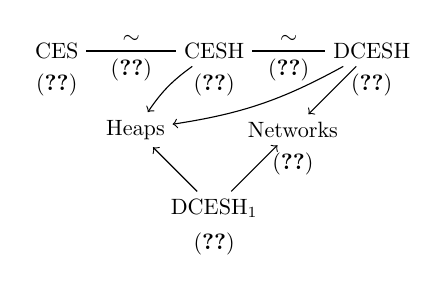
\begin{tikzpicture}[node distance=2.0cm, on grid,every node/.style={scale=0.8}]
  \node[label=below:(\ref{section:CES})]   (CES) {CES};
  \node[label=below:(\ref{section:CESH})]  (CESH) [right=of CES] {CESH};
  \node[label=below:(\ref{section:DCESH})] (DCESH) [right=of CESH] {\DCESHn};
\iffullversion
  \node[label=below:(\ref{section:Heaps})] (Heaps) [below left=1.0cm and 1.00cm of CESH] {Heaps};
\else
  \node (Heaps) [below left=1.0cm and 1.00cm of CESH] {Heaps};
\fi
  \node[label=below:(\ref{section:Networks})] (Networks) [below right=1.0cm and 1.00cm of CESH] {Networks};
  \node[label=below:(\ref{section:ADCESH})] (ADCESH) [below=of CESH] {\DCESHi};
\draw (CES) to node[above] {$\sim$}
                 node[below] {(\ref{section:CESH-bisim})}
                 (CESH);
  \draw (CESH) to node[above] {$\sim$}
                  node[below] {(\ref{section:DCESH-bisim})}
                  (DCESH);
\draw[->] (CESH) to[bend right=10] (Heaps);
  \draw[->] (DCESH) to[bend left=10] (Heaps);
  \draw[->] (DCESH) to (Networks);
  \draw[->] (ADCESH) to (Heaps);
  \draw[->] (ADCESH) to (Networks);
\end{tikzpicture}
\end{center}


\section{The CES machine} \label{section:CES}
Our goal is to make a compiler for a programming language with
locus specifiers that is based on conventional compilation techniques.
A very common technique is the usage of \emph{abstract machines} to describe
the evaluation at a level low enough to be used as a basis for compilation.
The starting point for our work is based on a variation of Landin's
well-studied SECD machine~\cite{Landin64} called Modern SECD~\cite{ModernSECD}.
Modern SECD itself can be traced back to the SECD machine of
Henderson~\cite{DBLP:books/daglib/0068837}, in that both use bytecode for the
control component of the 
\iffullversion
machine
(and so use explicit return instructions);
\else
machine;
\fi
and
to the CEK machine of Felleisen~\cite{Felleisen:1986:CEK}, in that they both
place the continuations that originally resided in the dump
\iffullversion
(the D component)
\fi
directly on the
\iffullversion
stack (the S component),
\else
stack,
\fi
simplifying the machine configurations.

We choose to call this variation the \emph{CES machine} because of its three
configuration constituents. This machine is important for us since it will be
used as the \emph{specification} for the elaborated machines that we later
construct. We will show that their termination and divergence behaviour is the
same as that of CES by constructing bisimulation relations.

A CES configuration ({\textsmaller[.5]{\ensuremath{\Conid{Config}}}}) is a tuple consisting of a fragment of code
({\textsmaller[.5]{\ensuremath{\Conid{Code}}}}), an environment ({\textsmaller[.5]{\ensuremath{\Conid{Env}}}}), and a stack ({\textsmaller[.5]{\ensuremath{\Conid{Stack}}}}).  Evaluation begins
with an empty stack and environment, and then follows a \emph{stack
discipline}. Sub-terms push their result on the stack so that their super-terms
can consume them. When (and if) the evaluation terminates, the program's result
is the sole stack element.
\paragraph*{Source language}
\begin{comment}
\begin{hscode}\SaveRestoreHook
\column{B}{@{}>{\hspre}l<{\hspost}@{}}\column{E}{@{}>{\hspre}l<{\hspost}@{}}\>[B]{}\Keyword{module}\;\Conid{Lambda}\;(\Conid{Node}\;\mathbin{:}\;\star)\;\Keyword{where}{}\<[E]\\
\>[B]{}\Keyword{open}\;\Keyword{import}\;\Conid{GeneralLemmas}{}\<[E]\\[\blanklineskip]\>[B]{}\Keyword{infixl}\;\Varid{1}\;{\dummy\MyConid{\$}\dummy}{}\<[E]\ColumnHook
\end{hscode}\resethooks
\end{comment}
We show how to compile untyped call-by-value PCF \cite{DBLP:journals/tcs/Plotkin77}.
The source language has constructors for lambda abstractions ({\textsmaller[.5]{\ensuremath{\MyConid{$\boldsymbol{\lambda}$}\;\Varid{t}}}}), applications ({\textsmaller[.5]{\ensuremath{\Varid{t}\;\MyConid{\$}\;\Varid{t'}}}}), and variables ({\textsmaller[.5]{\ensuremath{\MyConid{var}\;\Varid{n}}}}).  Our representation uses De Bruijn
indices \cite{DeBruijn}, so a variable is simply a natural number.
\ifnotfullversion
Additionally, we have natural number literals ({\textsmaller[.5]{\ensuremath{\MyConid{lit}\;\Varid{n}}}}), binary operations on
them ({\textsmaller[.5]{\ensuremath{\MyConid{op}\;\Varid{f}\;\Varid{t}\;\Varid{t'}}}}), and conditionals ({\textsmaller[.5]{\ensuremath{\MyConid{if0}\;\Varid{t}\;\MyConid{then}\;\Varid{t₀}\;\MyConid{else}\;\Varid{t₁}}}}).
\fi
\iffullversion
\savecolumns
\begin{hscode}\SaveRestoreHook
\column{B}{@{}>{\hspre}l<{\hspost}@{}}\column{3}{@{}>{\hspre}l<{\hspost}@{}}\column{9}{@{}>{\hspre}l<{\hspost}@{}}\column{E}{@{}>{\hspre}l<{\hspost}@{}}\>[B]{}\Keyword{data}\;\Conid{Term}\;\mathbin{:}\;\star\;\Keyword{where}{}\<[E]\\
\>[B]{}\hsindent{3}{}\<[3]\>[3]{}{\MyConid{$\boldsymbol{\lambda}$}\dummy}\;{}\<[9]\>[9]{}\mathbin{:}\;\Conid{Term}\;\Varid{→}\;\Conid{Term}{}\<[E]\\
\>[B]{}\hsindent{3}{}\<[3]\>[3]{}{\dummy\MyConid{\$}\dummy}\;{}\<[9]\>[9]{}\mathbin{:}\;(\Varid{t}\;\Varid{t'}\;\mathbin{:}\;\Conid{Term})\;\Varid{→}\;\Conid{Term}{}\<[E]\\
\>[B]{}\hsindent{3}{}\<[3]\>[3]{}\MyConid{var}\;{}\<[9]\>[9]{}\mathbin{:}\;\Conid{ℕ}\;\Varid{→}\;\Conid{Term}{}\<[E]\ColumnHook
\end{hscode}\resethooks
We also have natural number literals, binary operations on them, and
conditionals:
\restorecolumns
\begin{hscode}\SaveRestoreHook
\column{B}{@{}>{\hspre}l<{\hspost}@{}}\column{3}{@{}>{\hspre}l<{\hspost}@{}}\column{9}{@{}>{\hspre}l<{\hspost}@{}}\column{19}{@{}>{\hspre}l<{\hspost}@{}}\column{E}{@{}>{\hspre}l<{\hspost}@{}}\>[3]{}\MyConid{lit}\;{}\<[9]\>[9]{}\mathbin{:}\;\Conid{ℕ}\;\Varid{→}\;\Conid{Term}{}\<[E]\\
\>[3]{}\MyConid{op}\;{}\<[9]\>[9]{}\mathbin{:}\;(\Varid{f}\;\mathbin{:}\;\Conid{ℕ}\;\Varid{→}\;\Conid{ℕ}\;\Varid{→}\;\Conid{ℕ})\;(\Varid{t}\;\Varid{t'}\;\mathbin{:}\;\Conid{Term})\;\Varid{→}\;\Conid{Term}{}\<[E]\\
\>[3]{}{\MyConid{if0}\dummy\MyConid{then}\dummy\MyConid{else}\dummy}\;{}\<[19]\>[19]{}\mathbin{:}\;(\Varid{b}\;\Varid{t}\;\Varid{f}\;\mathbin{:}\;\Conid{Term})\;\Varid{→}\;\Conid{Term}{}\<[E]\ColumnHook
\end{hscode}\resethooks
\fi
\begin{comment}
\begin{hscode}\SaveRestoreHook
\column{B}{@{}>{\hspre}l<{\hspost}@{}}\column{3}{@{}>{\hspre}l<{\hspost}@{}}\column{9}{@{}>{\hspre}l<{\hspost}@{}}\column{E}{@{}>{\hspre}l<{\hspost}@{}}\>[3]{}{\dummy\MyConid{$\boldsymbol{@}$}\dummy}\;{}\<[9]\>[9]{}\mathbin{:}\;\Conid{Term}\;\Varid{→}\;\Conid{Node}\;\Varid{→}\;\Conid{Term}{}\<[E]\ColumnHook
\end{hscode}\resethooks
\end{comment}
\iffullversion
The language can be thought of as an intermediate representation for a
compiler which may expose a more sugary front-end language.
\fi
Because
\iffullversion
it
\else
the language
\fi
is untyped, we can express fixed-point combinators without adding additional
constructors.

\begin{comment}
\begin{hscode}\SaveRestoreHook
\column{B}{@{}>{\hspre}l<{\hspost}@{}}\column{E}{@{}>{\hspre}l<{\hspost}@{}}\>[B]{}\Keyword{module}\;\Conid{MachineCode}\;(\Conid{Node}\;\mathbin{:}\;\star)\;\Keyword{where}{}\<[E]\\[\blanklineskip]\>[B]{}\Keyword{open}\;\Keyword{import}\;\Conid{Data.List.Any}{}\<[E]\\
\>[B]{}\Keyword{open}\;\Conid{Membership-≡}{}\<[E]\\[\blanklineskip]\>[B]{}\Keyword{open}\;\Keyword{import}\;\Conid{GeneralLemmas}{}\<[E]\\
\>[B]{}\Keyword{open}\;\Keyword{import}\;\Conid{Lambda}\;\Conid{Node}{}\<[E]\ColumnHook
\end{hscode}\resethooks
\end{comment}

\iffullversion
We define the bytecode, {\textsmaller[.5]{\ensuremath{\Conid{Code}}}}, that the machine will operate on. A
fragment of {\textsmaller[.5]{\ensuremath{\Conid{Code}}}} is a list of instructions, {\textsmaller[.5]{\ensuremath{\Conid{Instr}}}}, terminated by
{\textsmaller[.5]{\ensuremath{\MyConid{END}}}}, {\textsmaller[.5]{\ensuremath{\MyConid{RET}}}}, or a conditional {\textsmaller[.5]{\ensuremath{\MyConid{COND}}}} which has code fragments for its
two branches:
\savecolumns
\begin{hscode}\SaveRestoreHook
\column{B}{@{}>{\hspre}l<{\hspost}@{}}\column{3}{@{}>{\hspre}l<{\hspost}@{}}\column{5}{@{}>{\hspre}l<{\hspost}@{}}\column{14}{@{}>{\hspre}l<{\hspost}@{}}\column{22}{@{}>{\hspre}l<{\hspost}@{}}\column{E}{@{}>{\hspre}l<{\hspost}@{}}\>[B]{}\Keyword{mutual}{}\<[E]\\
\>[B]{}\hsindent{3}{}\<[3]\>[3]{}\Keyword{data}\;\Conid{Instr}\;\mathbin{:}\;\star\;\Keyword{where}{}\<[E]\\
\>[3]{}\hsindent{2}{}\<[5]\>[5]{}\MyConid{VAR}\;{}\<[14]\>[14]{}\mathbin{:}\;\Conid{ℕ}\;{}\<[22]\>[22]{}\Varid{→}\;\Conid{Instr}{}\<[E]\\
\>[3]{}\hsindent{2}{}\<[5]\>[5]{}\MyConid{CLOS}\;{}\<[14]\>[14]{}\mathbin{:}\;\Conid{Code}\;{}\<[22]\>[22]{}\Varid{→}\;\Conid{Instr}{}\<[E]\\
\>[3]{}\hsindent{2}{}\<[5]\>[5]{}\MyConid{APPL}\;{}\<[14]\>[14]{}\mathbin{:}\;\Conid{Instr}{}\<[E]\\
\>[3]{}\hsindent{2}{}\<[5]\>[5]{}\MyConid{LIT}\;{}\<[14]\>[14]{}\mathbin{:}\;\Conid{ℕ}\;{}\<[22]\>[22]{}\Varid{→}\;\Conid{Instr}{}\<[E]\\
\>[3]{}\hsindent{2}{}\<[5]\>[5]{}\MyConid{OP}\;{}\<[14]\>[14]{}\mathbin{:}\;(\Conid{ℕ}\;\Varid{→}\;\Conid{ℕ}\;\Varid{→}\;\Conid{ℕ})\;\Varid{→}\;\Conid{Instr}{}\<[E]\ColumnHook
\end{hscode}\resethooks
\begin{comment}
\begin{hscode}\SaveRestoreHook
\column{B}{@{}>{\hspre}l<{\hspost}@{}}\column{5}{@{}>{\hspre}l<{\hspost}@{}}\column{14}{@{}>{\hspre}l<{\hspost}@{}}\column{E}{@{}>{\hspre}l<{\hspost}@{}}\>[5]{}\MyConid{REMOTE}\;{}\<[14]\>[14]{}\mathbin{:}\;\Conid{Code}\;\Varid{→}\;\Conid{Node}\;\Varid{→}\;\Conid{Instr}{}\<[E]\ColumnHook
\end{hscode}\resethooks
\end{comment}
\removecodespace
\restorecolumns
\begin{hscode}\SaveRestoreHook
\column{B}{@{}>{\hspre}l<{\hspost}@{}}\column{3}{@{}>{\hspre}l<{\hspost}@{}}\column{5}{@{}>{\hspre}l<{\hspost}@{}}\column{14}{@{}>{\hspre}l<{\hspost}@{}}\column{23}{@{}>{\hspre}l<{\hspost}@{}}\column{E}{@{}>{\hspre}l<{\hspost}@{}}\>[3]{}\Keyword{data}\;\Conid{Code}\;\mathbin{:}\;\star\;\Keyword{where}{}\<[E]\\
\>[3]{}\hsindent{2}{}\<[5]\>[5]{}{\dummy\MyConid{;}\dummy}\;{}\<[14]\>[14]{}\mathbin{:}\;\Conid{Instr}\;{}\<[23]\>[23]{}\Varid{→}\;\Conid{Code}\;\Varid{→}\;\Conid{Code}{}\<[E]\\
\>[3]{}\hsindent{2}{}\<[5]\>[5]{}\MyConid{COND}\;{}\<[14]\>[14]{}\mathbin{:}\;\Conid{Code}\;{}\<[23]\>[23]{}\Varid{→}\;\Conid{Code}\;\Varid{→}\;\Conid{Code}{}\<[E]\\
\>[3]{}\hsindent{2}{}\<[5]\>[5]{}\MyConid{END}\;{}\<[14]\>[14]{}\mathbin{:}\;\Conid{Code}{}\<[E]\\
\>[3]{}\hsindent{2}{}\<[5]\>[5]{}\MyConid{RET}\;{}\<[14]\>[14]{}\mathbin{:}\;\Conid{Code}{}\<[E]\ColumnHook
\end{hscode}\resethooks
\else
The machine operates on a bytecode and does not directly interpret the
source terms, so the terms need to be compiled before they can be
executed.
\fi
The main work of compilation is done by the function
{\textsmaller[.5]{\ensuremath{\Varid{compile'}}}}, which takes a term {\textsmaller[.5]{\ensuremath{\Varid{t}}}} to be compiled and a fragment of
code {\textsmaller[.5]{\ensuremath{\Varid{c}}}} that is placed after the instructions that the compilation
emits.
\ifnotfullversion
The bold upper-case names ({\textsmaller[.5]{\ensuremath{\MyConid{CLOS}}}}, {\textsmaller[.5]{\ensuremath{\MyConid{VAR}}}}, and so on) are the
bytecode instructions, which are sequenced using {\textsmaller[.5]{\ensuremath{{\dummy\MyConid{;}\dummy}}}}:
\fi
\begin{hscode}\SaveRestoreHook
\column{B}{@{}>{\hspre}l<{\hspost}@{}}\column{3}{@{}>{\hspre}l<{\hspost}@{}}\column{23}{@{}>{\hspre}l<{\hspost}@{}}\column{26}{@{}>{\hspre}l<{\hspost}@{}}\column{38}{@{}>{\hspre}l<{\hspost}@{}}\column{E}{@{}>{\hspre}l<{\hspost}@{}}\>[B]{}\Varid{compile'}\;\mathbin{:}\;\Conid{Term}\;\Varid{→}\;\Conid{Code}\;\Varid{→}\;\Conid{Code}{}\<[E]\\
\>[B]{}\Varid{compile'}\;(\MyConid{$\boldsymbol{\lambda}$}\;\Varid{t})\;{}\<[23]\>[23]{}\Varid{c}\;{}\<[26]\>[26]{}\mathrel{=}\;\MyConid{CLOS}\;(\Varid{compile'}\;\Varid{t}\;\MyConid{RET})\;\MyConid{;}\;\Varid{c}{}\<[E]\\
\>[B]{}\Varid{compile'}\;(\Varid{t}\;\MyConid{\$}\;\Varid{t'})\;{}\<[23]\>[23]{}\Varid{c}\;{}\<[26]\>[26]{}\mathrel{=}\;\Varid{compile'}\;{}\<[38]\>[38]{}\Varid{t}\;(\Varid{compile'}\;\Varid{t'}\;(\MyConid{APPL}\;\MyConid{;}\;\Varid{c})){}\<[E]\\
\>[B]{}\Varid{compile'}\;(\MyConid{var}\;\Varid{x})\;{}\<[23]\>[23]{}\Varid{c}\;{}\<[26]\>[26]{}\mathrel{=}\;\MyConid{VAR}\;\Varid{x}\;\MyConid{;}\;\Varid{c}{}\<[E]\\
\>[B]{}\Varid{compile'}\;(\MyConid{lit}\;\Varid{n})\;{}\<[23]\>[23]{}\Varid{c}\;{}\<[26]\>[26]{}\mathrel{=}\;\MyConid{LIT}\;\Varid{n}\;\MyConid{;}\;\Varid{c}{}\<[E]\\
\>[B]{}\Varid{compile'}\;(\MyConid{op}\;\Varid{f}\;\Varid{t}\;\Varid{t'})\;{}\<[23]\>[23]{}\Varid{c}\;{}\<[26]\>[26]{}\mathrel{=}\;\Varid{compile'}\;{}\<[38]\>[38]{}\Varid{t'}\;(\Varid{compile'}\;\Varid{t}\;(\MyConid{OP}\;\Varid{f}\;\MyConid{;}\;\Varid{c})){}\<[E]\\
\>[B]{}\Varid{compile'}\;(\MyConid{if0}\;\Varid{b}\;\MyConid{then}\;\Varid{t}\;\MyConid{else}\;\Varid{f})\;\Varid{c}\;\mathrel{=}\;{}\<[E]\\
\>[B]{}\hsindent{3}{}\<[3]\>[3]{}\Varid{compile'}\;\Varid{b}\;(\MyConid{COND}\;(\Varid{compile'}\;\Varid{t}\;\Varid{c})\;(\Varid{compile'}\;\Varid{f}\;\Varid{c})){}\<[E]\ColumnHook
\end{hscode}\resethooks
\begin{comment}
\begin{hscode}\SaveRestoreHook
\column{B}{@{}>{\hspre}l<{\hspost}@{}}\column{20}{@{}>{\hspre}l<{\hspost}@{}}\column{23}{@{}>{\hspre}l<{\hspost}@{}}\column{E}{@{}>{\hspre}l<{\hspost}@{}}\>[B]{}\Varid{compile'}\;(\Varid{t}\;\MyConid{$\boldsymbol{@}$}\;\Varid{i})\;{}\<[20]\>[20]{}\Varid{c}\;{}\<[23]\>[23]{}\mathrel{=}\;\MyConid{REMOTE}\;(\Varid{compile'}\;\Varid{t}\;\MyConid{RET})\;\Varid{i}\;\MyConid{;}\;\Varid{c}{}\<[E]\ColumnHook
\end{hscode}\resethooks
\end{comment}
It should be apparent that the instructions correspond closely
to the constructs of the source language but are sequentialised.
Compilation of a term is simply a call to {\textsmaller[.5]{\ensuremath{\Varid{compile'}}}}, terminated by
{\textsmaller[.5]{\ensuremath{\MyConid{END}}}}:
\iffullversion
\begin{hscode}\SaveRestoreHook
\column{B}{@{}>{\hspre}l<{\hspost}@{}}\column{E}{@{}>{\hspre}l<{\hspost}@{}}\>[B]{}\Varid{compile}\;\mathbin{:}\;\Conid{Term}\;\Varid{→}\;\Conid{Code}{}\<[E]\\
\>[B]{}\Varid{compile}\;\Varid{t}\;\mathrel{=}\;\Varid{compile'}\;\Varid{t}\;\MyConid{END}{}\<[E]\ColumnHook
\end{hscode}\resethooks
\else
{\textsmaller[.5]{\ensuremath{\Varid{compile}\;\Varid{t}\;\mathrel{=}\;\Varid{compile'}\;\Varid{t}\;\MyConid{END}}}}.
\fi
\begin{example}[{\textsmaller[.5]{\ensuremath{\Varid{codeExample}}}}]
The term {\textsmaller[.5]{\ensuremath{(\Varid{λx.}\;\Varid{x})\;(\Varid{λx}\;\Varid{y.}\;\Varid{x})}}} is compiled as follows:
\begin{comment}
\begin{hscode}\SaveRestoreHook
\column{B}{@{}>{\hspre}l<{\hspost}@{}}\column{E}{@{}>{\hspre}l<{\hspost}@{}}\>[B]{}\Varid{codeExample}\;\mathrel{=}\;\Varid{compile}\;((\MyConid{$\boldsymbol{\lambda}$}\;\MyConid{var}\;\Varid{0})\;\MyConid{\$}\;(\MyConid{$\boldsymbol{\lambda}$}\;(\MyConid{$\boldsymbol{\lambda}$}\;\MyConid{var}\;\Varid{1}))){}\<[E]\ColumnHook
\end{hscode}\resethooks
\end{comment}
\begin{hscode}\SaveRestoreHook
\column{B}{@{}>{\hspre}l<{\hspost}@{}}\column{3}{@{}>{\hspre}l<{\hspost}@{}}\column{E}{@{}>{\hspre}l<{\hspost}@{}}\>[B]{}\Varid{compile}\;((\MyConid{$\boldsymbol{\lambda}$}\;\MyConid{var}\;\Varid{0})\;\MyConid{\$}\;(\MyConid{$\boldsymbol{\lambda}$}\;(\MyConid{$\boldsymbol{\lambda}$}\;\MyConid{var}\;\Varid{1})))\;\mathrel{=}\;{}\<[E]\\
\>[B]{}\hsindent{3}{}\<[3]\>[3]{}\MyConid{CLOS}\;(\MyConid{VAR}\;\Varid{0}\;\MyConid{;}\;\MyConid{RET})\;\MyConid{;}\;{}\<[E]\\
\>[B]{}\hsindent{3}{}\<[3]\>[3]{}\MyConid{CLOS}\;(\MyConid{CLOS}\;(\MyConid{VAR}\;\Varid{1}\;\MyConid{;}\;\MyConid{RET})\;\MyConid{;}\;\MyConid{RET})\;\MyConid{;}\;\MyConid{APPL}\;\MyConid{;}\;\MyConid{END}{}\<[E]\ColumnHook
\end{hscode}\resethooks
Compilation first emits two {\textsmaller[.5]{\ensuremath{\MyConid{CLOS}}}} instructions containing the code
of the function and its argument. The {\textsmaller[.5]{\ensuremath{\MyConid{APPL}}}} instruction is then used to
perform the actual application.
\end{example}
\begin{comment}
\begin{hscode}\SaveRestoreHook
\column{B}{@{}>{\hspre}l<{\hspost}@{}}\column{E}{@{}>{\hspre}l<{\hspost}@{}}\>[B]{}\Keyword{module}\;\Conid{CES}\;(\Conid{Node}\;\mathbin{:}\;\star)\;\Keyword{where}{}\<[E]\\[\blanklineskip]\>[B]{}\Keyword{open}\;\Keyword{import}\;\Conid{GeneralLemmas}{}\<[E]\\[\blanklineskip]\>[B]{}\Keyword{open}\;\Keyword{import}\;\Conid{MachineCode}\;\Conid{Node}{}\<[E]\\
\>[B]{}\Keyword{open}\;\Keyword{import}\;\Conid{Relation}{}\<[E]\ColumnHook
\end{hscode}\resethooks
\end{comment}

\ifnotfullversion
Environments ({\textsmaller[.5]{\ensuremath{\Conid{Env}}}}) are lists of values ({\textsmaller[.5]{\ensuremath{\Conid{List}\;\Conid{Value}}}}).  A value is
either a natural number ({\textsmaller[.5]{\ensuremath{\MyConid{nat}\;\Varid{n}}}}) or a closure ({\textsmaller[.5]{\ensuremath{\MyConid{clos}\;\Varid{cl}}}}).  A closure ({\textsmaller[.5]{\ensuremath{\Conid{Closure}}}})
is a fragment of code paired with an environment ({\textsmaller[.5]{\ensuremath{\Conid{Code}\;\Varid{×}\;\Conid{Env}}}}).
\else
We mutually define values, closures and environments. A closure is a
code fragment paired with an environment. A value is either a natural
number literal or a closure.  Since we are working in a call-by-value
setting an environment is a list of values.
\begin{hscode}\SaveRestoreHook
\column{B}{@{}>{\hspre}l<{\hspost}@{}}\column{3}{@{}>{\hspre}l<{\hspost}@{}}\column{5}{@{}>{\hspre}l<{\hspost}@{}}\column{11}{@{}>{\hspre}l<{\hspost}@{}}\column{22}{@{}>{\hspre}l<{\hspost}@{}}\column{E}{@{}>{\hspre}l<{\hspost}@{}}\>[B]{}\Keyword{mutual}{}\<[E]\\
\>[B]{}\hsindent{3}{}\<[3]\>[3]{}\Conid{Closure}\;\mathrel{=}\;\Conid{Code}\;\Varid{×}\;\Conid{Env}{}\<[E]\\
\>[B]{}\hsindent{3}{}\<[3]\>[3]{}\Keyword{data}\;\Conid{Value}\;\mathbin{:}\;\star\;\Keyword{where}{}\<[E]\\
\>[3]{}\hsindent{2}{}\<[5]\>[5]{}\MyConid{nat}\;{}\<[11]\>[11]{}\mathbin{:}\;\Conid{ℕ}\;{}\<[22]\>[22]{}\Varid{→}\;\Conid{Value}{}\<[E]\\
\>[3]{}\hsindent{2}{}\<[5]\>[5]{}\MyConid{clos}\;{}\<[11]\>[11]{}\mathbin{:}\;\Conid{Closure}\;{}\<[22]\>[22]{}\Varid{→}\;\Conid{Value}{}\<[E]\\
\>[B]{}\hsindent{3}{}\<[3]\>[3]{}\Conid{Env}\;\mathrel{=}\;\Conid{List}\;\Conid{Value}{}\<[E]\ColumnHook
\end{hscode}\resethooks
\fi
\ifnotfullversion
Stacks ({\textsmaller[.5]{\ensuremath{\Conid{Stack}}}}) are lists of stack elements ({\textsmaller[.5]{\ensuremath{\Conid{List}\;\Conid{StackElem}}}}), where
stack elements are either values ({\textsmaller[.5]{\ensuremath{\MyConid{val}\;\Varid{v}}}}) or continuations ({\textsmaller[.5]{\ensuremath{\MyConid{cont}\;\Varid{cl}}}}), represented by closures.
\else
A stack is a list of stack elements, defined to be either values
or continuations (represented by closures):
\begin{hscode}\SaveRestoreHook
\column{B}{@{}>{\hspre}l<{\hspost}@{}}\column{3}{@{}>{\hspre}l<{\hspost}@{}}\column{9}{@{}>{\hspre}l<{\hspost}@{}}\column{20}{@{}>{\hspre}l<{\hspost}@{}}\column{E}{@{}>{\hspre}l<{\hspost}@{}}\>[B]{}\Keyword{data}\;\Conid{StackElem}\;\mathbin{:}\;\star\;\Keyword{where}{}\<[E]\\
\>[B]{}\hsindent{3}{}\<[3]\>[3]{}\MyConid{val}\;{}\<[9]\>[9]{}\mathbin{:}\;\Conid{Value}\;{}\<[20]\>[20]{}\Varid{→}\;\Conid{StackElem}{}\<[E]\\
\>[B]{}\hsindent{3}{}\<[3]\>[3]{}\MyConid{cont}\;{}\<[9]\>[9]{}\mathbin{:}\;\Conid{Closure}\;{}\<[20]\>[20]{}\Varid{→}\;\Conid{StackElem}{}\<[E]\\
\>[B]{}\Conid{Stack}\;\mathrel{=}\;\Conid{List}\;\Conid{StackElem}{}\<[E]\ColumnHook
\end{hscode}\resethooks
A configuration is, as stated, a tuple consisting of a code fragment, an
environment and a stack:
\begin{hscode}\SaveRestoreHook
\column{B}{@{}>{\hspre}l<{\hspost}@{}}\column{E}{@{}>{\hspre}l<{\hspost}@{}}\>[B]{}\Conid{Config}\;\mathrel{=}\;\Conid{Code}\;\Varid{×}\;\Conid{Env}\;\Varid{×}\;\Conid{Stack}{}\<[E]\ColumnHook
\end{hscode}\resethooks
\fi

\iffullversion
\begin{sidewaysfigure}
\else
\begin{figure*}[!t]
\fi
\centering
\begin{varwidth}[t]{\textwidth}
\rightaligncolumn{36}
\rightaligncolumn{54}
\indentcolumn{3}
\iffullversion
\begin{hscode}\SaveRestoreHook
\column{B}{@{}>{\hspre}l<{\hspost}@{}}\column{E}{@{}>{\hspre}l<{\hspost}@{}}\>[B]{}\Keyword{data}\;{\dummy\xrightarrow[\Varid{CES}]{}\dummy}\;\mathbin{:}\;\Conid{Rel}\;\Conid{Config}\;\Conid{Config}\;\Keyword{where}{}\<[E]\ColumnHook
\end{hscode}\resethooks
\removecodespace
\indentcolumn{3}
\fi
\begin{hscode}\SaveRestoreHook
\column{B}{@{}>{\hspre}l<{\hspost}@{}}\column{3}{@{}>{\hspre}l<{\hspost}@{}}\column{13}{@{}>{\hspre}l<{\hspost}@{}}\column{36}{@{}>{\hspre}l<{\hspost}@{}}\column{54}{@{}>{\hspre}l<{\hspost}@{}}\column{92}{@{}>{\hspre}l<{\hspost}@{}}\column{103}{@{}>{\hspre}l<{\hspost}@{}}\column{105}{@{}>{\hspre}l<{\hspost}@{}}\column{E}{@{}>{\hspre}l<{\hspost}@{}}\>[3]{}\MyConid{VAR}\;{}\<[13]\>[13]{}\mathbin{:}\;\Varid{∀}\;\{\mskip1.5mu \Varid{n}\;\Varid{c}\;\Varid{e}\;\Varid{s}\;\Varid{v}\mskip1.5mu\}\;\Varid{→}\;\Varid{lookup}\;\Varid{n}\;\Varid{e}\;\Varid{≡}\;\MyConid{just}\;\Varid{v}\;\Varid{→}\;{}\<[54]\>[54]{}(\MyConid{VAR}\;\Varid{n}\;\MyConid{;}\;\Varid{c},\Varid{e},\Varid{s})\;{}\<[92]\>[92]{}\xrightarrow[\Varid{CES}]{}\;(\Varid{c},{}\<[105]\>[105]{}\Varid{e},\MyConid{val}\;\Varid{v}\;\Varid{∷}\;\Varid{s}){}\<[E]\\
\>[3]{}\MyConid{CLOS}\;{}\<[13]\>[13]{}\mathbin{:}\;\Varid{∀}\;\{\mskip1.5mu \Varid{c'}\;\Varid{c}\;\Varid{e}\;\Varid{s}\mskip1.5mu\}\;\Varid{→}\;{}\<[36]\>[36]{}(\MyConid{CLOS}\;\Varid{c'}\;\MyConid{;}\;\Varid{c},\Varid{e},\Varid{s})\;{}\<[92]\>[92]{}\xrightarrow[\Varid{CES}]{}\;(\Varid{c},{}\<[103]\>[103]{}\Varid{e},\MyConid{val}\;(\MyConid{clos}\;(\Varid{c'},\Varid{e}))\;\Varid{∷}\;\Varid{s}){}\<[E]\\
\>[3]{}\MyConid{APPL}\;{}\<[13]\>[13]{}\mathbin{:}\;\Varid{∀}\;\{\mskip1.5mu \Varid{c}\;\Varid{e}\;\Varid{v}\;\Varid{c'}\;\Varid{e'}\;\Varid{s}\mskip1.5mu\}\;\Varid{→}\;{}\<[36]\>[36]{}(\MyConid{APPL}\;\MyConid{;}\;\Varid{c},\Varid{e},\MyConid{val}\;\Varid{v}\;\Varid{∷}\;\MyConid{val}\;(\MyConid{clos}\;(\Varid{c'},\Varid{e'}))\;\Varid{∷}\;\Varid{s})\;{}\<[92]\>[92]{}\xrightarrow[\Varid{CES}]{}\;(\Varid{c'},\Varid{v}\;\Varid{∷}\;\Varid{e'},\MyConid{cont}\;(\Varid{c},\Varid{e})\;\Varid{∷}\;\Varid{s}){}\<[E]\\
\>[3]{}\MyConid{RET}\;{}\<[13]\>[13]{}\mathbin{:}\;\Varid{∀}\;\{\mskip1.5mu \Varid{e}\;\Varid{v}\;\Varid{c}\;\Varid{e'}\;\Varid{s}\mskip1.5mu\}\;\Varid{→}\;{}\<[36]\>[36]{}(\MyConid{RET},\Varid{e},\MyConid{val}\;\Varid{v}\;\Varid{∷}\;\MyConid{cont}\;(\Varid{c},\Varid{e'})\;\Varid{∷}\;\Varid{s})\;{}\<[92]\>[92]{}\xrightarrow[\Varid{CES}]{}\;(\Varid{c},\Varid{e'},\MyConid{val}\;\Varid{v}\;\Varid{∷}\;\Varid{s}){}\<[E]\\
\>[3]{}\MyConid{LIT}\;{}\<[13]\>[13]{}\mathbin{:}\;\Varid{∀}\;\{\mskip1.5mu \Varid{n}\;\Varid{c}\;\Varid{e}\;\Varid{s}\mskip1.5mu\}\;\Varid{→}\;{}\<[36]\>[36]{}(\MyConid{LIT}\;\Varid{n}\;\MyConid{;}\;\Varid{c},\Varid{e},\Varid{s})\;{}\<[92]\>[92]{}\xrightarrow[\Varid{CES}]{}\;(\Varid{c},\Varid{e},\MyConid{val}\;(\MyConid{nat}\;\Varid{n})\;\Varid{∷}\;\Varid{s}){}\<[E]\\
\>[3]{}\MyConid{OP}\;{}\<[13]\>[13]{}\mathbin{:}\;\Varid{∀}\;\{\mskip1.5mu \Varid{f}\;\Varid{c}\;\Varid{e}\;\Varid{n₁}\;\Varid{n₂}\;\Varid{s}\mskip1.5mu\}\;\Varid{→}\;{}\<[36]\>[36]{}(\MyConid{OP}\;\Varid{f}\;\MyConid{;}\;\Varid{c},\Varid{e},\MyConid{val}\;(\MyConid{nat}\;\Varid{n₁})\;\Varid{∷}\;\MyConid{val}\;(\MyConid{nat}\;\Varid{n₂})\;\Varid{∷}\;\Varid{s})\;{}\<[92]\>[92]{}\xrightarrow[\Varid{CES}]{}\;(\Varid{c},\Varid{e},\MyConid{val}\;(\MyConid{nat}\;(\Varid{f}\;\Varid{n₁}\;\Varid{n₂}))\;\Varid{∷}\;\Varid{s}){}\<[E]\\
\>[3]{}\MyConid{COND-0}\;{}\<[13]\>[13]{}\mathbin{:}\;\Varid{∀}\;\{\mskip1.5mu \Varid{c}\;\Varid{c'}\;\Varid{e}\;\Varid{s}\mskip1.5mu\}\;\Varid{→}\;{}\<[36]\>[36]{}(\MyConid{COND}\;\Varid{c}\;\Varid{c'},\Varid{e},\MyConid{val}\;(\MyConid{nat}\;\Varid{0})\;\Varid{∷}\;\Varid{s})\;{}\<[92]\>[92]{}\xrightarrow[\Varid{CES}]{}\;(\Varid{c},\Varid{e},\Varid{s}){}\<[E]\\
\>[3]{}\MyConid{COND-1+n}\;{}\<[13]\>[13]{}\mathbin{:}\;\Varid{∀}\;\{\mskip1.5mu \Varid{c}\;\Varid{c'}\;\Varid{e}\;\Varid{n}\;\Varid{s}\mskip1.5mu\}\;\Varid{→}\;{}\<[36]\>[36]{}(\MyConid{COND}\;\Varid{c}\;\Varid{c'},\Varid{e},\MyConid{val}\;(\MyConid{nat}\;(1+\;\Varid{n}))\;\Varid{∷}\;\Varid{s})\;{}\<[92]\>[92]{}\xrightarrow[\Varid{CES}]{}\;(\Varid{c'},\Varid{e},\Varid{s}){}\<[E]\ColumnHook
\end{hscode}\resethooks
\begin{comment}
\begin{hscode}\SaveRestoreHook
\column{B}{@{}>{\hspre}l<{\hspost}@{}}\column{3}{@{}>{\hspre}l<{\hspost}@{}}\column{12}{@{}>{\hspre}l<{\hspost}@{}}\column{E}{@{}>{\hspre}l<{\hspost}@{}}\>[3]{}\MyConid{REMOTE}\;\mathbin{:}\;\Varid{∀}\;\{\mskip1.5mu \Varid{c'}\;\Varid{i}\;\Varid{c}\;\Varid{e}\;\Varid{s}\mskip1.5mu\}\;\Varid{→}\;{}\<[E]\\
\>[3]{}\hsindent{9}{}\<[12]\>[12]{}(\MyConid{REMOTE}\;\Varid{c'}\;\Varid{i}\;\MyConid{;}\;\Varid{c},\Varid{e},\Varid{s})\;\xrightarrow[\Varid{CES}]{}\;(\Varid{c'},[\mskip1.5mu \mskip1.5mu],\MyConid{cont}\;(\Varid{c},\Varid{e})\;\Varid{∷}\;\Varid{s}){}\<[E]\ColumnHook
\end{hscode}\resethooks
\end{comment}
\end{varwidth}
\caption{The definition of the transition relation of the CES machine.}
\label{figure:CES-step}
\iffullversion
\end{sidewaysfigure}
\else
\end{figure*}
\fi


Fig.~\ref{figure:CES-step} shows the definition of the transition
relation for configurations of the CES machine. The Agda syntax may
require some further explanation: The instructions' constructor names
are overloaded to also act as constructors for the relation; their
usage will be disambiguated by context. We use \emph{implicit
arguments}, written in curly braces, for arguments that can automatically
be inferred and do not need to be spelled out explicitly. The type of
propositional equality is written {\textsmaller[.5]{\ensuremath{\Varid{\char95 ≡\char95 }}}}.

The stack discipline becomes apparent in the definition of the
transition relation.  When e.g. {\textsmaller[.5]{\ensuremath{\MyConid{VAR}}}} is executed, the CES machine looks up
the value of the variable in the environment and pushes it on the
stack.  A somewhat subtle part of the relation is the interplay
between the {\textsmaller[.5]{\ensuremath{\MyConid{APPL}}}} instruction and the {\textsmaller[.5]{\ensuremath{\MyConid{RET}}}} instruction. When
performing an application, two values are required on the stack, one of
which has to be a closure.  The machine enters the closure, adding the
value to the environment, and pushes a return continuation on the
stack.  Looking at the {\textsmaller[.5]{\ensuremath{\Varid{compile}}}} function, we see that the code inside
a closure will be terminated by a {\textsmaller[.5]{\ensuremath{\MyConid{RET}}}} instruction, so once the
machine has finished executing the closure (and thus produced a value
on the stack), that value is returned to the continuation.

\begin{example} \label{example:CES}
We trace the execution of {\textsmaller[.5]{\ensuremath{\Varid{codeExample}}}} defined above, which exemplifies
how returning from an application works. Here we write {\textsmaller[.5]{\ensuremath{\Varid{a}\;\xrightarrow[\Varid{CES}]{}\Varid{⟨}\;\Varid{x}\;\Varid{⟩}\;\Varid{b}}}}
meaning that the machine uses rule {\textsmaller[.5]{\ensuremath{\Varid{x}}}} to transition from {\textsmaller[.5]{\ensuremath{\Varid{a}}}} to {\textsmaller[.5]{\ensuremath{\Varid{b}}}}.
\begin{hscode}\SaveRestoreHook
\column{B}{@{}>{\hspre}l<{\hspost}@{}}\column{6}{@{}>{\hspre}l<{\hspost}@{}}\column{11}{@{}>{\hspre}l<{\hspost}@{}}\column{16}{@{}>{\hspre}l<{\hspost}@{}}\column{36}{@{}>{\hspre}l<{\hspost}@{}}\column{41}{@{}>{\hspre}l<{\hspost}@{}}\column{E}{@{}>{\hspre}l<{\hspost}@{}}\>[B]{}\Keyword{let}\;{}\<[6]\>[6]{}\Varid{c₁}\;{}\<[11]\>[11]{}\mathrel{=}\;\MyConid{VAR}\;\Varid{0}\;\MyConid{;}\;\MyConid{RET}{}\<[E]\\
\>[6]{}\Varid{c₂}\;{}\<[11]\>[11]{}\mathrel{=}\;\MyConid{CLOS}\;(\MyConid{VAR}\;\Varid{1}\;\MyConid{;}\;\MyConid{RET})\;\MyConid{;}\;\MyConid{RET}{}\<[E]\\
\>[6]{}\Varid{cl₁}\;{}\<[11]\>[11]{}\mathrel{=}\;\MyConid{val}\;(\MyConid{clos}\;(\Varid{c₁},[\mskip1.5mu \mskip1.5mu]));{}\<[36]\>[36]{}\Varid{cl₂}\;{}\<[41]\>[41]{}\mathrel{=}\;\MyConid{val}\;(\MyConid{clos}\;(\Varid{c₂},[\mskip1.5mu \mskip1.5mu])){}\<[E]\\
\>[B]{}\Keyword{in}\;(\MyConid{CLOS}\;\Varid{c₁}\;\MyConid{;}\;\MyConid{CLOS}\;\Varid{c₂}\;\MyConid{;}\;\MyConid{APPL}\;\MyConid{;}\;\MyConid{END},[\mskip1.5mu \mskip1.5mu],[\mskip1.5mu \mskip1.5mu]){}\<[E]\\
\>[B]{}\xrightarrow[\Varid{CES}]{}\Varid{⟨}\;\MyConid{CLOS}\;\Varid{⟩}\;{}\<[16]\>[16]{}(\MyConid{CLOS}\;\Varid{c₂}\;\MyConid{;}\;\MyConid{APPL}\;\MyConid{;}\;\MyConid{END},[\mskip1.5mu \mskip1.5mu],[\mskip1.5mu \Varid{cl₁}\mskip1.5mu]){}\<[E]\\
\>[B]{}\xrightarrow[\Varid{CES}]{}\Varid{⟨}\;\MyConid{CLOS}\;\Varid{⟩}\;{}\<[16]\>[16]{}(\MyConid{APPL}\;\MyConid{;}\;\MyConid{END},[\mskip1.5mu \mskip1.5mu],[\mskip1.5mu \Varid{cl₂},\Varid{cl₁}\mskip1.5mu]){}\<[E]\\
\>[B]{}\xrightarrow[\Varid{CES}]{}\Varid{⟨}\;\MyConid{APPL}\;\Varid{⟩}\;{}\<[16]\>[16]{}(\MyConid{VAR}\;\Varid{0}\;\MyConid{;}\;\MyConid{RET},[\mskip1.5mu \Varid{cl₂}\mskip1.5mu],[\mskip1.5mu \MyConid{cont}\;(\MyConid{END},[\mskip1.5mu \mskip1.5mu])\mskip1.5mu]){}\<[E]\\
\>[B]{}\xrightarrow[\Varid{CES}]{}\Varid{⟨}\;\MyConid{VAR}\;\Varid{refl}\;\Varid{⟩}\;{}\<[16]\>[16]{}(\MyConid{RET},[\mskip1.5mu \Varid{cl₂}\mskip1.5mu],[\mskip1.5mu \Varid{cl₂},\MyConid{cont}\;(\MyConid{END},[\mskip1.5mu \mskip1.5mu])\mskip1.5mu]){}\<[E]\\
\>[B]{}\xrightarrow[\Varid{CES}]{}\Varid{⟨}\;\MyConid{RET}\;\Varid{⟩}\;{}\<[16]\>[16]{}(\MyConid{END},[\mskip1.5mu \mskip1.5mu],[\mskip1.5mu \Varid{cl₂}\mskip1.5mu]){}\<[E]\ColumnHook
\end{hscode}\resethooks
The final result is therefore the second closure, {\textsmaller[.5]{\ensuremath{\Varid{cl₂}}}}.
\end{example}
\begin{comment}
\begin{hscode}\SaveRestoreHook
\column{B}{@{}>{\hspre}l<{\hspost}@{}}\column{E}{@{}>{\hspre}l<{\hspost}@{}}\>[B]{}\Keyword{module}\;\Conid{CES.Properties}\;(\Conid{Node}\;\mathbin{:}\;\star)\;\Keyword{where}{}\<[E]\\
\>[B]{}\Keyword{open}\;\Keyword{import}\;\Conid{GeneralLemmas}{}\<[E]\\[\blanklineskip]\>[B]{}\Keyword{open}\;\Keyword{import}\;\Conid{MachineCode}\;\Conid{Node}{}\<[E]\\
\>[B]{}\Keyword{open}\;\Keyword{import}\;\Conid{CES}\;\Conid{Node}{}\<[E]\\
\>[B]{}\Keyword{open}\;\Keyword{import}\;\Conid{Relation}{}\<[E]\ColumnHook
\end{hscode}\resethooks
\end{comment}

\begin{lemma}[{\textsmaller[.5]{\ensuremath{\Varid{determinism}_{\Varid{CES}}}}}] {\textsmaller[.5]{\ensuremath{\xrightarrow[\Varid{CES}]{}}}} is deterministic.
\iffullversion
In the formalisation this means that we can construct the following term:
\begin{hscode}\SaveRestoreHook
\column{B}{@{}>{\hspre}l<{\hspost}@{}}\column{E}{@{}>{\hspre}l<{\hspost}@{}}\>[B]{}\Varid{determinism}_{\Varid{CES}}\;\mathbin{:}\;{\dummy\xrightarrow[\Varid{CES}]{}\dummy}\;\Varid{is-deterministic}{}\<[E]\ColumnHook
\end{hscode}\resethooks
where the type {\textsmaller[.5]{\ensuremath{\Varid{\char95 is-deterministic}}}} is defined as follows:
\begin{hscode}\SaveRestoreHook
\column{B}{@{}>{\hspre}l<{\hspost}@{}}\column{3}{@{}>{\hspre}l<{\hspost}@{}}\column{E}{@{}>{\hspre}l<{\hspost}@{}}\>[B]{}\Varid{\char95 is-deterministic}\;\mathbin{:}\;\{\mskip1.5mu \Conid{A}\;\Conid{B}\;\mathbin{:}\;\star\mskip1.5mu\}\;\Varid{→}\;\Conid{Rel}\;\Conid{A}\;\Conid{B}\;\Varid{→}\;\star{}\<[E]\\
\>[B]{}\Conid{R}\;\Varid{is-deterministic}\;\mathrel{=}\;{}\<[E]\\
\>[B]{}\hsindent{3}{}\<[3]\>[3]{}\Varid{∀}\;\{\mskip1.5mu \Varid{a}\;\Varid{b}\;\Varid{b'}\mskip1.5mu\}\;\Varid{→}\;\Conid{R}\;\Varid{a}\;\Varid{b}\;\Varid{→}\;\Conid{R}\;\Varid{a}\;\Varid{b'}\;\Varid{→}\;\Varid{b}\;\Varid{≡}\;\Varid{b'}{}\<[E]\ColumnHook
\end{hscode}\resethooks
\fi
\end{lemma}
This is a key property that is useful when constructing a compiler
implementation of the CES machine. Note that we write the name
of the definition containing this proof in parentheses.

\begin{comment}
\begin{hscode}\SaveRestoreHook
\column{B}{@{}>{\hspre}l<{\hspost}@{}}\column{3}{@{}>{\hspre}l<{\hspost}@{}}\column{9}{@{}>{\hspre}l<{\hspost}@{}}\column{26}{@{}>{\hspre}l<{\hspost}@{}}\column{36}{@{}>{\hspre}l<{\hspost}@{}}\column{E}{@{}>{\hspre}l<{\hspost}@{}}\>[B]{}\Varid{determinism}_{\Varid{CES}}\;(\MyConid{VAR}\;\Varid{x})\;(\MyConid{VAR}\;\Varid{y})\;{}\<[E]\\
\>[B]{}\hsindent{3}{}\<[3]\>[3]{}\mathrel{=}\;\Varid{cong}\;(\Varid{λ}\;\Varid{v}\;\Varid{→}\;\anonymous ,\anonymous ,\MyConid{val}\;\Varid{v}\;\Varid{∷}\;\anonymous )\;(\Varid{just-inj}\;(\Varid{trans}\;(\Varid{sym}\;\Varid{x})\;\Varid{y})){}\<[E]\\
\>[B]{}\Varid{determinism}_{\Varid{CES}}\;\MyConid{CLOS}\;{}\<[26]\>[26]{}\MyConid{CLOS}\;{}\<[36]\>[36]{}\mathrel{=}\;\Varid{refl}{}\<[E]\\
\>[B]{}\Varid{determinism}_{\Varid{CES}}\;\MyConid{APPL}\;{}\<[26]\>[26]{}\MyConid{APPL}\;{}\<[36]\>[36]{}\mathrel{=}\;\Varid{refl}{}\<[E]\\
\>[B]{}\Varid{determinism}_{\Varid{CES}}\;\MyConid{RET}\;{}\<[26]\>[26]{}\MyConid{RET}\;{}\<[36]\>[36]{}\mathrel{=}\;\Varid{refl}{}\<[E]\\
\>[B]{}\Varid{determinism}_{\Varid{CES}}\;\MyConid{REMOTE}\;{}\<[26]\>[26]{}\MyConid{REMOTE}\;{}\<[36]\>[36]{}\mathrel{=}\;\Varid{refl}{}\<[E]\\
\>[B]{}\Varid{determinism}_{\Varid{CES}}\;\MyConid{LIT}\;{}\<[26]\>[26]{}\MyConid{LIT}\;{}\<[36]\>[36]{}\mathrel{=}\;\Varid{refl}{}\<[E]\\
\>[B]{}\Varid{determinism}_{\Varid{CES}}\;\MyConid{OP}\;{}\<[26]\>[26]{}\MyConid{OP}\;{}\<[36]\>[36]{}\mathrel{=}\;\Varid{refl}{}\<[E]\\
\>[B]{}\Varid{determinism}_{\Varid{CES}}\;\MyConid{COND-0}\;{}\<[26]\>[26]{}\MyConid{COND-0}\;{}\<[36]\>[36]{}\mathrel{=}\;\Varid{refl}{}\<[E]\\
\>[B]{}\Varid{determinism}_{\Varid{CES}}\;\MyConid{COND-1+n}\;\MyConid{COND-1+n}\;{}\<[36]\>[36]{}\mathrel{=}\;\Varid{refl}{}\<[E]\\[\blanklineskip]\>[B]{}\Varid{⟶CES-is-decidable}\;\mathbin{:}\;{\dummy\xrightarrow[\Varid{CES}]{}\dummy}\;\Varid{is-decidable}{}\<[E]\\
\>[B]{}\Varid{⟶CES-is-decidable}\;(\MyConid{VAR}\;\Varid{n}\;\MyConid{;}\;\Varid{c},\Varid{e},\Varid{s})\;\Keyword{with}\;\Varid{lookup}\;\Varid{n}\;\Varid{e}\;\mid \;\Varid{inspect}\;(\Varid{lookup}\;\Varid{n})\;\Varid{e}{}\<[E]\\
\>[B]{}\Varid{⟶CES-is-decidable}\;(\MyConid{VAR}\;\Varid{n}\;\MyConid{;}\;\Varid{c},\Varid{e},\Varid{s})\;\mid \;\MyConid{just}\;\Varid{v}\;\mid \;[\mskip1.5mu \Varid{lu}\mskip1.5mu]\;\mathrel{=}\;\Varid{yes}\;((\Varid{c},\Varid{e},\MyConid{val}\;\Varid{v}\;\Varid{∷}\;\Varid{s}),\MyConid{VAR}\;\Varid{lu}){}\<[E]\\
\>[B]{}\Varid{⟶CES-is-decidable}\;(\MyConid{VAR}\;\Varid{n}\;\MyConid{;}\;\Varid{c},\Varid{e},\Varid{s})\;\mid \;\MyConid{nothing}\;\mid \;[\mskip1.5mu \Varid{lu}\mskip1.5mu]\;\mathrel{=}\;\Varid{no}\;(\Varid{lemma}\;\Varid{lu}){}\<[E]\\
\>[B]{}\hsindent{3}{}\<[3]\>[3]{}\Keyword{where}\;\Varid{lemma}\;\mathbin{:}\;\Varid{∀}\;\{\mskip1.5mu \Varid{n}\;\Varid{c}\;\Varid{e}\;\Varid{s}\mskip1.5mu\}\;\Varid{→}\;\Varid{lookup}\;\Varid{n}\;\Varid{e}\;\Varid{≡}\;\MyConid{nothing}\;\Varid{→}\;\Varid{∃}\;(\Varid{λ}\;\Varid{cfg}\;\Varid{→}\;(\MyConid{VAR}\;\Varid{n}\;\MyConid{;}\;\Varid{c},\Varid{e},\Varid{s})\;\xrightarrow[\Varid{CES}]{}\;\Varid{cfg})\;\Varid{→}\;\Varid{⊥}{}\<[E]\\
\>[3]{}\hsindent{6}{}\<[9]\>[9]{}\Varid{lemma}\;\Varid{lu}\;((\Varid{c},\Varid{e},\MyConid{val}\;\Varid{.v}\;\Varid{∷}\;\Varid{s}),\MyConid{VAR}\;\{\mskip1.5mu \Varid{v}\;\mathrel{=}\;\Varid{v}\mskip1.5mu\}\;\Varid{lu'})\;\mathrel{=}\;\Varid{nothing≠just}\;(\Varid{trans}\;(\Varid{sym}\;\Varid{lu})\;\Varid{lu'}){}\<[E]\\
\>[B]{}\Varid{⟶CES-is-decidable}\;(\MyConid{CLOS}\;\Varid{c'}\;\MyConid{;}\;\Varid{c},\Varid{e},\Varid{s})\;\mathrel{=}\;\Varid{yes}\;((\Varid{c},\Varid{e},\MyConid{val}\;(\MyConid{clos}\;(\Varid{c'},\Varid{e}))\;\Varid{∷}\;\Varid{s}),\MyConid{CLOS}){}\<[E]\\
\>[B]{}\Varid{⟶CES-is-decidable}\;(\MyConid{APPL}\;\MyConid{;}\;\Varid{c},\Varid{e},[\mskip1.5mu \mskip1.5mu])\;\mathrel{=}\;\Varid{no}\;\Varid{lemma}{}\<[E]\\
\>[B]{}\hsindent{3}{}\<[3]\>[3]{}\Keyword{where}\;\Varid{lemma}\;\mathbin{:}\;\Varid{∃}\;(\Varid{λ}\;\Varid{cfg}\;\Varid{→}\;\anonymous \;\xrightarrow[\Varid{CES}]{}\;\Varid{cfg})\;\Varid{→}\;\Varid{⊥}{}\<[E]\\
\>[3]{}\hsindent{6}{}\<[9]\>[9]{}\Varid{lemma}\;(\Varid{cfg},()){}\<[E]\\
\>[B]{}\Varid{⟶CES-is-decidable}\;(\MyConid{APPL}\;\MyConid{;}\;\Varid{c},\Varid{e},\Varid{x}\;\Varid{∷}\;[\mskip1.5mu \mskip1.5mu])\;\mathrel{=}\;\Varid{no}\;\Varid{lemma}{}\<[E]\\
\>[B]{}\hsindent{3}{}\<[3]\>[3]{}\Keyword{where}\;\Varid{lemma}\;\mathbin{:}\;\Varid{∃}\;(\Varid{λ}\;\Varid{cfg}\;\Varid{→}\;\anonymous \;\xrightarrow[\Varid{CES}]{}\;\Varid{cfg})\;\Varid{→}\;\Varid{⊥}{}\<[E]\\
\>[3]{}\hsindent{6}{}\<[9]\>[9]{}\Varid{lemma}\;(\Varid{cfg},()){}\<[E]\\
\>[B]{}\Varid{⟶CES-is-decidable}\;(\MyConid{APPL}\;\MyConid{;}\;\Varid{c},\Varid{e},\MyConid{val}\;\Varid{v}\;\Varid{∷}\;\MyConid{val}\;(\MyConid{nat}\;\Varid{x})\;\Varid{∷}\;\Varid{s})\;\mathrel{=}\;\Varid{no}\;\Varid{lemma}{}\<[E]\\
\>[B]{}\hsindent{3}{}\<[3]\>[3]{}\Keyword{where}\;\Varid{lemma}\;\mathbin{:}\;\Varid{∃}\;(\Varid{λ}\;\Varid{cfg}\;\Varid{→}\;\anonymous \;\xrightarrow[\Varid{CES}]{}\;\Varid{cfg})\;\Varid{→}\;\Varid{⊥}{}\<[E]\\
\>[3]{}\hsindent{6}{}\<[9]\>[9]{}\Varid{lemma}\;(\Varid{cfg},()){}\<[E]\\
\>[B]{}\Varid{⟶CES-is-decidable}\;(\MyConid{APPL}\;\MyConid{;}\;\Varid{c},\Varid{e},\MyConid{val}\;\Varid{v}\;\Varid{∷}\;\MyConid{val}\;(\MyConid{clos}\;(\Varid{c'},\Varid{e'}))\;\Varid{∷}\;\Varid{s})\;\mathrel{=}\;\Varid{yes}\;((\Varid{c'},\Varid{v}\;\Varid{∷}\;\Varid{e'},\MyConid{cont}\;(\Varid{c},\Varid{e})\;\Varid{∷}\;\Varid{s}),\MyConid{APPL}){}\<[E]\\
\>[B]{}\Varid{⟶CES-is-decidable}\;(\MyConid{APPL}\;\MyConid{;}\;\Varid{c},\Varid{e},\MyConid{val}\;\Varid{v}\;\Varid{∷}\;\MyConid{cont}\;\Varid{c'}\;\Varid{∷}\;\Varid{s})\;\mathrel{=}\;\Varid{no}\;\Varid{lemma}{}\<[E]\\
\>[B]{}\hsindent{3}{}\<[3]\>[3]{}\Keyword{where}\;\Varid{lemma}\;\mathbin{:}\;\Varid{∃}\;(\Varid{λ}\;\Varid{cfg}\;\Varid{→}\;\anonymous \;\xrightarrow[\Varid{CES}]{}\;\Varid{cfg})\;\Varid{→}\;\Varid{⊥}{}\<[E]\\
\>[3]{}\hsindent{6}{}\<[9]\>[9]{}\Varid{lemma}\;(\Varid{cfg},()){}\<[E]\\
\>[B]{}\Varid{⟶CES-is-decidable}\;(\MyConid{APPL}\;\MyConid{;}\;\Varid{c},\Varid{e},\MyConid{cont}\;\Varid{c'}\;\Varid{∷}\;\MyConid{val}\;\Varid{v}\;\Varid{∷}\;\Varid{s})\;\mathrel{=}\;\Varid{no}\;\Varid{lemma}{}\<[E]\\
\>[B]{}\hsindent{3}{}\<[3]\>[3]{}\Keyword{where}\;\Varid{lemma}\;\mathbin{:}\;\Varid{∃}\;(\Varid{λ}\;\Varid{cfg}\;\Varid{→}\;\anonymous \;\xrightarrow[\Varid{CES}]{}\;\Varid{cfg})\;\Varid{→}\;\Varid{⊥}{}\<[E]\\
\>[3]{}\hsindent{6}{}\<[9]\>[9]{}\Varid{lemma}\;(\Varid{cfg},()){}\<[E]\\
\>[B]{}\Varid{⟶CES-is-decidable}\;(\MyConid{APPL}\;\MyConid{;}\;\Varid{c},\Varid{e},\MyConid{cont}\;\Varid{c'}\;\Varid{∷}\;\MyConid{cont}\;\Varid{c''}\;\Varid{∷}\;\Varid{s})\;\mathrel{=}\;\Varid{no}\;\Varid{lemma}{}\<[E]\\
\>[B]{}\hsindent{3}{}\<[3]\>[3]{}\Keyword{where}\;\Varid{lemma}\;\mathbin{:}\;\Varid{∃}\;(\Varid{λ}\;\Varid{cfg}\;\Varid{→}\;\anonymous \;\xrightarrow[\Varid{CES}]{}\;\Varid{cfg})\;\Varid{→}\;\Varid{⊥}{}\<[E]\\
\>[3]{}\hsindent{6}{}\<[9]\>[9]{}\Varid{lemma}\;(\Varid{cfg},()){}\<[E]\\
\>[B]{}\Varid{⟶CES-is-decidable}\;(\MyConid{REMOTE}\;\Varid{c'}\;\Varid{i}\;\MyConid{;}\;\Varid{c},\Varid{e},\Varid{s})\;\mathrel{=}\;\Varid{yes}\;((\Varid{c'},[\mskip1.5mu \mskip1.5mu],\MyConid{cont}\;(\Varid{c},\Varid{e})\;\Varid{∷}\;\Varid{s}),\MyConid{REMOTE}){}\<[E]\\
\>[B]{}\Varid{⟶CES-is-decidable}\;(\MyConid{END},\Varid{e},\Varid{s})\;\mathrel{=}\;\Varid{no}\;\Varid{lemma}{}\<[E]\\
\>[B]{}\hsindent{3}{}\<[3]\>[3]{}\Keyword{where}\;\Varid{lemma}\;\mathbin{:}\;\Varid{∃}\;(\Varid{λ}\;\Varid{cfg}\;\Varid{→}\;\anonymous \;\xrightarrow[\Varid{CES}]{}\;\Varid{cfg})\;\Varid{→}\;\Varid{⊥}{}\<[E]\\
\>[3]{}\hsindent{6}{}\<[9]\>[9]{}\Varid{lemma}\;(\Varid{cfg},()){}\<[E]\\
\>[B]{}\Varid{⟶CES-is-decidable}\;(\MyConid{RET},\Varid{e},[\mskip1.5mu \mskip1.5mu])\;\mathrel{=}\;\Varid{no}\;\Varid{lemma}{}\<[E]\\
\>[B]{}\hsindent{3}{}\<[3]\>[3]{}\Keyword{where}\;\Varid{lemma}\;\mathbin{:}\;\Varid{∃}\;(\Varid{λ}\;\Varid{cfg}\;\Varid{→}\;\anonymous \;\xrightarrow[\Varid{CES}]{}\;\Varid{cfg})\;\Varid{→}\;\Varid{⊥}{}\<[E]\\
\>[3]{}\hsindent{6}{}\<[9]\>[9]{}\Varid{lemma}\;(\Varid{cfg},()){}\<[E]\\
\>[B]{}\Varid{⟶CES-is-decidable}\;(\MyConid{RET},\Varid{e},\Varid{x}\;\Varid{∷}\;[\mskip1.5mu \mskip1.5mu])\;\mathrel{=}\;\Varid{no}\;\Varid{lemma}{}\<[E]\\
\>[B]{}\hsindent{3}{}\<[3]\>[3]{}\Keyword{where}\;\Varid{lemma}\;\mathbin{:}\;\Varid{∃}\;(\Varid{λ}\;\Varid{cfg}\;\Varid{→}\;\anonymous \;\xrightarrow[\Varid{CES}]{}\;\Varid{cfg})\;\Varid{→}\;\Varid{⊥}{}\<[E]\\
\>[3]{}\hsindent{6}{}\<[9]\>[9]{}\Varid{lemma}\;(\Varid{cfg},()){}\<[E]\\
\>[B]{}\Varid{⟶CES-is-decidable}\;(\MyConid{RET},\Varid{e},\MyConid{val}\;\Varid{v}\;\Varid{∷}\;\MyConid{val}\;\Varid{v'}\;\Varid{∷}\;\Varid{s})\;\mathrel{=}\;\Varid{no}\;\Varid{lemma}{}\<[E]\\
\>[B]{}\hsindent{3}{}\<[3]\>[3]{}\Keyword{where}\;\Varid{lemma}\;\mathbin{:}\;\Varid{∃}\;(\Varid{λ}\;\Varid{cfg}\;\Varid{→}\;\anonymous \;\xrightarrow[\Varid{CES}]{}\;\Varid{cfg})\;\Varid{→}\;\Varid{⊥}{}\<[E]\\
\>[3]{}\hsindent{6}{}\<[9]\>[9]{}\Varid{lemma}\;(\Varid{cfg},()){}\<[E]\\
\>[B]{}\Varid{⟶CES-is-decidable}\;(\MyConid{RET},\Varid{e},\MyConid{val}\;\Varid{v}\;\Varid{∷}\;\MyConid{cont}\;(\Varid{c},\Varid{e'})\;\Varid{∷}\;\Varid{s})\;\mathrel{=}\;\Varid{yes}\;((\Varid{c},\Varid{e'},\MyConid{val}\;\Varid{v}\;\Varid{∷}\;\Varid{s}),\MyConid{RET}){}\<[E]\\
\>[B]{}\Varid{⟶CES-is-decidable}\;(\MyConid{RET},\Varid{e},\MyConid{cont}\;\Varid{c}\;\Varid{∷}\;\MyConid{val}\;\Varid{v}\;\Varid{∷}\;\Varid{s})\;\mathrel{=}\;\Varid{no}\;\Varid{lemma}{}\<[E]\\
\>[B]{}\hsindent{3}{}\<[3]\>[3]{}\Keyword{where}\;\Varid{lemma}\;\mathbin{:}\;\Varid{∃}\;(\Varid{λ}\;\Varid{cfg}\;\Varid{→}\;\anonymous \;\xrightarrow[\Varid{CES}]{}\;\Varid{cfg})\;\Varid{→}\;\Varid{⊥}{}\<[E]\\
\>[3]{}\hsindent{6}{}\<[9]\>[9]{}\Varid{lemma}\;(\Varid{cfg},()){}\<[E]\\
\>[B]{}\Varid{⟶CES-is-decidable}\;(\MyConid{RET},\Varid{e},\MyConid{cont}\;\Varid{c}\;\Varid{∷}\;\MyConid{cont}\;\Varid{c'}\;\Varid{∷}\;\Varid{s})\;\mathrel{=}\;\Varid{no}\;\Varid{lemma}{}\<[E]\\
\>[B]{}\hsindent{3}{}\<[3]\>[3]{}\Keyword{where}\;\Varid{lemma}\;\mathbin{:}\;\Varid{∃}\;(\Varid{λ}\;\Varid{cfg}\;\Varid{→}\;\anonymous \;\xrightarrow[\Varid{CES}]{}\;\Varid{cfg})\;\Varid{→}\;\Varid{⊥}{}\<[E]\\
\>[3]{}\hsindent{6}{}\<[9]\>[9]{}\Varid{lemma}\;(\Varid{cfg},()){}\<[E]\\
\>[B]{}\Varid{⟶CES-is-decidable}\;(\MyConid{LIT}\;\Varid{l}\;\MyConid{;}\;\Varid{c},\Varid{e},\Varid{s})\;\mathrel{=}\;\Varid{yes}\;((\Varid{c},\Varid{e},\MyConid{val}\;(\MyConid{nat}\;\Varid{l})\;\Varid{∷}\;\Varid{s}),\MyConid{LIT}){}\<[E]\\
\>[B]{}\Varid{⟶CES-is-decidable}\;(\MyConid{OP}\;\Varid{f}\;\MyConid{;}\;\Varid{c},\Varid{e},[\mskip1.5mu \mskip1.5mu])\;\mathrel{=}\;\Varid{no}\;\Varid{lemma}{}\<[E]\\
\>[B]{}\hsindent{3}{}\<[3]\>[3]{}\Keyword{where}\;\Varid{lemma}\;\mathbin{:}\;\Varid{∃}\;(\Varid{λ}\;\Varid{cfg}\;\Varid{→}\;\anonymous \;\xrightarrow[\Varid{CES}]{}\;\Varid{cfg})\;\Varid{→}\;\Varid{⊥}{}\<[E]\\
\>[3]{}\hsindent{6}{}\<[9]\>[9]{}\Varid{lemma}\;(\Varid{cfg},()){}\<[E]\\
\>[B]{}\Varid{⟶CES-is-decidable}\;(\MyConid{OP}\;\Varid{f}\;\MyConid{;}\;\Varid{c},\Varid{e},\MyConid{cont}\;\Varid{x}\;\Varid{∷}\;\Varid{s})\;\mathrel{=}\;\Varid{no}\;\Varid{lemma}{}\<[E]\\
\>[B]{}\hsindent{3}{}\<[3]\>[3]{}\Keyword{where}\;\Varid{lemma}\;\mathbin{:}\;\Varid{∃}\;(\Varid{λ}\;\Varid{cfg}\;\Varid{→}\;\anonymous \;\xrightarrow[\Varid{CES}]{}\;\Varid{cfg})\;\Varid{→}\;\Varid{⊥}{}\<[E]\\
\>[3]{}\hsindent{6}{}\<[9]\>[9]{}\Varid{lemma}\;(\Varid{cfg},()){}\<[E]\\
\>[B]{}\Varid{⟶CES-is-decidable}\;(\MyConid{OP}\;\Varid{f}\;\MyConid{;}\;\Varid{c},\Varid{e},\MyConid{val}\;(\MyConid{clos}\;\Varid{cl})\;\Varid{∷}\;\Varid{s})\;\mathrel{=}\;\Varid{no}\;\Varid{lemma}{}\<[E]\\
\>[B]{}\hsindent{3}{}\<[3]\>[3]{}\Keyword{where}\;\Varid{lemma}\;\mathbin{:}\;\Varid{∃}\;(\Varid{λ}\;\Varid{cfg}\;\Varid{→}\;\anonymous \;\xrightarrow[\Varid{CES}]{}\;\Varid{cfg})\;\Varid{→}\;\Varid{⊥}{}\<[E]\\
\>[3]{}\hsindent{6}{}\<[9]\>[9]{}\Varid{lemma}\;(\Varid{cfg},()){}\<[E]\\
\>[B]{}\Varid{⟶CES-is-decidable}\;(\MyConid{OP}\;\Varid{f}\;\MyConid{;}\;\Varid{c},\Varid{e},\MyConid{val}\;(\MyConid{nat}\;\Varid{l₁})\;\Varid{∷}\;[\mskip1.5mu \mskip1.5mu])\;\mathrel{=}\;\Varid{no}\;\Varid{lemma}{}\<[E]\\
\>[B]{}\hsindent{3}{}\<[3]\>[3]{}\Keyword{where}\;\Varid{lemma}\;\mathbin{:}\;\Varid{∃}\;(\Varid{λ}\;\Varid{cfg}\;\Varid{→}\;\anonymous \;\xrightarrow[\Varid{CES}]{}\;\Varid{cfg})\;\Varid{→}\;\Varid{⊥}{}\<[E]\\
\>[3]{}\hsindent{6}{}\<[9]\>[9]{}\Varid{lemma}\;(\Varid{cfg},()){}\<[E]\\
\>[B]{}\Varid{⟶CES-is-decidable}\;(\MyConid{OP}\;\Varid{f}\;\MyConid{;}\;\Varid{c},\Varid{e},\MyConid{val}\;(\MyConid{nat}\;\Varid{l₁})\;\Varid{∷}\;\MyConid{cont}\;\Varid{x}\;\Varid{∷}\;\Varid{s})\;\mathrel{=}\;\Varid{no}\;\Varid{lemma}{}\<[E]\\
\>[B]{}\hsindent{3}{}\<[3]\>[3]{}\Keyword{where}\;\Varid{lemma}\;\mathbin{:}\;\Varid{∃}\;(\Varid{λ}\;\Varid{cfg}\;\Varid{→}\;\anonymous \;\xrightarrow[\Varid{CES}]{}\;\Varid{cfg})\;\Varid{→}\;\Varid{⊥}{}\<[E]\\
\>[3]{}\hsindent{6}{}\<[9]\>[9]{}\Varid{lemma}\;(\Varid{cfg},()){}\<[E]\\
\>[B]{}\Varid{⟶CES-is-decidable}\;(\MyConid{OP}\;\Varid{f}\;\MyConid{;}\;\Varid{c},\Varid{e},\MyConid{val}\;(\MyConid{nat}\;\Varid{l₁})\;\Varid{∷}\;\MyConid{val}\;(\MyConid{clos}\;\Varid{cl})\;\Varid{∷}\;\Varid{s})\;\mathrel{=}\;\Varid{no}\;\Varid{lemma}{}\<[E]\\
\>[B]{}\hsindent{3}{}\<[3]\>[3]{}\Keyword{where}\;\Varid{lemma}\;\mathbin{:}\;\Varid{∃}\;(\Varid{λ}\;\Varid{cfg}\;\Varid{→}\;\anonymous \;\xrightarrow[\Varid{CES}]{}\;\Varid{cfg})\;\Varid{→}\;\Varid{⊥}{}\<[E]\\
\>[3]{}\hsindent{6}{}\<[9]\>[9]{}\Varid{lemma}\;(\Varid{cfg},()){}\<[E]\\
\>[B]{}\Varid{⟶CES-is-decidable}\;(\MyConid{OP}\;\Varid{f}\;\MyConid{;}\;\Varid{c},\Varid{e},\MyConid{val}\;(\MyConid{nat}\;\Varid{l₁})\;\Varid{∷}\;\MyConid{val}\;(\MyConid{nat}\;\Varid{l₂})\;\Varid{∷}\;\Varid{s})\;{}\<[E]\\
\>[B]{}\hsindent{3}{}\<[3]\>[3]{}\mathrel{=}\;\Varid{yes}\;((\Varid{c},\Varid{e},\MyConid{val}\;(\MyConid{nat}\;(\Varid{f}\;\Varid{l₁}\;\Varid{l₂}))\;\Varid{∷}\;\Varid{s}),\MyConid{OP}){}\<[E]\\
\>[B]{}\Varid{⟶CES-is-decidable}\;(\MyConid{COND}\;\Varid{c}\;\Varid{c'},\Varid{e},[\mskip1.5mu \mskip1.5mu])\;\mathrel{=}\;\Varid{no}\;\Varid{lemma}{}\<[E]\\
\>[B]{}\hsindent{3}{}\<[3]\>[3]{}\Keyword{where}\;\Varid{lemma}\;\mathbin{:}\;\Varid{∃}\;(\Varid{λ}\;\Varid{cfg}\;\Varid{→}\;\anonymous \;\xrightarrow[\Varid{CES}]{}\;\Varid{cfg})\;\Varid{→}\;\Varid{⊥}{}\<[E]\\
\>[3]{}\hsindent{6}{}\<[9]\>[9]{}\Varid{lemma}\;(\Varid{cfg},()){}\<[E]\\
\>[B]{}\Varid{⟶CES-is-decidable}\;(\MyConid{COND}\;\Varid{c}\;\Varid{c'},\Varid{e},\MyConid{cont}\;\anonymous \;\Varid{∷}\;\Varid{s})\;\mathrel{=}\;\Varid{no}\;\Varid{lemma}{}\<[E]\\
\>[B]{}\hsindent{3}{}\<[3]\>[3]{}\Keyword{where}\;\Varid{lemma}\;\mathbin{:}\;\Varid{∃}\;(\Varid{λ}\;\Varid{cfg}\;\Varid{→}\;\anonymous \;\xrightarrow[\Varid{CES}]{}\;\Varid{cfg})\;\Varid{→}\;\Varid{⊥}{}\<[E]\\
\>[3]{}\hsindent{6}{}\<[9]\>[9]{}\Varid{lemma}\;(\Varid{cfg},()){}\<[E]\\
\>[B]{}\Varid{⟶CES-is-decidable}\;(\MyConid{COND}\;\Varid{c}\;\Varid{c'},\Varid{e},\MyConid{val}\;(\MyConid{clos}\;\anonymous )\;\Varid{∷}\;\Varid{s})\;\mathrel{=}\;\Varid{no}\;\Varid{lemma}{}\<[E]\\
\>[B]{}\hsindent{3}{}\<[3]\>[3]{}\Keyword{where}\;\Varid{lemma}\;\mathbin{:}\;\Varid{∃}\;(\Varid{λ}\;\Varid{cfg}\;\Varid{→}\;\anonymous \;\xrightarrow[\Varid{CES}]{}\;\Varid{cfg})\;\Varid{→}\;\Varid{⊥}{}\<[E]\\
\>[3]{}\hsindent{6}{}\<[9]\>[9]{}\Varid{lemma}\;(\Varid{cfg},()){}\<[E]\\
\>[B]{}\Varid{⟶CES-is-decidable}\;(\MyConid{COND}\;\Varid{c}\;\Varid{c'},\Varid{e},\MyConid{val}\;(\MyConid{nat}\;\Varid{0})\;\Varid{∷}\;\Varid{s})\;\mathrel{=}\;\Varid{yes}\;((\Varid{c},\Varid{e},\Varid{s}),\MyConid{COND-0}){}\<[E]\\
\>[B]{}\Varid{⟶CES-is-decidable}\;(\MyConid{COND}\;\Varid{c}\;\Varid{c'},\Varid{e},\MyConid{val}\;(\MyConid{nat}\;(1+\;\Varid{n}))\;\Varid{∷}\;\Varid{s})\;\mathrel{=}\;\Varid{yes}\;((\Varid{c'},\Varid{e},\Varid{s}),\MyConid{COND-1+n}){}\<[E]\\
\>[B]{}{\dummy\xrightarrow[\Varid{CES}]{}^*\dummy}\;\mathrel{=}\;{\dummy\xrightarrow[\Varid{CES}]{}\dummy}\;\Varid{*}{}\<[E]\\[\blanklineskip]\>[B]{}\Keyword{infix}\;\Varid{5}\;{\dummy\downarrow_{\Varid{CES}}\dummy}{}\<[E]\ColumnHook
\end{hscode}\resethooks
\end{comment}

The CES machine \emph{terminates with a value {\textsmaller[.5]{\ensuremath{\Varid{v}}}}}, written {\textsmaller[.5]{\ensuremath{\Varid{cfg}\;\downarrow_{\Varid{CES}}\;\Varid{v}}}} if it, through the reflexive transitive closure of {\textsmaller[.5]{\ensuremath{\xrightarrow[\Varid{CES}]{}}}},
reaches the end of its code fragment with an empty environment, and
{\textsmaller[.5]{\ensuremath{\Varid{v}}}} as its sole stack element.
\iffullversion
\begin{hscode}\SaveRestoreHook
\column{B}{@{}>{\hspre}l<{\hspost}@{}}\column{E}{@{}>{\hspre}l<{\hspost}@{}}\>[B]{}{\dummy\downarrow_{\Varid{CES}}\dummy}\;\mathbin{:}\;\Conid{Config}\;\Varid{→}\;\Conid{Value}\;\Varid{→}\;\star{}\<[E]\\
\>[B]{}\Varid{cfg}\;\downarrow_{\Varid{CES}}\;\Varid{v}\;\mathrel{=}\;\Varid{cfg}\;\xrightarrow[\Varid{CES}]{}^*\;(\MyConid{END},[\mskip1.5mu \mskip1.5mu],\MyConid{val}\;\Varid{v}\;\Varid{∷}\;[\mskip1.5mu \mskip1.5mu]){}\<[E]\ColumnHook
\end{hscode}\resethooks
where the reflexive transitive closure of a relation is defined as follows:
\begin{hscode}\SaveRestoreHook
\column{B}{@{}>{\hspre}l<{\hspost}@{}}\column{3}{@{}>{\hspre}l<{\hspost}@{}}\column{8}{@{}>{\hspre}l<{\hspost}@{}}\column{E}{@{}>{\hspre}l<{\hspost}@{}}\>[B]{}\Keyword{data}\;\Varid{\char95 *}\;\{\mskip1.5mu \Conid{A}\;\mathbin{:}\;\star\mskip1.5mu\}\;(\Conid{R}\;\mathbin{:}\;\Conid{Rel}\;\Conid{A}\;\Conid{A})\;(\Varid{a}\;\mathbin{:}\;\Conid{A})\;\mathbin{:}\;\Conid{A}\;\Varid{→}\;\star\;\Keyword{where}{}\<[E]\\
\>[B]{}\hsindent{3}{}\<[3]\>[3]{}[\mskip1.5mu \mskip1.5mu]\;{}\<[8]\>[8]{}\mathbin{:}\;(\Conid{R}\;\Varid{*})\;\Varid{a}\;\Varid{a}{}\<[E]\\
\>[B]{}\hsindent{3}{}\<[3]\>[3]{}\Varid{\char95 ∷\char95 }\;{}\<[8]\>[8]{}\mathbin{:}\;\{\mskip1.5mu \Varid{b}\;\Varid{c}\;\mathbin{:}\;\Conid{A}\mskip1.5mu\}\;\Varid{→}\;\Conid{R}\;\Varid{a}\;\Varid{b}\;\Varid{→}\;(\Conid{R}\;\Varid{*})\;\Varid{b}\;\Varid{c}\;\Varid{→}\;(\Conid{R}\;\Varid{*})\;\Varid{a}\;\Varid{c}{}\<[E]\ColumnHook
\end{hscode}\resethooks
\fi
It \emph{terminates}, written {\textsmaller[.5]{\ensuremath{\Varid{cfg}\;\downarrow_{\Varid{CES}}}}} if there exists a value {\textsmaller[.5]{\ensuremath{\Varid{v}}}} such
that it terminates with the value {\textsmaller[.5]{\ensuremath{\Varid{v}}}}.
\iffullversion
The Agda syntax for the existential quantifier normally
written as $\exists x. P(x)$ is {\textsmaller[.5]{\ensuremath{\Varid{∃}\;\Varid{λ}\;\Varid{x}\;\Varid{→}\;\Conid{P}\;\Varid{x}}}}. Using this syntax, the
definition of termination with value {\textsmaller[.5]{\ensuremath{\Varid{v}}}} is:
\begin{hscode}\SaveRestoreHook
\column{B}{@{}>{\hspre}l<{\hspost}@{}}\column{E}{@{}>{\hspre}l<{\hspost}@{}}\>[B]{}{\dummy\downarrow_{\Varid{CES}}}\;\mathbin{:}\;\Conid{Config}\;\Varid{→}\;\star{}\<[E]\\
\>[B]{}\Varid{cfg}\;\downarrow_{\Varid{CES}}\;\mathrel{=}\;\Varid{∃}\;\Varid{λ}\;\Varid{v}\;\Varid{→}\;\Varid{cfg}\;\downarrow_{\Varid{CES}}\;\Varid{v}{}\<[E]\ColumnHook
\end{hscode}\resethooks
\fi
It \emph{diverges}, written {\textsmaller[.5]{\ensuremath{\Varid{cfg}\;\uparrow_{\Varid{CES}}}}} if it is possible to take
another step from any configuration reachable from the reflexive transitive
closure of {\textsmaller[.5]{\ensuremath{\xrightarrow[\Varid{CES}]{}}}}.
\iffullversion
\begin{hscode}\SaveRestoreHook
\column{B}{@{}>{\hspre}l<{\hspost}@{}}\column{E}{@{}>{\hspre}l<{\hspost}@{}}\>[B]{}{\dummy\uparrow_{\Varid{CES}}}\;\mathbin{:}\;\Conid{Config}\;\Varid{→}\;\star{}\<[E]\\
\>[B]{}{\dummy\uparrow_{\Varid{CES}}}\;\mathrel{=}\;\Varid{↑}\;{\dummy\xrightarrow[\Varid{CES}]{}\dummy}{}\<[E]\ColumnHook
\end{hscode}\resethooks
where
\begin{hscode}\SaveRestoreHook
\column{B}{@{}>{\hspre}l<{\hspost}@{}}\column{E}{@{}>{\hspre}l<{\hspost}@{}}\>[B]{}\Varid{↑}\;\mathbin{:}\;\{\mskip1.5mu \Conid{A}\;\mathbin{:}\;\star\mskip1.5mu\}\;(\Conid{R}\;\mathbin{:}\;\Conid{Rel}\;\Conid{A}\;\Conid{A})\;\Varid{→}\;\Conid{A}\;\Varid{→}\;\star{}\<[E]\\
\>[B]{}\Varid{↑}\;\Conid{R}\;\Varid{a}\;\mathrel{=}\;\Varid{∀}\;\Varid{b}\;\Varid{→}\;(\Conid{R}\;\Varid{*})\;\Varid{a}\;\Varid{b}\;\Varid{→}\;\Varid{∃}\;\Varid{λ}\;\Varid{c}\;\Varid{→}\;\Conid{R}\;\Varid{b}\;\Varid{c}{}\<[E]\ColumnHook
\end{hscode}\resethooks
\fi

\begin{comment}
\begin{hscode}\SaveRestoreHook
\column{B}{@{}>{\hspre}l<{\hspost}@{}}\column{3}{@{}>{\hspre}l<{\hspost}@{}}\column{5}{@{}>{\hspre}l<{\hspost}@{}}\column{E}{@{}>{\hspre}l<{\hspost}@{}}\>[B]{}\Varid{convergent-cfg-doesn't-diverge}\;\mathbin{:}\;\Varid{∀}\;\Varid{cfg}\;\Varid{→}\;\Varid{cfg}\;\downarrow_{\Varid{CES}}\;\Varid{→}\;\Varid{¬}\;(\Varid{cfg}\;\uparrow_{\Varid{CES}}){}\<[E]\\
\>[B]{}\Varid{convergent-cfg-doesn't-diverge}\;\Varid{cfg}\;(\Varid{v},\Varid{cfg⟶*v})\;\Varid{cfg↑}\;\mathrel{=}\;\Varid{lemma}\;(\Varid{cfg↑}\;(\MyConid{END},[\mskip1.5mu \mskip1.5mu],\MyConid{val}\;\Varid{v}\;\Varid{∷}\;[\mskip1.5mu \mskip1.5mu])\;\Varid{cfg⟶*v}){}\<[E]\\
\>[B]{}\hsindent{3}{}\<[3]\>[3]{}\Keyword{where}{}\<[E]\\
\>[3]{}\hsindent{2}{}\<[5]\>[5]{}\Varid{lemma}\;\mathbin{:}\;\Varid{∀}\;\{\mskip1.5mu \Varid{v}\mskip1.5mu\}\;\Varid{→}\;\Varid{¬}\;(\Varid{∃}\;\Varid{λ}\;\Varid{cfg}\;\Varid{→}\;(\MyConid{END},[\mskip1.5mu \mskip1.5mu],\MyConid{val}\;\Varid{v}\;\Varid{∷}\;[\mskip1.5mu \mskip1.5mu])\;\xrightarrow[\Varid{CES}]{}\;\Varid{cfg}){}\<[E]\\
\>[3]{}\hsindent{2}{}\<[5]\>[5]{}\Varid{lemma}\;(\Varid{cfg},()){}\<[E]\\[\blanklineskip]\>[B]{}\Varid{divergent-cfg-doesn't-converge}\;\mathbin{:}\;\Varid{∀}\;\Varid{cfg}\;\Varid{→}\;\Varid{cfg}\;\uparrow_{\Varid{CES}}\;\Varid{→}\;\Varid{¬}\;(\Varid{cfg}\;\downarrow_{\Varid{CES}}){}\<[E]\\
\>[B]{}\Varid{divergent-cfg-doesn't-converge}\;\Varid{cfg}\;\Varid{cfg↑}\;\Varid{cfg↓}\;\mathrel{=}\;\Varid{convergent-cfg-doesn't-diverge}\;\Varid{cfg}\;\Varid{cfg↓}\;\Varid{cfg↑}{}\<[E]\ColumnHook
\end{hscode}\resethooks
\end{comment}
\section{CESH: A heap machine} \label{section:CESH}
In a compiler implementation of the CES machine targeting a low-level
language, closures have to be dynamically allocated in a
heap. However, the CES machine does not make this dynamic allocation
explicit. In this section, we try to make it explicit by
constructing the CESH machine, which is a CES machine with an extra heap
component in its configuration.

While heaps are not strictly necessary for a \emph{presentation} of
the CES machine, they are of great importance to us. The distributed
machine that we will later define needs heaps for persistent
storage of data, and the CESH machine forms an intermediate step
between that and the CES machine.
\iffullversion
Another thing that can be done with
heaps is to implement general recursion, without using fix-point
combinators, by constructing circular closures.
\fi

\begin{comment}
\begin{hscode}\SaveRestoreHook
\column{B}{@{}>{\hspre}l<{\hspost}@{}}\column{E}{@{}>{\hspre}l<{\hspost}@{}}\>[B]{}\Keyword{module}\;\Conid{CESH}\;(\Conid{Node}\;\mathbin{:}\;\star)\;\Keyword{where}{}\<[E]\\[\blanklineskip]\>[B]{}\Keyword{open}\;\Keyword{import}\;\Conid{GeneralLemmas}{}\<[E]\\[\blanklineskip]\>[B]{}\Keyword{open}\;\Keyword{import}\;\Conid{Heap}{}\<[E]\\
\>[B]{}\Keyword{open}\;\Keyword{import}\;\Conid{MachineCode}\;\Conid{Node}{}\<[E]\\
\>[B]{}\Keyword{open}\;\Keyword{import}\;\Conid{Relation}{}\<[E]\ColumnHook
\end{hscode}\resethooks
\end{comment}

A CESH configuration is defined as {\textsmaller[.5]{\ensuremath{\Conid{Config}\;\mathrel{=}\;\Conid{Code}\;\Varid{×}\;\Conid{Env}\;\Varid{×}\;\Conid{Stack}\;\Varid{×}\;\Conid{Heap}\;\Conid{Closure}}}}, where {\textsmaller[.5]{\ensuremath{\Conid{Heap}}}} is a type constructor for heaps
parameterised by the type of its content.
\ifnotfullversion
The only difference in the definition of the configuration constituents,
compared to the CES machine, is that a closure value (the {\textsmaller[.5]{\ensuremath{\MyConid{clos}}}} constructor of the {\textsmaller[.5]{\ensuremath{\Conid{Value}}}} type)
does not contain an actual closure, but just a pointer ({\textsmaller[.5]{\ensuremath{\Conid{Ptr}}}}).
\else
Closures, values and environments are again mutually defined. Now a
closure value is simply represented by a pointer:
\begin{hscode}\SaveRestoreHook
\column{B}{@{}>{\hspre}l<{\hspost}@{}}\column{3}{@{}>{\hspre}l<{\hspost}@{}}\column{5}{@{}>{\hspre}l<{\hspost}@{}}\column{11}{@{}>{\hspre}l<{\hspost}@{}}\column{22}{@{}>{\hspre}l<{\hspost}@{}}\column{E}{@{}>{\hspre}l<{\hspost}@{}}\>[B]{}\Conid{ClosPtr}\;\mathrel{=}\;\Conid{Ptr}{}\<[E]\\
\>[B]{}\Keyword{mutual}{}\<[E]\\
\>[B]{}\hsindent{3}{}\<[3]\>[3]{}\Conid{Closure}\;\mathrel{=}\;\Conid{Code}\;\Varid{×}\;\Conid{Env}{}\<[E]\\
\>[B]{}\hsindent{3}{}\<[3]\>[3]{}\Keyword{data}\;\Conid{Value}\;\mathbin{:}\;\star\;\Keyword{where}{}\<[E]\\
\>[3]{}\hsindent{2}{}\<[5]\>[5]{}\MyConid{nat}\;{}\<[11]\>[11]{}\mathbin{:}\;\Conid{ℕ}\;{}\<[22]\>[22]{}\Varid{→}\;\Conid{Value}{}\<[E]\\
\>[3]{}\hsindent{2}{}\<[5]\>[5]{}\MyConid{clos}\;{}\<[11]\>[11]{}\mathbin{:}\;\Conid{ClosPtr}\;{}\<[22]\>[22]{}\Varid{→}\;\Conid{Value}{}\<[E]\\
\>[B]{}\hsindent{3}{}\<[3]\>[3]{}\Conid{Env}\;\mathrel{=}\;\Conid{List}\;\Conid{Value}{}\<[E]\ColumnHook
\end{hscode}\resethooks
\fi
We leave the stack as in the CES
\ifnotfullversion
machine.
\else
machine (even though we could, in principle, change the continuations,
currently represented by closures, to pointers as well -- we do not do
this since it is not necessary for our purposes).
\begin{hscode}\SaveRestoreHook
\column{B}{@{}>{\hspre}l<{\hspost}@{}}\column{3}{@{}>{\hspre}l<{\hspost}@{}}\column{9}{@{}>{\hspre}l<{\hspost}@{}}\column{20}{@{}>{\hspre}l<{\hspost}@{}}\column{E}{@{}>{\hspre}l<{\hspost}@{}}\>[B]{}\Keyword{data}\;\Conid{StackElem}\;\mathbin{:}\;\star\;\Keyword{where}{}\<[E]\\
\>[B]{}\hsindent{3}{}\<[3]\>[3]{}\MyConid{val}\;{}\<[9]\>[9]{}\mathbin{:}\;\Conid{Value}\;{}\<[20]\>[20]{}\Varid{→}\;\Conid{StackElem}{}\<[E]\\
\>[B]{}\hsindent{3}{}\<[3]\>[3]{}\MyConid{cont}\;{}\<[9]\>[9]{}\mathbin{:}\;\Conid{Closure}\;{}\<[20]\>[20]{}\Varid{→}\;\Conid{StackElem}{}\<[E]\\[\blanklineskip]\>[B]{}\Conid{Stack}\;\mathrel{=}\;\Conid{List}\;\Conid{StackElem}{}\<[E]\ColumnHook
\end{hscode}\resethooks
\fi
\begin{comment}
\begin{hscode}\SaveRestoreHook
\column{B}{@{}>{\hspre}l<{\hspost}@{}}\column{E}{@{}>{\hspre}l<{\hspost}@{}}\>[B]{}\Conid{ClosHeap}\;\mathrel{=}\;\Conid{Heap}\;\Conid{Closure}{}\<[E]\\
\>[B]{}\Conid{Config}\;\mathrel{=}\;\Conid{Code}\;\Varid{×}\;\Conid{Env}\;\Varid{×}\;\Conid{Stack}\;\Varid{×}\;\Conid{ClosHeap}{}\<[E]\ColumnHook
\end{hscode}\resethooks
\end{comment}

\iffullversion
\begin{sidewaysfigure}
\else
\begin{figure*}[!t]
\fi
\centering
\begin{varwidth}[t]{\textwidth}
\iffullversion
\begin{hscode}\SaveRestoreHook
\column{B}{@{}>{\hspre}l<{\hspost}@{}}\column{E}{@{}>{\hspre}l<{\hspost}@{}}\>[B]{}\Keyword{data}\;{\dummy\xrightarrow[\Varid{CESH}]{}\dummy}\;\mathbin{:}\;\Conid{Rel}\;\Conid{Config}\;\Conid{Config}\;\Keyword{where}{}\<[E]\ColumnHook
\end{hscode}\resethooks
\removecodespace
\fi
\savecolumns
\rightaligncolumn{40}
\indentcolumn{3}
\begin{hscode}\SaveRestoreHook
\column{B}{@{}>{\hspre}l<{\hspost}@{}}\column{3}{@{}>{\hspre}l<{\hspost}@{}}\column{13}{@{}>{\hspre}l<{\hspost}@{}}\column{40}{@{}>{\hspre}l<{\hspost}@{}}\column{100}{@{}>{\hspre}l<{\hspost}@{}}\column{E}{@{}>{\hspre}l<{\hspost}@{}}\>[3]{}\MyConid{CLOS}\;{}\<[13]\>[13]{}\mathbin{:}\;\Varid{∀}\;\{\mskip1.5mu \Varid{c'}\;\Varid{c}\;\Varid{e}\;\Varid{s}\;\Varid{h}\mskip1.5mu\}\;\Varid{→}\;\Keyword{let}\;(\Varid{h'},\Varid{ptr}_{\Varid{cl}})\;\mathrel{=}\;\Varid{h}\;\Varid{▸}\;(\Varid{c'},\Varid{e})\;\Keyword{in}{}\<[E]\\
\>[13]{}\hsindent{27}{}\<[40]\>[40]{}(\MyConid{CLOS}\;\Varid{c'}\;\MyConid{;}\;\Varid{c},\Varid{e},\Varid{s},\Varid{h})\;{}\<[100]\>[100]{}\xrightarrow[\Varid{CESH}]{}\;(\Varid{c},\Varid{e},\MyConid{val}\;(\MyConid{clos}\;\Varid{ptr}_{\Varid{cl}})\;\Varid{∷}\;\Varid{s},\Varid{h'}){}\<[E]\\
\>[3]{}\MyConid{APPL}\;{}\<[13]\>[13]{}\mathbin{:}\;\Varid{∀}\;\{\mskip1.5mu \Varid{c}\;\Varid{e}\;\Varid{v}\;\Varid{ptr}_{\Varid{cl}}\;\Varid{c'}\;\Varid{e'}\;\Varid{s}\;\Varid{h}\mskip1.5mu\}\;\Varid{→}\;\Varid{h}\;\mathbin{!}\;\Varid{ptr}_{\Varid{cl}}\;\Varid{≡}\;\MyConid{just}\;(\Varid{c'},\Varid{e'})\;\Varid{→}\;{}\<[E]\\
\>[13]{}\hsindent{27}{}\<[40]\>[40]{}(\MyConid{APPL}\;\MyConid{;}\;\Varid{c},\Varid{e},\MyConid{val}\;\Varid{v}\;\Varid{∷}\;\MyConid{val}\;(\MyConid{clos}\;\Varid{ptr}_{\Varid{cl}})\;\Varid{∷}\;\Varid{s},\Varid{h})\;{}\<[100]\>[100]{}\xrightarrow[\Varid{CESH}]{}\;(\Varid{c'},\Varid{v}\;\Varid{∷}\;\Varid{e'},\MyConid{cont}\;(\Varid{c},\Varid{e})\;\Varid{∷}\;\Varid{s},\Varid{h}){}\<[E]\ColumnHook
\end{hscode}\resethooks
\iffullversion
\removecodespace
\restorecolumns
\indentcolumn{3}
\rightaligncolumn{40}
\begin{hscode}\SaveRestoreHook
\column{B}{@{}>{\hspre}l<{\hspost}@{}}\column{3}{@{}>{\hspre}l<{\hspost}@{}}\column{13}{@{}>{\hspre}l<{\hspost}@{}}\column{40}{@{}>{\hspre}l<{\hspost}@{}}\column{100}{@{}>{\hspre}l<{\hspost}@{}}\column{E}{@{}>{\hspre}l<{\hspost}@{}}\>[3]{}\MyConid{VAR}\;{}\<[13]\>[13]{}\mathbin{:}\;\Varid{∀}\;\{\mskip1.5mu \Varid{n}\;\Varid{c}\;\Varid{e}\;\Varid{s}\;\Varid{h}\;\Varid{v}\mskip1.5mu\}\;\Varid{→}\;\Varid{lookup}\;\Varid{n}\;\Varid{e}\;\Varid{≡}\;\MyConid{just}\;\Varid{v}\;\Varid{→}\;{}\<[E]\\
\>[13]{}\hsindent{27}{}\<[40]\>[40]{}(\MyConid{VAR}\;\Varid{n}\;\MyConid{;}\;\Varid{c},\Varid{e},\Varid{s},\Varid{h})\;{}\<[100]\>[100]{}\xrightarrow[\Varid{CESH}]{}\;(\Varid{c},\Varid{e},\MyConid{val}\;\Varid{v}\;\Varid{∷}\;\Varid{s},\Varid{h}){}\<[E]\\
\>[3]{}\MyConid{RET}\;{}\<[13]\>[13]{}\mathbin{:}\;\Varid{∀}\;\{\mskip1.5mu \Varid{e}\;\Varid{v}\;\Varid{c}\;\Varid{e'}\;\Varid{s}\;\Varid{h}\mskip1.5mu\}\;\Varid{→}\;{}\<[40]\>[40]{}(\MyConid{RET},\Varid{e},\MyConid{val}\;\Varid{v}\;\Varid{∷}\;\MyConid{cont}\;(\Varid{c},\Varid{e'})\;\Varid{∷}\;\Varid{s},\Varid{h})\;{}\<[100]\>[100]{}\xrightarrow[\Varid{CESH}]{}\;(\Varid{c},\Varid{e'},\MyConid{val}\;\Varid{v}\;\Varid{∷}\;\Varid{s},\Varid{h}){}\<[E]\\
\>[3]{}\MyConid{LIT}\;{}\<[13]\>[13]{}\mathbin{:}\;\Varid{∀}\;\{\mskip1.5mu \Varid{l}\;\Varid{c}\;\Varid{e}\;\Varid{s}\;\Varid{h}\mskip1.5mu\}\;\Varid{→}\;{}\<[40]\>[40]{}(\MyConid{LIT}\;\Varid{l}\;\MyConid{;}\;\Varid{c},\Varid{e},\Varid{s},\Varid{h})\;{}\<[100]\>[100]{}\xrightarrow[\Varid{CESH}]{}\;(\Varid{c},\Varid{e},\MyConid{val}\;(\MyConid{nat}\;\Varid{l})\;\Varid{∷}\;\Varid{s},\Varid{h}){}\<[E]\\
\>[3]{}\MyConid{OP}\;{}\<[13]\>[13]{}\mathbin{:}\;\Varid{∀}\;\{\mskip1.5mu \Varid{f}\;\Varid{c}\;\Varid{e}\;\Varid{l₁}\;\Varid{l₂}\;\Varid{s}\;\Varid{h}\mskip1.5mu\}\;\Varid{→}\;{}\<[40]\>[40]{}(\MyConid{OP}\;\Varid{f}\;\MyConid{;}\;\Varid{c},\Varid{e},\MyConid{val}\;(\MyConid{nat}\;\Varid{l₁})\;\Varid{∷}\;\MyConid{val}\;(\MyConid{nat}\;\Varid{l₂})\;\Varid{∷}\;\Varid{s},\Varid{h})\;{}\<[100]\>[100]{}\xrightarrow[\Varid{CESH}]{}\;(\Varid{c},\Varid{e},\MyConid{val}\;(\MyConid{nat}\;(\Varid{f}\;\Varid{l₁}\;\Varid{l₂}))\;\Varid{∷}\;\Varid{s},\Varid{h}){}\<[E]\\
\>[3]{}\MyConid{COND-0}\;{}\<[13]\>[13]{}\mathbin{:}\;\Varid{∀}\;\{\mskip1.5mu \Varid{c}\;\Varid{c'}\;\Varid{e}\;\Varid{s}\;\Varid{h}\mskip1.5mu\}\;\Varid{→}\;{}\<[40]\>[40]{}(\MyConid{COND}\;\Varid{c}\;\Varid{c'},\Varid{e},\MyConid{val}\;(\MyConid{nat}\;\Varid{0})\;\Varid{∷}\;\Varid{s},\Varid{h})\;{}\<[100]\>[100]{}\xrightarrow[\Varid{CESH}]{}\;(\Varid{c},\Varid{e},\Varid{s},\Varid{h}){}\<[E]\\
\>[3]{}\MyConid{COND-1+n}\;{}\<[13]\>[13]{}\mathbin{:}\;\Varid{∀}\;\{\mskip1.5mu \Varid{c}\;\Varid{c'}\;\Varid{e}\;\Varid{n}\;\Varid{s}\;\Varid{h}\mskip1.5mu\}\;\Varid{→}\;{}\<[40]\>[40]{}(\MyConid{COND}\;\Varid{c}\;\Varid{c'},\Varid{e},\MyConid{val}\;(\MyConid{nat}\;(1+\;\Varid{n}))\;\Varid{∷}\;\Varid{s},\Varid{h})\;{}\<[100]\>[100]{}\xrightarrow[\Varid{CESH}]{}\;(\Varid{c'},\Varid{e},\Varid{s},\Varid{h}){}\<[E]\ColumnHook
\end{hscode}\resethooks
\fi
\end{varwidth}
\begin{comment}
\begin{hscode}\SaveRestoreHook
\column{B}{@{}>{\hspre}l<{\hspost}@{}}\column{3}{@{}>{\hspre}l<{\hspost}@{}}\column{12}{@{}>{\hspre}l<{\hspost}@{}}\column{E}{@{}>{\hspre}l<{\hspost}@{}}\>[3]{}\MyConid{REMOTE}\;{}\<[12]\>[12]{}\mathbin{:}\;\Varid{∀}\;\{\mskip1.5mu \Varid{c'}\;\Varid{i}\;\Varid{c}\;\Varid{e}\;\Varid{s}\;\Varid{h}\mskip1.5mu\}\;\Varid{→}\;(\MyConid{REMOTE}\;\Varid{c'}\;\Varid{i}\;\MyConid{;}\;\Varid{c},\Varid{e},\Varid{s},\Varid{h})\;\xrightarrow[\Varid{CESH}]{}\;(\Varid{c'},[\mskip1.5mu \mskip1.5mu],\MyConid{cont}\;(\Varid{c},\Varid{e})\;\Varid{∷}\;\Varid{s},\Varid{h}){}\<[E]\ColumnHook
\end{hscode}\resethooks
\end{comment}
\iffullversion
\caption{The definition of the transition relation of the CESH machine.}
\else
\caption{The definition of the transition relation of the CESH machine (excerpt).}
\fi
\label{figure:CESH-step}
\iffullversion
\end{sidewaysfigure}
\else
\end{figure*}
\fi

Fig.~\ref{figure:CESH-step} shows the definition of the transition
relation of the CESH machine.
\iffullversion
It is largely the same as that of the CES
machine, but with the added heap component.
\else
It is largely the same as that of the CES
machine, but with the added heap component, so we elide most of the rules.
\fi
The difference appears in the {\textsmaller[.5]{\ensuremath{\MyConid{CLOS}}}} and {\textsmaller[.5]{\ensuremath{\MyConid{APPL}}}} instructions. To
build a closure, the machine allocates it in the heap using the {\textsmaller[.5]{\ensuremath{\Varid{\char95 ▸\char95 }}}}
function, which, given a heap and an element, gives back an
updated heap and a pointer to the element.  When performing an
application, the machine has a \emph{pointer} to a closure, so it
looks it up in the heap using the {\textsmaller[.5]{\ensuremath{\Varid{\char95 !\char95 }}}} function, which, given a heap
and a pointer, gives back the element that the pointer points to (if
it exists).
\begin{comment}
\begin{hscode}\SaveRestoreHook
\column{B}{@{}>{\hspre}l<{\hspost}@{}}\column{E}{@{}>{\hspre}l<{\hspost}@{}}\>[B]{}\Keyword{module}\;\Conid{CESH.Properties}\;(\Conid{Node}\;\mathbin{:}\;\star)\;\Keyword{where}{}\<[E]\\
\>[B]{}\Keyword{open}\;\Keyword{import}\;\Conid{GeneralLemmas}\;\Keyword{hiding}\;([\mskip1.5mu \anonymous \mskip1.5mu]){}\<[E]\\
\>[B]{}\Keyword{open}\;\Keyword{import}\;\Conid{MachineCode}\;\Conid{Node}{}\<[E]\\
\>[B]{}\Keyword{open}\;\Keyword{import}\;\Conid{Relation}\;\Keyword{hiding}\;([\mskip1.5mu \anonymous \mskip1.5mu]){}\<[E]\\
\>[B]{}\Keyword{open}\;\Keyword{import}\;\Conid{Data.List}\;\Keyword{using}\;([\mskip1.5mu \anonymous \mskip1.5mu]){}\<[E]\\[\blanklineskip]\>[B]{}\Keyword{open}\;\Keyword{import}\;\Conid{CESH}\;\Conid{Node}{}\<[E]\ColumnHook
\end{hscode}\resethooks
\end{comment}
\begin{lemma}[{\textsmaller[.5]{\ensuremath{\Varid{determinism}_{\Varid{CESH}}}}}]
\iffullversion
{\textsmaller[.5]{\ensuremath{\xrightarrow[\Varid{CESH}]{}}}} is deterministic, i.e. we can define the following term:
\begin{hscode}\SaveRestoreHook
\column{B}{@{}>{\hspre}l<{\hspost}@{}}\column{E}{@{}>{\hspre}l<{\hspost}@{}}\>[B]{}\Varid{determinism}_{\Varid{CESH}}\;\mathbin{:}\;{\dummy\xrightarrow[\Varid{CESH}]{}\dummy}\;\Varid{is-deterministic}{}\<[E]\ColumnHook
\end{hscode}\resethooks
\else
{\textsmaller[.5]{\ensuremath{\xrightarrow[\Varid{CESH}]{}}}} is deterministic.
\fi
\end{lemma}
\begin{comment}
\begin{hscode}\SaveRestoreHook
\column{B}{@{}>{\hspre}l<{\hspost}@{}}\column{3}{@{}>{\hspre}l<{\hspost}@{}}\column{5}{@{}>{\hspre}l<{\hspost}@{}}\column{19}{@{}>{\hspre}l<{\hspost}@{}}\column{E}{@{}>{\hspre}l<{\hspost}@{}}\>[B]{}\Varid{determinism}_{\Varid{CESH}}\;(\MyConid{VAR}\;\Varid{x})\;(\MyConid{VAR}\;\Varid{y})\;{}\<[E]\\
\>[B]{}\hsindent{3}{}\<[3]\>[3]{}\mathrel{=}\;\Varid{cong}\;(\Varid{λ}\;\Varid{v}\;\Varid{→}\;\anonymous ,\anonymous ,\MyConid{val}\;\Varid{v}\;\Varid{∷}\;\anonymous ,\anonymous )\;(\Varid{just-inj}\;(\Varid{trans}\;(\Varid{sym}\;\Varid{x})\;\Varid{y})){}\<[E]\\
\>[B]{}\Varid{determinism}_{\Varid{CESH}}\;\MyConid{CLOS}\;\MyConid{CLOS}\;\mathrel{=}\;\Varid{refl}{}\<[E]\\
\>[B]{}\Varid{determinism}_{\Varid{CESH}}\;(\MyConid{APPL}\;\Varid{x})\;(\MyConid{APPL}\;\Varid{y})\;\mathrel{=}\;\Varid{cong₂}\;(\Varid{λ}\;\Varid{c}\;\Varid{e}\;\Varid{→}\;\Varid{c},\anonymous \;\Varid{∷}\;\Varid{e},\anonymous )\;\Varid{c₁≡c₂}\;\Varid{e'₁≡e'₂}{}\<[E]\\
\>[B]{}\hsindent{3}{}\<[3]\>[3]{}\Keyword{where}{}\<[E]\\
\>[3]{}\hsindent{2}{}\<[5]\>[5]{}\Varid{c₁},\Varid{e'₁≡c₂},\Varid{e'₂}\;\mathrel{=}\;\Varid{just-inj}\;(\Varid{trans}\;(\Varid{sym}\;\Varid{x})\;\Varid{y}){}\<[E]\\
\>[3]{}\hsindent{2}{}\<[5]\>[5]{}\Varid{c₁≡c₂}\;{}\<[19]\>[19]{}\mathrel{=}\;\Varid{proj₁}\;(,\Varid{-inj}\;\Varid{c₁},\Varid{e'₁≡c₂},\Varid{e'₂}){}\<[E]\\
\>[3]{}\hsindent{2}{}\<[5]\>[5]{}\Varid{e'₁≡e'₂}\;{}\<[19]\>[19]{}\mathrel{=}\;\Varid{proj₂}\;(,\Varid{-inj}\;\Varid{c₁},\Varid{e'₁≡c₂},\Varid{e'₂}){}\<[E]\\
\>[B]{}\Varid{determinism}_{\Varid{CESH}}\;\MyConid{RET}\;\MyConid{RET}\;\mathrel{=}\;\Varid{refl}{}\<[E]\\
\>[B]{}\Varid{determinism}_{\Varid{CESH}}\;\MyConid{LIT}\;\MyConid{LIT}\;\mathrel{=}\;\Varid{refl}{}\<[E]\\
\>[B]{}\Varid{determinism}_{\Varid{CESH}}\;\MyConid{OP}\;\MyConid{OP}\;\mathrel{=}\;\Varid{refl}{}\<[E]\\
\>[B]{}\Varid{determinism}_{\Varid{CESH}}\;\MyConid{REMOTE}\;\MyConid{REMOTE}\;\mathrel{=}\;\Varid{refl}{}\<[E]\\
\>[B]{}\Varid{determinism}_{\Varid{CESH}}\;\MyConid{COND-0}\;\MyConid{COND-0}\;\mathrel{=}\;\Varid{refl}{}\<[E]\\
\>[B]{}\Varid{determinism}_{\Varid{CESH}}\;\MyConid{COND-1+n}\;\MyConid{COND-1+n}\;\mathrel{=}\;\Varid{refl}{}\<[E]\\[\blanklineskip]\>[B]{}{\dummy\xrightarrow[\Varid{CESH}]{}^*\dummy}\;\mathrel{=}\;{\dummy\xrightarrow[\Varid{CESH}]{}\dummy}\;\Varid{*}{}\<[E]\\[\blanklineskip]\>[B]{}\Keyword{infix}\;\Varid{5}\;{\dummy\downarrow_{\Varid{CESH}}\dummy}{}\<[E]\ColumnHook
\end{hscode}\resethooks
\end{comment}

We define what it means for a CESH configuration {\textsmaller[.5]{\ensuremath{\Varid{cfg}}}} to
\emph{terminate with a value {\textsmaller[.5]{\ensuremath{\Varid{v}}}}} ({\textsmaller[.5]{\ensuremath{\Varid{cfg}\;\downarrow_{\Varid{CESH}}\;\Varid{v}}}}), \emph{terminate}
({\textsmaller[.5]{\ensuremath{\Varid{cfg}\;\downarrow_{\Varid{CESH}}}}}), and \emph{diverge} ({\textsmaller[.5]{\ensuremath{\Varid{cfg}\;\uparrow_{\Varid{CESH}}}}}). These are analogous to
the definitions for the CES machine, with the difference that the CESH
machine is allowed to terminate with \emph{any} heap since it never
deallocates
\iffullversion
anything:
\else
anything. The Agda syntax for the existential quantifier normally
written as $\exists x. P(x)$ is {\textsmaller[.5]{\ensuremath{\Varid{∃}\;\Varid{λ}\;\Varid{x}\;\Varid{→}\;\Conid{P}\;\Varid{x}}}}. Using this syntax, the
definition of termination with value {\textsmaller[.5]{\ensuremath{\Varid{v}}}} is:
\fi
\iffullversion
\begin{hscode}\SaveRestoreHook
\column{B}{@{}>{\hspre}l<{\hspost}@{}}\column{E}{@{}>{\hspre}l<{\hspost}@{}}\>[B]{}{\dummy\downarrow_{\Varid{CESH}}\dummy}\;\mathbin{:}\;\Conid{Config}\;\Varid{→}\;\Conid{Value}\;\Varid{→}\;\star{}\<[E]\ColumnHook
\end{hscode}\resethooks
\removecodespace
\fi
\begin{hscode}\SaveRestoreHook
\column{B}{@{}>{\hspre}l<{\hspost}@{}}\column{E}{@{}>{\hspre}l<{\hspost}@{}}\>[B]{}\Varid{cfg}\;\downarrow_{\Varid{CESH}}\;\Varid{v}\;\mathrel{=}\;\Varid{∃}\;\Varid{λ}\;\Varid{h}\;\Varid{→}\;\Varid{cfg}\;\xrightarrow[\Varid{CESH}]{}^*\;(\MyConid{END},[\mskip1.5mu \mskip1.5mu],[\mskip1.5mu \MyConid{val}\;\Varid{v}\mskip1.5mu],\Varid{h}){}\<[E]\ColumnHook
\end{hscode}\resethooks
\iffullversion
\removecodespace
\begin{hscode}\SaveRestoreHook
\column{B}{@{}>{\hspre}l<{\hspost}@{}}\column{E}{@{}>{\hspre}l<{\hspost}@{}}\>[B]{}{\dummy\downarrow_{\Varid{CESH}}}\;\mathbin{:}\;\Conid{Config}\;\Varid{→}\;\star{}\<[E]\\
\>[B]{}\Varid{cfg}\;\downarrow_{\Varid{CESH}}\;\mathrel{=}\;\Varid{∃}\;\Varid{λ}\;\Varid{v}\;\Varid{→}\;\Varid{cfg}\;\downarrow_{\Varid{CESH}}\;\Varid{v}{}\<[E]\\
\>[B]{}{\dummy\uparrow_{\Varid{CESH}}}\;\mathbin{:}\;\Conid{Config}\;\Varid{→}\;\star{}\<[E]\\
\>[B]{}{\dummy\uparrow_{\Varid{CESH}}}\;\mathrel{=}\;\Varid{↑}\;{\dummy\xrightarrow[\Varid{CESH}]{}\dummy}{}\<[E]\ColumnHook
\end{hscode}\resethooks
\fi
\begin{comment}
\begin{hscode}\SaveRestoreHook
\column{B}{@{}>{\hspre}l<{\hspost}@{}}\column{3}{@{}>{\hspre}l<{\hspost}@{}}\column{5}{@{}>{\hspre}l<{\hspost}@{}}\column{E}{@{}>{\hspre}l<{\hspost}@{}}\>[B]{}\Varid{convergent-cfg-doesn't-diverge}\;\mathbin{:}\;\Varid{∀}\;\Varid{cfg}\;\Varid{→}\;\Varid{cfg}\;\downarrow_{\Varid{CESH}}\;\Varid{→}\;\Varid{¬}\;(\Varid{cfg}\;\uparrow_{\Varid{CESH}}){}\<[E]\\
\>[B]{}\Varid{convergent-cfg-doesn't-diverge}\;\Varid{cfg}\;(\Varid{v},\Varid{h},\Varid{cfg⟶*v})\;\Varid{cfg↑}\;\mathrel{=}\;\Varid{lemma}\;(\Varid{cfg↑}\;(\MyConid{END},[\mskip1.5mu \mskip1.5mu],\MyConid{val}\;\Varid{v}\;\Varid{∷}\;[\mskip1.5mu \mskip1.5mu],\Varid{h})\;\Varid{cfg⟶*v}){}\<[E]\\
\>[B]{}\hsindent{3}{}\<[3]\>[3]{}\Keyword{where}{}\<[E]\\
\>[3]{}\hsindent{2}{}\<[5]\>[5]{}\Varid{lemma}\;\mathbin{:}\;\Varid{∀}\;\{\mskip1.5mu \Varid{v}\mskip1.5mu\}\;\Varid{→}\;\Varid{¬}\;(\Varid{∃}\;\Varid{λ}\;\Varid{cfg}\;\Varid{→}\;(\MyConid{END},[\mskip1.5mu \mskip1.5mu],\MyConid{val}\;\Varid{v}\;\Varid{∷}\;[\mskip1.5mu \mskip1.5mu],\Varid{h})\;\xrightarrow[\Varid{CESH}]{}\;\Varid{cfg}){}\<[E]\\
\>[3]{}\hsindent{2}{}\<[5]\>[5]{}\Varid{lemma}\;(\Varid{cfg},()){}\<[E]\\[\blanklineskip]\>[B]{}\Varid{divergent-cfg-doesn't-converge}\;\mathbin{:}\;\Varid{∀}\;\Varid{cfg}\;\Varid{→}\;\Varid{cfg}\;\uparrow_{\Varid{CESH}}\;\Varid{→}\;\Varid{¬}\;(\Varid{cfg}\;\downarrow_{\Varid{CESH}}){}\<[E]\\
\>[B]{}\Varid{divergent-cfg-doesn't-converge}\;\Varid{cfg}\;\Varid{cfg↑}\;\Varid{cfg↓}\;\mathrel{=}\;\Varid{convergent-cfg-doesn't-diverge}\;\Varid{cfg}\;\Varid{cfg↓}\;\Varid{cfg↑}{}\<[E]\ColumnHook
\end{hscode}\resethooks
\end{comment}
\iffullversion
\subsection{An interface for heaps} \label{section:Heaps}
\begin{comment}
\begin{hscode}\SaveRestoreHook
\column{B}{@{}>{\hspre}l<{\hspost}@{}}\column{E}{@{}>{\hspre}l<{\hspost}@{}}\>[B]{}\Keyword{module}\;\Conid{Heap}\;\Keyword{where}{}\<[E]\\[\blanklineskip]\>[B]{}\Keyword{open}\;\Keyword{import}\;\Conid{GeneralLemmas}\;\Keyword{hiding}\;(\Varid{lookup}){}\<[E]\\[\blanklineskip]\>[B]{}\Keyword{infix}\;\Varid{8}\;\Varid{\char95 ▸\char95 }{}\<[E]\\
\>[B]{}\Keyword{infix}\;\Varid{7}\;\Varid{\char95 ⊆\char95 }{}\<[E]\\
\>[B]{}\Keyword{infix}\;\Varid{10}\;\Varid{\char95 !\char95 }{}\<[E]\ColumnHook
\end{hscode}\resethooks
\end{comment}

In this section we formally define an abstract interface for the type
constructor {\textsmaller[.5]{\ensuremath{\Conid{Heap}}}} and its associated functions that we use to model
the dynamic memory allocation that we will need in our system.  We
will leave the details unspecified, requiring instead that it captures
certain algebraic properties that should be fulfilled by any
reasonable implementation.

The type {\textsmaller[.5]{\ensuremath{\Conid{Heap}\;\Conid{A}}}} models heaps with memory cells of type {\textsmaller[.5]{\ensuremath{\Conid{A}}}}, and
{\textsmaller[.5]{\ensuremath{\Conid{Ptr}}}} pointers into some heap. We require the existence of a heap {\textsmaller[.5]{\ensuremath{\Varid{∅}}}}
without any other requirements.
\savecolumns
\begin{hscode}\SaveRestoreHook
\column{B}{@{}>{\hspre}l<{\hspost}@{}}\column{3}{@{}>{\hspre}l<{\hspost}@{}}\column{13}{@{}>{\hspre}l<{\hspost}@{}}\column{E}{@{}>{\hspre}l<{\hspost}@{}}\>[B]{}\Keyword{abstract}{}\<[E]\\
\>[B]{}\hsindent{3}{}\<[3]\>[3]{}\Conid{Heap}\;{}\<[13]\>[13]{}\mathbin{:}\;\star\;\Varid{→}\;\star{}\<[E]\\
\>[B]{}\hsindent{3}{}\<[3]\>[3]{}\Conid{Ptr}\;{}\<[13]\>[13]{}\mathbin{:}\;\star{}\<[E]\\
\>[B]{}\hsindent{3}{}\<[3]\>[3]{}\Varid{∅}\;{}\<[13]\>[13]{}\mathbin{:}\;\{\mskip1.5mu \Conid{A}\;\mathbin{:}\;\star\mskip1.5mu\}\;\Varid{→}\;\Conid{Heap}\;\Conid{A}{}\<[E]\ColumnHook
\end{hscode}\resethooks
\begin{comment}
\begin{hscode}\SaveRestoreHook
\column{B}{@{}>{\hspre}l<{\hspost}@{}}\column{3}{@{}>{\hspre}l<{\hspost}@{}}\column{E}{@{}>{\hspre}l<{\hspost}@{}}\>[3]{}\Conid{Heap}\;\mathrel{=}\;\Conid{List}{}\<[E]\\
\>[3]{}\Conid{Ptr}\;\mathrel{=}\;\Conid{ℕ}{}\<[E]\\
\>[3]{}\Varid{∅}\;\mathrel{=}\;[\mskip1.5mu \mskip1.5mu]{}\<[E]\ColumnHook
\end{hscode}\resethooks
\end{comment}
\restorecolumns
We need to be able to attempt to lookup (or dereference) pointers,
and allocate new items. Allocating gives back a new heap and a pointer.
\restorecolumns
\begin{hscode}\SaveRestoreHook
\column{B}{@{}>{\hspre}l<{\hspost}@{}}\column{3}{@{}>{\hspre}l<{\hspost}@{}}\column{13}{@{}>{\hspre}l<{\hspost}@{}}\column{16}{@{}>{\hspre}l<{\hspost}@{}}\column{E}{@{}>{\hspre}l<{\hspost}@{}}\>[3]{}\Varid{\char95 !\char95 }\;{}\<[13]\>[13]{}\mathbin{:}\;\{\mskip1.5mu \Conid{A}\;\mathbin{:}\;\star\mskip1.5mu\}\;\Varid{→}\;\Conid{Heap}\;\Conid{A}\;\Varid{→}\;\Conid{Ptr}\;\Varid{→}\;\Conid{Maybe}\;\Conid{A}{}\<[E]\\
\>[3]{}\Varid{\char95 ▸\char95 }\;{}\<[13]\>[13]{}\mathbin{:}\;{}\<[16]\>[16]{}\{\mskip1.5mu \Conid{A}\;\mathbin{:}\;\star\mskip1.5mu\}\;\Varid{→}\;\Conid{Heap}\;\Conid{A}\;\Varid{→}\;\Conid{A}\;\Varid{→}\;\Conid{Heap}\;\Conid{A}\;\Varid{×}\;\Conid{Ptr}{}\<[E]\ColumnHook
\end{hscode}\resethooks
\begin{comment}
\begin{hscode}\SaveRestoreHook
\column{B}{@{}>{\hspre}l<{\hspost}@{}}\column{3}{@{}>{\hspre}l<{\hspost}@{}}\column{E}{@{}>{\hspre}l<{\hspost}@{}}\>[3]{}[\mskip1.5mu \mskip1.5mu]\;\mathbin{!}\;\Varid{n}\;\mathrel{=}\;\MyConid{nothing}{}\<[E]\\
\>[3]{}(\Varid{x}\;\Varid{∷}\;\Varid{h})\;\mathbin{!}\;\Varid{zero}\;\mathrel{=}\;\MyConid{just}\;\Varid{x}{}\<[E]\\
\>[3]{}(\Varid{x}\;\Varid{∷}\;\Varid{h})\;\mathbin{!}\;1+\;\Varid{ptr}\;\mathrel{=}\;\Varid{h}\;\mathbin{!}\;\Varid{ptr}{}\<[E]\\
\>[3]{}\Varid{h}\;\Varid{▸}\;\Varid{a}\;\mathrel{=}\;(\Varid{h}\;\plus \;\Varid{a}\;\Varid{∷}\;[\mskip1.5mu \mskip1.5mu],\Varid{length}\;\Varid{h}){}\<[E]\ColumnHook
\end{hscode}\resethooks
\end{comment}
We require the following relationship between dereferencing and
allocation: if we dereference a pointer that was obtained from
allocating a memory cell with value {\textsmaller[.5]{\ensuremath{\Varid{x}}}}, we get {\textsmaller[.5]{\ensuremath{\Varid{x}}}} back:
\restorecolumns
\begin{hscode}\SaveRestoreHook
\column{B}{@{}>{\hspre}l<{\hspost}@{}}\column{3}{@{}>{\hspre}l<{\hspost}@{}}\column{13}{@{}>{\hspre}l<{\hspost}@{}}\column{16}{@{}>{\hspre}l<{\hspost}@{}}\column{E}{@{}>{\hspre}l<{\hspost}@{}}\>[3]{}\Varid{!-▸}\;{}\<[13]\>[13]{}\mathbin{:}\;\{\mskip1.5mu \Conid{A}\;\mathbin{:}\;\star\mskip1.5mu\}\;(\Varid{h}\;\mathbin{:}\;\Conid{Heap}\;\Conid{A})\;(\Varid{x}\;\mathbin{:}\;\Conid{A})\;\Varid{→}{}\<[E]\\
\>[13]{}\hsindent{3}{}\<[16]\>[16]{}\Keyword{let}\;(\Varid{h'},\Varid{ptr})\;\mathrel{=}\;\Varid{h}\;\Varid{▸}\;\Varid{x}\;\Keyword{in}\;\Varid{h'}\;\mathbin{!}\;\Varid{ptr}\;\Varid{≡}\;\MyConid{just}\;\Varid{x}{}\<[E]\ColumnHook
\end{hscode}\resethooks
\begin{comment}
\begin{hscode}\SaveRestoreHook
\column{B}{@{}>{\hspre}l<{\hspost}@{}}\column{3}{@{}>{\hspre}l<{\hspost}@{}}\column{E}{@{}>{\hspre}l<{\hspost}@{}}\>[3]{}\Varid{!-▸}\;[\mskip1.5mu \mskip1.5mu]\;\Varid{x}\;\mathrel{=}\;\Varid{refl}{}\<[E]\\
\>[3]{}\Varid{!-▸}\;(\anonymous \;\Varid{∷}\;\Varid{h})\;\Varid{x}\;\mathrel{=}\;\Varid{!-▸}\;\Varid{h}\;\Varid{x}{}\<[E]\ColumnHook
\end{hscode}\resethooks
\end{comment}
We define a preorder {\textsmaller[.5]{\ensuremath{\Varid{⊆}}}} for \emph{sub-heaps}. The intuitive reading
for {\textsmaller[.5]{\ensuremath{\Varid{h}\;\Varid{⊆}\;\Varid{h'}}}} is that {\textsmaller[.5]{\ensuremath{\Varid{h'}}}} can be used where {\textsmaller[.5]{\ensuremath{\Varid{h}}}} can, i.e. that {\textsmaller[.5]{\ensuremath{\Varid{h'}}}}
contains at least the allocations of {\textsmaller[.5]{\ensuremath{\Varid{h}}}}.
\begin{hscode}\SaveRestoreHook
\column{B}{@{}>{\hspre}l<{\hspost}@{}}\column{10}{@{}>{\hspre}l<{\hspost}@{}}\column{E}{@{}>{\hspre}l<{\hspost}@{}}\>[B]{}\Varid{\char95 ⊆\char95 }\;{}\<[10]\>[10]{}\mathbin{:}\;\{\mskip1.5mu \Conid{A}\;\mathbin{:}\;\star\mskip1.5mu\}\;\Varid{→}\;\Conid{Heap}\;\Conid{A}\;\Varid{→}\;\Conid{Heap}\;\Conid{A}\;\Varid{→}\;\star{}\<[E]\\
\>[B]{}\Varid{h₁}\;\Varid{⊆}\;\Varid{h₂}\;\mathrel{=}\;\Varid{∀}\;\Varid{ptr}\;\{\mskip1.5mu \Varid{x}\mskip1.5mu\}\;\Varid{→}\;\Varid{h₁}\;\mathbin{!}\;\Varid{ptr}\;\Varid{≡}\;\MyConid{just}\;\Varid{x}\;\Varid{→}\;\Varid{h₂}\;\mathbin{!}\;\Varid{ptr}\;\Varid{≡}\;\MyConid{just}\;\Varid{x}{}\<[E]\\[\blanklineskip]\>[B]{}\Varid{⊆-refl}\;{}\<[10]\>[10]{}\mathbin{:}\;\{\mskip1.5mu \Conid{A}\;\mathbin{:}\;\star\mskip1.5mu\}\;(\Varid{h}\;\mathbin{:}\;\Conid{Heap}\;\Conid{A})\;\Varid{→}\;\Varid{h}\;\Varid{⊆}\;\Varid{h}{}\<[E]\\
\>[B]{}\Varid{⊆-refl}\;\Varid{h}\;\Varid{ptr}\;\Varid{eq}\;\mathrel{=}\;\Varid{eq}{}\<[E]\\[\blanklineskip]\>[B]{}\Varid{⊆-trans}\;{}\<[10]\>[10]{}\mathbin{:}\;\{\mskip1.5mu \Conid{A}\;\mathbin{:}\;\star\mskip1.5mu\}\;\{\mskip1.5mu \Varid{h₁}\;\Varid{h₂}\;\Varid{h₃}\;\mathbin{:}\;\Conid{Heap}\;\Conid{A}\mskip1.5mu\}\;{}\<[E]\\
\>[10]{}\Varid{→}\;\Varid{h₁}\;\Varid{⊆}\;\Varid{h₂}\;\Varid{→}\;\Varid{h₂}\;\Varid{⊆}\;\Varid{h₃}\;\Varid{→}\;\Varid{h₁}\;\Varid{⊆}\;\Varid{h₃}{}\<[E]\\
\>[B]{}\Varid{⊆-trans}\;\Varid{h₁⊆h₂}\;\Varid{h₂⊆h₃}\;\Varid{ptr}\;\Varid{eq}\;\mathrel{=}\;\Varid{h₂⊆h₃}\;\Varid{ptr}\;(\Varid{h₁⊆h₂}\;\Varid{ptr}\;\Varid{eq}){}\<[E]\ColumnHook
\end{hscode}\resethooks
Our last requirement is that allocation does not overwrite any memory
cells that were previously allocated ({\textsmaller[.5]{\ensuremath{\Varid{proj₁}}}} means first projection):
\restorecolumns
\begin{hscode}\SaveRestoreHook
\column{B}{@{}>{\hspre}l<{\hspost}@{}}\column{3}{@{}>{\hspre}l<{\hspost}@{}}\column{13}{@{}>{\hspre}l<{\hspost}@{}}\column{E}{@{}>{\hspre}l<{\hspost}@{}}\>[B]{}\Keyword{abstract}{}\<[E]\\
\>[B]{}\hsindent{3}{}\<[3]\>[3]{}\Varid{h⊆h▸x}\;{}\<[13]\>[13]{}\mathbin{:}\;\{\mskip1.5mu \Conid{A}\;\mathbin{:}\;\star\mskip1.5mu\}\;(\Varid{h}\;\mathbin{:}\;\Conid{Heap}\;\Conid{A})\;\{\mskip1.5mu \Varid{x}\;\mathbin{:}\;\Conid{A}\mskip1.5mu\}\;\Varid{→}\;\Varid{h}\;\Varid{⊆}\;\Varid{proj₁}\;(\Varid{h}\;\Varid{▸}\;\Varid{x}){}\<[E]\ColumnHook
\end{hscode}\resethooks
\begin{comment}
\begin{hscode}\SaveRestoreHook
\column{B}{@{}>{\hspre}l<{\hspost}@{}}\column{3}{@{}>{\hspre}l<{\hspost}@{}}\column{E}{@{}>{\hspre}l<{\hspost}@{}}\>[3]{}\Varid{h⊆h▸x}\;[\mskip1.5mu \mskip1.5mu]\;\Varid{ptr}\;(){}\<[E]\\
\>[3]{}\Varid{h⊆h▸x}\;(\Varid{x}\;\Varid{∷}\;\Varid{h})\;\Varid{zero}\;\Varid{eq}\;\mathrel{=}\;\Varid{eq}{}\<[E]\\
\>[3]{}\Varid{h⊆h▸x}\;(\Varid{x}\;\Varid{∷}\;\Varid{h})\;(1+\;\Varid{ptr})\;\Varid{eq}\;\mathrel{=}\;\Varid{h⊆h▸x}\;\Varid{h}\;\Varid{ptr}\;\Varid{eq}{}\<[E]\ColumnHook
\end{hscode}\resethooks
\end{comment}
\fi
\subsection{Correctness} \label{section:CESH-bisim}
To show that our definition of the machine is correct, we construct
a bisimulation between the CES and CESH machines.
Since the configurations of the machines are very similar, the
intuition for the relation that we construct is simply that it is
almost equality. The only place where it is not equality is for
closure values, where the CESH machine stores pointers instead of
closures directly.  To construct a relation for closure values we need
to to \emph{parameterise} it by the heap of the CESH configuration,
and then make sure that the closure pointer points to a closure
related to the CES closure.

\begin{comment}
\begin{hscode}\SaveRestoreHook
\column{B}{@{}>{\hspre}l<{\hspost}@{}}\column{29}{@{}>{\hspre}l<{\hspost}@{}}\column{E}{@{}>{\hspre}l<{\hspost}@{}}\>[B]{}\Keyword{module}\;\Conid{CESH.Simulation}\;(\Conid{Node}\;\mathbin{:}\;\star)\;\Keyword{where}{}\<[E]\\[\blanklineskip]\>[B]{}\Keyword{open}\;\Keyword{import}\;\Conid{GeneralLemmas}{}\<[E]\\
\>[B]{}\Keyword{open}\;\Keyword{import}\;\Conid{CES}\;{}\<[29]\>[29]{}\Conid{Node}\;\Varid{as}\;\Conid{CES}{}\<[E]\\
\>[B]{}\Keyword{open}\;\Keyword{import}\;\Conid{CESH}\;{}\<[29]\>[29]{}\Conid{Node}\;\Varid{as}\;\Conid{CESH}{}\<[E]\\
\>[B]{}\Keyword{open}\;\Keyword{import}\;\Conid{CESH.Properties}\;\Conid{Node}{}\<[E]\\
\>[B]{}\Keyword{open}\;\Keyword{import}\;\Conid{Heap}{}\<[E]\\
\>[B]{}\Keyword{open}\;\Keyword{import}\;\Conid{MachineCode}\;\Conid{Node}{}\<[E]\\
\>[B]{}\Keyword{open}\;\Keyword{import}\;\Conid{Relation}{}\<[E]\ColumnHook
\end{hscode}\resethooks
\end{comment}

Formally, the relation is constructed separately for the
different components of the machine configurations.  Since they run
the same bytecode, we let the relation for code be equality:
\begin{hscode}\SaveRestoreHook
\column{B}{@{}>{\hspre}l<{\hspost}@{}}\column{E}{@{}>{\hspre}l<{\hspost}@{}}\>[B]{}\Varid{R}_{\Varid{Code}}\;\mathbin{:}\;\Conid{Rel}\;\Conid{Code}\;\Conid{Code}{}\<[E]\\
\>[B]{}\Varid{R}_{\Varid{Code}}\;\Varid{c₁}\;\Varid{c₂}\;\mathrel{=}\;\Varid{c₁}\;\Varid{≡}\;\Varid{c₂}{}\<[E]\ColumnHook
\end{hscode}\resethooks
We forward declare the relation for environments and define the
relation for closures, which is simply that the components of the
closures are related. Since we have used the same names for some of
the components of the CES and CESH machines, we qualify them, using
Agda's qualified imports, by prepending {\textsmaller[.5]{\ensuremath{\Conid{CES.}}}} and {\textsmaller[.5]{\ensuremath{\Conid{CESH.}}}} to their
names. These components may contain values, so we have to
parameterise the relations by a closure heap (here {\textsmaller[.5]{\ensuremath{\Conid{ClosHeap}\;\mathrel{=}\;\Conid{Heap}\;\Conid{CESH.Closure}}}}).
\begin{hscode}\SaveRestoreHook
\column{B}{@{}>{\hspre}l<{\hspost}@{}}\column{12}{@{}>{\hspre}l<{\hspost}@{}}\column{E}{@{}>{\hspre}l<{\hspost}@{}}\>[B]{}\Varid{R}_{\Varid{Env}}\;{}\<[12]\>[12]{}\mathbin{:}\;\Conid{ClosHeap}\;\Varid{→}\;\Conid{Rel}\;\Conid{CES.Env}\;\Conid{CESH.Env}{}\<[E]\\
\>[B]{}\Varid{R}_{\Varid{Clos}}\;{}\<[12]\>[12]{}\mathbin{:}\;\Conid{ClosHeap}\;\Varid{→}\;\Conid{Rel}\;\Conid{CES.Closure}\;\Conid{CESH.Closure}{}\<[E]\\
\>[B]{}\Varid{R}_{\Varid{Clos}}\;\Varid{h}\;(\Varid{c₁},\Varid{e₁})\;(\Varid{c₂},\Varid{e₂})\;\mathrel{=}\;\Varid{R}_{\Varid{Code}}\;\Varid{c₁}\;\Varid{c₂}\;\Varid{×}\;\Varid{R}_{\Varid{Env}}\;\Varid{h}\;\Varid{e₁}\;\Varid{e₂}{}\<[E]\ColumnHook
\end{hscode}\resethooks
\begin{comment}
\begin{hscode}\SaveRestoreHook
\column{B}{@{}>{\hspre}l<{\hspost}@{}}\column{17}{@{}>{\hspre}l<{\hspost}@{}}\column{E}{@{}>{\hspre}l<{\hspost}@{}}\>[B]{}\Varid{lookup-ptr}_{\Varid{cl}}\;\mathbin{:}\;{}\<[17]\>[17]{}\Conid{ClosHeap}\;\Varid{→}\;\Conid{ClosPtr}\;\Varid{→}\;{}\<[E]\\
\>[17]{}(\Conid{CESH.Closure}\;\Varid{→}\;\star)\;\Varid{→}\;\star{}\<[E]\\
\>[B]{}\Varid{lookup-ptr}_{\Varid{cl}}\;\Varid{h}\;\Varid{ptr}\;\Conid{P}\;\mathrel{=}\;\Varid{∃}\;\Varid{λ}\;\Varid{c}\;\Varid{→}\;\Varid{h}\;\mathbin{!}\;\Varid{ptr}\;\Varid{≡}\;\MyConid{just}\;\Varid{c}\;\Varid{×}\;\Conid{P}\;\Varid{c}{}\<[E]\\
\>[B]{}\Varid{lookup-clptr-fmap}\;\mathbin{:}\;\Varid{∀}\;\Varid{h}\;\Varid{ptr}\;\{\mskip1.5mu \Conid{P}\;\Conid{Q}\mskip1.5mu\}\;\Varid{→}\;(\Varid{∀}\;\{\mskip1.5mu \Varid{c}\mskip1.5mu\}\;\Varid{→}\;\Conid{P}\;\Varid{c}\;\Varid{→}\;\Conid{Q}\;\Varid{c})\;\Varid{→}\;\Varid{lookup-ptr}_{\Varid{cl}}\;\Varid{h}\;\Varid{ptr}\;\Conid{P}\;\Varid{→}\;\Varid{lookup-ptr}_{\Varid{cl}}\;\Varid{h}\;\Varid{ptr}\;\Conid{Q}{}\<[E]\\
\>[B]{}\Varid{lookup-clptr-fmap}\;\Varid{hs}\;\Varid{ptr}\;\Varid{f}\;(\Varid{c},\Varid{lucl},\Conid{Pcs})\;\mathrel{=}\;\Varid{c},\Varid{lucl},\Varid{f}\;\Conid{Pcs}{}\<[E]\ColumnHook
\end{hscode}\resethooks
\end{comment}
Two values are unrelated  if
they do not start with the same constructor.  When they do start with
the same constructor, there are two cases: If the two values are
number literals, they are related if they are equal. If the two values
are a CES closure and a pointer, we require that the pointer points to
a CESH closure that is related to the CES closure.
\begin{hscode}\SaveRestoreHook
\column{B}{@{}>{\hspre}l<{\hspost}@{}}\column{3}{@{}>{\hspre}l<{\hspost}@{}}\column{20}{@{}>{\hspre}l<{\hspost}@{}}\column{32}{@{}>{\hspre}l<{\hspost}@{}}\column{E}{@{}>{\hspre}l<{\hspost}@{}}\>[B]{}\Varid{R}_{\Varid{Val}}\;\mathbin{:}\;\Conid{ClosHeap}\;\Varid{→}\;\Conid{Rel}\;\Conid{CES.Value}\;\Conid{CESH.Value}{}\<[E]\\
\>[B]{}\Varid{R}_{\Varid{Val}}\;\Varid{h}\;(\MyConid{nat}\;\Varid{n₁})\;{}\<[20]\>[20]{}(\MyConid{nat}\;\Varid{n₂})\;{}\<[32]\>[32]{}\mathrel{=}\;\Varid{n₁}\;\Varid{≡}\;\Varid{n₂}{}\<[E]\\
\>[B]{}\Varid{R}_{\Varid{Val}}\;\Varid{h}\;(\MyConid{nat}\;\anonymous )\;{}\<[20]\>[20]{}(\MyConid{clos}\;\anonymous )\;{}\<[32]\>[32]{}\mathrel{=}\;\Varid{⊥}{}\<[E]\\
\>[B]{}\Varid{R}_{\Varid{Val}}\;\Varid{h}\;(\MyConid{clos}\;\anonymous )\;{}\<[20]\>[20]{}(\MyConid{nat}\;\anonymous )\;{}\<[32]\>[32]{}\mathrel{=}\;\Varid{⊥}{}\<[E]\\
\>[B]{}\Varid{R}_{\Varid{Val}}\;\Varid{h}\;(\MyConid{clos}\;\Varid{c₁})\;{}\<[20]\>[20]{}(\MyConid{clos}\;\Varid{ptr})\;{}\<[32]\>[32]{}\mathrel{=}\;\Varid{∃}\;\Varid{λ}\;\Varid{c₂}\;\Varid{→}\;{}\<[E]\\
\>[B]{}\hsindent{3}{}\<[3]\>[3]{}\Varid{h}\;\mathbin{!}\;\Varid{ptr}\;\Varid{≡}\;\MyConid{just}\;\Varid{c₂}\;\Varid{×}\;\Varid{R}_{\Varid{Clos}}\;\Varid{h}\;\Varid{c₁}\;\Varid{c₂}{}\<[E]\ColumnHook
\end{hscode}\resethooks
Two environments are related if they have the same list spine
and their values are pointwise related.
\begin{hscode}\SaveRestoreHook
\column{B}{@{}>{\hspre}l<{\hspost}@{}}\column{20}{@{}>{\hspre}l<{\hspost}@{}}\column{31}{@{}>{\hspre}l<{\hspost}@{}}\column{E}{@{}>{\hspre}l<{\hspost}@{}}\>[B]{}\Varid{R}_{\Varid{Env}}\;\Varid{h}\;[\mskip1.5mu \mskip1.5mu]\;{}\<[20]\>[20]{}[\mskip1.5mu \mskip1.5mu]\;{}\<[31]\>[31]{}\mathrel{=}\;\Varid{⊤}{}\<[E]\\
\>[B]{}\Varid{R}_{\Varid{Env}}\;\Varid{h}\;[\mskip1.5mu \mskip1.5mu]\;{}\<[20]\>[20]{}(\Varid{x₂}\;\Varid{∷}\;\Varid{e₂})\;{}\<[31]\>[31]{}\mathrel{=}\;\Varid{⊥}{}\<[E]\\
\>[B]{}\Varid{R}_{\Varid{Env}}\;\Varid{h}\;(\Varid{x₁}\;\Varid{∷}\;\Varid{e₁})\;{}\<[20]\>[20]{}[\mskip1.5mu \mskip1.5mu]\;{}\<[31]\>[31]{}\mathrel{=}\;\Varid{⊥}{}\<[E]\\
\>[B]{}\Varid{R}_{\Varid{Env}}\;\Varid{h}\;(\Varid{x₁}\;\Varid{∷}\;\Varid{e₁})\;{}\<[20]\>[20]{}(\Varid{x₂}\;\Varid{∷}\;\Varid{e₂})\;{}\<[31]\>[31]{}\mathrel{=}\;\Varid{R}_{\Varid{Val}}\;\Varid{h}\;\Varid{x₁}\;\Varid{x₂}\;\Varid{×}\;\Varid{R}_{\Varid{Env}}\;\Varid{h}\;\Varid{e₁}\;\Varid{e₂}{}\<[E]\ColumnHook
\end{hscode}\resethooks
Note that we use {\textsmaller[.5]{\ensuremath{\Varid{⊤}}}} and {\textsmaller[.5]{\ensuremath{\Varid{⊥}}}} to represent true and false, represented in Agda
by the unit type and the uninhabited type.
The relation on stacks, {\textsmaller[.5]{\ensuremath{\Varid{R}_{\Varid{Stack}}}}} is defined similarly, using {\textsmaller[.5]{\ensuremath{\Varid{R}_{\Varid{Val}}}}} and
{\textsmaller[.5]{\ensuremath{\Varid{R}_{\Varid{Clos}}}}} for values and continuations.
\iffullversion
\begin{hscode}\SaveRestoreHook
\column{B}{@{}>{\hspre}l<{\hspost}@{}}\column{16}{@{}>{\hspre}l<{\hspost}@{}}\column{23}{@{}>{\hspre}l<{\hspost}@{}}\column{26}{@{}>{\hspre}l<{\hspost}@{}}\column{34}{@{}>{\hspre}l<{\hspost}@{}}\column{35}{@{}>{\hspre}l<{\hspost}@{}}\column{37}{@{}>{\hspre}l<{\hspost}@{}}\column{E}{@{}>{\hspre}l<{\hspost}@{}}\>[B]{}\Varid{R}_{\Varid{StackElem}}\;\mathbin{:}\;{}\<[16]\>[16]{}\Conid{ClosHeap}\;\Varid{→}\;\Conid{Rel}\;\Conid{CES.StackElem}\;\Conid{CESH.StackElem}{}\<[E]\\
\>[B]{}\Varid{R}_{\Varid{StackElem}}\;\Varid{h}\;(\MyConid{val}\;\Varid{v₁})\;{}\<[26]\>[26]{}(\MyConid{val}\;\Varid{v₂})\;{}\<[37]\>[37]{}\mathrel{=}\;\Varid{R}_{\Varid{Val}}\;\Varid{h}\;\Varid{v₁}\;\Varid{v₂}{}\<[E]\\
\>[B]{}\Varid{R}_{\Varid{StackElem}}\;\Varid{h}\;(\MyConid{val}\;\anonymous )\;{}\<[26]\>[26]{}(\MyConid{cont}\;\anonymous )\;{}\<[37]\>[37]{}\mathrel{=}\;\Varid{⊥}{}\<[E]\\
\>[B]{}\Varid{R}_{\Varid{StackElem}}\;\Varid{h}\;(\MyConid{cont}\;\anonymous )\;{}\<[26]\>[26]{}(\MyConid{val}\;\anonymous )\;{}\<[37]\>[37]{}\mathrel{=}\;\Varid{⊥}{}\<[E]\\
\>[B]{}\Varid{R}_{\Varid{StackElem}}\;\Varid{h}\;(\MyConid{cont}\;\Varid{c₁})\;{}\<[26]\>[26]{}(\MyConid{cont}\;\Varid{c₂})\;{}\<[37]\>[37]{}\mathrel{=}\;\Varid{R}_{\Varid{Clos}}\;\Varid{h}\;\Varid{c₁}\;\Varid{c₂}{}\<[E]\\
\>[B]{}\Varid{R}_{\Varid{Stack}}\;\mathbin{:}\;\Conid{ClosHeap}\;\Varid{→}\;\Conid{Rel}\;\Conid{CES.Stack}\;\Conid{CESH.Stack}{}\<[E]\\
\>[B]{}\Varid{R}_{\Varid{Stack}}\;\Varid{h}\;[\mskip1.5mu \mskip1.5mu]\;{}\<[23]\>[23]{}[\mskip1.5mu \mskip1.5mu]\;{}\<[35]\>[35]{}\mathrel{=}\;\Varid{⊤}{}\<[E]\\
\>[B]{}\Varid{R}_{\Varid{Stack}}\;\Varid{h}\;[\mskip1.5mu \mskip1.5mu]\;{}\<[23]\>[23]{}(\Varid{x₂}\;\Varid{∷}\;\Varid{s₂})\;{}\<[35]\>[35]{}\mathrel{=}\;\Varid{⊥}{}\<[E]\\
\>[B]{}\Varid{R}_{\Varid{Stack}}\;\Varid{h}\;(\Varid{x₁}\;\Varid{∷}\;\Varid{s₁})\;{}\<[23]\>[23]{}[\mskip1.5mu \mskip1.5mu]\;{}\<[35]\>[35]{}\mathrel{=}\;\Varid{⊥}{}\<[E]\\
\>[B]{}\Varid{R}_{\Varid{Stack}}\;\Varid{h}\;(\Varid{x₁}\;\Varid{∷}\;\Varid{s₁})\;{}\<[23]\>[23]{}(\Varid{x₂}\;\Varid{∷}\;\Varid{s₂})\;{}\<[34]\>[34]{}\mathrel{=}\;\Varid{R}_{\Varid{StackElem}}\;\Varid{h}\;\Varid{x₁}\;\Varid{x₂}\;\Varid{×}\;\Varid{R}_{\Varid{Stack}}\;\Varid{h}\;\Varid{s₁}\;\Varid{s₂}{}\<[E]\ColumnHook
\end{hscode}\resethooks
\fi

Finally, two configurations are related if their components are
related. Here we pass the heap of the CESH configuration as an
argument to the environment and stack relations.
\begin{hscode}\SaveRestoreHook
\column{B}{@{}>{\hspre}l<{\hspost}@{}}\column{3}{@{}>{\hspre}l<{\hspost}@{}}\column{E}{@{}>{\hspre}l<{\hspost}@{}}\>[B]{}\Varid{R}_{\Varid{Cfg}}\;\mathbin{:}\;\Conid{Rel}\;\Conid{CES.Config}\;\Conid{CESH.Config}{}\<[E]\\
\>[B]{}\Varid{R}_{\Varid{Cfg}}\;(\Varid{c₁},\Varid{e₁},\Varid{s₁})\;(\Varid{c₂},\Varid{e₂},\Varid{s₂},\Varid{h₂})\;\mathrel{=}\;{}\<[E]\\
\>[B]{}\hsindent{3}{}\<[3]\>[3]{}\Varid{R}_{\Varid{Code}}\;\Varid{c₁}\;\Varid{c₂}\;\Varid{×}\;\Varid{R}_{\Varid{Env}}\;\Varid{h₂}\;\Varid{e₁}\;\Varid{e₂}\;\Varid{×}\;\Varid{R}_{\Varid{Stack}}\;\Varid{h₂}\;\Varid{s₁}\;\Varid{s₂}{}\<[E]\ColumnHook
\end{hscode}\resethooks

\ifnotfullversion
We have not explicitly defined heaps other than mentioning the
allocation and dereferencing operations.  This is deliberate. In the
formalisation we define heaps and their properties \emph{abstractly},
meaning that we do not rely on any specific heap implementation in our
proofs.  One property that any reasonable heap must have is that
dereferencing a pointer in a heap where that pointer was just
allocated with a value gives back the same value:
{\textsmaller[.5]{\ensuremath{\Varid{∀}\;\Varid{h}\;\Varid{x}\;\Varid{→}\;\Keyword{let}\;(\Varid{h'},\Varid{ptr})\;\mathrel{=}\;\Varid{h}\;\Varid{▸}\;\Varid{x}\;\Keyword{in}\;\Varid{h'}\;\mathbin{!}\;\Varid{ptr}\;\Varid{≡}\;\MyConid{just}\;\Varid{x}}}}.

We define a preorder {\textsmaller[.5]{\ensuremath{\Varid{⊆}}}} for \emph{sub-heaps}. The intuitive reading
for {\textsmaller[.5]{\ensuremath{\Varid{h}\;\Varid{⊆}\;\Varid{h'}}}} is that {\textsmaller[.5]{\ensuremath{\Varid{h'}}}} can be used where {\textsmaller[.5]{\ensuremath{\Varid{h}}}} can, i.e. that {\textsmaller[.5]{\ensuremath{\Varid{h'}}}}
contains at least the allocations of {\textsmaller[.5]{\ensuremath{\Varid{h}}}}.
\begin{hscode}\SaveRestoreHook
\column{B}{@{}>{\hspre}l<{\hspost}@{}}\column{23}{@{}>{\hspre}l<{\hspost}@{}}\column{27}{@{}>{\hspre}l<{\hspost}@{}}\column{E}{@{}>{\hspre}l<{\hspost}@{}}\>[B]{}\Varid{h}\;\Varid{⊆}\;\Varid{h'}\;\mathrel{=}\;\Varid{∀}\;\Varid{ptr}\;\{\mskip1.5mu \Varid{x}\mskip1.5mu\}\;\Varid{→}\;{}\<[23]\>[23]{}\Varid{h}\;{}\<[27]\>[27]{}\mathbin{!}\;\Varid{ptr}\;\Varid{≡}\;\MyConid{just}\;\Varid{x}\;\Varid{→}\;{}\<[E]\\
\>[23]{}\Varid{h'}\;{}\<[27]\>[27]{}\mathbin{!}\;\Varid{ptr}\;\Varid{≡}\;\MyConid{just}\;\Varid{x}{}\<[E]\ColumnHook
\end{hscode}\resethooks
The second property that we require of a heap implementation is that
allocation does not overwrite any previously allocated memory cells
({\textsmaller[.5]{\ensuremath{\Varid{proj₁}}}} means first projection):
{\textsmaller[.5]{\ensuremath{\Varid{∀}\;\Varid{h}\;\Varid{x}\;\Varid{→}\;\Varid{h}\;\Varid{⊆}\;\Varid{proj₁}\;(\Varid{h}\;\Varid{▸}\;\Varid{x})}}}.
\fi

\begin{lemma}[{\textsmaller[.5]{\ensuremath{\Conid{HeapUpdate.config}}}}]
\begin{comment}
\begin{hscode}\SaveRestoreHook
\column{B}{@{}>{\hspre}l<{\hspost}@{}}\column{3}{@{}>{\hspre}l<{\hspost}@{}}\column{E}{@{}>{\hspre}l<{\hspost}@{}}\>[B]{}\Keyword{module}\;\Conid{HeapUpdate}\;(\Varid{h}\;\Varid{h'}\;\mathbin{:}\;\Conid{ClosHeap})\;(\Varid{h⊆h'}\;\mathbin{:}\;\Varid{h}\;\Varid{⊆}\;\Varid{h'})\;\Keyword{where}{}\<[E]\\
\>[B]{}\hsindent{3}{}\<[3]\>[3]{}\Varid{lu-clptr}\;\mathbin{:}\;\Varid{∀}\;\Varid{ptr}\;\{\mskip1.5mu \Conid{P}\mskip1.5mu\}\;\Varid{→}\;\Varid{lookup-ptr}_{\Varid{cl}}\;\Varid{h}\;\Varid{ptr}\;\Conid{P}\;\Varid{→}\;\Varid{lookup-ptr}_{\Varid{cl}}\;\Varid{h'}\;\Varid{ptr}\;\Conid{P}{}\<[E]\\
\>[B]{}\hsindent{3}{}\<[3]\>[3]{}\Varid{lu-clptr}\;\Varid{ptr}\;((\Varid{c},\Varid{e}),\Varid{h!ptr≡c},\Varid{e},\Varid{p})\;\mathrel{=}\;(\Varid{c},\Varid{e}),\Varid{h⊆h'}\;\Varid{ptr}\;\Varid{h!ptr≡c},\Varid{e},\Varid{p}{}\<[E]\\[\blanklineskip]\>[B]{}\hsindent{3}{}\<[3]\>[3]{}\Varid{env}\;\mathbin{:}\;\Varid{∀}\;\Varid{e}\;\Varid{he}\;\Varid{→}\;\Varid{R}_{\Varid{Env}}\;\Varid{h}\;\Varid{e}\;\Varid{he}\;\Varid{→}\;\Varid{R}_{\Varid{Env}}\;\Varid{h'}\;\Varid{e}\;\Varid{he}{}\<[E]\\[\blanklineskip]\>[B]{}\hsindent{3}{}\<[3]\>[3]{}\Varid{closure}\;\mathbin{:}\;\Varid{∀}\;\Varid{cl}\;\Varid{hcl}\;\Varid{→}\;\Varid{R}_{\Varid{Clos}}\;\Varid{h}\;\Varid{cl}\;\Varid{hcl}\;\Varid{→}\;\Varid{R}_{\Varid{Clos}}\;\Varid{h'}\;\Varid{cl}\;\Varid{hcl}{}\<[E]\\
\>[B]{}\hsindent{3}{}\<[3]\>[3]{}\Varid{closure}\;(\Varid{c₁},\Varid{e₁})\;(\Varid{c₂},\Varid{e₂})\;(\Conid{Rc₁c₂},\Conid{Re₁e₂})\;\mathrel{=}\;\Conid{Rc₁c₂},\Varid{env}\;\Varid{e₁}\;\Varid{e₂}\;\Conid{Re₁e₂}{}\<[E]\\[\blanklineskip]\>[B]{}\hsindent{3}{}\<[3]\>[3]{}\Varid{value}\;\mathbin{:}\;\Varid{∀}\;\Varid{v}\;\Varid{hv}\;\Varid{→}\;\Varid{R}_{\Varid{Val}}\;\Varid{h}\;\Varid{v}\;\Varid{hv}\;\Varid{→}\;\Varid{R}_{\Varid{Val}}\;\Varid{h'}\;\Varid{v}\;\Varid{hv}{}\<[E]\\
\>[B]{}\hsindent{3}{}\<[3]\>[3]{}\Varid{value}\;(\MyConid{nat}\;\Varid{n₁})\;(\MyConid{nat}\;\Varid{n₂})\;\Conid{Rvhv}\;\mathrel{=}\;\Conid{Rvhv}{}\<[E]\\
\>[B]{}\hsindent{3}{}\<[3]\>[3]{}\Varid{value}\;(\MyConid{nat}\;\anonymous )\;(\MyConid{clos}\;\anonymous )\;(){}\<[E]\\
\>[B]{}\hsindent{3}{}\<[3]\>[3]{}\Varid{value}\;(\MyConid{clos}\;\anonymous )\;(\MyConid{nat}\;\anonymous )\;(){}\<[E]\\
\>[B]{}\hsindent{3}{}\<[3]\>[3]{}\Varid{value}\;(\MyConid{clos}\;\Varid{cl})\;(\MyConid{clos}\;\Varid{ptr})\;\Conid{Rvhv}\;\mathrel{=}\;\Varid{lookup-clptr-fmap}\;\Varid{h'}\;\Varid{ptr}\;(\Varid{closure}\;\Varid{cl}\;\anonymous )\;(\Varid{lu-clptr}\;\Varid{ptr}\;\Conid{Rvhv}){}\<[E]\\[\blanklineskip]\>[B]{}\hsindent{3}{}\<[3]\>[3]{}\Varid{env}\;[\mskip1.5mu \mskip1.5mu]\;[\mskip1.5mu \mskip1.5mu]\;\Conid{Rehe}\;\mathrel{=}\;\Varid{tt}{}\<[E]\\
\>[B]{}\hsindent{3}{}\<[3]\>[3]{}\Varid{env}\;[\mskip1.5mu \mskip1.5mu]\;(\Varid{hv}\;\Varid{∷}\;\Varid{he})\;(){}\<[E]\\
\>[B]{}\hsindent{3}{}\<[3]\>[3]{}\Varid{env}\;(\Varid{v}\;\Varid{∷}\;\Varid{e})\;[\mskip1.5mu \mskip1.5mu]\;(){}\<[E]\\
\>[B]{}\hsindent{3}{}\<[3]\>[3]{}\Varid{env}\;(\Varid{v}\;\Varid{∷}\;\Varid{e})\;(\Varid{hv}\;\Varid{∷}\;\Varid{he})\;(\Conid{Rvhv},\Conid{Rehe})\;\mathrel{=}\;\Varid{value}\;\Varid{v}\;\Varid{hv}\;\Conid{Rvhv},\Varid{env}\;\Varid{e}\;\Varid{he}\;\Conid{Rehe}{}\<[E]\\[\blanklineskip]\>[B]{}\hsindent{3}{}\<[3]\>[3]{}\Varid{stackelem}\;\mathbin{:}\;\Varid{∀}\;\Varid{e}\;\Varid{he}\;\Varid{→}\;\Varid{R}_{\Varid{StackElem}}\;\Varid{h}\;\Varid{e}\;\Varid{he}\;\Varid{→}\;\Varid{R}_{\Varid{StackElem}}\;\Varid{h'}\;\Varid{e}\;\Varid{he}{}\<[E]\\
\>[B]{}\hsindent{3}{}\<[3]\>[3]{}\Varid{stackelem}\;(\MyConid{val}\;\Varid{v})\;(\MyConid{val}\;\Varid{hv})\;\Conid{Rehe}\;\mathrel{=}\;\Varid{value}\;\Varid{v}\;\Varid{hv}\;\Conid{Rehe}{}\<[E]\\
\>[B]{}\hsindent{3}{}\<[3]\>[3]{}\Varid{stackelem}\;(\MyConid{val}\;\anonymous )\;(\MyConid{cont}\;\anonymous )\;(){}\<[E]\\
\>[B]{}\hsindent{3}{}\<[3]\>[3]{}\Varid{stackelem}\;(\MyConid{cont}\;\anonymous )\;(\MyConid{val}\;\anonymous )\;(){}\<[E]\\
\>[B]{}\hsindent{3}{}\<[3]\>[3]{}\Varid{stackelem}\;(\MyConid{cont}\;\Varid{cl})\;(\MyConid{cont}\;\Varid{hcl})\;\Conid{Rehe}\;\mathrel{=}\;\Varid{closure}\;\Varid{cl}\;\Varid{hcl}\;\Conid{Rehe}{}\<[E]\\[\blanklineskip]\>[B]{}\hsindent{3}{}\<[3]\>[3]{}\Varid{stack}\;\mathbin{:}\;\Varid{∀}\;\Varid{s}\;\Varid{hs}\;\Varid{→}\;\Varid{R}_{\Varid{Stack}}\;\Varid{h}\;\Varid{s}\;\Varid{hs}\;\Varid{→}\;\Varid{R}_{\Varid{Stack}}\;\Varid{h'}\;\Varid{s}\;\Varid{hs}{}\<[E]\\
\>[B]{}\hsindent{3}{}\<[3]\>[3]{}\Varid{stack}\;[\mskip1.5mu \mskip1.5mu]\;[\mskip1.5mu \mskip1.5mu]\;\Varid{tt}\;\mathrel{=}\;\Varid{tt}{}\<[E]\\
\>[B]{}\hsindent{3}{}\<[3]\>[3]{}\Varid{stack}\;[\mskip1.5mu \mskip1.5mu]\;(\Varid{x}\;\Varid{∷}\;\Varid{hs})\;(){}\<[E]\\
\>[B]{}\hsindent{3}{}\<[3]\>[3]{}\Varid{stack}\;(\Varid{x}\;\Varid{∷}\;\Varid{s})\;[\mskip1.5mu \mskip1.5mu]\;(){}\<[E]\\
\>[B]{}\hsindent{3}{}\<[3]\>[3]{}\Varid{stack}\;(\Varid{x}\;\Varid{∷}\;\Varid{s})\;(\Varid{hx}\;\Varid{∷}\;\Varid{hs})\;(\Conid{Rxhx},\Conid{Rshs})\;\mathrel{=}\;\Varid{stackelem}\;\Varid{x}\;\Varid{hx}\;\Conid{Rxhx},\Varid{stack}\;\Varid{s}\;\Varid{hs}\;\Conid{Rshs}{}\<[E]\ColumnHook
\end{hscode}\resethooks
\end{comment}
Given two heaps {\textsmaller[.5]{\ensuremath{\Varid{h}}}} and {\textsmaller[.5]{\ensuremath{\Varid{h'}}}} such that {\textsmaller[.5]{\ensuremath{\Varid{h}\;\Varid{⊆}\;\Varid{h'}}}},
if {\textsmaller[.5]{\ensuremath{\Varid{R}_{\Varid{Cfg}}\;\Varid{cfg}\;(\Varid{c},\Varid{e},\Varid{s},\Varid{h})}}}, then {\textsmaller[.5]{\ensuremath{\Varid{R}_{\Varid{Cfg}}\;\Varid{cfg}\;(\Varid{c},\Varid{e},\Varid{s},\Varid{h'})}}}.
\iffullversion
\footnote{In the actual implementation,
this is inside a local module {\textsmaller[.5]{\ensuremath{\Conid{HeapUpdate}}}}, parameterised by {\textsmaller[.5]{\ensuremath{\Varid{h}}}} and {\textsmaller[.5]{\ensuremath{\Varid{h'}}}} and their relation,
together with similar lemmas for the constituents of the machine configurations.}
\indentcolumn{2}
\begin{hscode}\SaveRestoreHook
\column{B}{@{}>{\hspre}l<{\hspost}@{}}\column{3}{@{}>{\hspre}l<{\hspost}@{}}\column{27}{@{}>{\hspre}l<{\hspost}@{}}\column{E}{@{}>{\hspre}l<{\hspost}@{}}\>[3]{}\Varid{config}\;\mathbin{:}\;\Varid{∀}\;\Varid{cfg}\;\Varid{c}\;\Varid{e}\;\Varid{s}\;\Varid{→}\;{}\<[27]\>[27]{}\Varid{R}_{\Varid{Cfg}}\;\Varid{cfg}\;(\Varid{c},\Varid{e},\Varid{s},\Varid{h})\;\Varid{→}\;\Varid{R}_{\Varid{Cfg}}\;\Varid{cfg}\;(\Varid{c},\Varid{e},\Varid{s},\Varid{h'}){}\<[E]\ColumnHook
\end{hscode}\resethooks
\fi
\begin{comment}
\begin{hscode}\SaveRestoreHook
\column{B}{@{}>{\hspre}l<{\hspost}@{}}\column{3}{@{}>{\hspre}l<{\hspost}@{}}\column{E}{@{}>{\hspre}l<{\hspost}@{}}\>[3]{}\Varid{config}\;(\Varid{c},\Varid{e},\Varid{s})\;\Varid{hc}\;\Varid{he}\;\Varid{hs}\;(\Conid{Rchc},\Conid{Rehe},\Conid{Rshs})\;\mathrel{=}\;\Conid{Rchc},\Varid{env}\;\Varid{e}\;\Varid{he}\;\Conid{Rehe},\Varid{stack}\;\Varid{s}\;\Varid{hs}\;\Conid{Rshs}{}\<[E]\ColumnHook
\end{hscode}\resethooks
\end{comment}
\end{lemma}

\begin{comment}
\begin{hscode}\SaveRestoreHook
\column{B}{@{}>{\hspre}l<{\hspost}@{}}\column{E}{@{}>{\hspre}l<{\hspost}@{}}\>[B]{}\Varid{lookup-var}\;\mathbin{:}\;\Varid{∀}\;\{\mskip1.5mu \Varid{h}\;\Varid{v}\mskip1.5mu\}\;\Varid{e}\;\Varid{e'}\;\Varid{x}\;\Varid{→}\;\Varid{R}_{\Varid{Env}}\;\Varid{h}\;\Varid{e}\;\Varid{e'}\;\Varid{→}\;\Varid{lookup}\;\Varid{x}\;\Varid{e}\;\Varid{≡}\;\MyConid{just}\;\Varid{v}\;\Varid{→}\;\Varid{∃}\;\Varid{λ}\;\Varid{v'}\;\Varid{→}\;\Varid{lookup}\;\Varid{x}\;\Varid{e'}\;\Varid{≡}\;\MyConid{just}\;\Varid{v'}\;\Varid{×}\;\Varid{R}_{\Varid{Val}}\;\Varid{h}\;\Varid{v}\;\Varid{v'}{}\<[E]\\
\>[B]{}\Varid{lookup-var}\;[\mskip1.5mu \mskip1.5mu]\;\Varid{e'}\;\Varid{zero}\;\Conid{Ree'}\;(){}\<[E]\\
\>[B]{}\Varid{lookup-var}\;(\Varid{v}\;\Varid{∷}\;\Varid{e})\;[\mskip1.5mu \mskip1.5mu]\;\Varid{zero}\;()\;\Varid{look}{}\<[E]\\
\>[B]{}\Varid{lookup-var}\;(\Varid{v}\;\Varid{∷}\;\Varid{e})\;(\Varid{v'}\;\Varid{∷}\;\Varid{e'})\;\Varid{zero}\;(\Conid{Rvv'},\anonymous )\;\Varid{refl}\;\mathrel{=}\;\Varid{v'},\Varid{refl},\Conid{Rvv'}{}\<[E]\\
\>[B]{}\Varid{lookup-var}\;[\mskip1.5mu \mskip1.5mu]\;\Varid{e'}\;(1+\;\Varid{x})\;\Conid{Ree'}\;(){}\<[E]\\
\>[B]{}\Varid{lookup-var}\;(\Varid{v}\;\Varid{∷}\;\Varid{e})\;[\mskip1.5mu \mskip1.5mu]\;(1+\;\anonymous )\;()\;\Varid{look}{}\<[E]\\
\>[B]{}\Varid{lookup-var}\;(\anonymous \;\Varid{∷}\;\Varid{e})\;(\anonymous \;\Varid{∷}\;\Varid{e'})\;(1+\;\Varid{x})\;\Conid{Ree'}\;\Varid{look}\;\mathrel{=}\;\Varid{lookup-var}\;\Varid{e}\;\Varid{e'}\;\Varid{x}\;(\Varid{proj₂}\;\Conid{Ree'})\;\Varid{look}{}\<[E]\ColumnHook
\end{hscode}\resethooks
\end{comment}

\begin{theorem}[{\textsmaller[.5]{\ensuremath{\Varid{simulation}}}}]
{\textsmaller[.5]{\ensuremath{\Varid{R}_{\Varid{Cfg}}}}} is a simulation relation.
\iffullversion
\begin{hscode}\SaveRestoreHook
\column{B}{@{}>{\hspre}l<{\hspost}@{}}\column{E}{@{}>{\hspre}l<{\hspost}@{}}\>[B]{}\Varid{simulation}\;\mathbin{:}\;\Conid{Simulation}\;{\dummy\xrightarrow[\Varid{CES}]{}\dummy}\;{\dummy\xrightarrow[\Varid{CESH}]{}\dummy}\;\Varid{R}_{\Varid{Cfg}}{}\<[E]\ColumnHook
\end{hscode}\resethooks
where
\begin{hscode}\SaveRestoreHook
\column{B}{@{}>{\hspre}l<{\hspost}@{}}\column{3}{@{}>{\hspre}l<{\hspost}@{}}\column{E}{@{}>{\hspre}l<{\hspost}@{}}\>[B]{}\Conid{Simulation}\;\Varid{\char95 ⟶\char95 }\;\Varid{\char95 ⟶'\char95 }\;\Varid{\char95 R\char95 }\;\mathrel{=}\;\Varid{∀}\;\Varid{a}\;\Varid{a'}\;\Varid{b}\;\Varid{→}\;{}\<[E]\\
\>[B]{}\hsindent{3}{}\<[3]\>[3]{}\Varid{a}\;\Varid{⟶}\;\Varid{a'}\;\Varid{→}\;\Varid{a}\;\Conid{R}\;\Varid{b}\;\Varid{→}\;\Varid{∃}\;\Varid{λ}\;\Varid{b'}\;\Varid{→}\;\Varid{b}\;\Varid{⟶'}\;\Varid{b'}\;\Varid{×}\;\Varid{a'}\;\Conid{R}\;\Varid{b'}{}\<[E]\ColumnHook
\end{hscode}\resethooks
\fi
\end{theorem}
\begin{proof}
By cases on the {\textsmaller[.5]{\ensuremath{\Conid{CES}}}} transition. In each case, the {\textsmaller[.5]{\ensuremath{\Conid{CESH}}}}
machine can make analogous transitions. Use {\textsmaller[.5]{\ensuremath{\Conid{HeapUpdate.config}}}} to
show that {\textsmaller[.5]{\ensuremath{\Varid{R}_{\Varid{Cfg}}}}} is preserved.
\end{proof}
\begin{comment}
\begin{hscode}\SaveRestoreHook
\column{B}{@{}>{\hspre}l<{\hspost}@{}}\column{3}{@{}>{\hspre}l<{\hspost}@{}}\column{4}{@{}>{\hspre}l<{\hspost}@{}}\column{6}{@{}>{\hspre}l<{\hspost}@{}}\column{7}{@{}>{\hspre}l<{\hspost}@{}}\column{8}{@{}>{\hspre}l<{\hspost}@{}}\column{12}{@{}>{\hspre}l<{\hspost}@{}}\column{13}{@{}>{\hspre}l<{\hspost}@{}}\column{14}{@{}>{\hspre}l<{\hspost}@{}}\column{E}{@{}>{\hspre}l<{\hspost}@{}}\>[B]{}\Varid{simulation}\;(\MyConid{VAR}\;\Varid{n}\;\MyConid{;}\;\Varid{c},\Varid{e},\Varid{s})\;{}\<[E]\\
\>[B]{}\hsindent{12}{}\<[12]\>[12]{}.\;(\Varid{c},\Varid{e},\MyConid{val}\;\Varid{v}\;\Varid{∷}\;\Varid{s})\;{}\<[E]\\
\>[B]{}\hsindent{12}{}\<[12]\>[12]{}(.\;(\MyConid{VAR}\;\Varid{n}\;\MyConid{;}\;\Varid{c}),\Varid{he},\Varid{hs},\Varid{h})\;{}\<[E]\\
\>[B]{}\hsindent{12}{}\<[12]\>[12]{}(\MyConid{VAR}\;\{\mskip1.5mu \Varid{v}\;\mathrel{=}\;\Varid{v}\mskip1.5mu\}\;\Varid{x})\;{}\<[E]\\
\>[B]{}\hsindent{12}{}\<[12]\>[12]{}(\Varid{refl},\Conid{Rehe},\Conid{Rshs})\;{}\<[E]\\
\>[B]{}\hsindent{3}{}\<[3]\>[3]{}\mathrel{=}\;\Keyword{let}{}\<[E]\\
\>[3]{}\hsindent{4}{}\<[7]\>[7]{}(\Varid{hv},\Varid{y},\Conid{Rvhv})\;\mathrel{=}\;\Varid{lookup-var}\;\Varid{e}\;\Varid{he}\;\Varid{n}\;\Conid{Rehe}\;\Varid{x}{}\<[E]\\
\>[3]{}\hsindent{3}{}\<[6]\>[6]{}\Keyword{in}\;(\Varid{c},\Varid{he},\MyConid{val}\;\Varid{hv}\;\Varid{∷}\;\Varid{hs},\Varid{h}){}\<[E]\\
\>[6]{}\hsindent{2}{}\<[8]\>[8]{},\MyConid{VAR}\;\Varid{y}{}\<[E]\\
\>[6]{}\hsindent{2}{}\<[8]\>[8]{},\Varid{refl},\Conid{Rehe},\Conid{Rvhv},\Conid{Rshs}{}\<[E]\\
\>[B]{}\Varid{simulation}\;(\MyConid{CLOS}\;\Varid{c'}\;\MyConid{;}\;\Varid{c},\Varid{e},\Varid{s})\;{}\<[E]\\
\>[B]{}\hsindent{12}{}\<[12]\>[12]{}.\;(\Varid{c},\Varid{e},\MyConid{val}\;(\MyConid{clos}\;(\Varid{c'},\Varid{e}))\;\Varid{∷}\;\Varid{s})\;{}\<[E]\\
\>[B]{}\hsindent{12}{}\<[12]\>[12]{}(.\;(\MyConid{CLOS}\;\Varid{c'}\;\MyConid{;}\;\Varid{c}),\Varid{he},\Varid{hs},\Varid{h})\;{}\<[E]\\
\>[B]{}\hsindent{12}{}\<[12]\>[12]{}\MyConid{CLOS}\;{}\<[E]\\
\>[B]{}\hsindent{12}{}\<[12]\>[12]{}(\Varid{refl},\Conid{Rehe},\Conid{Rshs})\;{}\<[E]\\
\>[B]{}\hsindent{3}{}\<[3]\>[3]{}\mathrel{=}\;\Keyword{let}{}\<[E]\\
\>[3]{}\hsindent{4}{}\<[7]\>[7]{}(\Varid{h'},\Varid{ptr})\;\mathrel{=}\;\Varid{h}\;\Varid{▸}\;(\Varid{c'},\Varid{he}){}\<[E]\\
\>[3]{}\hsindent{4}{}\<[7]\>[7]{}\Varid{h⊆h'}\;\mathbin{:}\;\Varid{h}\;\Varid{⊆}\;\Varid{h'}{}\<[E]\\
\>[3]{}\hsindent{4}{}\<[7]\>[7]{}\Varid{h⊆h'}\;{}\<[13]\>[13]{}\mathrel{=}\;\Varid{h⊆h▸x}\;\Varid{h}{}\<[E]\\
\>[3]{}\hsindent{4}{}\<[7]\>[7]{}\Conid{Rehe'}\;{}\<[14]\>[14]{}\mathrel{=}\;\Conid{HeapUpdate.env}\;\Varid{h}\;\Varid{h'}\;\Varid{h⊆h'}\;\Varid{e}\;\Varid{he}\;\Conid{Rehe}{}\<[E]\\
\>[3]{}\hsindent{4}{}\<[7]\>[7]{}\Conid{Rshs'}\;{}\<[14]\>[14]{}\mathrel{=}\;\Conid{HeapUpdate.stack}\;\Varid{h}\;\Varid{h'}\;\Varid{h⊆h'}\;\Varid{s}\;\Varid{hs}\;\Conid{Rshs}{}\<[E]\\
\>[3]{}\hsindent{4}{}\<[7]\>[7]{}\Conid{Rclptr}\;\mathbin{:}\;\Varid{R}_{\Varid{StackElem}}\;\Varid{h'}\;(\MyConid{val}\;(\MyConid{clos}\;(\Varid{c'},\Varid{e})))\;(\MyConid{val}\;(\MyConid{clos}\;\Varid{ptr})){}\<[E]\\
\>[3]{}\hsindent{4}{}\<[7]\>[7]{}\Conid{Rclptr}\;\mathrel{=}\;(\Varid{c'},\Varid{he}),\Varid{!-▸}\;\Varid{h}\;(\Varid{c'},\Varid{he}),\Varid{refl},\Conid{Rehe'}{}\<[E]\\
\>[3]{}\hsindent{3}{}\<[6]\>[6]{}\Keyword{in}\;(\Varid{c},\Varid{he},\MyConid{val}\;(\MyConid{clos}\;\Varid{ptr})\;\Varid{∷}\;\Varid{hs},\Varid{h'}){}\<[E]\\
\>[6]{}\hsindent{2}{}\<[8]\>[8]{},\MyConid{CLOS}{}\<[E]\\
\>[6]{}\hsindent{2}{}\<[8]\>[8]{},(\Varid{refl},\Conid{Rehe'},\Conid{Rclptr},\Conid{Rshs'}){}\<[E]\\
\>[B]{}\Varid{simulation}\;(\MyConid{APPL}\;\MyConid{;}\;\Varid{c},\Varid{e},\MyConid{val}\;\Varid{v}\;\Varid{∷}\;\MyConid{val}\;(\MyConid{clos}\;(\Varid{c'},\Varid{e'}))\;\Varid{∷}\;\Varid{s})\;{}\<[E]\\
\>[B]{}\hsindent{12}{}\<[12]\>[12]{}.\;(\Varid{c'},\Varid{v}\;\Varid{∷}\;\Varid{e'},\MyConid{cont}\;(\Varid{c},\Varid{e})\;\Varid{∷}\;\Varid{s})\;{}\<[E]\\
\>[B]{}\hsindent{12}{}\<[12]\>[12]{}(.\;(\MyConid{APPL}\;\MyConid{;}\;\Varid{c}),\Varid{he},[\mskip1.5mu \mskip1.5mu],\Varid{h})\;{}\<[E]\\
\>[B]{}\hsindent{12}{}\<[12]\>[12]{}\MyConid{APPL}\;{}\<[E]\\
\>[B]{}\hsindent{12}{}\<[12]\>[12]{}(\Varid{refl},\Conid{Rehe},()){}\<[E]\\
\>[B]{}\Varid{simulation}\;(\MyConid{APPL}\;\MyConid{;}\;\Varid{c},\Varid{e},\MyConid{val}\;\Varid{v}\;\Varid{∷}\;\MyConid{val}\;(\MyConid{clos}\;(\Varid{c'},\Varid{e'}))\;\Varid{∷}\;\Varid{s})\;{}\<[E]\\
\>[B]{}\hsindent{12}{}\<[12]\>[12]{}.\;(\Varid{c'},\Varid{v}\;\Varid{∷}\;\Varid{e'},\MyConid{cont}\;(\Varid{c},\Varid{e})\;\Varid{∷}\;\Varid{s})\;{}\<[E]\\
\>[B]{}\hsindent{12}{}\<[12]\>[12]{}(.\;(\MyConid{APPL}\;\MyConid{;}\;\Varid{c}),\Varid{he},\MyConid{cont}\;\anonymous \;\Varid{∷}\;\Varid{hs},\Varid{h})\;{}\<[E]\\
\>[B]{}\hsindent{12}{}\<[12]\>[12]{}\MyConid{APPL}\;{}\<[E]\\
\>[B]{}\hsindent{12}{}\<[12]\>[12]{}(\Varid{refl},\Conid{Rehe},(),\Conid{Rshs}){}\<[E]\\
\>[B]{}\Varid{simulation}\;(\MyConid{APPL}\;\MyConid{;}\;\Varid{c},\Varid{e},\MyConid{val}\;\Varid{v}\;\Varid{∷}\;\MyConid{val}\;(\MyConid{clos}\;(\Varid{c'},\Varid{e'}))\;\Varid{∷}\;\Varid{s})\;{}\<[E]\\
\>[B]{}\hsindent{12}{}\<[12]\>[12]{}.\;(\Varid{c'},\Varid{v}\;\Varid{∷}\;\Varid{e'},\MyConid{cont}\;(\Varid{c},\Varid{e})\;\Varid{∷}\;\Varid{s})\;{}\<[E]\\
\>[B]{}\hsindent{12}{}\<[12]\>[12]{}(.\;(\MyConid{APPL}\;\MyConid{;}\;\Varid{c}),\Varid{he},\MyConid{val}\;\Varid{hv}\;\Varid{∷}\;[\mskip1.5mu \mskip1.5mu],\Varid{h})\;{}\<[E]\\
\>[B]{}\hsindent{12}{}\<[12]\>[12]{}\MyConid{APPL}\;{}\<[E]\\
\>[B]{}\hsindent{12}{}\<[12]\>[12]{}(\Varid{refl},\Conid{Rehe},\Conid{Rvhv},()){}\<[E]\\
\>[B]{}\Varid{simulation}\;(\MyConid{APPL}\;\MyConid{;}\;\Varid{c},\Varid{e},\MyConid{val}\;\Varid{v}\;\Varid{∷}\;\MyConid{val}\;(\MyConid{clos}\;(\Varid{c'},\Varid{e'}))\;\Varid{∷}\;\Varid{s})\;{}\<[E]\\
\>[B]{}\hsindent{12}{}\<[12]\>[12]{}.\;(\Varid{c'},\Varid{v}\;\Varid{∷}\;\Varid{e'},\MyConid{cont}\;(\Varid{c},\Varid{e})\;\Varid{∷}\;\Varid{s})\;{}\<[E]\\
\>[B]{}\hsindent{12}{}\<[12]\>[12]{}(.\;(\MyConid{APPL}\;\MyConid{;}\;\Varid{c}),\Varid{he},\MyConid{val}\;\Varid{hv}\;\Varid{∷}\;\MyConid{cont}\;\anonymous \;\Varid{∷}\;\Varid{hs},\Varid{h})\;{}\<[E]\\
\>[B]{}\hsindent{12}{}\<[12]\>[12]{}\MyConid{APPL}\;{}\<[E]\\
\>[B]{}\hsindent{12}{}\<[12]\>[12]{}(\Varid{refl},\Conid{Rehe},\Conid{Rvhv},(),\Conid{Rshs}){}\<[E]\\
\>[B]{}\Varid{simulation}\;(\MyConid{APPL}\;\MyConid{;}\;\Varid{c},\Varid{e},\MyConid{val}\;\Varid{v}\;\Varid{∷}\;\MyConid{val}\;(\MyConid{clos}\;(\Varid{c'},\Varid{e'}))\;\Varid{∷}\;\Varid{s})\;{}\<[E]\\
\>[B]{}\hsindent{12}{}\<[12]\>[12]{}.\;(\Varid{c'},\Varid{v}\;\Varid{∷}\;\Varid{e'},\MyConid{cont}\;(\Varid{c},\Varid{e})\;\Varid{∷}\;\Varid{s})\;{}\<[E]\\
\>[B]{}\hsindent{12}{}\<[12]\>[12]{}(.\;(\MyConid{APPL}\;\MyConid{;}\;\Varid{c}),\Varid{he},\MyConid{val}\;\Varid{hv}\;\Varid{∷}\;\MyConid{val}\;(\MyConid{nat}\;\anonymous )\;\Varid{∷}\;\Varid{hs},\Varid{h})\;{}\<[E]\\
\>[B]{}\hsindent{12}{}\<[12]\>[12]{}\MyConid{APPL}\;{}\<[E]\\
\>[B]{}\hsindent{12}{}\<[12]\>[12]{}(\Varid{refl},\Conid{Rehe},\Conid{Rvhv},(),\Conid{Rshs}){}\<[E]\\
\>[B]{}\Varid{simulation}\;(\MyConid{APPL}\;\MyConid{;}\;\Varid{c},\Varid{e},\MyConid{val}\;\Varid{v}\;\Varid{∷}\;\MyConid{val}\;(\MyConid{clos}\;(\Varid{c'},\Varid{e'}))\;\Varid{∷}\;\Varid{s})\;{}\<[E]\\
\>[B]{}\hsindent{12}{}\<[12]\>[12]{}.\;(\Varid{c'},\Varid{v}\;\Varid{∷}\;\Varid{e'},\MyConid{cont}\;(\Varid{c},\Varid{e})\;\Varid{∷}\;\Varid{s})\;{}\<[E]\\
\>[B]{}\hsindent{12}{}\<[12]\>[12]{}(.\;(\MyConid{APPL}\;\MyConid{;}\;\Varid{c}),\Varid{he},\MyConid{val}\;\Varid{hv}\;\Varid{∷}\;\MyConid{val}\;(\MyConid{clos}\;\Varid{ptr})\;\Varid{∷}\;\Varid{hs},\Varid{h})\;{}\<[E]\\
\>[B]{}\hsindent{12}{}\<[12]\>[12]{}\MyConid{APPL}\;{}\<[E]\\
\>[B]{}\hsindent{12}{}\<[12]\>[12]{}(\Varid{refl},\Conid{Rehe},\Conid{Rvhv},((\Varid{.c'},\Varid{he'}),\Varid{h!ptr≡c'},\Varid{e₁},\Varid{refl},\Conid{Re'he'}),\Conid{Rshs})\;{}\<[E]\\
\>[B]{}\hsindent{3}{}\<[3]\>[3]{}\mathrel{=}\;(\Varid{c'},\Varid{hv}\;\Varid{∷}\;\Varid{he'},\MyConid{cont}\;(\Varid{c},\Varid{he})\;\Varid{∷}\;\Varid{hs},\Varid{h}){}\<[E]\\
\>[B]{}\hsindent{3}{}\<[3]\>[3]{},\MyConid{APPL}\;\Varid{h!ptr≡c'},\Varid{e₁}{}\<[E]\\
\>[B]{}\hsindent{3}{}\<[3]\>[3]{},\Varid{refl},(\Conid{Rvhv},\Conid{Re'he'}),(\Varid{refl},\Conid{Rehe}),\Conid{Rshs}{}\<[E]\\
\>[B]{}\Varid{simulation}\;(\MyConid{RET},\Varid{e},\MyConid{val}\;\Varid{v}\;\Varid{∷}\;\MyConid{cont}\;(\Varid{c},\Varid{e'})\;\Varid{∷}\;\Varid{s})\;{}\<[E]\\
\>[B]{}\hsindent{12}{}\<[12]\>[12]{}.\;(\Varid{c},\Varid{e'},\MyConid{val}\;\Varid{v}\;\Varid{∷}\;\Varid{s})\;{}\<[E]\\
\>[B]{}\hsindent{12}{}\<[12]\>[12]{}(\Varid{.RETURN},\Varid{he},[\mskip1.5mu \mskip1.5mu],\Varid{h})\;{}\<[E]\\
\>[B]{}\hsindent{12}{}\<[12]\>[12]{}\MyConid{RET}\;(\Varid{refl},\Conid{Rehe},()){}\<[E]\\
\>[B]{}\Varid{simulation}\;(\MyConid{RET},\Varid{e},\MyConid{val}\;\Varid{v}\;\Varid{∷}\;\MyConid{cont}\;(\Varid{c},\Varid{e'})\;\Varid{∷}\;\Varid{s})\;{}\<[E]\\
\>[B]{}\hsindent{12}{}\<[12]\>[12]{}.\;(\Varid{c},\Varid{e'},\MyConid{val}\;\Varid{v}\;\Varid{∷}\;\Varid{s})\;{}\<[E]\\
\>[B]{}\hsindent{12}{}\<[12]\>[12]{}(\Varid{.RETURN},\Varid{he},\MyConid{cont}\;\anonymous \;\Varid{∷}\;\Varid{hs},\Varid{h})\;{}\<[E]\\
\>[B]{}\hsindent{12}{}\<[12]\>[12]{}\MyConid{RET}\;(\Varid{refl},\Conid{Rehe},(),\Conid{Rshs}){}\<[E]\\
\>[B]{}\Varid{simulation}\;(\MyConid{RET},\Varid{e},\MyConid{val}\;\Varid{v}\;\Varid{∷}\;\MyConid{cont}\;(\Varid{c},\Varid{e'})\;\Varid{∷}\;\Varid{s})\;{}\<[E]\\
\>[B]{}\hsindent{12}{}\<[12]\>[12]{}.\;(\Varid{c},\Varid{e'},\MyConid{val}\;\Varid{v}\;\Varid{∷}\;\Varid{s})\;{}\<[E]\\
\>[B]{}\hsindent{12}{}\<[12]\>[12]{}(\Varid{.RETURN},\Varid{he},\MyConid{val}\;\Varid{hv}\;\Varid{∷}\;[\mskip1.5mu \mskip1.5mu],\Varid{h})\;{}\<[E]\\
\>[B]{}\hsindent{12}{}\<[12]\>[12]{}\MyConid{RET}\;(\Varid{refl},\Conid{Rehe},\Conid{Rvhv},()){}\<[E]\\
\>[B]{}\Varid{simulation}\;(\MyConid{RET},\Varid{e},\MyConid{val}\;\Varid{v}\;\Varid{∷}\;\MyConid{cont}\;(\Varid{c},\Varid{e'})\;\Varid{∷}\;\Varid{s})\;{}\<[E]\\
\>[B]{}\hsindent{12}{}\<[12]\>[12]{}.\;(\Varid{c},\Varid{e'},\MyConid{val}\;\Varid{v}\;\Varid{∷}\;\Varid{s})\;{}\<[E]\\
\>[B]{}\hsindent{12}{}\<[12]\>[12]{}(\Varid{.RETURN},\Varid{he},\MyConid{val}\;\Varid{hv}\;\Varid{∷}\;\MyConid{val}\;\anonymous \;\Varid{∷}\;\Varid{hs},\Varid{h})\;{}\<[E]\\
\>[B]{}\hsindent{12}{}\<[12]\>[12]{}\MyConid{RET}\;(\Varid{refl},\Conid{Rehe},\Conid{Rvhv},(),\Conid{Rshs}){}\<[E]\\
\>[B]{}\Varid{simulation}\;(\MyConid{RET},\Varid{e},\MyConid{val}\;\Varid{v}\;\Varid{∷}\;\MyConid{cont}\;(\Varid{c},\Varid{e'})\;\Varid{∷}\;\Varid{s})\;{}\<[E]\\
\>[B]{}\hsindent{12}{}\<[12]\>[12]{}.\;(\Varid{c},\Varid{e'},\MyConid{val}\;\Varid{v}\;\Varid{∷}\;\Varid{s})\;{}\<[E]\\
\>[B]{}\hsindent{12}{}\<[12]\>[12]{}(\Varid{.RETURN},\Varid{he},\MyConid{val}\;\Varid{hv}\;\Varid{∷}\;\MyConid{cont}\;(\Varid{hc},\Varid{he'})\;\Varid{∷}\;\Varid{hs},\Varid{h})\;{}\<[E]\\
\>[B]{}\hsindent{12}{}\<[12]\>[12]{}\MyConid{RET}\;{}\<[E]\\
\>[B]{}\hsindent{12}{}\<[12]\>[12]{}(\Varid{refl},\Conid{Rehe},\Conid{Rvhv},(\Conid{Rchc},\Conid{Re'he'}),\Conid{Rshs})\;{}\<[E]\\
\>[B]{}\hsindent{3}{}\<[3]\>[3]{}\mathrel{=}\;(\Varid{hc},\Varid{he'},\MyConid{val}\;\Varid{hv}\;\Varid{∷}\;\Varid{hs},\Varid{h}){}\<[E]\\
\>[B]{}\hsindent{3}{}\<[3]\>[3]{},\MyConid{RET}{}\<[E]\\
\>[B]{}\hsindent{3}{}\<[3]\>[3]{},\Conid{Rchc},\Conid{Re'he'},\Conid{Rvhv},\Conid{Rshs}{}\<[E]\\
\>[B]{}\Varid{simulation}\;(\MyConid{LIT}\;\Varid{l}\;\MyConid{;}\;\Varid{c},\Varid{e},\Varid{s})\;{}\<[E]\\
\>[B]{}\hsindent{12}{}\<[12]\>[12]{}.\;(\Varid{c},\Varid{e},\MyConid{val}\;(\MyConid{nat}\;\Varid{l})\;\Varid{∷}\;\Varid{s})\;{}\<[E]\\
\>[B]{}\hsindent{12}{}\<[12]\>[12]{}(.\;(\MyConid{LIT}\;\Varid{l}\;\MyConid{;}\;\Varid{c}),\Varid{he},\Varid{hs},\Varid{h})\;{}\<[E]\\
\>[B]{}\hsindent{12}{}\<[12]\>[12]{}\MyConid{LIT}\;{}\<[E]\\
\>[B]{}\hsindent{12}{}\<[12]\>[12]{}(\Varid{refl},\Conid{Rehe},\Conid{Rshs})\;{}\<[E]\\
\>[B]{}\hsindent{4}{}\<[4]\>[4]{}\mathrel{=}\;(\Varid{c},\Varid{he},\MyConid{val}\;(\MyConid{nat}\;\Varid{l})\;\Varid{∷}\;\Varid{hs},\Varid{h}){}\<[E]\\
\>[B]{}\hsindent{4}{}\<[4]\>[4]{},\MyConid{LIT}{}\<[E]\\
\>[B]{}\hsindent{4}{}\<[4]\>[4]{},\Varid{refl},\Conid{Rehe},\Varid{refl},\Conid{Rshs}{}\<[E]\\
\>[B]{}\Varid{simulation}\;(\MyConid{OP}\;\Varid{f}\;\MyConid{;}\;\Varid{c},\Varid{e},\MyConid{val}\;(\MyConid{nat}\;\Varid{l₁})\;\Varid{∷}\;\MyConid{val}\;(\MyConid{nat}\;\Varid{l₂})\;\Varid{∷}\;\Varid{s})\;{}\<[E]\\
\>[B]{}\hsindent{12}{}\<[12]\>[12]{}.\;(\Varid{c},\Varid{e},\MyConid{val}\;(\MyConid{nat}\;(\Varid{f}\;\Varid{l₁}\;\Varid{l₂}))\;\Varid{∷}\;\Varid{s})\;{}\<[E]\\
\>[B]{}\hsindent{12}{}\<[12]\>[12]{}(.\;(\MyConid{OP}\;\Varid{f}\;\MyConid{;}\;\Varid{c}),\Varid{he},[\mskip1.5mu \mskip1.5mu],\Varid{h})\;{}\<[E]\\
\>[B]{}\hsindent{12}{}\<[12]\>[12]{}\MyConid{OP}\;{}\<[E]\\
\>[B]{}\hsindent{12}{}\<[12]\>[12]{}(\Varid{refl},\Conid{Rehe},()){}\<[E]\\
\>[B]{}\Varid{simulation}\;(\MyConid{OP}\;\Varid{f}\;\MyConid{;}\;\Varid{c},\Varid{e},\MyConid{val}\;(\MyConid{nat}\;\Varid{l₁})\;\Varid{∷}\;\MyConid{val}\;(\MyConid{nat}\;\Varid{l₂})\;\Varid{∷}\;\Varid{s})\;{}\<[E]\\
\>[B]{}\hsindent{12}{}\<[12]\>[12]{}.\;(\Varid{c},\Varid{e},\MyConid{val}\;(\MyConid{nat}\;(\Varid{f}\;\Varid{l₁}\;\Varid{l₂}))\;\Varid{∷}\;\Varid{s})\;{}\<[E]\\
\>[B]{}\hsindent{12}{}\<[12]\>[12]{}(.\;(\MyConid{OP}\;\Varid{f}\;\MyConid{;}\;\Varid{c}),\Varid{he},\MyConid{cont}\;\anonymous \;\Varid{∷}\;\Varid{hs},\Varid{h})\;{}\<[E]\\
\>[B]{}\hsindent{12}{}\<[12]\>[12]{}\MyConid{OP}\;{}\<[E]\\
\>[B]{}\hsindent{12}{}\<[12]\>[12]{}(\Varid{refl},\Conid{Rehe},(),\Conid{Rshs}){}\<[E]\\
\>[B]{}\Varid{simulation}\;(\MyConid{OP}\;\Varid{f}\;\MyConid{;}\;\Varid{c},\Varid{e},\MyConid{val}\;(\MyConid{nat}\;\Varid{l₁})\;\Varid{∷}\;\MyConid{val}\;(\MyConid{nat}\;\Varid{l₂})\;\Varid{∷}\;\Varid{s})\;{}\<[E]\\
\>[B]{}\hsindent{12}{}\<[12]\>[12]{}.\;(\Varid{c},\Varid{e},\MyConid{val}\;(\MyConid{nat}\;(\Varid{f}\;\Varid{l₁}\;\Varid{l₂}))\;\Varid{∷}\;\Varid{s})\;{}\<[E]\\
\>[B]{}\hsindent{12}{}\<[12]\>[12]{}(.\;(\MyConid{OP}\;\Varid{f}\;\MyConid{;}\;\Varid{c}),\Varid{he},\MyConid{val}\;(\MyConid{clos}\;\anonymous )\;\Varid{∷}\;\Varid{hs},\Varid{h})\;{}\<[E]\\
\>[B]{}\hsindent{12}{}\<[12]\>[12]{}\MyConid{OP}\;{}\<[E]\\
\>[B]{}\hsindent{12}{}\<[12]\>[12]{}(\Varid{refl},\Conid{Rehe},(),\Conid{Rshs}){}\<[E]\\
\>[B]{}\Varid{simulation}\;(\MyConid{OP}\;\Varid{f}\;\MyConid{;}\;\Varid{c},\Varid{e},\MyConid{val}\;(\MyConid{nat}\;\Varid{l₁})\;\Varid{∷}\;\MyConid{val}\;(\MyConid{nat}\;\Varid{l₂})\;\Varid{∷}\;\Varid{s})\;{}\<[E]\\
\>[B]{}\hsindent{12}{}\<[12]\>[12]{}.\;(\Varid{c},\Varid{e},\MyConid{val}\;(\MyConid{nat}\;(\Varid{f}\;\Varid{l₁}\;\Varid{l₂}))\;\Varid{∷}\;\Varid{s})\;{}\<[E]\\
\>[B]{}\hsindent{12}{}\<[12]\>[12]{}(.\;(\MyConid{OP}\;\Varid{f}\;\MyConid{;}\;\Varid{c}),\Varid{he},\MyConid{val}\;(\MyConid{nat}\;\Varid{.l₁})\;\Varid{∷}\;[\mskip1.5mu \mskip1.5mu],\Varid{h})\;{}\<[E]\\
\>[B]{}\hsindent{12}{}\<[12]\>[12]{}\MyConid{OP}\;{}\<[E]\\
\>[B]{}\hsindent{12}{}\<[12]\>[12]{}(\Varid{refl},\Conid{Rehe},\Varid{refl},()){}\<[E]\\
\>[B]{}\Varid{simulation}\;(\MyConid{OP}\;\Varid{f}\;\MyConid{;}\;\Varid{c},\Varid{e},\MyConid{val}\;(\MyConid{nat}\;\Varid{l₁})\;\Varid{∷}\;\MyConid{val}\;(\MyConid{nat}\;\Varid{l₂})\;\Varid{∷}\;\Varid{s})\;{}\<[E]\\
\>[B]{}\hsindent{12}{}\<[12]\>[12]{}.\;(\Varid{c},\Varid{e},\MyConid{val}\;(\MyConid{nat}\;(\Varid{f}\;\Varid{l₁}\;\Varid{l₂}))\;\Varid{∷}\;\Varid{s})\;{}\<[E]\\
\>[B]{}\hsindent{12}{}\<[12]\>[12]{}(.\;(\MyConid{OP}\;\Varid{f}\;\MyConid{;}\;\Varid{c}),\Varid{he},\MyConid{val}\;(\MyConid{nat}\;\Varid{.l₁})\;\Varid{∷}\;\MyConid{cont}\;\anonymous \;\Varid{∷}\;\Varid{hs},\Varid{h})\;{}\<[E]\\
\>[B]{}\hsindent{12}{}\<[12]\>[12]{}\MyConid{OP}\;{}\<[E]\\
\>[B]{}\hsindent{12}{}\<[12]\>[12]{}(\Varid{refl},\Conid{Rehe},\Varid{refl},(),\Conid{Rshs}){}\<[E]\\
\>[B]{}\Varid{simulation}\;(\MyConid{OP}\;\Varid{f}\;\MyConid{;}\;\Varid{c},\Varid{e},\MyConid{val}\;(\MyConid{nat}\;\Varid{l₁})\;\Varid{∷}\;\MyConid{val}\;(\MyConid{nat}\;\Varid{l₂})\;\Varid{∷}\;\Varid{s})\;{}\<[E]\\
\>[B]{}\hsindent{12}{}\<[12]\>[12]{}.\;(\Varid{c},\Varid{e},\MyConid{val}\;(\MyConid{nat}\;(\Varid{f}\;\Varid{l₁}\;\Varid{l₂}))\;\Varid{∷}\;\Varid{s})\;{}\<[E]\\
\>[B]{}\hsindent{12}{}\<[12]\>[12]{}(.\;(\MyConid{OP}\;\Varid{f}\;\MyConid{;}\;\Varid{c}),\Varid{he},\MyConid{val}\;(\MyConid{nat}\;\Varid{.l₁})\;\Varid{∷}\;\MyConid{val}\;(\MyConid{clos}\;\anonymous )\;\Varid{∷}\;\Varid{hs},\Varid{h})\;{}\<[E]\\
\>[B]{}\hsindent{12}{}\<[12]\>[12]{}\MyConid{OP}\;{}\<[E]\\
\>[B]{}\hsindent{12}{}\<[12]\>[12]{}(\Varid{refl},\Conid{Rehe},\Varid{refl},(),\Conid{Rshs}){}\<[E]\\
\>[B]{}\Varid{simulation}\;(\MyConid{OP}\;\Varid{f}\;\MyConid{;}\;\Varid{c},\Varid{e},\MyConid{val}\;(\MyConid{nat}\;\Varid{l₁})\;\Varid{∷}\;\MyConid{val}\;(\MyConid{nat}\;\Varid{l₂})\;\Varid{∷}\;\Varid{s})\;{}\<[E]\\
\>[B]{}\hsindent{12}{}\<[12]\>[12]{}.\;(\Varid{c},\Varid{e},\MyConid{val}\;(\MyConid{nat}\;(\Varid{f}\;\Varid{l₁}\;\Varid{l₂}))\;\Varid{∷}\;\Varid{s})\;{}\<[E]\\
\>[B]{}\hsindent{12}{}\<[12]\>[12]{}(.\;(\MyConid{OP}\;\Varid{f}\;\MyConid{;}\;\Varid{c}),\Varid{he},\MyConid{val}\;(\MyConid{nat}\;\Varid{.l₁})\;\Varid{∷}\;\MyConid{val}\;(\MyConid{nat}\;\Varid{.l₂})\;\Varid{∷}\;\Varid{hs},\Varid{h})\;{}\<[E]\\
\>[B]{}\hsindent{12}{}\<[12]\>[12]{}\MyConid{OP}\;{}\<[E]\\
\>[B]{}\hsindent{12}{}\<[12]\>[12]{}(\Varid{refl},\Conid{Rehe},\Varid{refl},\Varid{refl},\Conid{Rshs})\;{}\<[E]\\
\>[B]{}\hsindent{3}{}\<[3]\>[3]{}\mathrel{=}\;(\Varid{c},\Varid{he},\MyConid{val}\;(\MyConid{nat}\;(\Varid{f}\;\Varid{l₁}\;\Varid{l₂}))\;\Varid{∷}\;\Varid{hs},\Varid{h}){}\<[E]\\
\>[B]{}\hsindent{3}{}\<[3]\>[3]{},\MyConid{OP}{}\<[E]\\
\>[B]{}\hsindent{3}{}\<[3]\>[3]{},\Varid{refl},\Conid{Rehe},\Varid{refl},\Conid{Rshs}{}\<[E]\\
\>[B]{}\Varid{simulation}\;(\MyConid{COND}\;\Varid{c}\;\Varid{c'},\Varid{e},\MyConid{val}\;(\MyConid{nat}\;\Varid{0})\;\Varid{∷}\;\Varid{s})\;{}\<[E]\\
\>[B]{}\hsindent{12}{}\<[12]\>[12]{}.\;(\Varid{c},\Varid{e},\Varid{s})\;{}\<[E]\\
\>[B]{}\hsindent{12}{}\<[12]\>[12]{}(.\;(\MyConid{COND}\;\Varid{c}\;\Varid{c'}),\Varid{he},[\mskip1.5mu \mskip1.5mu],\Varid{h})\;{}\<[E]\\
\>[B]{}\hsindent{12}{}\<[12]\>[12]{}\MyConid{COND-0}\;{}\<[E]\\
\>[B]{}\hsindent{12}{}\<[12]\>[12]{}(\Varid{refl},\Conid{Rehe},()){}\<[E]\\
\>[B]{}\Varid{simulation}\;(\MyConid{COND}\;\Varid{c}\;\Varid{c'},\Varid{e},\MyConid{val}\;(\MyConid{nat}\;\Varid{0})\;\Varid{∷}\;\Varid{s})\;{}\<[E]\\
\>[B]{}\hsindent{12}{}\<[12]\>[12]{}.\;(\Varid{c},\Varid{e},\Varid{s})\;{}\<[E]\\
\>[B]{}\hsindent{12}{}\<[12]\>[12]{}(.\;(\MyConid{COND}\;\Varid{c}\;\Varid{c'}),\Varid{he},\MyConid{cont}\;\anonymous \;\Varid{∷}\;\Varid{hs},\Varid{h})\;{}\<[E]\\
\>[B]{}\hsindent{12}{}\<[12]\>[12]{}\MyConid{COND-0}\;{}\<[E]\\
\>[B]{}\hsindent{12}{}\<[12]\>[12]{}(\Varid{refl},\Conid{Rehe},(),\Conid{Rshs}){}\<[E]\\
\>[B]{}\Varid{simulation}\;(\MyConid{COND}\;\Varid{c}\;\Varid{c'},\Varid{e},\MyConid{val}\;(\MyConid{nat}\;\Varid{0})\;\Varid{∷}\;\Varid{s})\;{}\<[E]\\
\>[B]{}\hsindent{12}{}\<[12]\>[12]{}.\;(\Varid{c},\Varid{e},\Varid{s})\;{}\<[E]\\
\>[B]{}\hsindent{12}{}\<[12]\>[12]{}(.\;(\MyConid{COND}\;\Varid{c}\;\Varid{c'}),\Varid{he},\MyConid{val}\;(\MyConid{clos}\;\anonymous )\;\Varid{∷}\;\Varid{hs},\Varid{h})\;{}\<[E]\\
\>[B]{}\hsindent{12}{}\<[12]\>[12]{}\MyConid{COND-0}\;{}\<[E]\\
\>[B]{}\hsindent{12}{}\<[12]\>[12]{}(\Varid{refl},\Conid{Rehe},(),\Conid{Rshs}){}\<[E]\\
\>[B]{}\Varid{simulation}\;(\MyConid{COND}\;\Varid{c}\;\Varid{c'},\Varid{e},\MyConid{val}\;(\MyConid{nat}\;\Varid{0})\;\Varid{∷}\;\Varid{s})\;{}\<[E]\\
\>[B]{}\hsindent{12}{}\<[12]\>[12]{}.\;(\Varid{c},\Varid{e},\Varid{s})\;{}\<[E]\\
\>[B]{}\hsindent{12}{}\<[12]\>[12]{}(.\;(\MyConid{COND}\;\Varid{c}\;\Varid{c'}),\Varid{he},\MyConid{val}\;(\MyConid{nat}\;\Varid{.0})\;\Varid{∷}\;\Varid{hs},\Varid{h})\;{}\<[E]\\
\>[B]{}\hsindent{12}{}\<[12]\>[12]{}\MyConid{COND-0}\;{}\<[E]\\
\>[B]{}\hsindent{12}{}\<[12]\>[12]{}(\Varid{refl},\Conid{Rehe},\Varid{refl},\Conid{Rshs})\;{}\<[E]\\
\>[B]{}\hsindent{3}{}\<[3]\>[3]{}\mathrel{=}\;(\Varid{c},\Varid{he},\Varid{hs},\Varid{h}){}\<[E]\\
\>[B]{}\hsindent{3}{}\<[3]\>[3]{},\MyConid{COND-0}{}\<[E]\\
\>[B]{}\hsindent{3}{}\<[3]\>[3]{},\Varid{refl},\Conid{Rehe},\Conid{Rshs}{}\<[E]\\
\>[B]{}\Varid{simulation}\;(\MyConid{COND}\;\Varid{c}\;\Varid{c'},\Varid{e},\MyConid{val}\;(\MyConid{nat}\;(1+\;\Varid{n}))\;\Varid{∷}\;\Varid{s})\;{}\<[E]\\
\>[B]{}\hsindent{12}{}\<[12]\>[12]{}.\;(\Varid{c'},\Varid{e},\Varid{s})\;{}\<[E]\\
\>[B]{}\hsindent{12}{}\<[12]\>[12]{}(.\;(\MyConid{COND}\;\Varid{c}\;\Varid{c'}),\Varid{he},[\mskip1.5mu \mskip1.5mu],\Varid{h})\;{}\<[E]\\
\>[B]{}\hsindent{12}{}\<[12]\>[12]{}\MyConid{COND-1+n}\;{}\<[E]\\
\>[B]{}\hsindent{12}{}\<[12]\>[12]{}(\Varid{refl},\Conid{Rehe},()){}\<[E]\\
\>[B]{}\Varid{simulation}\;(\MyConid{COND}\;\Varid{c}\;\Varid{c'},\Varid{e},\MyConid{val}\;(\MyConid{nat}\;(1+\;\Varid{n}))\;\Varid{∷}\;\Varid{s})\;{}\<[E]\\
\>[B]{}\hsindent{12}{}\<[12]\>[12]{}.\;(\Varid{c'},\Varid{e},\Varid{s})\;{}\<[E]\\
\>[B]{}\hsindent{12}{}\<[12]\>[12]{}(.\;(\MyConid{COND}\;\Varid{c}\;\Varid{c'}),\Varid{he},\MyConid{cont}\;\anonymous \;\Varid{∷}\;\Varid{hs},\Varid{h})\;{}\<[E]\\
\>[B]{}\hsindent{12}{}\<[12]\>[12]{}\MyConid{COND-1+n}\;{}\<[E]\\
\>[B]{}\hsindent{12}{}\<[12]\>[12]{}(\Varid{refl},\Conid{Rehe},(),\Conid{Rshs}){}\<[E]\\
\>[B]{}\Varid{simulation}\;(\MyConid{COND}\;\Varid{c}\;\Varid{c'},\Varid{e},\MyConid{val}\;(\MyConid{nat}\;(1+\;\Varid{n}))\;\Varid{∷}\;\Varid{s})\;{}\<[E]\\
\>[B]{}\hsindent{12}{}\<[12]\>[12]{}.\;(\Varid{c'},\Varid{e},\Varid{s})\;{}\<[E]\\
\>[B]{}\hsindent{12}{}\<[12]\>[12]{}(.\;(\MyConid{COND}\;\Varid{c}\;\Varid{c'}),\Varid{he},\MyConid{val}\;(\MyConid{clos}\;\anonymous )\;\Varid{∷}\;\Varid{hs},\Varid{h})\;{}\<[E]\\
\>[B]{}\hsindent{12}{}\<[12]\>[12]{}\MyConid{COND-1+n}\;{}\<[E]\\
\>[B]{}\hsindent{12}{}\<[12]\>[12]{}(\Varid{refl},\Conid{Rehe},(),\Conid{Rshs}){}\<[E]\\
\>[B]{}\Varid{simulation}\;(\MyConid{COND}\;\Varid{c}\;\Varid{c'},\Varid{e},\MyConid{val}\;(\MyConid{nat}\;(1+\;\Varid{n}))\;\Varid{∷}\;\Varid{s})\;{}\<[E]\\
\>[B]{}\hsindent{12}{}\<[12]\>[12]{}.\;(\Varid{c'},\Varid{e},\Varid{s})\;{}\<[E]\\
\>[B]{}\hsindent{12}{}\<[12]\>[12]{}(.\;(\MyConid{COND}\;\Varid{c}\;\Varid{c'}),\Varid{he},\MyConid{val}\;(\MyConid{nat}\;.\;(1+\;\Varid{n}))\;\Varid{∷}\;\Varid{hs},\Varid{h})\;{}\<[E]\\
\>[B]{}\hsindent{12}{}\<[12]\>[12]{}\MyConid{COND-1+n}\;{}\<[E]\\
\>[B]{}\hsindent{12}{}\<[12]\>[12]{}(\Varid{refl},\Conid{Rehe},\Varid{refl},\Conid{Rshs})\;{}\<[E]\\
\>[B]{}\hsindent{3}{}\<[3]\>[3]{}\mathrel{=}\;(\Varid{c'},\Varid{he},\Varid{hs},\Varid{h}){}\<[E]\\
\>[B]{}\hsindent{3}{}\<[3]\>[3]{},\MyConid{COND-1+n}{}\<[E]\\
\>[B]{}\hsindent{3}{}\<[3]\>[3]{},\Varid{refl},\Conid{Rehe},\Conid{Rshs}{}\<[E]\\
\>[B]{}\Varid{simulation}\;.\;(\MyConid{REMOTE}\;\Varid{c'}\;\Varid{i}\;\MyConid{;}\;\Varid{c},\Varid{e},\Varid{s})\;{}\<[E]\\
\>[B]{}\hsindent{12}{}\<[12]\>[12]{}.\;(\Varid{c'},[\mskip1.5mu \mskip1.5mu],\MyConid{cont}\;(\Varid{c},\Varid{e})\;\Varid{∷}\;\Varid{s})\;{}\<[E]\\
\>[B]{}\hsindent{12}{}\<[12]\>[12]{}(.\;(\MyConid{REMOTE}\;\Varid{c'}\;\Varid{i}\;\MyConid{;}\;\Varid{c}),\Varid{he},\Varid{hs},\Varid{h})\;{}\<[E]\\
\>[B]{}\hsindent{12}{}\<[12]\>[12]{}(\MyConid{REMOTE}\;\{\mskip1.5mu \Varid{c'}\mskip1.5mu\}\;\{\mskip1.5mu \Varid{i}\mskip1.5mu\}\;\{\mskip1.5mu \Varid{c}\mskip1.5mu\}\;\{\mskip1.5mu \Varid{e}\mskip1.5mu\}\;\{\mskip1.5mu \Varid{s}\mskip1.5mu\})\;{}\<[E]\\
\>[B]{}\hsindent{12}{}\<[12]\>[12]{}(\Varid{refl},\Conid{Rehe},\Conid{Rshs})\;{}\<[E]\\
\>[B]{}\hsindent{3}{}\<[3]\>[3]{}\mathrel{=}\;(\Varid{c'},[\mskip1.5mu \mskip1.5mu],\MyConid{cont}\;(\Varid{c},\Varid{he})\;\Varid{∷}\;\Varid{hs},\Varid{h}){}\<[E]\\
\>[B]{}\hsindent{3}{}\<[3]\>[3]{},\MyConid{REMOTE}{}\<[E]\\
\>[B]{}\hsindent{3}{}\<[3]\>[3]{},\Varid{refl},\Varid{tt},(\Varid{refl},\Conid{Rehe}),\Conid{Rshs}{}\<[E]\ColumnHook
\end{hscode}\resethooks
\end{comment}
\begin{comment}
\begin{hscode}\SaveRestoreHook
\column{B}{@{}>{\hspre}l<{\hspost}@{}}\column{29}{@{}>{\hspre}l<{\hspost}@{}}\column{E}{@{}>{\hspre}l<{\hspost}@{}}\>[B]{}\Keyword{module}\;\Conid{CESH.Presimulation}\;(\Conid{Node}\;\mathbin{:}\;\star)\;\Keyword{where}{}\<[E]\\[\blanklineskip]\>[B]{}\Keyword{open}\;\Keyword{import}\;\Conid{GeneralLemmas}{}\<[E]\\
\>[B]{}\Keyword{open}\;\Keyword{import}\;\Conid{CES}\;{}\<[29]\>[29]{}\Conid{Node}{}\<[E]\\
\>[B]{}\Keyword{open}\;\Keyword{import}\;\Conid{CESH}\;{}\<[29]\>[29]{}\Conid{Node}{}\<[E]\\
\>[B]{}\Keyword{open}\;\Keyword{import}\;\Conid{CESH.Properties}\;\Conid{Node}{}\<[E]\\
\>[B]{}\Keyword{open}\;\Keyword{import}\;\Conid{CESH.Simulation}\;\Conid{Node}{}\<[E]\\
\>[B]{}\Keyword{open}\;\Keyword{import}\;\Conid{Heap}{}\<[E]\\
\>[B]{}\Keyword{open}\;\Keyword{import}\;\Conid{MachineCode}\;\Conid{Node}{}\<[E]\\
\>[B]{}\Keyword{open}\;\Keyword{import}\;\Conid{Relation}{}\<[E]\\[\blanklineskip]\>[B]{}\Varid{lookup-var'}\;\mathbin{:}\;\Varid{∀}\;\{\mskip1.5mu \Varid{h}\;\Varid{v}\mskip1.5mu\}\;\Varid{e}\;\Varid{he}\;\Varid{x}\;\Varid{→}\;\Varid{R}_{\Varid{Env}}\;\Varid{h}\;\Varid{e}\;\Varid{he}\;\Varid{→}\;\Varid{lookup}\;\Varid{x}\;\Varid{he}\;\Varid{≡}\;\MyConid{just}\;\Varid{v}\;\Varid{→}\;\Varid{∃}\;\Varid{λ}\;\Varid{v'}\;\Varid{→}\;\Varid{lookup}\;\Varid{x}\;\Varid{e}\;\Varid{≡}\;\MyConid{just}\;\Varid{v'}{}\<[E]\\
\>[B]{}\Varid{lookup-var'}\;\Varid{e}\;[\mskip1.5mu \mskip1.5mu]\;\Varid{zero}\;\Conid{Rede}\;(){}\<[E]\\
\>[B]{}\Varid{lookup-var'}\;[\mskip1.5mu \mskip1.5mu]\;(\Varid{x}\;\Varid{∷}\;\Varid{de})\;\Varid{zero}\;()\;\Varid{lu}{}\<[E]\\
\>[B]{}\Varid{lookup-var'}\;(\Varid{x}\;\Varid{∷}\;\Varid{e})\;(\Varid{x₁}\;\Varid{∷}\;\Varid{de})\;\Varid{zero}\;\Conid{Rede}\;\Varid{lu}\;\mathrel{=}\;\Varid{x},\Varid{refl}{}\<[E]\\
\>[B]{}\Varid{lookup-var'}\;\Varid{e}\;[\mskip1.5mu \mskip1.5mu]\;(1+\;\Varid{x})\;\Conid{Rede}\;(){}\<[E]\\
\>[B]{}\Varid{lookup-var'}\;[\mskip1.5mu \mskip1.5mu]\;(\Varid{x}\;\Varid{∷}\;\Varid{de})\;(1+\;\Varid{x₁})\;()\;\Varid{lu}{}\<[E]\\
\>[B]{}\Varid{lookup-var'}\;(\Varid{x}\;\Varid{∷}\;\Varid{e})\;(\Varid{x₁}\;\Varid{∷}\;\Varid{de})\;(1+\;\Varid{x₂})\;\Conid{Rede}\;\Varid{lu}\;\mathrel{=}\;\Varid{lookup-var'}\;\Varid{e}\;\Varid{de}\;\Varid{x₂}\;(\Varid{proj₂}\;\Conid{Rede})\;\Varid{lu}{}\<[E]\ColumnHook
\end{hscode}\resethooks
\end{comment}

We call a relation a \emph{presimulation} if it is almost, but not
quite, a simulation:

\begin{hscode}\SaveRestoreHook
\column{B}{@{}>{\hspre}l<{\hspost}@{}}\column{3}{@{}>{\hspre}l<{\hspost}@{}}\column{E}{@{}>{\hspre}l<{\hspost}@{}}\>[B]{}\Conid{Presimulation}\;\Varid{\char95 ⟶\char95 }\;\Varid{\char95 ⟶'\char95 }\;\Varid{\char95 R\char95 }\;\mathrel{=}\;\Varid{∀}\;\Varid{a}\;\Varid{a'}\;\Varid{b}\;\Varid{→}\;{}\<[E]\\
\>[B]{}\hsindent{3}{}\<[3]\>[3]{}\Varid{a}\;\Varid{⟶}\;\Varid{a'}\;\Varid{→}\;\Varid{a}\;\Conid{R}\;\Varid{b}\;\Varid{→}\;\Varid{∃}\;\Varid{λ}\;\Varid{b'}\;\Varid{→}\;\Varid{b}\;\Varid{⟶'}\;\Varid{b'}{}\<[E]\ColumnHook
\end{hscode}\resethooks

\begin{theorem}[{\textsmaller[.5]{\ensuremath{\Varid{presimulation}}}}]
The inverse of {\textsmaller[.5]{\ensuremath{\Varid{R}_{\Varid{Cfg}}}}} is a presimulation.
\iffullversion
\begin{hscode}\SaveRestoreHook
\column{B}{@{}>{\hspre}l<{\hspost}@{}}\column{32}{@{}>{\hspre}l<{\hspost}@{}}\column{E}{@{}>{\hspre}l<{\hspost}@{}}\>[B]{}\Varid{presimulation}\;\mathbin{:}\;\Conid{Presimulation}\;{}\<[32]\>[32]{}{\dummy\xrightarrow[\Varid{CESH}]{}\dummy}\;{\dummy\xrightarrow[\Varid{CES}]{}\dummy}\;{}\<[E]\\
\>[32]{}(\Varid{R}_{\Varid{Cfg}}\;\Varid{⁻¹}){}\<[E]\ColumnHook
\end{hscode}\resethooks
\fi
\end{theorem}
\begin{comment}
\begin{hscode}\SaveRestoreHook
\column{B}{@{}>{\hspre}l<{\hspost}@{}}\column{3}{@{}>{\hspre}l<{\hspost}@{}}\column{4}{@{}>{\hspre}l<{\hspost}@{}}\column{7}{@{}>{\hspre}l<{\hspost}@{}}\column{8}{@{}>{\hspre}l<{\hspost}@{}}\column{15}{@{}>{\hspre}l<{\hspost}@{}}\column{E}{@{}>{\hspre}l<{\hspost}@{}}\>[B]{}\Varid{presimulation}\;(\MyConid{VAR}\;\Varid{n}\;\MyConid{;}\;\Varid{c},\Varid{he},\Varid{hs},\Varid{h})\;{}\<[E]\\
\>[B]{}\hsindent{15}{}\<[15]\>[15]{}.\;(\Varid{c},\Varid{he},\MyConid{val}\;\Varid{v}\;\Varid{∷}\;\Varid{hs},\Varid{h})\;{}\<[E]\\
\>[B]{}\hsindent{15}{}\<[15]\>[15]{}(.\;(\MyConid{VAR}\;\Varid{n}\;\MyConid{;}\;\Varid{c}),\Varid{e},\Varid{s})\;{}\<[E]\\
\>[B]{}\hsindent{15}{}\<[15]\>[15]{}(\MyConid{VAR}\;\{\mskip1.5mu \Varid{v}\;\mathrel{=}\;\Varid{v}\mskip1.5mu\}\;\Varid{x})\;{}\<[E]\\
\>[B]{}\hsindent{15}{}\<[15]\>[15]{}(\Varid{refl},\Conid{Rehe},\Conid{Rshs})\;{}\<[E]\\
\>[B]{}\hsindent{4}{}\<[4]\>[4]{}\mathrel{=}\;\Keyword{let}{}\<[E]\\
\>[4]{}\hsindent{4}{}\<[8]\>[8]{}(\Varid{v'},\Varid{lu})\;\mathrel{=}\;\Varid{lookup-var'}\;\Varid{e}\;\Varid{he}\;\Varid{n}\;\Conid{Rehe}\;\Varid{x}{}\<[E]\\
\>[4]{}\hsindent{3}{}\<[7]\>[7]{}\Keyword{in}\;(\Varid{c},\Varid{e},\MyConid{val}\;\Varid{v'}\;\Varid{∷}\;\Varid{s}){}\<[E]\\
\>[7]{}\hsindent{1}{}\<[8]\>[8]{},\MyConid{VAR}\;\Varid{lu}{}\<[E]\\
\>[B]{}\Varid{presimulation}\;(\MyConid{CLOS}\;\Varid{c'}\;\MyConid{;}\;\Varid{c},\Varid{he},\Varid{hs},\Varid{h})\;{}\<[E]\\
\>[B]{}\hsindent{15}{}\<[15]\>[15]{}.\;(\Varid{c},\Varid{he},\MyConid{val}\;(\MyConid{clos}\;(\Varid{proj₂}\;(\Varid{h}\;\Varid{▸}\;(\Varid{c'},\Varid{he}))))\;\Varid{∷}\;\Varid{hs},\Varid{proj₁}\;(\Varid{h}\;\Varid{▸}\;(\Varid{c'},\Varid{he})))\;{}\<[E]\\
\>[B]{}\hsindent{15}{}\<[15]\>[15]{}(.\;(\MyConid{CLOS}\;\Varid{c'}\;\MyConid{;}\;\Varid{c}),\Varid{e},\Varid{s})\;{}\<[E]\\
\>[B]{}\hsindent{15}{}\<[15]\>[15]{}\MyConid{CLOS}\;{}\<[E]\\
\>[B]{}\hsindent{15}{}\<[15]\>[15]{}(\Varid{refl},\Conid{Rehe},\Conid{Rshs})\;{}\<[E]\\
\>[B]{}\hsindent{3}{}\<[3]\>[3]{}\mathrel{=}\;(\Varid{c},\Varid{e},\MyConid{val}\;(\MyConid{clos}\;(\Varid{c'},\Varid{e}))\;\Varid{∷}\;\Varid{s}){}\<[E]\\
\>[B]{}\hsindent{3}{}\<[3]\>[3]{},\MyConid{CLOS}{}\<[E]\\
\>[B]{}\Varid{presimulation}\;(\MyConid{APPL}\;\MyConid{;}\;\Varid{c},\Varid{he},\MyConid{val}\;\Varid{v}\;\Varid{∷}\;\MyConid{val}\;(\MyConid{clos}\;\Varid{ptr}_{\Varid{cl}})\;\Varid{∷}\;\Varid{hs},\Varid{h})\;{}\<[E]\\
\>[B]{}\hsindent{15}{}\<[15]\>[15]{}.\;(\Varid{c'},\Varid{v}\;\Varid{∷}\;\Varid{he'},\MyConid{cont}\;(\Varid{c},\Varid{he})\;\Varid{∷}\;\Varid{hs},\Varid{h})\;{}\<[E]\\
\>[B]{}\hsindent{15}{}\<[15]\>[15]{}(.\;(\MyConid{APPL}\;\MyConid{;}\;\Varid{c}),\Varid{e},[\mskip1.5mu \mskip1.5mu])\;{}\<[E]\\
\>[B]{}\hsindent{15}{}\<[15]\>[15]{}(\MyConid{APPL}\;\{\mskip1.5mu \Varid{c'}\;\mathrel{=}\;\Varid{c'}\mskip1.5mu\}\;\{\mskip1.5mu \Varid{e'}\;\mathrel{=}\;\Varid{he'}\mskip1.5mu\}\;\Varid{x})\;{}\<[E]\\
\>[B]{}\hsindent{15}{}\<[15]\>[15]{}(\Varid{refl},\Conid{Rehe},()){}\<[E]\\
\>[B]{}\Varid{presimulation}\;(\MyConid{APPL}\;\MyConid{;}\;\Varid{c},\Varid{he},\MyConid{val}\;\Varid{v}\;\Varid{∷}\;\MyConid{val}\;(\MyConid{clos}\;\Varid{ptr}_{\Varid{cl}})\;\Varid{∷}\;\Varid{hs},\Varid{h})\;{}\<[E]\\
\>[B]{}\hsindent{15}{}\<[15]\>[15]{}.\;(\Varid{c'},\Varid{v}\;\Varid{∷}\;\Varid{he'},\MyConid{cont}\;(\Varid{c},\Varid{he})\;\Varid{∷}\;\Varid{hs},\Varid{h})\;{}\<[E]\\
\>[B]{}\hsindent{15}{}\<[15]\>[15]{}(.\;(\MyConid{APPL}\;\MyConid{;}\;\Varid{c}),\Varid{e},\MyConid{cont}\;\anonymous \;\Varid{∷}\;\Varid{s})\;{}\<[E]\\
\>[B]{}\hsindent{15}{}\<[15]\>[15]{}(\MyConid{APPL}\;\{\mskip1.5mu \Varid{c'}\;\mathrel{=}\;\Varid{c'}\mskip1.5mu\}\;\{\mskip1.5mu \Varid{e'}\;\mathrel{=}\;\Varid{he'}\mskip1.5mu\}\;\Varid{x})\;{}\<[E]\\
\>[B]{}\hsindent{15}{}\<[15]\>[15]{}(\Varid{refl},\Conid{Rehe},(),\Conid{Rshs}){}\<[E]\\
\>[B]{}\Varid{presimulation}\;(\MyConid{APPL}\;\MyConid{;}\;\Varid{c},\Varid{he},\MyConid{val}\;\Varid{hv}\;\Varid{∷}\;\MyConid{val}\;(\MyConid{clos}\;\Varid{ptr}_{\Varid{cl}})\;\Varid{∷}\;\Varid{hs},\Varid{h})\;{}\<[E]\\
\>[B]{}\hsindent{15}{}\<[15]\>[15]{}.\;(\Varid{c'},\Varid{hv}\;\Varid{∷}\;\Varid{he'},\MyConid{cont}\;(\Varid{c},\Varid{he})\;\Varid{∷}\;\Varid{hs},\Varid{h})\;{}\<[E]\\
\>[B]{}\hsindent{15}{}\<[15]\>[15]{}(.\;(\MyConid{APPL}\;\MyConid{;}\;\Varid{c}),\Varid{e},\MyConid{val}\;\Varid{v}\;\Varid{∷}\;[\mskip1.5mu \mskip1.5mu])\;{}\<[E]\\
\>[B]{}\hsindent{15}{}\<[15]\>[15]{}(\MyConid{APPL}\;\{\mskip1.5mu \Varid{c'}\;\mathrel{=}\;\Varid{c'}\mskip1.5mu\}\;\{\mskip1.5mu \Varid{e'}\;\mathrel{=}\;\Varid{he'}\mskip1.5mu\}\;\Varid{x})\;{}\<[E]\\
\>[B]{}\hsindent{15}{}\<[15]\>[15]{}(\Varid{refl},\Conid{Rehe},\Conid{Rvhv},()){}\<[E]\\
\>[B]{}\Varid{presimulation}\;(\MyConid{APPL}\;\MyConid{;}\;\Varid{c},\Varid{he},\MyConid{val}\;\Varid{hv}\;\Varid{∷}\;\MyConid{val}\;(\MyConid{clos}\;\Varid{ptr}_{\Varid{cl}})\;\Varid{∷}\;\Varid{hs},\Varid{h})\;{}\<[E]\\
\>[B]{}\hsindent{15}{}\<[15]\>[15]{}.\;(\Varid{c'},\Varid{hv}\;\Varid{∷}\;\Varid{he'},\MyConid{cont}\;(\Varid{c},\Varid{he})\;\Varid{∷}\;\Varid{hs},\Varid{h})\;{}\<[E]\\
\>[B]{}\hsindent{15}{}\<[15]\>[15]{}(.\;(\MyConid{APPL}\;\MyConid{;}\;\Varid{c}),\Varid{e},\MyConid{val}\;\Varid{v}\;\Varid{∷}\;\MyConid{cont}\;\anonymous \;\Varid{∷}\;\Varid{s})\;{}\<[E]\\
\>[B]{}\hsindent{15}{}\<[15]\>[15]{}(\MyConid{APPL}\;\{\mskip1.5mu \Varid{c'}\;\mathrel{=}\;\Varid{c'}\mskip1.5mu\}\;\{\mskip1.5mu \Varid{e'}\;\mathrel{=}\;\Varid{he'}\mskip1.5mu\}\;\Varid{x})\;{}\<[E]\\
\>[B]{}\hsindent{15}{}\<[15]\>[15]{}(\Varid{refl},\Conid{Rehe},\Conid{Rvhv},(),\Conid{Rshs}){}\<[E]\\
\>[B]{}\Varid{presimulation}\;(\MyConid{APPL}\;\MyConid{;}\;\Varid{c},\Varid{he},\MyConid{val}\;\Varid{hv}\;\Varid{∷}\;\MyConid{val}\;(\MyConid{clos}\;\Varid{ptr}_{\Varid{cl}})\;\Varid{∷}\;\Varid{hs},\Varid{h})\;{}\<[E]\\
\>[B]{}\hsindent{15}{}\<[15]\>[15]{}.\;(\Varid{c'},\Varid{hv}\;\Varid{∷}\;\Varid{he'},\MyConid{cont}\;(\Varid{c},\Varid{he})\;\Varid{∷}\;\Varid{hs},\Varid{h})\;{}\<[E]\\
\>[B]{}\hsindent{15}{}\<[15]\>[15]{}(.\;(\MyConid{APPL}\;\MyConid{;}\;\Varid{c}),\Varid{e},\MyConid{val}\;\Varid{v}\;\Varid{∷}\;\MyConid{val}\;(\MyConid{nat}\;\anonymous )\;\Varid{∷}\;\Varid{s})\;{}\<[E]\\
\>[B]{}\hsindent{15}{}\<[15]\>[15]{}(\MyConid{APPL}\;\{\mskip1.5mu \Varid{c'}\;\mathrel{=}\;\Varid{c'}\mskip1.5mu\}\;\{\mskip1.5mu \Varid{e'}\;\mathrel{=}\;\Varid{he'}\mskip1.5mu\}\;\Varid{x})\;{}\<[E]\\
\>[B]{}\hsindent{15}{}\<[15]\>[15]{}(\Varid{refl},\Conid{Rehe},\Conid{Rvhv},(),\Conid{Rshs}){}\<[E]\\
\>[B]{}\Varid{presimulation}\;(\MyConid{APPL}\;\MyConid{;}\;\Varid{c},\Varid{he},\MyConid{val}\;\Varid{hv}\;\Varid{∷}\;\MyConid{val}\;(\MyConid{clos}\;\Varid{ptr}_{\Varid{cl}})\;\Varid{∷}\;\Varid{hs},\Varid{h})\;{}\<[E]\\
\>[B]{}\hsindent{15}{}\<[15]\>[15]{}.\;(\Varid{c'},\Varid{hv}\;\Varid{∷}\;\Varid{he'},\MyConid{cont}\;(\Varid{c},\Varid{he})\;\Varid{∷}\;\Varid{hs},\Varid{h})\;{}\<[E]\\
\>[B]{}\hsindent{15}{}\<[15]\>[15]{}(.\;(\MyConid{APPL}\;\MyConid{;}\;\Varid{c}),\Varid{e},\MyConid{val}\;\Varid{v}\;\Varid{∷}\;\MyConid{val}\;(\MyConid{clos}\;(\Varid{c''},\Varid{e'}))\;\Varid{∷}\;\Varid{s})\;{}\<[E]\\
\>[B]{}\hsindent{15}{}\<[15]\>[15]{}(\MyConid{APPL}\;\{\mskip1.5mu \Varid{c'}\;\mathrel{=}\;\Varid{c'}\mskip1.5mu\}\;\{\mskip1.5mu \Varid{e'}\;\mathrel{=}\;\Varid{he'}\mskip1.5mu\}\;\Varid{x})\;{}\<[E]\\
\>[B]{}\hsindent{15}{}\<[15]\>[15]{}(\Varid{refl},\Conid{Rehe},\Conid{Rvhv},\Conid{Rclclptr},\Conid{Rshs})\;{}\<[E]\\
\>[B]{}\hsindent{3}{}\<[3]\>[3]{}\mathrel{=}\;(\Varid{c''},\Varid{v}\;\Varid{∷}\;\Varid{e'},\MyConid{cont}\;(\Varid{c},\Varid{e})\;\Varid{∷}\;\Varid{s}){}\<[E]\\
\>[B]{}\hsindent{3}{}\<[3]\>[3]{},\MyConid{APPL}{}\<[E]\\
\>[B]{}\Varid{presimulation}\;(\MyConid{RET},\Varid{he},(\MyConid{val}\;\Varid{hv}\;\Varid{∷}\;\MyConid{cont}\;(\Varid{c},\Varid{he'})\;\Varid{∷}\;\Varid{hs}),\Varid{h})\;{}\<[E]\\
\>[B]{}\hsindent{15}{}\<[15]\>[15]{}.\;(\Varid{c},\Varid{he'},\MyConid{val}\;\Varid{hv}\;\Varid{∷}\;\Varid{hs},\Varid{h})\;{}\<[E]\\
\>[B]{}\hsindent{15}{}\<[15]\>[15]{}(\Varid{.RETURN},\Varid{e},[\mskip1.5mu \mskip1.5mu])\;{}\<[E]\\
\>[B]{}\hsindent{15}{}\<[15]\>[15]{}\MyConid{RET}\;{}\<[E]\\
\>[B]{}\hsindent{15}{}\<[15]\>[15]{}(\Varid{refl},\Conid{Rehe},()){}\<[E]\\
\>[B]{}\Varid{presimulation}\;(\MyConid{RET},\Varid{he},(\MyConid{val}\;\Varid{hv}\;\Varid{∷}\;\MyConid{cont}\;(\Varid{c},\Varid{he'})\;\Varid{∷}\;\Varid{hs}),\Varid{h})\;{}\<[E]\\
\>[B]{}\hsindent{15}{}\<[15]\>[15]{}.\;(\Varid{c},\Varid{he'},\MyConid{val}\;\Varid{hv}\;\Varid{∷}\;\Varid{hs},\Varid{h})\;{}\<[E]\\
\>[B]{}\hsindent{15}{}\<[15]\>[15]{}(\Varid{.RETURN},\Varid{e},\MyConid{cont}\;\anonymous \;\Varid{∷}\;\Varid{s})\;{}\<[E]\\
\>[B]{}\hsindent{15}{}\<[15]\>[15]{}\MyConid{RET}\;{}\<[E]\\
\>[B]{}\hsindent{15}{}\<[15]\>[15]{}(\Varid{refl},\Conid{Rehe},(),\Conid{Rshs}){}\<[E]\\
\>[B]{}\Varid{presimulation}\;(\MyConid{RET},\Varid{he},(\MyConid{val}\;\Varid{hv}\;\Varid{∷}\;\MyConid{cont}\;(\Varid{c},\Varid{he'})\;\Varid{∷}\;\Varid{hs}),\Varid{h})\;{}\<[E]\\
\>[B]{}\hsindent{15}{}\<[15]\>[15]{}.\;(\Varid{c},\Varid{he'},\MyConid{val}\;\Varid{hv}\;\Varid{∷}\;\Varid{hs},\Varid{h})\;{}\<[E]\\
\>[B]{}\hsindent{15}{}\<[15]\>[15]{}(\Varid{.RETURN},\Varid{e},\MyConid{val}\;\Varid{v}\;\Varid{∷}\;[\mskip1.5mu \mskip1.5mu])\;{}\<[E]\\
\>[B]{}\hsindent{15}{}\<[15]\>[15]{}\MyConid{RET}\;{}\<[E]\\
\>[B]{}\hsindent{15}{}\<[15]\>[15]{}(\Varid{refl},\Conid{Rehe},\Conid{Rvhv},()){}\<[E]\\
\>[B]{}\Varid{presimulation}\;(\MyConid{RET},\Varid{he},(\MyConid{val}\;\Varid{hv}\;\Varid{∷}\;\MyConid{cont}\;(\Varid{c},\Varid{he'})\;\Varid{∷}\;\Varid{hs}),\Varid{h})\;{}\<[E]\\
\>[B]{}\hsindent{15}{}\<[15]\>[15]{}.\;(\Varid{c},\Varid{he'},\MyConid{val}\;\Varid{hv}\;\Varid{∷}\;\Varid{hs},\Varid{h})\;{}\<[E]\\
\>[B]{}\hsindent{15}{}\<[15]\>[15]{}(\Varid{.RETURN},\Varid{e},\MyConid{val}\;\Varid{v}\;\Varid{∷}\;\MyConid{val}\;\anonymous \;\Varid{∷}\;\Varid{s})\;{}\<[E]\\
\>[B]{}\hsindent{15}{}\<[15]\>[15]{}\MyConid{RET}\;{}\<[E]\\
\>[B]{}\hsindent{15}{}\<[15]\>[15]{}(\Varid{refl},\Conid{Rehe},\Conid{Rvhv},(),\Conid{Rshs}){}\<[E]\\
\>[B]{}\Varid{presimulation}\;(\MyConid{RET},\Varid{he},(\MyConid{val}\;\Varid{hv}\;\Varid{∷}\;\MyConid{cont}\;(\Varid{c},\Varid{he'})\;\Varid{∷}\;\Varid{hs}),\Varid{h})\;{}\<[E]\\
\>[B]{}\hsindent{15}{}\<[15]\>[15]{}.\;(\Varid{c},\Varid{he'},\MyConid{val}\;\Varid{hv}\;\Varid{∷}\;\Varid{hs},\Varid{h})\;{}\<[E]\\
\>[B]{}\hsindent{15}{}\<[15]\>[15]{}(\Varid{.RETURN},\Varid{e},\MyConid{val}\;\Varid{v}\;\Varid{∷}\;\MyConid{cont}\;(\Varid{.c},\Varid{e'})\;\Varid{∷}\;\Varid{s})\;{}\<[E]\\
\>[B]{}\hsindent{15}{}\<[15]\>[15]{}\MyConid{RET}\;{}\<[E]\\
\>[B]{}\hsindent{15}{}\<[15]\>[15]{}(\Varid{refl},\Conid{Rehe},\Conid{Rvhv},(\Varid{refl},\Conid{Re'he'}),\Conid{Rshs})\;{}\<[E]\\
\>[B]{}\hsindent{3}{}\<[3]\>[3]{}\mathrel{=}\;(\Varid{c},\Varid{e'},\MyConid{val}\;\Varid{v}\;\Varid{∷}\;\Varid{s}){}\<[E]\\
\>[B]{}\hsindent{3}{}\<[3]\>[3]{},\MyConid{RET}{}\<[E]\\
\>[B]{}\Varid{presimulation}\;((\MyConid{LIT}\;\Varid{l}\;\MyConid{;}\;\Varid{c}),\Varid{he},\Varid{hs},\Varid{h})\;{}\<[E]\\
\>[B]{}\hsindent{15}{}\<[15]\>[15]{}.\;(\Varid{c},\Varid{he},\MyConid{val}\;(\MyConid{nat}\;\Varid{l})\;\Varid{∷}\;\Varid{hs},\Varid{h})\;{}\<[E]\\
\>[B]{}\hsindent{15}{}\<[15]\>[15]{}(.\;(\MyConid{LIT}\;\Varid{l}\;\MyConid{;}\;\Varid{c}),\Varid{e},\Varid{s})\;{}\<[E]\\
\>[B]{}\hsindent{15}{}\<[15]\>[15]{}\MyConid{LIT}\;{}\<[E]\\
\>[B]{}\hsindent{15}{}\<[15]\>[15]{}(\Varid{refl},\Conid{Rehe},\Conid{Rshs})\;{}\<[E]\\
\>[B]{}\hsindent{3}{}\<[3]\>[3]{}\mathrel{=}\;(\Varid{c},\Varid{e},\MyConid{val}\;(\MyConid{nat}\;\Varid{l})\;\Varid{∷}\;\Varid{s}){}\<[E]\\
\>[B]{}\hsindent{3}{}\<[3]\>[3]{},\MyConid{LIT}{}\<[E]\\
\>[B]{}\Varid{presimulation}\;(\MyConid{OP}\;\Varid{f}\;\MyConid{;}\;\Varid{c},\Varid{he},\MyConid{val}\;(\MyConid{nat}\;\Varid{l₁})\;\Varid{∷}\;\MyConid{val}\;(\MyConid{nat}\;\Varid{l₂})\;\Varid{∷}\;\Varid{hs},\Varid{h})\;{}\<[E]\\
\>[B]{}\hsindent{15}{}\<[15]\>[15]{}.\;(\Varid{c},\Varid{he},\MyConid{val}\;(\MyConid{nat}\;(\Varid{f}\;\Varid{l₁}\;\Varid{l₂}))\;\Varid{∷}\;\Varid{hs},\Varid{h})\;{}\<[E]\\
\>[B]{}\hsindent{15}{}\<[15]\>[15]{}(.\;(\MyConid{OP}\;\Varid{f}\;\MyConid{;}\;\Varid{c}),\Varid{e},[\mskip1.5mu \mskip1.5mu])\;{}\<[E]\\
\>[B]{}\hsindent{15}{}\<[15]\>[15]{}\MyConid{OP}\;{}\<[E]\\
\>[B]{}\hsindent{15}{}\<[15]\>[15]{}(\Varid{refl},\Conid{Rehe},()){}\<[E]\\
\>[B]{}\Varid{presimulation}\;(\MyConid{OP}\;\Varid{f}\;\MyConid{;}\;\Varid{c},\Varid{he},\MyConid{val}\;(\MyConid{nat}\;\Varid{l₁})\;\Varid{∷}\;\MyConid{val}\;(\MyConid{nat}\;\Varid{l₂})\;\Varid{∷}\;\Varid{hs},\Varid{h})\;{}\<[E]\\
\>[B]{}\hsindent{15}{}\<[15]\>[15]{}.\;(\Varid{c},\Varid{he},\MyConid{val}\;(\MyConid{nat}\;(\Varid{f}\;\Varid{l₁}\;\Varid{l₂}))\;\Varid{∷}\;\Varid{hs},\Varid{h})\;{}\<[E]\\
\>[B]{}\hsindent{15}{}\<[15]\>[15]{}(.\;(\MyConid{OP}\;\Varid{f}\;\MyConid{;}\;\Varid{c}),\Varid{e},\MyConid{cont}\;\anonymous \;\Varid{∷}\;\Varid{s})\;{}\<[E]\\
\>[B]{}\hsindent{15}{}\<[15]\>[15]{}\MyConid{OP}\;{}\<[E]\\
\>[B]{}\hsindent{15}{}\<[15]\>[15]{}(\Varid{refl},\Conid{Rehe},(),\Conid{Rshs}){}\<[E]\\
\>[B]{}\Varid{presimulation}\;(\MyConid{OP}\;\Varid{f}\;\MyConid{;}\;\Varid{c},\Varid{he},\MyConid{val}\;(\MyConid{nat}\;\Varid{l₁})\;\Varid{∷}\;\MyConid{val}\;(\MyConid{nat}\;\Varid{l₂})\;\Varid{∷}\;\Varid{hs},\Varid{h})\;{}\<[E]\\
\>[B]{}\hsindent{15}{}\<[15]\>[15]{}.\;(\Varid{c},\Varid{he},\MyConid{val}\;(\MyConid{nat}\;(\Varid{f}\;\Varid{l₁}\;\Varid{l₂}))\;\Varid{∷}\;\Varid{hs},\Varid{h})\;{}\<[E]\\
\>[B]{}\hsindent{15}{}\<[15]\>[15]{}(.\;(\MyConid{OP}\;\Varid{f}\;\MyConid{;}\;\Varid{c}),\Varid{e},\MyConid{val}\;(\MyConid{clos}\;\anonymous )\;\Varid{∷}\;\Varid{s})\;{}\<[E]\\
\>[B]{}\hsindent{15}{}\<[15]\>[15]{}\MyConid{OP}\;{}\<[E]\\
\>[B]{}\hsindent{15}{}\<[15]\>[15]{}(\Varid{refl},\Conid{Rehe},(),\Conid{Rshs}){}\<[E]\\
\>[B]{}\Varid{presimulation}\;(\MyConid{OP}\;\Varid{f}\;\MyConid{;}\;\Varid{c},\Varid{he},\MyConid{val}\;(\MyConid{nat}\;\Varid{l₁})\;\Varid{∷}\;\MyConid{val}\;(\MyConid{nat}\;\Varid{l₂})\;\Varid{∷}\;\Varid{hs},\Varid{h})\;{}\<[E]\\
\>[B]{}\hsindent{15}{}\<[15]\>[15]{}.\;(\Varid{c},\Varid{he},\MyConid{val}\;(\MyConid{nat}\;(\Varid{f}\;\Varid{l₁}\;\Varid{l₂}))\;\Varid{∷}\;\Varid{hs},\Varid{h})\;{}\<[E]\\
\>[B]{}\hsindent{15}{}\<[15]\>[15]{}(.\;(\MyConid{OP}\;\Varid{f}\;\MyConid{;}\;\Varid{c}),\Varid{e},\MyConid{val}\;(\MyConid{nat}\;\Varid{.l₁})\;\Varid{∷}\;[\mskip1.5mu \mskip1.5mu])\;{}\<[E]\\
\>[B]{}\hsindent{15}{}\<[15]\>[15]{}\MyConid{OP}\;{}\<[E]\\
\>[B]{}\hsindent{15}{}\<[15]\>[15]{}(\Varid{refl},\Conid{Rehe},\Varid{refl},()){}\<[E]\\
\>[B]{}\Varid{presimulation}\;(\MyConid{OP}\;\Varid{f}\;\MyConid{;}\;\Varid{c},\Varid{he},\MyConid{val}\;(\MyConid{nat}\;\Varid{l₁})\;\Varid{∷}\;\MyConid{val}\;(\MyConid{nat}\;\Varid{l₂})\;\Varid{∷}\;\Varid{hs},\Varid{h})\;{}\<[E]\\
\>[B]{}\hsindent{15}{}\<[15]\>[15]{}.\;(\Varid{c},\Varid{he},\MyConid{val}\;(\MyConid{nat}\;(\Varid{f}\;\Varid{l₁}\;\Varid{l₂}))\;\Varid{∷}\;\Varid{hs},\Varid{h})\;{}\<[E]\\
\>[B]{}\hsindent{15}{}\<[15]\>[15]{}(.\;(\MyConid{OP}\;\Varid{f}\;\MyConid{;}\;\Varid{c}),\Varid{e},\MyConid{val}\;(\MyConid{nat}\;\Varid{.l₁})\;\Varid{∷}\;\MyConid{cont}\;\anonymous \;\Varid{∷}\;\Varid{s})\;{}\<[E]\\
\>[B]{}\hsindent{15}{}\<[15]\>[15]{}\MyConid{OP}\;{}\<[E]\\
\>[B]{}\hsindent{15}{}\<[15]\>[15]{}(\Varid{refl},\Conid{Rehe},\Varid{refl},(),\Conid{Rshs}){}\<[E]\\
\>[B]{}\Varid{presimulation}\;(\MyConid{OP}\;\Varid{f}\;\MyConid{;}\;\Varid{c},\Varid{he},\MyConid{val}\;(\MyConid{nat}\;\Varid{l₁})\;\Varid{∷}\;\MyConid{val}\;(\MyConid{nat}\;\Varid{l₂})\;\Varid{∷}\;\Varid{hs},\Varid{h})\;{}\<[E]\\
\>[B]{}\hsindent{15}{}\<[15]\>[15]{}.\;(\Varid{c},\Varid{he},\MyConid{val}\;(\MyConid{nat}\;(\Varid{f}\;\Varid{l₁}\;\Varid{l₂}))\;\Varid{∷}\;\Varid{hs},\Varid{h})\;{}\<[E]\\
\>[B]{}\hsindent{15}{}\<[15]\>[15]{}(.\;(\MyConid{OP}\;\Varid{f}\;\MyConid{;}\;\Varid{c}),\Varid{e},\MyConid{val}\;(\MyConid{nat}\;\Varid{.l₁})\;\Varid{∷}\;\MyConid{val}\;(\MyConid{clos}\;\anonymous )\;\Varid{∷}\;\Varid{s})\;{}\<[E]\\
\>[B]{}\hsindent{15}{}\<[15]\>[15]{}\MyConid{OP}\;{}\<[E]\\
\>[B]{}\hsindent{15}{}\<[15]\>[15]{}(\Varid{refl},\Conid{Rehe},\Varid{refl},(),\Conid{Rshs}){}\<[E]\\
\>[B]{}\Varid{presimulation}\;(\MyConid{OP}\;\Varid{f}\;\MyConid{;}\;\Varid{c},\Varid{he},\MyConid{val}\;(\MyConid{nat}\;\Varid{l₁})\;\Varid{∷}\;\MyConid{val}\;(\MyConid{nat}\;\Varid{l₂})\;\Varid{∷}\;\Varid{hs},\Varid{h})\;{}\<[E]\\
\>[B]{}\hsindent{15}{}\<[15]\>[15]{}.\;(\Varid{c},\Varid{he},\MyConid{val}\;(\MyConid{nat}\;(\Varid{f}\;\Varid{l₁}\;\Varid{l₂}))\;\Varid{∷}\;\Varid{hs},\Varid{h})\;{}\<[E]\\
\>[B]{}\hsindent{15}{}\<[15]\>[15]{}(.\;(\MyConid{OP}\;\Varid{f}\;\MyConid{;}\;\Varid{c}),\Varid{e},\MyConid{val}\;(\MyConid{nat}\;\Varid{.l₁})\;\Varid{∷}\;\MyConid{val}\;(\MyConid{nat}\;\Varid{.l₂})\;\Varid{∷}\;\Varid{s})\;{}\<[E]\\
\>[B]{}\hsindent{15}{}\<[15]\>[15]{}\MyConid{OP}\;{}\<[E]\\
\>[B]{}\hsindent{15}{}\<[15]\>[15]{}(\Varid{refl},\Conid{Rehe},\Varid{refl},\Varid{refl},\Conid{Rshs})\;{}\<[E]\\
\>[B]{}\hsindent{3}{}\<[3]\>[3]{}\mathrel{=}\;(\Varid{c},\Varid{e},\MyConid{val}\;(\MyConid{nat}\;(\Varid{f}\;\Varid{l₁}\;\Varid{l₂}))\;\Varid{∷}\;\Varid{s}){}\<[E]\\
\>[B]{}\hsindent{3}{}\<[3]\>[3]{},\MyConid{OP}{}\<[E]\\
\>[B]{}\Varid{presimulation}\;(\MyConid{COND}\;\Varid{c}\;\Varid{c'},\Varid{he},\MyConid{val}\;(\MyConid{nat}\;\Varid{0})\;\Varid{∷}\;\Varid{hs},\Varid{h})\;{}\<[E]\\
\>[B]{}\hsindent{15}{}\<[15]\>[15]{}.\;(\Varid{c},\Varid{he},\Varid{hs},\Varid{h})\;{}\<[E]\\
\>[B]{}\hsindent{15}{}\<[15]\>[15]{}(.\;(\MyConid{COND}\;\Varid{c}\;\Varid{c'}),\Varid{e},[\mskip1.5mu \mskip1.5mu])\;{}\<[E]\\
\>[B]{}\hsindent{15}{}\<[15]\>[15]{}\MyConid{COND-0}\;{}\<[E]\\
\>[B]{}\hsindent{15}{}\<[15]\>[15]{}(\Varid{refl},\Conid{Rehe},()){}\<[E]\\
\>[B]{}\Varid{presimulation}\;(\MyConid{COND}\;\Varid{c}\;\Varid{c'},\Varid{he},\MyConid{val}\;(\MyConid{nat}\;\Varid{0})\;\Varid{∷}\;\Varid{hs},\Varid{h})\;{}\<[E]\\
\>[B]{}\hsindent{15}{}\<[15]\>[15]{}.\;(\Varid{c},\Varid{he},\Varid{hs},\Varid{h})\;{}\<[E]\\
\>[B]{}\hsindent{15}{}\<[15]\>[15]{}(.\;(\MyConid{COND}\;\Varid{c}\;\Varid{c'}),\Varid{e},\MyConid{cont}\;\anonymous \;\Varid{∷}\;\Varid{s})\;{}\<[E]\\
\>[B]{}\hsindent{15}{}\<[15]\>[15]{}\MyConid{COND-0}\;{}\<[E]\\
\>[B]{}\hsindent{15}{}\<[15]\>[15]{}(\Varid{refl},\Conid{Rehe},(),\Conid{Rshs}){}\<[E]\\
\>[B]{}\Varid{presimulation}\;(\MyConid{COND}\;\Varid{c}\;\Varid{c'},\Varid{he},\MyConid{val}\;(\MyConid{nat}\;\Varid{0})\;\Varid{∷}\;\Varid{hs},\Varid{h})\;{}\<[E]\\
\>[B]{}\hsindent{15}{}\<[15]\>[15]{}.\;(\Varid{c},\Varid{he},\Varid{hs},\Varid{h})\;{}\<[E]\\
\>[B]{}\hsindent{15}{}\<[15]\>[15]{}(.\;(\MyConid{COND}\;\Varid{c}\;\Varid{c'}),\Varid{e},\MyConid{val}\;(\MyConid{clos}\;\anonymous )\;\Varid{∷}\;\Varid{s})\;{}\<[E]\\
\>[B]{}\hsindent{15}{}\<[15]\>[15]{}\MyConid{COND-0}\;{}\<[E]\\
\>[B]{}\hsindent{15}{}\<[15]\>[15]{}(\Varid{refl},\Conid{Rehe},(),\Conid{Rshs}){}\<[E]\\
\>[B]{}\Varid{presimulation}\;(\MyConid{COND}\;\Varid{c}\;\Varid{c'},\Varid{he},\MyConid{val}\;(\MyConid{nat}\;\Varid{0})\;\Varid{∷}\;\Varid{hs},\Varid{h})\;{}\<[E]\\
\>[B]{}\hsindent{15}{}\<[15]\>[15]{}.\;(\Varid{c},\Varid{he},\Varid{hs},\Varid{h})\;{}\<[E]\\
\>[B]{}\hsindent{15}{}\<[15]\>[15]{}(.\;(\MyConid{COND}\;\Varid{c}\;\Varid{c'}),\Varid{e},\MyConid{val}\;(\MyConid{nat}\;\Varid{.0})\;\Varid{∷}\;\Varid{s})\;{}\<[E]\\
\>[B]{}\hsindent{15}{}\<[15]\>[15]{}\MyConid{COND-0}\;{}\<[E]\\
\>[B]{}\hsindent{15}{}\<[15]\>[15]{}(\Varid{refl},\Conid{Rehe},\Varid{refl},\Conid{Rshs})\;{}\<[E]\\
\>[B]{}\hsindent{3}{}\<[3]\>[3]{}\mathrel{=}\;(\Varid{c},\Varid{e},\Varid{s}){}\<[E]\\
\>[B]{}\hsindent{3}{}\<[3]\>[3]{},\MyConid{COND-0}{}\<[E]\\
\>[B]{}\Varid{presimulation}\;(\MyConid{COND}\;\Varid{c}\;\Varid{c'},\Varid{he},\MyConid{val}\;(\MyConid{nat}\;(1+\;\Varid{n}))\;\Varid{∷}\;\Varid{hs},\Varid{h})\;{}\<[E]\\
\>[B]{}\hsindent{15}{}\<[15]\>[15]{}.\;(\Varid{c'},\Varid{he},\Varid{hs},\Varid{h})\;{}\<[E]\\
\>[B]{}\hsindent{15}{}\<[15]\>[15]{}(.\;(\MyConid{COND}\;\Varid{c}\;\Varid{c'}),\Varid{e},[\mskip1.5mu \mskip1.5mu])\;{}\<[E]\\
\>[B]{}\hsindent{15}{}\<[15]\>[15]{}\MyConid{COND-1+n}\;{}\<[E]\\
\>[B]{}\hsindent{15}{}\<[15]\>[15]{}(\Varid{refl},\Conid{Rehe},()){}\<[E]\\
\>[B]{}\Varid{presimulation}\;(\MyConid{COND}\;\Varid{c}\;\Varid{c'},\Varid{he},\MyConid{val}\;(\MyConid{nat}\;(1+\;\Varid{n}))\;\Varid{∷}\;\Varid{hs},\Varid{h})\;{}\<[E]\\
\>[B]{}\hsindent{15}{}\<[15]\>[15]{}.\;(\Varid{c'},\Varid{he},\Varid{hs},\Varid{h})\;{}\<[E]\\
\>[B]{}\hsindent{15}{}\<[15]\>[15]{}(.\;(\MyConid{COND}\;\Varid{c}\;\Varid{c'}),\Varid{e},\MyConid{cont}\;\anonymous \;\Varid{∷}\;\Varid{s})\;{}\<[E]\\
\>[B]{}\hsindent{15}{}\<[15]\>[15]{}\MyConid{COND-1+n}\;{}\<[E]\\
\>[B]{}\hsindent{15}{}\<[15]\>[15]{}(\Varid{refl},\Conid{Rehe},(),\Conid{Rshs}){}\<[E]\\
\>[B]{}\Varid{presimulation}\;(\MyConid{COND}\;\Varid{c}\;\Varid{c'},\Varid{he},\MyConid{val}\;(\MyConid{nat}\;(1+\;\Varid{n}))\;\Varid{∷}\;\Varid{hs},\Varid{h})\;{}\<[E]\\
\>[B]{}\hsindent{15}{}\<[15]\>[15]{}.\;(\Varid{c'},\Varid{he},\Varid{hs},\Varid{h})\;{}\<[E]\\
\>[B]{}\hsindent{15}{}\<[15]\>[15]{}(.\;(\MyConid{COND}\;\Varid{c}\;\Varid{c'}),\Varid{e},\MyConid{val}\;(\MyConid{clos}\;\anonymous )\;\Varid{∷}\;\Varid{s})\;{}\<[E]\\
\>[B]{}\hsindent{15}{}\<[15]\>[15]{}\MyConid{COND-1+n}\;{}\<[E]\\
\>[B]{}\hsindent{15}{}\<[15]\>[15]{}(\Varid{refl},\Conid{Rehe},(),\Conid{Rshs}){}\<[E]\\
\>[B]{}\Varid{presimulation}\;(\MyConid{COND}\;\Varid{c}\;\Varid{c'},\Varid{he},\MyConid{val}\;(\MyConid{nat}\;(1+\;\Varid{n}))\;\Varid{∷}\;\Varid{hs},\Varid{h})\;{}\<[E]\\
\>[B]{}\hsindent{15}{}\<[15]\>[15]{}.\;(\Varid{c'},\Varid{he},\Varid{hs},\Varid{h})\;{}\<[E]\\
\>[B]{}\hsindent{15}{}\<[15]\>[15]{}(.\;(\MyConid{COND}\;\Varid{c}\;\Varid{c'}),\Varid{e},\MyConid{val}\;(\MyConid{nat}\;.\;(1+\;\Varid{n}))\;\Varid{∷}\;\Varid{s})\;{}\<[E]\\
\>[B]{}\hsindent{15}{}\<[15]\>[15]{}\MyConid{COND-1+n}\;{}\<[E]\\
\>[B]{}\hsindent{15}{}\<[15]\>[15]{}(\Varid{refl},\Conid{Rehe},\Varid{refl},\Conid{Rshs})\;{}\<[E]\\
\>[B]{}\hsindent{3}{}\<[3]\>[3]{}\mathrel{=}\;(\Varid{c'},\Varid{e},\Varid{s}){}\<[E]\\
\>[B]{}\hsindent{3}{}\<[3]\>[3]{},\MyConid{COND-1+n}{}\<[E]\\
\>[B]{}\Varid{presimulation}\;(.\;(\MyConid{REMOTE}\;\Varid{c'}\;\Varid{i}\;\MyConid{;}\;\Varid{c}),\Varid{he},\Varid{hs},\Varid{h})\;{}\<[E]\\
\>[B]{}\hsindent{15}{}\<[15]\>[15]{}.\;(\Varid{c'},[\mskip1.5mu \mskip1.5mu],\MyConid{cont}\;(\Varid{c},\Varid{he})\;\Varid{∷}\;\Varid{hs},\Varid{h})\;{}\<[E]\\
\>[B]{}\hsindent{15}{}\<[15]\>[15]{}(.\;(\MyConid{REMOTE}\;\Varid{c'}\;\Varid{i}\;\MyConid{;}\;\Varid{c}),\Varid{e},\Varid{s})\;{}\<[E]\\
\>[B]{}\hsindent{15}{}\<[15]\>[15]{}(\MyConid{REMOTE}\;\{\mskip1.5mu \Varid{c'}\mskip1.5mu\}\;\{\mskip1.5mu \Varid{i}\mskip1.5mu\}\;\{\mskip1.5mu \Varid{c}\mskip1.5mu\})\;{}\<[E]\\
\>[B]{}\hsindent{15}{}\<[15]\>[15]{}(\Varid{refl},\Conid{Rehe},\Conid{Rshs})\;{}\<[E]\\
\>[B]{}\hsindent{3}{}\<[3]\>[3]{}\mathrel{=}\;(\Varid{c'},[\mskip1.5mu \mskip1.5mu],\MyConid{cont}\;(\Varid{c},\Varid{e})\;\Varid{∷}\;\Varid{s}){}\<[E]\\
\>[B]{}\hsindent{3}{}\<[3]\>[3]{},\MyConid{REMOTE}{}\<[E]\ColumnHook
\end{hscode}\resethooks
\end{comment}
\begin{comment}
\begin{hscode}\SaveRestoreHook
\column{B}{@{}>{\hspre}l<{\hspost}@{}}\column{32}{@{}>{\hspre}l<{\hspost}@{}}\column{E}{@{}>{\hspre}l<{\hspost}@{}}\>[B]{}\Keyword{module}\;\Conid{CESH.Bisimulation}\;(\Conid{Node}\;\mathbin{:}\;\star)\;\Keyword{where}{}\<[E]\\[\blanklineskip]\>[B]{}\Keyword{open}\;\Keyword{import}\;\Conid{GeneralLemmas}{}\<[E]\\
\>[B]{}\Keyword{open}\;\Keyword{import}\;\Conid{CES}\;{}\<[32]\>[32]{}\Conid{Node}{}\<[E]\\
\>[B]{}\Keyword{open}\;\Keyword{import}\;\Conid{CES.Properties}\;{}\<[32]\>[32]{}\Conid{Node}{}\<[E]\\
\>[B]{}\Keyword{open}\;\Keyword{import}\;\Conid{CESH}\;{}\<[32]\>[32]{}\Conid{Node}{}\<[E]\\
\>[B]{}\Keyword{open}\;\Keyword{import}\;\Conid{CESH.Presimulation}\;\Conid{Node}{}\<[E]\\
\>[B]{}\Keyword{open}\;\Keyword{import}\;\Conid{CESH.Properties}\;{}\<[32]\>[32]{}\Conid{Node}{}\<[E]\\
\>[B]{}\Keyword{open}\;\Keyword{import}\;\Conid{CESH.Simulation}\;{}\<[32]\>[32]{}\Conid{Node}{}\<[E]\\
\>[B]{}\Keyword{open}\;\Keyword{import}\;\Conid{Heap}{}\<[E]\\
\>[B]{}\Keyword{open}\;\Keyword{import}\;\Conid{MachineCode}\;{}\<[32]\>[32]{}\Conid{Node}{}\<[E]\\
\>[B]{}\Keyword{open}\;\Keyword{import}\;\Conid{Relation}{}\<[E]\\[\blanklineskip]\>[B]{}\Keyword{open}\;\Conid{Bisimulation}\;{\dummy\xrightarrow[\Varid{CES}]{}\dummy}\;{\dummy\xrightarrow[\Varid{CESH}]{}\dummy}\;\Keyword{hiding}\;(\Conid{Bisimulation}){}\<[E]\ColumnHook
\end{hscode}\resethooks
\end{comment}

\begin{lemma}[{\textsmaller[.5]{\ensuremath{\Varid{presimulation-to-simulation}}}}]
If {\textsmaller[.5]{\ensuremath{\Conid{R}}}} is a simulation between relations {\textsmaller[.5]{\ensuremath{\Varid{⟶}}}} and {\textsmaller[.5]{\ensuremath{\Varid{⟶'}}}}, {\textsmaller[.5]{\ensuremath{\Conid{R}\;\Varid{⁻¹}}}} is a presimulation, and
{\textsmaller[.5]{\ensuremath{\Varid{⟶'}}}} is deterministic at states {\textsmaller[.5]{\ensuremath{\Varid{b}}}} related to some {\textsmaller[.5]{\ensuremath{\Varid{a}}}}, then
{\textsmaller[.5]{\ensuremath{\Conid{R}\;\Varid{⁻¹}}}} is a simulation.
\iffullversion
\begin{hscode}\SaveRestoreHook
\column{B}{@{}>{\hspre}l<{\hspost}@{}}\column{3}{@{}>{\hspre}l<{\hspost}@{}}\column{E}{@{}>{\hspre}l<{\hspost}@{}}\>[B]{}\Varid{presimulation-to-simulation}\;\mathbin{:}\;(\Varid{\char95 R\char95 }\;\mathbin{:}\;\Conid{Rel}\;\Conid{A}\;\Conid{B})\;{}\<[E]\\
\>[B]{}\hsindent{3}{}\<[3]\>[3]{}\Varid{→}\;\Conid{Simulation}\;\Varid{⟶}\;\Varid{⟶'}\;\Varid{\char95 R\char95 }\;{}\<[E]\\
\>[B]{}\hsindent{3}{}\<[3]\>[3]{}\Varid{→}\;\Conid{Presimulation}\;\Varid{⟶'}\;\Varid{⟶}\;(\Varid{\char95 R\char95 }\;\Varid{⁻¹})\;{}\<[E]\\
\>[B]{}\hsindent{3}{}\<[3]\>[3]{}\Varid{→}\;(\Varid{∀}\;\Varid{a}\;\Varid{b}\;\Varid{→}\;\Varid{a}\;\Conid{R}\;\Varid{b}\;\Varid{→}\;\Varid{⟶'}\;\Varid{is-deterministic-at}\;\Varid{b})\;{}\<[E]\\
\>[B]{}\hsindent{3}{}\<[3]\>[3]{}\Varid{→}\;\Conid{Simulation}\;\Varid{⟶'}\;\Varid{⟶}\;(\Varid{\char95 R\char95 }\;\Varid{⁻¹}){}\<[E]\ColumnHook
\end{hscode}\resethooks
where {\textsmaller[.5]{\ensuremath{\Varid{\char95 is-deterministic-at}}}} is a weaker form of determinism:
\begin{hscode}\SaveRestoreHook
\column{B}{@{}>{\hspre}l<{\hspost}@{}}\column{E}{@{}>{\hspre}l<{\hspost}@{}}\>[B]{}\Varid{\char95 is-deterministic-at\char95 }\;\mathbin{:}\;(\Conid{R}\;\mathbin{:}\;\Conid{Rel}\;\Conid{A}\;\Conid{B})\;\Varid{→}\;\Conid{A}\;\Varid{→}\;\star{}\<[E]\\
\>[B]{}\Varid{\char95 R\char95 }\;\Varid{is-deterministic-at}\;\Varid{a}\;\mathrel{=}\;\Varid{∀}\;\{\mskip1.5mu \Varid{b}\;\Varid{b'}\mskip1.5mu\}\;\Varid{→}\;\Varid{a}\;\Conid{R}\;\Varid{b}\;\Varid{→}\;\Varid{a}\;\Conid{R}\;\Varid{b'}\;\Varid{→}\;\Varid{b}\;\Varid{≡}\;\Varid{b'}{}\<[E]\ColumnHook
\end{hscode}\resethooks
\fi
\end{lemma}

\begin{theorem}[{\textsmaller[.5]{\ensuremath{\Varid{bisimulation}}}}]
{\textsmaller[.5]{\ensuremath{\Varid{R}_{\Varid{Cfg}}}}} is a bisimulation.
\iffullversion
\begin{hscode}\SaveRestoreHook
\column{B}{@{}>{\hspre}l<{\hspost}@{}}\column{E}{@{}>{\hspre}l<{\hspost}@{}}\>[B]{}\Varid{bisimulation}\;\mathbin{:}\;\Conid{Bisimulation}\;{\dummy\xrightarrow[\Varid{CES}]{}\dummy}\;{\dummy\xrightarrow[\Varid{CESH}]{}\dummy}\;\Varid{R}_{\Varid{Cfg}}{}\<[E]\ColumnHook
\end{hscode}\resethooks
where
\begin{hscode}\SaveRestoreHook
\column{B}{@{}>{\hspre}l<{\hspost}@{}}\column{E}{@{}>{\hspre}l<{\hspost}@{}}\>[B]{}\Conid{Bisimulation}\;\Varid{⟶}\;\Varid{⟶'}\;\Conid{R}\;\mathrel{=}\;\Conid{Simulation}\;\Varid{⟶}\;\Varid{⟶'}\;\Conid{R}\;\Varid{×}\;\Conid{Simulation}\;\Varid{⟶'}\;\Varid{⟶}\;(\Conid{R}\;\Varid{⁻¹}){}\<[E]\ColumnHook
\end{hscode}\resethooks
\fi
\end{theorem}
\begin{proof}
Theorem {\textsmaller[.5]{\ensuremath{\Varid{presimulation-to-simulation}}}} applied to
{\textsmaller[.5]{\ensuremath{\Varid{determinism}_{\Varid{CESH}}}}} and {\textsmaller[.5]{\ensuremath{\Varid{simulation}}}} implies that {\textsmaller[.5]{\ensuremath{\Varid{R}_{\Varid{Cfg}}\;\Varid{⁻¹}}}}
is a simulation, which together with {\textsmaller[.5]{\ensuremath{\Varid{simulation}}}} shows that
{\textsmaller[.5]{\ensuremath{\Varid{R}_{\Varid{Cfg}}}}} is a bisimulation.
\end{proof}

\begin{comment}
\begin{hscode}\SaveRestoreHook
\column{B}{@{}>{\hspre}l<{\hspost}@{}}\column{3}{@{}>{\hspre}l<{\hspost}@{}}\column{5}{@{}>{\hspre}l<{\hspost}@{}}\column{E}{@{}>{\hspre}l<{\hspost}@{}}\>[B]{}\Varid{bisimulation}\;\mathrel{=}\;\Varid{simulation-to-bisimulation}\;\Varid{R}_{\Varid{Cfg}}\;\Varid{simulation}\;\Varid{presimulation}\;\Varid{det}{}\<[E]\\
\>[B]{}\hsindent{3}{}\<[3]\>[3]{}\Keyword{where}{}\<[E]\\
\>[3]{}\hsindent{2}{}\<[5]\>[5]{}\Varid{det}\;\mathbin{:}\;\Varid{∀}\;\Varid{a}\;\Varid{b}\;\Varid{→}\;\Varid{R}_{\Varid{Cfg}}\;\Varid{a}\;\Varid{b}\;\Varid{→}\;{\dummy\xrightarrow[\Varid{CESH}]{}\dummy}\;\Varid{is-deterministic-at}\;\Varid{b}{}\<[E]\\
\>[3]{}\hsindent{2}{}\<[5]\>[5]{}\Varid{det}\;\Varid{a}\;\Varid{b}\;\Varid{x}\;\mathrel{=}\;\Varid{determinism}_{\Varid{CESH}}{}\<[E]\ColumnHook
\end{hscode}\resethooks
\end{comment}


\begin{corollary}[{\textsmaller[.5]{\ensuremath{\Varid{termination-agrees}}}}, {\textsmaller[.5]{\ensuremath{\Varid{divergence-agrees}}}}]
\iffullversion
In particular, a CES configuration terminates with a natural number {\textsmaller[.5]{\ensuremath{\Varid{n}}}}
(diverges) if and only if a related CESH configuration terminates
with the same number (diverges):
\begin{hscode}\SaveRestoreHook
\column{B}{@{}>{\hspre}l<{\hspost}@{}}\column{3}{@{}>{\hspre}l<{\hspost}@{}}\column{E}{@{}>{\hspre}l<{\hspost}@{}}\>[B]{}\Varid{termination-agrees}\;\mathbin{:}\;\Varid{∀}\;\Varid{cfg₁}\;\Varid{cfg₂}\;\Varid{n}\;\Varid{→}\;{}\<[E]\\
\>[B]{}\hsindent{3}{}\<[3]\>[3]{}\Varid{R}_{\Varid{Cfg}}\;\Varid{cfg₁}\;\Varid{cfg₂}\;\Varid{→}\;\Varid{cfg₁}\;\downarrow_{\Varid{CES}}\;\MyConid{nat}\;\Varid{n}\;\Varid{↔}\;\Varid{cfg₂}\;\downarrow_{\Varid{CESH}}\;\MyConid{nat}\;\Varid{n}{}\<[E]\ColumnHook
\end{hscode}\resethooks
\else
In particular, if {\textsmaller[.5]{\ensuremath{\Varid{R}_{\Varid{Cfg}}\;\Varid{cfg₁}\;\Varid{cfg₂}}}} then {\textsmaller[.5]{\ensuremath{\Varid{cfg₁}\;\downarrow_{\Varid{CES}}\;\MyConid{nat}\;\Varid{n}\;\Varid{↔}\;\Varid{cfg₂}\;\downarrow_{\Varid{CESH}}\;\MyConid{nat}\;\Varid{n}}}} and {\textsmaller[.5]{\ensuremath{\Varid{cfg₁}\;\uparrow_{\Varid{CES}}\;\Varid{↔}\;\Varid{cfg₂}\;\uparrow_{\Varid{CESH}}}}}.
\fi
\begin{comment}
\begin{hscode}\SaveRestoreHook
\column{B}{@{}>{\hspre}l<{\hspost}@{}}\column{3}{@{}>{\hspre}l<{\hspost}@{}}\column{5}{@{}>{\hspre}l<{\hspost}@{}}\column{7}{@{}>{\hspre}l<{\hspost}@{}}\column{8}{@{}>{\hspre}l<{\hspost}@{}}\column{9}{@{}>{\hspre}l<{\hspost}@{}}\column{10}{@{}>{\hspre}l<{\hspost}@{}}\column{11}{@{}>{\hspre}l<{\hspost}@{}}\column{40}{@{}>{\hspre}l<{\hspost}@{}}\column{E}{@{}>{\hspre}l<{\hspost}@{}}\>[B]{}\Varid{termination-agrees}\;\Varid{cfg₁}\;\Varid{cfg₂}\;\Varid{n}\;\Conid{Rcfg₁cfg₂}\;\mathrel{=}\;\Varid{⇒}\;\Varid{cfg₁}\;\Varid{cfg₂}\;\Conid{Rcfg₁cfg₂},\Varid{⇐}\;\Varid{cfg₁}\;\Varid{cfg₂}\;\Conid{Rcfg₁cfg₂}{}\<[E]\\
\>[B]{}\hsindent{3}{}\<[3]\>[3]{}\Keyword{where}{}\<[E]\\
\>[3]{}\hsindent{2}{}\<[5]\>[5]{}\Varid{sim}\;{}\<[11]\>[11]{}\mathrel{=}\;\Varid{proj₁}\;\Varid{bisimulation}{}\<[E]\\
\>[3]{}\hsindent{2}{}\<[5]\>[5]{}\Varid{sim⁻¹}\;\mathrel{=}\;\Varid{proj₂}\;\Varid{bisimulation}{}\<[E]\\
\>[3]{}\hsindent{2}{}\<[5]\>[5]{}\Varid{⇒}\;\mathbin{:}\;\Varid{∀}\;\Varid{cfg₁}\;\Varid{cfg₂}\;\{\mskip1.5mu \Varid{n}\mskip1.5mu\}\;\Varid{→}\;\Varid{R}_{\Varid{Cfg}}\;\Varid{cfg₁}\;\Varid{cfg₂}\;\Varid{→}\;\Varid{cfg₁}\;\downarrow_{\Varid{CES}}\;\MyConid{nat}\;\Varid{n}\;\Varid{→}\;\Varid{cfg₂}\;\downarrow_{\Varid{CESH}}\;\MyConid{nat}\;\Varid{n}{}\<[E]\\
\>[3]{}\hsindent{2}{}\<[5]\>[5]{}\Varid{⇒}\;(\Varid{.END},[\mskip1.5mu \mskip1.5mu],\MyConid{val}\;(\MyConid{nat}\;\Varid{n})\;\Varid{∷}\;[\mskip1.5mu \mskip1.5mu])\;(\Varid{.END},[\mskip1.5mu \mskip1.5mu],[\mskip1.5mu \mskip1.5mu],\Varid{h})\;(\Varid{refl},\Varid{tt},())\;[\mskip1.5mu \mskip1.5mu]{}\<[E]\\
\>[3]{}\hsindent{2}{}\<[5]\>[5]{}\Varid{⇒}\;(\Varid{.END},[\mskip1.5mu \mskip1.5mu],\MyConid{val}\;(\MyConid{nat}\;\Varid{n})\;\Varid{∷}\;[\mskip1.5mu \mskip1.5mu])\;(\Varid{.END},[\mskip1.5mu \mskip1.5mu],\MyConid{cont}\;\Varid{x}\;\Varid{∷}\;[\mskip1.5mu \mskip1.5mu],\Varid{h})\;(\Varid{refl},\Varid{tt},(),\Varid{tt})\;[\mskip1.5mu \mskip1.5mu]{}\<[E]\\
\>[3]{}\hsindent{2}{}\<[5]\>[5]{}\Varid{⇒}\;(\Varid{.END},[\mskip1.5mu \mskip1.5mu],\MyConid{val}\;(\MyConid{nat}\;\Varid{n})\;\Varid{∷}\;[\mskip1.5mu \mskip1.5mu])\;(\Varid{.END},[\mskip1.5mu \mskip1.5mu],\Varid{x}\;\Varid{∷}\;\Varid{y}\;\Varid{∷}\;\Varid{s},\Varid{h})\;(\Varid{refl},\Varid{tt},\anonymous ,())\;[\mskip1.5mu \mskip1.5mu]{}\<[E]\\
\>[3]{}\hsindent{2}{}\<[5]\>[5]{}\Varid{⇒}\;(\Varid{.END},[\mskip1.5mu \mskip1.5mu],\MyConid{val}\;(\MyConid{nat}\;\Varid{n})\;\Varid{∷}\;[\mskip1.5mu \mskip1.5mu])\;(\Varid{.END},\Varid{x}\;\Varid{∷}\;\Varid{e},\Varid{s},\Varid{h})\;(\Varid{refl},(),\Conid{Rs})\;[\mskip1.5mu \mskip1.5mu]{}\<[E]\\
\>[3]{}\hsindent{2}{}\<[5]\>[5]{}\Varid{⇒}\;(\Varid{.END},[\mskip1.5mu \mskip1.5mu],\MyConid{val}\;(\MyConid{nat}\;\Varid{n})\;\Varid{∷}\;[\mskip1.5mu \mskip1.5mu])\;(\Varid{.END},[\mskip1.5mu \mskip1.5mu],\MyConid{val}\;(\MyConid{clos}\;\anonymous )\;\Varid{∷}\;[\mskip1.5mu \mskip1.5mu],\Varid{h})\;(\Varid{refl},\Varid{tt},(),\Varid{tt})\;[\mskip1.5mu \mskip1.5mu]{}\<[E]\\
\>[3]{}\hsindent{2}{}\<[5]\>[5]{}\Varid{⇒}\;(\Varid{.END},[\mskip1.5mu \mskip1.5mu],\MyConid{val}\;(\MyConid{nat}\;\Varid{n})\;\Varid{∷}\;[\mskip1.5mu \mskip1.5mu])\;(\Varid{.END},[\mskip1.5mu \mskip1.5mu],\MyConid{val}\;(\MyConid{nat}\;\Varid{.n})\;\Varid{∷}\;[\mskip1.5mu \mskip1.5mu],\Varid{h})\;(\Varid{refl},\Varid{tt},\Varid{refl},\Varid{tt})\;[\mskip1.5mu \mskip1.5mu]\;\mathrel{=}\;\Varid{h},[\mskip1.5mu \mskip1.5mu]{}\<[E]\\
\>[3]{}\hsindent{2}{}\<[5]\>[5]{}\Varid{⇒}\;\Varid{cfg₁}\;\Varid{cfg₂}\;\Conid{Rcfg₁cfg₂}\;(\Varid{step₁}\;\Varid{∷}\;\Varid{steps})\;\mathrel{=}{}\<[E]\\
\>[5]{}\hsindent{2}{}\<[7]\>[7]{}\Keyword{let}{}\<[E]\\
\>[7]{}\hsindent{2}{}\<[9]\>[9]{}(\Varid{cfg₂'},\Varid{step₁'},\Conid{Rcfg₁'cfg₂'})\;\mathrel{=}\;\Varid{sim}\;\Varid{cfg₁}\;\anonymous \;\Varid{cfg₂}\;\Varid{step₁}\;\Conid{Rcfg₁cfg₂}{}\<[E]\\
\>[7]{}\hsindent{2}{}\<[9]\>[9]{}(\Varid{h},\Varid{steps'})\;{}\<[40]\>[40]{}\mathrel{=}\;\Varid{⇒}\;\anonymous \;\Varid{cfg₂'}\;\Conid{Rcfg₁'cfg₂'}\;\Varid{steps}{}\<[E]\\
\>[7]{}\hsindent{1}{}\<[8]\>[8]{}\Keyword{in}\;\Varid{h},\Varid{step₁'}\;\Varid{∷}\;\Varid{steps'}{}\<[E]\\
\>[3]{}\hsindent{2}{}\<[5]\>[5]{}\Varid{⇐}\;\mathbin{:}\;\Varid{∀}\;\Varid{cfg₁}\;\Varid{cfg₂}\;\{\mskip1.5mu \Varid{n}\mskip1.5mu\}\;\Varid{→}\;\Varid{R}_{\Varid{Cfg}}\;\Varid{cfg₁}\;\Varid{cfg₂}\;\Varid{→}\;\Varid{cfg₂}\;\downarrow_{\Varid{CESH}}\;\MyConid{nat}\;\Varid{n}\;\Varid{→}\;\Varid{cfg₁}\;\downarrow_{\Varid{CES}}\;\MyConid{nat}\;\Varid{n}{}\<[E]\\
\>[3]{}\hsindent{2}{}\<[5]\>[5]{}\Varid{⇐}\;(\Varid{.END},\anonymous \;\Varid{∷}\;\anonymous ,\Varid{s})\;(\Varid{.END},[\mskip1.5mu \mskip1.5mu],\MyConid{val}\;(\MyConid{nat}\;\Varid{n})\;\Varid{∷}\;[\mskip1.5mu \mskip1.5mu],\Varid{.h})\;(\Varid{refl},(),\Conid{Rs})\;(\Varid{h},[\mskip1.5mu \mskip1.5mu]){}\<[E]\\
\>[3]{}\hsindent{2}{}\<[5]\>[5]{}\Varid{⇐}\;(\Varid{.END},[\mskip1.5mu \mskip1.5mu],[\mskip1.5mu \mskip1.5mu])\;(\Varid{.END},[\mskip1.5mu \mskip1.5mu],\MyConid{val}\;(\MyConid{nat}\;\Varid{n})\;\Varid{∷}\;[\mskip1.5mu \mskip1.5mu],\Varid{.h})\;(\Varid{refl},\Varid{tt},())\;(\Varid{h},[\mskip1.5mu \mskip1.5mu]){}\<[E]\\
\>[3]{}\hsindent{2}{}\<[5]\>[5]{}\Varid{⇐}\;(\Varid{.END},[\mskip1.5mu \mskip1.5mu],\Varid{x}\;\Varid{∷}\;\Varid{y}\;\Varid{∷}\;\Varid{s})\;(\Varid{.END},[\mskip1.5mu \mskip1.5mu],\MyConid{val}\;(\MyConid{nat}\;\Varid{n})\;\Varid{∷}\;[\mskip1.5mu \mskip1.5mu],\Varid{.h})\;(\Varid{refl},\Varid{tt},\anonymous ,())\;(\Varid{h},[\mskip1.5mu \mskip1.5mu]){}\<[E]\\
\>[3]{}\hsindent{2}{}\<[5]\>[5]{}\Varid{⇐}\;(\Varid{.END},[\mskip1.5mu \mskip1.5mu],\MyConid{cont}\;\anonymous \;\Varid{∷}\;[\mskip1.5mu \mskip1.5mu])\;(\Varid{.END},[\mskip1.5mu \mskip1.5mu],\MyConid{val}\;(\MyConid{nat}\;\Varid{n})\;\Varid{∷}\;[\mskip1.5mu \mskip1.5mu],\Varid{.h})\;(\Varid{refl},\Varid{tt},(),\Varid{tt})\;(\Varid{h},[\mskip1.5mu \mskip1.5mu]){}\<[E]\\
\>[3]{}\hsindent{2}{}\<[5]\>[5]{}\Varid{⇐}\;(\Varid{.END},[\mskip1.5mu \mskip1.5mu],\MyConid{val}\;(\MyConid{clos}\;\anonymous )\;\Varid{∷}\;[\mskip1.5mu \mskip1.5mu])\;(\Varid{.END},[\mskip1.5mu \mskip1.5mu],\MyConid{val}\;(\MyConid{nat}\;\Varid{n})\;\Varid{∷}\;[\mskip1.5mu \mskip1.5mu],\Varid{.h})\;(\Varid{refl},\Varid{tt},(),\Varid{tt})\;(\Varid{h},[\mskip1.5mu \mskip1.5mu]){}\<[E]\\
\>[3]{}\hsindent{2}{}\<[5]\>[5]{}\Varid{⇐}\;(\Varid{.END},[\mskip1.5mu \mskip1.5mu],\MyConid{val}\;(\MyConid{nat}\;\Varid{.n})\;\Varid{∷}\;[\mskip1.5mu \mskip1.5mu])\;(\Varid{.END},[\mskip1.5mu \mskip1.5mu],\MyConid{val}\;(\MyConid{nat}\;\Varid{n})\;\Varid{∷}\;[\mskip1.5mu \mskip1.5mu],\Varid{.h})\;(\Varid{refl},\Varid{tt},\Varid{refl},\Varid{tt})\;(\Varid{h},[\mskip1.5mu \mskip1.5mu])\;\mathrel{=}\;[\mskip1.5mu \mskip1.5mu]{}\<[E]\\
\>[3]{}\hsindent{2}{}\<[5]\>[5]{}\Varid{⇐}\;\Varid{cfg₁}\;\Varid{cfg₂}\;\Conid{Rcfg₁cfg₂}\;(\Varid{h},\Varid{step₁'}\;\Varid{∷}\;\Varid{steps'})\;\mathrel{=}{}\<[E]\\
\>[5]{}\hsindent{3}{}\<[8]\>[8]{}\Keyword{let}{}\<[E]\\
\>[8]{}\hsindent{2}{}\<[10]\>[10]{}(\Varid{cfg₁'},\Varid{step₁},\Conid{Rcfg₁'cfg₂'})\;\mathrel{=}\;\Varid{sim⁻¹}\;\Varid{cfg₂}\;\anonymous \;\Varid{cfg₁}\;\Varid{step₁'}\;\Conid{Rcfg₁cfg₂}{}\<[E]\\
\>[8]{}\hsindent{2}{}\<[10]\>[10]{}\Varid{steps}\;{}\<[40]\>[40]{}\mathrel{=}\;\Varid{⇐}\;\Varid{cfg₁'}\;\anonymous \;\Conid{Rcfg₁'cfg₂'}\;(\Varid{h},\Varid{steps'}){}\<[E]\\
\>[8]{}\hsindent{1}{}\<[9]\>[9]{}\Keyword{in}\;\Varid{step₁}\;\Varid{∷}\;\Varid{steps}{}\<[E]\ColumnHook
\end{hscode}\resethooks
\end{comment}
\iffullversion
\begin{hscode}\SaveRestoreHook
\column{B}{@{}>{\hspre}l<{\hspost}@{}}\column{3}{@{}>{\hspre}l<{\hspost}@{}}\column{E}{@{}>{\hspre}l<{\hspost}@{}}\>[B]{}\Varid{divergence-agrees}\;\mathbin{:}\;\Varid{∀}\;\Varid{cfg₁}\;\Varid{cfg₂}\;\Varid{→}\;{}\<[E]\\
\>[B]{}\hsindent{3}{}\<[3]\>[3]{}\Varid{R}_{\Varid{Cfg}}\;\Varid{cfg₁}\;\Varid{cfg₂}\;\Varid{→}\;\Varid{cfg₁}\;\uparrow_{\Varid{CES}}\;\Varid{↔}\;\Varid{cfg₂}\;\uparrow_{\Varid{CESH}}{}\<[E]\ColumnHook
\end{hscode}\resethooks
\fi
\begin{comment}
\begin{hscode}\SaveRestoreHook
\column{B}{@{}>{\hspre}l<{\hspost}@{}}\column{E}{@{}>{\hspre}l<{\hspost}@{}}\>[B]{}\Varid{divergence-agrees}\;\Varid{cfg₁}\;\Varid{cfg₂}\;\Conid{Rcfg₁cfg₂}\;\mathrel{=}\;\Varid{divergence-bisimulation}\;\Varid{cfg₁}\;\Varid{cfg₂}\;(\anonymous ,\Varid{bisimulation},\Conid{Rcfg₁cfg₂}){}\<[E]\ColumnHook
\end{hscode}\resethooks
\end{comment}
\end{corollary}
These results are of course not useful until we can show that there
are configurations in {\textsmaller[.5]{\ensuremath{\Varid{R}_{\Varid{Cfg}}}}}. One such example is the ``initial''
(mostly empty) configuration for a fragment of code:
\iffullversion
\begin{hscode}\SaveRestoreHook
\column{B}{@{}>{\hspre}l<{\hspost}@{}}\column{E}{@{}>{\hspre}l<{\hspost}@{}}\>[B]{}\Varid{initial-related}\;\mathbin{:}\;\Varid{∀}\;\Varid{c}\;\Varid{→}\;\Varid{R}_{\Varid{Cfg}}\;(\Varid{c},[\mskip1.5mu \mskip1.5mu],[\mskip1.5mu \mskip1.5mu])\;(\Varid{c},[\mskip1.5mu \mskip1.5mu],[\mskip1.5mu \mskip1.5mu],\Varid{∅}){}\<[E]\\
\>[B]{}\Varid{initial-related}\;\Varid{c}\;\mathrel{=}\;\Varid{refl},\Varid{tt},\Varid{tt}{}\<[E]\ColumnHook
\end{hscode}\resethooks
\else
For any {\textsmaller[.5]{\ensuremath{\Varid{c}}}}, we have {\textsmaller[.5]{\ensuremath{\Varid{R}_{\Varid{Cfg}}\;(\Varid{c},[\mskip1.5mu \mskip1.5mu],[\mskip1.5mu \mskip1.5mu])\;(\Varid{c},[\mskip1.5mu \mskip1.5mu],[\mskip1.5mu \mskip1.5mu],\Varid{∅})}}} (where
{\textsmaller[.5]{\ensuremath{\Varid{∅}}}} is the empty heap).
\fi

\begin{comment}
\begin{hscode}\SaveRestoreHook
\column{B}{@{}>{\hspre}l<{\hspost}@{}}\column{E}{@{}>{\hspre}l<{\hspost}@{}}\>[B]{}\Varid{initial-termination-agrees}\;\mathbin{:}\;\Varid{∀}\;\Varid{c}\;\Varid{n}\;\Varid{→}\;(\Varid{c},[\mskip1.5mu \mskip1.5mu],[\mskip1.5mu \mskip1.5mu])\;\downarrow_{\Varid{CES}}\;\MyConid{nat}\;\Varid{n}\;\Varid{↔}\;(\Varid{c},[\mskip1.5mu \mskip1.5mu],[\mskip1.5mu \mskip1.5mu],\Varid{∅})\;\downarrow_{\Varid{CESH}}\;\MyConid{nat}\;\Varid{n}{}\<[E]\\
\>[B]{}\Varid{initial-termination-agrees}\;\Varid{c}\;\Varid{n}\;\mathrel{=}\;\Varid{termination-agrees}\;(\Varid{c},[\mskip1.5mu \mskip1.5mu],[\mskip1.5mu \mskip1.5mu])\;(\Varid{c},[\mskip1.5mu \mskip1.5mu],[\mskip1.5mu \mskip1.5mu],\Varid{∅})\;\Varid{n}\;(\Varid{initial-related}\;\Varid{c}){}\<[E]\\[\blanklineskip]\>[B]{}\Varid{initial-divergence-agrees}\;\mathbin{:}\;\Varid{∀}\;\Varid{c}\;\Varid{→}\;(\Varid{c},[\mskip1.5mu \mskip1.5mu],[\mskip1.5mu \mskip1.5mu])\;\uparrow_{\Varid{CES}}\;\Varid{↔}\;(\Varid{c},[\mskip1.5mu \mskip1.5mu],[\mskip1.5mu \mskip1.5mu],\Varid{∅})\;\uparrow_{\Varid{CESH}}{}\<[E]\\
\>[B]{}\Varid{initial-divergence-agrees}\;\Varid{c}\;\mathrel{=}\;\Varid{divergence-agrees}\;(\Varid{c},[\mskip1.5mu \mskip1.5mu],[\mskip1.5mu \mskip1.5mu])\;(\Varid{c},[\mskip1.5mu \mskip1.5mu],[\mskip1.5mu \mskip1.5mu],\Varid{∅})\;(\Varid{initial-related}\;\Varid{c}){}\<[E]\ColumnHook
\end{hscode}\resethooks
\end{comment}

\section{Synchronous and asynchronous networks} \label{section:Networks}
Since we are later going to define two distributed abstract machines, it would
save us some work if we could make a network model that is general enough to be
used for both. In this section we will define models for synchronous
and asynchronous networks, that are parameterised by an underlying labelled
transition system. Both kinds of networks are modelled by two-level transition
systems, which is common in operational semantics for concurrent and parallel
languages. The idea is that the global level describes the transitions of the
system as a whole, and the low level the local transitions of the nodes in the
system.
Synchronous communication is modelled by \emph{rendezvous}, i.e.\ that two
nodes have to be ready to send and receive a message at a single point in time.
Asynchronous communication is modelled using a ``message soup'', representing
messages currently in transit, that nodes can add and remove messages from,
reminiscent of the Chemical Abstract Machine~\cite{DBLP:conf/popl/BerryB90}.

\begin{comment}
\begin{hscode}\SaveRestoreHook
\column{B}{@{}>{\hspre}l<{\hspost}@{}}\column{E}{@{}>{\hspre}l<{\hspost}@{}}\>[B]{}\Keyword{open}\;\Keyword{import}\;\Conid{Tagged}{}\<[E]\\
\>[B]{}\Keyword{open}\;\Keyword{import}\;\Conid{GeneralLemmas}\;\Keyword{using}\;(\Conid{Dec};\Varid{\char95 ≡\char95 }){}\<[E]\ColumnHook
\end{hscode}\resethooks
\end{comment}
We construct an Agda module {\textsmaller[.5]{\ensuremath{\Conid{Network}}}}, parameterised by the underlying
transition relation, {\textsmaller[.5]{\ensuremath{{\dummy ⊢ \dummy \xrightarrow[\Varid{Machine}]{\dummy} \dummy}\;\mathbin{:}\;\Conid{Node}\;\Varid{→}\;\Conid{Machine}\;\Varid{→}\;\Conid{Tagged}\;\Conid{Msg}\;\Varid{→}\;\Conid{Machine}\;\Varid{→}\;\star}}}.  The sets {\textsmaller[.5]{\ensuremath{\Conid{Node}}}}, {\textsmaller[.5]{\ensuremath{\Conid{Machine}}}}, and {\textsmaller[.5]{\ensuremath{\Conid{Msg}}}} are additional
parameters.  Elements of {\textsmaller[.5]{\ensuremath{\Conid{Node}}}} will act as node identifiers, and we
assume that these enjoy decidable equality. If we were using MPI, they
would correspond to the so called node ranks, which are just machine
integers.  The type {\textsmaller[.5]{\ensuremath{\Conid{Machine}}}} is the type of the nodes'
configurations, and {\textsmaller[.5]{\ensuremath{\Conid{Msg}}}} the type of messages that the machines can
send. The {\textsmaller[.5]{\ensuremath{\Conid{Node}}}} in the type of {\textsmaller[.5]{\ensuremath{{\dummy ⊢ \dummy \xrightarrow[\Varid{Machine}]{\dummy} \dummy}}}} means, intuitively, that
the configuration of a node knows about and can depend on its own
identifier. The type constructor {\textsmaller[.5]{\ensuremath{\Conid{Tagged}}}} is used to separate
different kinds of local transitions: A {\textsmaller[.5]{\ensuremath{\Conid{Tagged}\;\Conid{Msg}}}} can be {\textsmaller[.5]{\ensuremath{\MyConid{silent}}}} (i.e. a $\tau$
transition), {\textsmaller[.5]{\ensuremath{\MyConid{send}\;\Varid{msg}}}}, or {\textsmaller[.5]{\ensuremath{\MyConid{receive}\;\Varid{msg}}}} (for {\textsmaller[.5]{\ensuremath{\Varid{msg}\;\mathbin{:}\;\Conid{Msg}}}}).
\iffullversion
\begin{hscode}\SaveRestoreHook
\column{B}{@{}>{\hspre}l<{\hspost}@{}}\column{3}{@{}>{\hspre}l<{\hspost}@{}}\column{11}{@{}>{\hspre}l<{\hspost}@{}}\column{16}{@{}>{\hspre}l<{\hspost}@{}}\column{E}{@{}>{\hspre}l<{\hspost}@{}}\>[B]{}\Keyword{module}\;\Conid{Network}{}\<[E]\\
\>[B]{}\hsindent{3}{}\<[3]\>[3]{}(\Conid{Node}\;\mathbin{:}\;\star){}\<[E]\\
\>[B]{}\hsindent{3}{}\<[3]\>[3]{}(\Varid{\char95 ≟\char95 }\;\mathbin{:}\;{}\<[11]\>[11]{}(\Varid{n}\;\Varid{n'}\;\mathbin{:}\;\Conid{Node})\;\Varid{→}\;\Conid{Dec}\;(\Varid{n}\;\Varid{≡}\;\Varid{n'})){}\<[E]\\
\>[B]{}\hsindent{3}{}\<[3]\>[3]{}\{\mskip1.5mu \Conid{Machine}\;\Conid{Msg}\;\mathbin{:}\;\star\mskip1.5mu\}{}\<[E]\\
\>[B]{}\hsindent{3}{}\<[3]\>[3]{}({\dummy ⊢ \dummy \xrightarrow[\Varid{Machine}]{\dummy} \dummy}\;\mathbin{:}\;{}\<[16]\>[16]{}\Conid{Node}\;\Varid{→}\;\Conid{Machine}\;\Varid{→}\;{}\<[E]\\
\>[16]{}\Conid{Tagged}\;\Conid{Msg}\;\Varid{→}\;\Conid{Machine}\;\Varid{→}\;\star){}\<[E]\\
\>[B]{}\hsindent{3}{}\<[3]\>[3]{}\Keyword{where}{}\<[E]\ColumnHook
\end{hscode}\resethooks
\fi

\begin{comment}
\begin{hscode}\SaveRestoreHook
\column{B}{@{}>{\hspre}l<{\hspost}@{}}\column{E}{@{}>{\hspre}l<{\hspost}@{}}\>[B]{}\Keyword{open}\;\Keyword{import}\;\Conid{GeneralLemmas}{}\<[E]\\
\>[B]{}\Keyword{open}\;\Keyword{import}\;\Conid{Relation}{}\<[E]\ColumnHook
\end{hscode}\resethooks
\end{comment}

A synchronous network ({\textsmaller[.5]{\ensuremath{\Conid{SyncNetwork}}}}) is an indexed family of machines,
{\textsmaller[.5]{\ensuremath{\Conid{Node}\;\Varid{→}\;\Conid{Machine}}}}, representing the nodes of the system.
An asynchronous network ({\textsmaller[.5]{\ensuremath{\Conid{AsyncNetwork}}}}) is an indexed family of machines together with
a list of messages representing the messages currently
in transit, {\textsmaller[.5]{\ensuremath{(\Conid{Node}\;\Varid{→}\;\Conid{Machine})\;\Varid{×}\;\Conid{List}\;\Conid{Msg}}}}.
\begin{comment}
\begin{hscode}\SaveRestoreHook
\column{B}{@{}>{\hspre}l<{\hspost}@{}}\column{15}{@{}>{\hspre}l<{\hspost}@{}}\column{E}{@{}>{\hspre}l<{\hspost}@{}}\>[B]{}\Conid{SyncNetwork}\;{}\<[15]\>[15]{}\mathrel{=}\;\Conid{Node}\;\Varid{→}\;\Conid{Machine}{}\<[E]\\
\>[B]{}\Conid{AsyncNetwork}\;{}\<[15]\>[15]{}\mathrel{=}\;(\Conid{Node}\;\Varid{→}\;\Conid{Machine})\;\Varid{×}\;\Conid{List}\;\Conid{Msg}{}\<[E]\ColumnHook
\end{hscode}\resethooks
\end{comment}

\iffullversion
The following function updates an element in a set indexed by node
identifiers, and will be used in defining the transition relations for
networks:
\begin{hscode}\SaveRestoreHook
\column{B}{@{}>{\hspre}l<{\hspost}@{}}\column{30}{@{}>{\hspre}l<{\hspost}@{}}\column{34}{@{}>{\hspre}l<{\hspost}@{}}\column{E}{@{}>{\hspre}l<{\hspost}@{}}\>[B]{}\Varid{update}\;\mathbin{:}\;\{\mskip1.5mu \Conid{A}\;\mathbin{:}\;\star\mskip1.5mu\}\;\Varid{→}\;(\Conid{Node}\;\Varid{→}\;\Conid{A})\;{}\<[34]\>[34]{}\Varid{→}\;\Conid{Node}\;\Varid{→}\;\Conid{A}\;\Varid{→}\;\Conid{Node}\;\Varid{→}\;\Conid{A}{}\<[E]\\
\>[B]{}\Varid{update}\;\Varid{nodes}\;\Varid{n}\;\Varid{m}\;\Varid{n'}\;\Keyword{with}\;\Varid{n'}\;\Varid{≟}\;\Varid{n}{}\<[E]\\
\>[B]{}\Varid{update}\;\Varid{nodes}\;\Varid{n}\;\Varid{m}\;\Varid{n'}\;\mid \;\Varid{yes}\;\Varid{p}\;{}\<[30]\>[30]{}\mathrel{=}\;\Varid{m}{}\<[E]\\
\>[B]{}\Varid{update}\;\Varid{nodes}\;\Varid{n}\;\Varid{m}\;\Varid{n'}\;\mid \;\Varid{no}\;\Varid{¬p}\;{}\<[30]\>[30]{}\mathrel{=}\;\Varid{nodes}\;\Varid{n'}{}\<[E]\ColumnHook
\end{hscode}\resethooks
\fi
\iffullversion
\begin{sidewaysfigure}
\else
\begin{figure*}[!t]
\fi
\centering
\begin{varwidth}[t]{\textwidth}
\iffullversion
\begin{hscode}\SaveRestoreHook
\column{B}{@{}>{\hspre}l<{\hspost}@{}}\column{24}{@{}>{\hspre}l<{\hspost}@{}}\column{E}{@{}>{\hspre}l<{\hspost}@{}}\>[B]{}\Keyword{data}\;{\dummy\xrightarrow[\Varid{Sync}]{}\dummy}\;(\Varid{nodes}\;\mathbin{:}\;{}\<[24]\>[24]{}\Conid{SyncNetwork})\;\mathbin{:}\;\Conid{SyncNetwork}\;\Varid{→}\;\star\;\Keyword{where}{}\<[E]\ColumnHook
\end{hscode}\resethooks
\removecodespace
\indentcolumn{3}
\fi
\begin{hscode}\SaveRestoreHook
\column{B}{@{}>{\hspre}l<{\hspost}@{}}\column{3}{@{}>{\hspre}l<{\hspost}@{}}\column{5}{@{}>{\hspre}l<{\hspost}@{}}\column{16}{@{}>{\hspre}l<{\hspost}@{}}\column{E}{@{}>{\hspre}l<{\hspost}@{}}\>[3]{}\MyConid{silent-step}\;{}\<[16]\>[16]{}\mathbin{:}\;\Varid{∀}\;\{\mskip1.5mu \Varid{i}\;\Varid{m'}\mskip1.5mu\}\;\Varid{→}\;\Varid{i}⊢\Varid{nodes}\;\Varid{i}\xrightarrow[\Varid{Machine}]{\MyConid{silent}}\Varid{m'}\;\Varid{→}\;\Varid{nodes}\;\xrightarrow[\Varid{Sync}]{}\;\Varid{update}\;\Varid{nodes}\;\Varid{i}\;\Varid{m'}{}\<[E]\\
\>[3]{}\MyConid{comm-step}\;{}\<[16]\>[16]{}\mathbin{:}\;\Varid{∀}\;\{\mskip1.5mu \Varid{s}\;\Varid{r}\;\Varid{msg}\;\Varid{sender'}\;\Varid{receiver'}\mskip1.5mu\}\;\Varid{→}\;\Keyword{let}\;\Varid{nodes'}\;\mathrel{=}\;\Varid{update}\;\Varid{nodes}\;\Varid{s}\;\Varid{sender'}\;\Keyword{in}{}\<[E]\\
\>[3]{}\hsindent{2}{}\<[5]\>[5]{}\Varid{s}⊢\Varid{nodes}\;\Varid{s}\xrightarrow[\Varid{Machine}]{\MyConid{send}\;\Varid{msg}}\Varid{sender'}\;\Varid{→}\;\Varid{r}⊢\Varid{nodes'}\;\Varid{r}\xrightarrow[\Varid{Machine}]{\MyConid{receive}\;\Varid{msg}}\Varid{receiver'}\;\Varid{→}{}\<[E]\\
\>[3]{}\hsindent{2}{}\<[5]\>[5]{}\Varid{nodes}\;\xrightarrow[\Varid{Sync}]{}\;\Varid{update}\;\Varid{nodes'}\;\Varid{r}\;\Varid{receiver'}{}\<[E]\ColumnHook
\end{hscode}\resethooks
\iffullversion
\begin{hscode}\SaveRestoreHook
\column{B}{@{}>{\hspre}l<{\hspost}@{}}\column{18}{@{}>{\hspre}l<{\hspost}@{}}\column{E}{@{}>{\hspre}l<{\hspost}@{}}\>[B]{}\Keyword{data}\;{\dummy\xrightarrow[\Varid{Async}]{}\dummy}\;\mathbin{:}\;{}\<[18]\>[18]{}\Conid{AsyncNetwork}\;\Varid{→}\;\Conid{AsyncNetwork}\;\Varid{→}\;\star\;\Keyword{where}{}\<[E]\ColumnHook
\end{hscode}\resethooks
\removecodespace
\indentcolumn{3}
\fi
\begin{hscode}\SaveRestoreHook
\column{B}{@{}>{\hspre}l<{\hspost}@{}}\column{3}{@{}>{\hspre}l<{\hspost}@{}}\column{5}{@{}>{\hspre}l<{\hspost}@{}}\column{41}{@{}>{\hspre}l<{\hspost}@{}}\column{E}{@{}>{\hspre}l<{\hspost}@{}}\>[3]{}\MyConid{step}\;\mathbin{:}\;\Varid{∀}\;\{\mskip1.5mu \Varid{nodes}\mskip1.5mu\}\;\Varid{msgs}_{\Varid{l}}\;\Varid{msgs}_{\Varid{r}}\;\{\mskip1.5mu \Varid{tmsg}\;\Varid{m'}\;\Varid{i}\mskip1.5mu\}\;\Varid{→}\;\Keyword{let}\;(\Varid{msgs}_{\Varid{in}},\Varid{msgs}_{\Varid{out}})\;\mathrel{=}\;\Varid{detag}\;\Varid{tmsg}\;\Keyword{in}{}\<[E]\\
\>[3]{}\hsindent{2}{}\<[5]\>[5]{}\Varid{i}⊢\Varid{nodes}\;\Varid{i}\xrightarrow[\Varid{Machine}]{\Varid{tmsg}}\Varid{m'}\;\Varid{→}{}\<[E]\\
\>[3]{}\hsindent{2}{}\<[5]\>[5]{}(\Varid{nodes},\Varid{msgs}_{\Varid{l}}\;\plus \;\Varid{msgs}_{\Varid{in}}\;\plus \;\Varid{msgs}_{\Varid{r}})\;{}\<[41]\>[41]{}\xrightarrow[\Varid{Async}]{}\;(\Varid{update}\;\Varid{nodes}\;\Varid{i}\;\Varid{m'},\Varid{msgs}_{\Varid{l}}\;\plus \;\Varid{msgs}_{\Varid{out}}\;\plus \;\Varid{msgs}_{\Varid{r}}){}\<[E]\ColumnHook
\end{hscode}\resethooks
\end{varwidth}
\caption{The definition of the transition relations for synchronous and asynchronous networks.}
\label{figure:Networks-step}
\iffullversion
\end{sidewaysfigure}
\else
\end{figure*}
\fi

Fig.~\ref{figure:Networks-step} shows the definition of the transition
relation for synchronous and asynchronous networks.
\ifnotfullversion
It uses
the {\textsmaller[.5]{\ensuremath{\Varid{update}}}} function which updates an element of a family indexed by
nodes (using decidable equality).
\fi

There are two ways for a synchronous network to make a transition. The
first, {\textsmaller[.5]{\ensuremath{\MyConid{silent-step}}}}, occurs when a machine in the network makes a transition
tagged with {\textsmaller[.5]{\ensuremath{\MyConid{silent}}}}, and is allowed at any time.
The second, {\textsmaller[.5]{\ensuremath{\MyConid{comm-step}}}}, is the aforementioned rendezvous. A node {\textsmaller[.5]{\ensuremath{\Varid{s}}}}
first takes a step sending a message, and afterwards a node {\textsmaller[.5]{\ensuremath{\Varid{r}}}} takes a step
receiving the same message. Note that {\textsmaller[.5]{\ensuremath{\Varid{s}}}} and {\textsmaller[.5]{\ensuremath{\Varid{r}}}} are not necessarily
different, i.e. nodes can send messages to themselves.
Asynchronous networks only have one rule, {\textsmaller[.5]{\ensuremath{\MyConid{step}}}}, which can be used if
a node steps with a tagged message that ``agrees''
with the list of messages in transit. The definition is fairly involved, but
the intuition is that if the node \emph{receives} a message, the message has to
be in the list \emph{before} the transition. If the node \emph{sends}
a message, it has to be there \emph{after}. If the node takes a
\emph{silent} step, the list stays the same before and after.
This is what the usage of the {\textsmaller[.5]{\ensuremath{\Varid{detag}}}} function, which creates lists of
input and output messages from a tagged message, achieves:
\begin{comment}
\begin{hscode}\SaveRestoreHook
\column{B}{@{}>{\hspre}l<{\hspost}@{}}\column{3}{@{}>{\hspre}l<{\hspost}@{}}\column{12}{@{}>{\hspre}l<{\hspost}@{}}\column{E}{@{}>{\hspre}l<{\hspost}@{}}\>[B]{}\Keyword{module}\;\Conid{Tagged}\;\Keyword{where}{}\<[E]\\
\>[B]{}\Keyword{open}\;\Keyword{import}\;\Conid{GeneralLemmas}\;\Keyword{hiding}\;([\mskip1.5mu \anonymous \mskip1.5mu]){}\<[E]\\
\>[B]{}\Keyword{open}\;\Keyword{import}\;\Conid{Data.List}\;\Keyword{using}\;([\mskip1.5mu \anonymous \mskip1.5mu]){}\<[E]\\[\blanklineskip]\>[B]{}\Keyword{data}\;\Conid{Tagged}\;(\Conid{Msg}\;\mathbin{:}\;\star)\;\mathbin{:}\;\star\;\Keyword{where}{}\<[E]\\
\>[B]{}\hsindent{3}{}\<[3]\>[3]{}\MyConid{silent}\;{}\<[12]\>[12]{}\mathbin{:}\;\Conid{Tagged}\;\Conid{Msg}{}\<[E]\\
\>[B]{}\hsindent{3}{}\<[3]\>[3]{}\MyConid{send}\;{}\<[12]\>[12]{}\mathbin{:}\;\Conid{Msg}\;\Varid{→}\;\Conid{Tagged}\;\Conid{Msg}{}\<[E]\\
\>[B]{}\hsindent{3}{}\<[3]\>[3]{}\MyConid{receive}\;{}\<[12]\>[12]{}\mathbin{:}\;\Conid{Msg}\;\Varid{→}\;\Conid{Tagged}\;\Conid{Msg}{}\<[E]\ColumnHook
\end{hscode}\resethooks
\end{comment}

\iffullversion
\begin{hscode}\SaveRestoreHook
\column{B}{@{}>{\hspre}l<{\hspost}@{}}\column{10}{@{}>{\hspre}l<{\hspost}@{}}\column{E}{@{}>{\hspre}l<{\hspost}@{}}\>[B]{}\Varid{detag}\;\mathbin{:}\;{}\<[10]\>[10]{}\{\mskip1.5mu \Conid{A}\;\mathbin{:}\;\star\mskip1.5mu\}\;\Varid{→}\;\Conid{Tagged}\;\Conid{A}\;\Varid{→}\;\Conid{List}\;\Conid{A}\;\Varid{×}\;\Conid{List}\;\Conid{A}{}\<[E]\ColumnHook
\end{hscode}\resethooks
\removecodespace
\fi
\begin{hscode}\SaveRestoreHook
\column{B}{@{}>{\hspre}l<{\hspost}@{}}\column{20}{@{}>{\hspre}l<{\hspost}@{}}\column{29}{@{}>{\hspre}l<{\hspost}@{}}\column{E}{@{}>{\hspre}l<{\hspost}@{}}\>[B]{}\Varid{detag}\;\MyConid{silent}\;{}\<[20]\>[20]{}\mathrel{=}\;[\mskip1.5mu \mskip1.5mu]{}\<[29]\>[29]{},[\mskip1.5mu \mskip1.5mu]{}\<[E]\\
\>[B]{}\Varid{detag}\;(\MyConid{send}\;\Varid{x})\;{}\<[20]\>[20]{}\mathrel{=}\;[\mskip1.5mu \mskip1.5mu]{}\<[29]\>[29]{},[\mskip1.5mu \Varid{x}\mskip1.5mu]{}\<[E]\\
\>[B]{}\Varid{detag}\;(\MyConid{receive}\;\Varid{x})\;{}\<[20]\>[20]{}\mathrel{=}\;[\mskip1.5mu \Varid{x}\mskip1.5mu]{}\<[29]\>[29]{},[\mskip1.5mu \mskip1.5mu]{}\<[E]\ColumnHook
\end{hscode}\resethooks

\begin{comment}
\begin{hscode}\SaveRestoreHook
\column{B}{@{}>{\hspre}l<{\hspost}@{}}\column{12}{@{}>{\hspre}l<{\hspost}@{}}\column{E}{@{}>{\hspre}l<{\hspost}@{}}\>[B]{}{\dummy{\xrightarrow[\Varid{Async}]{}\Varid{⁺}}\dummy}\;{}\<[12]\>[12]{}\mathrel{=}\;{\dummy\xrightarrow[\Varid{Async}]{}\dummy}\;\Varid{⁺}{}\<[E]\\
\>[B]{}{\dummy\xrightarrow[\Varid{Sync}]{}\Varid{⁺}\dummy}\;{}\<[12]\>[12]{}\mathrel{=}\;{\dummy\xrightarrow[\Varid{Sync}]{}\dummy}\;\Varid{⁺}{}\<[E]\ColumnHook
\end{hscode}\resethooks
\end{comment}


\begin{lemma}
\ifnotfullversion
If {\textsmaller[.5]{\ensuremath{\Varid{a}\;\xrightarrow[\Varid{Sync}]{}\;\Varid{b}}}}, then {\textsmaller[.5]{\ensuremath{(\Varid{a},[\mskip1.5mu \mskip1.5mu])\;{\xrightarrow[\Varid{Async}]{}\Varid{⁺}}\;(\Varid{b},[\mskip1.5mu \mskip1.5mu])}}}, where {\textsmaller[.5]{\ensuremath{\Varid{\char95 ⁺}}}} takes the
transitive closure of a relation.
\else
If we have a synchronous transition from {\textsmaller[.5]{\ensuremath{\Varid{a}}}} to {\textsmaller[.5]{\ensuremath{\Varid{b}}}}, then we have one or more
asynchronous transitions from {\textsmaller[.5]{\ensuremath{(\Varid{a},[\mskip1.5mu \mskip1.5mu])}}} to {\textsmaller[.5]{\ensuremath{(\Varid{b},[\mskip1.5mu \mskip1.5mu])}}}, as follows:
\begin{hscode}\SaveRestoreHook
\column{B}{@{}>{\hspre}l<{\hspost}@{}}\column{31}{@{}>{\hspre}l<{\hspost}@{}}\column{37}{@{}>{\hspre}l<{\hspost}@{}}\column{61}{@{}>{\hspre}l<{\hspost}@{}}\column{E}{@{}>{\hspre}l<{\hspost}@{}}\>[B]{}{\xrightarrow[\Varid{Sync}]{}\Varid{-to-}{\xrightarrow[\Varid{Async}]{}\Varid{⁺}}}\;\mathbin{:}\;\Varid{∀}\;\{\mskip1.5mu \Varid{a}\;\Varid{b}\mskip1.5mu\}\;\Varid{→}\;{}\<[31]\>[31]{}\Varid{a}\;\xrightarrow[\Varid{Sync}]{}\;\Varid{b}\;\Varid{→}\;(\Varid{a},[\mskip1.5mu \mskip1.5mu])\;{\xrightarrow[\Varid{Async}]{}\Varid{⁺}}\;{}\<[61]\>[61]{}(\Varid{b},[\mskip1.5mu \mskip1.5mu]){}\<[E]\\
\>[B]{}{\xrightarrow[\Varid{Sync}]{}\Varid{-to-}{\xrightarrow[\Varid{Async}]{}\Varid{⁺}}}\;(\MyConid{silent-step}\;\Varid{s})\;{}\<[37]\>[37]{}\mathrel{=}\;[\mskip1.5mu \MyConid{step}\;[\mskip1.5mu \mskip1.5mu]\;[\mskip1.5mu \mskip1.5mu]\;\Varid{s}\mskip1.5mu]{}\<[E]\\
\>[B]{}{\xrightarrow[\Varid{Sync}]{}\Varid{-to-}{\xrightarrow[\Varid{Async}]{}\Varid{⁺}}}\;(\MyConid{comm-step}\;\Varid{s₁}\;\Varid{s₂})\;{}\<[37]\>[37]{}\mathrel{=}\;\MyConid{step}\;[\mskip1.5mu \mskip1.5mu]\;[\mskip1.5mu \mskip1.5mu]\;\Varid{s₁}\;\Varid{∷}\;[\mskip1.5mu \MyConid{step}\;[\mskip1.5mu \mskip1.5mu]\;[\mskip1.5mu \mskip1.5mu]\;\Varid{s₂}\mskip1.5mu]{}\<[E]\ColumnHook
\end{hscode}\resethooks
where {\textsmaller[.5]{\ensuremath{\Varid{\char95 ⁺}}}} is defined as follows:
\begin{hscode}\SaveRestoreHook
\column{B}{@{}>{\hspre}l<{\hspost}@{}}\column{3}{@{}>{\hspre}l<{\hspost}@{}}\column{9}{@{}>{\hspre}l<{\hspost}@{}}\column{10}{@{}>{\hspre}l<{\hspost}@{}}\column{22}{@{}>{\hspre}l<{\hspost}@{}}\column{E}{@{}>{\hspre}l<{\hspost}@{}}\>[B]{}\Keyword{data}\;\Varid{\char95 ⁺}\;{}\<[10]\>[10]{}\{\mskip1.5mu \Conid{A}\;\mathbin{:}\;\star\mskip1.5mu\}\;(\Conid{R}\;\mathbin{:}\;\Conid{Rel}\;\Conid{A}\;\Conid{A})\;(\Varid{a}\;\mathbin{:}\;\Conid{A})\;\mathbin{:}\;\Conid{A}\;\Varid{→}\;\star\;\Keyword{where}{}\<[E]\\
\>[B]{}\hsindent{3}{}\<[3]\>[3]{}[\mskip1.5mu \anonymous \mskip1.5mu]\;{}\<[9]\>[9]{}\mathbin{:}\;\{\mskip1.5mu \Varid{b}\;\mathbin{:}\;\Conid{A}\mskip1.5mu\}\;{}\<[22]\>[22]{}\Varid{→}\;\Conid{R}\;\Varid{a}\;\Varid{b}\;\Varid{→}\;(\Conid{R}\;\Varid{⁺})\;\Varid{a}\;\Varid{b}{}\<[E]\\
\>[B]{}\hsindent{3}{}\<[3]\>[3]{}\Varid{\char95 ∷\char95 }\;{}\<[9]\>[9]{}\mathbin{:}\;\{\mskip1.5mu \Varid{b}\;\Varid{c}\;\mathbin{:}\;\Conid{A}\mskip1.5mu\}\;{}\<[22]\>[22]{}\Varid{→}\;\Conid{R}\;\Varid{a}\;\Varid{b}\;\Varid{→}\;(\Conid{R}\;\Varid{⁺})\;\Varid{b}\;\Varid{c}\;\Varid{→}\;(\Conid{R}\;\Varid{⁺})\;\Varid{a}\;\Varid{c}{}\<[E]\ColumnHook
\end{hscode}\resethooks
\fi
\end{lemma}

We can thus say that asynchronous networks subsume synchronous
networks.  Going in the other direction is not possible in general,
but for some specific instances of the underlying transition relation
it is, as we will see later.

\section{\DCESHi: A degenerate distributed machine} \label{section:ADCESH}


In higher-order distributed programs containing locus specifiers, we
will sometimes encounter situations where a function is not available
locally. For example, when evaluating the function {\textsmaller[.5]{\ensuremath{\Varid{f}}}} in the term {\textsmaller[.5]{\ensuremath{(\Varid{f}\;\MyConid{$\boldsymbol{@}$}\;\Conid{A})\;(\Varid{g}\;\MyConid{$\boldsymbol{@}$}\;\Conid{B})}}}, we may need to apply the remotely available function
{\textsmaller[.5]{\ensuremath{\Varid{g}}}}.  As stated in the introduction, our general idea is to do this by
decomposing some instructions into communication. In the example, the
function {\textsmaller[.5]{\ensuremath{\Varid{f}}}} may send a message requesting the evaluation of {\textsmaller[.5]{\ensuremath{\Varid{g}}}},
meaning that the {\textsmaller[.5]{\ensuremath{\MyConid{APPL}}}} instruction is split into a pair of
instructions: {\textsmaller[.5]{\ensuremath{\MyConid{APPL-send}}}} and {\textsmaller[.5]{\ensuremath{\MyConid{APPL-receive}}}}.

This section outlines an abstract machine, called \DCESHi{}, which
decomposes all application and return instructions into communication.
The machine is degenerate, because it runs as the sole node in a
network and sends messages to itself, but illustrates this
decomposition, which will be used in the fully distributed system.

\begin{comment}
\begin{hscode}\SaveRestoreHook
\column{B}{@{}>{\hspre}l<{\hspost}@{}}\column{E}{@{}>{\hspre}l<{\hspost}@{}}\>[B]{}\Keyword{module}\;\Conid{DCESH1}\;(\Conid{Node}\;\mathbin{:}\;\star)\;\Keyword{where}{}\<[E]\\
\>[B]{}\Keyword{open}\;\Keyword{import}\;\Conid{GeneralLemmas}{}\<[E]\\
\>[B]{}\Keyword{open}\;\Keyword{import}\;\Conid{Heap}{}\<[E]\\
\>[B]{}\Keyword{open}\;\Keyword{import}\;\Conid{MachineCode}\;\Conid{Node}{}\<[E]\\
\>[B]{}\Keyword{open}\;\Keyword{import}\;\Conid{Relation}{}\<[E]\\
\>[B]{}\Keyword{open}\;\Keyword{import}\;\Conid{Tagged}{}\<[E]\ColumnHook
\end{hscode}\resethooks
\end{comment}

A configuration of the \DCESHi{} machine ({\textsmaller[.5]{\ensuremath{\Conid{Machine}}}}) is a tuple
consisting of a possibly running thread ({\textsmaller[.5]{\ensuremath{\Conid{Maybe}\;\Conid{Thread}}}}), a closure
heap ({\textsmaller[.5]{\ensuremath{\Conid{Heap}\;\Conid{Closure}}}}), and a ``continuation heap'' ({\textsmaller[.5]{\ensuremath{\Conid{Heap}\;(\Conid{Closure}\;\Varid{×}\;\Conid{Stack})}}}).  Since the current work does not support parallelism, we
have at most one thread running at once.  The thread resembles a CES
configuration, {\textsmaller[.5]{\ensuremath{\Conid{Thread}\;\mathrel{=}\;\Conid{Code}\;\Varid{×}\;\Conid{Env}\;\Varid{×}\;\Conid{Stack}}}}, but stacks are defined
differently. A stack is now a list of values paired with an optional
pointer (pointing into the continuation heap), {\textsmaller[.5]{\ensuremath{\Conid{Stack}\;\mathrel{=}\;\Conid{List}\;\Conid{Val}\;\Varid{×}\;\Conid{Maybe}\;\Conid{ContPtr}}}} (where {\textsmaller[.5]{\ensuremath{\Conid{ContPtr}}}} is a more descriptive synonym for
{\textsmaller[.5]{\ensuremath{\Conid{Ptr}}}}).  The intuition here is that when performing an application,
when CES would push a continuation on the stack, the \DCESHi{} machine
is going to stop the current thread and send a message, which means
that it has to save the continuation and the remainder of the stack
in the heap for them to persist the thread's lifetime.

The optional pointer in {\textsmaller[.5]{\ensuremath{\Conid{Stack}}}} is to be thought of as being an
element at the \emph{bottom} of the list of values.  Comparing it to
the definition of the CES machine, where stacks are lists of either
values or continuations (which were just closures), we can picture their
relation: Whereas the CES machine stores the values and
continuations in a single, contiguous stack, the \DCESHi{} machine
stores first a contiguous block of values until reaching a
continuation, at which point it stores ({\textsmaller[.5]{\ensuremath{\MyConid{just}}}}) a pointer to the
continuation closure and the rest of the stack.

The definition of closures, values, and environments are otherwise just like
in the CESH machine.
\iffullversion
\begin{hscode}\SaveRestoreHook
\column{B}{@{}>{\hspre}l<{\hspost}@{}}\column{3}{@{}>{\hspre}l<{\hspost}@{}}\column{5}{@{}>{\hspre}l<{\hspost}@{}}\column{11}{@{}>{\hspre}l<{\hspost}@{}}\column{22}{@{}>{\hspre}l<{\hspost}@{}}\column{E}{@{}>{\hspre}l<{\hspost}@{}}\>[B]{}\Conid{ClosPtr}\;\mathrel{=}\;\Conid{Ptr}{}\<[E]\\
\>[B]{}\Keyword{mutual}{}\<[E]\\
\>[B]{}\hsindent{3}{}\<[3]\>[3]{}\Conid{Closure}\;\mathrel{=}\;\Conid{Code}\;\Varid{×}\;\Conid{Env}{}\<[E]\\
\>[B]{}\hsindent{3}{}\<[3]\>[3]{}\Keyword{data}\;\Conid{Val}\;\mathbin{:}\;\star\;\Keyword{where}{}\<[E]\\
\>[3]{}\hsindent{2}{}\<[5]\>[5]{}\MyConid{nat}\;{}\<[11]\>[11]{}\mathbin{:}\;\Conid{ℕ}\;{}\<[22]\>[22]{}\Varid{→}\;\Conid{Val}{}\<[E]\\
\>[3]{}\hsindent{2}{}\<[5]\>[5]{}\MyConid{clos}\;{}\<[11]\>[11]{}\mathbin{:}\;\Conid{ClosPtr}\;{}\<[22]\>[22]{}\Varid{→}\;\Conid{Val}{}\<[E]\\
\>[B]{}\hsindent{3}{}\<[3]\>[3]{}\Conid{Env}\;\mathrel{=}\;\Conid{List}\;\Conid{Val}{}\<[E]\\
\>[B]{}\Conid{ClosHeap}\;\mathrel{=}\;\Conid{Heap}\;\Conid{Closure}{}\<[E]\\
\>[B]{}\Conid{ContPtr}\;{}\<[11]\>[11]{}\mathrel{=}\;\Conid{Ptr}{}\<[E]\\
\>[B]{}\Conid{Stack}\;{}\<[11]\>[11]{}\mathrel{=}\;\Conid{List}\;\Conid{Val}\;\Varid{×}\;\Conid{Maybe}\;\Conid{ContPtr}{}\<[E]\\
\>[B]{}\Conid{ContHeap}\;{}\<[11]\>[11]{}\mathrel{=}\;\Conid{Heap}\;(\Conid{Closure}\;\Varid{×}\;\Conid{Stack}){}\<[E]\\
\>[B]{}\Conid{Thread}\;{}\<[11]\>[11]{}\mathrel{=}\;\Conid{Code}\;\Varid{×}\;\Conid{Env}\;\Varid{×}\;\Conid{Stack}{}\<[E]\\
\>[B]{}\Conid{Machine}\;{}\<[11]\>[11]{}\mathrel{=}\;\Conid{Maybe}\;\Conid{Thread}\;\Varid{×}\;\Conid{ClosHeap}\;\Varid{×}\;\Conid{ContHeap}{}\<[E]\ColumnHook
\end{hscode}\resethooks
\fi
The machine communicates with itself using two kinds of messages,
{\textsmaller[.5]{\ensuremath{\MyConid{APPL}}}} and {\textsmaller[.5]{\ensuremath{\MyConid{RET}}}}, corresponding to the instructions that we are
replacing with communication.
\iffullversion
\begin{hscode}\SaveRestoreHook
\column{B}{@{}>{\hspre}l<{\hspost}@{}}\column{3}{@{}>{\hspre}l<{\hspost}@{}}\column{11}{@{}>{\hspre}l<{\hspost}@{}}\column{22}{@{}>{\hspre}l<{\hspost}@{}}\column{E}{@{}>{\hspre}l<{\hspost}@{}}\>[B]{}\Keyword{data}\;\Conid{Msg}\;\mathbin{:}\;\star\;\Keyword{where}{}\<[E]\\
\>[B]{}\hsindent{3}{}\<[3]\>[3]{}\MyConid{APPL}\;{}\<[11]\>[11]{}\mathbin{:}\;\Conid{ClosPtr}\;{}\<[22]\>[22]{}\Varid{→}\;\Conid{Val}\;\Varid{→}\;\Conid{ContPtr}\;\Varid{→}\;\Conid{Msg}{}\<[E]\\
\>[B]{}\hsindent{3}{}\<[3]\>[3]{}\MyConid{RET}\;{}\<[11]\>[11]{}\mathbin{:}\;\Conid{ContPtr}\;{}\<[22]\>[22]{}\Varid{→}\;\Conid{Val}\;\Varid{→}\;\Conid{Msg}{}\<[E]\ColumnHook
\end{hscode}\resethooks
\fi

\iffullversion
\begin{sidewaysfigure}
\else
\begin{figure*}[!t]
\fi
\centering
\begin{varwidth}[t]{\textwidth}
\iffullversion
\begin{hscode}\SaveRestoreHook
\column{B}{@{}>{\hspre}l<{\hspost}@{}}\column{E}{@{}>{\hspre}l<{\hspost}@{}}\>[B]{}\Keyword{data}\;\dummy\xrightarrow{\dummy}\dummy\;\mathbin{:}\;\Conid{Machine}\;\Varid{→}\;\Conid{Tagged}\;\Conid{Msg}\;\Varid{→}\;\Conid{Machine}\;\Varid{→}\;\star\;\Keyword{where}{}\<[E]\ColumnHook
\end{hscode}\resethooks
\fi
\begin{comment}
\begin{hscode}\SaveRestoreHook
\column{B}{@{}>{\hspre}l<{\hspost}@{}}\column{7}{@{}>{\hspre}l<{\hspost}@{}}\column{23}{@{}>{\hspre}l<{\hspost}@{}}\column{E}{@{}>{\hspre}l<{\hspost}@{}}\>[B]{}\Keyword{data}\;{}\<[7]\>[7]{}\dummy\xrightarrow{\dummy}\dummy\;\mathbin{:}\;\Conid{Machine}\;\Varid{→}\;\Conid{Tagged}\;\Conid{Msg}\;\Varid{→}\;\Conid{Machine}\;\Varid{→}\;\star{}\<[E]\\
\>[B]{}\Varid{⟶Stepformat\char95 }\;\mathbin{:}\;\Conid{Tagged}\;\Conid{Msg}\;\Varid{→}\;\Conid{Machine}\;\Varid{→}\;\Conid{Machine}\;\Varid{→}\;\star{}\<[E]\\
\>[B]{}\xrightarrow{\Varid{msg}}\;\Varid{a}\;\Varid{b}\;\mathrel{=}\;\dummy\xrightarrow{\dummy}\dummy\;\Varid{a}\;\Varid{msg}\;\Varid{b}{}\<[E]\\[\blanklineskip]\>[B]{}\Varid{\char95 invisible\char95 invisible\char95 }\;\mathbin{:}\;\Varid{∀}\;\{\mskip1.5mu \Varid{a}\;\Varid{b}\;\Varid{c}\mskip1.5mu\}\;\{\mskip1.5mu \Conid{A}\;\mathbin{:}\;\star\;\Varid{a}\mskip1.5mu\}\;\{\mskip1.5mu \Conid{B}\;\mathbin{:}\;\star\;\Varid{b}\mskip1.5mu\}\;\{\mskip1.5mu \Conid{C}\;\mathbin{:}\;\star\;\Varid{c}\mskip1.5mu\}\;{}\<[E]\\
\>[B]{}\hsindent{23}{}\<[23]\>[23]{}\Varid{→}\;\Conid{A}\;\Varid{→}\;(\Conid{A}\;\Varid{→}\;\Conid{B}\;\Varid{→}\;\Conid{C})\;\Varid{→}\;\Conid{B}\;\Varid{→}\;\Conid{C}{}\<[E]\\
\>[B]{}\Varid{a}\;\;\Varid{b}\;\;\Varid{c}\;\mathrel{=}\;\Varid{b}\;\Varid{a}\;\Varid{c}{}\<[E]\\
\>[B]{}\Keyword{data}\;{}\<[7]\>[7]{}\dummy\xrightarrow{\dummy}\dummy\;\Keyword{where}{}\<[E]\ColumnHook
\end{hscode}\resethooks
\end{comment}
\removecodespace
\iffullversion
\indentcolumn{3}
\rightaligncolumn{5}
\centeraligncolumn{83}
\savecolumns
\begin{hscode}\SaveRestoreHook
\column{B}{@{}>{\hspre}l<{\hspost}@{}}\column{3}{@{}>{\hspre}l<{\hspost}@{}}\column{5}{@{}>{\hspre}l<{\hspost}@{}}\column{19}{@{}>{\hspre}l<{\hspost}@{}}\column{83}{@{}>{\hspre}l<{\hspost}@{}}\column{143}{@{}>{\hspre}l<{\hspost}@{}}\column{E}{@{}>{\hspre}l<{\hspost}@{}}\>[3]{}\MyConid{VAR}\;{}\<[19]\>[19]{}\mathbin{:}\;\Varid{∀}\;\{\mskip1.5mu \Varid{n}\;\Varid{c}\;\Varid{e}\;\Varid{s}\;\Varid{v}\;\Varid{r}\;\Varid{h}_{\Varid{cl}}\;\Varid{h}_{\Varid{cnt}}\mskip1.5mu\}\;\Varid{→}\;\Varid{lookup}\;\Varid{n}\;\Varid{e}\;\Varid{≡}\;\MyConid{just}\;\Varid{v}\;\Varid{→}\;{}\<[E]\\
\>[3]{}\hsindent{2}{}\<[5]\>[5]{}(\MyConid{just}\;(\MyConid{VAR}\;\Varid{n}\;\MyConid{;}\;\Varid{c},\Varid{e},\Varid{s},\Varid{r}),\Varid{h}_{\Varid{cl}},\Varid{h}_{\Varid{cnt}})\;\;{}\<[83]\>[83]{}\xrightarrow{\MyConid{silent}}\;\;{}\<[143]\>[143]{}(\MyConid{just}\;(\Varid{c},\Varid{e},\Varid{v}\;\Varid{∷}\;\Varid{s},\Varid{r}),\Varid{h}_{\Varid{cl}},\Varid{h}_{\Varid{cnt}}){}\<[E]\\
\>[3]{}\MyConid{CLOS}\;{}\<[19]\>[19]{}\mathbin{:}\;\Varid{∀}\;\{\mskip1.5mu \Varid{c'}\;\Varid{c}\;\Varid{e}\;\Varid{s}\;\Varid{r}\;\Varid{h}_{\Varid{cl}}\;\Varid{h}_{\Varid{cnt}}\mskip1.5mu\}\;\Varid{→}\;\Keyword{let}\;(\Varid{h'}_{\Varid{cl}},\Varid{ptr}_{\Varid{cl}})\;\mathrel{=}\;\Varid{h}_{\Varid{cl}}\;\Varid{▸}\;(\Varid{c'},\Varid{e})\;\Keyword{in}{}\<[E]\\
\>[3]{}\hsindent{2}{}\<[5]\>[5]{}(\MyConid{just}\;(\MyConid{CLOS}\;\Varid{c'}\;\MyConid{;}\;\Varid{c},\Varid{e},\Varid{s},\Varid{r}),\Varid{h}_{\Varid{cl}},\Varid{h}_{\Varid{cnt}})\;\;{}\<[83]\>[83]{}\xrightarrow{\MyConid{silent}}\;\;{}\<[143]\>[143]{}(\MyConid{just}\;(\Varid{c},\Varid{e},\MyConid{clos}\;\Varid{ptr}_{\Varid{cl}}\;\Varid{∷}\;\Varid{s},\Varid{r}),\Varid{h'}_{\Varid{cl}},\Varid{h}_{\Varid{cnt}}){}\<[E]\ColumnHook
\end{hscode}\resethooks
\removecodespace
\restorecolumns
\fi
\rightaligncolumn{5}
\centeraligncolumn{83}
\indentcolumn{3}
\begin{hscode}\SaveRestoreHook
\column{B}{@{}>{\hspre}l<{\hspost}@{}}\column{3}{@{}>{\hspre}l<{\hspost}@{}}\column{5}{@{}>{\hspre}l<{\hspost}@{}}\column{19}{@{}>{\hspre}l<{\hspost}@{}}\column{83}{@{}>{\hspre}l<{\hspost}@{}}\column{143}{@{}>{\hspre}l<{\hspost}@{}}\column{E}{@{}>{\hspre}l<{\hspost}@{}}\>[3]{}\MyConid{APPL-send}\;{}\<[19]\>[19]{}\mathbin{:}\;\Varid{∀}\;\{\mskip1.5mu \Varid{c}\;\Varid{e}\;\Varid{v}\;\Varid{ptr}_{\Varid{cl}}\;\Varid{s}\;\Varid{r}\;\Varid{h}_{\Varid{cl}}\;\Varid{h}_{\Varid{cnt}}\mskip1.5mu\}\;\Varid{→}\;\Keyword{let}\;(\Varid{h'}_{\Varid{cnt}},\Varid{ptr}_{\Varid{cnt}})\;\mathrel{=}\;\Varid{h}_{\Varid{cnt}}\;\Varid{▸}\;((\Varid{c},\Varid{e}),\Varid{s},\Varid{r})\;\Keyword{in}{}\<[E]\\
\>[3]{}\hsindent{2}{}\<[5]\>[5]{}(\MyConid{just}\;(\MyConid{APPL}\;\MyConid{;}\;\Varid{c},\Varid{e},\Varid{v}\;\Varid{∷}\;\MyConid{clos}\;\Varid{ptr}_{\Varid{cl}}\;\Varid{∷}\;\Varid{s},\Varid{r}),\Varid{h}_{\Varid{cl}},\Varid{h}_{\Varid{cnt}})\;\;{}\<[83]\>[83]{}\xrightarrow{\MyConid{send}\;(\MyConid{APPL}\;\Varid{ptr}_{\Varid{cl}}\;\Varid{v}\;\Varid{ptr}_{\Varid{cnt}})}\;\;{}\<[143]\>[143]{}(\MyConid{nothing},\Varid{h}_{\Varid{cl}},\Varid{h'}_{\Varid{cnt}}){}\<[E]\\
\>[3]{}\MyConid{APPL-receive}\;{}\<[19]\>[19]{}\mathbin{:}\;\Varid{∀}\;\{\mskip1.5mu \Varid{h}_{\Varid{cl}}\;\Varid{h}_{\Varid{cnt}}\;\Varid{ptr}_{\Varid{cl}}\;\Varid{v}\;\Varid{ptr}_{\Varid{cnt}}\;\Varid{c}\;\Varid{e}\mskip1.5mu\}\;\Varid{→}\;\Varid{h}_{\Varid{cl}}\;\mathbin{!}\;\Varid{ptr}_{\Varid{cl}}\;\Varid{≡}\;\MyConid{just}\;(\Varid{c},\Varid{e})\;\Varid{→}\;{}\<[E]\\
\>[3]{}\hsindent{2}{}\<[5]\>[5]{}(\MyConid{nothing},\Varid{h}_{\Varid{cl}},\Varid{h}_{\Varid{cnt}})\;\;{}\<[83]\>[83]{}\xrightarrow{\MyConid{receive}\;(\MyConid{APPL}\;\Varid{ptr}_{\Varid{cl}}\;\Varid{v}\;\Varid{ptr}_{\Varid{cnt}})}\;\;{}\<[143]\>[143]{}(\MyConid{just}\;(\Varid{c},\Varid{v}\;\Varid{∷}\;\Varid{e},[\mskip1.5mu \mskip1.5mu],\MyConid{just}\;\Varid{ptr}_{\Varid{cnt}}),\Varid{h}_{\Varid{cl}},\Varid{h}_{\Varid{cnt}}){}\<[E]\\
\>[3]{}\MyConid{RET-send}\;{}\<[19]\>[19]{}\mathbin{:}\;\Varid{∀}\;\{\mskip1.5mu \Varid{e}\;\Varid{v}\;\Varid{ptr}_{\Varid{cnt}}\;\Varid{h}_{\Varid{cl}}\;\Varid{h}_{\Varid{cnt}}\mskip1.5mu\}\;\Varid{→}\;{}\<[E]\\
\>[3]{}\hsindent{2}{}\<[5]\>[5]{}(\MyConid{just}\;(\MyConid{RET},\Varid{e},\Varid{v}\;\Varid{∷}\;[\mskip1.5mu \mskip1.5mu],\MyConid{just}\;\Varid{ptr}_{\Varid{cnt}}),\Varid{h}_{\Varid{cl}},\Varid{h}_{\Varid{cnt}})\;\;{}\<[83]\>[83]{}\xrightarrow{\MyConid{send}\;(\MyConid{RET}\;\Varid{ptr}_{\Varid{cnt}}\;\Varid{v})}\;\;{}\<[143]\>[143]{}(\MyConid{nothing},\Varid{h}_{\Varid{cl}},\Varid{h}_{\Varid{cnt}}){}\<[E]\\
\>[3]{}\MyConid{RET-receive}\;{}\<[19]\>[19]{}\mathbin{:}\;\Varid{∀}\;\{\mskip1.5mu \Varid{h}_{\Varid{cl}}\;\Varid{h}_{\Varid{cnt}}\;\Varid{ptr}_{\Varid{cnt}}\;\Varid{v}\;\Varid{c}\;\Varid{e}\;\Varid{s}\;\Varid{r}\mskip1.5mu\}\;\Varid{→}\;\Varid{h}_{\Varid{cnt}}\;\mathbin{!}\;\Varid{ptr}_{\Varid{cnt}}\;\Varid{≡}\;\MyConid{just}\;((\Varid{c},\Varid{e}),\Varid{s},\Varid{r})\;\Varid{→}\;{}\<[E]\\
\>[3]{}\hsindent{2}{}\<[5]\>[5]{}(\MyConid{nothing},\Varid{h}_{\Varid{cl}},\Varid{h}_{\Varid{cnt}})\;\;{}\<[83]\>[83]{}\xrightarrow{\MyConid{receive}\;(\MyConid{RET}\;\Varid{ptr}_{\Varid{cnt}}\;\Varid{v})}\;\;{}\<[143]\>[143]{}(\MyConid{just}\;(\Varid{c},\Varid{e},\Varid{v}\;\Varid{∷}\;\Varid{s},\Varid{r}),\Varid{h}_{\Varid{cl}},\Varid{h}_{\Varid{cnt}}){}\<[E]\ColumnHook
\end{hscode}\resethooks
\iffullversion
\removecodespace
\restorecolumns
\rightaligncolumn{5}
\centeraligncolumn{83}
\indentcolumn{3}
\begin{hscode}\SaveRestoreHook
\column{B}{@{}>{\hspre}l<{\hspost}@{}}\column{3}{@{}>{\hspre}l<{\hspost}@{}}\column{5}{@{}>{\hspre}l<{\hspost}@{}}\column{6}{@{}>{\hspre}l<{\hspost}@{}}\column{19}{@{}>{\hspre}l<{\hspost}@{}}\column{83}{@{}>{\hspre}l<{\hspost}@{}}\column{143}{@{}>{\hspre}l<{\hspost}@{}}\column{E}{@{}>{\hspre}l<{\hspost}@{}}\>[3]{}\MyConid{COND-0}\;{}\<[19]\>[19]{}\mathbin{:}\;\Varid{∀}\;\{\mskip1.5mu \Varid{c}\;\Varid{c'}\;\Varid{e}\;\Varid{s}\;\Varid{r}\;\Varid{h}_{\Varid{cl}}\;\Varid{h}_{\Varid{cnt}}\mskip1.5mu\}\;\Varid{→}\;{}\<[E]\\
\>[3]{}\hsindent{2}{}\<[5]\>[5]{}(\MyConid{just}\;(\MyConid{COND}\;\Varid{c}\;\Varid{c'},\Varid{e},\MyConid{nat}\;\Varid{0}\;\Varid{∷}\;\Varid{s},\Varid{r}),\Varid{h}_{\Varid{cl}},\Varid{h}_{\Varid{cnt}})\;\;{}\<[83]\>[83]{}\xrightarrow{\MyConid{silent}}\;\;{}\<[143]\>[143]{}(\MyConid{just}\;(\Varid{c},\Varid{e},\Varid{s},\Varid{r}),\Varid{h}_{\Varid{cl}},\Varid{h}_{\Varid{cnt}}){}\<[E]\\
\>[3]{}\MyConid{COND-1+n}\;{}\<[19]\>[19]{}\mathbin{:}\;\Varid{∀}\;\{\mskip1.5mu \Varid{c}\;\Varid{c'}\;\Varid{e}\;\Varid{n}\;\Varid{s}\;\Varid{r}\;\Varid{h}_{\Varid{cl}}\;\Varid{h}_{\Varid{cnt}}\mskip1.5mu\}\;\Varid{→}\;{}\<[E]\\
\>[3]{}\hsindent{2}{}\<[5]\>[5]{}(\MyConid{just}\;(\MyConid{COND}\;\Varid{c}\;\Varid{c'},\Varid{e},\MyConid{nat}\;(1+\;\Varid{n})\;\Varid{∷}\;\Varid{s},\Varid{r}),\Varid{h}_{\Varid{cl}},\Varid{h}_{\Varid{cnt}})\;\;{}\<[83]\>[83]{}\xrightarrow{\MyConid{silent}}\;\;{}\<[143]\>[143]{}(\MyConid{just}\;(\Varid{c'},\Varid{e},\Varid{s},\Varid{r}),\Varid{h}_{\Varid{cl}},\Varid{h}_{\Varid{cnt}}){}\<[E]\\
\>[3]{}\MyConid{LIT}\;{}\<[19]\>[19]{}\mathbin{:}\;\Varid{∀}\;\{\mskip1.5mu \Varid{l}\;\Varid{c}\;\Varid{e}\;\Varid{s}\;\Varid{r}\;\Varid{h}_{\Varid{cl}}\;\Varid{h}_{\Varid{cnt}}\mskip1.5mu\}\;\Varid{→}\;{}\<[E]\\
\>[3]{}\hsindent{2}{}\<[5]\>[5]{}(\MyConid{just}\;(\MyConid{LIT}\;\Varid{l}\;\MyConid{;}\;\Varid{c},\Varid{e},\Varid{s},\Varid{r}),\Varid{h}_{\Varid{cl}},\Varid{h}_{\Varid{cnt}})\;\;{}\<[83]\>[83]{}\xrightarrow{\MyConid{silent}}\;\;{}\<[143]\>[143]{}(\MyConid{just}\;(\Varid{c},\Varid{e},\MyConid{nat}\;\Varid{l}\;\Varid{∷}\;\Varid{s},\Varid{r}),\Varid{h}_{\Varid{cl}},\Varid{h}_{\Varid{cnt}}){}\<[E]\\
\>[3]{}\MyConid{OP}\;{}\<[19]\>[19]{}\mathbin{:}\;\Varid{∀}\;\{\mskip1.5mu \Varid{f}\;\Varid{c}\;\Varid{e}\;\Varid{l₁}\;\Varid{l₂}\;\Varid{s}\;\Varid{r}\;\Varid{h}_{\Varid{cl}}\;\Varid{h}_{\Varid{cnt}}\mskip1.5mu\}\;\Varid{→}\;{}\<[E]\\
\>[3]{}\hsindent{3}{}\<[6]\>[6]{}(\MyConid{just}\;(\MyConid{OP}\;\Varid{f}\;\MyConid{;}\;\Varid{c},\Varid{e},\MyConid{nat}\;\Varid{l₁}\;\Varid{∷}\;\MyConid{nat}\;\Varid{l₂}\;\Varid{∷}\;\Varid{s},\Varid{r}),\Varid{h}_{\Varid{cl}},\Varid{h}_{\Varid{cnt}})\;\;{}\<[83]\>[83]{}\xrightarrow{\MyConid{silent}}\;\;{}\<[143]\>[143]{}(\MyConid{just}\;(\Varid{c},\Varid{e},\MyConid{nat}\;(\Varid{f}\;\Varid{l₁}\;\Varid{l₂})\;\Varid{∷}\;\Varid{s},\Varid{r}),\Varid{h}_{\Varid{cl}},\Varid{h}_{\Varid{cnt}}){}\<[E]\ColumnHook
\end{hscode}\resethooks
\fi
\removecodespace
\iffullversion
\caption{The definition of the transition relation of the \DCESHi{} machine.}
\else
\caption{The definition of the transition relation of the \DCESHi{} machine (excerpt).}
\fi
\label{figure:ADCESH-step}
\end{varwidth}
\iffullversion
\end{sidewaysfigure}
\else
\end{figure*}
\fi

Fig.~\ref{figure:ADCESH-step} defines the transition relation for the
\DCESHi{} machine, written {\textsmaller[.5]{\ensuremath{\Varid{m}\;\;\xrightarrow{\Varid{tmsg}}\;\;\Varid{m'}}}}
for a tagged message {\textsmaller[.5]{\ensuremath{\Varid{tmsg}}}} and machine configurations {\textsmaller[.5]{\ensuremath{\Varid{m}}}} and {\textsmaller[.5]{\ensuremath{\Varid{m'}}}}.
Most transitions are the same as in the CESH machine, just
framed with the additional heaps and the {\textsmaller[.5]{\ensuremath{\MyConid{just}}}} meaning that
the thread is running.
\ifnotfullversion
  We elide them for brevity.
\fi
The interesting rules are the decomposed application and return rules.  When an
application is performed, an {\textsmaller[.5]{\ensuremath{\MyConid{APPL}}}} message containing a pointer
to the closure to apply, the argument value and a pointer to a return continuation (which
is first allocated) is sent, and the thread is stopped (represented by the {\textsmaller[.5]{\ensuremath{\MyConid{nothing}}}}).
The machine can receive an application message if the thread is not running.
When that happens, the closure pointer is dereferenced and
entered, adding the received argument to the
environment. The stack is left empty apart from the continuation
pointer of the received message.
When returning from a function application, the machine sends a return
message containing the continuation pointer and the value to return.
On the receiving end of that communication, it dereferences the
continuation pointer and enters it, putting the result value on top of
the stack.

\begin{example}
We show what happens when we have instantiated the asynchronous networks of
the {\textsmaller[.5]{\ensuremath{\Conid{Network}}}} module with this transition relation, using the unit (one-element)
type for the {\textsmaller[.5]{\ensuremath{\Conid{Node}}}} set. Once again we trace the execution of our
running example, {\textsmaller[.5]{\ensuremath{\Varid{codeExample}}}}.
For readability, we write heaps with pointer mappings like {\textsmaller[.5]{\ensuremath{\{\mskip1.5mu \Varid{ptr}\;\Varid{↦}\;\Varid{element}\mskip1.5mu\}}}}.  The last list shown in each step is the message list of
the asynchronous network.
\begin{hscode}\SaveRestoreHook
\column{B}{@{}>{\hspre}l<{\hspost}@{}}\column{6}{@{}>{\hspre}l<{\hspost}@{}}\column{10}{@{}>{\hspre}l<{\hspost}@{}}\column{13}{@{}>{\hspre}l<{\hspost}@{}}\column{E}{@{}>{\hspre}l<{\hspost}@{}}\>[B]{}\Keyword{let}\;{}\<[6]\>[6]{}\Varid{h}_{\Varid{cl}}\;{}\<[13]\>[13]{}\mathrel{=}\;\{\mskip1.5mu \Varid{ptr₁}\;\Varid{↦}\;(\Varid{c₁},[\mskip1.5mu \mskip1.5mu])\mskip1.5mu\}{}\<[E]\\
\>[6]{}\Varid{h'}_{\Varid{cl}}\;{}\<[13]\>[13]{}\mathrel{=}\;\{\mskip1.5mu \Varid{ptr₁}\;\Varid{↦}\;(\Varid{c₁},[\mskip1.5mu \mskip1.5mu]),\Varid{ptr₂}\;\Varid{↦}\;(\Varid{c₂},[\mskip1.5mu \mskip1.5mu])\mskip1.5mu\}{}\<[E]\\
\>[6]{}\Varid{h}_{\Varid{cnt}}\;{}\<[13]\>[13]{}\mathrel{=}\;\{\mskip1.5mu \Varid{ptr}_{\Varid{cnt}}\;\Varid{↦}\;((\MyConid{END},[\mskip1.5mu \mskip1.5mu]),[\mskip1.5mu \mskip1.5mu],\MyConid{nothing})\mskip1.5mu\}{}\<[E]\\
\>[B]{}\Keyword{in}\;(\MyConid{just}\;({}\<[13]\>[13]{}\MyConid{CLOS}\;\Varid{c₁}\;\MyConid{;}\;\MyConid{CLOS}\;\Varid{c₂}\;\MyConid{;}\;\MyConid{APPL}\;\MyConid{;}\;\MyConid{END},[\mskip1.5mu \mskip1.5mu],[\mskip1.5mu \mskip1.5mu],{}\<[E]\\
\>[13]{}\MyConid{nothing}),\Varid{∅},\Varid{∅}),[\mskip1.5mu \mskip1.5mu]{}\<[E]\\
\>[B]{}\Varid{⟶⟨}\;\MyConid{step}\;\MyConid{CLOS}\;\Varid{⟩}{}\<[E]\\
\>[B]{}(\MyConid{just}\;({}\<[10]\>[10]{}\MyConid{CLOS}\;\Varid{c₂}\;\MyConid{;}\;\MyConid{APPL}\;\MyConid{;}\;\MyConid{END},[\mskip1.5mu \mskip1.5mu],[\mskip1.5mu \MyConid{clos}\;\Varid{ptr₁}\mskip1.5mu],{}\<[E]\\
\>[10]{}\MyConid{nothing}),\Varid{h}_{\Varid{cl}},\Varid{∅}),[\mskip1.5mu \mskip1.5mu]{}\<[E]\\
\>[B]{}\Varid{⟶⟨}\;\MyConid{step}\;\MyConid{CLOS}\;\Varid{⟩}{}\<[E]\\
\>[B]{}(\MyConid{just}\;({}\<[10]\>[10]{}\MyConid{APPL}\;\MyConid{;}\;\MyConid{END},[\mskip1.5mu \mskip1.5mu],[\mskip1.5mu \MyConid{clos}\;\Varid{ptr₂},\MyConid{clos}\;\Varid{ptr₁}\mskip1.5mu],{}\<[E]\\
\>[10]{}\MyConid{nothing}),\Varid{h'}_{\Varid{cl}},\Varid{∅}),[\mskip1.5mu \mskip1.5mu]{}\<[E]\\
\>[B]{}\Varid{⟶⟨}\;\MyConid{step}\;\MyConid{APPL-send}\;\Varid{⟩}{}\<[E]\\
\>[B]{}(\MyConid{nothing},\Varid{h'}_{\Varid{cl}},\Varid{h}_{\Varid{cnt}}),[\mskip1.5mu \MyConid{APPL}\;\Varid{ptr₁}\;(\MyConid{clos}\;\Varid{ptr₂})\;\Varid{ptr}_{\Varid{cnt}}\mskip1.5mu]{}\<[E]\\
\>[B]{}\Varid{⟶⟨}\;\MyConid{step}\;\MyConid{APPL-receive}\;\Varid{⟩}{}\<[E]\\
\>[B]{}(\MyConid{just}\;({}\<[10]\>[10]{}\MyConid{VAR}\;\Varid{0}\;\MyConid{;}\;\MyConid{RET},[\mskip1.5mu \MyConid{clos}\;\Varid{ptr₂}\mskip1.5mu],[\mskip1.5mu \mskip1.5mu],{}\<[E]\\
\>[10]{}\MyConid{just}\;\Varid{ptr}_{\Varid{cnt}}),\Varid{h'}_{\Varid{cl}},\Varid{h}_{\Varid{cnt}}),[\mskip1.5mu \mskip1.5mu]{}\<[E]\\
\>[B]{}\Varid{⟶⟨}\;\MyConid{step}\;(\MyConid{VAR}\;\Varid{refl})\;\Varid{⟩}{}\<[E]\\
\>[B]{}(\MyConid{just}\;({}\<[10]\>[10]{}\MyConid{RET},[\mskip1.5mu \MyConid{clos}\;\Varid{ptr₂}\mskip1.5mu],[\mskip1.5mu \MyConid{clos}\;\Varid{ptr₂}\mskip1.5mu],{}\<[E]\\
\>[10]{}\MyConid{just}\;\Varid{ptr}_{\Varid{cnt}}),\Varid{h'}_{\Varid{cl}},\Varid{h}_{\Varid{cnt}}),[\mskip1.5mu \mskip1.5mu]{}\<[E]\\
\>[B]{}\Varid{⟶⟨}\;\MyConid{step}\;\MyConid{RET-send}\;\Varid{⟩}{}\<[E]\\
\>[B]{}(\MyConid{nothing},\Varid{h'}_{\Varid{cl}},\Varid{h}_{\Varid{cnt}}),[\mskip1.5mu \MyConid{RET}\;\Varid{ptr}_{\Varid{cnt}}\;(\MyConid{clos}\;\Varid{ptr₂})\mskip1.5mu]{}\<[E]\\
\>[B]{}\Varid{⟶⟨}\;\MyConid{step}\;\MyConid{RET-receive}\;\Varid{⟩}{}\<[E]\\
\>[B]{}(\MyConid{just}\;(\MyConid{END},[\mskip1.5mu \mskip1.5mu],[\mskip1.5mu \MyConid{clos}\;\Varid{ptr₂}\mskip1.5mu],\MyConid{nothing}),\Varid{h'}_{\Varid{cl}},\Varid{h}_{\Varid{cnt}}),[\mskip1.5mu \mskip1.5mu]{}\<[E]\ColumnHook
\end{hscode}\resethooks
  Comparing this to Example~\ref{example:CES} we can see that an
  {\textsmaller[.5]{\ensuremath{\MyConid{APPL-send}}}} followed by an {\textsmaller[.5]{\ensuremath{\MyConid{APPL-receive}}}} amounts to the same
  thing as the {\textsmaller[.5]{\ensuremath{\MyConid{APPL}}}} rule in the CES machine, and similarly for the
  {\textsmaller[.5]{\ensuremath{\MyConid{RET}}}} instruction.
\end{example}

\section{\DCESHn: The distributed CESH machine} \label{section:DCESH}

\begin{comment}
\begin{hscode}\SaveRestoreHook
\column{B}{@{}>{\hspre}l<{\hspost}@{}}\column{E}{@{}>{\hspre}l<{\hspost}@{}}\>[B]{}\Keyword{open}\;\Keyword{import}\;\Conid{GeneralLemmas}\;\Keyword{using}\;(\Conid{Dec};\Varid{\char95 ≡\char95 }){}\<[E]\ColumnHook
\end{hscode}\resethooks
\end{comment}

We have so far seen two extensions of the CES machine. We have seen
CESH, that adds heaps, and \DCESHi{}, that decomposes instructions
into communication in a degenerate network of only one node.
Our final extension is a machine, \DCESHn{}, that supports multiple nodes.
The main problem that we now face is that there is no centralised heap,
but each node has its own local heap. This means that, for
supporting higher-order functions across node boundaries, we have to
somehow keep references to closures in the heaps of \emph{other} nodes.
Another problem is efficiency; we would like a system where we do
not pay the higher price of communication for locally running code.
The main idea for solving these two problems is to use
\emph{remote pointers}, {\textsmaller[.5]{\ensuremath{\Conid{RPtr}\;\mathrel{=}\;\Conid{Ptr}\;\Varid{×}\;\Conid{Node}}}}, pointers paired with node
identifiers signifying on what node's heap the pointer is located.
This solves the heap problem because we always know
where a pointer comes from. It can also be used to solve the
efficiency problem since we can choose what instructions to run based on
whether a pointer is local or remote. If it is local, we run the
rules of the CESH machine. If it is remote, we run the
decomposed rules of the \DCESHi{} machine.

The final extension to the term language and bytecode will
add support for locus specifiers.
\ifnotfullversion
We add a term construct {\textsmaller[.5]{\ensuremath{\Varid{t}\;\MyConid{$\boldsymbol{@}$}\;\Varid{i}}}},
and an instruction {\textsmaller[.5]{\ensuremath{\MyConid{REMOTE}\;\Varid{c}\;\Varid{i}}}} for its compilation.
\else
\begin{hscode}\SaveRestoreHook
\column{B}{@{}>{\hspre}l<{\hspost}@{}}\column{3}{@{}>{\hspre}l<{\hspost}@{}}\column{9}{@{}>{\hspre}l<{\hspost}@{}}\column{12}{@{}>{\hspre}l<{\hspost}@{}}\column{E}{@{}>{\hspre}l<{\hspost}@{}}\>[B]{}\Keyword{data}\;\Conid{Term}\;\mathbin{:}\;\star\;\Keyword{where}{}\<[E]\\
\>[B]{}\hsindent{3}{}\<[3]\>[3]{}\Varid{...}{}\<[E]\\
\>[B]{}\hsindent{3}{}\<[3]\>[3]{}{\dummy\MyConid{$\boldsymbol{@}$}\dummy}\;{}\<[9]\>[9]{}\mathbin{:}\;\Conid{Term}\;\Varid{→}\;\Conid{Node}\;\Varid{→}\;\Conid{Term}{}\<[E]\\
\>[B]{}\Keyword{data}\;\Conid{Instr}\;\mathbin{:}\;\star\;\Keyword{where}{}\<[E]\\
\>[B]{}\hsindent{3}{}\<[3]\>[3]{}\Varid{...}{}\<[E]\\
\>[B]{}\hsindent{3}{}\<[3]\>[3]{}\MyConid{REMOTE}\;{}\<[12]\>[12]{}\mathbin{:}\;\Conid{Code}\;\Varid{→}\;\Conid{Node}\;\Varid{→}\;\Conid{Instr}{}\<[E]\ColumnHook
\end{hscode}\resethooks
\fi
The locus specifiers, {\textsmaller[.5]{\ensuremath{\Varid{t}\;\MyConid{$\boldsymbol{@}$}\;\Varid{i}}}}, are taken to mean that the
term {\textsmaller[.5]{\ensuremath{\Varid{t}}}} should be evaluated on node {\textsmaller[.5]{\ensuremath{\Varid{i}}}}.  For simplicity, we assume
that the terms {\textsmaller[.5]{\ensuremath{\Varid{t}}}} in all locus specification sub-terms {\textsmaller[.5]{\ensuremath{\Varid{t}\;\MyConid{$\boldsymbol{@}$}\;\Varid{i}}}} are
\emph{closed}.  This is a reasonable
assumption, since a term where this does not hold can be transformed
into one where it does with roughly similar behaviour, using
e.g. lambda lifting~\cite{DBLP:conf/fpca/Johnsson85}
\iffullversion
\footnote{Transform every sub-term {\textsmaller[.5]{\ensuremath{\Varid{t}\;\MyConid{$\boldsymbol{@}$}\;\Varid{i}}}} to {\textsmaller[.5]{\ensuremath{\Varid{t'}\;\mathrel{=}\;((\Varid{λ}\;\Varid{fv}\;\Varid{t.}\;\Varid{t})\;\MyConid{$\boldsymbol{@}$}\;\Varid{i})\;(\Varid{fv}\;\Varid{t})}}}.
These have ``roughly similar behaviour'' in that the semantics of
{\textsmaller[.5]{\ensuremath{\Varid{t}}}} and {\textsmaller[.5]{\ensuremath{\Varid{t'}}}} are identical under the assumption that locus specifiers
do not change the meaning of a program.
}.
\else
(transform every sub-term {\textsmaller[.5]{\ensuremath{\Varid{t}\;\MyConid{$\boldsymbol{@}$}\;\Varid{i}}}} to {\textsmaller[.5]{\ensuremath{\Varid{t'}\;\mathrel{=}\;((\Varid{λ}\;\Varid{fv}\;\Varid{t.}\;\Varid{t})\;\MyConid{$\boldsymbol{@}$}\;\Varid{i})\;(\Varid{fv}\;\Varid{t})}}}).
\fi
The {\textsmaller[.5]{\ensuremath{\MyConid{REMOTE}\;\Varid{c}\;\Varid{i}}}}
instruction will be used to start running a code fragment {\textsmaller[.5]{\ensuremath{\Varid{c}}}} on node
{\textsmaller[.5]{\ensuremath{\Varid{i}}}} in the network.  We also extend the {\textsmaller[.5]{\ensuremath{\Varid{compile'}}}} function to handle
the new term construct:
\iffullversion
\begin{hscode}\SaveRestoreHook
\column{B}{@{}>{\hspre}l<{\hspost}@{}}\column{E}{@{}>{\hspre}l<{\hspost}@{}}\>[B]{}\Varid{compile'}\;\mathbin{:}\;\Conid{Term}\;\Varid{→}\;\Conid{Code}\;\Varid{→}\;\Conid{Code}{}\<[E]\\
\>[B]{}\Varid{...}{}\<[E]\ColumnHook
\end{hscode}\resethooks
\removecodespace
\fi
\begin{hscode}\SaveRestoreHook
\column{B}{@{}>{\hspre}l<{\hspost}@{}}\column{20}{@{}>{\hspre}l<{\hspost}@{}}\column{23}{@{}>{\hspre}l<{\hspost}@{}}\column{E}{@{}>{\hspre}l<{\hspost}@{}}\>[B]{}\Varid{compile'}\;(\Varid{t}\;\MyConid{$\boldsymbol{@}$}\;\Varid{i})\;{}\<[20]\>[20]{}\Varid{c}\;{}\<[23]\>[23]{}\mathrel{=}\;\MyConid{REMOTE}\;(\Varid{compile'}\;\Varid{t}\;\MyConid{RET})\;\Varid{i}\;\MyConid{;}\;\Varid{c}{}\<[E]\ColumnHook
\end{hscode}\resethooks
Note that we reuse the {\textsmaller[.5]{\ensuremath{\MyConid{RET}}}} instruction to return from a remote
computation.

\iffullversion
Once again we assume that we are given a set {\textsmaller[.5]{\ensuremath{\Conid{Node}}}} with decidable
equality:
\begin{hscode}\SaveRestoreHook
\column{B}{@{}>{\hspre}l<{\hspost}@{}}\column{3}{@{}>{\hspre}l<{\hspost}@{}}\column{E}{@{}>{\hspre}l<{\hspost}@{}}\>[B]{}\Keyword{module}\;\Conid{DCESH}{}\<[E]\\
\>[B]{}\hsindent{3}{}\<[3]\>[3]{}(\Conid{Node}\;\mathbin{:}\;\star){}\<[E]\\
\>[B]{}\hsindent{3}{}\<[3]\>[3]{}(\Varid{\char95 ≟\char95 }\;\mathbin{:}\;(\Varid{n}\;\Varid{n'}\;\mathbin{:}\;\Conid{Node})\;\Varid{→}\;\Conid{Dec}\;(\Varid{n}\;\Varid{≡}\;\Varid{n'})){}\<[E]\\
\>[B]{}\hsindent{3}{}\<[3]\>[3]{}\Keyword{where}{}\<[E]\ColumnHook
\end{hscode}\resethooks
\fi

\begin{comment}
\begin{hscode}\SaveRestoreHook
\column{B}{@{}>{\hspre}l<{\hspost}@{}}\column{E}{@{}>{\hspre}l<{\hspost}@{}}\>[B]{}\Keyword{open}\;\Keyword{import}\;\Conid{GeneralLemmas}{}\<[E]\\[\blanklineskip]\>[B]{}\Keyword{open}\;\Keyword{import}\;\Conid{Heap}{}\<[E]\\
\>[B]{}\Keyword{open}\;\Keyword{import}\;\Conid{Lambda}{}\<[E]\\
\>[B]{}\Keyword{open}\;\Conid{Term}\;\Conid{Node}{}\<[E]\\
\>[B]{}\Keyword{open}\;\Keyword{import}\;\Conid{MachineCode}\;\Conid{Node}\;\Varid{as}\;\Conid{MachineCode}{}\<[E]\\
\>[B]{}\Keyword{open}\;\Keyword{import}\;\Conid{Relation}{}\<[E]\\
\>[B]{}\Keyword{open}\;\Keyword{import}\;\Conid{Tagged}{}\<[E]\ColumnHook
\end{hscode}\resethooks
\end{comment}

\iffullversion
The intended meaning of a remote pointer {\textsmaller[.5]{\ensuremath{\Conid{RPtr}}}} is that it is a
pointer located in the heap of the given node. We assume once again
that the set {\textsmaller[.5]{\ensuremath{\Conid{Node}}}} has decidable equality meaning that we can, for
instance, determine if an {\textsmaller[.5]{\ensuremath{\Conid{RPtr}}}} is remote or local.  This generalises
the \DCESHi{} machine, since we can now hold pointers
pointing to something in the heap of \emph{another} node's machine.
\begin{hscode}\SaveRestoreHook
\column{B}{@{}>{\hspre}l<{\hspost}@{}}\column{10}{@{}>{\hspre}l<{\hspost}@{}}\column{E}{@{}>{\hspre}l<{\hspost}@{}}\>[B]{}\Conid{RPtr}\;\mathrel{=}\;\Conid{Ptr}\;\Varid{×}\;\Conid{Node}{}\<[E]\\
\>[B]{}\Conid{ClosPtr}\;{}\<[10]\>[10]{}\mathrel{=}\;\Conid{RPtr}{}\<[E]\ColumnHook
\end{hscode}\resethooks
\fi
The definition of closures, values, environments and closure heaps are
the same as in the CESH machine, but using {\textsmaller[.5]{\ensuremath{\Conid{RPtr}}}} instead of {\textsmaller[.5]{\ensuremath{\Conid{Ptr}}}} for closure pointers.
\iffullversion
\begin{hscode}\SaveRestoreHook
\column{B}{@{}>{\hspre}l<{\hspost}@{}}\column{3}{@{}>{\hspre}l<{\hspost}@{}}\column{5}{@{}>{\hspre}l<{\hspost}@{}}\column{11}{@{}>{\hspre}l<{\hspost}@{}}\column{22}{@{}>{\hspre}l<{\hspost}@{}}\column{E}{@{}>{\hspre}l<{\hspost}@{}}\>[B]{}\Keyword{mutual}{}\<[E]\\
\>[B]{}\hsindent{3}{}\<[3]\>[3]{}\Conid{Closure}\;\mathrel{=}\;\Conid{Code}\;\Varid{×}\;\Conid{Env}{}\<[E]\\
\>[B]{}\hsindent{3}{}\<[3]\>[3]{}\Keyword{data}\;\Conid{Value}\;\mathbin{:}\;\star\;\Keyword{where}{}\<[E]\\
\>[3]{}\hsindent{2}{}\<[5]\>[5]{}\MyConid{nat}\;{}\<[11]\>[11]{}\mathbin{:}\;\Conid{ℕ}\;{}\<[22]\>[22]{}\Varid{→}\;\Conid{Value}{}\<[E]\\
\>[3]{}\hsindent{2}{}\<[5]\>[5]{}\MyConid{clos}\;{}\<[11]\>[11]{}\mathbin{:}\;\Conid{ClosPtr}\;{}\<[22]\>[22]{}\Varid{→}\;\Conid{Value}{}\<[E]\\
\>[B]{}\hsindent{3}{}\<[3]\>[3]{}\Conid{Env}\;\mathrel{=}\;\Conid{List}\;\Conid{Value}{}\<[E]\\
\>[B]{}\Conid{ClosHeap}\;\mathrel{=}\;\Conid{Heap}\;\Conid{Closure}{}\<[E]\ColumnHook
\end{hscode}\resethooks
\fi

The stack combines the functionality of the CES(H) machine, permitting
local continuations, with that of the \DCESHi{} machine, making it
possible for a stack to end with a continuation on another node. A
stack element is a value or a (local) continuation signified by the
{\textsmaller[.5]{\ensuremath{\MyConid{val}}}} and {\textsmaller[.5]{\ensuremath{\MyConid{cont}}}} constructors.  A stack ({\textsmaller[.5]{\ensuremath{\Conid{Stack}}}}) is a list of stack elements,
possibly ending with a (remote) pointer to a
\ifnotfullversion
continuation,
{\textsmaller[.5]{\ensuremath{\Conid{List}\;\Conid{StackElem}\;\Varid{×}\;\Conid{Maybe}\;\Conid{ContPtr}}}} (where {\textsmaller[.5]{\ensuremath{\Conid{ContPtr}\;\mathrel{=}\;\Conid{RPtr}}}}).
\else
continuation.
\begin{hscode}\SaveRestoreHook
\column{B}{@{}>{\hspre}l<{\hspost}@{}}\column{3}{@{}>{\hspre}l<{\hspost}@{}}\column{9}{@{}>{\hspre}l<{\hspost}@{}}\column{10}{@{}>{\hspre}l<{\hspost}@{}}\column{11}{@{}>{\hspre}l<{\hspost}@{}}\column{20}{@{}>{\hspre}l<{\hspost}@{}}\column{E}{@{}>{\hspre}l<{\hspost}@{}}\>[B]{}\Keyword{data}\;\Conid{StackElem}\;\mathbin{:}\;\star\;\Keyword{where}{}\<[E]\\
\>[B]{}\hsindent{3}{}\<[3]\>[3]{}\MyConid{val}\;{}\<[9]\>[9]{}\mathbin{:}\;\Conid{Value}\;{}\<[20]\>[20]{}\Varid{→}\;\Conid{StackElem}{}\<[E]\\
\>[B]{}\hsindent{3}{}\<[3]\>[3]{}\MyConid{cont}\;{}\<[9]\>[9]{}\mathbin{:}\;\Conid{Closure}\;{}\<[20]\>[20]{}\Varid{→}\;\Conid{StackElem}{}\<[E]\\
\>[B]{}\Conid{ContPtr}\;{}\<[10]\>[10]{}\mathrel{=}\;\Conid{RPtr}{}\<[E]\\
\>[B]{}\Conid{Stack}\;{}\<[11]\>[11]{}\mathrel{=}\;\Conid{List}\;\Conid{StackElem}\;\Varid{×}\;\Conid{Maybe}\;\Conid{ContPtr}{}\<[E]\\
\>[B]{}\Conid{ContHeap}\;{}\<[11]\>[11]{}\mathrel{=}\;\Conid{Heap}\;(\Conid{Closure}\;\Varid{×}\;\Conid{Stack}){}\<[E]\ColumnHook
\end{hscode}\resethooks
\fi
Threads and machines are defined like in the \DCESHi{} machine.
\iffullversion
\begin{hscode}\SaveRestoreHook
\column{B}{@{}>{\hspre}l<{\hspost}@{}}\column{10}{@{}>{\hspre}l<{\hspost}@{}}\column{E}{@{}>{\hspre}l<{\hspost}@{}}\>[B]{}\Conid{Thread}\;{}\<[10]\>[10]{}\mathrel{=}\;\Conid{Code}\;\Varid{×}\;\Conid{Env}\;\Varid{×}\;\Conid{Stack}{}\<[E]\\
\>[B]{}\Conid{Machine}\;{}\<[10]\>[10]{}\mathrel{=}\;\Conid{Maybe}\;\Conid{Thread}\;\Varid{×}\;\Conid{ClosHeap}\;\Varid{×}\;\Conid{ContHeap}{}\<[E]\ColumnHook
\end{hscode}\resethooks
\fi
The messages that \DCESHn{} can send are those of the \DCESHi{}
machine but using remote pointers instead of plain pointers, plus a
message for starting a remote computation, {\textsmaller[.5]{\ensuremath{\MyConid{REMOTE}\;\Varid{c}\;\Varid{i}\;\Varid{rptr}_{\Varid{cnt}}}}}.
\iffullversion
\begin{hscode}\SaveRestoreHook
\column{B}{@{}>{\hspre}l<{\hspost}@{}}\column{3}{@{}>{\hspre}l<{\hspost}@{}}\column{11}{@{}>{\hspre}l<{\hspost}@{}}\column{22}{@{}>{\hspre}l<{\hspost}@{}}\column{31}{@{}>{\hspre}l<{\hspost}@{}}\column{E}{@{}>{\hspre}l<{\hspost}@{}}\>[B]{}\Keyword{data}\;\Conid{Msg}\;\mathbin{:}\;\star\;\Keyword{where}{}\<[E]\\
\>[B]{}\hsindent{3}{}\<[3]\>[3]{}\MyConid{REMOTE}\;{}\<[11]\>[11]{}\mathbin{:}\;\Conid{Code}\;{}\<[22]\>[22]{}\Varid{→}\;\Conid{Node}\;{}\<[31]\>[31]{}\Varid{→}\;\Conid{ContPtr}\;\Varid{→}\;\Conid{Msg}{}\<[E]\\
\>[B]{}\hsindent{3}{}\<[3]\>[3]{}\MyConid{RET}\;{}\<[11]\>[11]{}\mathbin{:}\;\Conid{ContPtr}\;{}\<[22]\>[22]{}\Varid{→}\;\Conid{Value}\;{}\<[31]\>[31]{}\Varid{→}\;\Conid{Msg}{}\<[E]\\
\>[B]{}\hsindent{3}{}\<[3]\>[3]{}\MyConid{APPL}\;{}\<[11]\>[11]{}\mathbin{:}\;\Conid{ClosPtr}\;{}\<[22]\>[22]{}\Varid{→}\;\Conid{Value}\;{}\<[31]\>[31]{}\Varid{→}\;\Conid{ContPtr}\;\Varid{→}\;\Conid{Msg}{}\<[E]\ColumnHook
\end{hscode}\resethooks
\fi
Note that sending a {\textsmaller[.5]{\ensuremath{\MyConid{REMOTE}}}} message amounts to sending code in our
formalisation, which is something that we said that it would not
do. However, because no code is generated at run-time, every machine
can be ``pre-loaded'' with all the bytecode it needs, and the message
only needs to contain a \emph{reference} to a fragment of code.

\iffullversion
\begin{sidewaysfigure}
\else
\begin{figure*}[!t]
\fi
\centering
\begin{varwidth}[t]{\textwidth}
\iffullversion
\begin{hscode}\SaveRestoreHook
\column{B}{@{}>{\hspre}l<{\hspost}@{}}\column{E}{@{}>{\hspre}l<{\hspost}@{}}\>[B]{}\Keyword{data}\;\dummy\Varid{⊢}\dummy\xrightarrow{\dummy}\dummy\;(\Varid{i}\;\mathbin{:}\;\Conid{Node})\;\mathbin{:}\;\Conid{Machine}\;\Varid{→}\;\Conid{Tagged}\;\Conid{Msg}\;\Varid{→}\;\Conid{Machine}\;\Varid{→}\;\star\;\Keyword{where}{}\<[E]\ColumnHook
\end{hscode}\resethooks
\removecodespace
\fi
\begin{comment}
\begin{hscode}\SaveRestoreHook
\column{B}{@{}>{\hspre}l<{\hspost}@{}}\column{7}{@{}>{\hspre}l<{\hspost}@{}}\column{23}{@{}>{\hspre}l<{\hspost}@{}}\column{29}{@{}>{\hspre}l<{\hspost}@{}}\column{E}{@{}>{\hspre}l<{\hspost}@{}}\>[B]{}\Varid{\char95 ⊢\char95 ▸\char95 }\;\mathbin{:}\;\{\mskip1.5mu \Conid{A}\;\mathbin{:}\;\star\mskip1.5mu\}\;\Varid{→}\;\Conid{Node}\;\Varid{→}\;{}\<[29]\>[29]{}\Conid{Heap}\;\Conid{A}\;\Varid{→}\;\Conid{A}\;\Varid{→}\;\Conid{Heap}\;\Conid{A}\;\Varid{×}\;\Conid{RPtr}{}\<[E]\\
\>[B]{}\Varid{i}\;\Varid{⊢}\;\Varid{h}\;\Varid{▸}\;\Varid{x}\;\mathrel{=}\;\Keyword{let}\;(\Varid{h'},\Varid{ptr})\;\mathrel{=}\;\Varid{h}\;\Varid{▸}\;\Varid{x}\;\Keyword{in}\;\Varid{h'},(\Varid{ptr},\Varid{i}){}\<[E]\\[\blanklineskip]\>[B]{}\Keyword{data}\;{}\<[7]\>[7]{}\Varid{⟶Machine}\;(\Varid{i}\;\mathbin{:}\;\Conid{Node})\;\mathbin{:}\;\Conid{Machine}\;\Varid{→}\;\Conid{Tagged}\;\Conid{Msg}\;\Varid{→}\;\Conid{Machine}\;\Varid{→}\;\star{}\<[E]\\
\>[B]{}\Varid{⟶Machineformat\char95 }\;\mathbin{:}\;\Conid{Tagged}\;\Conid{Msg}\;\Varid{→}\;\Conid{Node}\;\Varid{→}\;\Conid{Machine}\;\Varid{→}\;\Conid{Machine}\;\Varid{→}\;\star{}\<[E]\\
\>[B]{}\xrightarrow{\Varid{msg}}\;\Varid{i}\;\Varid{a}\;\Varid{b}\;\mathrel{=}\;\Varid{⟶Machine}\;\Varid{i}\;\Varid{a}\;\Varid{msg}\;\Varid{b}{}\<[E]\\
\>[B]{}\Varid{\char95 ⊢\char95 invisible\char95 invisible\char95 }\;\mathbin{:}\;\Varid{∀}\;\{\mskip1.5mu \Varid{a}\;\Varid{b}\;\Varid{c}\;\Varid{d}\mskip1.5mu\}\;\{\mskip1.5mu \Conid{A}\;\mathbin{:}\;\star\;\Varid{a}\mskip1.5mu\}\;\{\mskip1.5mu \Conid{B}\;\mathbin{:}\;\star\;\Varid{b}\mskip1.5mu\}\;\{\mskip1.5mu \Conid{C}\;\mathbin{:}\;\star\;\Varid{c}\mskip1.5mu\}\;\{\mskip1.5mu \Conid{D}\;\mathbin{:}\;\star\;\Varid{d}\mskip1.5mu\}\;{}\<[E]\\
\>[B]{}\hsindent{23}{}\<[23]\>[23]{}\Varid{→}\;\Conid{A}\;\Varid{→}\;\Conid{B}\;\Varid{→}\;(\Conid{A}\;\Varid{→}\;\Conid{B}\;\Varid{→}\;\Conid{C}\;\Varid{→}\;\Conid{D})\;\Varid{→}\;\Conid{C}\;\Varid{→}\;\Conid{D}{}\<[E]\\
\>[B]{}\Varid{a}\;\Varid{⊢}\;\Varid{b}\;\;\Varid{c}\;\;\Varid{d}\;\mathrel{=}\;\Varid{c}\;\Varid{a}\;\Varid{b}\;\Varid{d}{}\<[E]\\[\blanklineskip]\>[B]{}\Keyword{data}\;\Varid{⟶Machine}\;\Varid{i}\;\Keyword{where}{}\<[E]\ColumnHook
\end{hscode}\resethooks
\end{comment}
\iffullversion
\indentcolumn{3}
\rightaligncolumn{10}
\centeraligncolumn{101}
\savecolumns
\begin{hscode}\SaveRestoreHook
\column{B}{@{}>{\hspre}l<{\hspost}@{}}\column{3}{@{}>{\hspre}l<{\hspost}@{}}\column{5}{@{}>{\hspre}l<{\hspost}@{}}\column{10}{@{}>{\hspre}l<{\hspost}@{}}\column{19}{@{}>{\hspre}l<{\hspost}@{}}\column{101}{@{}>{\hspre}l<{\hspost}@{}}\column{170}{@{}>{\hspre}l<{\hspost}@{}}\column{E}{@{}>{\hspre}l<{\hspost}@{}}\>[3]{}\MyConid{VAR}\;{}\<[19]\>[19]{}\mathbin{:}\;\Varid{∀}\;\{\mskip1.5mu \Varid{n}\;\Varid{c}\;\Varid{e}\;\Varid{s}\;\Varid{v}\;\Varid{r}\;\Varid{h}_{\Varid{cl}}\;\Varid{h}_{\Varid{cnt}}\mskip1.5mu\}\;\Varid{→}\;\Varid{lookup}\;\Varid{n}\;\Varid{e}\;\Varid{≡}\;\MyConid{just}\;\Varid{v}\;\Varid{→}\;{}\<[E]\\
\>[3]{}\hsindent{2}{}\<[5]\>[5]{}\Varid{i}\;\Varid{⊢}\;{}\<[10]\>[10]{}(\MyConid{just}\;(\MyConid{VAR}\;\Varid{n}\;\MyConid{;}\;\Varid{c},\Varid{e},\Varid{s},\Varid{r}),\Varid{h}_{\Varid{cl}},\Varid{h}_{\Varid{cnt}})\;\;{}\<[101]\>[101]{}\xrightarrow{\MyConid{silent}}\;\;{}\<[170]\>[170]{}(\MyConid{just}\;(\Varid{c},\Varid{e},\MyConid{val}\;\Varid{v}\;\Varid{∷}\;\Varid{s},\Varid{r}),\Varid{h}_{\Varid{cl}},\Varid{h}_{\Varid{cnt}}){}\<[E]\\
\>[3]{}\MyConid{CLOS}\;{}\<[19]\>[19]{}\mathbin{:}\;\Varid{∀}\;\{\mskip1.5mu \Varid{c'}\;\Varid{c}\;\Varid{e}\;\Varid{s}\;\Varid{r}\;\Varid{h}_{\Varid{cl}}\;\Varid{h}_{\Varid{cnt}}\mskip1.5mu\}\;\Varid{→}\;\Keyword{let}\;(\Varid{h'}_{\Varid{cl}},\Varid{rptr}_{\Varid{cl}})\;\mathrel{=}\;\Varid{i}\;\Varid{⊢}\;\Varid{h}_{\Varid{cl}}\;\Varid{▸}\;(\Varid{c'},\Varid{e})\;\Keyword{in}{}\<[E]\\
\>[3]{}\hsindent{2}{}\<[5]\>[5]{}\Varid{i}\;\Varid{⊢}\;{}\<[10]\>[10]{}(\MyConid{just}\;(\MyConid{CLOS}\;\Varid{c'}\;\MyConid{;}\;\Varid{c},\Varid{e},\Varid{s},\Varid{r}),\Varid{h}_{\Varid{cl}},\Varid{h}_{\Varid{cnt}})\;\;{}\<[101]\>[101]{}\xrightarrow{\MyConid{silent}}\;\;{}\<[170]\>[170]{}(\MyConid{just}\;(\Varid{c},\Varid{e},\MyConid{val}\;(\MyConid{clos}\;\Varid{rptr}_{\Varid{cl}})\;\Varid{∷}\;\Varid{s},\Varid{r}),\Varid{h'}_{\Varid{cl}},\Varid{h}_{\Varid{cnt}}){}\<[E]\\
\>[3]{}\MyConid{APPL}\;{}\<[19]\>[19]{}\mathbin{:}\;\Varid{∀}\;\{\mskip1.5mu \Varid{c}\;\Varid{e}\;\Varid{v}\;\Varid{c'}\;\Varid{e'}\;\Varid{s}\;\Varid{r}\;\Varid{ptr}_{\Varid{cl}}\;\Varid{h}_{\Varid{cl}}\;\Varid{h}_{\Varid{cnt}}\mskip1.5mu\}\;\Varid{→}\;\Varid{h}_{\Varid{cl}}\;\mathbin{!}\;\Varid{ptr}_{\Varid{cl}}\;\Varid{≡}\;\MyConid{just}\;(\Varid{c'},\Varid{e'})\;\Varid{→}\;{}\<[E]\\
\>[3]{}\hsindent{2}{}\<[5]\>[5]{}\Varid{i}\;\Varid{⊢}\;{}\<[10]\>[10]{}(\MyConid{just}\;(\MyConid{APPL}\;\MyConid{;}\;\Varid{c},\Varid{e},\MyConid{val}\;\Varid{v}\;\Varid{∷}\;\MyConid{val}\;(\MyConid{clos}\;(\Varid{ptr}_{\Varid{cl}},\Varid{i}))\;\Varid{∷}\;\Varid{s},\Varid{r}),\Varid{h}_{\Varid{cl}},\Varid{h}_{\Varid{cnt}})\;\;{}\<[101]\>[101]{}\xrightarrow{\MyConid{silent}}\;\;{}\<[170]\>[170]{}(\MyConid{just}\;(\Varid{c'},\Varid{v}\;\Varid{∷}\;\Varid{e'},\MyConid{cont}\;(\Varid{c},\Varid{e})\;\Varid{∷}\;\Varid{s},\Varid{r}),\Varid{h}_{\Varid{cl}},\Varid{h}_{\Varid{cnt}}){}\<[E]\\
\>[3]{}\MyConid{RET}\;{}\<[19]\>[19]{}\mathbin{:}\;\Varid{∀}\;\{\mskip1.5mu \Varid{e}\;\Varid{v}\;\Varid{c}\;\Varid{e'}\;\Varid{s}\;\Varid{r}\;\Varid{h}_{\Varid{cl}}\;\Varid{h}_{\Varid{cnt}}\mskip1.5mu\}\;\Varid{→}\;{}\<[E]\\
\>[3]{}\hsindent{2}{}\<[5]\>[5]{}\Varid{i}\;\Varid{⊢}\;{}\<[10]\>[10]{}(\MyConid{just}\;(\MyConid{RET},\Varid{e},\MyConid{val}\;\Varid{v}\;\Varid{∷}\;\MyConid{cont}\;(\Varid{c},\Varid{e'})\;\Varid{∷}\;\Varid{s},\Varid{r}),\Varid{h}_{\Varid{cl}},\Varid{h}_{\Varid{cnt}})\;\;{}\<[101]\>[101]{}\xrightarrow{\MyConid{silent}}\;\;{}\<[170]\>[170]{}(\MyConid{just}\;(\Varid{c},\Varid{e'},\MyConid{val}\;\Varid{v}\;\Varid{∷}\;\Varid{s},\Varid{r}),\Varid{h}_{\Varid{cl}},\Varid{h}_{\Varid{cnt}}){}\<[E]\\
\>[3]{}\MyConid{LIT}\;{}\<[19]\>[19]{}\mathbin{:}\;\Varid{∀}\;\{\mskip1.5mu \Varid{n}\;\Varid{c}\;\Varid{e}\;\Varid{s}\;\Varid{r}\;\Varid{h}_{\Varid{cl}}\;\Varid{h}_{\Varid{cnt}}\mskip1.5mu\}\;\Varid{→}\;{}\<[E]\\
\>[3]{}\hsindent{2}{}\<[5]\>[5]{}\Varid{i}\;\Varid{⊢}\;{}\<[10]\>[10]{}(\MyConid{just}\;(\MyConid{LIT}\;\Varid{n}\;\MyConid{;}\;\Varid{c},\Varid{e},\Varid{s},\Varid{r}),\Varid{h}_{\Varid{cl}},\Varid{h}_{\Varid{cnt}})\;\;{}\<[101]\>[101]{}\xrightarrow{\MyConid{silent}}\;\;{}\<[170]\>[170]{}(\MyConid{just}\;(\Varid{c},\Varid{e},\MyConid{val}\;(\MyConid{nat}\;\Varid{n})\;\Varid{∷}\;\Varid{s},\Varid{r}),\Varid{h}_{\Varid{cl}},\Varid{h}_{\Varid{cnt}}){}\<[E]\\
\>[3]{}\MyConid{OP}\;{}\<[19]\>[19]{}\mathbin{:}\;\Varid{∀}\;\{\mskip1.5mu \Varid{f}\;\Varid{c}\;\Varid{e}\;\Varid{n₁}\;\Varid{n₂}\;\Varid{s}\;\Varid{r}\;\Varid{h}_{\Varid{cl}}\;\Varid{h}_{\Varid{cnt}}\mskip1.5mu\}\;\Varid{→}\;{}\<[E]\\
\>[3]{}\hsindent{2}{}\<[5]\>[5]{}\Varid{i}\;\Varid{⊢}\;{}\<[10]\>[10]{}(\MyConid{just}\;(\MyConid{OP}\;\Varid{f}\;\MyConid{;}\;\Varid{c},\Varid{e},\MyConid{val}\;(\MyConid{nat}\;\Varid{n₁})\;\Varid{∷}\;\MyConid{val}\;(\MyConid{nat}\;\Varid{n₂})\;\Varid{∷}\;\Varid{s},\Varid{r}),\Varid{h}_{\Varid{cl}},\Varid{h}_{\Varid{cnt}})\;\;{}\<[101]\>[101]{}\xrightarrow{\MyConid{silent}}\;\;{}\<[170]\>[170]{}(\MyConid{just}\;(\Varid{c},\Varid{e},\MyConid{val}\;(\MyConid{nat}\;(\Varid{f}\;\Varid{n₁}\;\Varid{n₂}))\;\Varid{∷}\;\Varid{s},\Varid{r}),\Varid{h}_{\Varid{cl}},\Varid{h}_{\Varid{cnt}}){}\<[E]\\
\>[3]{}\MyConid{COND-0}\;{}\<[19]\>[19]{}\mathbin{:}\;\Varid{∀}\;\{\mskip1.5mu \Varid{c}\;\Varid{c'}\;\Varid{e}\;\Varid{s}\;\Varid{r}\;\Varid{h}_{\Varid{cl}}\;\Varid{h}_{\Varid{cnt}}\mskip1.5mu\}\;\Varid{→}\;{}\<[E]\\
\>[3]{}\hsindent{2}{}\<[5]\>[5]{}\Varid{i}\;\Varid{⊢}\;{}\<[10]\>[10]{}(\MyConid{just}\;(\MyConid{COND}\;\Varid{c}\;\Varid{c'},\Varid{e},\MyConid{val}\;(\MyConid{nat}\;\Varid{0})\;\Varid{∷}\;\Varid{s},\Varid{r}),\Varid{h}_{\Varid{cl}},\Varid{h}_{\Varid{cnt}})\;\;{}\<[101]\>[101]{}\xrightarrow{\MyConid{silent}}\;\;{}\<[170]\>[170]{}(\MyConid{just}\;(\Varid{c},\Varid{e},\Varid{s},\Varid{r}),\Varid{h}_{\Varid{cl}},\Varid{h}_{\Varid{cnt}}){}\<[E]\\
\>[3]{}\MyConid{COND-1+n}\;{}\<[19]\>[19]{}\mathbin{:}\;\Varid{∀}\;\{\mskip1.5mu \Varid{c}\;\Varid{c'}\;\Varid{e}\;\Varid{n}\;\Varid{s}\;\Varid{r}\;\Varid{h}_{\Varid{cl}}\;\Varid{h}_{\Varid{cnt}}\mskip1.5mu\}\;\Varid{→}\;{}\<[E]\\
\>[3]{}\hsindent{2}{}\<[5]\>[5]{}\Varid{i}\;\Varid{⊢}\;{}\<[10]\>[10]{}(\MyConid{just}\;(\MyConid{COND}\;\Varid{c}\;\Varid{c'},\Varid{e},\MyConid{val}\;(\MyConid{nat}\;(1+\;\Varid{n}))\;\Varid{∷}\;\Varid{s},\Varid{r}),\Varid{h}_{\Varid{cl}},\Varid{h}_{\Varid{cnt}})\;\;{}\<[101]\>[101]{}\xrightarrow{\MyConid{silent}}\;\;{}\<[170]\>[170]{}(\MyConid{just}\;(\Varid{c'},\Varid{e},\Varid{s},\Varid{r}),\Varid{h}_{\Varid{cl}},\Varid{h}_{\Varid{cnt}}){}\<[E]\ColumnHook
\end{hscode}\resethooks
\removecodespace
\restorecolumns
\fi
\indentcolumn{3}
\rightaligncolumn{10}
\centeraligncolumn{101}
\begin{hscode}\SaveRestoreHook
\column{B}{@{}>{\hspre}l<{\hspost}@{}}\column{3}{@{}>{\hspre}l<{\hspost}@{}}\column{5}{@{}>{\hspre}l<{\hspost}@{}}\column{10}{@{}>{\hspre}l<{\hspost}@{}}\column{19}{@{}>{\hspre}l<{\hspost}@{}}\column{101}{@{}>{\hspre}l<{\hspost}@{}}\column{170}{@{}>{\hspre}l<{\hspost}@{}}\column{E}{@{}>{\hspre}l<{\hspost}@{}}\>[3]{}\MyConid{REMOTE-send}\;{}\<[19]\>[19]{}\mathbin{:}\;\Varid{∀}\;\{\mskip1.5mu \Varid{c'}\;\Varid{i'}\;\Varid{c}\;\Varid{e}\;\Varid{s}\;\Varid{r}\;\Varid{h}_{\Varid{cl}}\;\Varid{h}_{\Varid{cnt}}\mskip1.5mu\}\;\Varid{→}\;\Keyword{let}\;(\Varid{h'}_{\Varid{cnt}},\Varid{rptr})\;\mathrel{=}\;\Varid{i}\;\Varid{⊢}\;\Varid{h}_{\Varid{cnt}}\;\Varid{▸}\;((\Varid{c},\Varid{e}),\Varid{s},\Varid{r})\;\Keyword{in}{}\<[E]\\
\>[3]{}\hsindent{2}{}\<[5]\>[5]{}\Varid{i}\;\Varid{⊢}\;{}\<[10]\>[10]{}(\MyConid{just}\;(\MyConid{REMOTE}\;\Varid{c'}\;\Varid{i'}\;\MyConid{;}\;\Varid{c},\Varid{e},\Varid{s},\Varid{r}),\Varid{h}_{\Varid{cl}},\Varid{h}_{\Varid{cnt}})\;\;{}\<[101]\>[101]{}\xrightarrow{\MyConid{send}\;(\MyConid{REMOTE}\;\Varid{c'}\;\Varid{i'}\;\Varid{rptr})}\;\;{}\<[170]\>[170]{}(\MyConid{nothing},\Varid{h}_{\Varid{cl}},\Varid{h'}_{\Varid{cnt}}){}\<[E]\\
\>[3]{}\MyConid{REMOTE-receive}\;{}\<[19]\>[19]{}\mathbin{:}\;\Varid{∀}\;\{\mskip1.5mu \Varid{h}_{\Varid{cl}}\;\Varid{h}_{\Varid{cnt}}\;\Varid{c}\;\Varid{rptr}_{\Varid{cnt}}\mskip1.5mu\}\;\Varid{→}\;{}\<[E]\\
\>[3]{}\hsindent{2}{}\<[5]\>[5]{}\Varid{i}\;\Varid{⊢}\;{}\<[10]\>[10]{}(\MyConid{nothing},\Varid{h}_{\Varid{cl}},\Varid{h}_{\Varid{cnt}})\;\;{}\<[101]\>[101]{}\xrightarrow{\MyConid{receive}\;(\MyConid{REMOTE}\;\Varid{c}\;\Varid{i}\;\Varid{rptr}_{\Varid{cnt}})}\;\;{}\<[170]\>[170]{}(\MyConid{just}\;(\Varid{c},[\mskip1.5mu \mskip1.5mu],[\mskip1.5mu \mskip1.5mu],\MyConid{just}\;\Varid{rptr}_{\Varid{cnt}}),\Varid{h}_{\Varid{cl}},\Varid{h}_{\Varid{cnt}}){}\<[E]\\
\>[3]{}\MyConid{APPL-send}\;{}\<[19]\>[19]{}\mathbin{:}\;\Varid{∀}\;\{\mskip1.5mu \Varid{c}\;\Varid{e}\;\Varid{v}\;\Varid{ptr}_{\Varid{cl}}\;\Varid{j}\;\Varid{s}\;\Varid{r}\;\Varid{h}_{\Varid{cl}}\;\Varid{h}_{\Varid{cnt}}\mskip1.5mu\}\;\Varid{→}\;\Varid{i}\;\Varid{≢}\;\Varid{j}\;\Varid{→}\;\Keyword{let}\;(\Varid{h'}_{\Varid{cnt}},\Varid{rptr}_{\Varid{cnt}})\;\mathrel{=}\;\Varid{i}\;\Varid{⊢}\;\Varid{h}_{\Varid{cnt}}\;\Varid{▸}\;((\Varid{c},\Varid{e}),\Varid{s},\Varid{r})\;\Keyword{in}{}\<[E]\\
\>[3]{}\hsindent{2}{}\<[5]\>[5]{}\Varid{i}\;\Varid{⊢}\;{}\<[10]\>[10]{}(\MyConid{just}\;(\MyConid{APPL}\;\MyConid{;}\;\Varid{c},\Varid{e},\MyConid{val}\;\Varid{v}\;\Varid{∷}\;\MyConid{val}\;(\MyConid{clos}\;(\Varid{ptr}_{\Varid{cl}},\Varid{j}))\;\Varid{∷}\;\Varid{s},\Varid{r}),\Varid{h}_{\Varid{cl}},\Varid{h}_{\Varid{cnt}})\;\;\xrightarrow{\MyConid{send}\;(\MyConid{APPL}\;(\Varid{ptr}_{\Varid{cl}},\Varid{j})\;\Varid{v}\;\Varid{rptr}_{\Varid{cnt}})}\;\;(\MyConid{nothing},\Varid{h}_{\Varid{cl}},\Varid{h'}_{\Varid{cnt}}){}\<[E]\\
\>[3]{}\MyConid{APPL-receive}\;{}\<[19]\>[19]{}\mathbin{:}\;\Varid{∀}\;\{\mskip1.5mu \Varid{h}_{\Varid{cl}}\;\Varid{h}_{\Varid{cnt}}\;\Varid{ptr}_{\Varid{cl}}\;\Varid{v}\;\Varid{rptr}_{\Varid{cnt}}\;\Varid{c}\;\Varid{e}\mskip1.5mu\}\;\Varid{→}\;\Varid{h}_{\Varid{cl}}\;\mathbin{!}\;\Varid{ptr}_{\Varid{cl}}\;\Varid{≡}\;\MyConid{just}\;(\Varid{c},\Varid{e})\;\Varid{→}\;{}\<[E]\\
\>[3]{}\hsindent{2}{}\<[5]\>[5]{}\Varid{i}\;\Varid{⊢}\;{}\<[10]\>[10]{}(\MyConid{nothing},\Varid{h}_{\Varid{cl}},\Varid{h}_{\Varid{cnt}})\;\;{}\<[101]\>[101]{}\xrightarrow{\MyConid{receive}\;(\MyConid{APPL}\;(\Varid{ptr}_{\Varid{cl}},\Varid{i})\;\Varid{v}\;\Varid{rptr}_{\Varid{cnt}})}\;\;{}\<[170]\>[170]{}(\MyConid{just}\;(\Varid{c},\Varid{v}\;\Varid{∷}\;\Varid{e},[\mskip1.5mu \mskip1.5mu],\MyConid{just}\;\Varid{rptr}_{\Varid{cnt}}),\Varid{h}_{\Varid{cl}},\Varid{h}_{\Varid{cnt}}){}\<[E]\\
\>[3]{}\MyConid{RET-send}\;{}\<[19]\>[19]{}\mathbin{:}\;\Varid{∀}\;\{\mskip1.5mu \Varid{e}\;\Varid{v}\;\Varid{rptr}_{\Varid{cnt}}\;\Varid{h}_{\Varid{cl}}\;\Varid{h}_{\Varid{cnt}}\mskip1.5mu\}\;\Varid{→}\;{}\<[E]\\
\>[3]{}\hsindent{2}{}\<[5]\>[5]{}\Varid{i}\;\Varid{⊢}\;{}\<[10]\>[10]{}(\MyConid{just}\;(\MyConid{RET},\Varid{e},\MyConid{val}\;\Varid{v}\;\Varid{∷}\;[\mskip1.5mu \mskip1.5mu],\MyConid{just}\;\Varid{rptr}_{\Varid{cnt}}),\Varid{h}_{\Varid{cl}},\Varid{h}_{\Varid{cnt}})\;\;{}\<[101]\>[101]{}\xrightarrow{\MyConid{send}\;(\MyConid{RET}\;\Varid{rptr}_{\Varid{cnt}}\;\Varid{v})}\;\;{}\<[170]\>[170]{}(\MyConid{nothing},\Varid{h}_{\Varid{cl}},\Varid{h}_{\Varid{cnt}}){}\<[E]\\
\>[3]{}\MyConid{RET-receive}\;{}\<[19]\>[19]{}\mathbin{:}\;\Varid{∀}\;\{\mskip1.5mu \Varid{h}_{\Varid{cl}}\;\Varid{h}_{\Varid{cnt}}\;\Varid{ptr}_{\Varid{cnt}}\;\Varid{v}\;\Varid{c}\;\Varid{e}\;\Varid{s}\;\Varid{r}\mskip1.5mu\}\;\Varid{→}\;\Varid{h}_{\Varid{cnt}}\;\mathbin{!}\;\Varid{ptr}_{\Varid{cnt}}\;\Varid{≡}\;\MyConid{just}\;((\Varid{c},\Varid{e}),\Varid{s},\Varid{r})\;\Varid{→}\;{}\<[E]\\
\>[3]{}\hsindent{2}{}\<[5]\>[5]{}\Varid{i}\;\Varid{⊢}\;{}\<[10]\>[10]{}(\MyConid{nothing},\Varid{h}_{\Varid{cl}},\Varid{h}_{\Varid{cnt}})\;\;{}\<[101]\>[101]{}\xrightarrow{\MyConid{receive}\;(\MyConid{RET}\;(\Varid{ptr}_{\Varid{cnt}},\Varid{i})\;\Varid{v})}\;\;{}\<[170]\>[170]{}(\MyConid{just}\;(\Varid{c},\Varid{e},\MyConid{val}\;\Varid{v}\;\Varid{∷}\;\Varid{s},\Varid{r}),\Varid{h}_{\Varid{cl}},\Varid{h}_{\Varid{cnt}}){}\<[E]\ColumnHook
\end{hscode}\resethooks
\end{varwidth}
\iffullversion
\caption{The definition of the transition relation of the \DCESHn{} machine.}
\else
\caption{The definition of the transition relation of the \DCESHn{} machine (excerpt).}
\fi
\label{figure:DCESH-step}
\iffullversion
\end{sidewaysfigure}
\else
\end{figure*}
\fi
Fig.~\ref{figure:DCESH-step} defines the transition relation of
the \DCESHn{} machine, written {\textsmaller[.5]{\ensuremath{\Varid{i}\;\Varid{⊢}\;\Varid{m}\;\;\xrightarrow{\Varid{tmsg}}\;\;\Varid{m'}}}} for
a node identifier {\textsmaller[.5]{\ensuremath{\Varid{i}}}}, a tagged message {\textsmaller[.5]{\ensuremath{\Varid{tmsg}}}} and machine
configurations {\textsmaller[.5]{\ensuremath{\Varid{m}}}} and {\textsmaller[.5]{\ensuremath{\Varid{m'}}}}. The parameter {\textsmaller[.5]{\ensuremath{\Varid{i}}}} is taken to be the
identifier of the node on which the transition is taking place.
\iffullversion
Most instructions are similar to those of the CESH machine
but adapted to this new setting, using remote pointers.
The following function is used to allocate a pointer in a heap on
a node {\textsmaller[.5]{\ensuremath{\Varid{i}}}}, yielding a new heap and a remote pointer (pointing to the
node {\textsmaller[.5]{\ensuremath{\Varid{i}}}}):
\begin{hscode}\SaveRestoreHook
\column{B}{@{}>{\hspre}l<{\hspost}@{}}\column{29}{@{}>{\hspre}l<{\hspost}@{}}\column{E}{@{}>{\hspre}l<{\hspost}@{}}\>[B]{}\Varid{\char95 ⊢\char95 ▸\char95 }\;\mathbin{:}\;\{\mskip1.5mu \Conid{A}\;\mathbin{:}\;\star\mskip1.5mu\}\;\Varid{→}\;\Conid{Node}\;\Varid{→}\;{}\<[29]\>[29]{}\Conid{Heap}\;\Conid{A}\;\Varid{→}\;\Conid{A}\;\Varid{→}\;\Conid{Heap}\;\Conid{A}\;\Varid{×}\;\Conid{RPtr}{}\<[E]\\
\>[B]{}\Varid{i}\;\Varid{⊢}\;\Varid{h}\;\Varid{▸}\;\Varid{x}\;\mathrel{=}\;\Keyword{let}\;(\Varid{h'},\Varid{ptr})\;\mathrel{=}\;\Varid{h}\;\Varid{▸}\;\Varid{x}\;\Keyword{in}\;\Varid{h'},(\Varid{ptr},\Varid{i}){}\<[E]\ColumnHook
\end{hscode}\resethooks
\else
For local computations, we have rules analogous to those of the CESH
machine, so we omit them and show only those for remote computations.
The rules use the function {\textsmaller[.5]{\ensuremath{\Varid{i}\;\Varid{⊢}\;\Varid{h}\;\Varid{▸}\;\Varid{x}}}} for allocating a pointer to {\textsmaller[.5]{\ensuremath{\Varid{x}}}}
in a heap {\textsmaller[.5]{\ensuremath{\Varid{h}}}} and then constructing a remote pointer tagged with
node identifier {\textsmaller[.5]{\ensuremath{\Varid{i}}}} from it.
\fi
\iffullversion
When an application occurs and the closure pointer is on the
current node, {\textsmaller[.5]{\ensuremath{\Varid{i}}}}, the machine dereferences the pointer and enters it locally.
If there is a local continuation on the stack and the machine is to
run the return instruction, it also works just like the original CES
machine.
\fi
When starting a remote computation, the machine allocates a
continuation in the heap and sends a message containing the code and
continuation pointer to the remote node in question.
Afterwards the current thread is stopped. On the receiving end of such
a communication, a new thread is started, placing the continuation pointer
at the bottom of the stack for the later return to the caller node.
To run the apply instruction when the function closure is remote,
i.e. its location is \emph{not} equal to the current node, the machine
sends a message containing the closure pointer, argument value, and
continuation, like in the \DCESHi{} machine.
On the other end of such a communication, the machine dereferences the
pointer and enters the closure with the received value. The
bottom remote continuation pointer is set to the received continuation pointer.
After either a remote invocation or a remote application, the machine can return
if it has produced a value on the stack and has a remote continuation
at the bottom of the stack. To do this, a message containing the continuation pointer
and the return value is sent to the location of the continuation pointer.
When receiving a return message, the continuation pointer is dereferenced
and entered with the received value.

Now that we have defined the transition relation for machines we
instantiate the {\textsmaller[.5]{\ensuremath{\Conid{Network}}}} module with the {\textsmaller[.5]{\ensuremath{\Varid{⟶Machine}}}} relation.
\iffullversion
\begin{hscode}\SaveRestoreHook
\column{B}{@{}>{\hspre}l<{\hspost}@{}}\column{E}{@{}>{\hspre}l<{\hspost}@{}}\>[B]{}\Keyword{open}\;\Keyword{import}\;\Conid{Network}\;\Conid{Node}\;\Varid{\char95 ≟\char95 }\;\Varid{⟶Machine}\;\Keyword{public}{}\<[E]\ColumnHook
\end{hscode}\resethooks
\fi
From here on {\textsmaller[.5]{\ensuremath{\Conid{SyncNetwork}}}} and {\textsmaller[.5]{\ensuremath{\Conid{AsyncNetwork}}}} and their
transition relations will thus refer to the instantiated versions.

An initial network configuration, given a code fragment {\textsmaller[.5]{\ensuremath{\Varid{c}}}} and
a node identifier {\textsmaller[.5]{\ensuremath{\Varid{i}}}}, is a network where only node {\textsmaller[.5]{\ensuremath{\Varid{i}}}} is
active, ready to run the code fragment:
\begin{hscode}\SaveRestoreHook
\column{B}{@{}>{\hspre}l<{\hspost}@{}}\column{3}{@{}>{\hspre}l<{\hspost}@{}}\column{E}{@{}>{\hspre}l<{\hspost}@{}}\>[B]{}\Varid{initial-network}_{\Varid{Sync}}\;\mathbin{:}\;\Conid{Code}\;\Varid{→}\;\Conid{Node}\;\Varid{→}\;\Conid{SyncNetwork}{}\<[E]\\
\>[B]{}\Varid{initial-network}_{\Varid{Sync}}\;\Varid{c}\;\Varid{i}\;\mathrel{=}\;\Varid{update}\;(\Varid{λ}\;\Varid{i'}\;\Varid{→}\;(\MyConid{nothing},\Varid{∅},\Varid{∅}))\;{}\<[E]\\
\>[B]{}\hsindent{3}{}\<[3]\>[3]{}\Varid{i}\;(\MyConid{just}\;(\Varid{c},[\mskip1.5mu \mskip1.5mu],[\mskip1.5mu \mskip1.5mu],\MyConid{nothing}),\Varid{∅},\Varid{∅}){}\<[E]\ColumnHook
\end{hscode}\resethooks
An initial asynchronous network configuration is one where there are
no messages in message list:
\iffullversion
\begin{hscode}\SaveRestoreHook
\column{B}{@{}>{\hspre}l<{\hspost}@{}}\column{26}{@{}>{\hspre}l<{\hspost}@{}}\column{E}{@{}>{\hspre}l<{\hspost}@{}}\>[B]{}\Varid{initial-network}_{\Varid{Async}}\;\mathbin{:}\;{}\<[26]\>[26]{}\Conid{Code}\;\Varid{→}\;\Conid{Node}\;\Varid{→}\;{}\<[E]\\
\>[26]{}\Conid{AsyncNetwork}{}\<[E]\\
\>[B]{}\Varid{initial-network}_{\Varid{Async}}\;\Varid{c}\;\Varid{i}\;\mathrel{=}\;\Varid{initial-network}_{\Varid{Sync}}\;\Varid{c}\;\Varid{i},[\mskip1.5mu \mskip1.5mu]{}\<[E]\ColumnHook
\end{hscode}\resethooks
\else
{\textsmaller[.5]{\ensuremath{\Varid{initial-network}_{\Varid{Async}}\;\Varid{c}\;\Varid{i}\;\mathrel{=}\;\Varid{initial-network}_{\Varid{Sync}}\;\Varid{c}\;\Varid{i},[\mskip1.5mu \mskip1.5mu]}}}.
\fi
\begin{comment}
\begin{hscode}\SaveRestoreHook
\column{B}{@{}>{\hspre}l<{\hspost}@{}}\column{E}{@{}>{\hspre}l<{\hspost}@{}}\>[B]{}\Keyword{open}\;\Keyword{import}\;\Conid{GeneralLemmas}\;\Keyword{using}\;(\Conid{Dec};\Varid{\char95 ≡\char95 }){}\<[E]\\
\>[B]{}\Keyword{module}\;\Conid{DCESH.Properties}\;(\Conid{Node}\;\mathbin{:}\;\star)\;(\Varid{\char95 ≟\char95 }\;\mathbin{:}\;(\Varid{n}\;\Varid{n'}\;\mathbin{:}\;\Conid{Node})\;\Varid{→}\;\Conid{Dec}\;(\Varid{n}\;\Varid{≡}\;\Varid{n'}))\;\Keyword{where}{}\<[E]\\[\blanklineskip]\>[B]{}\Keyword{open}\;\Keyword{import}\;\Conid{GeneralLemmas}{}\<[E]\\[\blanklineskip]\>[B]{}\Keyword{open}\;\Keyword{import}\;\Conid{DCESH}\;\Conid{Node}\;\Varid{\char95 ≟\char95 }{}\<[E]\\
\>[B]{}\Keyword{open}\;\Keyword{import}\;\Conid{Heap}{}\<[E]\\
\>[B]{}\Keyword{open}\;\Keyword{import}\;\Conid{Lambda}{}\<[E]\\
\>[B]{}\Keyword{open}\;\Conid{Term}\;\Conid{Node}{}\<[E]\\
\>[B]{}\Keyword{open}\;\Keyword{import}\;\Conid{Tagged}{}\<[E]\\
\>[B]{}\Keyword{open}\;\Keyword{import}\;\Conid{MachineCode}\;\Conid{Node}\;\Varid{as}\;\Conid{MachineCode}{}\<[E]\\
\>[B]{}\Keyword{open}\;\Keyword{import}\;\Conid{Relation}{}\<[E]\ColumnHook
\end{hscode}\resethooks
\end{comment}

\iffullversion
\begin{lemma}
The communication that the local step relation enables is
\emph{point-to-point}: if two nodes can receive the same message, then
they are the same:
\begin{hscode}\SaveRestoreHook
\column{B}{@{}>{\hspre}l<{\hspost}@{}}\column{3}{@{}>{\hspre}l<{\hspost}@{}}\column{17}{@{}>{\hspre}l<{\hspost}@{}}\column{E}{@{}>{\hspre}l<{\hspost}@{}}\>[B]{}\Varid{point-to-point}\;{}\<[17]\>[17]{}\mathbin{:}\;{}\<[E]\\
\>[B]{}\hsindent{3}{}\<[3]\>[3]{}\Varid{∀}\;\Varid{i₁}\;\Varid{i₂}\;(\Varid{ms}\;\mathbin{:}\;\Conid{SyncNetwork})\;\Varid{msg}\;\{\mskip1.5mu \Varid{m₁}\;\Varid{m₂}\mskip1.5mu\}\;\Varid{→}\;{}\<[E]\\
\>[B]{}\hsindent{3}{}\<[3]\>[3]{}\Varid{i₁}\;\Varid{⊢}\;\Varid{ms}\;\Varid{i₁}\;\;\xrightarrow{\MyConid{receive}\;\Varid{msg}}\;\;\Varid{m₁}\;\Varid{→}\;{}\<[E]\\
\>[B]{}\hsindent{3}{}\<[3]\>[3]{}\Varid{i₂}\;\Varid{⊢}\;\Varid{ms}\;\Varid{i₂}\;\;\xrightarrow{\MyConid{receive}\;\Varid{msg}}\;\;\Varid{m₂}\;\Varid{→}\;{}\<[E]\\
\>[B]{}\hsindent{3}{}\<[3]\>[3]{}\Varid{i₁}\;\Varid{≡}\;\Varid{i₂}{}\<[E]\ColumnHook
\end{hscode}\resethooks
\end{lemma}
\fi
\begin{comment}
\begin{hscode}\SaveRestoreHook
\column{B}{@{}>{\hspre}l<{\hspost}@{}}\column{E}{@{}>{\hspre}l<{\hspost}@{}}\>[B]{}\Varid{point-to-point}\;\Varid{i₁}\;\Varid{i₂}\;\Varid{ms}\;\Varid{msg}\;\Varid{st}\;\Varid{st'}\;\Keyword{with}\;\Varid{ms}\;\Varid{i₁}\;\mid \;\Varid{ms}\;\Varid{i₂}{}\<[E]\\
\>[B]{}\Varid{point-to-point}\;\Varid{i₁}\;\Varid{.i₁}\;\Varid{ms}\;(\MyConid{REMOTE}\;\Varid{x}\;\Varid{.i₁}\;\Varid{x₁})\;\MyConid{REMOTE-receive}\;\MyConid{REMOTE-receive}\;\mid \;\Varid{.\char95 }\;\mid \;\Varid{.\char95 }\;\mathrel{=}\;\Varid{refl}{}\<[E]\\
\>[B]{}\Varid{point-to-point}\;\Varid{i₁}\;\Varid{.i₁}\;\Varid{ms}\;(\MyConid{RET}\;(\Varid{p},\Varid{.i₁})\;\Varid{x})\;(\MyConid{RET-receive}\;\Varid{x₁})\;(\MyConid{RET-receive}\;\Varid{x₂})\;\mid \;\Varid{.\char95 }\;\mid \;\Varid{.\char95 }\;\mathrel{=}\;\Varid{refl}{}\<[E]\\
\>[B]{}\Varid{point-to-point}\;\Varid{i₁}\;\Varid{.i₁}\;\Varid{ms}\;(\MyConid{APPL}\;(\Varid{p},\Varid{.i₁})\;\Varid{x}\;\Varid{x₁})\;(\MyConid{APPL-receive}\;\Varid{x₂})\;(\MyConid{APPL-receive}\;\Varid{x₃})\;\mid \;\Varid{.\char95 }\;\mid \;\Varid{.\char95 }\;\mathrel{=}\;\Varid{refl}{}\<[E]\ColumnHook
\end{hscode}\resethooks
\end{comment}
We call a machine \emph{inactive} if its thread is not running, i.e. it is equal to {\textsmaller[.5]{\ensuremath{\MyConid{nothing}}}}.
\iffullversion
\begin{hscode}\SaveRestoreHook
\column{B}{@{}>{\hspre}l<{\hspost}@{}}\column{E}{@{}>{\hspre}l<{\hspost}@{}}\>[B]{}\Varid{inactive}\;\mathbin{:}\;\Conid{Machine}\;\Varid{→}\;\star{}\<[E]\\
\>[B]{}\Varid{inactive}\;(\Varid{t},\anonymous )\;\mathrel{=}\;\Varid{t}\;\Varid{≡}\;\MyConid{nothing}{}\<[E]\ColumnHook
\end{hscode}\resethooks
\fi
\begin{comment}
\begin{hscode}\SaveRestoreHook
\column{B}{@{}>{\hspre}l<{\hspost}@{}}\column{3}{@{}>{\hspre}l<{\hspost}@{}}\column{4}{@{}>{\hspre}l<{\hspost}@{}}\column{5}{@{}>{\hspre}l<{\hspost}@{}}\column{6}{@{}>{\hspre}l<{\hspost}@{}}\column{7}{@{}>{\hspre}l<{\hspost}@{}}\column{9}{@{}>{\hspre}l<{\hspost}@{}}\column{13}{@{}>{\hspre}l<{\hspost}@{}}\column{14}{@{}>{\hspre}l<{\hspost}@{}}\column{15}{@{}>{\hspre}l<{\hspost}@{}}\column{32}{@{}>{\hspre}l<{\hspost}@{}}\column{35}{@{}>{\hspre}l<{\hspost}@{}}\column{37}{@{}>{\hspre}l<{\hspost}@{}}\column{39}{@{}>{\hspre}l<{\hspost}@{}}\column{40}{@{}>{\hspre}l<{\hspost}@{}}\column{41}{@{}>{\hspre}l<{\hspost}@{}}\column{42}{@{}>{\hspre}l<{\hspost}@{}}\column{43}{@{}>{\hspre}l<{\hspost}@{}}\column{61}{@{}>{\hspre}l<{\hspost}@{}}\column{E}{@{}>{\hspre}l<{\hspost}@{}}\>[B]{}\Varid{⟶<silent>-deterministic}\;\mathbin{:}\;\Varid{∀}\;\Varid{n}\;\Varid{→}\;(\Varid{λ}\;\Varid{m}\;\Varid{m'}\;\Varid{→}\;\Varid{⟶Machine}\;\Varid{n}\;\Varid{m}\;\MyConid{silent}\;\Varid{m'})\;\Varid{is-deterministic}{}\<[E]\\
\>[B]{}\Varid{⟶<silent>-deterministic}\;\Varid{n}\;(\MyConid{VAR}\;\Varid{x})\;(\MyConid{VAR}\;\Varid{y})\;\mathrel{=}\;\Varid{cong}\;(\Varid{λ}\;\Varid{p}\;\Varid{→}\;\MyConid{just}\;(\anonymous ,\anonymous ,\MyConid{val}\;\Varid{p}\;\Varid{∷}\;\anonymous ,\anonymous ),\anonymous )\;(\Varid{just-inj}\;(\Varid{trans}\;(\Varid{sym}\;\Varid{x})\;\Varid{y})){}\<[E]\\
\>[B]{}\Varid{⟶<silent>-deterministic}\;\Varid{n}\;\MyConid{CLOS}\;\MyConid{CLOS}\;\mathrel{=}\;\Varid{refl}{}\<[E]\\
\>[B]{}\Varid{⟶<silent>-deterministic}\;\Varid{n}\;(\MyConid{APPL}\;\Varid{p})\;(\MyConid{APPL}\;\Varid{q})\;\mathrel{=}\;\Varid{cong₂}\;(\Varid{λ}\;\Varid{c'}\;\Varid{e'}\;\Varid{→}\;\MyConid{just}\;(\Varid{c'},\anonymous \;\Varid{∷}\;\Varid{e'},\anonymous ,\anonymous ),\anonymous )\;\Varid{c'≡c''}\;\Varid{e'≡e''}{}\<[E]\\
\>[B]{}\hsindent{3}{}\<[3]\>[3]{}\Keyword{where}{}\<[E]\\
\>[3]{}\hsindent{2}{}\<[5]\>[5]{}\Varid{c'e'≡c''e''}\;\mathrel{=}\;\Varid{just-inj}\;(\Varid{trans}\;(\Varid{sym}\;\Varid{p})\;\Varid{q}){}\<[E]\\
\>[3]{}\hsindent{2}{}\<[5]\>[5]{}\Varid{c'≡c''}\;\mathrel{=}\;\Varid{proj₁}\;(,\Varid{-inj}\;\Varid{c'e'≡c''e''}){}\<[E]\\
\>[3]{}\hsindent{2}{}\<[5]\>[5]{}\Varid{e'≡e''}\;\mathrel{=}\;\Varid{proj₂}\;(,\Varid{-inj}\;\Varid{c'e'≡c''e''}){}\<[E]\\
\>[B]{}\Varid{⟶<silent>-deterministic}\;\Varid{n}\;\MyConid{RET}\;\MyConid{RET}\;\mathrel{=}\;\Varid{refl}{}\<[E]\\
\>[B]{}\Varid{⟶<silent>-deterministic}\;\Varid{n}\;\MyConid{LIT}\;\MyConid{LIT}\;\mathrel{=}\;\Varid{refl}{}\<[E]\\
\>[B]{}\Varid{⟶<silent>-deterministic}\;\Varid{n}\;\MyConid{OP}\;\MyConid{OP}\;\mathrel{=}\;\Varid{refl}{}\<[E]\\
\>[B]{}\Varid{⟶<silent>-deterministic}\;\Varid{n}\;\MyConid{COND-0}\;\MyConid{COND-0}\;\mathrel{=}\;\Varid{refl}{}\<[E]\\
\>[B]{}\Varid{⟶<silent>-deterministic}\;\Varid{n}\;\MyConid{COND-1+n}\;\MyConid{COND-1+n}\;\mathrel{=}\;\Varid{refl}{}\<[E]\\[\blanklineskip]\>[B]{}\Varid{⟶<send>-deterministic}\;\mathbin{:}\;\Varid{∀}\;\Varid{n}\;\Varid{→}\;(\Varid{λ}\;\Varid{m}\;\Varid{msg},\Varid{m'}\;\Varid{→}\;\Varid{⟶Machine}\;\Varid{n}\;\Varid{m}\;(\MyConid{send}\;(\Varid{proj₁}\;\Varid{msg},\Varid{m'}))\;(\Varid{proj₂}\;\Varid{msg},\Varid{m'}))\;\Varid{is-deterministic}{}\<[E]\\
\>[B]{}\Varid{⟶<send>-deterministic}\;\Varid{n}\;\MyConid{REMOTE-send}\;\MyConid{REMOTE-send}\;\mathrel{=}\;\Varid{refl}{}\<[E]\\
\>[B]{}\Varid{⟶<send>-deterministic}\;\Varid{n}\;(\MyConid{APPL-send}\;\anonymous )\;(\MyConid{APPL-send}\;\anonymous )\;\mathrel{=}\;\Varid{refl}{}\<[E]\\
\>[B]{}\Varid{⟶<send>-deterministic}\;\Varid{n}\;\MyConid{RET-send}\;\MyConid{RET-send}\;\mathrel{=}\;\Varid{refl}{}\<[E]\\[\blanklineskip]\>[B]{}\Varid{⟶<receive>-deterministic}\;\mathbin{:}\;\Varid{∀}\;\Varid{n}\;\Varid{msg}\;\Varid{→}\;(\Varid{λ}\;\Varid{m}\;\Varid{m'}\;\Varid{→}\;\Varid{⟶Machine}\;\Varid{n}\;\Varid{m}\;(\MyConid{receive}\;\Varid{msg})\;\Varid{m'})\;\Varid{is-deterministic}{}\<[E]\\
\>[B]{}\Varid{⟶<receive>-deterministic}\;\Varid{n}\;\Varid{.\char95 }\;\MyConid{REMOTE-receive}\;\MyConid{REMOTE-receive}\;\mathrel{=}\;\Varid{refl}{}\<[E]\\
\>[B]{}\Varid{⟶<receive>-deterministic}\;\Varid{n}\;\Varid{.\char95 }\;(\MyConid{APPL-receive}\;\Varid{x})\;(\MyConid{APPL-receive}\;\Varid{y})\;\mathrel{=}{}\<[E]\\
\>[B]{}\hsindent{3}{}\<[3]\>[3]{}\Keyword{let}\;(\Varid{c≡c'},\Varid{e≡e'})\;\mathrel{=},\Varid{-inj}\;(\Varid{just-inj}\;(\Varid{trans}\;(\Varid{sym}\;\Varid{x})\;\Varid{y})){}\<[E]\\
\>[3]{}\hsindent{1}{}\<[4]\>[4]{}\Keyword{in}\;\Varid{cong₂}\;(\Varid{λ}\;\Varid{c}\;\Varid{e}\;\Varid{→}\;\MyConid{just}\;(\Varid{c},\anonymous \;\Varid{∷}\;\Varid{e},[\mskip1.5mu \mskip1.5mu],\anonymous ),\anonymous )\;\Varid{c≡c'}\;\Varid{e≡e'}{}\<[E]\\
\>[B]{}\Varid{⟶<receive>-deterministic}\;\Varid{n}\;\Varid{.\char95 }\;(\MyConid{RET-receive}\;\Varid{x})\;(\MyConid{RET-receive}\;\Varid{y})\;\mathrel{=}{}\<[E]\\
\>[B]{}\hsindent{3}{}\<[3]\>[3]{}\Keyword{let}\;(\Varid{c≡c'e≡e'},\Varid{s≡s'r≡r'})\;\mathrel{=},\Varid{-inj}\;(\Varid{just-inj}\;(\Varid{trans}\;(\Varid{sym}\;\Varid{x})\;\Varid{y})){}\<[E]\\
\>[3]{}\hsindent{4}{}\<[7]\>[7]{}(\Varid{c≡c'},\Varid{e≡e'})\;\mathrel{=},\Varid{-inj}\;\Varid{c≡c'e≡e'}{}\<[E]\\
\>[3]{}\hsindent{4}{}\<[7]\>[7]{}(\Varid{s≡s'},\Varid{r≡r'})\;\mathrel{=},\Varid{-inj}\;\Varid{s≡s'r≡r'}{}\<[E]\\
\>[3]{}\hsindent{1}{}\<[4]\>[4]{}\Keyword{in}\;\Varid{cong₄}\;(\Varid{λ}\;\Varid{c}\;\Varid{e}\;\Varid{s}\;\Varid{r}\;\Varid{→}\;\MyConid{just}\;(\Varid{c},\Varid{e},\anonymous \;\Varid{∷}\;\Varid{s},\Varid{r}),\anonymous )\;\Varid{c≡c'}\;\Varid{e≡e'}\;\Varid{s≡s'}\;\Varid{r≡r'}{}\<[E]\\[\blanklineskip]\>[B]{}\Varid{⟶<tmsg>-deterministic}\;\mathbin{:}\;\Varid{∀}\;\Varid{n}\;\Varid{tmsg}\;\Varid{→}\;(\Varid{λ}\;\Varid{m}\;\Varid{m'}\;\Varid{→}\;\Varid{⟶Machine}\;\Varid{n}\;\Varid{m}\;\Varid{tmsg}\;\Varid{m'})\;\Varid{is-deterministic}{}\<[E]\\
\>[B]{}\Varid{⟶<tmsg>-deterministic}\;\Varid{n}\;\MyConid{silent}\;{}\<[39]\>[39]{}\Varid{st}\;\Varid{st'}\;\mathrel{=}\;\Varid{⟶<silent>-deterministic}\;\Varid{n}\;\Varid{st}\;\Varid{st'}{}\<[E]\\
\>[B]{}\Varid{⟶<tmsg>-deterministic}\;\Varid{n}\;(\MyConid{send}\;\Varid{msg})\;{}\<[39]\>[39]{}\Varid{st}\;\Varid{st'}\;\mathrel{=}\;\Varid{proj₂}\;(,\Varid{-inj}\;(\Varid{⟶<send>-deterministic}\;\Varid{n}\;\Varid{st}\;\Varid{st'})){}\<[E]\\
\>[B]{}\Varid{⟶<tmsg>-deterministic}\;\Varid{n}\;(\MyConid{receive}\;\Varid{msg})\;\Varid{st}\;\Varid{st'}\;\mathrel{=}\;\Varid{⟶<receive>-deterministic}\;\Varid{n}\;\Varid{msg}\;\Varid{st}\;\Varid{st'}{}\<[E]\\[\blanklineskip]\>[B]{}\Varid{¬⟶<send/silent>}\;\mathbin{:}\;\Varid{∀}\;\Varid{n}\;\Varid{m}\;\{\mskip1.5mu \Varid{m'}\;\Varid{m''}\;\Varid{msg}\mskip1.5mu\}\;\Varid{→}\;\Varid{⟶Machine}\;\Varid{n}\;\Varid{m}\;(\MyConid{send}\;\Varid{msg})\;\Varid{m'}\;\Varid{→}\;\Varid{¬}\;(\Varid{⟶Machine}\;\Varid{n}\;\Varid{m}\;\MyConid{silent}\;\Varid{m''}){}\<[E]\\
\>[B]{}\Varid{¬⟶<send/silent>}\;\Varid{n}\;\Varid{.\char95 }\;\MyConid{REMOTE-send}\;(){}\<[E]\\
\>[B]{}\Varid{¬⟶<send/silent>}\;\Varid{loc}\;\Varid{.\char95 }\;(\MyConid{APPL-send}\;\Varid{loc≢loc})\;(\MyConid{APPL}\;\anonymous )\;\mathrel{=}\;\Varid{loc≢loc}\;\Varid{refl}{}\<[E]\\
\>[B]{}\Varid{¬⟶<send/silent>}\;\Varid{n}\;\Varid{.\char95 }\;\MyConid{RET-send}\;(){}\<[E]\\[\blanklineskip]\>[B]{}\mbox{\onelinecomment  Lemmas for updating}{}\<[E]\\
\>[B]{}\Varid{update-look}\;\mathbin{:}\;\Varid{∀}\;\{\mskip1.5mu \Conid{A}\mskip1.5mu\}\;(\Varid{nodes}\;\mathbin{:}\;\Conid{Node}\;\Varid{→}\;\Conid{A})\;\Varid{n}\;\Varid{a}\;\Varid{→}\;\Varid{update}\;\Varid{nodes}\;\Varid{n}\;\Varid{a}\;\Varid{n}\;\Varid{≡}\;\Varid{a}{}\<[E]\\
\>[B]{}\Varid{update-look}\;\Varid{nodes}\;\Varid{n}\;\Varid{a}\;\Keyword{with}\;\Varid{n}\;\Varid{≟}\;\Varid{n}{}\<[E]\\
\>[B]{}\Varid{update-look}\;\Varid{nodes}\;\Varid{n}\;\Varid{a}\;\mid \;\Varid{yes}\;\Varid{p}\;\mathrel{=}\;\Varid{refl}{}\<[E]\\
\>[B]{}\Varid{update-look}\;\Varid{nodes}\;\Varid{n}\;\Varid{a}\;\mid \;\Varid{no}\;\Varid{¬p}\;\mathrel{=}\;\Varid{⊥-elim}\;(\Varid{¬p}\;\Varid{refl}){}\<[E]\\[\blanklineskip]\>[B]{}\Varid{update-others}\;\mathbin{:}\;\Varid{∀}\;\{\mskip1.5mu \Conid{A}\mskip1.5mu\}\;\Varid{nodes}\;(\Conid{P}\;\mathbin{:}\;\Conid{A}\;\Varid{→}\;\star)\;\Varid{n}\;\Varid{a}\;\Varid{n'}\;\Varid{→}\;\Varid{n'}\;\Varid{≢}\;\Varid{n}\;\Varid{→}\;\Conid{P}\;(\Varid{nodes}\;\Varid{n'})\;\Varid{→}\;\Conid{P}\;(\Varid{update}\;\Varid{nodes}\;\Varid{n}\;\Varid{a}\;\Varid{n'}){}\<[E]\\
\>[B]{}\Varid{update-others}\;\Varid{nodes}\;\Conid{P}\;\Varid{n}\;\Varid{a}\;\Varid{n'}\;\Varid{n'≠n}\;\Conid{Pn'}\;\Keyword{with}\;\Varid{n'}\;\Varid{≟}\;\Varid{n}{}\<[E]\\
\>[B]{}\Varid{update-others}\;\Varid{nodes}\;\Conid{P}\;\Varid{n}\;\Varid{a}\;\Varid{n'}\;\Varid{n'≠n}\;\Conid{Pn'}\;\mid \;\Varid{yes}\;\Varid{p}\;\mathrel{=}\;\Varid{⊥-elim}\;(\Varid{n'≠n}\;\Varid{p}){}\<[E]\\
\>[B]{}\Varid{update-others}\;\Varid{nodes}\;\Conid{P}\;\Varid{n}\;\Varid{a}\;\Varid{n'}\;\Varid{n'≠n}\;\Conid{Pn'}\;\mid \;\Varid{no}\;\Varid{¬p}\;\mathrel{=}\;\Conid{Pn'}{}\<[E]\\[\blanklineskip]\>[B]{}\Varid{m⟶<send>nothing}\;\mathbin{:}\;\Varid{∀}\;\{\mskip1.5mu \Varid{n}\;\Varid{m}\;\Varid{msg}\;\Varid{m'}\mskip1.5mu\}\;\Varid{→}\;\Varid{⟶Machine}\;\Varid{n}\;\Varid{m}\;(\MyConid{send}\;\Varid{msg})\;\Varid{m'}\;\Varid{→}\;\Varid{m'}\;\Varid{≡}\;\MyConid{nothing},\Varid{proj₂}\;\Varid{m'}{}\<[E]\\
\>[B]{}\Varid{m⟶<send>nothing}\;\MyConid{REMOTE-send}\;\mathrel{=}\;\Varid{refl}{}\<[E]\\
\>[B]{}\Varid{m⟶<send>nothing}\;(\MyConid{APPL-send}\;\anonymous )\;\mathrel{=}\;\Varid{refl}{}\<[E]\\
\>[B]{}\Varid{m⟶<send>nothing}\;\MyConid{RET-send}\;\mathrel{=}\;\Varid{refl}{}\<[E]\\[\blanklineskip]\>[B]{}\Varid{just⟶<send>m}\;\mathbin{:}\;\Varid{∀}\;\{\mskip1.5mu \Varid{n}\;\Varid{m}\;\Varid{msg}\;\Varid{m'}\mskip1.5mu\}\;\Varid{→}\;\Varid{⟶Machine}\;\Varid{n}\;\Varid{m}\;(\MyConid{send}\;\Varid{msg})\;\Varid{m'}\;\Varid{→}\;\Varid{∃}\;\Varid{λ}\;\Varid{m''}\;\Varid{→}\;\Varid{m}\;\Varid{≡}\;\MyConid{just}\;\Varid{m''},\Varid{proj₂}\;\Varid{m}{}\<[E]\\
\>[B]{}\Varid{just⟶<send>m}\;\MyConid{REMOTE-send}\;\mathrel{=}\;\anonymous ,\Varid{refl}{}\<[E]\\
\>[B]{}\Varid{just⟶<send>m}\;(\MyConid{APPL-send}\;\anonymous )\;\mathrel{=}\;\anonymous ,\Varid{refl}{}\<[E]\\
\>[B]{}\Varid{just⟶<send>m}\;\MyConid{RET-send}\;\mathrel{=}\;\anonymous ,\Varid{refl}{}\<[E]\\[\blanklineskip]\>[B]{}\Varid{m⟶<silent>just}\;\mathbin{:}\;\Varid{∀}\;\{\mskip1.5mu \Varid{n}\;\Varid{m}\;\Varid{m'}\mskip1.5mu\}\;\Varid{→}\;\Varid{⟶Machine}\;\Varid{n}\;\Varid{m}\;\MyConid{silent}\;\Varid{m'}\;\Varid{→}\;\Varid{∃}\;\Varid{λ}\;\Varid{m''}\;\Varid{→}\;\Varid{m'}\;\Varid{≡}\;\MyConid{just}\;\Varid{m''},\Varid{proj₂}\;\Varid{m'}{}\<[E]\\
\>[B]{}\Varid{m⟶<silent>just}\;(\MyConid{VAR}\;\Varid{x})\;\mathrel{=}\;\anonymous ,\Varid{refl}{}\<[E]\\
\>[B]{}\Varid{m⟶<silent>just}\;\MyConid{CLOS}\;\mathrel{=}\;\anonymous ,\Varid{refl}{}\<[E]\\
\>[B]{}\Varid{m⟶<silent>just}\;(\MyConid{APPL}\;\anonymous )\;\mathrel{=}\;\anonymous ,\Varid{refl}{}\<[E]\\
\>[B]{}\Varid{m⟶<silent>just}\;\MyConid{RET}\;\mathrel{=}\;\anonymous ,\Varid{refl}{}\<[E]\\
\>[B]{}\Varid{m⟶<silent>just}\;\MyConid{LIT}\;\mathrel{=}\;\anonymous ,\Varid{refl}{}\<[E]\\
\>[B]{}\Varid{m⟶<silent>just}\;\MyConid{OP}\;\mathrel{=}\;\anonymous ,\Varid{refl}{}\<[E]\\
\>[B]{}\Varid{m⟶<silent>just}\;\MyConid{COND-0}\;\mathrel{=}\;\anonymous ,\Varid{refl}{}\<[E]\\
\>[B]{}\Varid{m⟶<silent>just}\;\MyConid{COND-1+n}\;\mathrel{=}\;\anonymous ,\Varid{refl}{}\<[E]\\[\blanklineskip]\>[B]{}\Varid{just⟶<silent>m}\;\mathbin{:}\;\Varid{∀}\;\{\mskip1.5mu \Varid{n}\;\Varid{m}\;\Varid{m'}\mskip1.5mu\}\;\Varid{→}\;\Varid{⟶Machine}\;\Varid{n}\;\Varid{m}\;\MyConid{silent}\;\Varid{m'}\;\Varid{→}\;\Varid{∃}\;\Varid{λ}\;\Varid{m''}\;\Varid{→}\;\Varid{m}\;\Varid{≡}\;\MyConid{just}\;\Varid{m''},\Varid{proj₂}\;\Varid{m}{}\<[E]\\
\>[B]{}\Varid{just⟶<silent>m}\;(\MyConid{VAR}\;\Varid{x})\;\mathrel{=}\;\anonymous ,\Varid{refl}{}\<[E]\\
\>[B]{}\Varid{just⟶<silent>m}\;\MyConid{CLOS}\;\mathrel{=}\;\anonymous ,\Varid{refl}{}\<[E]\\
\>[B]{}\Varid{just⟶<silent>m}\;(\MyConid{APPL}\;\anonymous )\;\mathrel{=}\;\anonymous ,\Varid{refl}{}\<[E]\\
\>[B]{}\Varid{just⟶<silent>m}\;\MyConid{RET}\;\mathrel{=}\;\anonymous ,\Varid{refl}{}\<[E]\\
\>[B]{}\Varid{just⟶<silent>m}\;\MyConid{LIT}\;\mathrel{=}\;\anonymous ,\Varid{refl}{}\<[E]\\
\>[B]{}\Varid{just⟶<silent>m}\;\MyConid{OP}\;\mathrel{=}\;\anonymous ,\Varid{refl}{}\<[E]\\
\>[B]{}\Varid{just⟶<silent>m}\;\MyConid{COND-0}\;\mathrel{=}\;\anonymous ,\Varid{refl}{}\<[E]\\
\>[B]{}\Varid{just⟶<silent>m}\;\MyConid{COND-1+n}\;\mathrel{=}\;\anonymous ,\Varid{refl}{}\<[E]\\[\blanklineskip]\>[B]{}\Varid{m⟶<receive>just}\;\mathbin{:}\;\Varid{∀}\;\{\mskip1.5mu \Varid{n}\;\Varid{m}\;\Varid{m'}\;\Varid{msg}\mskip1.5mu\}\;\Varid{→}\;\Varid{⟶Machine}\;\Varid{n}\;\Varid{m}\;(\MyConid{receive}\;\Varid{msg})\;\Varid{m'}\;\Varid{→}\;\Varid{∃}\;\Varid{λ}\;\Varid{m''}\;\Varid{→}\;\Varid{m'}\;\Varid{≡}\;\MyConid{just}\;\Varid{m''},\Varid{proj₂}\;\Varid{m'}{}\<[E]\\
\>[B]{}\Varid{m⟶<receive>just}\;\MyConid{REMOTE-receive}\;\mathrel{=}\;\anonymous ,\Varid{refl}{}\<[E]\\
\>[B]{}\Varid{m⟶<receive>just}\;(\MyConid{APPL-receive}\;\Varid{x})\;\mathrel{=}\;\anonymous ,\Varid{refl}{}\<[E]\\
\>[B]{}\Varid{m⟶<receive>just}\;(\MyConid{RET-receive}\;\Varid{x})\;\mathrel{=}\;\anonymous ,\Varid{refl}{}\<[E]\\[\blanklineskip]\>[B]{}\Varid{nothing⟶<receive>m}\;\mathbin{:}\;\Varid{∀}\;\{\mskip1.5mu \Varid{n}\;\Varid{m}\;\Varid{m'}\;\Varid{msg}\mskip1.5mu\}\;\Varid{→}\;\Varid{⟶Machine}\;\Varid{n}\;\Varid{m}\;(\MyConid{receive}\;\Varid{msg})\;\Varid{m'}\;\Varid{→}\;\Varid{m}\;\Varid{≡}\;\MyConid{nothing},\Varid{proj₂}\;\Varid{m}{}\<[E]\\
\>[B]{}\Varid{nothing⟶<receive>m}\;\MyConid{REMOTE-receive}\;\mathrel{=}\;\Varid{refl}{}\<[E]\\
\>[B]{}\Varid{nothing⟶<receive>m}\;(\MyConid{APPL-receive}\;\Varid{x})\;\mathrel{=}\;\Varid{refl}{}\<[E]\\
\>[B]{}\Varid{nothing⟶<receive>m}\;(\MyConid{RET-receive}\;\Varid{x})\;\mathrel{=}\;\Varid{refl}{}\<[E]\\[\blanklineskip]\>[B]{}\Varid{all-inactive-¬just}\;\mathbin{:}\;\Varid{∀}\;\{\mskip1.5mu \Conid{A}\mskip1.5mu\}\;\Varid{ms}\;(\Varid{n}\;\mathbin{:}\;\Conid{A})\;\{\mskip1.5mu \Varid{x}\;\Varid{hs}\mskip1.5mu\}\;\Varid{→}\;\Varid{all}\;\Varid{ms}\;\Varid{are}\;\Varid{inactive}\;\Varid{→}\;\Varid{ms}\;\Varid{n}\;\Varid{≢}\;\MyConid{just}\;\Varid{x},\Varid{hs}{}\<[E]\\
\>[B]{}\Varid{all-inactive-¬just}\;\Varid{ms}\;\Varid{n}\;\Varid{ia}\;\Varid{eq}\;\mathrel{=}\;\Varid{nothing≠just}\;(\Varid{trans}\;(\Varid{sym}\;(\Varid{ia}\;\Varid{n}))\;(\Varid{proj₁}\;(,\Varid{-inj}\;\Varid{eq}))){}\<[E]\\[\blanklineskip]\>[B]{}\Varid{all-inactive-¬send}\;\mathbin{:}\;\Varid{∀}\;\Varid{ms}\;\Varid{n}\;\{\mskip1.5mu \Varid{msg}\;\Varid{msn'}\mskip1.5mu\}\;\Varid{→}\;\Varid{all}\;\Varid{ms}\;\Varid{are}\;\Varid{inactive}\;\Varid{→}\;\Varid{¬}\;(\Varid{⟶Machine}\;\Varid{n}\;(\Varid{ms}\;\Varid{n})\;(\MyConid{send}\;\Varid{msg})\;\Varid{msn'}){}\<[E]\\
\>[B]{}\Varid{all-inactive-¬send}\;\Varid{ms}\;\Varid{n}\;\Varid{ia}\;\Varid{st}\;\Keyword{with}\;\Varid{ms}\;\Varid{n}\;\mid \;\Varid{inspect}\;\Varid{ms}\;\Varid{n}{}\<[E]\\
\>[B]{}\Varid{all-inactive-¬send}\;\Varid{ms}\;\Varid{n}\;\Varid{ia}\;\MyConid{REMOTE-send}\;{}\<[43]\>[43]{}\mid \;\Varid{.\char95 }\;\mid \;[\mskip1.5mu \Varid{eq}\mskip1.5mu]\;\mathrel{=}\;\Varid{all-inactive-¬just}\;\Varid{ms}\;\Varid{n}\;\Varid{ia}\;\Varid{eq}{}\<[E]\\
\>[B]{}\Varid{all-inactive-¬send}\;\Varid{ms}\;\Varid{n}\;\Varid{ia}\;(\MyConid{APPL-send}\;\anonymous )\;\mid \;\Varid{.\char95 }\;\mid \;[\mskip1.5mu \Varid{eq}\mskip1.5mu]\;\mathrel{=}\;\Varid{all-inactive-¬just}\;\Varid{ms}\;\Varid{n}\;\Varid{ia}\;\Varid{eq}{}\<[E]\\
\>[B]{}\Varid{all-inactive-¬send}\;\Varid{ms}\;\Varid{n}\;\Varid{ia}\;\MyConid{RET-send}\;{}\<[43]\>[43]{}\mid \;\Varid{.\char95 }\;\mid \;[\mskip1.5mu \Varid{eq}\mskip1.5mu]\;\mathrel{=}\;\Varid{all-inactive-¬just}\;\Varid{ms}\;\Varid{n}\;\Varid{ia}\;\Varid{eq}{}\<[E]\\[\blanklineskip]\>[B]{}\Varid{all-inactive-¬silent}\;\mathbin{:}\;\Varid{∀}\;\Varid{ms}\;\Varid{n}\;\{\mskip1.5mu \Varid{msn'}\mskip1.5mu\}\;\Varid{→}\;\Varid{all}\;\Varid{ms}\;\Varid{are}\;\Varid{inactive}\;\Varid{→}\;\Varid{¬}\;(\Varid{⟶Machine}\;\Varid{n}\;(\Varid{ms}\;\Varid{n})\;\MyConid{silent}\;\Varid{msn'}){}\<[E]\\
\>[B]{}\Varid{all-inactive-¬silent}\;\Varid{ms}\;\Varid{n}\;\Varid{ia}\;\Varid{st}\;\Keyword{with}\;\Varid{ms}\;\Varid{n}\;\mid \;\Varid{inspect}\;\Varid{ms}\;\Varid{n}{}\<[E]\\
\>[B]{}\Varid{all-inactive-¬silent}\;\Varid{ms}\;\Varid{n}\;\Varid{ia}\;(\MyConid{VAR}\;\Varid{x})\;{}\<[41]\>[41]{}\mid \;\Varid{.\char95 }\;\mid \;[\mskip1.5mu \Varid{eq}\mskip1.5mu]\;\mathrel{=}\;\Varid{all-inactive-¬just}\;\Varid{ms}\;\Varid{n}\;\Varid{ia}\;\Varid{eq}{}\<[E]\\
\>[B]{}\Varid{all-inactive-¬silent}\;\Varid{ms}\;\Varid{n}\;\Varid{ia}\;\MyConid{CLOS}\;{}\<[41]\>[41]{}\mid \;\Varid{.\char95 }\;\mid \;[\mskip1.5mu \Varid{eq}\mskip1.5mu]\;\mathrel{=}\;\Varid{all-inactive-¬just}\;\Varid{ms}\;\Varid{n}\;\Varid{ia}\;\Varid{eq}{}\<[E]\\
\>[B]{}\Varid{all-inactive-¬silent}\;\Varid{ms}\;\Varid{n}\;\Varid{ia}\;(\MyConid{APPL}\;\anonymous )\;{}\<[41]\>[41]{}\mid \;\Varid{.\char95 }\;\mid \;[\mskip1.5mu \Varid{eq}\mskip1.5mu]\;\mathrel{=}\;\Varid{all-inactive-¬just}\;\Varid{ms}\;\Varid{n}\;\Varid{ia}\;\Varid{eq}{}\<[E]\\
\>[B]{}\Varid{all-inactive-¬silent}\;\Varid{ms}\;\Varid{n}\;\Varid{ia}\;\MyConid{RET}\;{}\<[41]\>[41]{}\mid \;\Varid{.\char95 }\;\mid \;[\mskip1.5mu \Varid{eq}\mskip1.5mu]\;\mathrel{=}\;\Varid{all-inactive-¬just}\;\Varid{ms}\;\Varid{n}\;\Varid{ia}\;\Varid{eq}{}\<[E]\\
\>[B]{}\Varid{all-inactive-¬silent}\;\Varid{ms}\;\Varid{n}\;\Varid{ia}\;\MyConid{LIT}\;{}\<[41]\>[41]{}\mid \;\Varid{.\char95 }\;\mid \;[\mskip1.5mu \Varid{eq}\mskip1.5mu]\;\mathrel{=}\;\Varid{all-inactive-¬just}\;\Varid{ms}\;\Varid{n}\;\Varid{ia}\;\Varid{eq}{}\<[E]\\
\>[B]{}\Varid{all-inactive-¬silent}\;\Varid{ms}\;\Varid{n}\;\Varid{ia}\;\MyConid{OP}\;{}\<[41]\>[41]{}\mid \;\Varid{.\char95 }\;\mid \;[\mskip1.5mu \Varid{eq}\mskip1.5mu]\;\mathrel{=}\;\Varid{all-inactive-¬just}\;\Varid{ms}\;\Varid{n}\;\Varid{ia}\;\Varid{eq}{}\<[E]\\
\>[B]{}\Varid{all-inactive-¬silent}\;\Varid{ms}\;\Varid{n}\;\Varid{ia}\;\MyConid{COND-0}\;{}\<[41]\>[41]{}\mid \;\Varid{.\char95 }\;\mid \;[\mskip1.5mu \Varid{eq}\mskip1.5mu]\;\mathrel{=}\;\Varid{all-inactive-¬just}\;\Varid{ms}\;\Varid{n}\;\Varid{ia}\;\Varid{eq}{}\<[E]\\
\>[B]{}\Varid{all-inactive-¬silent}\;\Varid{ms}\;\Varid{n}\;\Varid{ia}\;\MyConid{COND-1+n}\;{}\<[41]\>[41]{}\mid \;\Varid{.\char95 }\;\mid \;[\mskip1.5mu \Varid{eq}\mskip1.5mu]\;\mathrel{=}\;\Varid{all-inactive-¬just}\;\Varid{ms}\;\Varid{n}\;\Varid{ia}\;\Varid{eq}{}\<[E]\\[\blanklineskip]\>[B]{}\Varid{all-except-to-all}\;\mathbin{:}\;\Varid{∀}\;\Varid{nodes}\;\Varid{n}\;\{\mskip1.5mu \Varid{hs}\mskip1.5mu\}\;\Varid{→}\;\Varid{all}\;\Varid{nodes}\;\Varid{except}\;\Varid{n}\;\Varid{are}\;\Varid{inactive}\;\Varid{→}\;\Varid{all}\;(\Varid{update}\;\Varid{nodes}\;\Varid{n}\;(\MyConid{nothing},\Varid{hs}))\;\Varid{are}\;\Varid{inactive}{}\<[E]\\
\>[B]{}\Varid{all-except-to-all}\;\Varid{nodes}\;\Varid{n}\;\{\mskip1.5mu \Varid{hs}\mskip1.5mu\}\;\Varid{ia}\;\Varid{n'}\;\Keyword{with}\;\Varid{n'}\;\Varid{≟}\;\Varid{n}{}\<[E]\\
\>[B]{}\Varid{...}\;\mid \;\Varid{yes}\;\Varid{p}\;\mathrel{=}\;\Varid{refl}{}\<[E]\\
\>[B]{}\Varid{...}\;\mid \;\Varid{no}\;\Varid{¬p}\;\mathrel{=}\;\Varid{ia}\;\Varid{n'}\;\Varid{¬p}{}\<[E]\\[\blanklineskip]\>[B]{}\Varid{all-to-all-except}\;\mathbin{:}\;\Varid{∀}\;\Varid{nodes}\;\Varid{n}\;\{\mskip1.5mu \Varid{x}\;\Varid{hs}\mskip1.5mu\}\;\Varid{→}\;\Varid{all}\;\Varid{nodes}\;\Varid{are}\;\Varid{inactive}\;\Varid{→}\;\Varid{all}\;(\Varid{update}\;\Varid{nodes}\;\Varid{n}\;(\MyConid{just}\;\Varid{x},\Varid{hs}))\;\Varid{except}\;\Varid{n}\;\Varid{are}\;\Varid{inactive}{}\<[E]\\
\>[B]{}\Varid{all-to-all-except}\;\Varid{nodes}\;\Varid{n}\;\Varid{ia}\;\Varid{n'}\;\Varid{n'≠n}\;\Keyword{with}\;\Varid{n'}\;\Varid{≟}\;\Varid{n}{}\<[E]\\
\>[B]{}\Varid{...}\;\mid \;\Varid{yes}\;\Varid{p}\;\mathrel{=}\;\Varid{⊥-elim}\;(\Varid{n'≠n}\;\Varid{p}){}\<[E]\\
\>[B]{}\Varid{...}\;\mid \;\Varid{no}\;\Varid{¬p}\;\mathrel{=}\;\Varid{ia}\;\Varid{n'}{}\<[E]\\[\blanklineskip]\>[B]{}\Varid{all-except-update}\;\mathbin{:}\;\Varid{∀}\;\Varid{nodes}\;\Varid{n}\;\{\mskip1.5mu \Varid{x}\;\Varid{hs}\mskip1.5mu\}\;\Varid{→}\;\Varid{all}\;\Varid{nodes}\;\Varid{except}\;\Varid{n}\;\Varid{are}\;\Varid{inactive}\;\Varid{→}\;\Varid{all}\;(\Varid{update}\;\Varid{nodes}\;\Varid{n}\;(\MyConid{just}\;\Varid{x},\Varid{hs}))\;\Varid{except}\;\Varid{n}\;\Varid{are}\;\Varid{inactive}{}\<[E]\\
\>[B]{}\Varid{all-except-update}\;\Varid{nodes}\;\Varid{n}\;\Varid{ia}\;\Varid{n'}\;\Varid{n'≢n}\;\Keyword{with}\;\Varid{n'}\;\Varid{≟}\;\Varid{n}{}\<[E]\\
\>[B]{}\Varid{...}\;\mid \;\Varid{yes}\;\Varid{p}\;\mathrel{=}\;\Varid{⊥-elim}\;(\Varid{n'≢n}\;\Varid{p}){}\<[E]\\
\>[B]{}\Varid{...}\;\mid \;\Varid{no}\;\Varid{¬p}\;\mathrel{=}\;\Varid{ia}\;\Varid{n'}\;\Varid{n'≢n}{}\<[E]\\[\blanklineskip]\>[B]{}\Varid{all-except-find}\;\mathbin{:}\;\Varid{∀}\;\Varid{nodes}\;\Varid{n}\;\Varid{n'}\;\{\mskip1.5mu \Varid{x}\mskip1.5mu\}\;\Varid{→}\;\Varid{all}\;\Varid{nodes}\;\Varid{except}\;\Varid{n}\;\Varid{are}\;\Varid{inactive}\;\Varid{→}\;\Varid{proj₁}\;(\Varid{nodes}\;\Varid{n'})\;\Varid{≡}\;\MyConid{just}\;\Varid{x}\;\Varid{→}\;\Varid{n'}\;\Varid{≡}\;\Varid{n}{}\<[E]\\
\>[B]{}\Varid{all-except-find}\;\Varid{nodes}\;\Varid{n}\;\Varid{n'}\;\Varid{ia}\;\Varid{eq}\;\Keyword{with}\;\Varid{n'}\;\Varid{≟}\;\Varid{n}{}\<[E]\\
\>[B]{}\Varid{...}\;\mid \;\Varid{yes}\;\Varid{p}\;\mathrel{=}\;\Varid{p}{}\<[E]\\
\>[B]{}\Varid{...}\;\mid \;\Varid{no}\;\Varid{¬p}\;\mathrel{=}\;\Varid{⊥-elim}\;(\Varid{nothing≠just}\;(\Varid{trans}\;(\Varid{sym}\;(\Varid{ia}\;\Varid{n'}\;\Varid{¬p}))\;\Varid{eq})){}\<[E]\\[\blanklineskip]\>[B]{}\Varid{all-except-find-⟶<silent>}\;\mathbin{:}\;\Varid{∀}\;\Varid{nodes}\;\Varid{n}\;\Varid{n'}\;\{\mskip1.5mu \Varid{nodesn''}\mskip1.5mu\}\;\Varid{→}\;\Varid{all}\;\Varid{nodes}\;\Varid{except}\;\Varid{n}\;\Varid{are}\;\Varid{inactive}\;\Varid{→}\;\Varid{⟶Machine}\;\Varid{n'}\;(\Varid{nodes}\;\Varid{n'})\;\MyConid{silent}\;\Varid{nodesn''}\;\Varid{→}\;\Varid{n'}\;\Varid{≡}\;\Varid{n}{}\<[E]\\
\>[B]{}\Varid{all-except-find-⟶<silent>}\;\Varid{nodes}\;\Varid{n}\;\Varid{n'}\;\Varid{ia}\;\Varid{st}\;{}\<[E]\\
\>[B]{}\hsindent{3}{}\<[3]\>[3]{}\mathrel{=}\;\Keyword{let}\;(\anonymous ,\Varid{eq})\;\mathrel{=}\;\Varid{just⟶<silent>m}\;\Varid{st}{}\<[E]\\
\>[3]{}\hsindent{3}{}\<[6]\>[6]{}\Keyword{in}\;\Varid{all-except-find}\;\Varid{nodes}\;\Varid{n}\;\Varid{n'}\;\Varid{ia}\;(\Varid{proj₁}\;(,\Varid{-inj}\;\Varid{eq})){}\<[E]\\[\blanklineskip]\>[B]{}\Varid{all-except-find-⟶<send>}\;\mathbin{:}\;\Varid{∀}\;\Varid{nodes}\;\Varid{n}\;\Varid{n'}\;\{\mskip1.5mu \Varid{nodesn''}\;\Varid{msg}\mskip1.5mu\}\;\Varid{→}\;\Varid{all}\;\Varid{nodes}\;\Varid{except}\;\Varid{n}\;\Varid{are}\;\Varid{inactive}\;\Varid{→}\;\Varid{⟶Machine}\;\Varid{n'}\;(\Varid{nodes}\;\Varid{n'})\;(\MyConid{send}\;\Varid{msg})\;\Varid{nodesn''}\;\Varid{→}\;\Varid{n'}\;\Varid{≡}\;\Varid{n}{}\<[E]\\
\>[B]{}\Varid{all-except-find-⟶<send>}\;\Varid{nodes}\;\Varid{n}\;\Varid{n'}\;\Varid{ia}\;\Varid{st}\;{}\<[E]\\
\>[B]{}\hsindent{3}{}\<[3]\>[3]{}\mathrel{=}\;\Keyword{let}\;(\anonymous ,\Varid{eq})\;\mathrel{=}\;\Varid{just⟶<send>m}\;\Varid{st}{}\<[E]\\
\>[3]{}\hsindent{3}{}\<[6]\>[6]{}\Keyword{in}\;\Varid{all-except-find}\;\Varid{nodes}\;\Varid{n}\;\Varid{n'}\;\Varid{ia}\;(\Varid{proj₁}\;(,\Varid{-inj}\;\Varid{eq})){}\<[E]\\[\blanklineskip]\>[B]{}\Varid{⟶<silent>-preserves-one-active}\;\mathbin{:}\;\Varid{∀}\;\Varid{ms}\;\Varid{n}\;\Varid{n'}\;\{\mskip1.5mu \Varid{msn'}\mskip1.5mu\}\;{}\<[E]\\
\>[B]{}\hsindent{32}{}\<[32]\>[32]{}\Varid{→}\;\Varid{⟶Machine}\;\Varid{n}\;(\Varid{ms}\;\Varid{n})\;\MyConid{silent}\;\Varid{msn'}\;{}\<[E]\\
\>[B]{}\hsindent{32}{}\<[32]\>[32]{}\Varid{→}\;\Varid{all}\;\Varid{ms}\;\Varid{except}\;\Varid{n'}\;\Varid{are}\;\Varid{inactive}\;{}\<[E]\\
\>[B]{}\hsindent{32}{}\<[32]\>[32]{}\Varid{→}\;\Varid{all}\;(\Varid{update}\;\Varid{ms}\;\Varid{n}\;\Varid{msn'})\;\Varid{except}\;\Varid{n'}\;\Varid{are}\;\Varid{inactive}{}\<[E]\\
\>[B]{}\Varid{⟶<silent>-preserves-one-active}\;\Varid{ms}\;\Varid{n}\;\Varid{n'}\;\Varid{st}\;\Varid{ia}\;\mathrel{=}{}\<[E]\\
\>[B]{}\hsindent{3}{}\<[3]\>[3]{}\Keyword{let}\;(\Varid{before},\Varid{eq₁})\;\mathrel{=}\;\Varid{m⟶<silent>just}\;\Varid{st}{}\<[E]\\
\>[3]{}\hsindent{4}{}\<[7]\>[7]{}\Varid{n≡n'}\;\mathrel{=}\;\Varid{all-except-find-⟶<silent>}\;\Varid{ms}\;\Varid{n'}\;\Varid{n}\;\Varid{ia}\;\Varid{st}{}\<[E]\\
\>[3]{}\hsindent{1}{}\<[4]\>[4]{}\Keyword{in}\;\Varid{subst₂}\;(\Varid{λ}\;\Varid{msn'}\;\Varid{n''}\;\Varid{→}\;\Varid{all}\;\Varid{update}\;\Varid{ms}\;\Varid{n''}\;\Varid{msn'}\;\Varid{except}\;\Varid{n'}\;\Varid{are}\;\Varid{inactive})\;(\Varid{sym}\;\Varid{eq₁})\;(\Varid{sym}\;\Varid{n≡n'})\;(\Varid{all-except-update}\;\Varid{ms}\;\Varid{n'}\;\Varid{ia}){}\<[E]\\[\blanklineskip]\>[B]{}\Varid{⟶<send>-one-active-to-all-inactive}\;\mathbin{:}\;\Varid{∀}\;\Varid{ms}\;\Varid{sender}\;\{\mskip1.5mu \Varid{sender'}\;\Varid{msg}\mskip1.5mu\}\;\Varid{n}\;{}\<[E]\\
\>[B]{}\hsindent{37}{}\<[37]\>[37]{}\Varid{→}\;\Varid{⟶Machine}\;\Varid{sender}\;(\Varid{ms}\;\Varid{sender})\;(\MyConid{send}\;\Varid{msg})\;\Varid{sender'}\;{}\<[E]\\
\>[B]{}\hsindent{37}{}\<[37]\>[37]{}\Varid{→}\;\Varid{all}\;\Varid{ms}\;\Varid{except}\;\Varid{n}\;\Varid{are}\;\Varid{inactive}\;{}\<[E]\\
\>[B]{}\hsindent{37}{}\<[37]\>[37]{}\Varid{→}\;\Varid{all}\;(\Varid{update}\;\Varid{ms}\;\Varid{sender}\;\Varid{sender'})\;\Varid{are}\;\Varid{inactive}{}\<[E]\\
\>[B]{}\Varid{⟶<send>-one-active-to-all-inactive}\;\Varid{ms}\;\Varid{sender}\;\Varid{n}\;\Varid{st}\;\Varid{ia}\;{}\<[E]\\
\>[B]{}\hsindent{3}{}\<[3]\>[3]{}\mathrel{=}\;\Keyword{let}\;\Varid{sender≡n}\;{}\<[35]\>[35]{}\mathrel{=}\;\Varid{all-except-find-⟶<send>}\;\Varid{ms}\;\Varid{n}\;\Varid{sender}\;\Varid{ia}\;\Varid{st}{}\<[E]\\
\>[3]{}\hsindent{6}{}\<[9]\>[9]{}\Varid{sender'≡nothing}\;{}\<[35]\>[35]{}\mathrel{=}\;\Varid{m⟶<send>nothing}\;\Varid{st}{}\<[E]\\
\>[3]{}\hsindent{1}{}\<[4]\>[4]{}\Keyword{in}\;\Varid{subst}\;(\Varid{λ}\;\Varid{p}\;\Varid{→}\;\Varid{all}\;\Varid{update}\;\Varid{ms}\;\Varid{sender}\;\Varid{p}\;\Varid{are}\;\Varid{inactive})\;(\Varid{sym}\;\Varid{sender'≡nothing})\;{}\<[E]\\
\>[4]{}\hsindent{9}{}\<[13]\>[13]{}(\Varid{all-except-to-all}\;\Varid{ms}\;\Varid{sender}\;(\Varid{subst}\;(\Varid{λ}\;\Varid{p}\;\Varid{→}\;\Varid{all}\;\Varid{ms}\;\Varid{except}\;\Varid{p}\;\Varid{are}\;\Varid{inactive})\;(\Varid{sym}\;\Varid{sender≡n})\;\Varid{ia})){}\<[E]\\[\blanklineskip]\>[B]{}\Varid{⟶<receive>-all-inactive-to-one-active}\;\mathbin{:}\;\Varid{∀}\;\Varid{ms}\;\Varid{receiver}\;\{\mskip1.5mu \Varid{receiver'}\;\Varid{msg}\mskip1.5mu\}\;{}\<[E]\\
\>[B]{}\hsindent{40}{}\<[40]\>[40]{}\Varid{→}\;\Varid{⟶Machine}\;\Varid{receiver}\;(\Varid{ms}\;\Varid{receiver})\;(\MyConid{receive}\;\Varid{msg})\;\Varid{receiver'}\;{}\<[E]\\
\>[B]{}\hsindent{40}{}\<[40]\>[40]{}\Varid{→}\;\Varid{all}\;\Varid{ms}\;\Varid{are}\;\Varid{inactive}\;{}\<[E]\\
\>[B]{}\hsindent{40}{}\<[40]\>[40]{}\Varid{→}\;\Varid{all}\;(\Varid{update}\;\Varid{ms}\;\Varid{receiver}\;\Varid{receiver'})\;\Varid{except}\;\Varid{receiver}\;\Varid{are}\;\Varid{inactive}{}\<[E]\\
\>[B]{}\Varid{⟶<receive>-all-inactive-to-one-active}\;\Varid{ms}\;\Varid{receiver}\;\Varid{st}\;\Varid{ia}\;{}\<[E]\\
\>[B]{}\hsindent{3}{}\<[3]\>[3]{}\mathrel{=}\;\Keyword{let}\;\Varid{nodesreceiver≡nothing}\;\mathrel{=}\;\Varid{nothing⟶<receive>m}\;\Varid{st}{}\<[E]\\
\>[3]{}\hsindent{6}{}\<[9]\>[9]{}\anonymous ,\Varid{receiver'≡just}\;{}\<[35]\>[35]{}\mathrel{=}\;\Varid{m⟶<receive>just}\;\Varid{st}{}\<[E]\\
\>[3]{}\hsindent{3}{}\<[6]\>[6]{}\Keyword{in}\;\Varid{subst}\;(\Varid{λ}\;\Varid{p}\;\Varid{→}\;\Varid{all}\;\Varid{update}\;\Varid{ms}\;\Varid{receiver}\;\Varid{p}\;\Varid{except}\;\Varid{receiver}\;\Varid{are}\;\Varid{inactive})\;{}\<[E]\\
\>[6]{}\hsindent{9}{}\<[15]\>[15]{}(\Varid{sym}\;\Varid{receiver'≡just})\;{}\<[E]\\
\>[6]{}\hsindent{9}{}\<[15]\>[15]{}(\Varid{all-to-all-except}\;\Varid{ms}\;\Varid{receiver}\;\Varid{ia}){}\<[E]\\[\blanklineskip]\>[B]{}\Varid{⟶<send>⟶<receive>-preserves-one-active}\;\mathbin{:}\;\Varid{∀}\;\Varid{ms}\;\Varid{sender}\;\{\mskip1.5mu \Varid{sender'}\mskip1.5mu\}\;\Varid{receiver}\;\{\mskip1.5mu \Varid{receiver'}\mskip1.5mu\}\;\{\mskip1.5mu \Varid{msg}\mskip1.5mu\}\;\Varid{n}\;{}\<[E]\\
\>[B]{}\hsindent{42}{}\<[42]\>[42]{}\Varid{→}\;\Varid{⟶Machine}\;\Varid{sender}\;(\Varid{ms}\;\Varid{sender})\;(\MyConid{send}\;\Varid{msg})\;\Varid{sender'}\;{}\<[E]\\
\>[B]{}\hsindent{42}{}\<[42]\>[42]{}\Varid{→}\;\Keyword{let}\;\Varid{ms'}\;\mathrel{=}\;\Varid{update}\;\Varid{ms}\;\Varid{sender}\;\Varid{sender'}{}\<[E]\\
\>[42]{}\hsindent{1}{}\<[43]\>[43]{}\Keyword{in}\;\Varid{⟶Machine}\;\Varid{receiver}\;(\Varid{ms'}\;\Varid{receiver})\;(\MyConid{receive}\;\Varid{msg})\;\Varid{receiver'}{}\<[E]\\
\>[B]{}\hsindent{42}{}\<[42]\>[42]{}\Varid{→}\;\Keyword{let}\;\Varid{ms''}\;\mathrel{=}\;\Varid{update}\;\Varid{ms'}\;\Varid{receiver}\;\Varid{receiver'}{}\<[E]\\
\>[42]{}\hsindent{1}{}\<[43]\>[43]{}\Keyword{in}\;\Varid{all}\;\Varid{ms}\;\Varid{except}\;\Varid{n}\;\Varid{are}\;\Varid{inactive}{}\<[E]\\
\>[B]{}\hsindent{42}{}\<[42]\>[42]{}\Varid{→}\;\Varid{all}\;\Varid{ms''}\;\Varid{except}\;\Varid{receiver}\;\Varid{are}\;\Varid{inactive}{}\<[E]\\
\>[B]{}\Varid{⟶<send>⟶<receive>-preserves-one-active}\;\Varid{ms}\;\Varid{sender}\;\Varid{receiver}\;\Varid{n}\;\Varid{sendstep}\;\Varid{receivestep}\;\Varid{ia}\;{}\<[E]\\
\>[B]{}\hsindent{3}{}\<[3]\>[3]{}\mathrel{=}\;\Keyword{let}\;\Varid{ia'}\;{}\<[14]\>[14]{}\mathrel{=}\;\Varid{⟶<send>-one-active-to-all-inactive}\;\Varid{ms}\;\Varid{sender}\;\Varid{n}\;\Varid{sendstep}\;\Varid{ia}{}\<[E]\\
\>[3]{}\hsindent{6}{}\<[9]\>[9]{}\Varid{ia''}\;\mathrel{=}\;\Varid{⟶<receive>-all-inactive-to-one-active}\;(\Varid{update}\;\Varid{ms}\;\Varid{sender}\;\anonymous )\;\Varid{receiver}\;\Varid{receivestep}\;\Varid{ia'}{}\<[E]\\
\>[3]{}\hsindent{2}{}\<[5]\>[5]{}\Keyword{in}\;\Varid{ia''}{}\<[E]\\[\blanklineskip]\>[B]{}\Varid{⟶Sync-preserves-one-active}\;\mathbin{:}\;{\dummy\xrightarrow[\Varid{Sync}]{}\dummy}\;\Varid{preserves}\;(\Varid{λ}\;\Varid{ms}\;\Varid{→}\;\Varid{∃}\;\Varid{λ}\;\Varid{n}\;\Varid{→}\;\Varid{all}\;\Varid{ms}\;\Varid{except}\;\Varid{n}\;\Varid{are}\;\Varid{inactive}){}\<[E]\\
\>[B]{}\Varid{⟶Sync-preserves-one-active}\;(\MyConid{silent-step}\;\Varid{st})\;{}\<[61]\>[61]{}(\Varid{n},\Varid{ia})\;{}\<[E]\\
\>[B]{}\hsindent{3}{}\<[3]\>[3]{}\mathrel{=}\;\Varid{n},\Varid{⟶<silent>-preserves-one-active}\;\anonymous \;\anonymous \;\Varid{n}\;\Varid{st}\;\Varid{ia}{}\<[E]\\
\>[B]{}\Varid{⟶Sync-preserves-one-active}\;(\MyConid{comm-step}\;\Varid{sendstep}\;\Varid{receivestep})\;(\Varid{n},\Varid{ia})\;{}\<[E]\\
\>[B]{}\hsindent{3}{}\<[3]\>[3]{}\mathrel{=}\;\anonymous ,\Varid{⟶<send>⟶<receive>-preserves-one-active}\;\anonymous \;\anonymous \;\anonymous \;\Varid{n}\;\Varid{sendstep}\;\Varid{receivestep}\;\Varid{ia}{}\<[E]\ColumnHook
\end{hscode}\resethooks
\end{comment}

\begin{lemma}[{\textsmaller[.5]{\ensuremath{\Varid{determinism}_{\Varid{Sync}}}}}]
If all nodes in a synchronous network except one are inactive, then
the next step is deterministic.
\iffullversion
\begin{hscode}\SaveRestoreHook
\column{B}{@{}>{\hspre}l<{\hspost}@{}}\column{3}{@{}>{\hspre}l<{\hspost}@{}}\column{E}{@{}>{\hspre}l<{\hspost}@{}}\>[B]{}\Varid{determinism}_{\Varid{Sync}}\;\mathbin{:}\;\Varid{∀}\;\Varid{nodes}\;\Varid{i}\;\Varid{→}\;{}\<[E]\\
\>[B]{}\hsindent{3}{}\<[3]\>[3]{}\Varid{all}\;\Varid{nodes}\;\Varid{except}\;\Varid{i}\;\Varid{are}\;\Varid{inactive}\;\Varid{→}\;{\dummy\xrightarrow[\Varid{Sync}]{}\dummy}\;\Varid{is-deterministic-at}\;\Varid{nodes}{}\<[E]\ColumnHook
\end{hscode}\resethooks
where
\begin{hscode}\SaveRestoreHook
\column{B}{@{}>{\hspre}l<{\hspost}@{}}\column{E}{@{}>{\hspre}l<{\hspost}@{}}\>[B]{}\Varid{all\char95 except\char95 are\char95 }\;\mathbin{:}\;\{\mskip1.5mu \Conid{A}\;\Conid{B}\;\mathbin{:}\;\star\mskip1.5mu\}\;\Varid{→}\;(\Conid{A}\;\Varid{→}\;\Conid{B})\;\Varid{→}\;\Conid{A}\;\Varid{→}\;(\Conid{B}\;\Varid{→}\;\star)\;\Varid{→}\;\star{}\<[E]\\
\>[B]{}\Varid{all}\;\Varid{f}\;\Varid{except}\;\Varid{i}\;\Varid{are}\;\Conid{P}\;\mathrel{=}\;\Varid{∀}\;\Varid{i'}\;\Varid{→}\;\Varid{i'}\;\Varid{≢}\;\Varid{i}\;\Varid{→}\;\Conid{P}\;(\Varid{f}\;\Varid{i'}){}\<[E]\ColumnHook
\end{hscode}\resethooks
\fi
\end{lemma}
\begin{comment}
\begin{hscode}\SaveRestoreHook
\column{B}{@{}>{\hspre}l<{\hspost}@{}}\column{3}{@{}>{\hspre}l<{\hspost}@{}}\column{4}{@{}>{\hspre}l<{\hspost}@{}}\column{5}{@{}>{\hspre}l<{\hspost}@{}}\column{6}{@{}>{\hspre}l<{\hspost}@{}}\column{8}{@{}>{\hspre}l<{\hspost}@{}}\column{11}{@{}>{\hspre}l<{\hspost}@{}}\column{14}{@{}>{\hspre}l<{\hspost}@{}}\column{15}{@{}>{\hspre}l<{\hspost}@{}}\column{18}{@{}>{\hspre}l<{\hspost}@{}}\column{19}{@{}>{\hspre}l<{\hspost}@{}}\column{20}{@{}>{\hspre}l<{\hspost}@{}}\column{26}{@{}>{\hspre}l<{\hspost}@{}}\column{34}{@{}>{\hspre}l<{\hspost}@{}}\column{44}{@{}>{\hspre}l<{\hspost}@{}}\column{E}{@{}>{\hspre}l<{\hspost}@{}}\>[B]{}\Varid{determinism}_{\Varid{Sync}}\;\Varid{ms}\;\Varid{n}\;\Varid{ia}\;(\MyConid{silent-step}\;\{\mskip1.5mu \Varid{i}\;\mathrel{=}\;\Varid{k}\mskip1.5mu\}\;\Varid{x})\;(\MyConid{silent-step}\;\{\mskip1.5mu \Varid{i}\;\mathrel{=}\;\Varid{k'}\mskip1.5mu\}\;\Varid{y})\;{}\<[E]\\
\>[B]{}\hsindent{3}{}\<[3]\>[3]{}\mathrel{=}\;\Keyword{let}{}\<[E]\\
\>[3]{}\hsindent{3}{}\<[6]\>[6]{}\Varid{k≡k'}\;\mathbin{:}\;\Varid{k}\;\Varid{≡}\;\Varid{k'}{}\<[E]\\
\>[3]{}\hsindent{3}{}\<[6]\>[6]{}\Varid{k≡k'}\;\mathrel{=}\;\Varid{trans}\;(\Varid{all-except-find-⟶<silent>}\;\Varid{ms}\;\Varid{n}\;\Varid{k}\;\Varid{ia}\;\Varid{x})\;{}\<[E]\\
\>[6]{}\hsindent{9}{}\<[15]\>[15]{}(\Varid{sym}\;(\Varid{all-except-find-⟶<silent>}\;\Varid{ms}\;\Varid{n}\;\Varid{k'}\;\Varid{ia}\;\Varid{y})){}\<[E]\\
\>[3]{}\hsindent{3}{}\<[6]\>[6]{}\Varid{y'}\;\mathrel{=}\;\Varid{subst}\;(\Varid{λ}\;\Varid{k}\;\Varid{→}\;\Varid{⟶Machine}\;\Varid{k}\;(\Varid{ms}\;\Varid{k})\;\MyConid{silent}\;\anonymous )\;(\Varid{sym}\;\Varid{k≡k'})\;\Varid{y}{}\<[E]\\
\>[3]{}\hsindent{2}{}\<[5]\>[5]{}\Keyword{in}\;\Varid{subst}\;(\Varid{λ}\;\Varid{k''}\;\Varid{→}\;\Varid{update}\;\Varid{ms}\;\Varid{k}\;\anonymous \;\Varid{≡}\;\Varid{update}\;\Varid{ms}\;\Varid{k''}\;\anonymous )\;\Varid{k≡k'}\;(\Varid{cong}\;(\Varid{update}\;\Varid{ms}\;\Varid{k})\;(\Varid{⟶<tmsg>-deterministic}\;\Varid{k}\;\MyConid{silent}\;\Varid{x}\;\Varid{y'})){}\<[E]\\
\>[B]{}\Varid{determinism}_{\Varid{Sync}}\;\Varid{ms}\;\Varid{n}\;\Varid{ia}\;(\MyConid{silent-step}\;\{\mskip1.5mu \Varid{i}\;\mathrel{=}\;\Varid{k}\mskip1.5mu\}\;\Varid{x})\;(\MyConid{comm-step}\;\{\mskip1.5mu \Varid{s}\;\mathrel{=}\;\Varid{k'}\mskip1.5mu\}\;\Varid{y}\;\Varid{z})\;{}\<[E]\\
\>[B]{}\hsindent{3}{}\<[3]\>[3]{}\mathrel{=}\;\Keyword{let}{}\<[E]\\
\>[3]{}\hsindent{3}{}\<[6]\>[6]{}\Varid{k≡k'}\;\mathbin{:}\;\Varid{k}\;\Varid{≡}\;\Varid{k'}{}\<[E]\\
\>[3]{}\hsindent{3}{}\<[6]\>[6]{}\Varid{k≡k'}\;\mathrel{=}\;\Varid{trans}\;(\Varid{all-except-find-⟶<silent>}\;\Varid{ms}\;\Varid{n}\;\Varid{k}\;\Varid{ia}\;\Varid{x})\;{}\<[E]\\
\>[6]{}\hsindent{9}{}\<[15]\>[15]{}(\Varid{sym}\;(\Varid{all-except-find-⟶<send>}\;\Varid{ms}\;\Varid{n}\;\Varid{k'}\;\Varid{ia}\;\Varid{y})){}\<[E]\\
\>[3]{}\hsindent{3}{}\<[6]\>[6]{}\Varid{y'}\;{}\<[15]\>[15]{}\mathrel{=}\;\Varid{subst}\;(\Varid{λ}\;\Varid{k}\;\Varid{→}\;\Varid{⟶Machine}\;\Varid{k}\;(\Varid{ms}\;\Varid{k})\;(\MyConid{send}\;\anonymous )\;\anonymous )\;(\Varid{sym}\;\Varid{k≡k'})\;\Varid{y}{}\<[E]\\
\>[3]{}\hsindent{2}{}\<[5]\>[5]{}\Keyword{in}\;\Varid{⊥-elim}\;(\Varid{¬⟶<send/silent>}\;\anonymous \;\anonymous \;\Varid{y'}\;\Varid{x}){}\<[E]\\
\>[B]{}\Varid{determinism}_{\Varid{Sync}}\;\Varid{ms}\;\Varid{n}\;\Varid{ia}\;(\MyConid{comm-step}\;\{\mskip1.5mu \Varid{s}\;\mathrel{=}\;\Varid{k}\mskip1.5mu\}\;\Varid{x}\;\Varid{y})\;(\MyConid{silent-step}\;\{\mskip1.5mu \Varid{i}\;\mathrel{=}\;\Varid{k'}\mskip1.5mu\}\;\Varid{z})\;{}\<[E]\\
\>[B]{}\hsindent{3}{}\<[3]\>[3]{}\mathrel{=}\;\Keyword{let}{}\<[E]\\
\>[3]{}\hsindent{3}{}\<[6]\>[6]{}\Varid{k≡k'}\;\mathbin{:}\;\Varid{k}\;\Varid{≡}\;\Varid{k'}{}\<[E]\\
\>[3]{}\hsindent{3}{}\<[6]\>[6]{}\Varid{k≡k'}\;\mathrel{=}\;\Varid{trans}\;(\Varid{all-except-find-⟶<send>}\;\Varid{ms}\;\Varid{n}\;\Varid{k}\;\Varid{ia}\;\Varid{x})\;{}\<[E]\\
\>[6]{}\hsindent{9}{}\<[15]\>[15]{}(\Varid{sym}\;(\Varid{all-except-find-⟶<silent>}\;\Varid{ms}\;\Varid{n}\;\Varid{k'}\;\Varid{ia}\;\Varid{z})){}\<[E]\\
\>[3]{}\hsindent{3}{}\<[6]\>[6]{}\Varid{z'}\;{}\<[15]\>[15]{}\mathrel{=}\;\Varid{subst}\;(\Varid{λ}\;\Varid{k}\;\Varid{→}\;\Varid{⟶Machine}\;\Varid{k}\;(\Varid{ms}\;\Varid{k})\;\MyConid{silent}\;\anonymous )\;(\Varid{sym}\;\Varid{k≡k'})\;\Varid{z}{}\<[E]\\
\>[3]{}\hsindent{2}{}\<[5]\>[5]{}\Keyword{in}\;\Varid{⊥-elim}\;(\Varid{¬⟶<send/silent>}\;\anonymous \;\anonymous \;\Varid{x}\;\Varid{z'}){}\<[E]\\
\>[B]{}\Varid{determinism}_{\Varid{Sync}}\;\Varid{ms}\;\Varid{n}\;\Varid{ia}\;{}\<[E]\\
\>[B]{}\hsindent{3}{}\<[3]\>[3]{}(\MyConid{comm-step}\;\{\mskip1.5mu \Varid{s}\;\mathrel{=}\;\Varid{sender₁}\mskip1.5mu\}\;\{\mskip1.5mu \Varid{r}\;\mathrel{=}\;\Varid{receiver₁}\mskip1.5mu\}\;\{\mskip1.5mu \Varid{msg}\;\mathrel{=}\;\Varid{msg₁}\mskip1.5mu\}\;\{\mskip1.5mu \Varid{sender'}\;\mathrel{=}\;\Varid{mssender₁}\mskip1.5mu\}\;\{\mskip1.5mu \Varid{receiver'}\;\mathrel{=}\;\Varid{msreceiver₁}\mskip1.5mu\}\;\Varid{x₁}\;\Varid{y₁})\;{}\<[E]\\
\>[B]{}\hsindent{3}{}\<[3]\>[3]{}(\MyConid{comm-step}\;\{\mskip1.5mu \Varid{s}\;\mathrel{=}\;\Varid{sender₂}\mskip1.5mu\}\;\{\mskip1.5mu \Varid{r}\;\mathrel{=}\;\Varid{receiver₂}\mskip1.5mu\}\;\{\mskip1.5mu \Varid{msg}\;\mathrel{=}\;\Varid{msg₂}\mskip1.5mu\}\;\{\mskip1.5mu \Varid{sender'}\;\mathrel{=}\;\Varid{mssender₂}\mskip1.5mu\}\;\{\mskip1.5mu \Varid{receiver'}\;\mathrel{=}\;\Varid{msreceiver₂}\mskip1.5mu\}\;\Varid{x₂}\;\Varid{y₂})\;{}\<[E]\\
\>[B]{}\hsindent{3}{}\<[3]\>[3]{}\mathrel{=}\;\Keyword{let}{}\<[E]\\
\>[3]{}\hsindent{3}{}\<[6]\>[6]{}\Varid{sender₁≡sender₂}\;\mathbin{:}\;\Varid{sender₁}\;\Varid{≡}\;\Varid{sender₂}{}\<[E]\\
\>[3]{}\hsindent{3}{}\<[6]\>[6]{}\Varid{sender₁≡sender₂}\;\mathrel{=}\;\Varid{trans}\;(\Varid{all-except-find-⟶<send>}\;\Varid{ms}\;\Varid{n}\;\Varid{sender₁}\;\Varid{ia}\;\Varid{x₁})\;{}\<[E]\\
\>[6]{}\hsindent{20}{}\<[26]\>[26]{}(\Varid{sym}\;(\Varid{all-except-find-⟶<send>}\;\Varid{ms}\;\Varid{n}\;\Varid{sender₂}\;\Varid{ia}\;\Varid{x₂})){}\<[E]\\
\>[3]{}\hsindent{3}{}\<[6]\>[6]{}\Varid{x₂'}\;\mathrel{=}\;\Varid{subst}\;(\Varid{λ}\;\Varid{k}\;\Varid{→}\;\Varid{⟶Machine}\;\Varid{k}\;(\Varid{ms}\;\Varid{k})\;(\MyConid{send}\;\Varid{msg₂})\;\anonymous )\;(\Varid{sym}\;\Varid{sender₁≡sender₂})\;\Varid{x₂}{}\<[E]\\
\>[3]{}\hsindent{3}{}\<[6]\>[6]{}(\Varid{msg₁≡msg₂},\Varid{eq})\;\mathrel{=},\Varid{-inj}\;(\Varid{⟶<send>-deterministic}\;\Varid{sender₁}\;\Varid{x₁}\;\Varid{x₂'}){}\<[E]\\
\>[3]{}\hsindent{3}{}\<[6]\>[6]{}\Varid{eq'}\;\mathbin{:}\;\Varid{update}\;\Varid{ms}\;\Varid{sender₁}\;\Varid{mssender₁}\;\Varid{≡}\;\Varid{update}\;\Varid{ms}\;\Varid{sender₂}\;\Varid{mssender₂}{}\<[E]\\
\>[3]{}\hsindent{3}{}\<[6]\>[6]{}\Varid{eq'}\;{}\<[11]\>[11]{}\mathrel{=}\;\Varid{subst}\;(\Varid{λ}\;\Varid{k}\;\Varid{→}\;\Varid{update}\;\Varid{ms}\;\Varid{sender₁}\;\Varid{mssender₁}\;\Varid{≡}\;\Varid{update}\;\Varid{ms}\;\Varid{k}\;\Varid{mssender₂})\;{}\<[E]\\
\>[11]{}\hsindent{8}{}\<[19]\>[19]{}\Varid{sender₁≡sender₂}\;{}\<[E]\\
\>[11]{}\hsindent{8}{}\<[19]\>[19]{}(\Varid{cong}\;(\Varid{update}\;\Varid{ms}\;\Varid{sender₁})\;\Varid{eq}){}\<[E]\\
\>[3]{}\hsindent{3}{}\<[6]\>[6]{}\Varid{y₂'}\;\mathbin{:}\;\Varid{⟶Machine}\;\Varid{receiver₂}\;(\Varid{update}\;\Varid{ms}\;\Varid{sender₁}\;\Varid{mssender₂}\;\Varid{receiver₂})\;(\MyConid{receive}\;\Varid{msg₂})\;\Varid{msreceiver₂}{}\<[E]\\
\>[3]{}\hsindent{3}{}\<[6]\>[6]{}\Varid{y₂'}\;\mathrel{=}\;\Varid{subst}\;(\Varid{λ}\;\Varid{sender}\;\Varid{→}\;\Varid{⟶Machine}\;\Varid{receiver₂}\;(\Varid{update}\;\Varid{ms}\;\Varid{sender}\;\Varid{mssender₂}\;\Varid{receiver₂})\;(\MyConid{receive}\;\Varid{msg₂})\;\Varid{msreceiver₂})\;{}\<[E]\\
\>[6]{}\hsindent{12}{}\<[18]\>[18]{}(\Varid{sym}\;\Varid{sender₁≡sender₂})\;{}\<[E]\\
\>[6]{}\hsindent{12}{}\<[18]\>[18]{}\Varid{y₂}{}\<[E]\\
\>[3]{}\hsindent{3}{}\<[6]\>[6]{}\Varid{eq''}\;\mathbin{:}\;\Varid{update}\;\Varid{ms}\;\Varid{sender₁}\;\Varid{mssender₁}\;\Varid{≡}\;\Varid{update}\;\Varid{ms}\;\Varid{sender₁}\;\Varid{mssender₂}{}\<[E]\\
\>[3]{}\hsindent{3}{}\<[6]\>[6]{}\Varid{eq''}\;\mathrel{=}\;\Varid{subst}\;(\Varid{λ}\;\Varid{sender}\;\Varid{→}\;\Varid{update}\;\Varid{ms}\;\Varid{sender₁}\;\Varid{mssender₁}\;\Varid{≡}\;\Varid{update}\;\Varid{ms}\;\Varid{sender}\;\Varid{mssender₂})\;{}\<[E]\\
\>[6]{}\hsindent{13}{}\<[19]\>[19]{}(\Varid{sym}\;\Varid{sender₁≡sender₂})\;{}\<[E]\\
\>[6]{}\hsindent{13}{}\<[19]\>[19]{}\Varid{eq'}{}\<[E]\\
\>[3]{}\hsindent{3}{}\<[6]\>[6]{}\Varid{y₂''}\;\mathrel{=}\;\Varid{subst₂}\;(\Varid{λ}\;\Varid{ms}\;\Varid{msg}\;\Varid{→}\;\Varid{⟶Machine}\;\Varid{receiver₂}\;(\Varid{ms}\;\Varid{receiver₂})\;(\MyConid{receive}\;\Varid{msg})\;\Varid{msreceiver₂})\;{}\<[E]\\
\>[6]{}\hsindent{14}{}\<[20]\>[20]{}(\Varid{sym}\;\Varid{eq''})\;{}\<[E]\\
\>[6]{}\hsindent{14}{}\<[20]\>[20]{}(\Varid{sym}\;\Varid{msg₁≡msg₂})\;{}\<[E]\\
\>[6]{}\hsindent{14}{}\<[20]\>[20]{}\Varid{y₂'}{}\<[E]\\
\>[3]{}\hsindent{3}{}\<[6]\>[6]{}\Varid{receiver₁≡receiver₂}\;\mathbin{:}\;\Varid{receiver₁}\;\Varid{≡}\;\Varid{receiver₂}{}\<[E]\\
\>[3]{}\hsindent{3}{}\<[6]\>[6]{}\Varid{receiver₁≡receiver₂}\;\mathrel{=}\;\Varid{point-to-point}\;\Varid{receiver₁}\;\Varid{receiver₂}\;{}\<[E]\\
\>[6]{}\hsindent{38}{}\<[44]\>[44]{}(\Varid{update}\;\Varid{ms}\;\Varid{sender₁}\;\Varid{mssender₁})\;\Varid{msg₁}\;\Varid{y₁}\;\Varid{y₂''}{}\<[E]\\
\>[3]{}\hsindent{3}{}\<[6]\>[6]{}\Varid{y₂'''}\;\mathrel{=}\;\Varid{subst}\;(\Varid{λ}\;\Varid{receiver₂}\;\Varid{→}\;\Varid{⟶Machine}\;\Varid{receiver₂}\;(\Varid{update}\;\Varid{ms}\;\Varid{sender₁}\;\Varid{mssender₁}\;\Varid{receiver₂})\;(\MyConid{receive}\;\Varid{msg₁})\;\Varid{msreceiver₂})\;{}\<[E]\\
\>[6]{}\hsindent{14}{}\<[20]\>[20]{}(\Varid{sym}\;\Varid{receiver₁≡receiver₂})\;{}\<[E]\\
\>[6]{}\hsindent{14}{}\<[20]\>[20]{}\Varid{y₂''}{}\<[E]\\
\>[3]{}\hsindent{3}{}\<[6]\>[6]{}\Varid{msreceiver₁≡msreceiver₂}\;\mathrel{=}\;\Varid{⟶<receive>-deterministic}\;\Varid{receiver₁}\;\Varid{msg₁}\;\Varid{y₁}\;\Varid{y₂'''}{}\<[E]\\
\>[3]{}\hsindent{2}{}\<[5]\>[5]{}\Keyword{in}\;\Varid{cong₃}\;(\Varid{λ}\;\Varid{upd}\;\Varid{receiver}\;\Varid{p}\;\Varid{→}\;\Varid{update}\;\Varid{upd}\;\Varid{receiver}\;\Varid{p})\;\Varid{eq'}\;\Varid{receiver₁≡receiver₂}\;\Varid{msreceiver₁≡msreceiver₂}{}\<[E]\\[\blanklineskip]\>[B]{}\mbox{\onelinecomment  For some reason these lemmas cannot be in a where clause...}{}\<[E]\\
\>[B]{}\Varid{⟶Async⁺-to-⟶Sync⁺-lemma-receive}\;\mathbin{:}\;\Varid{∀}\;\{\mskip1.5mu \Varid{msgs₂}\;\Varid{msgs₃}\;\Varid{msg}\mskip1.5mu\}\;{}\<[E]\\
\>[B]{}\hsindent{3}{}\<[3]\>[3]{}\Varid{→}\;\Varid{msgs₂}\;\Varid{≡}\;\Varid{msg}\;\Varid{∷}\;[\mskip1.5mu \mskip1.5mu]\;{}\<[E]\\
\>[B]{}\hsindent{3}{}\<[3]\>[3]{}\Varid{→}\;\Varid{msgs₃}\;\Varid{≡}\;[\mskip1.5mu \mskip1.5mu]\;{}\<[E]\\
\>[B]{}\hsindent{3}{}\<[3]\>[3]{}\Varid{→}\;\Varid{∀}\;\{\mskip1.5mu \Varid{ms₁}\;\Varid{sender}\;\Varid{sender'}\;\Varid{ms₃}\mskip1.5mu\}\;{}\<[E]\\
\>[B]{}\hsindent{3}{}\<[3]\>[3]{}\Varid{→}\;\Varid{⟶Machine}\;\Varid{sender}\;(\Varid{ms₁}\;\Varid{sender})\;(\MyConid{send}\;\Varid{msg})\;\Varid{sender'}\;{}\<[E]\\
\>[B]{}\hsindent{3}{}\<[3]\>[3]{}\Varid{→}\;\Keyword{let}\;\Varid{ms₂}\;\mathrel{=}\;\Varid{update}\;\Varid{ms₁}\;\Varid{sender}\;\Varid{sender'}{}\<[E]\\
\>[3]{}\hsindent{1}{}\<[4]\>[4]{}\Keyword{in}\;\Varid{all}\;\Varid{ms₂}\;\Varid{are}\;\Varid{inactive}{}\<[E]\\
\>[B]{}\hsindent{3}{}\<[3]\>[3]{}\Varid{→}\;(\Varid{ms₂},\Varid{msgs₂})\;{\xrightarrow[\Varid{Async}]{}\Varid{⁺}}\;(\Varid{ms₃},\Varid{msgs₃}){}\<[E]\\
\>[B]{}\hsindent{3}{}\<[3]\>[3]{}\Varid{→}\;\Varid{ms₁}\;\xrightarrow[\Varid{Sync}]{}\Varid{⁺}\;\Varid{ms₃}{}\<[E]\\[\blanklineskip]\>[B]{}\Varid{⟶Async⁺-to-⟶Sync⁺-lemma}\;\mathbin{:}\;\Varid{∀}\;\{\mskip1.5mu \Varid{msgs}\;\Varid{msgs'}\mskip1.5mu\}\;{}\<[E]\\
\>[B]{}\hsindent{4}{}\<[4]\>[4]{}\Varid{→}\;\Varid{msgs}\;\Varid{≡}\;[\mskip1.5mu \mskip1.5mu]\;{}\<[E]\\
\>[B]{}\hsindent{4}{}\<[4]\>[4]{}\Varid{→}\;\Varid{msgs'}\;\Varid{≡}\;[\mskip1.5mu \mskip1.5mu]\;{}\<[E]\\
\>[B]{}\hsindent{4}{}\<[4]\>[4]{}\Varid{→}\;\Varid{∀}\;\{\mskip1.5mu \Varid{ms}\;\Varid{ms'}\mskip1.5mu\}\;\Varid{n}\;{}\<[E]\\
\>[B]{}\hsindent{4}{}\<[4]\>[4]{}\Varid{→}\;\Varid{all}\;\Varid{ms}\;\Varid{except}\;\Varid{n}\;\Varid{are}\;\Varid{inactive}\;{}\<[E]\\
\>[B]{}\hsindent{4}{}\<[4]\>[4]{}\Varid{→}\;(\Varid{ms},\Varid{msgs})\;{\xrightarrow[\Varid{Async}]{}\Varid{⁺}}\;(\Varid{ms'},\Varid{msgs'})\;{}\<[E]\\
\>[B]{}\hsindent{4}{}\<[4]\>[4]{}\Varid{→}\;\Varid{ms}\;\xrightarrow[\Varid{Sync}]{}\Varid{⁺}\;\Varid{ms'}{}\<[E]\\
\>[B]{}\Varid{⟶Async⁺-to-⟶Sync⁺-lemma}\;()\;\Varid{msgs'≡}\;[\mskip1.5mu \mskip1.5mu]\;\Varid{n}\;\Varid{ia}\;[\mskip1.5mu \MyConid{step}\;(\Varid{x}\;\Varid{∷}\;\Varid{msgs}_{\Varid{l}})\;\Varid{msgs}_{\Varid{r}}\;\Varid{x₁}\mskip1.5mu]{}\<[E]\\
\>[B]{}\Varid{⟶Async⁺-to-⟶Sync⁺-lemma}\;()\;\Varid{msgs'≡}\;[\mskip1.5mu \mskip1.5mu]\;\Varid{n}\;\Varid{ia}\;[\mskip1.5mu \MyConid{step}\;[\mskip1.5mu \mskip1.5mu]\;(\Varid{x}\;\Varid{∷}\;\Varid{msgs}_{\Varid{r}})\;\{\mskip1.5mu \MyConid{silent}\mskip1.5mu\}\;\Varid{x₁}\mskip1.5mu]{}\<[E]\\
\>[B]{}\Varid{⟶Async⁺-to-⟶Sync⁺-lemma}\;\Varid{msgs≡}\;[\mskip1.5mu \mskip1.5mu]\;()\;\Varid{n}\;\Varid{ia}\;[\mskip1.5mu \MyConid{step}\;[\mskip1.5mu \mskip1.5mu]\;\Varid{msgs}_{\Varid{r}}\;\{\mskip1.5mu \MyConid{send}\;\Varid{x}\mskip1.5mu\}\;\Varid{x₁}\mskip1.5mu]{}\<[E]\\
\>[B]{}\Varid{⟶Async⁺-to-⟶Sync⁺-lemma}\;()\;\Varid{msgs'≡}\;[\mskip1.5mu \mskip1.5mu]\;\Varid{n}\;\Varid{ia}\;[\mskip1.5mu \MyConid{step}\;[\mskip1.5mu \mskip1.5mu]\;\Varid{msgs}_{\Varid{r}}\;\{\mskip1.5mu \MyConid{receive}\;\Varid{x}\mskip1.5mu\}\;\Varid{x₁}\mskip1.5mu]{}\<[E]\\
\>[B]{}\Varid{⟶Async⁺-to-⟶Sync⁺-lemma}\;()\;\Varid{msgs'≡}\;[\mskip1.5mu \mskip1.5mu]\;\Varid{n}\;\Varid{ia}\;(\MyConid{step}\;(\Varid{x}\;\Varid{∷}\;\Varid{msgs}_{\Varid{l}})\;\Varid{msgs}_{\Varid{r}}\;\Varid{x₁}\;\Varid{∷}\;\Varid{steps}){}\<[E]\\
\>[B]{}\Varid{⟶Async⁺-to-⟶Sync⁺-lemma}\;()\;\Varid{msgs'≡}\;[\mskip1.5mu \mskip1.5mu]\;\Varid{n}\;\Varid{ia}\;(\MyConid{step}\;[\mskip1.5mu \mskip1.5mu]\;(\Varid{x}\;\Varid{∷}\;\Varid{msgs}_{\Varid{r}})\;\{\mskip1.5mu \MyConid{silent}\mskip1.5mu\}\;\Varid{x₁}\;\Varid{∷}\;\Varid{steps}){}\<[E]\\
\>[B]{}\Varid{⟶Async⁺-to-⟶Sync⁺-lemma}\;()\;\Varid{msgs'≡}\;[\mskip1.5mu \mskip1.5mu]\;\Varid{n}\;\Varid{ia}\;(\MyConid{step}\;[\mskip1.5mu \mskip1.5mu]\;(\Varid{x}\;\Varid{∷}\;\Varid{msgs}_{\Varid{r}})\;\{\mskip1.5mu \MyConid{send}\;\Varid{x₁}\mskip1.5mu\}\;\Varid{x₂}\;\Varid{∷}\;\Varid{steps}){}\<[E]\\
\>[B]{}\Varid{⟶Async⁺-to-⟶Sync⁺-lemma}\;()\;\Varid{msgs'≡}\;[\mskip1.5mu \mskip1.5mu]\;\Varid{n}\;\Varid{ia}\;(\MyConid{step}\;[\mskip1.5mu \mskip1.5mu]\;\Varid{msgs}_{\Varid{r}}\;\{\mskip1.5mu \MyConid{receive}\;\Varid{msg}\mskip1.5mu\}\;\Varid{x₁}\;\Varid{∷}\;\Varid{steps}){}\<[E]\\
\>[B]{}\Varid{⟶Async⁺-to-⟶Sync⁺-lemma}\;\Varid{msgs≡}\;[\mskip1.5mu \mskip1.5mu]\;\Varid{msgs'≡}\;[\mskip1.5mu \mskip1.5mu]\;\Varid{n}\;\Varid{ia}\;[\mskip1.5mu \MyConid{step}\;\{\mskip1.5mu \Varid{nodes}\mskip1.5mu\}\;[\mskip1.5mu \mskip1.5mu]\;[\mskip1.5mu \mskip1.5mu]\;\{\mskip1.5mu \MyConid{silent}\mskip1.5mu\}\;\{\mskip1.5mu \Varid{i}\;\mathrel{=}\;\Varid{n'}\mskip1.5mu\}\;\Varid{x}\mskip1.5mu]\;\Keyword{with}\;\Varid{nodes}\;\Varid{n'}\;\mid \;\Varid{inspect}\;\Varid{nodes}\;\Varid{n'}{}\<[E]\\
\>[B]{}\Varid{⟶Async⁺-to-⟶Sync⁺-lemma}\;\Varid{msgs≡}\;[\mskip1.5mu \mskip1.5mu]\;\Varid{msgs'≡}\;[\mskip1.5mu \mskip1.5mu]\;\Varid{n}\;\Varid{ia}\;[\mskip1.5mu \MyConid{step}\;\{\mskip1.5mu \Varid{nodes}\mskip1.5mu\}\;[\mskip1.5mu \mskip1.5mu]\;[\mskip1.5mu \mskip1.5mu]\;\{\mskip1.5mu \MyConid{silent}\mskip1.5mu\}\;\{\mskip1.5mu \Varid{i}\;\mathrel{=}\;\Varid{n'}\mskip1.5mu\}\;()\mskip1.5mu]\;\mid \;\MyConid{nothing},\Varid{hs}\;\mid \;\anonymous {}\<[E]\\
\>[B]{}\Varid{...}\;\mid \;\MyConid{just}\;\Varid{m},\Varid{hs}\;\mid \;[\mskip1.5mu \Varid{eq}\mskip1.5mu]{}\<[E]\\
\>[B]{}\hsindent{3}{}\<[3]\>[3]{}\mathrel{=}\;[\mskip1.5mu \MyConid{silent-step}\;(\Varid{subst}\;(\Varid{λ}\;\Varid{p}\;\Varid{→}\;\Varid{⟶Machine}\;\Varid{n'}\;\Varid{p}\;\MyConid{silent}\;\anonymous )\;(\Varid{sym}\;\Varid{eq})\;\Varid{x})\mskip1.5mu]{}\<[E]\\
\>[B]{}\Varid{⟶Async⁺-to-⟶Sync⁺-lemma}\;\Varid{msgs≡}\;[\mskip1.5mu \mskip1.5mu]\;\Varid{msgs'≡}\;[\mskip1.5mu \mskip1.5mu]\;\Varid{n}\;\Varid{ia}\;(\MyConid{step}\;\{\mskip1.5mu \Varid{nodes}\mskip1.5mu\}\;[\mskip1.5mu \mskip1.5mu]\;[\mskip1.5mu \mskip1.5mu]\;\{\mskip1.5mu \MyConid{silent}\mskip1.5mu\}\;\{\mskip1.5mu \Varid{m'}\mskip1.5mu\}\;\{\mskip1.5mu \Varid{n'}\mskip1.5mu\}\;\Varid{x}\;\Varid{∷}\;\Varid{steps})\;\Keyword{with}\;\Varid{nodes}\;\Varid{n'}\;\mid \;\Varid{inspect}\;\Varid{nodes}\;\Varid{n'}{}\<[E]\\
\>[B]{}\Varid{⟶Async⁺-to-⟶Sync⁺-lemma}\;\Varid{msgs≡}\;[\mskip1.5mu \mskip1.5mu]\;\Varid{msgs'≡}\;[\mskip1.5mu \mskip1.5mu]\;\Varid{n}\;\Varid{ia}\;(\MyConid{step}\;\{\mskip1.5mu \Varid{nodes}\mskip1.5mu\}\;[\mskip1.5mu \mskip1.5mu]\;[\mskip1.5mu \mskip1.5mu]\;\{\mskip1.5mu \MyConid{silent}\mskip1.5mu\}\;\{\mskip1.5mu \Varid{m'}\mskip1.5mu\}\;\{\mskip1.5mu \Varid{n'}\mskip1.5mu\}\;()\;\Varid{∷}\;\Varid{steps})\;\mid \;\MyConid{nothing},\Varid{hs}\;\mid \;[\mskip1.5mu \Varid{eq}\mskip1.5mu]{}\<[E]\\
\>[B]{}\Varid{⟶Async⁺-to-⟶Sync⁺-lemma}\;\Varid{refl}\;\Varid{refl}\;\Varid{n}\;\Varid{ia}\;(\MyConid{step}\;\{\mskip1.5mu \Varid{nodes}\mskip1.5mu\}\;[\mskip1.5mu \mskip1.5mu]\;[\mskip1.5mu \mskip1.5mu]\;\{\mskip1.5mu \MyConid{silent}\mskip1.5mu\}\;\{\mskip1.5mu \Varid{m'}\mskip1.5mu\}\;\{\mskip1.5mu \Varid{n'}\mskip1.5mu\}\;\Varid{x}\;\Varid{∷}\;\Varid{steps})\;\mid \;\MyConid{just}\;\Varid{p},\Varid{hs}\;\mid \;[\mskip1.5mu \Varid{eq}\mskip1.5mu]{}\<[E]\\
\>[B]{}\hsindent{3}{}\<[3]\>[3]{}\mathrel{=}\;\Keyword{let}{}\<[E]\\
\>[3]{}\hsindent{3}{}\<[6]\>[6]{}\Varid{n'≡n}\;\mathbin{:}\;\Varid{n'}\;\Varid{≡}\;\Varid{n}{}\<[E]\\
\>[3]{}\hsindent{3}{}\<[6]\>[6]{}\Varid{n'≡n}\;\mathrel{=}\;\Varid{all-except-find}\;\Varid{nodes}\;\Varid{n}\;\Varid{n'}\;\Varid{ia}\;(\Varid{proj₁}\;(,\Varid{-inj}\;\Varid{eq})){}\<[E]\\
\>[3]{}\hsindent{3}{}\<[6]\>[6]{}\Varid{m''},\Varid{eq'}\;\mathrel{=}\;\Varid{m⟶<silent>just}\;\Varid{x}{}\<[E]\\
\>[3]{}\hsindent{3}{}\<[6]\>[6]{}\Varid{ia'}\;\mathrel{=}\;\Varid{all-except-update}\;\Varid{nodes}\;\Varid{n'}\;(\Varid{subst}\;(\Varid{λ}\;\Varid{p}\;\Varid{→}\;\Varid{all}\;\Varid{nodes}\;\Varid{except}\;\Varid{p}\;\Varid{are}\;\Varid{inactive})\;(\Varid{sym}\;\Varid{n'≡n})\;\Varid{ia}){}\<[E]\\
\>[3]{}\hsindent{2}{}\<[5]\>[5]{}\Keyword{in}\;\MyConid{silent-step}\;(\Varid{subst}\;(\Varid{λ}\;\Varid{p}\;\Varid{→}\;\Varid{⟶Machine}\;\Varid{n'}\;\Varid{p}\;\MyConid{silent}\;\Varid{m'})\;(\Varid{sym}\;\Varid{eq})\;\Varid{x}){}\<[E]\\
\>[5]{}\hsindent{3}{}\<[8]\>[8]{}\Varid{∷}\;\Varid{⟶Async⁺-to-⟶Sync⁺-lemma}\;\Varid{refl}\;\Varid{refl}\;\Varid{n'}\;{}\<[E]\\
\>[8]{}\hsindent{6}{}\<[14]\>[14]{}(\Varid{subst}\;(\Varid{λ}\;\Varid{p₁}\;\Varid{→}\;\Varid{all}\;(\Varid{update}\;\Varid{nodes}\;\Varid{n'}\;\Varid{p₁})\;\Varid{except}\;\Varid{n'}\;\Varid{are}\;\Varid{inactive})\;(\Varid{sym}\;\Varid{eq'})\;\Varid{ia'})\;{}\<[E]\\
\>[8]{}\hsindent{6}{}\<[14]\>[14]{}\Varid{steps}{}\<[E]\\
\>[B]{}\Varid{⟶Async⁺-to-⟶Sync⁺-lemma}\;\Varid{msgs≡}\;[\mskip1.5mu \mskip1.5mu]\;\Varid{msgs'≡}\;[\mskip1.5mu \mskip1.5mu]\;\Varid{n}\;\Varid{ia}\;(\MyConid{step}\;\{\mskip1.5mu \Varid{nodes}\mskip1.5mu\}\;[\mskip1.5mu \mskip1.5mu]\;[\mskip1.5mu \mskip1.5mu]\;\{\mskip1.5mu \MyConid{send}\;\Varid{msg}\mskip1.5mu\}\;\{\mskip1.5mu \Varid{m'}\mskip1.5mu\}\;\{\mskip1.5mu \Varid{n'}\mskip1.5mu\}\;\Varid{x}\;\Varid{∷}\;\Varid{steps})\;\Keyword{with}\;\Varid{nodes}\;\Varid{n'}\;\mid \;\Varid{inspect}\;\Varid{nodes}\;\Varid{n'}{}\<[E]\\
\>[B]{}\Varid{⟶Async⁺-to-⟶Sync⁺-lemma}\;\Varid{msgs≡}\;[\mskip1.5mu \mskip1.5mu]\;\Varid{msgs'≡}\;[\mskip1.5mu \mskip1.5mu]\;\Varid{n}\;\Varid{ia}\;(\MyConid{step}\;\{\mskip1.5mu \Varid{nodes}\mskip1.5mu\}\;[\mskip1.5mu \mskip1.5mu]\;[\mskip1.5mu \mskip1.5mu]\;\{\mskip1.5mu \MyConid{send}\;\Varid{msg}\mskip1.5mu\}\;\{\mskip1.5mu \Varid{i}\;\mathrel{=}\;\Varid{n'}\mskip1.5mu\}\;()\;\Varid{∷}\;\Varid{steps})\;\mid \;\MyConid{nothing},\Varid{hs}\;\mid \;[\mskip1.5mu \Varid{eq}\mskip1.5mu]{}\<[E]\\
\>[B]{}\Varid{⟶Async⁺-to-⟶Sync⁺-lemma}\;\Varid{refl}\;\Varid{refl}\;\Varid{n}\;\Varid{ia}\;(\MyConid{step}\;\{\mskip1.5mu \Varid{nodes}\mskip1.5mu\}\;[\mskip1.5mu \mskip1.5mu]\;[\mskip1.5mu \mskip1.5mu]\;\{\mskip1.5mu \MyConid{send}\;\Varid{msg}\mskip1.5mu\}\;\{\mskip1.5mu \Varid{m'}\mskip1.5mu\}\;\{\mskip1.5mu \Varid{n'}\mskip1.5mu\}\;\Varid{x}\;\Varid{∷}\;\Varid{steps})\;\mid \;\MyConid{just}\;\Varid{p},\Varid{hs}\;\mid \;[\mskip1.5mu \Varid{eq}\mskip1.5mu]{}\<[E]\\
\>[B]{}\hsindent{3}{}\<[3]\>[3]{}\mathrel{=}\;\Varid{⟶Async⁺-to-⟶Sync⁺-lemma-receive}\;\Varid{refl}\;\Varid{refl}\;\Varid{x'}\;\Varid{all-ia}\;\Varid{steps}{}\<[E]\\
\>[B]{}\hsindent{3}{}\<[3]\>[3]{}\Keyword{where}{}\<[E]\\
\>[3]{}\hsindent{2}{}\<[5]\>[5]{}\Varid{n'≡n}\;\mathbin{:}\;\Varid{n'}\;\Varid{≡}\;\Varid{n}{}\<[E]\\
\>[3]{}\hsindent{2}{}\<[5]\>[5]{}\Varid{n'≡n}\;\mathrel{=}\;\Varid{all-except-find}\;\Varid{nodes}\;\Varid{n}\;\Varid{n'}\;\Varid{ia}\;(\Varid{proj₁}\;(,\Varid{-inj}\;\Varid{eq})){}\<[E]\\
\>[3]{}\hsindent{2}{}\<[5]\>[5]{}\Varid{x'}\;\mathrel{=}\;\Varid{subst}\;(\Varid{λ}\;\Varid{p}\;\Varid{→}\;\Varid{⟶Machine}\;\Varid{n'}\;\Varid{p}\;(\MyConid{send}\;\Varid{msg})\;\anonymous )\;(\Varid{sym}\;\Varid{eq})\;\Varid{x}{}\<[E]\\
\>[3]{}\hsindent{2}{}\<[5]\>[5]{}\Varid{ia'}\;\mathrel{=}\;\Varid{subst}\;(\Varid{λ}\;\Varid{p}\;\Varid{→}\;\Varid{all}\;\Varid{nodes}\;\Varid{except}\;\Varid{p}\;\Varid{are}\;\Varid{inactive})\;(\Varid{sym}\;\Varid{n'≡n})\;\Varid{ia}{}\<[E]\\
\>[3]{}\hsindent{2}{}\<[5]\>[5]{}\Varid{m'≡nothing}\;\mathrel{=}\;\Varid{m⟶<send>nothing}\;\Varid{x}{}\<[E]\\
\>[3]{}\hsindent{2}{}\<[5]\>[5]{}\Varid{all-ia}\;\mathrel{=}\;\Varid{subst}\;(\Varid{λ}\;\Varid{p}\;\Varid{→}\;\Varid{all}\;(\Varid{update}\;\Varid{nodes}\;\Varid{n'}\;\Varid{p})\;\Varid{are}\;\Varid{inactive})\;(\Varid{sym}\;\Varid{m'≡nothing})\;(\Varid{all-except-to-all}\;\Varid{nodes}\;\Varid{n'}\;\Varid{ia'}){}\<[E]\\
\>[B]{}\Varid{⟶Async⁺-to-⟶Sync⁺-lemma-receive}\;\Varid{msgs₂≡}\;[\mskip1.5mu \Varid{msg}\mskip1.5mu]\;\Varid{msgs₃≡}\;[\mskip1.5mu \mskip1.5mu]\;\{\mskip1.5mu \Varid{ms₁}\mskip1.5mu\}\;\{\mskip1.5mu \Varid{sender}\mskip1.5mu\}\;\{\mskip1.5mu \Varid{sender'}\mskip1.5mu\}\;\anonymous \;\Varid{ms₂ia}\;{}\<[E]\\
\>[B]{}\hsindent{3}{}\<[3]\>[3]{}[\mskip1.5mu \MyConid{step}\;\anonymous \;\anonymous \;\{\mskip1.5mu \MyConid{silent}\mskip1.5mu\}\;\{\mskip1.5mu \Varid{m'}\mskip1.5mu\}\;\{\mskip1.5mu \Varid{n}\mskip1.5mu\}\;\Varid{x}\mskip1.5mu]\;{}\<[E]\\
\>[B]{}\hsindent{3}{}\<[3]\>[3]{}\mathrel{=}\;\Varid{⊥-elim}\;(\Varid{all-inactive-¬silent}\;(\Varid{update}\;\Varid{ms₁}\;\Varid{sender}\;\Varid{sender'})\;\Varid{n}\;\Varid{ms₂ia}\;\Varid{x}){}\<[E]\\
\>[B]{}\Varid{⟶Async⁺-to-⟶Sync⁺-lemma-receive}\;\Varid{msgs₂≡}\;[\mskip1.5mu \Varid{msg}\mskip1.5mu]\;\Varid{msgs₃≡}\;[\mskip1.5mu \mskip1.5mu]\;\{\mskip1.5mu \Varid{ms₁}\mskip1.5mu\}\;\{\mskip1.5mu \Varid{sender}\mskip1.5mu\}\;\{\mskip1.5mu \Varid{sender'}\mskip1.5mu\}\;\anonymous \;\Varid{ms₂ia}\;{}\<[E]\\
\>[B]{}\hsindent{3}{}\<[3]\>[3]{}[\mskip1.5mu \MyConid{step}\;\anonymous \;\anonymous \;\{\mskip1.5mu \MyConid{send}\;\anonymous \mskip1.5mu\}\;\{\mskip1.5mu \Varid{m'}\mskip1.5mu\}\;\{\mskip1.5mu \Varid{n}\mskip1.5mu\}\;\Varid{x}\mskip1.5mu]\;{}\<[E]\\
\>[B]{}\hsindent{3}{}\<[3]\>[3]{}\mathrel{=}\;\Varid{⊥-elim}\;(\Varid{all-inactive-¬send}\;{}\<[34]\>[34]{}(\Varid{update}\;\Varid{ms₁}\;\Varid{sender}\;\Varid{sender'})\;\Varid{n}\;\Varid{ms₂ia}\;\Varid{x}){}\<[E]\\
\>[B]{}\Varid{⟶Async⁺-to-⟶Sync⁺-lemma-receive}\;\Varid{msgs₂≡}\;[\mskip1.5mu \Varid{msg}\mskip1.5mu]\;\Varid{msgs₃≡}\;[\mskip1.5mu \mskip1.5mu]\;\{\mskip1.5mu \Varid{ms₁}\mskip1.5mu\}\;\{\mskip1.5mu \Varid{sender}\mskip1.5mu\}\;\{\mskip1.5mu \Varid{sender'}\mskip1.5mu\}\;\anonymous \;\Varid{ms₂ia}\;{}\<[E]\\
\>[B]{}\hsindent{3}{}\<[3]\>[3]{}(\MyConid{step}\;\anonymous \;\anonymous \;\{\mskip1.5mu \MyConid{silent}\mskip1.5mu\}\;\{\mskip1.5mu \Varid{m'}\mskip1.5mu\}\;\{\mskip1.5mu \Varid{n}\mskip1.5mu\}\;\Varid{x}\;\Varid{∷}\;\Varid{steps})\;{}\<[E]\\
\>[B]{}\hsindent{3}{}\<[3]\>[3]{}\mathrel{=}\;\Varid{⊥-elim}\;(\Varid{all-inactive-¬silent}\;(\Varid{update}\;\Varid{ms₁}\;\Varid{sender}\;\Varid{sender'})\;\Varid{n}\;\Varid{ms₂ia}\;\Varid{x}){}\<[E]\\
\>[B]{}\Varid{⟶Async⁺-to-⟶Sync⁺-lemma-receive}\;\Varid{msgs₂≡}\;[\mskip1.5mu \Varid{msg}\mskip1.5mu]\;\Varid{msgs₃≡}\;[\mskip1.5mu \mskip1.5mu]\;\{\mskip1.5mu \Varid{ms₁}\mskip1.5mu\}\;\{\mskip1.5mu \Varid{sender}\mskip1.5mu\}\;\{\mskip1.5mu \Varid{sender'}\mskip1.5mu\}\;\anonymous \;\Varid{ms₂ia}\;{}\<[E]\\
\>[B]{}\hsindent{3}{}\<[3]\>[3]{}(\MyConid{step}\;\anonymous \;\anonymous \;\{\mskip1.5mu \MyConid{send}\;\anonymous \mskip1.5mu\}\;\{\mskip1.5mu \Varid{m'}\mskip1.5mu\}\;\{\mskip1.5mu \Varid{n}\mskip1.5mu\}\;\Varid{x}\;\Varid{∷}\;\Varid{steps})\;{}\<[E]\\
\>[B]{}\hsindent{3}{}\<[3]\>[3]{}\mathrel{=}\;\Varid{⊥-elim}\;(\Varid{all-inactive-¬send}\;(\Varid{update}\;\Varid{ms₁}\;\Varid{sender}\;\Varid{sender'})\;\Varid{n}\;\Varid{ms₂ia}\;\Varid{x}){}\<[E]\\
\>[B]{}\Varid{⟶Async⁺-to-⟶Sync⁺-lemma-receive}\;()\;\Varid{msgs₃≡}\;[\mskip1.5mu \mskip1.5mu]\;\{\mskip1.5mu \Varid{ms₁}\mskip1.5mu\}\;\{\mskip1.5mu \Varid{sender}\mskip1.5mu\}\;\{\mskip1.5mu \Varid{sender'}\mskip1.5mu\}\;\Varid{sendstep}\;\Varid{ms₂ia}\;{}\<[E]\\
\>[B]{}\hsindent{3}{}\<[3]\>[3]{}[\mskip1.5mu \MyConid{step}\;[\mskip1.5mu \mskip1.5mu]\;(\anonymous \;\Varid{∷}\;\Varid{msgs}_{\Varid{r}})\;\{\mskip1.5mu \MyConid{receive}\;\anonymous \mskip1.5mu\}\;\Varid{x}\mskip1.5mu]{}\<[E]\\
\>[B]{}\Varid{⟶Async⁺-to-⟶Sync⁺-lemma-receive}\;()\;\Varid{msgs₃≡}\;[\mskip1.5mu \mskip1.5mu]\;\{\mskip1.5mu \Varid{ms₁}\mskip1.5mu\}\;\{\mskip1.5mu \Varid{sender}\mskip1.5mu\}\;\{\mskip1.5mu \Varid{sender'}\mskip1.5mu\}\;\Varid{sendstep}\;\Varid{ms₂ia}\;{}\<[E]\\
\>[B]{}\hsindent{3}{}\<[3]\>[3]{}[\mskip1.5mu \MyConid{step}\;(\anonymous \;\Varid{∷}\;[\mskip1.5mu \mskip1.5mu])\;\Varid{msgs}_{\Varid{r}}\;\{\mskip1.5mu \MyConid{receive}\;\anonymous \mskip1.5mu\}\;\Varid{x}\mskip1.5mu]{}\<[E]\\
\>[B]{}\Varid{⟶Async⁺-to-⟶Sync⁺-lemma-receive}\;()\;\Varid{msgs₃≡}\;[\mskip1.5mu \mskip1.5mu]\;\{\mskip1.5mu \Varid{ms₁}\mskip1.5mu\}\;\{\mskip1.5mu \Varid{sender}\mskip1.5mu\}\;\{\mskip1.5mu \Varid{sender'}\mskip1.5mu\}\;\Varid{sendstep}\;\Varid{ms₂ia}\;{}\<[E]\\
\>[B]{}\hsindent{3}{}\<[3]\>[3]{}[\mskip1.5mu \MyConid{step}\;(\anonymous \;\Varid{∷}\;\anonymous \;\Varid{∷}\;\Varid{msgs}_{\Varid{l}})\;\Varid{msgs}_{\Varid{r}}\;\{\mskip1.5mu \MyConid{receive}\;\anonymous \mskip1.5mu\}\;\Varid{x}\mskip1.5mu]{}\<[E]\\
\>[B]{}\Varid{⟶Async⁺-to-⟶Sync⁺-lemma-receive}\;()\;\Varid{msgs₃≡}\;[\mskip1.5mu \mskip1.5mu]\;\{\mskip1.5mu \Varid{ms₁}\mskip1.5mu\}\;\{\mskip1.5mu \Varid{sender}\mskip1.5mu\}\;\{\mskip1.5mu \Varid{sender'}\mskip1.5mu\}\;\Varid{sendstep}\;\Varid{ms₂ia}\;{}\<[E]\\
\>[B]{}\hsindent{3}{}\<[3]\>[3]{}(\MyConid{step}\;[\mskip1.5mu \mskip1.5mu]\;(\Varid{x}\;\Varid{∷}\;\Varid{msgs}_{\Varid{r}})\;\{\mskip1.5mu \MyConid{receive}\;\Varid{msg₁}\mskip1.5mu\}\;\Varid{receivestep}\;\Varid{∷}\;\Varid{steps}){}\<[E]\\
\>[B]{}\Varid{⟶Async⁺-to-⟶Sync⁺-lemma-receive}\;()\;\Varid{msgs₃≡}\;[\mskip1.5mu \mskip1.5mu]\;\{\mskip1.5mu \Varid{ms₁}\mskip1.5mu\}\;\{\mskip1.5mu \Varid{sender}\mskip1.5mu\}\;\{\mskip1.5mu \Varid{sender'}\mskip1.5mu\}\;\Varid{sendstep}\;\Varid{ms₂ia}\;{}\<[E]\\
\>[B]{}\hsindent{3}{}\<[3]\>[3]{}(\MyConid{step}\;(\Varid{x}\;\Varid{∷}\;[\mskip1.5mu \mskip1.5mu])\;\Varid{msgs}_{\Varid{r}}\;\{\mskip1.5mu \MyConid{receive}\;\Varid{msg₁}\mskip1.5mu\}\;\{\mskip1.5mu \Varid{proj₁},\Varid{proj₂},\Varid{proj₃}\mskip1.5mu\}\;\Varid{receivestep}\;\Varid{∷}\;\Varid{steps}){}\<[E]\\
\>[B]{}\Varid{⟶Async⁺-to-⟶Sync⁺-lemma-receive}\;()\;\Varid{msgs₃≡}\;[\mskip1.5mu \mskip1.5mu]\;\{\mskip1.5mu \Varid{ms₁}\mskip1.5mu\}\;\{\mskip1.5mu \Varid{sender}\mskip1.5mu\}\;\{\mskip1.5mu \Varid{sender'}\mskip1.5mu\}\;\Varid{sendstep}\;\Varid{ms₂ia}\;{}\<[E]\\
\>[B]{}\hsindent{3}{}\<[3]\>[3]{}(\MyConid{step}\;(\Varid{x}\;\Varid{∷}\;\Varid{x₁}\;\Varid{∷}\;\Varid{msgs}_{\Varid{l}})\;\Varid{msgs}_{\Varid{r}}\;\{\mskip1.5mu \MyConid{receive}\;\Varid{msg₁}\mskip1.5mu\}\;\{\mskip1.5mu \Varid{proj₁},\Varid{proj₂},\Varid{proj₃}\mskip1.5mu\}\;\Varid{receivestep}\;\Varid{∷}\;\Varid{steps}){}\<[E]\\
\>[B]{}\Varid{⟶Async⁺-to-⟶Sync⁺-lemma-receive}\;\Varid{msgs₂≡}\;[\mskip1.5mu \Varid{msg}\mskip1.5mu]\;\Varid{msgs₄}\;\{\mskip1.5mu \Varid{ms₁}\mskip1.5mu\}\;\{\mskip1.5mu \Varid{sender}\mskip1.5mu\}\;\{\mskip1.5mu \Varid{sender'}\mskip1.5mu\}\;\Varid{sendstep}\;\Varid{ms₂ia}\;{}\<[E]\\
\>[B]{}\hsindent{3}{}\<[3]\>[3]{}[\mskip1.5mu \MyConid{step}\;[\mskip1.5mu \mskip1.5mu]\;[\mskip1.5mu \mskip1.5mu]\;\{\mskip1.5mu \MyConid{receive}\;\Varid{msg}\mskip1.5mu\}\;\Varid{receivestep}\mskip1.5mu]\;{}\<[E]\\
\>[B]{}\hsindent{3}{}\<[3]\>[3]{}\mathrel{=}\;[\mskip1.5mu \MyConid{comm-step}\;\Varid{sendstep}\;\Varid{receivestep'}\mskip1.5mu]{}\<[E]\\
\>[B]{}\hsindent{3}{}\<[3]\>[3]{}\Keyword{where}{}\<[E]\\
\>[3]{}\hsindent{2}{}\<[5]\>[5]{}\Varid{receivestep'}\;\mathrel{=}\;\Varid{subst}\;(\Varid{λ}\;\Varid{p}\;\Varid{→}\;\Varid{⟶Machine}\;\anonymous \;(\Varid{update}\;\Varid{ms₁}\;\Varid{sender}\;\Varid{sender'}\;\anonymous )\;(\MyConid{receive}\;\Varid{p})\;\anonymous )\;{}\<[E]\\
\>[5]{}\hsindent{21}{}\<[26]\>[26]{}(\Varid{proj₁}\;(\Varid{∷-inj}\;\Varid{msgs₂≡}\;[\mskip1.5mu \Varid{msg}\mskip1.5mu]))\;\Varid{receivestep}{}\<[E]\\
\>[B]{}\Varid{⟶Async⁺-to-⟶Sync⁺-lemma-receive}\;\Varid{msgs₂≡}\;[\mskip1.5mu \Varid{msg}\mskip1.5mu]\;\Varid{msgs₃≡}\;[\mskip1.5mu \mskip1.5mu]\;\{\mskip1.5mu \Varid{ms₁}\mskip1.5mu\}\;\{\mskip1.5mu \Varid{sender}\mskip1.5mu\}\;\{\mskip1.5mu \Varid{sender'}\mskip1.5mu\}\;\Varid{sendstep}\;\Varid{ms₂ia}\;{}\<[E]\\
\>[B]{}\hsindent{3}{}\<[3]\>[3]{}(\MyConid{step}\;[\mskip1.5mu \mskip1.5mu]\;[\mskip1.5mu \mskip1.5mu]\;\{\mskip1.5mu \MyConid{receive}\;\Varid{msg}\mskip1.5mu\}\;\{\mskip1.5mu \Varid{receiver'}\mskip1.5mu\}\;\{\mskip1.5mu \Varid{receiver}\mskip1.5mu\}\;\Varid{receivestep}\;\Varid{∷}\;\Varid{steps})\;{}\<[E]\\
\>[B]{}\hsindent{3}{}\<[3]\>[3]{}\mathrel{=}\;\Keyword{let}{}\<[E]\\
\>[3]{}\hsindent{3}{}\<[6]\>[6]{}\Varid{ms₂}\;\mathrel{=}\;\Varid{update}\;\Varid{ms₁}\;\Varid{sender}\;\Varid{sender'}{}\<[E]\\
\>[3]{}\hsindent{3}{}\<[6]\>[6]{}\Varid{ms₃}\;\mathrel{=}\;\Varid{update}\;\Varid{ms₂}\;\Varid{receiver}\;\Varid{receiver'}{}\<[E]\\
\>[3]{}\hsindent{3}{}\<[6]\>[6]{}(\Varid{rth},\Varid{receiver'≡justrth})\;\mathrel{=}\;\Varid{m⟶<receive>just}\;\Varid{receivestep}{}\<[E]\\
\>[3]{}\hsindent{3}{}\<[6]\>[6]{}\Varid{ms₃'}\;\mathrel{=}\;\Varid{update}\;\Varid{ms₂}\;\Varid{receiver}\;(\MyConid{just}\;\Varid{rth},\anonymous ){}\<[E]\\
\>[3]{}\hsindent{3}{}\<[6]\>[6]{}\Varid{ia'}\;\mathbin{:}\;\Varid{all}\;\Varid{ms₃'}\;\Varid{except}\;\Varid{receiver}\;\Varid{are}\;\Varid{inactive}{}\<[E]\\
\>[3]{}\hsindent{3}{}\<[6]\>[6]{}\Varid{ia'}\;\mathrel{=}\;\Varid{all-to-all-except}\;\Varid{ms₂}\;\Varid{receiver}\;\Varid{ms₂ia}{}\<[E]\\
\>[3]{}\hsindent{3}{}\<[6]\>[6]{}\Varid{ia''}\;\mathbin{:}\;\Varid{all}\;\Varid{ms₃}\;\Varid{except}\;\Varid{receiver}\;\Varid{are}\;\Varid{inactive}{}\<[E]\\
\>[3]{}\hsindent{3}{}\<[6]\>[6]{}\Varid{ia''}\;\mathrel{=}\;\Varid{subst}\;(\Varid{λ}\;\Varid{p}\;\Varid{→}\;\Varid{all}\;(\Varid{update}\;\Varid{ms₂}\;\Varid{receiver}\;\Varid{p})\;\Varid{except}\;\Varid{receiver}\;\Varid{are}\;\Varid{inactive})\;(\Varid{sym}\;\Varid{receiver'≡justrth})\;\Varid{ia'}{}\<[E]\\
\>[3]{}\hsindent{3}{}\<[6]\>[6]{}\Varid{receivestep'}\;\mathrel{=}\;\Varid{subst}\;(\Varid{λ}\;\Varid{p}\;\Varid{→}\;\Varid{⟶Machine}\;\anonymous \;(\Varid{update}\;\Varid{ms₁}\;\Varid{sender}\;\Varid{sender'}\;\anonymous )\;(\MyConid{receive}\;\Varid{p})\;\anonymous )\;(\Varid{proj₁}\;(\Varid{∷-inj}\;\Varid{msgs₂≡}\;[\mskip1.5mu \Varid{msg}\mskip1.5mu]))\;\Varid{receivestep}{}\<[E]\\
\>[3]{}\hsindent{2}{}\<[5]\>[5]{}\Keyword{in}\;\MyConid{comm-step}\;\Varid{sendstep}\;\Varid{receivestep'}\;\Varid{∷}\;\Varid{⟶Async⁺-to-⟶Sync⁺-lemma}\;\Varid{refl}\;\Varid{msgs₃≡}\;[\mskip1.5mu \mskip1.5mu]\;\Varid{receiver}\;\Varid{ia''}\;\Varid{steps}{}\<[E]\ColumnHook
\end{hscode}\resethooks
\end{comment}

\begin{lemma}[{\textsmaller[.5]{\ensuremath{{{\xrightarrow[\Varid{Async}]{}\Varid{⁺}}\Varid{-to-}\xrightarrow[\Varid{Sync}]{}\Varid{⁺}}}}}]
\ifnotfullversion
For a synchronous network {\textsmaller[.5]{\ensuremath{\Varid{nodes}}}}, if all nodes except one are inactive,
and {\textsmaller[.5]{\ensuremath{(\Varid{nodes},[\mskip1.5mu \mskip1.5mu])\;{\xrightarrow[\Varid{Async}]{}\Varid{⁺}}\;(\Varid{nodes'},[\mskip1.5mu \mskip1.5mu])}}}, then {\textsmaller[.5]{\ensuremath{\Varid{nodes}\;\xrightarrow[\Varid{Sync}]{}\Varid{⁺}\;\Varid{nodes'}}}}.
\else
If all nodes in a synchronous network except one are inactive and the network
takes one or more steps asynchronously from and to configurations
without any messages in the air, then that transition can also be done
synchronously.
\begin{hscode}\SaveRestoreHook
\column{B}{@{}>{\hspre}l<{\hspost}@{}}\column{3}{@{}>{\hspre}l<{\hspost}@{}}\column{20}{@{}>{\hspre}l<{\hspost}@{}}\column{39}{@{}>{\hspre}l<{\hspost}@{}}\column{76}{@{}>{\hspre}l<{\hspost}@{}}\column{E}{@{}>{\hspre}l<{\hspost}@{}}\>[B]{}{{\xrightarrow[\Varid{Async}]{}\Varid{⁺}}\Varid{-to-}\xrightarrow[\Varid{Sync}]{}\Varid{⁺}}\;{}\<[20]\>[20]{}\mathbin{:}\;\Varid{∀}\;\{\mskip1.5mu \Varid{nodes}\;\Varid{nodes'}\mskip1.5mu\}\;\Varid{i}\;\Varid{→}\;\Varid{all}\;\Varid{nodes}\;\Varid{except}\;\Varid{i}\;\Varid{are}\;\Varid{inactive}\;{}\<[76]\>[76]{}\Varid{→}\;{}\<[E]\\
\>[B]{}\hsindent{3}{}\<[3]\>[3]{}(\Varid{nodes},[\mskip1.5mu \mskip1.5mu])\;{\xrightarrow[\Varid{Async}]{}\Varid{⁺}}\;(\Varid{nodes'},[\mskip1.5mu \mskip1.5mu])\;{}\<[39]\>[39]{}\Varid{→}\;\Varid{nodes}\;\xrightarrow[\Varid{Sync}]{}\Varid{⁺}\;\Varid{nodes'}{}\<[E]\ColumnHook
\end{hscode}\resethooks
\fi
\end{lemma}
This is a key result because it means that it does not matter whether
we choose to look at synchronous or asynchronous networks for single
threaded computations.
With this result in place, we will from now on focus on the simpler
synchronous networks.
\begin{comment}
\begin{hscode}\SaveRestoreHook
\column{B}{@{}>{\hspre}l<{\hspost}@{}}\column{E}{@{}>{\hspre}l<{\hspost}@{}}\>[B]{}{{\xrightarrow[\Varid{Async}]{}\Varid{⁺}}\Varid{-to-}\xrightarrow[\Varid{Sync}]{}\Varid{⁺}}\;\mathrel{=}\;\Varid{⟶Async⁺-to-⟶Sync⁺-lemma}\;\Varid{refl}\;\Varid{refl}{}\<[E]\\[\blanklineskip]\>[B]{}{\dummy{\xrightarrow[\Varid{Sync}]{}^*}\dummy}\;\mathrel{=}\;{\dummy\xrightarrow[\Varid{Sync}]{}\dummy}\;\Varid{*}{}\<[E]\ColumnHook
\end{hscode}\resethooks
\end{comment}

We define what it means for a synchronous \DCESHn{} network {\textsmaller[.5]{\ensuremath{\Varid{nodes}}}} to
\emph{terminate with a value {\textsmaller[.5]{\ensuremath{\Varid{v}}}}} ({\textsmaller[.5]{\ensuremath{\Varid{nodes}\;\downarrow_{\Varid{Sync}}\;\Varid{v}}}}), \emph{terminate}
({\textsmaller[.5]{\ensuremath{\Varid{nodes}\;\downarrow_{\Varid{Sync}}}}}), and \emph{diverge} ({\textsmaller[.5]{\ensuremath{\Varid{nodes}\;\uparrow_{\Varid{Sync}}}}}).  A network
terminates with a value {\textsmaller[.5]{\ensuremath{\Varid{v}}}} if it can step to a network where only one
node is active, and that node has reached the {\textsmaller[.5]{\ensuremath{\MyConid{END}}}} instruction with
the value {\textsmaller[.5]{\ensuremath{\Varid{v}}}} on top of its stack. The other definitions are analogous to
those of the CES(H) machine.
\iffullversion
\begin{hscode}\SaveRestoreHook
\column{B}{@{}>{\hspre}l<{\hspost}@{}}\column{E}{@{}>{\hspre}l<{\hspost}@{}}\>[B]{}{\dummy\downarrow_{\Varid{Sync}}\dummy}\;\mathbin{:}\;\Conid{SyncNetwork}\;\Varid{→}\;\Conid{Value}\;\Varid{→}\;\star{}\<[E]\ColumnHook
\end{hscode}\resethooks
\removecodespace
\fi
\begin{hscode}\SaveRestoreHook
\column{B}{@{}>{\hspre}l<{\hspost}@{}}\column{3}{@{}>{\hspre}l<{\hspost}@{}}\column{12}{@{}>{\hspre}l<{\hspost}@{}}\column{E}{@{}>{\hspre}l<{\hspost}@{}}\>[B]{}\Varid{nodes}\;\downarrow_{\Varid{Sync}}\;\Varid{v}\;\mathrel{=}\;\Varid{∃}\;\Varid{λ}\;\Varid{nodes'}\;\Varid{→}\;\Varid{nodes}\;{\xrightarrow[\Varid{Sync}]{}^*}\;\Varid{nodes'}\;\Varid{×}\;{}\<[E]\\
\>[B]{}\hsindent{3}{}\<[3]\>[3]{}\Varid{∃}\;\Varid{λ}\;\Varid{i}\;\Varid{→}\;{}\<[12]\>[12]{}\Varid{all}\;\Varid{nodes'}\;\Varid{except}\;\Varid{i}\;\Varid{are}\;\Varid{inactive}\;\Varid{×}\;\Varid{∃}\;\Varid{λ}\;\Varid{heaps}\;\Varid{→}\;{}\<[E]\\
\>[B]{}\hsindent{3}{}\<[3]\>[3]{}\Varid{nodes'}\;\Varid{i}\;\Varid{≡}\;(\MyConid{just}\;(\MyConid{END},[\mskip1.5mu \mskip1.5mu],\MyConid{val}\;\Varid{v}\;\Varid{∷}\;[\mskip1.5mu \mskip1.5mu],\MyConid{nothing}),\Varid{heaps}){}\<[E]\ColumnHook
\end{hscode}\resethooks
\iffullversion
\removecodespace
\begin{hscode}\SaveRestoreHook
\column{B}{@{}>{\hspre}l<{\hspost}@{}}\column{E}{@{}>{\hspre}l<{\hspost}@{}}\>[B]{}{\dummy\downarrow_{\Varid{Sync}}}\;\mathbin{:}\;\Varid{∀}\;\Varid{nodes}\;\Varid{→}\;\star{}\<[E]\\
\>[B]{}\Varid{nodes}\;\downarrow_{\Varid{Sync}}\;\mathrel{=}\;\Varid{∃}\;\Varid{λ}\;\Varid{v}\;\Varid{→}\;\Varid{nodes}\;\downarrow_{\Varid{Sync}}\;\Varid{v}{}\<[E]\\
\>[B]{}{\dummy\uparrow_{\Varid{Sync}}}\;\mathbin{:}\;\Varid{∀}\;\Varid{nodes}\;\Varid{→}\;\star{}\<[E]\\
\>[B]{}{\dummy\uparrow_{\Varid{Sync}}}\;\mathrel{=}\;\Varid{↑}\;{\dummy\xrightarrow[\Varid{Sync}]{}\dummy}{}\<[E]\ColumnHook
\end{hscode}\resethooks
\fi

\subsection{Correctness} \label{section:DCESH-bisim}
To prove the correctness of the machine, we will now establish a
bisimulation between the CESH and the \DCESHn{} machines.

To simplify this development, we extend the CESH machine with
a rule for the {\textsmaller[.5]{\ensuremath{\MyConid{REMOTE}\;\Varid{c}\;\Varid{i}}}} instruction so that both machines run the
same bytecode. This rule is almost a no-op, but since we are assuming
that the code we run remotely is closed, the environment is emptied,
and since the compiled code {\textsmaller[.5]{\ensuremath{\Varid{c}}}} will end in a {\textsmaller[.5]{\ensuremath{\MyConid{RET}}}} instruction
a return continuation is pushed on the stack.
\iffullversion
\begin{hscode}\SaveRestoreHook
\column{B}{@{}>{\hspre}l<{\hspost}@{}}\column{3}{@{}>{\hspre}l<{\hspost}@{}}\column{5}{@{}>{\hspre}l<{\hspost}@{}}\column{E}{@{}>{\hspre}l<{\hspost}@{}}\>[B]{}\Keyword{data}\;{\dummy\xrightarrow[\Varid{CESH}]{}\dummy}\;\mathbin{:}\;\Conid{Rel}\;\Conid{Config}\;\Conid{Config}\;\Keyword{where}{}\<[E]\\
\>[B]{}\hsindent{3}{}\<[3]\>[3]{}\Varid{...}{}\<[E]\\
\>[B]{}\hsindent{3}{}\<[3]\>[3]{}\MyConid{REMOTE}\;\mathbin{:}\;\Varid{∀}\;\{\mskip1.5mu \Varid{c'}\;\Varid{i}\;\Varid{c}\;\Varid{e}\;\Varid{s}\;\Varid{h}\mskip1.5mu\}\;\Varid{→}\;{}\<[E]\\
\>[3]{}\hsindent{2}{}\<[5]\>[5]{}(\MyConid{REMOTE}\;\Varid{c'}\;\Varid{i}\;\MyConid{;}\;\Varid{c},\Varid{e},\Varid{s},\Varid{h})\;\xrightarrow[\Varid{CESH}]{}\;(\Varid{c'},[\mskip1.5mu \mskip1.5mu],\MyConid{cont}\;(\Varid{c},\Varid{e})\;\Varid{∷}\;\Varid{s},\Varid{h}){}\<[E]\ColumnHook
\end{hscode}\resethooks
\else
\begin{hscode}\SaveRestoreHook
\column{B}{@{}>{\hspre}l<{\hspost}@{}}\column{E}{@{}>{\hspre}l<{\hspost}@{}}\>[B]{}(\MyConid{REMOTE}\;\Varid{c'}\;\Varid{i}\;\MyConid{;}\;\Varid{c},\Varid{e},\Varid{s},\Varid{h})\;\xrightarrow[\Varid{CESH}]{}\;(\Varid{c'},[\mskip1.5mu \mskip1.5mu],\MyConid{cont}\;(\Varid{c},\Varid{e})\;\Varid{∷}\;\Varid{s},\Varid{h}){}\<[E]\ColumnHook
\end{hscode}\resethooks
\fi

\begin{comment}
\begin{hscode}\SaveRestoreHook
\column{B}{@{}>{\hspre}l<{\hspost}@{}}\column{E}{@{}>{\hspre}l<{\hspost}@{}}\>[B]{}\Keyword{open}\;\Keyword{import}\;\Conid{GeneralLemmas}\;\Keyword{using}\;(\Varid{\char95 ≡\char95 };\Conid{Dec}){}\<[E]\\
\>[B]{}\Keyword{module}\;\Conid{DCESH.Simulation-CESH}\;(\Conid{Node}\;\mathbin{:}\;\star)\;(\Varid{\char95 ≟\char95 }\;\mathbin{:}\;(\Varid{n}\;\Varid{n'}\;\mathbin{:}\;\Conid{Node})\;\Varid{→}\;\Conid{Dec}\;(\Varid{n}\;\Varid{≡}\;\Varid{n'}))\;\Keyword{where}{}\<[E]\\[\blanklineskip]\>[B]{}\Keyword{open}\;\Keyword{import}\;\Conid{GeneralLemmas}{}\<[E]\\
\>[B]{}\Keyword{open}\;\Keyword{import}\;\Conid{DCESH}\;\Conid{Node}\;\Varid{\char95 ≟\char95 }\;\Varid{as}\;\Conid{DCESH}{}\<[E]\\
\>[B]{}\Keyword{open}\;\Keyword{import}\;\Conid{DCESH.Properties}\;\Conid{Node}\;\Varid{\char95 ≟\char95 }{}\<[E]\\
\>[B]{}\Keyword{open}\;\Keyword{import}\;\Conid{Heap}{}\<[E]\\
\>[B]{}\Keyword{open}\;\Keyword{import}\;\Conid{MachineCode}\;\Conid{Node}\;\Varid{as}\;\Conid{MachineCode}{}\<[E]\\
\>[B]{}\Keyword{open}\;\Keyword{import}\;\Conid{CESH}\;\Conid{Node}\;\Varid{as}\;\Conid{CESH}{}\<[E]\\
\>[B]{}\Keyword{open}\;\Keyword{import}\;\Conid{Relation}{}\<[E]\\
\>[B]{}\Keyword{open}\;\Keyword{import}\;\Conid{Tagged}{}\<[E]\\
\>[B]{}\Keyword{infix}\;\Varid{7}\;\Varid{\char95 ⊆s\char95 }{}\<[E]\ColumnHook
\end{hscode}\resethooks
\end{comment}

The intuition behind the relation that we are to construct should be
similar to the intuition for the relation between CES and CESH
configurations, i.e.\ that it is almost equality, but since
values may be pointers to closures, we need to parameterise it by
heaps. The problem now is that \emph{both} machines use pointers, and
the \DCESHn{} machine even uses \emph{remote} pointers and has two
heaps for each node. This means that we have to parameterise the
relations by all the heaps in the system.

\iffullversion
As before, two fragments of code are related if they are equal.
\begin{hscode}\SaveRestoreHook
\column{B}{@{}>{\hspre}l<{\hspost}@{}}\column{E}{@{}>{\hspre}l<{\hspost}@{}}\>[B]{}\Varid{R}_{\Varid{Code}}\;\mathbin{:}\;\Conid{Rel}\;\Conid{Code}\;\Conid{Code}{}\<[E]\\
\>[B]{}\Varid{R}_{\Varid{Code}}\;\Varid{c₁}\;\Varid{c₂}\;\mathrel{=}\;\Varid{c₁}\;\Varid{≡}\;\Varid{c₂}{}\<[E]\ColumnHook
\end{hscode}\resethooks
\fi

We define the type of the extra parameter that we need as a synonym
for an indexed family of the closure and continuation
\ifnotfullversion
heaps, {\textsmaller[.5]{\ensuremath{\Conid{Heaps}\;\mathrel{=}\;\Conid{Node}\;\Varid{→}\;\Conid{DCESH.ClosHeap}\;\Varid{×}\;\Conid{DCESH.ContHeap}}}}.
\else
heaps (here {\textsmaller[.5]{\ensuremath{\Conid{DCESH.ContHeap}\;\mathrel{=}\;\Conid{Heap}\;(\Conid{DCESH.Closure}\;\Varid{×}\;\Conid{DCESH.Stack})}}}):
\fi
\iffullversion
\begin{hscode}\SaveRestoreHook
\column{B}{@{}>{\hspre}l<{\hspost}@{}}\column{E}{@{}>{\hspre}l<{\hspost}@{}}\>[B]{}\Conid{Heaps}\;\mathrel{=}\;\Conid{Node}\;\Varid{→}\;\Conid{DCESH.ClosHeap}\;\Varid{×}\;\Conid{DCESH.ContHeap}{}\<[E]\ColumnHook
\end{hscode}\resethooks
\fi

Simply following the recipe that we used for the relation between the
CES and the CESH machines would not prove effective this time around. When we
constructed that, we could be sure that there would be no circularity,
since it was constructed inductively on the structure of the CES
configuration. But now both systems, CESH and \DCESHn{}, have heaps where
there is a potential for circular references (e.g.  a closure,
residing in a heap, whose environment contains a pointer to itself),
so a direct structural induction cannot work.  This is perhaps the
most mathematically (and formally) challenging point
of the paper. To fix this we parameterise the affected relation
definitions by a natural number {\textsmaller[.5]{\ensuremath{\Varid{rank}}}}, which records how many times
pointers are allowed to be dereferenced, in addition to the heap
parameters.

The relation for environments and closures is as before, but with the additional
parameters.
\iffullversion
\begin{hscode}\SaveRestoreHook
\column{B}{@{}>{\hspre}l<{\hspost}@{}}\column{12}{@{}>{\hspre}l<{\hspost}@{}}\column{15}{@{}>{\hspre}l<{\hspost}@{}}\column{E}{@{}>{\hspre}l<{\hspost}@{}}\>[B]{}\Varid{R}_{\Varid{Env}}\;{}\<[12]\>[12]{}\mathbin{:}\;{}\<[15]\>[15]{}\Conid{ℕ}\;\Varid{→}\;\Conid{CESH.ClosHeap}\;\Varid{→}\;\Conid{Heaps}\;\Varid{→}\;\Conid{Rel}\;\Conid{CESH.Env}\;\Conid{DCESH.Env}{}\<[E]\\
\>[B]{}\Varid{R}_{\Varid{Clos}}\;{}\<[12]\>[12]{}\mathbin{:}\;{}\<[15]\>[15]{}\Conid{ℕ}\;\Varid{→}\;\Conid{CESH.ClosHeap}\;\Varid{→}\;\Conid{Heaps}\;\Varid{→}\;\Conid{Rel}\;\Conid{CESH.Closure}\;\Conid{DCESH.Closure}{}\<[E]\\
\>[B]{}\Varid{R}_{\Varid{Clos}}\;\Varid{rank}\;\Varid{h}\;\Varid{hs}\;(\Varid{c₁},\Varid{e₁})\;(\Varid{c₂},\Varid{e₂})\;\mathrel{=}\;\Varid{R}_{\Varid{Code}}\;\Varid{c₁}\;\Varid{c₂}\;\Varid{×}\;\Varid{R}_{\Varid{Env}}\;\Varid{rank}\;\Varid{h}\;\Varid{hs}\;\Varid{e₁}\;\Varid{e₂}{}\<[E]\ColumnHook
\end{hscode}\resethooks
\fi
The relation for closure pointers is where the rank is used.
If the rank is zero, the relation is trivially fulfilled.
If the rank is non-zero, it makes sure that the CESH pointer points to
a closure in the CESH heap, that the remote pointer of the \DCESHn{} network
points to a closure in the heap of the location that the pointer refers to, and that
the two closures are related:
\begin{hscode}\SaveRestoreHook
\column{B}{@{}>{\hspre}l<{\hspost}@{}}\column{3}{@{}>{\hspre}l<{\hspost}@{}}\column{12}{@{}>{\hspre}l<{\hspost}@{}}\column{19}{@{}>{\hspre}l<{\hspost}@{}}\column{E}{@{}>{\hspre}l<{\hspost}@{}}\>[B]{}\Varid{R}_{\Varid{rptr}_{\Varid{cl}}}\;\mathbin{:}\;{}\<[12]\>[12]{}\Conid{ℕ}\;\Varid{→}\;\Conid{CESH.ClosHeap}\;\Varid{→}\;\Conid{Heaps}\;\Varid{→}\;{}\<[E]\\
\>[12]{}\Conid{Rel}\;\Conid{CESH.ClosPtr}\;\Conid{DCESH.ClosPtr}{}\<[E]\\
\>[B]{}\Varid{R}_{\Varid{rptr}_{\Varid{cl}}}\;\Varid{0}\;\anonymous \;\anonymous \;\anonymous \;\anonymous \;\mathrel{=}\;\Varid{⊤}{}\<[E]\\
\>[B]{}\Varid{R}_{\Varid{rptr}_{\Varid{cl}}}\;(1+\;\Varid{rank})\;\Varid{h}\;\Varid{hs}\;\Varid{ptr₁}\;(\Varid{ptr₂},\Varid{loc})\;\mathrel{=}\;{}\<[E]\\
\>[B]{}\hsindent{3}{}\<[3]\>[3]{}\Varid{∃₂}\;\Varid{λ}\;\Varid{cl₁}\;\Varid{cl₂}\;\Varid{→}\;{}\<[19]\>[19]{}\Varid{h}\;\mathbin{!}\;\Varid{ptr₁}\;\Varid{≡}\;\MyConid{just}\;\Varid{cl₁}\;\Varid{×}\;{}\<[E]\\
\>[19]{}\Varid{proj₁}\;(\Varid{hs}\;\Varid{loc})\;\mathbin{!}\;\Varid{ptr₂}\;\Varid{≡}\;\MyConid{just}\;\Varid{cl₂}\;\Varid{×}\;{}\<[E]\\
\>[19]{}\Varid{R}_{\Varid{Clos}}\;\Varid{rank}\;\Varid{h}\;\Varid{hs}\;\Varid{cl₁}\;\Varid{cl₂}{}\<[E]\ColumnHook
\end{hscode}\resethooks
\begin{comment}
\begin{hscode}\SaveRestoreHook
\column{B}{@{}>{\hspre}l<{\hspost}@{}}\column{3}{@{}>{\hspre}l<{\hspost}@{}}\column{6}{@{}>{\hspre}l<{\hspost}@{}}\column{7}{@{}>{\hspre}l<{\hspost}@{}}\column{10}{@{}>{\hspre}l<{\hspost}@{}}\column{14}{@{}>{\hspre}l<{\hspost}@{}}\column{15}{@{}>{\hspre}l<{\hspost}@{}}\column{19}{@{}>{\hspre}l<{\hspost}@{}}\column{21}{@{}>{\hspre}l<{\hspost}@{}}\column{25}{@{}>{\hspre}l<{\hspost}@{}}\column{E}{@{}>{\hspre}l<{\hspost}@{}}\>[B]{}\Conid{R-clptr-find}\;\mathbin{:}\;\Varid{∀}\;\{\mskip1.5mu \Varid{h}\;\Varid{hs}\;\Varid{ptr}_{\Varid{cl}}\;\Varid{c}\;\Varid{e}\;\Varid{dclptr}\;\Varid{loc}\mskip1.5mu\}\;{}\<[E]\\
\>[B]{}\hsindent{14}{}\<[14]\>[14]{}\Varid{→}\;(\Varid{∀}\;\Varid{n}\;\Varid{→}\;\Varid{R}_{\Varid{rptr}_{\Varid{cl}}}\;\Varid{n}\;\Varid{h}\;\Varid{hs}\;\Varid{ptr}_{\Varid{cl}}\;(\Varid{dclptr},\Varid{loc}))\;{}\<[E]\\
\>[B]{}\hsindent{14}{}\<[14]\>[14]{}\Varid{→}\;\Varid{h}\;\mathbin{!}\;\Varid{ptr}_{\Varid{cl}}\;\Varid{≡}\;\MyConid{just}\;(\Varid{c},\Varid{e})\;{}\<[E]\\
\>[B]{}\hsindent{14}{}\<[14]\>[14]{}\Varid{→}\;\Varid{∃}\;\Varid{λ}\;\Varid{de}\;\Varid{→}\;\Varid{proj₁}\;(\Varid{hs}\;\Varid{loc})\;\mathbin{!}\;\Varid{dclptr}\;\Varid{≡}\;\MyConid{just}\;(\Varid{c},\Varid{de})\;{}\<[E]\\
\>[14]{}\hsindent{11}{}\<[25]\>[25]{}\Varid{×}\;(\Varid{∀}\;\Varid{n}\;\Varid{→}\;\Varid{R}_{\Varid{Env}}\;\Varid{n}\;\Varid{h}\;\Varid{hs}\;\Varid{e}\;\Varid{de}){}\<[E]\\
\>[B]{}\Conid{R-clptr-find}\;\Conid{Rclptr}\;\Varid{luclptr}\;\Keyword{with}\;\Conid{Rclptr}\;\Varid{1}{}\<[E]\\
\>[B]{}\Conid{R-clptr-find}\;\Conid{Rclptr}\;\Varid{luclptr}\;\mid \;(\Varid{c'},\Varid{e'}),(\Varid{.c'},\Varid{de}),\Varid{luclptr'},\Varid{ludclptr},\Varid{refl},\anonymous {}\<[E]\\
\>[B]{}\hsindent{3}{}\<[3]\>[3]{}\mathrel{=}\;\Keyword{let}\;\Conid{Rclptr'}\;\mathrel{=}\;\Conid{Rclptr}\;\Varid{∘}\;1+{}\<[E]\\
\>[3]{}\hsindent{3}{}\<[6]\>[6]{}\Keyword{in}\;{}\<[10]\>[10]{}\Varid{de}{}\<[E]\\
\>[6]{}\hsindent{1}{}\<[7]\>[7]{},\Varid{trans}\;\Varid{ludclptr}\;{}\<[E]\\
\>[7]{}\hsindent{8}{}\<[15]\>[15]{}(\Varid{cong}\;(\Varid{λ}\;\Varid{c'}\;\Varid{→}\;\MyConid{just}\;(\Varid{c'},\Varid{de}))\;{}\<[E]\\
\>[15]{}\hsindent{6}{}\<[21]\>[21]{}(\Varid{proj₁}\;(,\Varid{-inj}\;(\Varid{just-inj}\;(\Varid{trans}\;(\Varid{sym}\;\Varid{luclptr'})\;\Varid{luclptr}))))){}\<[E]\\
\>[6]{}\hsindent{1}{}\<[7]\>[7]{},\Varid{λ}\;\Varid{n}\;\Varid{→}\;\Varid{subst₂}\;(\Varid{R}_{\Varid{Env}}\;\Varid{n}\;\anonymous \;\anonymous )\;{}\<[E]\\
\>[7]{}\hsindent{12}{}\<[19]\>[19]{}(\Varid{proj₂}\;(,\Varid{-inj}\;(\Varid{just-inj}\;(\Varid{trans}\;(\Varid{sym}\;((\Varid{proj₁}\;\Varid{∘}\;\Varid{proj₂}\;\Varid{∘}\;\Varid{proj₂})\;(\Conid{Rclptr'}\;\Varid{n})))\;\Varid{luclptr}))))\;{}\<[E]\\
\>[7]{}\hsindent{12}{}\<[19]\>[19]{}(\Varid{proj₂}\;(,\Varid{-inj}\;(\Varid{just-inj}\;(\Varid{trans}\;(\Varid{sym}\;((\Varid{proj₁}\;\Varid{∘}\;\Varid{proj₂}\;\Varid{∘}\;\Varid{proj₂}\;\Varid{∘}\;\Varid{proj₂})\;(\Conid{Rclptr'}\;\Varid{n})))\;\Varid{ludclptr}))))\;{}\<[E]\\
\>[7]{}\hsindent{12}{}\<[19]\>[19]{}((\Varid{proj₂}\;\Varid{∘}\;\Varid{proj₂}\;\Varid{∘}\;\Varid{proj₂}\;\Varid{∘}\;\Varid{proj₂}\;\Varid{∘}\;\Varid{proj₂})\;(\Conid{Rclptr'}\;\Varid{n})){}\<[E]\ColumnHook
\end{hscode}\resethooks
\end{comment}
The relation for values is also as before, but with the extra parameters.
\iffullversion
\begin{hscode}\SaveRestoreHook
\column{B}{@{}>{\hspre}l<{\hspost}@{}}\column{10}{@{}>{\hspre}l<{\hspost}@{}}\column{29}{@{}>{\hspre}l<{\hspost}@{}}\column{42}{@{}>{\hspre}l<{\hspost}@{}}\column{E}{@{}>{\hspre}l<{\hspost}@{}}\>[B]{}\Varid{R}_{\Varid{Val}}\;\mathbin{:}\;{}\<[10]\>[10]{}\Conid{ℕ}\;\Varid{→}\;\Conid{CESH.ClosHeap}\;\Varid{→}\;\Conid{Heaps}\;\Varid{→}\;\Conid{Rel}\;\Conid{CESH.Value}\;\Conid{DCESH.Value}{}\<[E]\\
\>[B]{}\Varid{R}_{\Varid{Val}}\;\Varid{rank}\;\Varid{h}\;\Varid{hs}\;(\MyConid{nat}\;\Varid{n₁})\;{}\<[29]\>[29]{}(\MyConid{nat}\;\Varid{n₂})\;{}\<[42]\>[42]{}\mathrel{=}\;\Varid{n₁}\;\Varid{≡}\;\Varid{n₂}{}\<[E]\\
\>[B]{}\Varid{R}_{\Varid{Val}}\;\Varid{rank}\;\Varid{h}\;\Varid{hs}\;(\MyConid{nat}\;\anonymous )\;{}\<[29]\>[29]{}(\MyConid{clos}\;\anonymous )\;{}\<[42]\>[42]{}\mathrel{=}\;\Varid{⊥}{}\<[E]\\
\>[B]{}\Varid{R}_{\Varid{Val}}\;\Varid{rank}\;\Varid{h}\;\Varid{hs}\;(\MyConid{clos}\;\anonymous )\;{}\<[29]\>[29]{}(\MyConid{nat}\;\anonymous )\;{}\<[42]\>[42]{}\mathrel{=}\;\Varid{⊥}{}\<[E]\\
\>[B]{}\Varid{R}_{\Varid{Val}}\;\Varid{rank}\;\Varid{h}\;\Varid{hs}\;(\MyConid{clos}\;\Varid{ptr})\;{}\<[29]\>[29]{}(\MyConid{clos}\;\Varid{rptr})\;{}\<[42]\>[42]{}\mathrel{=}\;\Varid{R}_{\Varid{rptr}_{\Varid{cl}}}\;\Varid{rank}\;\Varid{h}\;\Varid{hs}\;\Varid{ptr}\;\Varid{rptr}{}\<[E]\ColumnHook
\end{hscode}\resethooks
\fi
\iffullversion
The relation for environments is also as before, but included for completeness:
\begin{hscode}\SaveRestoreHook
\column{B}{@{}>{\hspre}l<{\hspost}@{}}\column{28}{@{}>{\hspre}l<{\hspost}@{}}\column{39}{@{}>{\hspre}l<{\hspost}@{}}\column{40}{@{}>{\hspre}l<{\hspost}@{}}\column{E}{@{}>{\hspre}l<{\hspost}@{}}\>[B]{}\Varid{R}_{\Varid{Env}}\;\Varid{rank}\;\Varid{h}\;\Varid{hs}\;[\mskip1.5mu \mskip1.5mu]\;{}\<[28]\>[28]{}[\mskip1.5mu \mskip1.5mu]\;{}\<[39]\>[39]{}\mathrel{=}\;\Varid{⊤}{}\<[E]\\
\>[B]{}\Varid{R}_{\Varid{Env}}\;\Varid{rank}\;\Varid{h}\;\Varid{hs}\;[\mskip1.5mu \mskip1.5mu]\;{}\<[28]\>[28]{}(\Varid{x}\;\Varid{∷}\;\Varid{e₂})\;{}\<[39]\>[39]{}\mathrel{=}\;\Varid{⊥}{}\<[E]\\
\>[B]{}\Varid{R}_{\Varid{Env}}\;\Varid{rank}\;\Varid{h}\;\Varid{hs}\;(\Varid{x₁}\;\Varid{∷}\;\Varid{e₁})\;{}\<[28]\>[28]{}[\mskip1.5mu \mskip1.5mu]\;{}\<[40]\>[40]{}\mathrel{=}\;\Varid{⊥}{}\<[E]\\
\>[B]{}\Varid{R}_{\Varid{Env}}\;\Varid{rank}\;\Varid{h}\;\Varid{hs}\;(\Varid{x₁}\;\Varid{∷}\;\Varid{e₁})\;{}\<[28]\>[28]{}(\Varid{x₂}\;\Varid{∷}\;\Varid{e₂})\;{}\<[40]\>[40]{}\mathrel{=}\;\Varid{R}_{\Varid{Val}}\;\Varid{rank}\;\Varid{h}\;\Varid{hs}\;\Varid{x₁}\;\Varid{x₂}\;\Varid{×}\;\Varid{R}_{\Varid{Env}}\;\Varid{rank}\;\Varid{h}\;\Varid{hs}\;\Varid{e₁}\;\Varid{e₂}{}\<[E]\ColumnHook
\end{hscode}\resethooks
\fi
The relation for stack elements is almost as before, but now requires that
for \emph{any} natural number {\textsmaller[.5]{\ensuremath{\Varid{rank}}}}, i.e. for any finite number of
pointer dereferencings, the relations hold:
\begin{hscode}\SaveRestoreHook
\column{B}{@{}>{\hspre}l<{\hspost}@{}}\column{3}{@{}>{\hspre}l<{\hspost}@{}}\column{16}{@{}>{\hspre}l<{\hspost}@{}}\column{30}{@{}>{\hspre}l<{\hspost}@{}}\column{42}{@{}>{\hspre}l<{\hspost}@{}}\column{E}{@{}>{\hspre}l<{\hspost}@{}}\>[B]{}\Varid{R}_{\Varid{StackElem}}\;\mathbin{:}\;{}\<[16]\>[16]{}\Conid{CESH.ClosHeap}\;\Varid{→}\;\Conid{Heaps}\;\Varid{→}\;{}\<[E]\\
\>[B]{}\hsindent{3}{}\<[3]\>[3]{}\Conid{Rel}\;\Conid{CESH.StackElem}\;\Conid{DCESH.StackElem}{}\<[E]\\
\>[B]{}\Varid{R}_{\Varid{StackElem}}\;\Varid{h}\;\Varid{hs}\;(\MyConid{val}\;\Varid{v₁})\;{}\<[30]\>[30]{}(\MyConid{val}\;\Varid{v₂})\;{}\<[42]\>[42]{}\mathrel{=}\;{}\<[E]\\
\>[B]{}\hsindent{3}{}\<[3]\>[3]{}\Varid{∀}\;\Varid{rank}\;\Varid{→}\;\Varid{R}_{\Varid{Val}}\;\Varid{rank}\;\Varid{h}\;\Varid{hs}\;\Varid{v₁}\;\Varid{v₂}{}\<[E]\\
\>[B]{}\Varid{R}_{\Varid{StackElem}}\;\Varid{h}\;\Varid{hs}\;(\MyConid{val}\;\anonymous )\;{}\<[30]\>[30]{}(\MyConid{cont}\;\anonymous )\;{}\<[42]\>[42]{}\mathrel{=}\;\Varid{⊥}{}\<[E]\\
\>[B]{}\Varid{R}_{\Varid{StackElem}}\;\Varid{h}\;\Varid{hs}\;(\MyConid{cont}\;\anonymous )\;{}\<[30]\>[30]{}(\MyConid{val}\;\anonymous )\;{}\<[42]\>[42]{}\mathrel{=}\;\Varid{⊥}{}\<[E]\\
\>[B]{}\Varid{R}_{\Varid{StackElem}}\;\Varid{h}\;\Varid{hs}\;(\MyConid{cont}\;\Varid{cl₁})\;{}\<[30]\>[30]{}(\MyConid{cont}\;\Varid{cl₂})\;{}\<[42]\>[42]{}\mathrel{=}\;{}\<[E]\\
\>[B]{}\hsindent{3}{}\<[3]\>[3]{}\Varid{∀}\;\Varid{rank}\;\Varid{→}\;\Varid{R}_{\Varid{Clos}}\;\Varid{rank}\;\Varid{h}\;\Varid{hs}\;\Varid{cl₁}\;\Varid{cl₂}{}\<[E]\ColumnHook
\end{hscode}\resethooks
\begin{comment}
\begin{hscode}\SaveRestoreHook
\column{B}{@{}>{\hspre}l<{\hspost}@{}}\column{3}{@{}>{\hspre}l<{\hspost}@{}}\column{6}{@{}>{\hspre}l<{\hspost}@{}}\column{E}{@{}>{\hspre}l<{\hspost}@{}}\>[B]{}\Varid{lookup-rptr}_{\Varid{cnt}}\;\mathbin{:}\;\Conid{Heaps}\;\Varid{→}\;\Conid{ContPtr}\;\Varid{→}\;{}\<[E]\\
\>[B]{}\hsindent{3}{}\<[3]\>[3]{}(\Conid{DCESH.Closure}\;\Varid{→}\;\Conid{DCESH.Stack}\;\Varid{→}\;\star)\;\Varid{→}\;\star{}\<[E]\\
\>[B]{}\Varid{lookup-rptr}_{\Varid{cnt}}\;\Varid{hs}\;(\Varid{ptr},\Varid{loc})\;\Conid{P}\;{}\<[E]\\
\>[B]{}\hsindent{3}{}\<[3]\>[3]{}\mathrel{=}\;{}\<[6]\>[6]{}\Varid{∃₂}\;\Varid{λ}\;\Varid{cl}\;\Varid{s}\;\Varid{→}\;{}\<[E]\\
\>[6]{}\Varid{proj₂}\;(\Varid{hs}\;\Varid{loc})\;\mathbin{!}\;\Varid{ptr}\;\Varid{≡}\;\MyConid{just}\;(\Varid{cl},\Varid{s})\;\Varid{×}\;{}\<[E]\\
\>[6]{}\Conid{P}\;\Varid{cl}\;\Varid{s}{}\<[E]\ColumnHook
\end{hscode}\resethooks
\end{comment}
The relation for stacks now takes into account that the \DCESHn{}
stacks may end in a pointer representing a remote continuation. It
makes sure that the pointer points to something in the
continuation heap of the location of the pointer, related to the CESH
stack element.
\begin{hscode}\SaveRestoreHook
\column{B}{@{}>{\hspre}l<{\hspost}@{}}\column{12}{@{}>{\hspre}l<{\hspost}@{}}\column{E}{@{}>{\hspre}l<{\hspost}@{}}\>[B]{}\Varid{R}_{\Varid{Stack}}\;\mathbin{:}\;{}\<[12]\>[12]{}\Conid{CESH.ClosHeap}\;\Varid{→}\;\Conid{Heaps}\;\Varid{→}\;{}\<[E]\\
\>[12]{}\Conid{Rel}\;\Conid{CESH.Stack}\;\Conid{DCESH.Stack}{}\<[E]\ColumnHook
\end{hscode}\resethooks
\removecodespace
\iffullversion
\savecolumns
\begin{hscode}\SaveRestoreHook
\column{B}{@{}>{\hspre}l<{\hspost}@{}}\column{29}{@{}>{\hspre}l<{\hspost}@{}}\column{52}{@{}>{\hspre}l<{\hspost}@{}}\column{55}{@{}>{\hspre}l<{\hspost}@{}}\column{E}{@{}>{\hspre}l<{\hspost}@{}}\>[B]{}\Varid{R}_{\Varid{Stack}}\;\Varid{h}\;\Varid{hs}\;[\mskip1.5mu \mskip1.5mu]\;{}\<[29]\>[29]{}([\mskip1.5mu \mskip1.5mu],\MyConid{nothing})\;{}\<[52]\>[52]{}\mathrel{=}\;\Varid{⊤}{}\<[E]\\
\>[B]{}\Varid{R}_{\Varid{Stack}}\;\Varid{h}\;\Varid{hs}\;[\mskip1.5mu \mskip1.5mu]\;{}\<[29]\>[29]{}(\Varid{x}\;\Varid{∷}\;\Varid{stack₂},\Varid{r})\;{}\<[52]\>[52]{}\mathrel{=}\;\Varid{⊥}{}\<[E]\\
\>[B]{}\Varid{R}_{\Varid{Stack}}\;\Varid{h}\;\Varid{hs}\;(\Varid{x₁}\;\Varid{∷}\;\Varid{stack₁})\;{}\<[29]\>[29]{}(\Varid{x₂}\;\Varid{∷}\;\Varid{stack₂},\Varid{r})\;{}\<[52]\>[52]{}\mathrel{=}\;{}\<[55]\>[55]{}\Varid{R}_{\Varid{StackElem}}\;\Varid{h}\;\Varid{hs}\;\Varid{x₁}\;\Varid{x₂}\;\Varid{×}\;{}\<[E]\\
\>[55]{}\Varid{R}_{\Varid{Stack}}\;\Varid{h}\;\Varid{hs}\;\Varid{stack₁}\;(\Varid{stack₂},\Varid{r}){}\<[E]\\
\>[B]{}\Varid{R}_{\Varid{Stack}}\;\Varid{h}\;\Varid{hs}\;(\Varid{x}\;\Varid{∷}\;\Varid{stack₁})\;{}\<[29]\>[29]{}([\mskip1.5mu \mskip1.5mu],\MyConid{nothing})\;{}\<[52]\>[52]{}\mathrel{=}\;\Varid{⊥}{}\<[E]\\
\>[B]{}\Varid{R}_{\Varid{Stack}}\;\Varid{h}\;\Varid{hs}\;[\mskip1.5mu \mskip1.5mu]\;{}\<[29]\>[29]{}([\mskip1.5mu \mskip1.5mu],\MyConid{just}\;\anonymous )\;{}\<[52]\>[52]{}\mathrel{=}\;\Varid{⊥}{}\<[E]\ColumnHook
\end{hscode}\resethooks
\else
\begin{hscode}\SaveRestoreHook
\column{B}{@{}>{\hspre}l<{\hspost}@{}}\column{E}{@{}>{\hspre}l<{\hspost}@{}}\>[B]{}\Varid{...}{}\<[E]\ColumnHook
\end{hscode}\resethooks
\fi
\removecodespace
\iffullversion
\restorecolumns
\fi
\begin{hscode}\SaveRestoreHook
\column{B}{@{}>{\hspre}l<{\hspost}@{}}\column{3}{@{}>{\hspre}l<{\hspost}@{}}\column{6}{@{}>{\hspre}l<{\hspost}@{}}\column{29}{@{}>{\hspre}l<{\hspost}@{}}\column{54}{@{}>{\hspre}l<{\hspost}@{}}\column{E}{@{}>{\hspre}l<{\hspost}@{}}\>[B]{}\Varid{R}_{\Varid{Stack}}\;\Varid{h}\;\Varid{hs}\;(\Varid{cont₁}\;\Varid{∷}\;\Varid{s₁})\;{}\<[29]\>[29]{}([\mskip1.5mu \mskip1.5mu],\MyConid{just}\;(\Varid{ptr},\Varid{loc}))\;{}\<[54]\>[54]{}\mathrel{=}\;{}\<[E]\\
\>[B]{}\hsindent{3}{}\<[3]\>[3]{}\Varid{∃₂}\;\Varid{λ}\;\Varid{cont₂}\;\Varid{s₂}\;\Varid{→}\;\Varid{proj₂}\;(\Varid{hs}\;\Varid{loc})\;\mathbin{!}\;\Varid{ptr}\;\Varid{≡}\;\MyConid{just}\;(\Varid{cont₂},\Varid{s₂})\;\Varid{×}\;{}\<[E]\\
\>[3]{}\hsindent{3}{}\<[6]\>[6]{}\Varid{R}_{\Varid{StackElem}}\;\Varid{h}\;\Varid{hs}\;\Varid{cont₁}\;(\MyConid{cont}\;\Varid{cont₂})\;\Varid{×}\;{}\<[E]\\
\>[3]{}\hsindent{3}{}\<[6]\>[6]{}\Varid{R}_{\Varid{Stack}}\;\Varid{h}\;\Varid{hs}\;\Varid{s₁}\;\Varid{s₂}{}\<[E]\ColumnHook
\end{hscode}\resethooks
Finally, a CESH configuration and a \DCESHn{} thread are related if the
thread is running and the constituents are pointwise related:
\begin{hscode}\SaveRestoreHook
\column{B}{@{}>{\hspre}l<{\hspost}@{}}\column{3}{@{}>{\hspre}l<{\hspost}@{}}\column{15}{@{}>{\hspre}l<{\hspost}@{}}\column{36}{@{}>{\hspre}l<{\hspost}@{}}\column{59}{@{}>{\hspre}l<{\hspost}@{}}\column{E}{@{}>{\hspre}l<{\hspost}@{}}\>[B]{}\Varid{R}_{\Varid{Thread}}\;\mathbin{:}\;\Conid{Heaps}\;\Varid{→}\;\Conid{Rel}\;\Conid{Config}\;(\Conid{Maybe}\;\Conid{Thread}){}\<[E]\\
\>[B]{}\Varid{R}_{\Varid{Thread}}\;\Varid{hs}\;{}\<[15]\>[15]{}\anonymous \;{}\<[36]\>[36]{}\MyConid{nothing}\;{}\<[59]\>[59]{}\mathrel{=}\;\Varid{⊥}{}\<[E]\\
\>[B]{}\Varid{R}_{\Varid{Thread}}\;\Varid{hs}\;{}\<[15]\>[15]{}(\Varid{c₁},\Varid{e₁},\Varid{s₁},\Varid{h₁})\;{}\<[36]\>[36]{}(\MyConid{just}\;(\Varid{c₂},\Varid{e₂},\Varid{s₂}))\;{}\<[59]\>[59]{}\mathrel{=}\;{}\<[E]\\
\>[B]{}\hsindent{3}{}\<[3]\>[3]{}\Varid{R}_{\Varid{Code}}\;\Varid{c₁}\;\Varid{c₂}\;\Varid{×}\;(\Varid{∀}\;\Varid{rank}\;\Varid{→}\;\Varid{R}_{\Varid{Env}}\;\Varid{rank}\;\Varid{h₁}\;\Varid{hs}\;\Varid{e₁}\;\Varid{e₂})\;\Varid{×}\;{}\<[E]\\
\>[B]{}\hsindent{3}{}\<[3]\>[3]{}\Varid{R}_{\Varid{Stack}}\;\Varid{h₁}\;\Varid{hs}\;\Varid{s₁}\;\Varid{s₂}{}\<[E]\ColumnHook
\end{hscode}\resethooks
\iffullversion
A configuration is related to an asynchronous \DCESHn{} network if the network
has exactly one running node, {\textsmaller[.5]{\ensuremath{\Varid{i}}}}, that is related to the configuration, and
there are no messages in the message soup:
\begin{hscode}\SaveRestoreHook
\column{B}{@{}>{\hspre}l<{\hspost}@{}}\column{3}{@{}>{\hspre}l<{\hspost}@{}}\column{29}{@{}>{\hspre}l<{\hspost}@{}}\column{E}{@{}>{\hspre}l<{\hspost}@{}}\>[B]{}\Varid{R}_{\Varid{Async}}\;\mathbin{:}\;\Conid{Rel}\;\Conid{Config}\;\Conid{AsyncNetwork}{}\<[E]\\
\>[B]{}\Varid{R}_{\Varid{Async}}\;\Varid{cfg}\;(\Varid{nodes},[\mskip1.5mu \mskip1.5mu])\;{}\<[29]\>[29]{}\mathrel{=}\;\Varid{∃}\;\Varid{λ}\;\Varid{i}\;\Varid{→}\;{}\<[E]\\
\>[B]{}\hsindent{3}{}\<[3]\>[3]{}\Varid{all}\;\Varid{nodes}\;\Varid{except}\;\Varid{i}\;\Varid{are}\;\Varid{inactive}\;\Varid{×}\;{}\<[E]\\
\>[B]{}\hsindent{3}{}\<[3]\>[3]{}\Varid{R}_{\Varid{Thread}}\;(\Varid{proj₂}\;\Varid{∘}\;\Varid{nodes})\;\Varid{cfg}\;(\Varid{proj₁}\;(\Varid{nodes}\;\Varid{i})){}\<[E]\\
\>[B]{}\Varid{R}_{\Varid{Async}}\;\Varid{cfg}\;(\Varid{nodes},\Varid{msgs})\;{}\<[29]\>[29]{}\mathrel{=}\;\Varid{⊥}{}\<[E]\ColumnHook
\end{hscode}\resethooks
A configuration is related to a synchronous \DCESHn{} network if it is related
to the asynchronous network gotten by pairing the synchronous network
with an empty list of messages:
\begin{hscode}\SaveRestoreHook
\column{B}{@{}>{\hspre}l<{\hspost}@{}}\column{E}{@{}>{\hspre}l<{\hspost}@{}}\>[B]{}\Varid{R}_{\Varid{Sync}}\;\mathbin{:}\;\Conid{Rel}\;\Conid{Config}\;\Conid{SyncNetwork}{}\<[E]\\
\>[B]{}\Varid{R}_{\Varid{Sync}}\;\Varid{cfg}\;\Varid{nodes}\;\mathrel{=}\;\Varid{R}_{\Varid{Async}}\;\Varid{cfg}\;(\Varid{nodes},[\mskip1.5mu \mskip1.5mu]){}\<[E]\ColumnHook
\end{hscode}\resethooks
\else
A CESH configuration is related to a synchronous network if the network
has exactly one running machine that is related to the configuration:
\begin{hscode}\SaveRestoreHook
\column{B}{@{}>{\hspre}l<{\hspost}@{}}\column{3}{@{}>{\hspre}l<{\hspost}@{}}\column{E}{@{}>{\hspre}l<{\hspost}@{}}\>[B]{}\Varid{R}_{\Varid{Sync}}\;\mathbin{:}\;\Conid{Rel}\;\Conid{Config}\;\Conid{SyncNetwork}{}\<[E]\\
\>[B]{}\Varid{R}_{\Varid{Sync}}\;\Varid{cfg}\;\Varid{nodes}\;\mathrel{=}\;\Varid{∃}\;\Varid{λ}\;\Varid{i}\;\Varid{→}\;\Varid{all}\;\Varid{nodes}\;\Varid{except}\;\Varid{i}\;\Varid{are}\;\Varid{inactive}\;\Varid{×}\;{}\<[E]\\
\>[B]{}\hsindent{3}{}\<[3]\>[3]{}\Varid{R}_{\Varid{Thread}}\;(\Varid{proj₂}\;\Varid{∘}\;\Varid{nodes})\;\Varid{cfg}\;(\Varid{proj₁}\;(\Varid{nodes}\;\Varid{i})){}\<[E]\ColumnHook
\end{hscode}\resethooks
\fi

We order heaps of a \DCESHn{} network pointwise as follows (called
{\textsmaller[.5]{\ensuremath{\Varid{⊆s}}}} since it is the ``plural'' of {\textsmaller[.5]{\ensuremath{\Varid{⊆}}}}):
\iffullversion
\begin{hscode}\SaveRestoreHook
\column{B}{@{}>{\hspre}l<{\hspost}@{}}\column{E}{@{}>{\hspre}l<{\hspost}@{}}\>[B]{}\Varid{\char95 ⊆s\char95 }\;\mathbin{:}\;(\Varid{hs}\;\Varid{hs'}\;\mathbin{:}\;\Conid{Heaps})\;\Varid{→}\;\star{}\<[E]\ColumnHook
\end{hscode}\resethooks
\removecodespace
\fi
\begin{hscode}\SaveRestoreHook
\column{B}{@{}>{\hspre}l<{\hspost}@{}}\column{20}{@{}>{\hspre}l<{\hspost}@{}}\column{23}{@{}>{\hspre}l<{\hspost}@{}}\column{25}{@{}>{\hspre}l<{\hspost}@{}}\column{42}{@{}>{\hspre}l<{\hspost}@{}}\column{E}{@{}>{\hspre}l<{\hspost}@{}}\>[B]{}\Varid{hs}\;\Varid{⊆s}\;\Varid{hs'}\;\mathrel{=}\;\Varid{∀}\;\Varid{i}\;\Varid{→}\;{}\<[20]\>[20]{}\Keyword{let}\;{}\<[25]\>[25]{}(\Varid{h}_{\Varid{cl}},\Varid{h}_{\Varid{cnt}})\;{}\<[42]\>[42]{}\mathrel{=}\;\Varid{hs}\;\Varid{i}{}\<[E]\\
\>[25]{}(\Varid{h'}_{\Varid{cl}},\Varid{h'}_{\Varid{cnt}})\;{}\<[42]\>[42]{}\mathrel{=}\;\Varid{hs'}\;\Varid{i}{}\<[E]\\
\>[20]{}\hsindent{3}{}\<[23]\>[23]{}\Keyword{in}\;\Varid{h}_{\Varid{cl}}\;\Varid{⊆}\;\Varid{h'}_{\Varid{cl}}\;\Varid{×}\;\Varid{h}_{\Varid{cnt}}\;\Varid{⊆}\;\Varid{h'}_{\Varid{cnt}}{}\<[E]\ColumnHook
\end{hscode}\resethooks
\iffullversion
\removecodespace
\begin{hscode}\SaveRestoreHook
\column{B}{@{}>{\hspre}l<{\hspost}@{}}\column{3}{@{}>{\hspre}l<{\hspost}@{}}\column{6}{@{}>{\hspre}l<{\hspost}@{}}\column{9}{@{}>{\hspre}l<{\hspost}@{}}\column{10}{@{}>{\hspre}l<{\hspost}@{}}\column{21}{@{}>{\hspre}l<{\hspost}@{}}\column{E}{@{}>{\hspre}l<{\hspost}@{}}\>[B]{}\Varid{⊆s-refl}\;\mathbin{:}\;(\Varid{hs}\;\mathbin{:}\;\Conid{Heaps})\;\Varid{→}\;\Varid{hs}\;\Varid{⊆s}\;\Varid{hs}{}\<[E]\\
\>[B]{}\Varid{⊆s-refl}\;\Varid{hs}\;\Varid{node}\;\mathrel{=}\;\Keyword{let}\;(\Varid{h}_{\Varid{cl}},\Varid{h}_{\Varid{cnt}})\;\mathrel{=}\;\Varid{hs}\;\Varid{node}{}\<[E]\\
\>[B]{}\hsindent{21}{}\<[21]\>[21]{}\Keyword{in}\;\Varid{⊆-refl}\;\Varid{h}_{\Varid{cl}},\Varid{⊆-refl}\;\Varid{h}_{\Varid{cnt}}{}\<[E]\\
\>[B]{}\Varid{⊆s-trans}\;\mathbin{:}\;\{\mskip1.5mu \Varid{hs₁}\;\Varid{hs₂}\;\Varid{hs₃}\;\mathbin{:}\;\Conid{Heaps}\mskip1.5mu\}\;\Varid{→}\;{}\<[E]\\
\>[B]{}\hsindent{3}{}\<[3]\>[3]{}\Varid{hs₁}\;\Varid{⊆s}\;\Varid{hs₂}\;\Varid{→}\;\Varid{hs₂}\;\Varid{⊆s}\;\Varid{hs₃}\;\Varid{→}\;\Varid{hs₁}\;\Varid{⊆s}\;\Varid{hs₃}{}\<[E]\\
\>[B]{}\Varid{⊆s-trans}\;\Varid{hs₁⊆shs₂}\;\Varid{hs₂⊆shs₃}\;\Varid{node}\;{}\<[E]\\
\>[B]{}\hsindent{3}{}\<[3]\>[3]{}\mathrel{=}\;\Keyword{let}\;(\Varid{clh₁⊆clh₂},\Varid{conth₁⊆conth₂})\;\mathrel{=}\;\Varid{hs₁⊆shs₂}\;\Varid{node}{}\<[E]\\
\>[3]{}\hsindent{6}{}\<[9]\>[9]{}(\Varid{clh₂⊆clh₃},\Varid{conth₂⊆conth₃})\;\mathrel{=}\;\Varid{hs₂⊆shs₃}\;\Varid{node}{}\<[E]\\
\>[3]{}\hsindent{3}{}\<[6]\>[6]{}\Keyword{in}\;{}\<[10]\>[10]{}\Varid{⊆-trans}\;\Varid{clh₁⊆clh₂}\;\Varid{clh₂⊆clh₃},{}\<[E]\\
\>[10]{}\Varid{⊆-trans}\;\Varid{conth₁⊆conth₂}\;\Varid{conth₂⊆conth₃}{}\<[E]\ColumnHook
\end{hscode}\resethooks
\fi
\begin{comment}
\begin{hscode}\SaveRestoreHook
\column{B}{@{}>{\hspre}l<{\hspost}@{}}\column{3}{@{}>{\hspre}l<{\hspost}@{}}\column{19}{@{}>{\hspre}l<{\hspost}@{}}\column{22}{@{}>{\hspre}l<{\hspost}@{}}\column{30}{@{}>{\hspre}l<{\hspost}@{}}\column{E}{@{}>{\hspre}l<{\hspost}@{}}\>[B]{}\Varid{update-heaps-⊆s}\;\mathbin{:}\;\Varid{∀}\;(\Varid{nodes}\;\mathbin{:}\;\Conid{SyncNetwork})\;\Varid{n}\;\{\mskip1.5mu \Varid{x'}\;\Varid{h'}_{\Varid{cl}}\;\Varid{h'}_{\Varid{cnt}}\mskip1.5mu\}\;{}\<[E]\\
\>[B]{}\hsindent{19}{}\<[19]\>[19]{}\Varid{→}\;\Keyword{let}\;(\anonymous ,\Varid{h}_{\Varid{cl}},\Varid{h}_{\Varid{cnt}})\;\mathrel{=}\;\Varid{nodes}\;\Varid{n}\;\Keyword{in}{}\<[E]\\
\>[19]{}\hsindent{3}{}\<[22]\>[22]{}\Varid{h}_{\Varid{cl}}\;\Varid{⊆}\;\Varid{h'}_{\Varid{cl}}\;\Varid{→}\;\Varid{h}_{\Varid{cnt}}\;\Varid{⊆}\;\Varid{h'}_{\Varid{cnt}}\;\Varid{→}\;\Varid{proj₂}\;\Varid{∘}\;\Varid{nodes}\;\Varid{⊆s}\;\Varid{proj₂}\;\Varid{∘}\;\Varid{update}\;\Varid{nodes}\;\Varid{n}\;(\Varid{x'},\Varid{h'}_{\Varid{cl}},\Varid{h'}_{\Varid{cnt}}){}\<[E]\\
\>[B]{}\Varid{update-heaps-⊆s}\;\Varid{nodes}\;\Varid{n}\;\Varid{clh⊆clh'}\;\Varid{conth⊆conth'}\;\Varid{n'}\;\Keyword{with}\;\Varid{n'}\;\Varid{≟}\;\Varid{n}{}\<[E]\\
\>[B]{}\Varid{update-heaps-⊆s}\;\Varid{nodes}\;\Varid{n}\;\Varid{clh⊆clh'}\;\Varid{conth⊆conth'}\;\Varid{.n}\;\mid \;\Varid{yes}\;\Varid{refl}\;\mathrel{=}\;\Varid{clh⊆clh'},\Varid{conth⊆conth'}{}\<[E]\\
\>[B]{}\Varid{update-heaps-⊆s}\;\Varid{nodes}\;\Varid{n}\;\Varid{clh⊆clh'}\;\Varid{conth⊆conth'}\;\Varid{n'}\;\mid \;\Varid{no}\;\Varid{¬p}\;\mathrel{=}\;\Varid{⊆-refl}\;(\Varid{proj₁}\;(\Varid{proj₂}\;(\Varid{nodes}\;\Varid{n'}))),\Varid{⊆-refl}\;(\Varid{proj₂}\;(\Varid{proj₂}\;(\Varid{nodes}\;\Varid{n'}))){}\<[E]\\[\blanklineskip]\>[B]{}\Varid{update-update-heaps-⊆s}\;\mathbin{:}\;\Varid{∀}\;(\Varid{nodes}\;\mathbin{:}\;\Conid{SyncNetwork})\;\Varid{n}\;\{\mskip1.5mu \Varid{x}\;\Varid{x'}\;\Varid{h}_{\Varid{cl}}\;\Varid{h'}_{\Varid{cl}}\;\Varid{h}_{\Varid{cnt}}\;\Varid{h'}_{\Varid{cnt}}\mskip1.5mu\}\;{}\<[E]\\
\>[B]{}\hsindent{19}{}\<[19]\>[19]{}\Varid{→}\;\Varid{h}_{\Varid{cl}}\;\Varid{⊆}\;\Varid{h'}_{\Varid{cl}}\;\Varid{→}\;\Varid{h}_{\Varid{cnt}}\;\Varid{⊆}\;\Varid{h'}_{\Varid{cnt}}\;\Varid{→}\;\Varid{proj₂}\;\Varid{∘}\;\Varid{update}\;\Varid{nodes}\;\Varid{n}\;(\Varid{x},\Varid{h}_{\Varid{cl}},\Varid{h}_{\Varid{cnt}})\;\Varid{⊆s}\;\Varid{proj₂}\;\Varid{∘}\;\Varid{update}\;\Varid{nodes}\;\Varid{n}\;(\Varid{x'},\Varid{h'}_{\Varid{cl}},\Varid{h'}_{\Varid{cnt}}){}\<[E]\\
\>[B]{}\Varid{update-update-heaps-⊆s}\;\Varid{nodes}\;\Varid{n}\;\Varid{clh⊆clh'}\;\Varid{conth⊆conth'}\;\Varid{n'}\;\Keyword{with}\;\Varid{n'}\;\Varid{≟}\;\Varid{n}{}\<[E]\\
\>[B]{}\Varid{update-update-heaps-⊆s}\;\Varid{nodes}\;\Varid{n}\;\Varid{clh⊆clh'}\;\Varid{conth⊆conth'}\;\Varid{.n}\;\mid \;\Varid{yes}\;\Varid{refl}\;\mathrel{=}\;\Varid{clh⊆clh'},\Varid{conth⊆conth'}{}\<[E]\\
\>[B]{}\Varid{update-update-heaps-⊆s}\;\Varid{nodes}\;\Varid{n}\;\Varid{clh⊆clh'}\;\Varid{conth⊆conth'}\;\Varid{n'}\;\mid \;\Varid{no}\;\Varid{¬p}\;\mathrel{=}\;\Varid{⊆-refl}\;(\Varid{proj₁}\;(\Varid{proj₂}\;(\Varid{nodes}\;\Varid{n'}))),\Varid{⊆-refl}\;(\Varid{proj₂}\;(\Varid{proj₂}\;(\Varid{nodes}\;\Varid{n'}))){}\<[E]\\[\blanklineskip]\>[B]{}\Varid{update-heaps-⊆s-same}\;\mathbin{:}\;\Varid{∀}\;(\Varid{nodes}\;\mathbin{:}\;\Conid{SyncNetwork})\;\Varid{n}\;\{\mskip1.5mu \Varid{x}\;\Varid{y}\;\Varid{x'}\mskip1.5mu\}\;{}\<[E]\\
\>[B]{}\hsindent{22}{}\<[22]\>[22]{}\Varid{→}\;\Varid{nodes}\;\Varid{n}\;\Varid{≡}\;(\Varid{x},\Varid{y})\;{}\<[E]\\
\>[B]{}\hsindent{22}{}\<[22]\>[22]{}\Varid{→}\;\Varid{proj₂}\;\Varid{∘}\;\Varid{nodes}\;\Varid{⊆s}\;\Varid{proj₂}\;\Varid{∘}\;\Varid{update}\;\Varid{nodes}\;\Varid{n}\;(\Varid{x'},\Varid{y}){}\<[E]\\
\>[B]{}\Varid{update-heaps-⊆s-same}\;\Varid{nodes}\;\Varid{n}\;\Varid{eq}\;{}\<[E]\\
\>[B]{}\hsindent{3}{}\<[3]\>[3]{}\mathrel{=}\;\Varid{update-heaps-⊆s}\;\Varid{nodes}\;\Varid{n}\;(\Varid{subst}\;(\Varid{λ}\;\Varid{p}\;\Varid{→}\;\Varid{proj₁}\;(\Varid{proj₂}\;\Varid{p})\;\Varid{⊆}\;\anonymous )\;(\Varid{sym}\;\Varid{eq})\;(\Varid{⊆-refl}\;\anonymous ))\;{}\<[E]\\
\>[3]{}\hsindent{27}{}\<[30]\>[30]{}(\Varid{subst}\;(\Varid{λ}\;\Varid{p}\;\Varid{→}\;\Varid{proj₂}\;(\Varid{proj₂}\;\Varid{p})\;\Varid{⊆}\;\anonymous )\;(\Varid{sym}\;\Varid{eq})\;(\Varid{⊆-refl}\;\anonymous )){}\<[E]\\[\blanklineskip]\>[B]{}\Varid{lookup-rcontptr-fmap}\;\mathbin{:}\;\Varid{∀}\;\Varid{hs}\;\Varid{r}\;\{\mskip1.5mu \Conid{P}\;\Conid{Q}\mskip1.5mu\}\;\Varid{→}\;(\Varid{∀}\;\{\mskip1.5mu \Varid{c}\;\Varid{s}\mskip1.5mu\}\;\Varid{→}\;\Conid{P}\;\Varid{c}\;\Varid{s}\;\Varid{→}\;\Conid{Q}\;\Varid{c}\;\Varid{s})\;\Varid{→}\;\Varid{lookup-rptr}_{\Varid{cnt}}\;\Varid{hs}\;\Varid{r}\;\Conid{P}\;\Varid{→}\;\Varid{lookup-rptr}_{\Varid{cnt}}\;\Varid{hs}\;\Varid{r}\;\Conid{Q}{}\<[E]\\
\>[B]{}\Varid{lookup-rcontptr-fmap}\;\Varid{hs}\;\Varid{r}\;\Varid{f}\;(\Varid{c},\Varid{s},\Varid{lucont},\Conid{Pcs})\;\mathrel{=}\;\Varid{c},\Varid{s},\Varid{lucont},\Varid{f}\;\Conid{Pcs}{}\<[E]\ColumnHook
\end{hscode}\resethooks
\end{comment}
\begin{comment}
\begin{hscode}\SaveRestoreHook
\column{B}{@{}>{\hspre}l<{\hspost}@{}}\column{3}{@{}>{\hspre}l<{\hspost}@{}}\column{5}{@{}>{\hspre}l<{\hspost}@{}}\column{27}{@{}>{\hspre}l<{\hspost}@{}}\column{E}{@{}>{\hspre}l<{\hspost}@{}}\>[B]{}\Keyword{module}\;\Conid{HeapUpdate}\;(\Varid{h}\;\Varid{h'}\;\mathbin{:}\;\Conid{Heap}\;\Conid{CESH.Closure})\;(\Varid{hs}\;\Varid{hs'}\;\mathbin{:}\;\Conid{Heaps})\;(\Varid{h⊆h'}\;\mathbin{:}\;\Varid{h}\;\Varid{⊆}\;\Varid{h'})\;(\Varid{hs⊆shs'}\;\mathbin{:}\;\Varid{hs}\;\Varid{⊆s}\;\Varid{hs'})\;\Keyword{where}{}\<[E]\\
\>[B]{}\hsindent{3}{}\<[3]\>[3]{}\Varid{lu-contptr}\;\mathbin{:}\;\Varid{∀}\;\Varid{r}\;\{\mskip1.5mu \Conid{P}\mskip1.5mu\}\;\Varid{→}\;{}\<[27]\>[27]{}\Varid{lookup-rptr}_{\Varid{cnt}}\;\Varid{hs}\;\Varid{r}\;\Conid{P}\;\Varid{→}\;\Varid{lookup-rptr}_{\Varid{cnt}}\;\Varid{hs'}\;\Varid{r}\;\Conid{P}{}\<[E]\\
\>[B]{}\hsindent{3}{}\<[3]\>[3]{}\Varid{lu-contptr}\;(\Varid{ptr},\Varid{loc})\;(\Varid{c},\Varid{s},\Varid{luconth},\Conid{Pcs})\;\mathrel{=}{}\<[E]\\
\>[3]{}\hsindent{2}{}\<[5]\>[5]{}\Keyword{let}\;(\Varid{clh⊆clh'},\Varid{conth⊆conth'})\;\mathrel{=}\;\Varid{hs⊆shs'}\;\Varid{loc}\;\Keyword{in}\;\Varid{c},\Varid{s},\Varid{conth⊆conth'}\;\Varid{ptr}\;\Varid{luconth},\Conid{Pcs}{}\<[E]\ColumnHook
\end{hscode}\resethooks
\end{comment}
\begin{lemma}[{\textsmaller[.5]{\ensuremath{\Conid{HeapUpdate.env}}}}, {\textsmaller[.5]{\ensuremath{\Conid{HeapUpdate.stack}}}}]
Given CESH closure heaps {\textsmaller[.5]{\ensuremath{\Varid{h}}}} and {\textsmaller[.5]{\ensuremath{\Varid{h'}}}} such that {\textsmaller[.5]{\ensuremath{\Varid{h}\;\Varid{⊆}\;\Varid{h'}}}} and families of \DCESHn{} heaps {\textsmaller[.5]{\ensuremath{\Varid{hs}}}} and {\textsmaller[.5]{\ensuremath{\Varid{hs'}}}}
such that {\textsmaller[.5]{\ensuremath{\Varid{hs}\;\Varid{⊆s}\;\Varid{hs'}}}},
\ifnotfullversion
then {\textsmaller[.5]{\ensuremath{\Varid{R}_{\Varid{Env}}\;\Varid{n}\;\Varid{h}\;\Varid{hs}\;\Varid{e₁}\;\Varid{e₂}}}} implies {\textsmaller[.5]{\ensuremath{\Varid{R}_{\Varid{Env}}\;\Varid{n}\;\Varid{h'}\;\Varid{hs'}\;\Varid{e₁}\;\Varid{e₂}}}} and {\textsmaller[.5]{\ensuremath{\Varid{R}_{\Varid{Stack}}\;\Varid{h}\;\Varid{hs}\;\Varid{s₁}\;\Varid{s₂}}}} implies {\textsmaller[.5]{\ensuremath{\Varid{R}_{\Varid{Stack}}\;\Varid{h'}\;\Varid{hs'}\;\Varid{s₁}\;\Varid{s₂}}}}.
\else
then we can prove the following:
\begin{hscode}\SaveRestoreHook
\column{B}{@{}>{\hspre}l<{\hspost}@{}}\column{3}{@{}>{\hspre}l<{\hspost}@{}}\column{24}{@{}>{\hspre}l<{\hspost}@{}}\column{E}{@{}>{\hspre}l<{\hspost}@{}}\>[3]{}\Varid{env}\;\mathbin{:}\;\Varid{∀}\;\{\mskip1.5mu \Varid{n}\mskip1.5mu\}\;\Varid{e₁}\;\Varid{e₂}\;\Varid{→}\;{}\<[24]\>[24]{}\Varid{R}_{\Varid{Env}}\;\Varid{n}\;\Varid{h}\;\Varid{hs}\;\Varid{e₁}\;\Varid{e₂}\;\Varid{→}\;\Varid{R}_{\Varid{Env}}\;\Varid{n}\;\Varid{h'}\;\Varid{hs'}\;\Varid{e₁}\;\Varid{e₂}{}\<[E]\ColumnHook
\end{hscode}\resethooks
\begin{comment}
\begin{hscode}\SaveRestoreHook
\column{B}{@{}>{\hspre}l<{\hspost}@{}}\column{3}{@{}>{\hspre}l<{\hspost}@{}}\column{5}{@{}>{\hspre}l<{\hspost}@{}}\column{18}{@{}>{\hspre}l<{\hspost}@{}}\column{22}{@{}>{\hspre}l<{\hspost}@{}}\column{E}{@{}>{\hspre}l<{\hspost}@{}}\>[3]{}\Varid{closure}\;\mathbin{:}\;\Varid{∀}\;\{\mskip1.5mu \Varid{n}\mskip1.5mu\}\;\Varid{cl}\;\Varid{dcl}\;\Varid{→}\;\Varid{R}_{\Varid{Clos}}\;\Varid{n}\;\Varid{h}\;\Varid{hs}\;\Varid{cl}\;\Varid{dcl}\;\Varid{→}\;\Varid{R}_{\Varid{Clos}}\;\Varid{n}\;\Varid{h'}\;\Varid{hs'}\;\Varid{cl}\;\Varid{dcl}{}\<[E]\\
\>[3]{}\Varid{closure}\;(\Varid{c},\Varid{e})\;(\Varid{dc},\Varid{de})\;(\Conid{Rcdc},\Conid{Rede})\;\mathrel{=}\;\Conid{Rcdc},\Varid{env}\;\Varid{e}\;\Varid{de}\;\Conid{Rede}{}\<[E]\\[\blanklineskip]\>[3]{}\Varid{ptr}_{\Varid{cl}}\;\mathbin{:}\;\Varid{∀}\;\{\mskip1.5mu \Varid{n}\mskip1.5mu\}\;\Varid{ptr}\;\Varid{dptr}\;\Varid{→}\;\Varid{R}_{\Varid{rptr}_{\Varid{cl}}}\;\Varid{n}\;\Varid{h}\;\Varid{hs}\;\Varid{ptr}\;\Varid{dptr}\;\Varid{→}\;\Varid{R}_{\Varid{rptr}_{\Varid{cl}}}\;\Varid{n}\;\Varid{h'}\;\Varid{hs'}\;\Varid{ptr}\;\Varid{dptr}{}\<[E]\\
\>[3]{}\Varid{ptr}_{\Varid{cl}}\;\{\mskip1.5mu \Varid{zero}\mskip1.5mu\}\;\anonymous \;\anonymous \;\anonymous \;\mathrel{=}\;\Varid{tt}{}\<[E]\\
\>[3]{}\Varid{ptr}_{\Varid{cl}}\;\{\mskip1.5mu 1+\;\Varid{rank}\mskip1.5mu\}\;\Varid{ptr}\;(\Varid{dptr},\Varid{loc})\;(\Varid{cl},\Varid{dcl},\Varid{h!ptr≡cl},\Varid{hsloc!dptr≡dcl},\Conid{Rcldcl})\;{}\<[E]\\
\>[3]{}\hsindent{2}{}\<[5]\>[5]{}\mathrel{=}\;\Varid{cl},\Varid{dcl},\Varid{h⊆h'}\;\Varid{ptr}\;\Varid{h!ptr≡cl}{}\<[E]\\
\>[3]{}\hsindent{2}{}\<[5]\>[5]{},\Varid{proj₁}\;(\Varid{hs⊆shs'}\;\Varid{loc})\;\Varid{dptr}\;\Varid{hsloc!dptr≡dcl}{}\<[E]\\
\>[3]{}\hsindent{2}{}\<[5]\>[5]{},\Varid{closure}\;\Varid{cl}\;\Varid{dcl}\;\Conid{Rcldcl}{}\<[E]\\[\blanklineskip]\>[3]{}\Varid{value}\;\mathbin{:}\;\Varid{∀}\;\{\mskip1.5mu \Varid{n}\mskip1.5mu\}\;\Varid{v}\;\Varid{dv}\;\Varid{→}\;\Varid{R}_{\Varid{Val}}\;\Varid{n}\;\Varid{h}\;\Varid{hs}\;\Varid{v}\;\Varid{dv}\;\Varid{→}\;\Varid{R}_{\Varid{Val}}\;\Varid{n}\;\Varid{h'}\;\Varid{hs'}\;\Varid{v}\;\Varid{dv}{}\<[E]\\
\>[3]{}\Varid{value}\;(\MyConid{nat}\;\Varid{n})\;{}\<[18]\>[18]{}(\MyConid{nat}\;\Varid{n'})\;\Conid{Rvdv}\;\mathrel{=}\;\Conid{Rvdv}{}\<[E]\\
\>[3]{}\Varid{value}\;(\MyConid{nat}\;\anonymous )\;{}\<[18]\>[18]{}(\MyConid{clos}\;\anonymous )\;(){}\<[E]\\
\>[3]{}\Varid{value}\;(\MyConid{clos}\;\anonymous )\;(\MyConid{nat}\;\anonymous )\;(){}\<[E]\\
\>[3]{}\Varid{value}\;(\MyConid{clos}\;\Varid{ptr})\;(\MyConid{clos}\;\Varid{dptr})\;\Conid{Rvdv}\;\mathrel{=}\;\Varid{ptr}_{\Varid{cl}}\;\Varid{ptr}\;\Varid{dptr}\;\Conid{Rvdv}{}\<[E]\\[\blanklineskip]\>[3]{}\Varid{stackelem}\;\mathbin{:}\;\Varid{∀}\;\Varid{e}\;\Varid{de}\;\Varid{→}\;\Varid{R}_{\Varid{StackElem}}\;\Varid{h}\;\Varid{hs}\;\Varid{e}\;\Varid{de}\;\Varid{→}\;\Varid{R}_{\Varid{StackElem}}\;\Varid{h'}\;\Varid{hs'}\;\Varid{e}\;\Varid{de}{}\<[E]\\
\>[3]{}\Varid{stackelem}\;(\MyConid{val}\;\Varid{v})\;{}\<[22]\>[22]{}(\MyConid{val}\;\Varid{dv})\;\Conid{Rede}\;\Varid{n}\;\mathrel{=}\;\Varid{value}\;\Varid{v}\;\Varid{dv}\;(\Conid{Rede}\;\Varid{n}){}\<[E]\\
\>[3]{}\Varid{stackelem}\;(\MyConid{val}\;\anonymous )\;{}\<[22]\>[22]{}(\MyConid{cont}\;\anonymous )\;(){}\<[E]\\
\>[3]{}\Varid{stackelem}\;(\MyConid{cont}\;\anonymous )\;(\MyConid{val}\;\anonymous )\;(){}\<[E]\\
\>[3]{}\Varid{stackelem}\;(\MyConid{cont}\;\Varid{cl})\;(\MyConid{cont}\;\Varid{dcl})\;\Conid{Rede}\;\Varid{n}\;\mathrel{=}\;\Varid{closure}\;\Varid{cl}\;\Varid{dcl}\;(\Conid{Rede}\;\Varid{n}){}\<[E]\ColumnHook
\end{hscode}\resethooks
\end{comment}
\removecodespace
\begin{hscode}\SaveRestoreHook
\column{B}{@{}>{\hspre}l<{\hspost}@{}}\column{3}{@{}>{\hspre}l<{\hspost}@{}}\column{22}{@{}>{\hspre}l<{\hspost}@{}}\column{E}{@{}>{\hspre}l<{\hspost}@{}}\>[3]{}\Varid{stack}\;\mathbin{:}\;\Varid{∀}\;\Varid{s₁}\;\Varid{s₂}\;\Varid{→}\;{}\<[22]\>[22]{}\Varid{R}_{\Varid{Stack}}\;\Varid{h}\;\Varid{hs}\;\Varid{s₁}\;\Varid{s₂}\;\Varid{→}\;\Varid{R}_{\Varid{Stack}}\;\Varid{h'}\;\Varid{hs'}\;\Varid{s₁}\;\Varid{s₂}{}\<[E]\ColumnHook
\end{hscode}\resethooks
\fi
\end{lemma}
\begin{comment}
\begin{hscode}\SaveRestoreHook
\column{B}{@{}>{\hspre}l<{\hspost}@{}}\column{3}{@{}>{\hspre}l<{\hspost}@{}}\column{5}{@{}>{\hspre}l<{\hspost}@{}}\column{11}{@{}>{\hspre}l<{\hspost}@{}}\column{12}{@{}>{\hspre}l<{\hspost}@{}}\column{14}{@{}>{\hspre}l<{\hspost}@{}}\column{15}{@{}>{\hspre}l<{\hspost}@{}}\column{16}{@{}>{\hspre}l<{\hspost}@{}}\column{19}{@{}>{\hspre}l<{\hspost}@{}}\column{20}{@{}>{\hspre}l<{\hspost}@{}}\column{22}{@{}>{\hspre}l<{\hspost}@{}}\column{24}{@{}>{\hspre}l<{\hspost}@{}}\column{35}{@{}>{\hspre}l<{\hspost}@{}}\column{42}{@{}>{\hspre}l<{\hspost}@{}}\column{E}{@{}>{\hspre}l<{\hspost}@{}}\>[3]{}\Varid{stack}\;[\mskip1.5mu \mskip1.5mu]\;([\mskip1.5mu \mskip1.5mu],\MyConid{just}\;\Varid{ptr})\;(){}\<[E]\\
\>[3]{}\Varid{stack}\;[\mskip1.5mu \mskip1.5mu]\;([\mskip1.5mu \mskip1.5mu],\MyConid{nothing})\;\Conid{Rsds}\;\mathrel{=}\;\Conid{Rsds}{}\<[E]\\
\>[3]{}\Varid{stack}\;[\mskip1.5mu \mskip1.5mu]\;(\Varid{x}\;\Varid{∷}\;\Varid{ds},\Varid{r})\;(){}\<[E]\\
\>[3]{}\Varid{stack}\;(\Varid{e}\;\Varid{∷}\;\Varid{s})\;([\mskip1.5mu \mskip1.5mu],\MyConid{just}\;\Varid{ptr})\;\Conid{Rsds}\;{}\<[E]\\
\>[3]{}\hsindent{2}{}\<[5]\>[5]{}\mathrel{=}\;\Varid{lookup-rcontptr-fmap}\;\Varid{hs'}\;\Varid{ptr}\;(\Varid{λ}\;\Conid{Res}\;\Varid{→}\;\Varid{stackelem}\;\Varid{e}\;\anonymous \;(\Varid{proj₁}\;\Conid{Res}){}\<[E]\\
\>[5]{}\hsindent{37}{}\<[42]\>[42]{},\Varid{stack}\;\Varid{s}\;\anonymous \;(\Varid{proj₂}\;\Conid{Res}))\;{}\<[E]\\
\>[5]{}\hsindent{30}{}\<[35]\>[35]{}(\Varid{lu-contptr}\;\Varid{ptr}\;\Conid{Rsds}){}\<[E]\\
\>[3]{}\Varid{stack}\;(\Varid{e}\;\Varid{∷}\;\Varid{s})\;([\mskip1.5mu \mskip1.5mu],\MyConid{nothing})\;(){}\<[E]\\
\>[3]{}\Varid{stack}\;(\Varid{e}\;\Varid{∷}\;\Varid{s})\;(\Varid{de}\;\Varid{∷}\;\Varid{ds},\Varid{r})\;(\Conid{Rede},\Conid{Rsds})\;\mathrel{=}\;\Varid{stackelem}\;\Varid{e}\;\Varid{de}\;\Conid{Rede},\Varid{stack}\;\Varid{s}\;(\Varid{ds},\Varid{r})\;\Conid{Rsds}{}\<[E]\\[\blanklineskip]\>[3]{}\Varid{env}\;[\mskip1.5mu \mskip1.5mu]\;[\mskip1.5mu \mskip1.5mu]\;\Conid{Rede}\;\mathrel{=}\;\Varid{tt}{}\<[E]\\
\>[3]{}\Varid{env}\;[\mskip1.5mu \mskip1.5mu]\;(\anonymous \;\Varid{∷}\;\Varid{de})\;(){}\<[E]\\
\>[3]{}\Varid{env}\;(\anonymous \;\Varid{∷}\;\Varid{e})\;[\mskip1.5mu \mskip1.5mu]\;(){}\<[E]\\
\>[3]{}\Varid{env}\;(\Varid{v}\;\Varid{∷}\;\Varid{e})\;(\Varid{dv}\;\Varid{∷}\;\Varid{de})\;(\Conid{Rvdv},\Conid{Rede})\;\mathrel{=}\;\Varid{value}\;\Varid{v}\;\Varid{dv}\;\Conid{Rvdv},\Varid{env}\;\Varid{e}\;\Varid{de}\;\Conid{Rede}{}\<[E]\\[\blanklineskip]\>[B]{}\Conid{HeapUpdate-machine}\;\mathbin{:}\;\Varid{∀}\;\Varid{hs}\;\Varid{hs'}\;\Varid{→}\;\Varid{hs}\;\Varid{⊆s}\;\Varid{hs'}\;\Varid{→}\;\Varid{∀}\;\Varid{cfg}\;\Varid{m}\;\Varid{→}\;\Varid{R}_{\Varid{Thread}}\;\Varid{hs}\;\Varid{cfg}\;\Varid{m}\;\Varid{→}\;\Varid{R}_{\Varid{Thread}}\;\Varid{hs'}\;\Varid{cfg}\;\Varid{m}{}\<[E]\\
\>[B]{}\Conid{HeapUpdate-machine}\;\Varid{hs}\;\Varid{hs'}\;\Varid{hs⊆shs'}\;(\Varid{c},\Varid{e},\Varid{s},\Varid{h})\;\MyConid{nothing}\;(){}\<[E]\\
\>[B]{}\Conid{HeapUpdate-machine}\;\Varid{hs}\;\Varid{hs'}\;\Varid{hs⊆shs'}\;(\Varid{c},\Varid{e},\Varid{s},\Varid{h})\;(\MyConid{just}\;(\Varid{.c},\Varid{de},\Varid{ds}))\;(\Varid{refl},\Conid{Rede},\Conid{Rsds})\;{}\<[E]\\
\>[B]{}\hsindent{3}{}\<[3]\>[3]{}\mathrel{=}\;\Varid{refl}{}\<[E]\\
\>[B]{}\hsindent{3}{}\<[3]\>[3]{},\Conid{HeapUpdate.env}\;\Varid{h}\;\Varid{h}\;\Varid{hs}\;\Varid{hs'}\;(\Varid{⊆-refl}\;\anonymous )\;\Varid{hs⊆shs'}\;\Varid{e}\;\Varid{de}\;\Varid{∘}\;\Conid{Rede}{}\<[E]\\
\>[B]{}\hsindent{3}{}\<[3]\>[3]{},\Conid{HeapUpdate.stack}\;\Varid{h}\;\Varid{h}\;\Varid{hs}\;\Varid{hs'}\;(\Varid{⊆-refl}\;\anonymous )\;\Varid{hs⊆shs'}\;\Varid{s}\;\Varid{ds}\;\Conid{Rsds}{}\<[E]\\[\blanklineskip]\>[B]{}\Varid{nodes-ia-update-ia}\;\mathbin{:}\;\Varid{∀}\;\Varid{nodes}\;\Varid{n}\;\Varid{loc}\;\{\mskip1.5mu \Varid{hs}\mskip1.5mu\}\;\Varid{→}\;\Varid{all}\;\Varid{nodes}\;\Varid{except}\;\Varid{n}\;\Varid{are}\;\Varid{inactive}\;{}\<[E]\\
\>[B]{}\hsindent{16}{}\<[16]\>[16]{}\Varid{→}\;\Keyword{let}\;\Varid{nodes'}\;\mathrel{=}\;\Varid{update}\;\Varid{nodes}\;\Varid{n}\;(\MyConid{nothing},\Varid{hs})\;\Keyword{in}{}\<[E]\\
\>[16]{}\hsindent{3}{}\<[19]\>[19]{}\Keyword{let}\;\Varid{heaps'}\;\mathrel{=}\;\Varid{proj₂}\;\Varid{∘}\;\Varid{nodes'}{}\<[E]\\
\>[19]{}\hsindent{1}{}\<[20]\>[20]{}\Keyword{in}\;\MyConid{nothing},\Varid{heaps'}\;\Varid{loc}\;\Varid{≡}\;\Varid{nodes'}\;\Varid{loc}{}\<[E]\\
\>[B]{}\Varid{nodes-ia-update-ia}\;\Varid{nodes}\;\Varid{n}\;\Varid{loc}\;\Varid{ia}\;\Keyword{with}\;\Varid{loc}\;\Varid{≟}\;\Varid{n}{}\<[E]\\
\>[B]{}\Varid{...}\;\mid \;\Varid{yes}\;\Varid{p}\;\mathrel{=}\;\Varid{refl}{}\<[E]\\
\>[B]{}\Varid{...}\;\mid \;\Varid{no}\;\Varid{¬p}\;\mathrel{=}\;\Varid{cong}\;(\Varid{λ}\;\Varid{p}\;\Varid{→}\;\Varid{p},\Varid{proj₂}\;(\Varid{nodes}\;\Varid{loc}))\;(\Varid{sym}\;(\Varid{ia}\;\Varid{loc}\;\Varid{¬p})){}\<[E]\\[\blanklineskip]\>[B]{}\Varid{nodes-ia-update}\;\mathbin{:}\;\Varid{∀}\;\Varid{nodes}\;\Varid{n}\;\Varid{loc}\;\{\mskip1.5mu \Varid{dcfg-loc}\;\Varid{hs}\mskip1.5mu\}\;\Varid{→}\;\Varid{all}\;\Varid{nodes}\;\Varid{except}\;\Varid{n}\;\Varid{are}\;\Varid{inactive}\;{}\<[E]\\
\>[B]{}\hsindent{12}{}\<[12]\>[12]{}\Varid{→}\;\Keyword{let}\;\Varid{nodes'}\;\mathrel{=}\;\Varid{update}\;\Varid{nodes}\;\Varid{n}\;(\MyConid{nothing},\Varid{hs})\;\Keyword{in}{}\<[E]\\
\>[12]{}\hsindent{3}{}\<[15]\>[15]{}\Keyword{let}\;\Varid{heaps'}\;\mathrel{=}\;\Varid{proj₂}\;\Varid{∘}\;\Varid{nodes'}\;\Keyword{in}{}\<[E]\\
\>[12]{}\hsindent{3}{}\<[15]\>[15]{}\Keyword{let}\;\Varid{nodes''}\;\mathrel{=}\;\Varid{update}\;\Varid{nodes'}\;\Varid{loc}\;(\MyConid{just}\;\Varid{dcfg-loc},\Varid{heaps'}\;\Varid{loc}){}\<[E]\\
\>[15]{}\hsindent{1}{}\<[16]\>[16]{}\Keyword{in}\;\Varid{all}\;\Varid{nodes''}\;\Varid{except}\;\Varid{loc}\;\Varid{are}\;\Varid{inactive}{}\<[E]\\
\>[B]{}\Varid{nodes-ia-update}\;\Varid{nodes}\;\Varid{n}\;\Varid{loc}\;\Varid{ia}\;\Varid{n'}\;\Varid{¬n'≡loc}\;\Keyword{with}\;\Varid{n'}\;\Varid{≟}\;\Varid{loc}{}\<[E]\\
\>[B]{}\Varid{...}\;\mid \;\Varid{yes}\;\Varid{p}\;\mathrel{=}\;\Varid{⊥-elim}\;(\Varid{¬n'≡loc}\;\Varid{p}){}\<[E]\\
\>[B]{}\Varid{...}\;\mid \;\Varid{no}\;\Varid{¬p}\;{}\<[14]\>[14]{}\Keyword{with}\;\Varid{n'}\;\Varid{≟}\;\Varid{n}{}\<[E]\\
\>[B]{}\Varid{...}\;\mid \;\Varid{yes}\;\Varid{q}\;\mathrel{=}\;\Varid{refl}{}\<[E]\\
\>[B]{}\Varid{...}\;\mid \;\Varid{no}\;\Varid{¬q}\;\mathrel{=}\;\Varid{ia}\;\Varid{n'}\;\Varid{¬q}{}\<[E]\\[\blanklineskip]\>[B]{}\Varid{lookup-var}\;\mathbin{:}\;\Varid{∀}\;\{\mskip1.5mu \Varid{h}\;\Varid{hs}\;\Varid{v}\mskip1.5mu\}\;\Varid{e}\;\Varid{de}\;\Varid{x}\;\Varid{→}\;(\Varid{∀}\;\Varid{n}\;\Varid{→}\;\Varid{R}_{\Varid{Env}}\;\Varid{n}\;\Varid{h}\;\Varid{hs}\;\Varid{e}\;\Varid{de})\;\Varid{→}\;\Varid{lookup}\;\Varid{x}\;\Varid{e}\;\Varid{≡}\;\MyConid{just}\;\Varid{v}\;\Varid{→}\;\Varid{∃}\;\Varid{λ}\;\Varid{dv}\;\Varid{→}\;\Varid{lookup}\;\Varid{x}\;\Varid{de}\;\Varid{≡}\;\MyConid{just}\;\Varid{dv}\;\Varid{×}\;(\Varid{∀}\;\Varid{n}\;\Varid{→}\;\Varid{R}_{\Varid{Val}}\;\Varid{n}\;\Varid{h}\;\Varid{hs}\;\Varid{v}\;\Varid{dv}){}\<[E]\\
\>[B]{}\Varid{lookup-var}\;[\mskip1.5mu \mskip1.5mu]\;\Varid{de}\;\Varid{x}\;\Conid{Rede}\;(){}\<[E]\\
\>[B]{}\Varid{lookup-var}\;(\Varid{v}\;\Varid{∷}\;\Varid{e})\;[\mskip1.5mu \mskip1.5mu]\;\Varid{x}\;\Conid{Rede}\;\Varid{look}\;\mathrel{=}\;\Varid{⊥-elim}\;(\Conid{Rede}\;\Varid{0}){}\<[E]\\
\>[B]{}\Varid{lookup-var}\;(\Varid{v}\;\Varid{∷}\;\Varid{e})\;(\Varid{dv}\;\Varid{∷}\;\Varid{de})\;\Varid{zero}\;\Conid{Rede}\;\Varid{refl}\;\mathrel{=}\;\Varid{dv},(\Varid{refl},\Varid{proj₁}\;\Varid{∘}\;\Conid{Rede}){}\<[E]\\
\>[B]{}\Varid{lookup-var}\;(\Varid{v}\;\Varid{∷}\;\Varid{e})\;(\Varid{dv}\;\Varid{∷}\;\Varid{de})\;(1+\;\Varid{x})\;\Conid{Rede}\;\Varid{look}\;\mathrel{=}\;\Varid{lookup-var}\;\Varid{e}\;\Varid{de}\;\Varid{x}\;(\Varid{proj₂}\;\Varid{∘}\;\Conid{Rede})\;\Varid{look}{}\<[E]\\[\blanklineskip]\>[B]{}\Conid{R-machine-node-eq}\;\mathbin{:}\;\Varid{∀}\;\Varid{nodes}\;\Varid{n}\;\{\mskip1.5mu \Varid{m}\mskip1.5mu\}\;\{\mskip1.5mu \Varid{node}\mskip1.5mu\}\;{}\<[E]\\
\>[B]{}\hsindent{16}{}\<[16]\>[16]{}\Varid{→}\;\Varid{nodes}\;\Varid{n}\;\Varid{≡}\;\Varid{node}\;{}\<[E]\\
\>[B]{}\hsindent{16}{}\<[16]\>[16]{}\Varid{→}\;\Keyword{let}\;\Varid{heaps}\;\mathrel{=}\;\Varid{proj₂}\;\Varid{∘}\;\Varid{nodes}{}\<[E]\\
\>[16]{}\hsindent{4}{}\<[20]\>[20]{}\Keyword{in}\;\Varid{R}_{\Varid{Thread}}\;\Varid{heaps}\;\Varid{m}\;(\Varid{proj₁}\;\Varid{node}){}\<[E]\\
\>[B]{}\hsindent{16}{}\<[16]\>[16]{}\Varid{→}\;\Varid{R}_{\Varid{Thread}}\;\Varid{heaps}\;\Varid{m}\;(\Varid{proj₁}\;(\Varid{nodes}\;\Varid{n})){}\<[E]\\
\>[B]{}\Conid{R-machine-node-eq}\;\Varid{nodes}\;\Varid{n}\;\{\mskip1.5mu \Varid{m}\mskip1.5mu\}\;\{\mskip1.5mu \Varid{node}\mskip1.5mu\}\;\Varid{eq}\;{}\<[E]\\
\>[B]{}\hsindent{3}{}\<[3]\>[3]{}\mathrel{=}\;\Varid{subst}\;(\Varid{R}_{\Varid{Thread}}\;(\Varid{proj₂}\;\Varid{∘}\;\Varid{nodes})\;\Varid{m})\;{}\<[E]\\
\>[3]{}\hsindent{8}{}\<[11]\>[11]{}(\Varid{proj₁}\;(,\Varid{-inj}\;(\Varid{sym}\;\Varid{eq}))){}\<[E]\\[\blanklineskip]\>[B]{}\Conid{R-machine-node}\;\mathbin{:}\;\Varid{∀}\;\Varid{nodes}\;\Varid{n}\;\{\mskip1.5mu \Varid{m}\mskip1.5mu\}\;\{\mskip1.5mu \Varid{node}\mskip1.5mu\}\;{}\<[E]\\
\>[B]{}\hsindent{16}{}\<[16]\>[16]{}\Varid{→}\;\Keyword{let}\;\Varid{heaps}\;\mathrel{=}\;\Varid{proj₂}\;\Varid{∘}\;\Varid{update}\;\Varid{nodes}\;\Varid{n}\;\Varid{node}{}\<[E]\\
\>[16]{}\hsindent{4}{}\<[20]\>[20]{}\Keyword{in}\;\Varid{R}_{\Varid{Thread}}\;\Varid{heaps}\;\Varid{m}\;(\Varid{proj₁}\;\Varid{node}){}\<[E]\\
\>[B]{}\hsindent{16}{}\<[16]\>[16]{}\Varid{→}\;\Varid{R}_{\Varid{Thread}}\;\Varid{heaps}\;\Varid{m}\;(\Varid{proj₁}\;(\Varid{update}\;\Varid{nodes}\;\Varid{n}\;\Varid{node}\;\Varid{n})){}\<[E]\\
\>[B]{}\Conid{R-machine-node}\;\Varid{nodes}\;\Varid{n}\;\{\mskip1.5mu \Varid{m}\mskip1.5mu\}\;\{\mskip1.5mu \Varid{node}\mskip1.5mu\}\;{}\<[E]\\
\>[B]{}\hsindent{3}{}\<[3]\>[3]{}\mathrel{=}\;\Conid{R-machine-node-eq}\;(\Varid{update}\;\Varid{nodes}\;\Varid{n}\;\Varid{node})\;\Varid{n}\;(\Varid{update-look}\;\Varid{nodes}\;\Varid{n}\;\Varid{node}){}\<[E]\\[\blanklineskip]\>[B]{}\mbox{\onelinecomment  Some helper functions for stepping machines}{}\<[E]\\
\>[B]{}\Varid{node-step-silent}\;\mathbin{:}\;\Varid{∀}\;\Varid{nodes}\;\Varid{n}\;\{\mskip1.5mu \Varid{hs}\;\Varid{thread}\;\Varid{machine}\mskip1.5mu\}\;{}\<[E]\\
\>[B]{}\hsindent{11}{}\<[11]\>[11]{}\Varid{→}\;\Varid{nodes}\;\Varid{n}\;\Varid{≡}\;\MyConid{just}\;\Varid{thread},\Varid{hs}{}\<[E]\\
\>[B]{}\hsindent{11}{}\<[11]\>[11]{}\Varid{→}\;\Varid{⟶Machine}\;\Varid{n}\;(\MyConid{just}\;\Varid{thread},\Varid{hs})\;\MyConid{silent}\;\Varid{machine}{}\<[E]\\
\>[B]{}\hsindent{11}{}\<[11]\>[11]{}\Varid{→}\;\Varid{nodes}\;\xrightarrow[\Varid{Sync}]{}\;\Varid{update}\;\Varid{nodes}\;\Varid{n}\;\Varid{machine}{}\<[E]\\
\>[B]{}\Varid{node-step-silent}\;\Varid{nodes}\;\Varid{n}\;\{\mskip1.5mu \Varid{hs}\mskip1.5mu\}\;\{\mskip1.5mu \Varid{thread}\mskip1.5mu\}\;\{\mskip1.5mu \Varid{machine}\mskip1.5mu\}\;\Varid{eq}\;\Varid{st}\;{}\<[E]\\
\>[B]{}\hsindent{3}{}\<[3]\>[3]{}\mathrel{=}\;\MyConid{silent-step}\;(\Varid{subst}\;(\Varid{λ}\;\Varid{p}\;\Varid{→}\;\Varid{⟶Machine}\;\Varid{n}\;\Varid{p}\;\MyConid{silent}\;\Varid{machine})\;(\Varid{sym}\;\Varid{eq})\;\Varid{st}){}\<[E]\\[\blanklineskip]\>[B]{}\Varid{node-step-silent-thread}\;\mathbin{:}\;\Varid{∀}\;\Varid{nodes}\;\Varid{n}\;\{\mskip1.5mu \Varid{hs}\;\Varid{thread}\;\Varid{machine}\mskip1.5mu\}\;{}\<[E]\\
\>[B]{}\hsindent{11}{}\<[11]\>[11]{}\Varid{→}\;\Varid{nodes}\;\Varid{n}\;\Varid{≡}\;\MyConid{just}\;\Varid{thread},\Varid{hs}{}\<[E]\\
\>[B]{}\hsindent{11}{}\<[11]\>[11]{}\Varid{→}\;\Varid{⟶Machine}\;\Varid{n}\;(\MyConid{just}\;\Varid{thread},\Varid{proj₂}\;(\Varid{nodes}\;\Varid{n}))\;\MyConid{silent}\;\Varid{machine}{}\<[E]\\
\>[B]{}\hsindent{11}{}\<[11]\>[11]{}\Varid{→}\;\Varid{nodes}\;\xrightarrow[\Varid{Sync}]{}\;\Varid{update}\;\Varid{nodes}\;\Varid{n}\;\Varid{machine}{}\<[E]\\
\>[B]{}\Varid{node-step-silent-thread}\;\Varid{nodes}\;\Varid{n}\;\{\mskip1.5mu \Varid{hs}\mskip1.5mu\}\;\{\mskip1.5mu \Varid{thread}\mskip1.5mu\}\;\{\mskip1.5mu \Varid{machine}\mskip1.5mu\}\;\Varid{eq}\;\Varid{st}\;{}\<[E]\\
\>[B]{}\hsindent{3}{}\<[3]\>[3]{}\mathrel{=}\;\MyConid{silent-step}\;(\Varid{subst}\;(\Varid{λ}\;\Varid{p}\;\Varid{→}\;\Varid{⟶Machine}\;\Varid{n}\;(\Varid{p},\Varid{proj₂}\;(\Varid{nodes}\;\Varid{n}))\;\MyConid{silent}\;\Varid{machine})\;{}\<[E]\\
\>[3]{}\hsindent{21}{}\<[24]\>[24]{}(\Varid{sym}\;(\Varid{proj₁}\;(,\Varid{-inj}\;\Varid{eq})))\;{}\<[E]\\
\>[3]{}\hsindent{21}{}\<[24]\>[24]{}\Varid{st}){}\<[E]\\[\blanklineskip]\>[B]{}\Varid{node-step-comm}\;\mathbin{:}\;\Varid{∀}\;\Varid{nodes}\;\Varid{sender}\;\Varid{receiver}\;\{\mskip1.5mu \Varid{hs}\;\Varid{thread}\;\Varid{msg}\;\Varid{hs'}\;\Varid{receiver'}\mskip1.5mu\}\;{}\<[E]\\
\>[B]{}\hsindent{16}{}\<[16]\>[16]{}\Varid{→}\;\Varid{all}\;\Varid{nodes}\;\Varid{except}\;\Varid{sender}\;\Varid{are}\;\Varid{inactive}\;{}\<[E]\\
\>[B]{}\hsindent{16}{}\<[16]\>[16]{}\Varid{→}\;\Varid{nodes}\;\Varid{sender}\;\Varid{≡}\;\MyConid{just}\;\Varid{thread},\Varid{hs}{}\<[E]\\
\>[B]{}\hsindent{16}{}\<[16]\>[16]{}\Varid{→}\;\Varid{⟶Machine}\;\Varid{sender}\;(\MyConid{just}\;\Varid{thread},\Varid{proj₂}\;(\Varid{nodes}\;\Varid{sender}))\;(\MyConid{send}\;\Varid{msg})\;(\MyConid{nothing},\Varid{hs'}){}\<[E]\\
\>[B]{}\hsindent{16}{}\<[16]\>[16]{}\Varid{→}\;\Keyword{let}\;\Varid{nodes'}\;\mathrel{=}\;\Varid{update}\;\Varid{nodes}\;\Varid{sender}\;(\MyConid{nothing},\Varid{hs'})\;\Keyword{in}{}\<[E]\\
\>[16]{}\hsindent{3}{}\<[19]\>[19]{}\Keyword{let}\;\Varid{heaps'}\;\mathrel{=}\;\Varid{proj₂}\;\Varid{∘}\;\Varid{nodes'}{}\<[E]\\
\>[19]{}\hsindent{1}{}\<[20]\>[20]{}\Keyword{in}\;\Varid{⟶Machine}\;\Varid{receiver}\;(\MyConid{nothing},\Varid{heaps'}\;\Varid{receiver})\;(\MyConid{receive}\;\Varid{msg})\;\Varid{receiver'}{}\<[E]\\
\>[B]{}\hsindent{16}{}\<[16]\>[16]{}\Varid{→}\;\Varid{nodes}\;\xrightarrow[\Varid{Sync}]{}\;\Varid{update}\;\Varid{nodes'}\;\Varid{receiver}\;\Varid{receiver'}{}\<[E]\\
\>[B]{}\Varid{node-step-comm}\;\Varid{nodes}\;\Varid{sender}\;\Varid{receiver}\;\{\mskip1.5mu \Varid{hs}\mskip1.5mu\}\;\{\mskip1.5mu \Varid{thread}\mskip1.5mu\}\;\{\mskip1.5mu \Varid{msg}\mskip1.5mu\}\;\{\mskip1.5mu \Varid{hs'}\mskip1.5mu\}\;\{\mskip1.5mu \Varid{receiver'}\mskip1.5mu\}\;\Varid{ia}\;\Varid{eq}\;\Varid{sendstep}\;\Varid{receivestep}\;{}\<[E]\\
\>[B]{}\hsindent{3}{}\<[3]\>[3]{}\mathrel{=}\;\MyConid{comm-step}\;(\Varid{subst}\;(\Varid{λ}\;\Varid{p}\;\Varid{→}\;\Varid{⟶Machine}\;\Varid{sender}\;(\Varid{p},\Varid{proj₂}\;(\Varid{nodes}\;\Varid{sender}))\;(\MyConid{send}\;\Varid{msg})\;(\MyConid{nothing},\Varid{hs'}))\;{}\<[E]\\
\>[3]{}\hsindent{19}{}\<[22]\>[22]{}(\Varid{sym}\;(\Varid{proj₁}\;(,\Varid{-inj}\;\Varid{eq})))\;{}\<[E]\\
\>[3]{}\hsindent{19}{}\<[22]\>[22]{}\Varid{sendstep})\;{}\<[E]\\
\>[3]{}\hsindent{12}{}\<[15]\>[15]{}(\Varid{subst}\;(\Varid{λ}\;\Varid{p}\;\Varid{→}\;\Varid{⟶Machine}\;\Varid{receiver}\;\Varid{p}\;(\MyConid{receive}\;\Varid{msg})\;\Varid{receiver'})\;{}\<[E]\\
\>[15]{}\hsindent{7}{}\<[22]\>[22]{}(\Varid{nodes-ia-update-ia}\;\Varid{nodes}\;\Varid{sender}\;\Varid{receiver}\;\Varid{ia})\;{}\<[E]\\
\>[15]{}\hsindent{7}{}\<[22]\>[22]{}\Varid{receivestep}){}\<[E]\\[\blanklineskip]\>[B]{}\Conid{R-val-pred}\;\mathbin{:}\;\Varid{∀}\;\{\mskip1.5mu \Varid{h}\;\Varid{heaps}\;\Varid{v}\;\Varid{dv}\mskip1.5mu\}\;{}\<[E]\\
\>[B]{}\hsindent{12}{}\<[12]\>[12]{}\Varid{→}\;(\Varid{∀}\;\Varid{n}\;\Varid{→}\;\Varid{R}_{\Varid{Val}}\;(1+\;\Varid{n})\;\Varid{h}\;\Varid{heaps}\;(\MyConid{clos}\;\Varid{v})\;(\MyConid{clos}\;\Varid{dv}))\;{}\<[E]\\
\>[B]{}\hsindent{12}{}\<[12]\>[12]{}\Varid{→}\;\Varid{∀}\;\Varid{n}\;\Varid{→}\;\Varid{R}_{\Varid{Val}}\;\Varid{n}\;\Varid{h}\;\Varid{heaps}\;(\MyConid{clos}\;\Varid{v})\;(\MyConid{clos}\;\Varid{dv}){}\<[E]\\
\>[B]{}\Conid{R-val-pred}\;\Conid{Rvdv}\;\Varid{0}\;\mathrel{=}\;\Varid{tt}{}\<[E]\\
\>[B]{}\Conid{R-val-pred}\;\Conid{Rvdv}\;(1+\;\Varid{n})\;\mathrel{=}\;\Conid{Rvdv}\;\Varid{n}{}\<[E]\ColumnHook
\end{hscode}\resethooks
\end{comment}

\begin{theorem}[{\textsmaller[.5]{\ensuremath{\Varid{simulation}_{\Varid{Sync}}}}}]
{\textsmaller[.5]{\ensuremath{\Varid{R}_{\Varid{Sync}}}}} is a simulation relation.
\iffullversion
\begin{hscode}\SaveRestoreHook
\column{B}{@{}>{\hspre}l<{\hspost}@{}}\column{E}{@{}>{\hspre}l<{\hspost}@{}}\>[B]{}\Varid{simulation}_{\Varid{Sync}}\;\mathbin{:}\;\Conid{Simulation}\;{\dummy\xrightarrow[\Varid{CESH}]{}\dummy}\;{\dummy\xrightarrow[\Varid{Sync}]{}\dummy}\;\Varid{R}_{\Varid{Sync}}{}\<[E]\ColumnHook
\end{hscode}\resethooks
\fi
\end{theorem}
\begin{proof}
By cases on the CESH transition. In each case, the \DCESHn{}
network can make analogous transitions. Use the {\textsmaller[.5]{\ensuremath{\Conid{HeapUpdate}}}} lemmas to
show that {\textsmaller[.5]{\ensuremath{\Varid{R}_{\Varid{Sync}}}}} is preserved.
\end{proof}
\begin{comment}
\begin{hscode}\SaveRestoreHook
\column{B}{@{}>{\hspre}l<{\hspost}@{}}\column{3}{@{}>{\hspre}l<{\hspost}@{}}\column{4}{@{}>{\hspre}l<{\hspost}@{}}\column{5}{@{}>{\hspre}l<{\hspost}@{}}\column{6}{@{}>{\hspre}l<{\hspost}@{}}\column{7}{@{}>{\hspre}l<{\hspost}@{}}\column{9}{@{}>{\hspre}l<{\hspost}@{}}\column{14}{@{}>{\hspre}l<{\hspost}@{}}\column{17}{@{}>{\hspre}l<{\hspost}@{}}\column{19}{@{}>{\hspre}l<{\hspost}@{}}\column{20}{@{}>{\hspre}l<{\hspost}@{}}\column{21}{@{}>{\hspre}l<{\hspost}@{}}\column{32}{@{}>{\hspre}l<{\hspost}@{}}\column{36}{@{}>{\hspre}l<{\hspost}@{}}\column{37}{@{}>{\hspre}l<{\hspost}@{}}\column{46}{@{}>{\hspre}l<{\hspost}@{}}\column{54}{@{}>{\hspre}l<{\hspost}@{}}\column{85}{@{}>{\hspre}l<{\hspost}@{}}\column{90}{@{}>{\hspre}l<{\hspost}@{}}\column{92}{@{}>{\hspre}l<{\hspost}@{}}\column{E}{@{}>{\hspre}l<{\hspost}@{}}\>[B]{}\Varid{simulation}_{\Varid{Sync}}\;\Varid{cfg}\;\Varid{cfg'}\;\Varid{nodes}\;\Varid{st}\;(\Varid{i},\Varid{ia},\Conid{Rcfgn})\;\Keyword{with}\;\Varid{nodes}\;\Varid{i}\;\mid \;\Varid{inspect}\;\Varid{nodes}\;\Varid{i}{}\<[E]\\
\>[B]{}\mbox{\onelinecomment  Node n must be active}{}\<[E]\\
\>[B]{}\Varid{simulation}_{\Varid{Sync}}\;\Varid{cfg}\;\Varid{cfg'}\;\Varid{nodes}\;\Varid{st}\;(\Varid{i},\Varid{ia},())\;\mid \;\MyConid{nothing},\Varid{hs}\;\mid \;\Varid{eq}{}\<[E]\\
\>[B]{}\Varid{simulation}_{\Varid{Sync}}\;(\MyConid{VAR}\;\Varid{n}\;\MyConid{;}\;\Varid{c},\Varid{e},\Varid{s},\Varid{h})\;{}\<[E]\\
\>[B]{}\hsindent{17}{}\<[17]\>[17]{}(\Varid{.c},\Varid{.e},\MyConid{val}\;\Varid{v}\;\Varid{∷}\;\Varid{.s},\Varid{.h})\;{}\<[E]\\
\>[B]{}\hsindent{17}{}\<[17]\>[17]{}\Varid{nodes}\;{}\<[E]\\
\>[B]{}\hsindent{17}{}\<[17]\>[17]{}(\MyConid{VAR}\;\Varid{x})\;{}\<[E]\\
\>[B]{}\hsindent{17}{}\<[17]\>[17]{}(\Varid{i},\Varid{ia},\Varid{refl},\Conid{Rede},\Conid{Rsds})\;{}\<[E]\\
\>[B]{}\hsindent{17}{}\<[17]\>[17]{}\mid \;\MyConid{just}\;(.\;(\MyConid{VAR}\;\Varid{n}\;\MyConid{;}\;\Varid{c}),\Varid{de},\Varid{ds},\Varid{r}),\Varid{hs}\;\mid \;[\mskip1.5mu \Varid{eq}\mskip1.5mu]{}\<[E]\\
\>[B]{}\hsindent{3}{}\<[3]\>[3]{}\mathrel{=}\;\Keyword{let}{}\<[E]\\
\>[3]{}\hsindent{4}{}\<[7]\>[7]{}(\Varid{dv},\Varid{look},\Conid{Rvdv})\;\mathrel{=}\;\Varid{lookup-var}\;\Varid{e}\;\Varid{de}\;\Varid{n}\;\Conid{Rede}\;\Varid{x}{}\<[E]\\
\>[3]{}\hsindent{4}{}\<[7]\>[7]{}\Varid{dcfg'}\;\mathrel{=}\;\MyConid{just}\;(\Varid{c},\Varid{de},\MyConid{val}\;\Varid{dv}\;\Varid{∷}\;\Varid{ds},\Varid{r}),\Varid{hs}{}\<[E]\\
\>[3]{}\hsindent{4}{}\<[7]\>[7]{}\Varid{heaps}\;\mathrel{=}\;\Varid{proj₂}\;\Varid{∘}\;\Varid{nodes}{}\<[E]\\
\>[3]{}\hsindent{4}{}\<[7]\>[7]{}\Varid{nodes'}\;\mathrel{=}\;\Varid{update}\;\Varid{nodes}\;\Varid{i}\;\Varid{dcfg'}{}\<[E]\\
\>[3]{}\hsindent{4}{}\<[7]\>[7]{}\Varid{heaps'}\;\mathrel{=}\;\Varid{proj₂}\;\Varid{∘}\;\Varid{nodes'}{}\<[E]\\
\>[3]{}\hsindent{4}{}\<[7]\>[7]{}\Varid{h⊆h}\;\mathrel{=}\;\Varid{⊆-refl}\;\Varid{h}{}\<[E]\\
\>[3]{}\hsindent{4}{}\<[7]\>[7]{}\Varid{heaps⊆sheaps'}\;\mathrel{=}\;\Varid{update-heaps-⊆s-same}\;\Varid{nodes}\;\Varid{i}\;\Varid{eq}{}\<[E]\\
\>[3]{}\hsindent{4}{}\<[7]\>[7]{}\Conid{Rmachine'}\;\mathrel{=}\;\Conid{HeapUpdate-machine}\;\Varid{heaps}\;\Varid{heaps'}\;\Varid{heaps⊆sheaps'}\;(\Varid{c},\Varid{e},\MyConid{val}\;\Varid{v}\;\Varid{∷}\;\Varid{s},\Varid{h})\;(\Varid{proj₁}\;\Varid{dcfg'})\;{}\<[E]\\
\>[7]{}\hsindent{30}{}\<[37]\>[37]{}(\Varid{refl},\Conid{Rede},\Conid{Rvdv},\Conid{Rsds}){}\<[E]\\[\blanklineskip]\>[3]{}\hsindent{3}{}\<[6]\>[6]{}\Keyword{in}\;\Varid{nodes'}{}\<[E]\\
\>[6]{}\hsindent{1}{}\<[7]\>[7]{},\Varid{node-step-silent}\;\Varid{nodes}\;\Varid{i}\;\Varid{eq}\;(\MyConid{VAR}\;\Varid{look}){}\<[E]\\
\>[6]{}\hsindent{1}{}\<[7]\>[7]{},\Varid{i},(\Varid{λ}\;\Varid{i'}\;\Varid{i'≠i}\;\Varid{→}\;\Varid{update-others}\;\Varid{nodes}\;\Varid{inactive}\;\Varid{i}\;\Varid{dcfg'}\;\Varid{i'}\;\Varid{i'≠i}\;(\Varid{ia}\;\Varid{i'}\;\Varid{i'≠i})){}\<[E]\\
\>[6]{}\hsindent{1}{}\<[7]\>[7]{},\Conid{R-machine-node}\;\Varid{nodes}\;\Varid{i}\;\Conid{Rmachine'}{}\<[E]\\
\>[B]{}\Varid{simulation}_{\Varid{Sync}}\;(\MyConid{CLOS}\;\Varid{c'}\;\MyConid{;}\;\Varid{c},\Varid{e},\Varid{s},\Varid{h})\;{}\<[E]\\
\>[B]{}\hsindent{17}{}\<[17]\>[17]{}.\;(\Varid{c},\Varid{e},\MyConid{val}\;(\MyConid{clos}\;(\Varid{proj₂}\;(\Varid{h}\;\Varid{▸}\;(\Varid{c'},\Varid{e}))))\;\Varid{∷}\;\Varid{s},\Varid{proj₁}\;(\Varid{h}\;\Varid{▸}\;(\Varid{c'},\Varid{e})))\;{}\<[E]\\
\>[B]{}\hsindent{17}{}\<[17]\>[17]{}\Varid{nodes}\;{}\<[E]\\
\>[B]{}\hsindent{17}{}\<[17]\>[17]{}\MyConid{CLOS}\;{}\<[E]\\
\>[B]{}\hsindent{17}{}\<[17]\>[17]{}(\Varid{i},\Varid{ia},\Varid{refl},\Conid{Rede},\Conid{Rsds})\;{}\<[E]\\
\>[B]{}\hsindent{17}{}\<[17]\>[17]{}\mid \;\MyConid{just}\;(.\;(\MyConid{CLOS}\;\Varid{c'}\;\MyConid{;}\;\Varid{c}),\Varid{de},\Varid{ds},\Varid{r}),\anonymous \;\mid \;[\mskip1.5mu \Varid{eq}\mskip1.5mu]{}\<[E]\\
\>[B]{}\hsindent{3}{}\<[3]\>[3]{}\mathrel{=}\;\Keyword{let}{}\<[E]\\
\>[3]{}\hsindent{4}{}\<[7]\>[7]{}\Varid{heaps}\;\mathrel{=}\;\Varid{proj₂}\;\Varid{∘}\;\Varid{nodes}{}\<[E]\\
\>[3]{}\hsindent{4}{}\<[7]\>[7]{}(\Varid{h}_{\Varid{cl}},\Varid{h}_{\Varid{cnt}})\;\mathrel{=}\;\Varid{heaps}\;\Varid{i}{}\<[E]\\
\>[3]{}\hsindent{4}{}\<[7]\>[7]{}(\Varid{h'}_{\Varid{cl}},(\Varid{ptr},\Varid{loc}))\;\mathrel{=}\;\Varid{i}\;\Varid{⊢}\;\Varid{h}_{\Varid{cl}}\;\Varid{▸}\;(\Varid{c'},\Varid{de}){}\<[E]\\
\>[3]{}\hsindent{4}{}\<[7]\>[7]{}\Varid{rclosptr}\;\mathrel{=}\;\Varid{ptr},\Varid{loc}{}\<[E]\\
\>[3]{}\hsindent{4}{}\<[7]\>[7]{}\Varid{dcfg'}\;\mathrel{=}\;\MyConid{just}\;(\Varid{c},\Varid{de},\MyConid{val}\;(\MyConid{clos}\;\Varid{rclosptr})\;\Varid{∷}\;\Varid{ds},\Varid{r}),\Varid{h'}_{\Varid{cl}},\Varid{h}_{\Varid{cnt}}{}\<[E]\\
\>[3]{}\hsindent{4}{}\<[7]\>[7]{}\Varid{nodes'}\;\mathrel{=}\;\Varid{update}\;\Varid{nodes}\;\Varid{i}\;\Varid{dcfg'}{}\<[E]\\
\>[3]{}\hsindent{4}{}\<[7]\>[7]{}\Varid{heaps'}\;\mathrel{=}\;\Varid{proj₂}\;\Varid{∘}\;\Varid{nodes'}{}\<[E]\\
\>[3]{}\hsindent{4}{}\<[7]\>[7]{}\Varid{heaps⊆sheaps'}\;\mathrel{=}\;\Varid{update-heaps-⊆s}\;\Varid{nodes}\;\Varid{i}\;(\Varid{h⊆h▸x}\;\Varid{h}_{\Varid{cl}})\;(\Varid{⊆-refl}\;\anonymous ){}\<[E]\\[\blanklineskip]\>[3]{}\hsindent{4}{}\<[7]\>[7]{}(\Varid{h'},\Varid{closptr})\;\mathrel{=}\;\Varid{h}\;\Varid{▸}\;(\Varid{c'},\Varid{e}){}\<[E]\\
\>[3]{}\hsindent{4}{}\<[7]\>[7]{}\Varid{h⊆h'}\;\mathrel{=}\;\Varid{h⊆h▸x}\;\Varid{h}{}\<[E]\\[\blanklineskip]\>[3]{}\hsindent{4}{}\<[7]\>[7]{}\Conid{Rede'}\;\mathrel{=}\;\Conid{HeapUpdate.env}\;{}\<[32]\>[32]{}\Varid{h}\;\Varid{h'}\;\Varid{heaps}\;\Varid{heaps'}\;\Varid{h⊆h'}\;\Varid{heaps⊆sheaps'}\;\Varid{e}\;\Varid{de}\;\Varid{∘}\;\Conid{Rede}{}\<[E]\\
\>[3]{}\hsindent{4}{}\<[7]\>[7]{}\Conid{Rsds'}\;\mathrel{=}\;\Conid{HeapUpdate.stack}\;\Varid{h}\;\Varid{h'}\;\Varid{heaps}\;\Varid{heaps'}\;\Varid{h⊆h'}\;\Varid{heaps⊆sheaps'}\;\Varid{s}\;(\Varid{ds},\Varid{r})\;\Conid{Rsds}{}\<[E]\\[\blanklineskip]\>[3]{}\hsindent{4}{}\<[7]\>[7]{}\Varid{nodes'i≡dcfg'}\;\mathbin{:}\;\Varid{nodes'}\;\Varid{i}\;\Varid{≡}\;\Varid{dcfg'}{}\<[E]\\
\>[3]{}\hsindent{4}{}\<[7]\>[7]{}\Varid{nodes'i≡dcfg'}\;\mathrel{=}\;\Varid{update-look}\;\Varid{nodes}\;\Varid{i}\;\Varid{dcfg'}{}\<[E]\\[\blanklineskip]\>[3]{}\hsindent{4}{}\<[7]\>[7]{}\Varid{lu}\;\mathbin{:}\;\Varid{proj₁}\;(\Varid{heaps'}\;\Varid{i})\;\mathbin{!}\;\Varid{ptr}\;\Varid{≡}\;\MyConid{just}\;(\Varid{c'},\Varid{de}){}\<[E]\\
\>[3]{}\hsindent{4}{}\<[7]\>[7]{}\Varid{lu}\;\mathrel{=}\;\Varid{trans}\;(\Varid{cong}\;(\Varid{λ}\;\Varid{p}\;\Varid{→}\;\Varid{proj₁}\;(\Varid{proj₂}\;\Varid{p})\;\mathbin{!}\;\Varid{ptr})\;\Varid{nodes'i≡dcfg'})\;{}\<[E]\\
\>[7]{}\hsindent{13}{}\<[20]\>[20]{}(\Varid{!-▸}\;(\Varid{proj₁}\;(\Varid{proj₂}\;(\Varid{nodes}\;\Varid{i})))\;(\Varid{c'},\Varid{de})){}\<[E]\\
\>[3]{}\hsindent{4}{}\<[7]\>[7]{}\Conid{Rclptr-lem}\;\mathbin{:}\;\Varid{∀}\;\Varid{n}\;\Varid{→}\;\Varid{R}_{\Varid{Val}}\;(1+\;\Varid{n})\;\Varid{h'}\;\Varid{heaps'}\;(\MyConid{clos}\;\Varid{closptr})\;(\MyConid{clos}\;\Varid{rclosptr}){}\<[E]\\
\>[3]{}\hsindent{4}{}\<[7]\>[7]{}\Conid{Rclptr-lem}\;\Varid{n}\;\mathrel{=}\;(\Varid{c'},\Varid{e}),(\Varid{c'},\Varid{de}),\Varid{!-▸}\;\Varid{h}\;(\Varid{c'},\Varid{e}),\Varid{lu},\Varid{refl},\Conid{Rede'}\;\Varid{n}{}\<[E]\\
\>[3]{}\hsindent{4}{}\<[7]\>[7]{}\Conid{Rclptr'}\;\mathrel{=}\;\Conid{R-val-pred}\;\Conid{Rclptr-lem}{}\<[E]\\
\>[3]{}\hsindent{4}{}\<[7]\>[7]{}\Conid{Rmachine'}\;\mathrel{=}\;\Varid{refl},\Conid{Rede'},\Conid{Rclptr'},\Conid{Rsds'}{}\<[E]\\
\>[3]{}\hsindent{3}{}\<[6]\>[6]{}\Keyword{in}\;\Varid{nodes'}{}\<[E]\\
\>[6]{}\hsindent{1}{}\<[7]\>[7]{},\Varid{node-step-silent-thread}\;\Varid{nodes}\;\Varid{i}\;\Varid{eq}\;\MyConid{CLOS}{}\<[E]\\
\>[6]{}\hsindent{1}{}\<[7]\>[7]{},\Varid{i},(\Varid{λ}\;\Varid{i'}\;\Varid{i'≠i}\;\Varid{→}\;\Varid{update-others}\;\Varid{nodes}\;\Varid{inactive}\;\Varid{i}\;\Varid{dcfg'}\;\Varid{i'}\;\Varid{i'≠i}\;(\Varid{ia}\;\Varid{i'}\;\Varid{i'≠i})){}\<[E]\\
\>[6]{}\hsindent{1}{}\<[7]\>[7]{},\Conid{R-machine-node-eq}\;\Varid{nodes'}\;\Varid{i}\;\Varid{nodes'i≡dcfg'}\;\Conid{Rmachine'}{}\<[E]\\
\>[B]{}\Varid{simulation}_{\Varid{Sync}}\;(\MyConid{APPL}\;\MyConid{;}\;\Varid{c},\Varid{e},\MyConid{val}\;\Varid{v}\;\Varid{∷}\;\MyConid{val}\;(\MyConid{clos}\;\Varid{ptr}_{\Varid{cl}})\;\Varid{∷}\;\Varid{s},\Varid{h})\;{}\<[E]\\
\>[B]{}\hsindent{17}{}\<[17]\>[17]{}(\Varid{c'},(\Varid{.v}\;\Varid{∷}\;\Varid{e'}),.\;(\MyConid{cont}\;(\Varid{c},\Varid{e})\;\Varid{∷}\;\Varid{s}),\Varid{.h})\;{}\<[E]\\
\>[B]{}\hsindent{17}{}\<[17]\>[17]{}\Varid{nodes}\;{}\<[E]\\
\>[B]{}\hsindent{17}{}\<[17]\>[17]{}(\MyConid{APPL}\;\Varid{lu})\;{}\<[E]\\
\>[B]{}\hsindent{17}{}\<[17]\>[17]{}(\Varid{i},\Varid{ia},\Varid{refl},\Conid{Rede},())\;{}\<[E]\\
\>[B]{}\hsindent{17}{}\<[17]\>[17]{}\mid \;\MyConid{just}\;(.\;(\MyConid{APPL}\;\MyConid{;}\;\Varid{c}),\Varid{de},[\mskip1.5mu \mskip1.5mu],\MyConid{nothing}),\Varid{hs}\;\mid \;[\mskip1.5mu \Varid{eq}\mskip1.5mu]{}\<[E]\\
\>[B]{}\Varid{simulation}_{\Varid{Sync}}\;(\MyConid{APPL}\;\MyConid{;}\;\Varid{c},\Varid{e},\MyConid{val}\;\Varid{v}\;\Varid{∷}\;\MyConid{val}\;(\MyConid{clos}\;\Varid{ptr}_{\Varid{cl}})\;\Varid{∷}\;\Varid{s},\Varid{h})\;{}\<[E]\\
\>[B]{}\hsindent{17}{}\<[17]\>[17]{}(\Varid{c'},(\Varid{.v}\;\Varid{∷}\;\Varid{e'}),.\;(\MyConid{cont}\;(\Varid{c},\Varid{e})\;\Varid{∷}\;\Varid{s}),\Varid{.h})\;{}\<[E]\\
\>[B]{}\hsindent{17}{}\<[17]\>[17]{}\Varid{nodes}\;{}\<[E]\\
\>[B]{}\hsindent{17}{}\<[17]\>[17]{}(\MyConid{APPL}\;\Varid{lu})\;{}\<[E]\\
\>[B]{}\hsindent{17}{}\<[17]\>[17]{}(\Varid{i},\Varid{ia},\Varid{refl},\Conid{Rede},\anonymous ,\anonymous ,\anonymous ,(),\anonymous )\;{}\<[E]\\
\>[B]{}\hsindent{17}{}\<[17]\>[17]{}\mid \;\MyConid{just}\;(.\;(\MyConid{APPL}\;\MyConid{;}\;\Varid{c}),\Varid{de},[\mskip1.5mu \mskip1.5mu],\MyConid{just}\;\anonymous ),\Varid{hs}\;\mid \;[\mskip1.5mu \Varid{eq}\mskip1.5mu]{}\<[E]\\
\>[B]{}\Varid{simulation}_{\Varid{Sync}}\;(\MyConid{APPL}\;\MyConid{;}\;\Varid{c},\Varid{e},\MyConid{val}\;\Varid{v}\;\Varid{∷}\;\MyConid{val}\;(\MyConid{clos}\;\Varid{ptr}_{\Varid{cl}})\;\Varid{∷}\;\Varid{s},\Varid{h})\;{}\<[E]\\
\>[B]{}\hsindent{17}{}\<[17]\>[17]{}(\Varid{c'},(\Varid{.v}\;\Varid{∷}\;\Varid{e'}),.\;(\MyConid{cont}\;(\Varid{c},\Varid{e})\;\Varid{∷}\;\Varid{s}),\Varid{.h})\;{}\<[E]\\
\>[B]{}\hsindent{17}{}\<[17]\>[17]{}\Varid{nodes}\;{}\<[E]\\
\>[B]{}\hsindent{17}{}\<[17]\>[17]{}(\MyConid{APPL}\;\Varid{lu})\;{}\<[E]\\
\>[B]{}\hsindent{17}{}\<[17]\>[17]{}(\Varid{i},\Varid{ia},\Varid{refl},\Conid{Rede},(),\Conid{Rsds})\;{}\<[E]\\
\>[B]{}\hsindent{17}{}\<[17]\>[17]{}\mid \;\MyConid{just}\;(.\;(\MyConid{APPL}\;\MyConid{;}\;\Varid{c}),\Varid{de},\MyConid{cont}\;\anonymous \;\Varid{∷}\;\Varid{ds},\Varid{r}),\Varid{hs}\;\mid \;[\mskip1.5mu \Varid{eq}\mskip1.5mu]{}\<[E]\\
\>[B]{}\Varid{simulation}_{\Varid{Sync}}\;(\MyConid{APPL}\;\MyConid{;}\;\Varid{c},\Varid{e},\MyConid{val}\;\Varid{v}\;\Varid{∷}\;\MyConid{val}\;(\MyConid{clos}\;\Varid{ptr}_{\Varid{cl}})\;\Varid{∷}\;\Varid{s},\Varid{h})\;{}\<[E]\\
\>[B]{}\hsindent{17}{}\<[17]\>[17]{}(\Varid{c'},(\Varid{.v}\;\Varid{∷}\;\Varid{e'}),.\;(\MyConid{cont}\;(\Varid{c},\Varid{e})\;\Varid{∷}\;\Varid{s}),\Varid{.h})\;{}\<[E]\\
\>[B]{}\hsindent{17}{}\<[17]\>[17]{}\Varid{nodes}\;{}\<[E]\\
\>[B]{}\hsindent{17}{}\<[17]\>[17]{}(\MyConid{APPL}\;\Varid{lu})\;{}\<[E]\\
\>[B]{}\hsindent{17}{}\<[17]\>[17]{}(\Varid{i},\Varid{ia},\Varid{refl},\Conid{Rede},\Conid{Rvdv},())\;{}\<[E]\\
\>[B]{}\hsindent{17}{}\<[17]\>[17]{}\mid \;\MyConid{just}\;(.\;(\MyConid{APPL}\;\MyConid{;}\;\Varid{c}),\Varid{de},\MyConid{val}\;\Varid{dv}\;\Varid{∷}\;[\mskip1.5mu \mskip1.5mu],\MyConid{nothing}),\Varid{hs}\;\mid \;[\mskip1.5mu \Varid{eq}\mskip1.5mu]{}\<[E]\\
\>[B]{}\Varid{simulation}_{\Varid{Sync}}\;(\MyConid{APPL}\;\MyConid{;}\;\Varid{c},\Varid{e},\MyConid{val}\;\Varid{v}\;\Varid{∷}\;\MyConid{val}\;(\MyConid{clos}\;\Varid{ptr}_{\Varid{cl}})\;\Varid{∷}\;\Varid{s},\Varid{h})\;{}\<[E]\\
\>[B]{}\hsindent{17}{}\<[17]\>[17]{}(\Varid{c'},(\Varid{.v}\;\Varid{∷}\;\Varid{e'}),.\;(\MyConid{cont}\;(\Varid{c},\Varid{e})\;\Varid{∷}\;\Varid{s}),\Varid{.h})\;{}\<[E]\\
\>[B]{}\hsindent{17}{}\<[17]\>[17]{}\Varid{nodes}\;{}\<[E]\\
\>[B]{}\hsindent{17}{}\<[17]\>[17]{}(\MyConid{APPL}\;\Varid{lu})\;{}\<[E]\\
\>[B]{}\hsindent{17}{}\<[17]\>[17]{}(\Varid{i},\Varid{ia},\Varid{refl},\Conid{Rede},\Conid{Rvdv},\anonymous ,\anonymous ,\anonymous ,(),\anonymous )\;{}\<[E]\\
\>[B]{}\hsindent{17}{}\<[17]\>[17]{}\mid \;\MyConid{just}\;(.\;(\MyConid{APPL}\;\MyConid{;}\;\Varid{c}),\Varid{de},\MyConid{val}\;\Varid{dv}\;\Varid{∷}\;[\mskip1.5mu \mskip1.5mu],\MyConid{just}\;\anonymous ),\Varid{hs}\;\mid \;[\mskip1.5mu \Varid{eq}\mskip1.5mu]{}\<[E]\\
\>[B]{}\Varid{simulation}_{\Varid{Sync}}\;(\MyConid{APPL}\;\MyConid{;}\;\Varid{c},\Varid{e},\MyConid{val}\;\Varid{v}\;\Varid{∷}\;\MyConid{val}\;(\MyConid{clos}\;\Varid{ptr}_{\Varid{cl}})\;\Varid{∷}\;\Varid{s},\Varid{h})\;{}\<[E]\\
\>[B]{}\hsindent{17}{}\<[17]\>[17]{}(\Varid{c'},(\Varid{.v}\;\Varid{∷}\;\Varid{e'}),.\;(\MyConid{cont}\;(\Varid{c},\Varid{e})\;\Varid{∷}\;\Varid{s}),\Varid{.h})\;{}\<[E]\\
\>[B]{}\hsindent{17}{}\<[17]\>[17]{}\Varid{nodes}\;{}\<[E]\\
\>[B]{}\hsindent{17}{}\<[17]\>[17]{}(\MyConid{APPL}\;\Varid{lu})\;{}\<[E]\\
\>[B]{}\hsindent{17}{}\<[17]\>[17]{}(\Varid{i},\Varid{ia},\Varid{refl},\Conid{Rede},\Conid{Rvdv},(),\Conid{Rsds})\;{}\<[E]\\
\>[B]{}\hsindent{17}{}\<[17]\>[17]{}\mid \;\MyConid{just}\;(.\;(\MyConid{APPL}\;\MyConid{;}\;\Varid{c}),\Varid{de},\MyConid{val}\;\Varid{dv}\;\Varid{∷}\;\MyConid{cont}\;\anonymous \;\Varid{∷}\;\Varid{ds},\Varid{r}),\Varid{hs}\;\mid \;[\mskip1.5mu \Varid{eq}\mskip1.5mu]{}\<[E]\\
\>[B]{}\Varid{simulation}_{\Varid{Sync}}\;(\MyConid{APPL}\;\MyConid{;}\;\Varid{c},\Varid{e},\MyConid{val}\;\Varid{v}\;\Varid{∷}\;\MyConid{val}\;(\MyConid{clos}\;\Varid{ptr}_{\Varid{cl}})\;\Varid{∷}\;\Varid{s},\Varid{h})\;{}\<[E]\\
\>[B]{}\hsindent{17}{}\<[17]\>[17]{}(\Varid{c'},(\Varid{.v}\;\Varid{∷}\;\Varid{e'}),.\;(\MyConid{cont}\;(\Varid{c},\Varid{e})\;\Varid{∷}\;\Varid{s}),\Varid{.h})\;{}\<[E]\\
\>[B]{}\hsindent{17}{}\<[17]\>[17]{}\Varid{nodes}\;{}\<[E]\\
\>[B]{}\hsindent{17}{}\<[17]\>[17]{}(\MyConid{APPL}\;\Varid{lu})\;{}\<[E]\\
\>[B]{}\hsindent{17}{}\<[17]\>[17]{}(\Varid{i},\Varid{ia},\Varid{refl},\Conid{Rede},\Conid{Rvdv},\Varid{f},\Conid{Rsds})\;{}\<[E]\\
\>[B]{}\hsindent{17}{}\<[17]\>[17]{}\mid \;\MyConid{just}\;(.\;(\MyConid{APPL}\;\MyConid{;}\;\Varid{c}),\Varid{de},\MyConid{val}\;\Varid{dv}\;\Varid{∷}\;\MyConid{val}\;(\MyConid{nat}\;\anonymous )\;\Varid{∷}\;\Varid{ds},\Varid{r}),\Varid{hs}\;\mid \;[\mskip1.5mu \Varid{eq}\mskip1.5mu]{}\<[E]\\
\>[B]{}\hsindent{3}{}\<[3]\>[3]{}\mathrel{=}\;\Varid{⊥-elim}\;(\Varid{f}\;\Varid{0}){}\<[E]\\
\>[B]{}\Varid{simulation}_{\Varid{Sync}}\;(\MyConid{APPL}\;\MyConid{;}\;\Varid{c},\Varid{e},\MyConid{val}\;\Varid{v}\;\Varid{∷}\;\MyConid{val}\;(\MyConid{clos}\;\Varid{ptr}_{\Varid{cl}})\;\Varid{∷}\;\Varid{s},\Varid{h})\;{}\<[E]\\
\>[B]{}\hsindent{17}{}\<[17]\>[17]{}(\Varid{c'},(\Varid{.v}\;\Varid{∷}\;\Varid{e'}),.\;(\MyConid{cont}\;(\Varid{c},\Varid{e})\;\Varid{∷}\;\Varid{s}),\Varid{.h})\;{}\<[E]\\
\>[B]{}\hsindent{17}{}\<[17]\>[17]{}\Varid{nodes}\;{}\<[E]\\
\>[B]{}\hsindent{17}{}\<[17]\>[17]{}(\MyConid{APPL}\;\Varid{lu})\;{}\<[E]\\
\>[B]{}\hsindent{17}{}\<[17]\>[17]{}(\Varid{i},\Varid{ia},\Varid{refl},\Conid{Rede},\Conid{Rvdv},\Conid{Rclptr},\Conid{Rsds})\;{}\<[E]\\
\>[B]{}\hsindent{17}{}\<[17]\>[17]{}\mid \;\MyConid{just}\;(.\;(\MyConid{APPL}\;\MyConid{;}\;\Varid{c}),\Varid{de},\MyConid{val}\;\Varid{dv}\;\Varid{∷}\;\MyConid{val}\;(\MyConid{clos}\;(\Varid{dclptr},\Varid{loc}))\;\Varid{∷}\;\Varid{ds},\Varid{r}),\Varid{hs}\;\mid \;[\mskip1.5mu \Varid{eq}\mskip1.5mu]\;\Keyword{with}\;\Varid{i}\;\Varid{≟}\;\Varid{loc}{}\<[E]\\
\>[B]{}\Varid{simulation}_{\Varid{Sync}}\;(\MyConid{APPL}\;\MyConid{;}\;\Varid{c},\Varid{e},\MyConid{val}\;\Varid{v}\;\Varid{∷}\;\MyConid{val}\;(\MyConid{clos}\;\Varid{ptr}_{\Varid{cl}})\;\Varid{∷}\;\Varid{s},\Varid{h})\;{}\<[E]\\
\>[B]{}\hsindent{17}{}\<[17]\>[17]{}(\Varid{c'},(\Varid{.v}\;\Varid{∷}\;\Varid{e'}),.\;(\MyConid{cont}\;(\Varid{c},\Varid{e})\;\Varid{∷}\;\Varid{s}),\Varid{.h})\;{}\<[E]\\
\>[B]{}\hsindent{17}{}\<[17]\>[17]{}\Varid{nodes}\;{}\<[E]\\
\>[B]{}\hsindent{17}{}\<[17]\>[17]{}(\MyConid{APPL}\;\Varid{luclptr})\;{}\<[E]\\
\>[B]{}\hsindent{17}{}\<[17]\>[17]{}(\Varid{i},\Varid{ia},\Varid{refl},\Conid{Rede},\Conid{Rvdv},\Conid{Rclptr},\Conid{Rsds})\;{}\<[E]\\
\>[B]{}\hsindent{17}{}\<[17]\>[17]{}\mid \;\MyConid{just}\;(.\;(\MyConid{APPL}\;\MyConid{;}\;\Varid{c}),\Varid{de},\MyConid{val}\;\Varid{dv}\;\Varid{∷}\;\MyConid{val}\;(\MyConid{clos}\;(\Varid{dclptr},\Varid{.i}))\;\Varid{∷}\;\Varid{ds},\Varid{r}),\Varid{h}_{\Varid{cl}},\Varid{h}_{\Varid{cnt}}\;\mid \;[\mskip1.5mu \Varid{eq}\mskip1.5mu]\;\mid \;\Varid{yes}\;\Varid{refl}{}\<[E]\\
\>[B]{}\hsindent{3}{}\<[3]\>[3]{}\mathrel{=}\;\Keyword{let}{}\<[E]\\
\>[3]{}\hsindent{4}{}\<[7]\>[7]{}(\Varid{de'},\Varid{ludclptr},\Conid{Re'de'})\;\mathrel{=}\;\Conid{R-clptr-find}\;\Conid{Rclptr}\;\Varid{luclptr}{}\<[E]\\
\>[3]{}\hsindent{4}{}\<[7]\>[7]{}\Varid{dcfg'}\;\mathrel{=}\;(\MyConid{just}\;(\Varid{c'},\Varid{dv}\;\Varid{∷}\;\Varid{de'},\MyConid{cont}\;(\Varid{c},\Varid{de})\;\Varid{∷}\;\Varid{ds},\Varid{r}),\Varid{h}_{\Varid{cl}},\Varid{h}_{\Varid{cnt}}){}\<[E]\\
\>[3]{}\hsindent{4}{}\<[7]\>[7]{}\Varid{cfg'}\;\mathrel{=}\;(\Varid{c'},\Varid{v}\;\Varid{∷}\;\Varid{e'},(\MyConid{cont}\;(\Varid{c},\Varid{e})\;\Varid{∷}\;\Varid{s}),\Varid{h}){}\<[E]\\
\>[3]{}\hsindent{4}{}\<[7]\>[7]{}\Varid{nodes₂}\;\mathrel{=}\;\Varid{update}\;\Varid{nodes}\;\Varid{i}\;\Varid{dcfg'}{}\<[E]\\
\>[3]{}\hsindent{4}{}\<[7]\>[7]{}\Varid{heaps}\;\mathrel{=}\;\Varid{proj₂}\;\Varid{∘}\;\Varid{nodes}{}\<[E]\\
\>[3]{}\hsindent{4}{}\<[7]\>[7]{}\Varid{heaps₂}\;\mathrel{=}\;\Varid{proj₂}\;\Varid{∘}\;\Varid{nodes₂}{}\<[E]\\
\>[3]{}\hsindent{4}{}\<[7]\>[7]{}\Varid{heaps⊆sheaps₂}\;\mathrel{=}\;\Varid{update-heaps-⊆s-same}\;\Varid{nodes}\;\Varid{i}\;\Varid{eq}{}\<[E]\\
\>[3]{}\hsindent{4}{}\<[7]\>[7]{}\Conid{Rmachine'}\;\mathrel{=}\;\Conid{HeapUpdate-machine}\;\Varid{heaps}\;\Varid{heaps₂}\;\Varid{heaps⊆sheaps₂}\;\Varid{cfg'}\;(\Varid{proj₁}\;\Varid{dcfg'})\;{}\<[E]\\
\>[7]{}\hsindent{30}{}\<[37]\>[37]{}(\Varid{refl},(\Varid{λ}\;\Varid{n}\;\Varid{→}\;\Conid{Rvdv}\;\Varid{n},\Conid{Re'de'}\;\Varid{n}),(\Varid{λ}\;\Varid{n}\;\Varid{→}\;\Varid{refl},\Conid{Rede}\;\Varid{n}),\Conid{Rsds}){}\<[E]\\
\>[3]{}\hsindent{4}{}\<[7]\>[7]{}\Varid{proj₁heapsi≡clh}\;\mathbin{:}\;\Varid{proj₁}\;(\Varid{heaps}\;\Varid{i})\;\Varid{≡}\;\Varid{h}_{\Varid{cl}}{}\<[E]\\
\>[3]{}\hsindent{4}{}\<[7]\>[7]{}\Varid{proj₁heapsi≡clh}\;\mathrel{=}\;\Varid{proj₁}\;(,\Varid{-inj}\;(\Varid{proj₂}\;(,\Varid{-inj}\;\Varid{eq}))){}\<[E]\\
\>[3]{}\hsindent{4}{}\<[7]\>[7]{}\Varid{ludclptr₂}\;\mathbin{:}\;\Varid{h}_{\Varid{cl}}\;\mathbin{!}\;\Varid{dclptr}\;\Varid{≡}\;\MyConid{just}\;(\Varid{c'},\Varid{de'}){}\<[E]\\
\>[3]{}\hsindent{4}{}\<[7]\>[7]{}\Varid{ludclptr₂}\;\mathrel{=}\;{}\<[20]\>[20]{}\Varid{subst}\;(\Varid{λ}\;\Varid{p}\;\Varid{→}\;\Varid{p}\;\mathbin{!}\;\Varid{dclptr}\;\Varid{≡}\;\anonymous )\;\Varid{proj₁heapsi≡clh}\;\Varid{ludclptr}{}\<[E]\\
\>[3]{}\hsindent{3}{}\<[6]\>[6]{}\Keyword{in}\;\Varid{nodes₂},\Varid{node-step-silent}\;\Varid{nodes}\;\Varid{i}\;\Varid{eq}\;(\MyConid{APPL}\;\Varid{ludclptr₂}){}\<[E]\\
\>[6]{}\hsindent{1}{}\<[7]\>[7]{},\Varid{i},(\Varid{λ}\;\Varid{i'}\;\Varid{i'≠i}\;\Varid{→}\;\Varid{update-others}\;\Varid{nodes}\;\Varid{inactive}\;\Varid{i}\;\Varid{dcfg'}\;\Varid{i'}\;\Varid{i'≠i}\;(\Varid{ia}\;\Varid{i'}\;\Varid{i'≠i})){}\<[E]\\
\>[6]{}\hsindent{1}{}\<[7]\>[7]{},\Conid{R-machine-node}\;\Varid{nodes}\;\Varid{i}\;\Conid{Rmachine'}{}\<[E]\\
\>[B]{}\Varid{simulation}_{\Varid{Sync}}\;(\MyConid{APPL}\;\MyConid{;}\;\Varid{c},\Varid{e},\MyConid{val}\;\Varid{v}\;\Varid{∷}\;\MyConid{val}\;(\MyConid{clos}\;\Varid{ptr}_{\Varid{cl}})\;\Varid{∷}\;\Varid{s},\Varid{h})\;{}\<[E]\\
\>[B]{}\hsindent{17}{}\<[17]\>[17]{}(\Varid{c'},(\Varid{.v}\;\Varid{∷}\;\Varid{e'}),.\;(\MyConid{cont}\;(\Varid{c},\Varid{e})\;\Varid{∷}\;\Varid{s}),\Varid{.h})\;{}\<[E]\\
\>[B]{}\hsindent{17}{}\<[17]\>[17]{}\Varid{nodes₁}\;{}\<[E]\\
\>[B]{}\hsindent{17}{}\<[17]\>[17]{}(\MyConid{APPL}\;\Varid{lu})\;{}\<[E]\\
\>[B]{}\hsindent{17}{}\<[17]\>[17]{}(\Varid{i},\Varid{ia},\Varid{refl},\Conid{Rede₁},\Conid{Rvdv₁},\Conid{Rclptr₁},\Conid{Rsds₁})\;{}\<[E]\\
\>[B]{}\hsindent{17}{}\<[17]\>[17]{}\mid \;\MyConid{just}\;(.\;(\MyConid{APPL}\;\MyConid{;}\;\Varid{c}),\Varid{de},\MyConid{val}\;\Varid{dv}\;\Varid{∷}\;\MyConid{val}\;(\MyConid{clos}\;(\Varid{dclptr},\Varid{loc}))\;\Varid{∷}\;\Varid{ds},\Varid{r}),\Varid{hs}\;\mid \;[\mskip1.5mu \Varid{eq}\mskip1.5mu]\;\mid \;\Varid{no}\;\Varid{i≠loc}{}\<[E]\\
\>[B]{}\hsindent{3}{}\<[3]\>[3]{}\mathrel{=}{}\<[E]\\
\>[3]{}\hsindent{1}{}\<[4]\>[4]{}\Keyword{let}{}\<[E]\\
\>[4]{}\hsindent{2}{}\<[6]\>[6]{}\Varid{heaps₁}\;\mathrel{=}\;\Varid{proj₂}\;\Varid{∘}\;\Varid{nodes₁}{}\<[E]\\
\>[4]{}\hsindent{2}{}\<[6]\>[6]{}(\Varid{i-clh₁},\Varid{i-conth₁})\;\mathrel{=}\;\Varid{heaps₁}\;\Varid{i}{}\<[E]\\
\>[4]{}\hsindent{2}{}\<[6]\>[6]{}(\Varid{i-conth₂},(\Varid{ptr}_{\Varid{cnt}},\anonymous ))\;\mathrel{=}\;\Varid{i}\;\Varid{⊢}\;\Varid{i-conth₁}\;\Varid{▸}\;((\Varid{c},\Varid{de}),\Varid{ds},\Varid{r}){}\<[E]\\
\>[4]{}\hsindent{2}{}\<[6]\>[6]{}\Varid{i-cfg₂}\;\mathrel{=}\;\MyConid{nothing},\Varid{i-clh₁},\Varid{i-conth₂}{}\<[E]\\
\>[4]{}\hsindent{2}{}\<[6]\>[6]{}\Varid{nodes₂}\;\mathrel{=}\;\Varid{update}\;\Varid{nodes₁}\;\Varid{i}\;\Varid{i-cfg₂}{}\<[E]\\
\>[4]{}\hsindent{2}{}\<[6]\>[6]{}\Varid{heaps₂}\;\mathrel{=}\;\Varid{proj₂}\;\Varid{∘}\;\Varid{nodes₂}{}\<[E]\\[\blanklineskip]\>[4]{}\hsindent{2}{}\<[6]\>[6]{}\Varid{luptr₂}\;\mathbin{:}\;\Varid{proj₂}\;(\Varid{heaps₂}\;\Varid{i})\;\mathbin{!}\;\Varid{ptr}_{\Varid{cnt}}\;\Varid{≡}\;\MyConid{just}\;((\Varid{c},\Varid{de}),\Varid{ds},\Varid{r}){}\<[E]\\
\>[4]{}\hsindent{2}{}\<[6]\>[6]{}\Varid{luptr₂}\;\mathrel{=}\;\Varid{trans}\;(\Varid{cong}\;(\Varid{λ}\;\Varid{p}\;\Varid{→}\;\Varid{proj₂}\;(\Varid{proj₂}\;\Varid{p})\;\mathbin{!}\;\Varid{ptr}_{\Varid{cnt}})\;(\Varid{update-look}\;\Varid{nodes₁}\;\Varid{i}\;\Varid{i-cfg₂}))\;{}\<[E]\\
\>[6]{}\hsindent{15}{}\<[21]\>[21]{}(\Varid{!-▸}\;(\Varid{proj₂}\;(\Varid{proj₂}\;(\Varid{nodes₁}\;\Varid{i})))\;((\Varid{c},\Varid{de}),\Varid{ds},\Varid{r})){}\<[E]\\[\blanklineskip]\>[4]{}\hsindent{2}{}\<[6]\>[6]{}(\Varid{loc-de},\Varid{ludclptr₁},\Conid{Re'loc-de₁})\;\mathrel{=}\;\Conid{R-clptr-find}\;\Conid{Rclptr₁}\;\Varid{lu}{}\<[E]\\
\>[4]{}\hsindent{2}{}\<[6]\>[6]{}\Varid{loc-cfg₃}\;\mathrel{=}\;\MyConid{just}\;(\Varid{c'},\Varid{dv}\;\Varid{∷}\;\Varid{loc-de},[\mskip1.5mu \mskip1.5mu],\MyConid{just}\;(\Varid{ptr}_{\Varid{cnt}},\Varid{i})),\Varid{proj₂}\;(\Varid{nodes₂}\;\Varid{loc}){}\<[E]\\[\blanklineskip]\>[4]{}\hsindent{2}{}\<[6]\>[6]{}\Varid{nodes₃}\;\mathrel{=}\;\Varid{update}\;\Varid{nodes₂}\;\Varid{loc}\;\Varid{loc-cfg₃}{}\<[E]\\
\>[4]{}\hsindent{2}{}\<[6]\>[6]{}\Varid{heaps₃}\;\mathrel{=}\;\Varid{proj₂}\;\Varid{∘}\;\Varid{nodes₃}{}\<[E]\\[\blanklineskip]\>[4]{}\hsindent{2}{}\<[6]\>[6]{}\Varid{nodes₃loc≡loc-cfg₃}\;\mathbin{:}\;\Varid{nodes₃}\;\Varid{loc}\;\Varid{≡}\;\Varid{loc-cfg₃}{}\<[E]\\
\>[4]{}\hsindent{2}{}\<[6]\>[6]{}\Varid{nodes₃loc≡loc-cfg₃}\;\mathrel{=}\;\Varid{update-look}\;\Varid{nodes₂}\;\Varid{loc}\;\Varid{loc-cfg₃}{}\<[E]\\[\blanklineskip]\>[4]{}\hsindent{2}{}\<[6]\>[6]{}\Varid{heaps₁⊆sheaps₂}\;\mathrel{=}\;\Varid{update-heaps-⊆s}\;\Varid{nodes₁}\;\Varid{i}\;(\Varid{⊆-refl}\;\anonymous )\;(\Varid{h⊆h▸x}\;\Varid{i-conth₁}){}\<[E]\\
\>[4]{}\hsindent{2}{}\<[6]\>[6]{}\Varid{heaps₂⊆sheaps₃}\;\mathrel{=}\;\Varid{update-heaps-⊆s-same}\;\Varid{nodes₂}\;\Varid{loc}\;\Varid{refl}{}\<[E]\\
\>[4]{}\hsindent{2}{}\<[6]\>[6]{}\Varid{heaps₁⊆sheaps₃}\;\mathrel{=}\;\Varid{⊆s-trans}\;\Varid{heaps₁⊆sheaps₂}\;\Varid{heaps₂⊆sheaps₃}{}\<[E]\\[\blanklineskip]\>[4]{}\hsindent{2}{}\<[6]\>[6]{}\Conid{Rvdv₃}\;{}\<[17]\>[17]{}\mathrel{=}\;\Conid{HeapUpdate.value}\;\Varid{h}\;\Varid{h}\;\Varid{heaps₁}\;\Varid{heaps₃}\;(\Varid{⊆-refl}\;\anonymous )\;\Varid{heaps₁⊆sheaps₃}\;\Varid{v}\;\Varid{dv}\;{}\<[90]\>[90]{}\Varid{∘}\;\Conid{Rvdv₁}{}\<[E]\\
\>[4]{}\hsindent{2}{}\<[6]\>[6]{}\Conid{Re'loc-de₃}\;\mathrel{=}\;\Conid{HeapUpdate.env}\;{}\<[36]\>[36]{}\Varid{h}\;\Varid{h}\;\Varid{heaps₁}\;\Varid{heaps₃}\;(\Varid{⊆-refl}\;\anonymous )\;\Varid{heaps₁⊆sheaps₃}\;\Varid{e'}\;\Varid{loc-de}\;\Varid{∘}\;\Conid{Re'loc-de₁}{}\<[E]\\
\>[4]{}\hsindent{2}{}\<[6]\>[6]{}\Conid{Rede₃}\;{}\<[17]\>[17]{}\mathrel{=}\;\Conid{HeapUpdate.env}\;{}\<[36]\>[36]{}\Varid{h}\;\Varid{h}\;\Varid{heaps₁}\;\Varid{heaps₃}\;(\Varid{⊆-refl}\;\anonymous )\;\Varid{heaps₁⊆sheaps₃}\;\Varid{e}\;\Varid{de}\;{}\<[90]\>[90]{}\Varid{∘}\;\Conid{Rede₁}{}\<[E]\\
\>[4]{}\hsindent{2}{}\<[6]\>[6]{}\Conid{Rsds₃}\;{}\<[17]\>[17]{}\mathrel{=}\;\Conid{HeapUpdate.stack}\;\Varid{h}\;\Varid{h}\;\Varid{heaps₁}\;\Varid{heaps₃}\;(\Varid{⊆-refl}\;\anonymous )\;\Varid{heaps₁⊆sheaps₃}\;\Varid{s}\;(\Varid{ds},\Varid{r})\;{}\<[92]\>[92]{}\Conid{Rsds₁}{}\<[E]\\
\>[4]{}\hsindent{2}{}\<[6]\>[6]{}\Varid{luptr₃}\;{}\<[17]\>[17]{}\mathrel{=}\;\Varid{proj₂}\;(\Varid{heaps₂⊆sheaps₃}\;\Varid{i})\;{}\<[46]\>[46]{}\Varid{ptr}_{\Varid{cnt}}\;\Varid{luptr₂}{}\<[E]\\
\>[4]{}\hsindent{2}{}\<[6]\>[6]{}\Varid{ludclptr₂}\;{}\<[17]\>[17]{}\mathrel{=}\;\Varid{proj₁}\;(\Varid{heaps₁⊆sheaps₂}\;\Varid{loc})\;\Varid{dclptr}\;{}\<[54]\>[54]{}\Varid{ludclptr₁}{}\<[E]\\
\>[4]{}\hsindent{2}{}\<[6]\>[6]{}\Conid{Rmachine₃}\;{}\<[17]\>[17]{}\mathrel{=}\;(\Varid{refl},(\Varid{λ}\;\Varid{n}\;\Varid{→}\;\Conid{Rvdv₃}\;\Varid{n},\Conid{Re'loc-de₃}\;\Varid{n}),(\Varid{c},\Varid{de}),(\Varid{ds},\Varid{r}){}\<[E]\\
\>[17]{},\Varid{luptr₃},((\Varid{λ}\;\Varid{n}\;\Varid{→}\;\Varid{refl},\Conid{Rede₃}\;\Varid{n}),\Conid{Rsds₃})){}\<[E]\\
\>[4]{}\hsindent{1}{}\<[5]\>[5]{}\Keyword{in}\;\Varid{nodes₃}{}\<[E]\\
\>[5]{}\hsindent{1}{}\<[6]\>[6]{},\Varid{node-step-comm}\;\Varid{nodes₁}\;\Varid{i}\;\Varid{loc}\;\Varid{ia}\;\Varid{eq}\;(\MyConid{APPL-send}\;\Varid{i≠loc})\;(\MyConid{APPL-receive}\;\Varid{ludclptr₂}){}\<[E]\\
\>[5]{}\hsindent{1}{}\<[6]\>[6]{},\Varid{loc},\Varid{nodes-ia-update}\;\Varid{nodes₁}\;\Varid{i}\;\Varid{loc}\;\Varid{ia}{}\<[E]\\
\>[5]{}\hsindent{1}{}\<[6]\>[6]{},\Conid{R-machine-node-eq}\;\Varid{nodes₃}\;\Varid{loc}\;\Varid{nodes₃loc≡loc-cfg₃}\;\Conid{Rmachine₃}{}\<[E]\\
\>[B]{}\Varid{simulation}_{\Varid{Sync}}\;(\MyConid{RET},\Varid{e},\MyConid{val}\;\Varid{v}\;\Varid{∷}\;\MyConid{cont}\;(\Varid{c},\Varid{e'})\;\Varid{∷}\;\Varid{s},\Varid{h})\;{}\<[E]\\
\>[B]{}\hsindent{17}{}\<[17]\>[17]{}.\;(\Varid{c},\Varid{e'},\MyConid{val}\;\Varid{v}\;\Varid{∷}\;\Varid{s},\Varid{h})\;{}\<[E]\\
\>[B]{}\hsindent{17}{}\<[17]\>[17]{}\Varid{nodes}\;{}\<[E]\\
\>[B]{}\hsindent{17}{}\<[17]\>[17]{}\MyConid{RET}\;{}\<[E]\\
\>[B]{}\hsindent{17}{}\<[17]\>[17]{}(\Varid{i},\Varid{ia},\Varid{refl},\Conid{Rede},())\;{}\<[E]\\
\>[B]{}\hsindent{17}{}\<[17]\>[17]{}\mid \;\MyConid{just}\;(\Varid{.RETURN},\Varid{de},[\mskip1.5mu \mskip1.5mu],\MyConid{nothing}),\Varid{h}_{\Varid{cl}},\Varid{h}_{\Varid{cnt}}\;\mid \;[\mskip1.5mu \Varid{eq}\mskip1.5mu]{}\<[E]\\
\>[B]{}\Varid{simulation}_{\Varid{Sync}}\;(\MyConid{RET},\Varid{e},\MyConid{val}\;\Varid{v}\;\Varid{∷}\;\MyConid{cont}\;(\Varid{c},\Varid{e'})\;\Varid{∷}\;\Varid{s},\Varid{h})\;{}\<[E]\\
\>[B]{}\hsindent{17}{}\<[17]\>[17]{}.\;(\Varid{c},\Varid{e'},\MyConid{val}\;\Varid{v}\;\Varid{∷}\;\Varid{s},\Varid{h})\;{}\<[E]\\
\>[B]{}\hsindent{17}{}\<[17]\>[17]{}\Varid{nodes}\;{}\<[E]\\
\>[B]{}\hsindent{17}{}\<[17]\>[17]{}\MyConid{RET}\;{}\<[E]\\
\>[B]{}\hsindent{17}{}\<[17]\>[17]{}(\Varid{i},\Varid{ia},\Varid{refl},\Conid{Rede},(\anonymous ,\anonymous ,\anonymous ,(),\anonymous ))\;{}\<[E]\\
\>[B]{}\hsindent{17}{}\<[17]\>[17]{}\mid \;\MyConid{just}\;(\Varid{.RETURN},\Varid{de},[\mskip1.5mu \mskip1.5mu],\MyConid{just}\;\anonymous ),\Varid{h}_{\Varid{cl}},\Varid{h}_{\Varid{cnt}}\;\mid \;[\mskip1.5mu \Varid{eq}\mskip1.5mu]{}\<[E]\\
\>[B]{}\Varid{simulation}_{\Varid{Sync}}\;(\MyConid{RET},\Varid{e},\MyConid{val}\;\Varid{v}\;\Varid{∷}\;\MyConid{cont}\;(\Varid{c},\Varid{e'})\;\Varid{∷}\;\Varid{s},\Varid{h})\;{}\<[E]\\
\>[B]{}\hsindent{17}{}\<[17]\>[17]{}.\;(\Varid{c},\Varid{e'},\MyConid{val}\;\Varid{v}\;\Varid{∷}\;\Varid{s},\Varid{h})\;{}\<[E]\\
\>[B]{}\hsindent{17}{}\<[17]\>[17]{}\Varid{nodes}\;{}\<[E]\\
\>[B]{}\hsindent{17}{}\<[17]\>[17]{}\MyConid{RET}\;{}\<[E]\\
\>[B]{}\hsindent{17}{}\<[17]\>[17]{}(\Varid{i},\Varid{ia},\Varid{refl},\Conid{Rede},(),\Conid{Rsds})\;{}\<[E]\\
\>[B]{}\hsindent{17}{}\<[17]\>[17]{}\mid \;\MyConid{just}\;(\Varid{.RETURN},\Varid{de},\MyConid{cont}\;\anonymous \;\Varid{∷}\;\Varid{ds},\Varid{r}),\Varid{h}_{\Varid{cl}},\Varid{h}_{\Varid{cnt}}\;\mid \;[\mskip1.5mu \Varid{eq}\mskip1.5mu]{}\<[E]\\
\>[B]{}\Varid{simulation}_{\Varid{Sync}}\;(\MyConid{RET},\Varid{e},\MyConid{val}\;\Varid{v}\;\Varid{∷}\;\MyConid{cont}\;(\Varid{c},\Varid{e'})\;\Varid{∷}\;\Varid{s},\Varid{h})\;{}\<[E]\\
\>[B]{}\hsindent{17}{}\<[17]\>[17]{}.\;(\Varid{c},\Varid{e'},\MyConid{val}\;\Varid{v}\;\Varid{∷}\;\Varid{s},\Varid{h})\;{}\<[E]\\
\>[B]{}\hsindent{17}{}\<[17]\>[17]{}\Varid{nodes}\;{}\<[E]\\
\>[B]{}\hsindent{17}{}\<[17]\>[17]{}\MyConid{RET}\;{}\<[E]\\
\>[B]{}\hsindent{17}{}\<[17]\>[17]{}(\Varid{i},\Varid{ia},\Varid{refl},\Conid{Rede},\Conid{Rvdv},())\;{}\<[E]\\
\>[B]{}\hsindent{17}{}\<[17]\>[17]{}\mid \;\MyConid{just}\;(\Varid{.RETURN},\Varid{de},\MyConid{val}\;\Varid{dv}\;\Varid{∷}\;[\mskip1.5mu \mskip1.5mu],\MyConid{nothing}),\Varid{h}_{\Varid{cl}},\Varid{h}_{\Varid{cnt}}\;\mid \;[\mskip1.5mu \Varid{eq}\mskip1.5mu]{}\<[E]\\
\>[B]{}\Varid{simulation}_{\Varid{Sync}}\;(\MyConid{RET},\Varid{e},\MyConid{val}\;\Varid{v}\;\Varid{∷}\;\MyConid{cont}\;(\Varid{c},\Varid{e'})\;\Varid{∷}\;\Varid{s},\Varid{h})\;{}\<[E]\\
\>[B]{}\hsindent{17}{}\<[17]\>[17]{}.\;(\Varid{c},\Varid{e'},\MyConid{val}\;\Varid{v}\;\Varid{∷}\;\Varid{s},\Varid{h})\;{}\<[E]\\
\>[B]{}\hsindent{17}{}\<[17]\>[17]{}\Varid{nodes}\;{}\<[E]\\
\>[B]{}\hsindent{17}{}\<[17]\>[17]{}\MyConid{RET}\;{}\<[E]\\
\>[B]{}\hsindent{17}{}\<[17]\>[17]{}(\Varid{i},\Varid{ia},\Varid{refl},\Conid{Rede},\Conid{Rvdv},(),\Conid{Rsds})\;{}\<[E]\\
\>[B]{}\hsindent{17}{}\<[17]\>[17]{}\mid \;\MyConid{just}\;(\Varid{.RETURN},\Varid{de},\MyConid{val}\;\Varid{dv}\;\Varid{∷}\;\MyConid{val}\;\anonymous \;\Varid{∷}\;\Varid{ds},\Varid{r}),\Varid{h}_{\Varid{cl}},\Varid{h}_{\Varid{cnt}}\;\mid \;[\mskip1.5mu \Varid{eq}\mskip1.5mu]{}\<[E]\\
\>[B]{}\mbox{\onelinecomment  Local case}{}\<[E]\\
\>[B]{}\Varid{simulation}_{\Varid{Sync}}\;(\MyConid{RET},\Varid{e},\MyConid{val}\;\Varid{v}\;\Varid{∷}\;\MyConid{cont}\;(\Varid{c},\Varid{e'})\;\Varid{∷}\;\Varid{s},\Varid{h})\;{}\<[E]\\
\>[B]{}\hsindent{17}{}\<[17]\>[17]{}.\;(\Varid{c},\Varid{e'},\MyConid{val}\;\Varid{v}\;\Varid{∷}\;\Varid{s},\Varid{h})\;{}\<[E]\\
\>[B]{}\hsindent{17}{}\<[17]\>[17]{}\Varid{nodes}\;{}\<[E]\\
\>[B]{}\hsindent{17}{}\<[17]\>[17]{}\MyConid{RET}\;{}\<[E]\\
\>[B]{}\hsindent{17}{}\<[17]\>[17]{}(\Varid{i},\Varid{ia},\Varid{refl},\Conid{Rede},\Conid{Rvdv},\Conid{Rcnt},\Conid{Rsds})\;{}\<[E]\\
\>[B]{}\hsindent{17}{}\<[17]\>[17]{}\mid \;\MyConid{just}\;(\Varid{.RETURN},\Varid{de},\MyConid{val}\;\Varid{dv}\;\Varid{∷}\;\MyConid{cont}\;(\Varid{dc},\Varid{de'})\;\Varid{∷}\;\Varid{ds},\Varid{r}),\Varid{h}_{\Varid{cl}},\Varid{h}_{\Varid{cnt}}\;\mid \;[\mskip1.5mu \Varid{eq}\mskip1.5mu]{}\<[E]\\
\>[17]{}\hsindent{2}{}\<[19]\>[19]{}\Keyword{with}\;\Conid{Rcnt}\;\Varid{1}{}\<[E]\\
\>[B]{}\Varid{simulation}_{\Varid{Sync}}\;(\MyConid{RET},\Varid{e},\MyConid{val}\;\Varid{v}\;\Varid{∷}\;\MyConid{cont}\;(\Varid{c},\Varid{e'})\;\Varid{∷}\;\Varid{s},\Varid{h})\;{}\<[E]\\
\>[B]{}\hsindent{17}{}\<[17]\>[17]{}.\;(\Varid{c},\Varid{e'},\MyConid{val}\;\Varid{v}\;\Varid{∷}\;\Varid{s},\Varid{h})\;{}\<[E]\\
\>[B]{}\hsindent{17}{}\<[17]\>[17]{}\Varid{nodes₁}\;{}\<[E]\\
\>[B]{}\hsindent{17}{}\<[17]\>[17]{}\MyConid{RET}\;{}\<[E]\\
\>[B]{}\hsindent{17}{}\<[17]\>[17]{}(\Varid{i},\Varid{ia},\Varid{refl},\Conid{Rede₁},\Conid{Rvdv₁},\Conid{Rcnt₁},\Conid{Rsds₁})\;{}\<[E]\\
\>[B]{}\hsindent{17}{}\<[17]\>[17]{}\mid \;\MyConid{just}\;(\Varid{.RETURN},\Varid{de},\MyConid{val}\;\Varid{dv}\;\Varid{∷}\;\MyConid{cont}\;(\Varid{.c},\Varid{de'})\;\Varid{∷}\;\Varid{ds},\Varid{r}),\Varid{h}_{\Varid{cl}},\Varid{h}_{\Varid{cnt}}\;\mid \;[\mskip1.5mu \Varid{eq}\mskip1.5mu]{}\<[E]\\
\>[B]{}\hsindent{17}{}\<[17]\>[17]{}\mid \;\Varid{refl},\anonymous {}\<[E]\\
\>[B]{}\hsindent{3}{}\<[3]\>[3]{}\mathrel{=}\;\Keyword{let}{}\<[E]\\
\>[3]{}\hsindent{4}{}\<[7]\>[7]{}\Varid{dcfg'}\;{}\<[14]\>[14]{}\mathrel{=}\;\MyConid{just}\;(\Varid{c},\Varid{de'},\MyConid{val}\;\Varid{dv}\;\Varid{∷}\;\Varid{ds},\Varid{r}),\Varid{h}_{\Varid{cl}},\Varid{h}_{\Varid{cnt}}{}\<[E]\\
\>[3]{}\hsindent{4}{}\<[7]\>[7]{}\Varid{cfg'}\;{}\<[14]\>[14]{}\mathrel{=}\;(\Varid{c},\Varid{e'},\MyConid{val}\;\Varid{v}\;\Varid{∷}\;\Varid{s},\Varid{h}){}\<[E]\\
\>[3]{}\hsindent{4}{}\<[7]\>[7]{}\Varid{heaps₁}\;\mathrel{=}\;\Varid{proj₂}\;\Varid{∘}\;\Varid{nodes₁}{}\<[E]\\
\>[3]{}\hsindent{4}{}\<[7]\>[7]{}\Varid{nodes₂}\;\mathrel{=}\;\Varid{update}\;\Varid{nodes₁}\;\Varid{i}\;\Varid{dcfg'}{}\<[E]\\
\>[3]{}\hsindent{4}{}\<[7]\>[7]{}\Varid{heaps₂}\;\mathrel{=}\;\Varid{proj₂}\;\Varid{∘}\;\Varid{nodes₂}{}\<[E]\\
\>[3]{}\hsindent{4}{}\<[7]\>[7]{}\Varid{heaps₁⊆sheaps₂}\;\mathrel{=}\;\Varid{update-heaps-⊆s-same}\;\Varid{nodes₁}\;\Varid{i}\;\Varid{eq}{}\<[E]\\
\>[3]{}\hsindent{4}{}\<[7]\>[7]{}\Conid{Rmachine'}\;\mathrel{=}\;\Conid{HeapUpdate-machine}\;\Varid{heaps₁}\;\Varid{heaps₂}\;\Varid{heaps₁⊆sheaps₂}\;\Varid{cfg'}\;(\Varid{proj₁}\;\Varid{dcfg'})\;(\Varid{refl},(\Varid{proj₂}\;\Varid{∘}\;\Conid{Rcnt₁}),\Conid{Rvdv₁},\Conid{Rsds₁}){}\<[E]\\
\>[3]{}\hsindent{3}{}\<[6]\>[6]{}\Keyword{in}\;\Varid{nodes₂}{}\<[E]\\
\>[6]{}\hsindent{1}{}\<[7]\>[7]{},\Varid{node-step-silent}\;\Varid{nodes₁}\;\Varid{i}\;\Varid{eq}\;\MyConid{RET}{}\<[E]\\
\>[6]{}\hsindent{1}{}\<[7]\>[7]{},\Varid{i},(\Varid{λ}\;\Varid{i'}\;\Varid{i'≠i}\;\Varid{→}\;\Varid{update-others}\;\Varid{nodes₁}\;\Varid{inactive}\;\Varid{i}\;\Varid{dcfg'}\;\Varid{i'}\;\Varid{i'≠i}\;(\Varid{ia}\;\Varid{i'}\;\Varid{i'≠i})){}\<[E]\\
\>[6]{}\hsindent{1}{}\<[7]\>[7]{},\Conid{R-machine-node}\;\Varid{nodes₁}\;\Varid{i}\;\Conid{Rmachine'}{}\<[E]\\
\>[B]{}\mbox{\onelinecomment  Remote case}{}\<[E]\\
\>[B]{}\Varid{simulation}_{\Varid{Sync}}\;(\MyConid{RET},\Varid{e},\MyConid{val}\;\Varid{v}\;\Varid{∷}\;\MyConid{cont}\;(\Varid{c},\Varid{e'})\;\Varid{∷}\;\Varid{s},\Varid{h})\;{}\<[E]\\
\>[B]{}\hsindent{17}{}\<[17]\>[17]{}.\;(\Varid{c},\Varid{e'},\MyConid{val}\;\Varid{v}\;\Varid{∷}\;\Varid{s},\Varid{h})\;{}\<[E]\\
\>[B]{}\hsindent{17}{}\<[17]\>[17]{}\Varid{nodes₁}\;{}\<[E]\\
\>[B]{}\hsindent{17}{}\<[17]\>[17]{}\MyConid{RET}\;{}\<[E]\\
\>[B]{}\hsindent{17}{}\<[17]\>[17]{}(\Varid{i},\Varid{ia},\Varid{refl},\Conid{Rede₁},\Conid{Rvdv₁},\Conid{Rcont₁})\;{}\<[E]\\
\>[B]{}\hsindent{17}{}\<[17]\>[17]{}\mid \;\MyConid{just}\;(\Varid{.RETURN},\Varid{de},\MyConid{val}\;\Varid{dv}\;\Varid{∷}\;[\mskip1.5mu \mskip1.5mu],\MyConid{just}\;(\Varid{ptr}_{\Varid{cnt}},\Varid{loc})),\Varid{h}_{\Varid{cl}},\Varid{h}_{\Varid{cnt}}\;\mid \;[\mskip1.5mu \Varid{eq}\mskip1.5mu]{}\<[E]\\
\>[B]{}\hsindent{3}{}\<[3]\>[3]{}\mathrel{=}\;\Keyword{let}{}\<[E]\\
\>[3]{}\hsindent{4}{}\<[7]\>[7]{}\Varid{heaps₁}\;\mathrel{=}\;\Varid{proj₂}\;\Varid{∘}\;\Varid{nodes₁}{}\<[E]\\
\>[3]{}\hsindent{4}{}\<[7]\>[7]{}\Varid{cfg'}\;\mathrel{=}\;(\Varid{c},\Varid{e'},\MyConid{val}\;\Varid{v}\;\Varid{∷}\;\Varid{s},\Varid{h}){}\<[E]\\
\>[3]{}\hsindent{4}{}\<[7]\>[7]{}(\Varid{i-clh₁},\Varid{i-conth₁})\;\mathrel{=}\;\Varid{heaps₁}\;\Varid{i}{}\<[E]\\
\>[3]{}\hsindent{4}{}\<[7]\>[7]{}\Varid{i-cfg₂}\;\mathrel{=}\;(\MyConid{nothing},\Varid{i-clh₁},\Varid{i-conth₁}){}\<[E]\\
\>[3]{}\hsindent{4}{}\<[7]\>[7]{}\Varid{nodes₂}\;\mathrel{=}\;\Varid{update}\;\Varid{nodes₁}\;\Varid{i}\;\Varid{i-cfg₂}{}\<[E]\\
\>[3]{}\hsindent{4}{}\<[7]\>[7]{}\Varid{heaps₂}\;\mathrel{=}\;\Varid{proj₂}\;\Varid{∘}\;\Varid{nodes₂}{}\<[E]\\
\>[3]{}\hsindent{4}{}\<[7]\>[7]{}\Varid{heaps₁⊆sheaps₂}\;\mathrel{=}\;\Varid{update-heaps-⊆s-same}\;\Varid{nodes₁}\;\Varid{i}\;\Varid{refl}{}\<[E]\\[\blanklineskip]\>[3]{}\hsindent{4}{}\<[7]\>[7]{}((\Varid{dc},\Varid{de'}),(\Varid{ds},\Varid{r}),\Varid{lucontptr₂},\Conid{Rcdce'de'₁},\Conid{Rsds₁})\;{}\<[E]\\
\>[7]{}\hsindent{2}{}\<[9]\>[9]{}\mathrel{=}\;\Conid{HeapUpdate.lu-contptr}\;\Varid{h}\;\Varid{h}\;\Varid{heaps₁}\;\Varid{heaps₂}\;(\Varid{⊆-refl}\;\anonymous )\;\Varid{heaps₁⊆sheaps₂}\;(\Varid{ptr}_{\Varid{cnt}},\Varid{loc})\;\Conid{Rcont₁}{}\<[E]\\[\blanklineskip]\>[3]{}\hsindent{4}{}\<[7]\>[7]{}\Varid{loc-hs₂}\;\mathrel{=}\;\Varid{heaps₂}\;\Varid{loc}{}\<[E]\\
\>[3]{}\hsindent{4}{}\<[7]\>[7]{}\Varid{loc-cfg₃}\;\mathrel{=}\;\MyConid{just}\;(\Varid{dc},\Varid{de'},\MyConid{val}\;\Varid{dv}\;\Varid{∷}\;\Varid{ds},\Varid{r}),\Varid{loc-hs₂}{}\<[E]\\
\>[3]{}\hsindent{4}{}\<[7]\>[7]{}\Varid{nodes₃}\;\mathrel{=}\;\Varid{update}\;\Varid{nodes₂}\;\Varid{loc}\;\Varid{loc-cfg₃}{}\<[E]\\
\>[3]{}\hsindent{4}{}\<[7]\>[7]{}\Varid{heaps₃}\;\mathrel{=}\;\Varid{proj₂}\;\Varid{∘}\;\Varid{nodes₃}{}\<[E]\\
\>[3]{}\hsindent{4}{}\<[7]\>[7]{}\Varid{heaps₂⊆sheaps₃}\;\mathrel{=}\;\Varid{update-heaps-⊆s-same}\;\Varid{nodes₂}\;\Varid{loc}\;\Varid{refl}{}\<[E]\\
\>[3]{}\hsindent{4}{}\<[7]\>[7]{}\Varid{heaps₁⊆sheaps₃}\;\mathrel{=}\;\Varid{⊆s-trans}\;\Varid{heaps₁⊆sheaps₂}\;\Varid{heaps₂⊆sheaps₃}{}\<[E]\\[\blanklineskip]\>[3]{}\hsindent{4}{}\<[7]\>[7]{}\Varid{nodes₃loc≡loc-cfg₃}\;\mathrel{=}\;\Varid{update-look}\;\Varid{nodes₂}\;\Varid{loc}\;\Varid{loc-cfg₃}{}\<[E]\\
\>[3]{}\hsindent{4}{}\<[7]\>[7]{}\Conid{Rmachine₃}\;\mathrel{=}\;\Conid{HeapUpdate-machine}\;\Varid{heaps₁}\;\Varid{heaps₃}\;\Varid{heaps₁⊆sheaps₃}\;\Varid{cfg'}\;(\Varid{proj₁}\;\Varid{loc-cfg₃})\;{}\<[E]\\
\>[7]{}\hsindent{30}{}\<[37]\>[37]{}(\Varid{proj₁}\;(\Conid{Rcdce'de'₁}\;\Varid{0}),\Varid{proj₂}\;\Varid{∘}\;\Conid{Rcdce'de'₁},\Conid{Rvdv₁},\Conid{Rsds₁}){}\<[E]\\[\blanklineskip]\>[3]{}\hsindent{3}{}\<[6]\>[6]{}\Keyword{in}\;\Varid{nodes₃}{}\<[E]\\
\>[6]{}\hsindent{1}{}\<[7]\>[7]{},\Varid{node-step-comm}\;\Varid{nodes₁}\;\Varid{i}\;\Varid{loc}\;\Varid{ia}\;\Varid{eq}\;\MyConid{RET-send}\;(\MyConid{RET-receive}\;\Varid{lucontptr₂}){}\<[E]\\
\>[6]{}\hsindent{1}{}\<[7]\>[7]{},\Varid{loc},\Varid{nodes-ia-update}\;\Varid{nodes₁}\;\Varid{i}\;\Varid{loc}\;\Varid{ia}{}\<[E]\\
\>[6]{}\hsindent{1}{}\<[7]\>[7]{},\Conid{R-machine-node-eq}\;\Varid{nodes₃}\;\Varid{loc}\;\Varid{nodes₃loc≡loc-cfg₃}\;\Conid{Rmachine₃}{}\<[E]\\
\>[B]{}\Varid{simulation}_{\Varid{Sync}}\;(\MyConid{LIT}\;\Varid{l}\;\MyConid{;}\;\Varid{c},\Varid{e},\Varid{s},\Varid{h})\;{}\<[E]\\
\>[B]{}\hsindent{17}{}\<[17]\>[17]{}.\;(\Varid{c},\Varid{e},\MyConid{val}\;(\MyConid{nat}\;\Varid{l})\;\Varid{∷}\;\Varid{s},\Varid{h})\;{}\<[E]\\
\>[B]{}\hsindent{17}{}\<[17]\>[17]{}\Varid{nodes}\;{}\<[E]\\
\>[B]{}\hsindent{17}{}\<[17]\>[17]{}\MyConid{LIT}\;{}\<[E]\\
\>[B]{}\hsindent{17}{}\<[17]\>[17]{}(\Varid{i},\Varid{ia},\Varid{refl},\Conid{Rede},\Conid{Rsds})\;{}\<[E]\\
\>[B]{}\hsindent{17}{}\<[17]\>[17]{}\mid \;\MyConid{just}\;(.\;(\MyConid{LIT}\;\Varid{l}\;\MyConid{;}\;\Varid{c}),\Varid{de},\Varid{ds},\Varid{r}),\Varid{hs}\;\mid \;[\mskip1.5mu \Varid{eq}\mskip1.5mu]{}\<[E]\\
\>[B]{}\hsindent{3}{}\<[3]\>[3]{}\mathrel{=}\;\Keyword{let}{}\<[E]\\
\>[3]{}\hsindent{4}{}\<[7]\>[7]{}\Varid{cfg'}\;\mathrel{=}\;(\Varid{c},\Varid{e},\MyConid{val}\;(\MyConid{nat}\;\Varid{l})\;\Varid{∷}\;\Varid{s},\Varid{h}){}\<[E]\\
\>[3]{}\hsindent{4}{}\<[7]\>[7]{}\Varid{dcfg'}\;\mathrel{=}\;\MyConid{just}\;(\Varid{c},\Varid{de},\MyConid{val}\;(\MyConid{nat}\;\Varid{l})\;\Varid{∷}\;\Varid{ds},\Varid{r}),\Varid{hs}{}\<[E]\\
\>[3]{}\hsindent{4}{}\<[7]\>[7]{}\Varid{nodes'}\;\mathrel{=}\;\Varid{update}\;\Varid{nodes}\;\Varid{i}\;\Varid{dcfg'}{}\<[E]\\
\>[3]{}\hsindent{4}{}\<[7]\>[7]{}\Varid{heaps}\;\mathrel{=}\;\Varid{proj₂}\;\Varid{∘}\;\Varid{nodes}{}\<[E]\\
\>[3]{}\hsindent{4}{}\<[7]\>[7]{}\Varid{heaps'}\;\mathrel{=}\;\Varid{proj₂}\;\Varid{∘}\;\Varid{nodes'}{}\<[E]\\
\>[3]{}\hsindent{4}{}\<[7]\>[7]{}\Varid{heaps⊆sheaps'}\;\mathrel{=}\;\Varid{update-heaps-⊆s-same}\;\Varid{nodes}\;\Varid{i}\;\Varid{eq}{}\<[E]\\
\>[3]{}\hsindent{4}{}\<[7]\>[7]{}\Conid{Rmachine'}\;\mathrel{=}\;\Conid{HeapUpdate-machine}\;\Varid{heaps}\;\Varid{heaps'}\;\Varid{heaps⊆sheaps'}\;\Varid{cfg'}\;(\Varid{proj₁}\;\Varid{dcfg'})\;{}\<[E]\\
\>[7]{}\hsindent{30}{}\<[37]\>[37]{}(\Varid{refl},\Conid{Rede},(\Varid{λ}\;\Varid{n}\;\Varid{→}\;\Varid{refl}),\Conid{Rsds}){}\<[E]\\
\>[3]{}\hsindent{3}{}\<[6]\>[6]{}\Keyword{in}\;\Varid{nodes'}{}\<[E]\\
\>[6]{}\hsindent{1}{}\<[7]\>[7]{},\Varid{node-step-silent}\;\Varid{nodes}\;\Varid{i}\;\Varid{eq}\;\MyConid{LIT}{}\<[E]\\
\>[6]{}\hsindent{1}{}\<[7]\>[7]{},\Varid{i},(\Varid{λ}\;\Varid{i'}\;\Varid{i'≠i}\;\Varid{→}\;\Varid{update-others}\;\Varid{nodes}\;\Varid{inactive}\;\Varid{i}\;\Varid{dcfg'}\;\Varid{i'}\;\Varid{i'≠i}\;(\Varid{ia}\;\Varid{i'}\;\Varid{i'≠i})){}\<[E]\\
\>[6]{}\hsindent{1}{}\<[7]\>[7]{},\Conid{R-machine-node}\;\Varid{nodes}\;\Varid{i}\;\Conid{Rmachine'}{}\<[E]\\
\>[B]{}\Varid{simulation}_{\Varid{Sync}}\;(\MyConid{OP}\;\Varid{f}\;\MyConid{;}\;\Varid{c},\Varid{e},\MyConid{val}\;(\MyConid{nat}\;\Varid{l₁})\;\Varid{∷}\;\MyConid{val}\;(\MyConid{nat}\;\Varid{l₂})\;\Varid{∷}\;\Varid{s},\Varid{h})\;{}\<[E]\\
\>[B]{}\hsindent{17}{}\<[17]\>[17]{}.\;(\Varid{c},\Varid{e},\MyConid{val}\;(\MyConid{nat}\;(\Varid{f}\;\Varid{l₁}\;\Varid{l₂}))\;\Varid{∷}\;\Varid{s},\Varid{h})\;{}\<[E]\\
\>[B]{}\hsindent{17}{}\<[17]\>[17]{}\Varid{nodes}\;{}\<[E]\\
\>[B]{}\hsindent{17}{}\<[17]\>[17]{}\MyConid{OP}\;{}\<[E]\\
\>[B]{}\hsindent{17}{}\<[17]\>[17]{}(\Varid{i},\Varid{ia},\Varid{refl},\Conid{Rede},())\;{}\<[E]\\
\>[B]{}\hsindent{17}{}\<[17]\>[17]{}\mid \;\MyConid{just}\;(.\;(\MyConid{OP}\;\Varid{f}\;\MyConid{;}\;\Varid{c}),\Varid{de},[\mskip1.5mu \mskip1.5mu],\MyConid{nothing}),\Varid{hs}\;\mid \;[\mskip1.5mu \Varid{eq}\mskip1.5mu]{}\<[E]\\
\>[B]{}\Varid{simulation}_{\Varid{Sync}}\;(\MyConid{OP}\;\Varid{f}\;\MyConid{;}\;\Varid{c},\Varid{e},\MyConid{val}\;(\MyConid{nat}\;\Varid{l₁})\;\Varid{∷}\;\MyConid{val}\;(\MyConid{nat}\;\Varid{l₂})\;\Varid{∷}\;\Varid{s},\Varid{h})\;{}\<[E]\\
\>[B]{}\hsindent{17}{}\<[17]\>[17]{}.\;(\Varid{c},\Varid{e},\MyConid{val}\;(\MyConid{nat}\;(\Varid{f}\;\Varid{l₁}\;\Varid{l₂}))\;\Varid{∷}\;\Varid{s},\Varid{h})\;{}\<[E]\\
\>[B]{}\hsindent{17}{}\<[17]\>[17]{}\Varid{nodes}\;{}\<[E]\\
\>[B]{}\hsindent{17}{}\<[17]\>[17]{}\MyConid{OP}\;{}\<[E]\\
\>[B]{}\hsindent{17}{}\<[17]\>[17]{}(\Varid{i},\Varid{ia},\Varid{refl},\Conid{Rede},(\anonymous ,\anonymous ,\anonymous ,(),\anonymous ))\;{}\<[E]\\
\>[B]{}\hsindent{17}{}\<[17]\>[17]{}\mid \;\MyConid{just}\;(.\;(\MyConid{OP}\;\Varid{f}\;\MyConid{;}\;\Varid{c}),\Varid{de},[\mskip1.5mu \mskip1.5mu],\MyConid{just}\;\anonymous ),\Varid{hs}\;\mid \;[\mskip1.5mu \Varid{eq}\mskip1.5mu]{}\<[E]\\
\>[B]{}\Varid{simulation}_{\Varid{Sync}}\;(\MyConid{OP}\;\Varid{f}\;\MyConid{;}\;\Varid{c},\Varid{e},\MyConid{val}\;(\MyConid{nat}\;\Varid{l₁})\;\Varid{∷}\;\MyConid{val}\;(\MyConid{nat}\;\Varid{l₂})\;\Varid{∷}\;\Varid{s},\Varid{h})\;{}\<[E]\\
\>[B]{}\hsindent{17}{}\<[17]\>[17]{}.\;(\Varid{c},\Varid{e},\MyConid{val}\;(\MyConid{nat}\;(\Varid{f}\;\Varid{l₁}\;\Varid{l₂}))\;\Varid{∷}\;\Varid{s},\Varid{h})\;{}\<[E]\\
\>[B]{}\hsindent{17}{}\<[17]\>[17]{}\Varid{nodes}\;{}\<[E]\\
\>[B]{}\hsindent{17}{}\<[17]\>[17]{}\MyConid{OP}\;{}\<[E]\\
\>[B]{}\hsindent{17}{}\<[17]\>[17]{}(\Varid{i},\Varid{ia},\Varid{refl},\Conid{Rede},(),\Conid{Rsds})\;{}\<[E]\\
\>[B]{}\hsindent{17}{}\<[17]\>[17]{}\mid \;\MyConid{just}\;(.\;(\MyConid{OP}\;\Varid{f}\;\MyConid{;}\;\Varid{c}),\Varid{de},\MyConid{cont}\;\anonymous \;\Varid{∷}\;\Varid{ds},\Varid{r}),\Varid{hs}\;\mid \;[\mskip1.5mu \Varid{eq}\mskip1.5mu]{}\<[E]\\
\>[B]{}\Varid{simulation}_{\Varid{Sync}}\;(\MyConid{OP}\;\Varid{f}\;\MyConid{;}\;\Varid{c},\Varid{e},\MyConid{val}\;(\MyConid{nat}\;\Varid{l₁})\;\Varid{∷}\;\MyConid{val}\;(\MyConid{nat}\;\Varid{l₂})\;\Varid{∷}\;\Varid{s},\Varid{h})\;{}\<[E]\\
\>[B]{}\hsindent{17}{}\<[17]\>[17]{}.\;(\Varid{c},\Varid{e},\MyConid{val}\;(\MyConid{nat}\;(\Varid{f}\;\Varid{l₁}\;\Varid{l₂}))\;\Varid{∷}\;\Varid{s},\Varid{h})\;{}\<[E]\\
\>[B]{}\hsindent{17}{}\<[17]\>[17]{}\Varid{nodes}\;{}\<[E]\\
\>[B]{}\hsindent{17}{}\<[17]\>[17]{}\MyConid{OP}\;{}\<[E]\\
\>[B]{}\hsindent{17}{}\<[17]\>[17]{}(\Varid{i},\Varid{ia},\Varid{refl},\Conid{Rede},\Conid{Rvdv},\Conid{Rsds})\;{}\<[E]\\
\>[B]{}\hsindent{17}{}\<[17]\>[17]{}\mid \;\MyConid{just}\;(.\;(\MyConid{OP}\;\Varid{f}\;\MyConid{;}\;\Varid{c}),\Varid{de},\MyConid{val}\;(\MyConid{clos}\;\anonymous )\;\Varid{∷}\;\Varid{ds},\Varid{r}),\Varid{hs}\;\mid \;[\mskip1.5mu \Varid{eq}\mskip1.5mu]\;\mathrel{=}\;\Varid{⊥-elim}\;(\Conid{Rvdv}\;\Varid{0}){}\<[E]\\
\>[B]{}\Varid{simulation}_{\Varid{Sync}}\;(\MyConid{OP}\;\Varid{f}\;\MyConid{;}\;\Varid{c},\Varid{e},\MyConid{val}\;(\MyConid{nat}\;\Varid{l₁})\;\Varid{∷}\;\MyConid{val}\;(\MyConid{nat}\;\Varid{l₂})\;\Varid{∷}\;\Varid{s},\Varid{h})\;{}\<[E]\\
\>[B]{}\hsindent{17}{}\<[17]\>[17]{}.\;(\Varid{c},\Varid{e},\MyConid{val}\;(\MyConid{nat}\;(\Varid{f}\;\Varid{l₁}\;\Varid{l₂}))\;\Varid{∷}\;\Varid{s},\Varid{h})\;{}\<[E]\\
\>[B]{}\hsindent{17}{}\<[17]\>[17]{}\Varid{nodes}\;{}\<[E]\\
\>[B]{}\hsindent{17}{}\<[17]\>[17]{}\MyConid{OP}\;{}\<[E]\\
\>[B]{}\hsindent{17}{}\<[17]\>[17]{}(\Varid{i},\Varid{ia},\Varid{refl},\Conid{Rede},\Conid{Rl₁dl₁},())\;{}\<[E]\\
\>[B]{}\hsindent{17}{}\<[17]\>[17]{}\mid \;\MyConid{just}\;(.\;(\MyConid{OP}\;\Varid{f}\;\MyConid{;}\;\Varid{c}),\Varid{de},\MyConid{val}\;(\MyConid{nat}\;\Varid{dl₁})\;\Varid{∷}\;[\mskip1.5mu \mskip1.5mu],\MyConid{nothing}),\Varid{hs}\;\mid \;[\mskip1.5mu \Varid{eq}\mskip1.5mu]{}\<[E]\\
\>[B]{}\Varid{simulation}_{\Varid{Sync}}\;(\MyConid{OP}\;\Varid{f}\;\MyConid{;}\;\Varid{c},\Varid{e},\MyConid{val}\;(\MyConid{nat}\;\Varid{l₁})\;\Varid{∷}\;\MyConid{val}\;(\MyConid{nat}\;\Varid{l₂})\;\Varid{∷}\;\Varid{s},\Varid{h})\;{}\<[E]\\
\>[B]{}\hsindent{17}{}\<[17]\>[17]{}.\;(\Varid{c},\Varid{e},\MyConid{val}\;(\MyConid{nat}\;(\Varid{f}\;\Varid{l₁}\;\Varid{l₂}))\;\Varid{∷}\;\Varid{s},\Varid{h})\;{}\<[E]\\
\>[B]{}\hsindent{17}{}\<[17]\>[17]{}\Varid{nodes}\;{}\<[E]\\
\>[B]{}\hsindent{17}{}\<[17]\>[17]{}\MyConid{OP}\;{}\<[E]\\
\>[B]{}\hsindent{17}{}\<[17]\>[17]{}(\Varid{i},\Varid{ia},\Varid{refl},\Conid{Rede},\Conid{Rl₁dl₁},(\anonymous ,\anonymous ,\anonymous ,(),\anonymous ))\;{}\<[E]\\
\>[B]{}\hsindent{17}{}\<[17]\>[17]{}\mid \;\MyConid{just}\;(.\;(\MyConid{OP}\;\Varid{f}\;\MyConid{;}\;\Varid{c}),\Varid{de},\MyConid{val}\;(\MyConid{nat}\;\Varid{dl₁})\;\Varid{∷}\;[\mskip1.5mu \mskip1.5mu],\MyConid{just}\;\anonymous ),\Varid{hs}\;\mid \;[\mskip1.5mu \Varid{eq}\mskip1.5mu]{}\<[E]\\
\>[B]{}\Varid{simulation}_{\Varid{Sync}}\;(\MyConid{OP}\;\Varid{f}\;\MyConid{;}\;\Varid{c},\Varid{e},\MyConid{val}\;(\MyConid{nat}\;\Varid{l₁})\;\Varid{∷}\;\MyConid{val}\;(\MyConid{nat}\;\Varid{l₂})\;\Varid{∷}\;\Varid{s},\Varid{h})\;{}\<[E]\\
\>[B]{}\hsindent{17}{}\<[17]\>[17]{}.\;(\Varid{c},\Varid{e},\MyConid{val}\;(\MyConid{nat}\;(\Varid{f}\;\Varid{l₁}\;\Varid{l₂}))\;\Varid{∷}\;\Varid{s},\Varid{h})\;{}\<[E]\\
\>[B]{}\hsindent{17}{}\<[17]\>[17]{}\Varid{nodes}\;{}\<[E]\\
\>[B]{}\hsindent{17}{}\<[17]\>[17]{}\MyConid{OP}\;{}\<[E]\\
\>[B]{}\hsindent{17}{}\<[17]\>[17]{}(\Varid{i},\Varid{ia},\Varid{refl},\Conid{Rede},\Conid{Rl₁dl₁},(),\Conid{Rsds})\;{}\<[E]\\
\>[B]{}\hsindent{17}{}\<[17]\>[17]{}\mid \;\MyConid{just}\;(.\;(\MyConid{OP}\;\Varid{f}\;\MyConid{;}\;\Varid{c}),\Varid{de},\MyConid{val}\;(\MyConid{nat}\;\Varid{dl₁})\;\Varid{∷}\;\MyConid{cont}\;\anonymous \;\Varid{∷}\;\Varid{ds},\Varid{r}),\Varid{hs}\;\mid \;[\mskip1.5mu \Varid{eq}\mskip1.5mu]{}\<[E]\\
\>[B]{}\Varid{simulation}_{\Varid{Sync}}\;(\MyConid{OP}\;\Varid{f}\;\MyConid{;}\;\Varid{c},\Varid{e},\MyConid{val}\;(\MyConid{nat}\;\Varid{l₁})\;\Varid{∷}\;\MyConid{val}\;(\MyConid{nat}\;\Varid{l₂})\;\Varid{∷}\;\Varid{s},\Varid{h})\;{}\<[E]\\
\>[B]{}\hsindent{17}{}\<[17]\>[17]{}.\;(\Varid{c},\Varid{e},\MyConid{val}\;(\MyConid{nat}\;(\Varid{f}\;\Varid{l₁}\;\Varid{l₂}))\;\Varid{∷}\;\Varid{s},\Varid{h})\;{}\<[E]\\
\>[B]{}\hsindent{17}{}\<[17]\>[17]{}\Varid{nodes}\;{}\<[E]\\
\>[B]{}\hsindent{17}{}\<[17]\>[17]{}\MyConid{OP}\;{}\<[E]\\
\>[B]{}\hsindent{17}{}\<[17]\>[17]{}(\Varid{i},\Varid{ia},\Varid{refl},\Conid{Rede},\Conid{Rl₁dl₁},\Conid{Rvdv₂},\Conid{Rsds})\;{}\<[E]\\
\>[B]{}\hsindent{17}{}\<[17]\>[17]{}\mid \;\MyConid{just}\;(.\;(\MyConid{OP}\;\Varid{f}\;\MyConid{;}\;\Varid{c}),\Varid{de},\MyConid{val}\;(\MyConid{nat}\;\Varid{dl₁})\;\Varid{∷}\;\MyConid{val}\;(\MyConid{clos}\;\anonymous )\;\Varid{∷}\;\Varid{ds},\Varid{r}),\Varid{hs}\;\mid \;[\mskip1.5mu \Varid{eq}\mskip1.5mu]\;\mathrel{=}\;\Varid{⊥-elim}\;(\Conid{Rvdv₂}\;\Varid{0}){}\<[E]\\
\>[B]{}\Varid{simulation}_{\Varid{Sync}}\;(\MyConid{OP}\;\Varid{f}\;\MyConid{;}\;\Varid{c},\Varid{e},\MyConid{val}\;(\MyConid{nat}\;\Varid{l₁})\;\Varid{∷}\;\MyConid{val}\;(\MyConid{nat}\;\Varid{l₂})\;\Varid{∷}\;\Varid{s},\Varid{h})\;{}\<[E]\\
\>[B]{}\hsindent{17}{}\<[17]\>[17]{}.\;(\Varid{c},\Varid{e},\MyConid{val}\;(\MyConid{nat}\;(\Varid{f}\;\Varid{l₁}\;\Varid{l₂}))\;\Varid{∷}\;\Varid{s},\Varid{h})\;{}\<[E]\\
\>[B]{}\hsindent{17}{}\<[17]\>[17]{}\Varid{nodes}\;{}\<[E]\\
\>[B]{}\hsindent{17}{}\<[17]\>[17]{}\MyConid{OP}\;{}\<[E]\\
\>[B]{}\hsindent{17}{}\<[17]\>[17]{}(\Varid{i},\Varid{ia},\Varid{refl},\Conid{Rede},\Conid{Rl₁dl₁},\Conid{Rl₂dl₂},\Conid{Rsds})\;{}\<[E]\\
\>[B]{}\hsindent{17}{}\<[17]\>[17]{}\mid \;\MyConid{just}\;(.\;(\MyConid{OP}\;\Varid{f}\;\MyConid{;}\;\Varid{c}),\Varid{de},\MyConid{val}\;(\MyConid{nat}\;\Varid{dl₁})\;\Varid{∷}\;\MyConid{val}\;(\MyConid{nat}\;\Varid{dl₂})\;\Varid{∷}\;\Varid{ds},\Varid{r}),\Varid{hs}\;\mid \;[\mskip1.5mu \Varid{eq}\mskip1.5mu]{}\<[E]\\
\>[17]{}\hsindent{2}{}\<[19]\>[19]{}\Keyword{with}\;\Conid{Rl₁dl₁}\;\Varid{0}\;\mid \;\Conid{Rl₂dl₂}\;\Varid{0}{}\<[E]\\
\>[B]{}\Varid{simulation}_{\Varid{Sync}}\;(\MyConid{OP}\;\Varid{f}\;\MyConid{;}\;\Varid{c},\Varid{e},\MyConid{val}\;(\MyConid{nat}\;\Varid{l₁})\;\Varid{∷}\;\MyConid{val}\;(\MyConid{nat}\;\Varid{l₂})\;\Varid{∷}\;\Varid{s},\Varid{h})\;{}\<[E]\\
\>[B]{}\hsindent{17}{}\<[17]\>[17]{}.\;(\Varid{c},\Varid{e},\MyConid{val}\;(\MyConid{nat}\;(\Varid{f}\;\Varid{l₁}\;\Varid{l₂}))\;\Varid{∷}\;\Varid{s},\Varid{h})\;{}\<[E]\\
\>[B]{}\hsindent{17}{}\<[17]\>[17]{}\Varid{nodes}\;{}\<[E]\\
\>[B]{}\hsindent{17}{}\<[17]\>[17]{}\MyConid{OP}\;{}\<[E]\\
\>[B]{}\hsindent{17}{}\<[17]\>[17]{}(\Varid{i},\Varid{ia},\Varid{refl},\Conid{Rede},\Conid{Rl₁dl₁},\Conid{Rl₂dl₂},\Conid{Rsds})\;{}\<[E]\\
\>[B]{}\hsindent{17}{}\<[17]\>[17]{}\mid \;\MyConid{just}\;(.\;(\MyConid{OP}\;\Varid{f}\;\MyConid{;}\;\Varid{c}),\Varid{de},\MyConid{val}\;(\MyConid{nat}\;\Varid{.l₁})\;\Varid{∷}\;\MyConid{val}\;(\MyConid{nat}\;\Varid{.l₂})\;\Varid{∷}\;\Varid{ds},\Varid{r}),\Varid{hs}\;\mid \;[\mskip1.5mu \Varid{eq}\mskip1.5mu]{}\<[E]\\
\>[B]{}\hsindent{17}{}\<[17]\>[17]{}\mid \;\Varid{refl}\;\mid \;\Varid{refl}{}\<[E]\\
\>[B]{}\hsindent{3}{}\<[3]\>[3]{}\mathrel{=}\;\Keyword{let}{}\<[E]\\
\>[3]{}\hsindent{4}{}\<[7]\>[7]{}\Varid{cfg'}\;\mathrel{=}\;(\Varid{c},\Varid{e},\MyConid{val}\;(\MyConid{nat}\;(\Varid{f}\;\Varid{l₁}\;\Varid{l₂}))\;\Varid{∷}\;\Varid{s},\Varid{h}){}\<[E]\\
\>[3]{}\hsindent{4}{}\<[7]\>[7]{}\Varid{dcfg'}\;\mathrel{=}\;\MyConid{just}\;(\Varid{c},\Varid{de},\MyConid{val}\;(\MyConid{nat}\;(\Varid{f}\;\Varid{l₁}\;\Varid{l₂}))\;\Varid{∷}\;\Varid{ds},\Varid{r}),\Varid{hs}{}\<[E]\\
\>[3]{}\hsindent{4}{}\<[7]\>[7]{}\Varid{nodes'}\;\mathrel{=}\;\Varid{update}\;\Varid{nodes}\;\Varid{i}\;\Varid{dcfg'}{}\<[E]\\
\>[3]{}\hsindent{4}{}\<[7]\>[7]{}\Varid{heaps}\;\mathrel{=}\;\Varid{proj₂}\;\Varid{∘}\;\Varid{nodes}{}\<[E]\\
\>[3]{}\hsindent{4}{}\<[7]\>[7]{}\Varid{heaps'}\;\mathrel{=}\;\Varid{proj₂}\;\Varid{∘}\;\Varid{nodes'}{}\<[E]\\
\>[3]{}\hsindent{4}{}\<[7]\>[7]{}\Varid{heaps⊆sheaps'}\;\mathrel{=}\;\Varid{update-heaps-⊆s-same}\;\Varid{nodes}\;\Varid{i}\;\Varid{eq}{}\<[E]\\
\>[3]{}\hsindent{4}{}\<[7]\>[7]{}\Conid{Rmachine'}\;\mathrel{=}\;\Conid{HeapUpdate-machine}\;\Varid{heaps}\;\Varid{heaps'}\;\Varid{heaps⊆sheaps'}\;\Varid{cfg'}\;(\Varid{proj₁}\;\Varid{dcfg'})\;{}\<[E]\\
\>[7]{}\hsindent{14}{}\<[21]\>[21]{}(\Varid{refl},\Conid{Rede},(\Varid{λ}\;\Varid{n}\;\Varid{→}\;\Varid{refl}),\Conid{Rsds}){}\<[E]\\
\>[3]{}\hsindent{3}{}\<[6]\>[6]{}\Keyword{in}\;\Varid{nodes'}{}\<[E]\\
\>[6]{}\hsindent{1}{}\<[7]\>[7]{},\Varid{node-step-silent}\;\Varid{nodes}\;\Varid{i}\;\Varid{eq}\;\MyConid{OP}{}\<[E]\\
\>[6]{}\hsindent{1}{}\<[7]\>[7]{},\Varid{i},(\Varid{λ}\;\Varid{i'}\;\Varid{i'≠i}\;\Varid{→}\;\Varid{update-others}\;\Varid{nodes}\;\Varid{inactive}\;\Varid{i}\;\Varid{dcfg'}\;\Varid{i'}\;\Varid{i'≠i}\;(\Varid{ia}\;\Varid{i'}\;\Varid{i'≠i})){}\<[E]\\
\>[6]{}\hsindent{1}{}\<[7]\>[7]{},\Conid{R-machine-node}\;\Varid{nodes}\;\Varid{i}\;\Conid{Rmachine'}{}\<[E]\\
\>[B]{}\Varid{simulation}_{\Varid{Sync}}\;(\MyConid{COND}\;\Varid{c}\;\Varid{c'},\Varid{e},\MyConid{val}\;(\MyConid{nat}\;\Varid{0})\;\Varid{∷}\;\Varid{s},\Varid{h})\;{}\<[E]\\
\>[B]{}\hsindent{17}{}\<[17]\>[17]{}.\;(\Varid{c},\Varid{e},\Varid{s},\Varid{h})\;{}\<[E]\\
\>[B]{}\hsindent{17}{}\<[17]\>[17]{}\Varid{nodes}\;{}\<[E]\\
\>[B]{}\hsindent{17}{}\<[17]\>[17]{}\MyConid{COND-0}\;{}\<[E]\\
\>[B]{}\hsindent{17}{}\<[17]\>[17]{}(\Varid{i},\Varid{ia},\Varid{refl},\Conid{Rede},())\;{}\<[E]\\
\>[B]{}\hsindent{17}{}\<[17]\>[17]{}\mid \;\MyConid{just}\;(.\;(\MyConid{COND}\;\Varid{c}\;\Varid{c'}),\Varid{de},[\mskip1.5mu \mskip1.5mu],\MyConid{nothing}),\Varid{hs}\;\mid \;[\mskip1.5mu \Varid{eq}\mskip1.5mu]{}\<[E]\\
\>[B]{}\Varid{simulation}_{\Varid{Sync}}\;(\MyConid{COND}\;\Varid{c}\;\Varid{c'},\Varid{e},\MyConid{val}\;(\MyConid{nat}\;\Varid{0})\;\Varid{∷}\;\Varid{s},\Varid{h})\;{}\<[E]\\
\>[B]{}\hsindent{17}{}\<[17]\>[17]{}.\;(\Varid{c},\Varid{e},\Varid{s},\Varid{h})\;{}\<[E]\\
\>[B]{}\hsindent{17}{}\<[17]\>[17]{}\Varid{nodes}\;{}\<[E]\\
\>[B]{}\hsindent{17}{}\<[17]\>[17]{}\MyConid{COND-0}\;{}\<[E]\\
\>[B]{}\hsindent{17}{}\<[17]\>[17]{}(\Varid{i},\Varid{ia},\Varid{refl},\Conid{Rede},(\anonymous ,\anonymous ,\anonymous ,(),\anonymous ))\;{}\<[E]\\
\>[B]{}\hsindent{17}{}\<[17]\>[17]{}\mid \;\MyConid{just}\;(.\;(\MyConid{COND}\;\Varid{c}\;\Varid{c'}),\Varid{de},[\mskip1.5mu \mskip1.5mu],\MyConid{just}\;\anonymous ),\Varid{hs}\;\mid \;[\mskip1.5mu \Varid{eq}\mskip1.5mu]{}\<[E]\\
\>[B]{}\Varid{simulation}_{\Varid{Sync}}\;(\MyConid{COND}\;\Varid{c}\;\Varid{c'},\Varid{e},\MyConid{val}\;(\MyConid{nat}\;\Varid{0})\;\Varid{∷}\;\Varid{s},\Varid{h})\;{}\<[E]\\
\>[B]{}\hsindent{17}{}\<[17]\>[17]{}.\;(\Varid{c},\Varid{e},\Varid{s},\Varid{h})\;{}\<[E]\\
\>[B]{}\hsindent{17}{}\<[17]\>[17]{}\Varid{nodes}\;{}\<[E]\\
\>[B]{}\hsindent{17}{}\<[17]\>[17]{}\MyConid{COND-0}\;{}\<[E]\\
\>[B]{}\hsindent{17}{}\<[17]\>[17]{}(\Varid{i},\Varid{ia},\Varid{refl},\Conid{Rede},(),\Conid{Rsds})\;{}\<[E]\\
\>[B]{}\hsindent{17}{}\<[17]\>[17]{}\mid \;\MyConid{just}\;(.\;(\MyConid{COND}\;\Varid{c}\;\Varid{c'}),\Varid{de},\MyConid{cont}\;\anonymous \;\Varid{∷}\;\Varid{ds},\Varid{r}),\Varid{hs}\;\mid \;[\mskip1.5mu \Varid{eq}\mskip1.5mu]{}\<[E]\\
\>[B]{}\Varid{simulation}_{\Varid{Sync}}\;(\MyConid{COND}\;\Varid{c}\;\Varid{c'},\Varid{e},\MyConid{val}\;(\MyConid{nat}\;\Varid{0})\;\Varid{∷}\;\Varid{s},\Varid{h})\;{}\<[E]\\
\>[B]{}\hsindent{17}{}\<[17]\>[17]{}.\;(\Varid{c},\Varid{e},\Varid{s},\Varid{h})\;{}\<[E]\\
\>[B]{}\hsindent{17}{}\<[17]\>[17]{}\Varid{nodes}\;{}\<[E]\\
\>[B]{}\hsindent{17}{}\<[17]\>[17]{}\MyConid{COND-0}\;{}\<[E]\\
\>[B]{}\hsindent{17}{}\<[17]\>[17]{}(\Varid{i},\Varid{ia},\Varid{refl},\Conid{Rede},\Conid{Rvdv},\Conid{Rsds})\;{}\<[E]\\
\>[B]{}\hsindent{17}{}\<[17]\>[17]{}\mid \;\MyConid{just}\;(.\;(\MyConid{COND}\;\Varid{c}\;\Varid{c'}),\Varid{de},\MyConid{val}\;(\MyConid{clos}\;\anonymous )\;\Varid{∷}\;\Varid{ds},\Varid{r}),\Varid{hs}\;\mid \;[\mskip1.5mu \Varid{eq}\mskip1.5mu]\;\mathrel{=}\;\Varid{⊥-elim}\;(\Conid{Rvdv}\;\Varid{0}){}\<[E]\\
\>[B]{}\Varid{simulation}_{\Varid{Sync}}\;(\MyConid{COND}\;\Varid{c}\;\Varid{c'},\Varid{e},\MyConid{val}\;(\MyConid{nat}\;\Varid{0})\;\Varid{∷}\;\Varid{s},\Varid{h})\;{}\<[E]\\
\>[B]{}\hsindent{17}{}\<[17]\>[17]{}.\;(\Varid{c},\Varid{e},\Varid{s},\Varid{h})\;{}\<[E]\\
\>[B]{}\hsindent{17}{}\<[17]\>[17]{}\Varid{nodes}\;{}\<[E]\\
\>[B]{}\hsindent{17}{}\<[17]\>[17]{}\MyConid{COND-0}\;{}\<[E]\\
\>[B]{}\hsindent{17}{}\<[17]\>[17]{}(\Varid{i},\Varid{ia},\Varid{refl},\Conid{Rede},\Conid{Rvdv},\Conid{Rsds})\;{}\<[E]\\
\>[B]{}\hsindent{17}{}\<[17]\>[17]{}\mid \;\MyConid{just}\;(.\;(\MyConid{COND}\;\Varid{c}\;\Varid{c'}),\Varid{de},\MyConid{val}\;(\MyConid{nat}\;\Varid{n'})\;\Varid{∷}\;\Varid{ds},\Varid{r}),\Varid{hs}\;\mid \;[\mskip1.5mu \Varid{eq}\mskip1.5mu]\;\Keyword{with}\;\Conid{Rvdv}\;\Varid{0}{}\<[E]\\
\>[B]{}\Varid{simulation}_{\Varid{Sync}}\;(\MyConid{COND}\;\Varid{c}\;\Varid{c'},\Varid{e},\MyConid{val}\;(\MyConid{nat}\;\Varid{zero})\;\Varid{∷}\;\Varid{s},\Varid{h})\;{}\<[E]\\
\>[B]{}\hsindent{17}{}\<[17]\>[17]{}.\;(\Varid{c},\Varid{e},\Varid{s},\Varid{h})\;{}\<[E]\\
\>[B]{}\hsindent{17}{}\<[17]\>[17]{}\Varid{nodes}\;{}\<[E]\\
\>[B]{}\hsindent{17}{}\<[17]\>[17]{}\MyConid{COND-0}\;{}\<[E]\\
\>[B]{}\hsindent{17}{}\<[17]\>[17]{}(\Varid{i},\Varid{ia},\Varid{refl},\Conid{Rede},\Conid{Rvdv},\Conid{Rsds})\;{}\<[E]\\
\>[B]{}\hsindent{17}{}\<[17]\>[17]{}\mid \;\MyConid{just}\;(.\;(\MyConid{COND}\;\Varid{c}\;\Varid{c'}),\Varid{de},\MyConid{val}\;(\MyConid{nat}\;\Varid{.0})\;\Varid{∷}\;\Varid{ds},\Varid{r}),\Varid{hs}\;\mid \;[\mskip1.5mu \Varid{eq}\mskip1.5mu]\;\mid \;\Varid{refl}{}\<[E]\\
\>[B]{}\hsindent{3}{}\<[3]\>[3]{}\mathrel{=}\;\Keyword{let}{}\<[E]\\
\>[3]{}\hsindent{4}{}\<[7]\>[7]{}\Varid{cfg'}\;\mathrel{=}\;(\Varid{c},\Varid{e},\Varid{s},\Varid{h}){}\<[E]\\
\>[3]{}\hsindent{4}{}\<[7]\>[7]{}\Varid{dcfg'}\;\mathrel{=}\;\MyConid{just}\;(\Varid{c},\Varid{de},\Varid{ds},\Varid{r}),\Varid{hs}{}\<[E]\\
\>[3]{}\hsindent{4}{}\<[7]\>[7]{}\Varid{nodes'}\;\mathrel{=}\;\Varid{update}\;\Varid{nodes}\;\Varid{i}\;\Varid{dcfg'}{}\<[E]\\
\>[3]{}\hsindent{4}{}\<[7]\>[7]{}\Varid{heaps}\;\mathrel{=}\;\Varid{proj₂}\;\Varid{∘}\;\Varid{nodes}{}\<[E]\\
\>[3]{}\hsindent{4}{}\<[7]\>[7]{}\Varid{heaps'}\;\mathrel{=}\;\Varid{proj₂}\;\Varid{∘}\;\Varid{nodes'}{}\<[E]\\
\>[3]{}\hsindent{4}{}\<[7]\>[7]{}\Varid{heaps⊆sheaps'}\;\mathrel{=}\;\Varid{update-heaps-⊆s-same}\;\Varid{nodes}\;\Varid{i}\;\Varid{eq}{}\<[E]\\
\>[3]{}\hsindent{4}{}\<[7]\>[7]{}\Conid{Rmachine'}\;\mathrel{=}\;\Conid{HeapUpdate-machine}\;\Varid{heaps}\;\Varid{heaps'}\;\Varid{heaps⊆sheaps'}\;\Varid{cfg'}\;(\Varid{proj₁}\;\Varid{dcfg'})\;(\Varid{refl},\Conid{Rede},\Conid{Rsds}){}\<[E]\\
\>[3]{}\hsindent{3}{}\<[6]\>[6]{}\Keyword{in}\;\Varid{nodes'}{}\<[E]\\
\>[6]{}\hsindent{1}{}\<[7]\>[7]{},\Varid{node-step-silent}\;\Varid{nodes}\;\Varid{i}\;\Varid{eq}\;\MyConid{COND-0}{}\<[E]\\
\>[6]{}\hsindent{1}{}\<[7]\>[7]{},\Varid{i},(\Varid{λ}\;\Varid{i'}\;\Varid{i'≠i}\;\Varid{→}\;\Varid{update-others}\;\Varid{nodes}\;\Varid{inactive}\;\Varid{i}\;\Varid{dcfg'}\;\Varid{i'}\;\Varid{i'≠i}\;(\Varid{ia}\;\Varid{i'}\;\Varid{i'≠i})){}\<[E]\\
\>[6]{}\hsindent{1}{}\<[7]\>[7]{},\Conid{R-machine-node}\;\Varid{nodes}\;\Varid{i}\;\Conid{Rmachine'}{}\<[E]\\
\>[B]{}\Varid{simulation}_{\Varid{Sync}}\;(\MyConid{COND}\;\Varid{c}\;\Varid{c'},\Varid{e},\MyConid{val}\;(\MyConid{nat}\;(1+\;\Varid{n}))\;\Varid{∷}\;\Varid{s},\Varid{h})\;{}\<[E]\\
\>[B]{}\hsindent{17}{}\<[17]\>[17]{}.\;(\Varid{c'},\Varid{e},\Varid{s},\Varid{h})\;{}\<[E]\\
\>[B]{}\hsindent{17}{}\<[17]\>[17]{}\Varid{nodes}\;{}\<[E]\\
\>[B]{}\hsindent{17}{}\<[17]\>[17]{}\MyConid{COND-1+n}\;{}\<[E]\\
\>[B]{}\hsindent{17}{}\<[17]\>[17]{}(\Varid{i},\Varid{ia},\Varid{refl},\Conid{Rede},())\;{}\<[E]\\
\>[B]{}\hsindent{17}{}\<[17]\>[17]{}\mid \;\MyConid{just}\;(.\;(\MyConid{COND}\;\Varid{c}\;\Varid{c'}),\Varid{de},[\mskip1.5mu \mskip1.5mu],\MyConid{nothing}),\Varid{hs}\;\mid \;[\mskip1.5mu \Varid{eq}\mskip1.5mu]{}\<[E]\\
\>[B]{}\Varid{simulation}_{\Varid{Sync}}\;(\MyConid{COND}\;\Varid{c}\;\Varid{c'},\Varid{e},\MyConid{val}\;(\MyConid{nat}\;(1+\;\Varid{n}))\;\Varid{∷}\;\Varid{s},\Varid{h})\;{}\<[E]\\
\>[B]{}\hsindent{17}{}\<[17]\>[17]{}.\;(\Varid{c'},\Varid{e},\Varid{s},\Varid{h})\;{}\<[E]\\
\>[B]{}\hsindent{17}{}\<[17]\>[17]{}\Varid{nodes}\;{}\<[E]\\
\>[B]{}\hsindent{17}{}\<[17]\>[17]{}\MyConid{COND-1+n}\;{}\<[E]\\
\>[B]{}\hsindent{17}{}\<[17]\>[17]{}(\Varid{i},\Varid{ia},\Varid{refl},\Conid{Rede},(\anonymous ,\anonymous ,\anonymous ,(),\anonymous ))\;{}\<[E]\\
\>[B]{}\hsindent{17}{}\<[17]\>[17]{}\mid \;\MyConid{just}\;(.\;(\MyConid{COND}\;\Varid{c}\;\Varid{c'}),\Varid{de},[\mskip1.5mu \mskip1.5mu],\MyConid{just}\;\anonymous ),\Varid{hs}\;\mid \;[\mskip1.5mu \Varid{eq}\mskip1.5mu]{}\<[E]\\
\>[B]{}\Varid{simulation}_{\Varid{Sync}}\;(\MyConid{COND}\;\Varid{c}\;\Varid{c'},\Varid{e},\MyConid{val}\;(\MyConid{nat}\;(1+\;\Varid{n}))\;\Varid{∷}\;\Varid{s},\Varid{h})\;{}\<[E]\\
\>[B]{}\hsindent{17}{}\<[17]\>[17]{}.\;(\Varid{c'},\Varid{e},\Varid{s},\Varid{h})\;{}\<[E]\\
\>[B]{}\hsindent{17}{}\<[17]\>[17]{}\Varid{nodes}\;{}\<[E]\\
\>[B]{}\hsindent{17}{}\<[17]\>[17]{}\MyConid{COND-1+n}\;{}\<[E]\\
\>[B]{}\hsindent{17}{}\<[17]\>[17]{}(\Varid{i},\Varid{ia},\Varid{refl},\Conid{Rede},(),\Conid{Rsds})\;{}\<[E]\\
\>[B]{}\hsindent{17}{}\<[17]\>[17]{}\mid \;\MyConid{just}\;(.\;(\MyConid{COND}\;\Varid{c}\;\Varid{c'}),\Varid{de},\MyConid{cont}\;\anonymous \;\Varid{∷}\;\Varid{ds},\Varid{r}),\Varid{hs}\;\mid \;[\mskip1.5mu \Varid{eq}\mskip1.5mu]{}\<[E]\\
\>[B]{}\Varid{simulation}_{\Varid{Sync}}\;(\MyConid{COND}\;\Varid{c}\;\Varid{c'},\Varid{e},\MyConid{val}\;(\MyConid{nat}\;(1+\;\Varid{n}))\;\Varid{∷}\;\Varid{s},\Varid{h})\;{}\<[E]\\
\>[B]{}\hsindent{17}{}\<[17]\>[17]{}.\;(\Varid{c'},\Varid{e},\Varid{s},\Varid{h})\;{}\<[E]\\
\>[B]{}\hsindent{17}{}\<[17]\>[17]{}\Varid{nodes}\;{}\<[E]\\
\>[B]{}\hsindent{17}{}\<[17]\>[17]{}\MyConid{COND-1+n}\;{}\<[E]\\
\>[B]{}\hsindent{17}{}\<[17]\>[17]{}(\Varid{i},\Varid{ia},\Varid{refl},\Conid{Rede},\Conid{Rvdv},\Conid{Rsds})\;{}\<[E]\\
\>[B]{}\hsindent{17}{}\<[17]\>[17]{}\mid \;\MyConid{just}\;(.\;(\MyConid{COND}\;\Varid{c}\;\Varid{c'}),\Varid{de},\MyConid{val}\;(\MyConid{clos}\;\anonymous )\;\Varid{∷}\;\Varid{ds},\Varid{r}),\Varid{hs}\;\mid \;[\mskip1.5mu \Varid{eq}\mskip1.5mu]\;\mathrel{=}\;\Varid{⊥-elim}\;(\Conid{Rvdv}\;\Varid{0}){}\<[E]\\
\>[B]{}\Varid{simulation}_{\Varid{Sync}}\;(\MyConid{COND}\;\Varid{c}\;\Varid{c'},\Varid{e},\MyConid{val}\;(\MyConid{nat}\;(1+\;\Varid{n}))\;\Varid{∷}\;\Varid{s},\Varid{h})\;{}\<[E]\\
\>[B]{}\hsindent{17}{}\<[17]\>[17]{}.\;(\Varid{c'},\Varid{e},\Varid{s},\Varid{h})\;{}\<[E]\\
\>[B]{}\hsindent{17}{}\<[17]\>[17]{}\Varid{nodes}\;{}\<[E]\\
\>[B]{}\hsindent{17}{}\<[17]\>[17]{}\MyConid{COND-1+n}\;{}\<[E]\\
\>[B]{}\hsindent{17}{}\<[17]\>[17]{}(\Varid{i},\Varid{ia},\Varid{refl},\Conid{Rede},\Conid{Rvdv},\Conid{Rsds})\;{}\<[E]\\
\>[B]{}\hsindent{17}{}\<[17]\>[17]{}\mid \;\MyConid{just}\;(.\;(\MyConid{COND}\;\Varid{c}\;\Varid{c'}),\Varid{de},\MyConid{val}\;(\MyConid{nat}\;\Varid{dn})\;\Varid{∷}\;\Varid{ds},\Varid{r}),\Varid{hs}\;\mid \;[\mskip1.5mu \Varid{eq}\mskip1.5mu]\;\Keyword{with}\;\Conid{Rvdv}\;\Varid{0}{}\<[E]\\
\>[B]{}\Varid{simulation}_{\Varid{Sync}}\;(\MyConid{COND}\;\Varid{c}\;\Varid{c'},\Varid{e},\MyConid{val}\;(\MyConid{nat}\;(1+\;\Varid{n}))\;\Varid{∷}\;\Varid{s},\Varid{h})\;{}\<[E]\\
\>[B]{}\hsindent{17}{}\<[17]\>[17]{}.\;(\Varid{c'},\Varid{e},\Varid{s},\Varid{h})\;{}\<[E]\\
\>[B]{}\hsindent{17}{}\<[17]\>[17]{}\Varid{nodes}\;{}\<[E]\\
\>[B]{}\hsindent{17}{}\<[17]\>[17]{}\MyConid{COND-1+n}\;{}\<[E]\\
\>[B]{}\hsindent{17}{}\<[17]\>[17]{}(\Varid{i},\Varid{ia},\Varid{refl},\Conid{Rede},\Conid{Rvdv},\Conid{Rsds})\;{}\<[E]\\
\>[B]{}\hsindent{17}{}\<[17]\>[17]{}\mid \;\MyConid{just}\;(.\;(\MyConid{COND}\;\Varid{c}\;\Varid{c'}),\Varid{de},\MyConid{val}\;(\MyConid{nat}\;.\;(1+\;\Varid{n}))\;\Varid{∷}\;\Varid{ds},\Varid{r}),\Varid{hs}\;\mid \;[\mskip1.5mu \Varid{eq}\mskip1.5mu]\;\mid \;\Varid{refl}{}\<[E]\\
\>[B]{}\hsindent{3}{}\<[3]\>[3]{}\mathrel{=}\;\Keyword{let}{}\<[E]\\
\>[3]{}\hsindent{4}{}\<[7]\>[7]{}\Varid{cfg'}\;\mathrel{=}\;(\Varid{c'},\Varid{e},\Varid{s},\Varid{h}){}\<[E]\\
\>[3]{}\hsindent{4}{}\<[7]\>[7]{}\Varid{dcfg'}\;\mathrel{=}\;\MyConid{just}\;(\Varid{c'},\Varid{de},\Varid{ds},\Varid{r}),\Varid{hs}{}\<[E]\\
\>[3]{}\hsindent{4}{}\<[7]\>[7]{}\Varid{nodes'}\;\mathrel{=}\;\Varid{update}\;\Varid{nodes}\;\Varid{i}\;\Varid{dcfg'}{}\<[E]\\
\>[3]{}\hsindent{4}{}\<[7]\>[7]{}\Varid{heaps}\;\mathrel{=}\;\Varid{proj₂}\;\Varid{∘}\;\Varid{nodes}{}\<[E]\\
\>[3]{}\hsindent{4}{}\<[7]\>[7]{}\Varid{heaps'}\;\mathrel{=}\;\Varid{proj₂}\;\Varid{∘}\;\Varid{nodes'}{}\<[E]\\
\>[3]{}\hsindent{4}{}\<[7]\>[7]{}\Varid{heaps⊆sheaps'}\;\mathrel{=}\;\Varid{update-heaps-⊆s-same}\;\Varid{nodes}\;\Varid{i}\;\Varid{eq}{}\<[E]\\
\>[3]{}\hsindent{4}{}\<[7]\>[7]{}\Conid{Rmachine'}\;\mathrel{=}\;\Conid{HeapUpdate-machine}\;\Varid{heaps}\;\Varid{heaps'}\;\Varid{heaps⊆sheaps'}\;\Varid{cfg'}\;(\Varid{proj₁}\;\Varid{dcfg'})\;(\Varid{refl},\Conid{Rede},\Conid{Rsds}){}\<[E]\\
\>[3]{}\hsindent{3}{}\<[6]\>[6]{}\Keyword{in}\;\Varid{nodes'}{}\<[E]\\
\>[6]{}\hsindent{1}{}\<[7]\>[7]{},\Varid{node-step-silent}\;\Varid{nodes}\;\Varid{i}\;\Varid{eq}\;\MyConid{COND-1+n}{}\<[E]\\
\>[6]{}\hsindent{1}{}\<[7]\>[7]{},\Varid{i},(\Varid{λ}\;\Varid{i'}\;\Varid{i'≠i}\;\Varid{→}\;\Varid{update-others}\;\Varid{nodes}\;\Varid{inactive}\;\Varid{i}\;\Varid{dcfg'}\;\Varid{i'}\;\Varid{i'≠i}\;(\Varid{ia}\;\Varid{i'}\;\Varid{i'≠i})){}\<[E]\\
\>[6]{}\hsindent{1}{}\<[7]\>[7]{},\Conid{R-machine-node}\;\Varid{nodes}\;\Varid{i}\;\Conid{Rmachine'}{}\<[E]\\
\>[B]{}\Varid{simulation}_{\Varid{Sync}}\;.\;(\MyConid{REMOTE}\;\Varid{c'}\;\Varid{loc}\;\MyConid{;}\;\Varid{c},\Varid{e},\Varid{s},\Varid{h})\;{}\<[E]\\
\>[B]{}\hsindent{17}{}\<[17]\>[17]{}.\;(\Varid{c'},[\mskip1.5mu \mskip1.5mu],\MyConid{cont}\;(\Varid{c},\Varid{e})\;\Varid{∷}\;\Varid{s},\Varid{h})\;{}\<[E]\\
\>[B]{}\hsindent{17}{}\<[17]\>[17]{}\Varid{nodes₁}\;{}\<[E]\\
\>[B]{}\hsindent{17}{}\<[17]\>[17]{}(\MyConid{REMOTE}\;\{\mskip1.5mu \Varid{c'}\mskip1.5mu\}\;\{\mskip1.5mu \Varid{loc}\mskip1.5mu\}\;\{\mskip1.5mu \Varid{c}\mskip1.5mu\}\;\{\mskip1.5mu \Varid{e}\mskip1.5mu\}\;\{\mskip1.5mu \Varid{s}\mskip1.5mu\}\;\{\mskip1.5mu \Varid{h}\mskip1.5mu\})\;{}\<[E]\\
\>[B]{}\hsindent{17}{}\<[17]\>[17]{}(\Varid{i},\Varid{ia},\Varid{refl},\Conid{Rede₁},\Conid{Rsds₁})\;{}\<[E]\\
\>[B]{}\hsindent{17}{}\<[17]\>[17]{}\mid \;\MyConid{just}\;(.\;(\MyConid{REMOTE}\;\Varid{c'}\;\Varid{loc}\;\MyConid{;}\;\Varid{c}),\Varid{de},\Varid{ds},\Varid{r}),\anonymous \;\mid \;[\mskip1.5mu \Varid{eq}\mskip1.5mu]{}\<[E]\\
\>[B]{}\hsindent{3}{}\<[3]\>[3]{}\mathrel{=}\;\Keyword{let}{}\<[E]\\
\>[3]{}\hsindent{4}{}\<[7]\>[7]{}\Varid{heaps₁}\;\mathrel{=}\;\Varid{proj₂}\;\Varid{∘}\;\Varid{nodes₁}{}\<[E]\\
\>[3]{}\hsindent{4}{}\<[7]\>[7]{}(\Varid{i-clh},\Varid{i-conth₁})\;\mathrel{=}\;\Varid{heaps₁}\;\Varid{i}{}\<[E]\\
\>[3]{}\hsindent{4}{}\<[7]\>[7]{}(\Varid{i-conth₂},\Varid{ptr},\anonymous )\;\mathrel{=}\;\Varid{i}\;\Varid{⊢}\;\Varid{i-conth₁}\;\Varid{▸}\;((\Varid{c},\Varid{de}),\Varid{ds},\Varid{r}){}\<[E]\\
\>[3]{}\hsindent{4}{}\<[7]\>[7]{}\Varid{i-cfg₂}\;\mathrel{=}\;(\MyConid{nothing},\Varid{i-clh},\Varid{i-conth₂}){}\<[E]\\
\>[3]{}\hsindent{4}{}\<[7]\>[7]{}\Varid{nodes₂}\;\mathrel{=}\;\Varid{update}\;\Varid{nodes₁}\;\Varid{i}\;\Varid{i-cfg₂}{}\<[E]\\
\>[3]{}\hsindent{4}{}\<[7]\>[7]{}\Varid{heaps₂}\;\mathrel{=}\;\Varid{proj₂}\;\Varid{∘}\;\Varid{nodes₂}{}\<[E]\\[\blanklineskip]\>[3]{}\hsindent{4}{}\<[7]\>[7]{}\Varid{luptr₂}\;\mathbin{:}\;\Varid{proj₂}\;(\Varid{heaps₂}\;\Varid{i})\;\mathbin{!}\;\Varid{ptr}\;\Varid{≡}\;\MyConid{just}\;((\Varid{c},\Varid{de}),\Varid{ds},\Varid{r}){}\<[E]\\
\>[3]{}\hsindent{4}{}\<[7]\>[7]{}\Varid{luptr₂}\;\mathrel{=}\;\Varid{trans}\;{}\<[E]\\
\>[7]{}\hsindent{2}{}\<[9]\>[9]{}(\Varid{cong}\;(\Varid{λ}\;\Varid{p}\;\Varid{→}\;\Varid{proj₂}\;(\Varid{proj₂}\;\Varid{p})\;\mathbin{!}\;\Varid{ptr})\;(\Varid{update-look}\;\Varid{nodes₁}\;\Varid{i}\;\Varid{i-cfg₂}))\;{}\<[E]\\
\>[7]{}\hsindent{2}{}\<[9]\>[9]{}(\Varid{!-▸}\;(\Varid{proj₂}\;(\Varid{heaps₁}\;\Varid{i}))\;((\Varid{c},\Varid{de}),\Varid{ds},\Varid{r})){}\<[E]\\[\blanklineskip]\>[3]{}\hsindent{4}{}\<[7]\>[7]{}\Varid{heaps₁⊆sheaps₂}\;\mathrel{=}\;\Varid{update-heaps-⊆s}\;\Varid{nodes₁}\;\Varid{i}\;(\Varid{⊆-refl}\;\anonymous )\;(\Varid{h⊆h▸x}\;\Varid{i-conth₁}){}\<[E]\\
\>[3]{}\hsindent{4}{}\<[7]\>[7]{}\Varid{loc-cfg₃}\;\mathrel{=}\;\MyConid{just}\;(\Varid{c'},[\mskip1.5mu \mskip1.5mu],[\mskip1.5mu \mskip1.5mu],\MyConid{just}\;(\Varid{ptr},\Varid{i})),\Varid{heaps₂}\;\Varid{loc}{}\<[E]\\
\>[3]{}\hsindent{4}{}\<[7]\>[7]{}\Varid{nodes₃}\;\mathrel{=}\;\Varid{update}\;\Varid{nodes₂}\;\Varid{loc}\;\Varid{loc-cfg₃}{}\<[E]\\
\>[3]{}\hsindent{4}{}\<[7]\>[7]{}\Varid{heaps₃}\;\mathrel{=}\;\Varid{proj₂}\;\Varid{∘}\;\Varid{nodes₃}{}\<[E]\\[\blanklineskip]\>[3]{}\hsindent{4}{}\<[7]\>[7]{}\Varid{heaps₂⊆sheaps₃}\;\mathrel{=}\;\Varid{update-heaps-⊆s-same}\;\Varid{nodes₂}\;\Varid{loc}\;\Varid{refl}{}\<[E]\\
\>[3]{}\hsindent{4}{}\<[7]\>[7]{}\Varid{heaps₁⊆sheaps₃}\;\mathrel{=}\;\Varid{⊆s-trans}\;\Varid{heaps₁⊆sheaps₂}\;\Varid{heaps₂⊆sheaps₃}{}\<[E]\\[\blanklineskip]\>[3]{}\hsindent{4}{}\<[7]\>[7]{}\Varid{nodes₃loc≡loc-cfg₃}\;\mathrel{=}\;\Varid{update-look}\;\Varid{nodes₂}\;\Varid{loc}\;\Varid{loc-cfg₃}{}\<[E]\\[\blanklineskip]\>[3]{}\hsindent{4}{}\<[7]\>[7]{}\Conid{Rede₃}\;\mathrel{=}\;\Conid{HeapUpdate.env}\;{}\<[32]\>[32]{}\Varid{h}\;\Varid{h}\;\Varid{heaps₁}\;\Varid{heaps₃}\;(\Varid{⊆-refl}\;\anonymous )\;\Varid{heaps₁⊆sheaps₃}\;\Varid{e}\;\Varid{de}\;{}\<[85]\>[85]{}\Varid{∘}\;\Conid{Rede₁}{}\<[E]\\
\>[3]{}\hsindent{4}{}\<[7]\>[7]{}\Conid{Rsds₃}\;\mathrel{=}\;\Conid{HeapUpdate.stack}\;\Varid{h}\;\Varid{h}\;\Varid{heaps₁}\;\Varid{heaps₃}\;(\Varid{⊆-refl}\;\anonymous )\;\Varid{heaps₁⊆sheaps₃}\;\Varid{s}\;(\Varid{ds},\Varid{r})\;\Conid{Rsds₁}{}\<[E]\\[\blanklineskip]\>[3]{}\hsindent{4}{}\<[7]\>[7]{}\Varid{luptr₃}\;\mathrel{=}\;\Varid{proj₂}\;(\Varid{heaps₂⊆sheaps₃}\;\Varid{i})\;\Varid{ptr}\;\Varid{luptr₂}{}\<[E]\\[\blanklineskip]\>[3]{}\hsindent{4}{}\<[7]\>[7]{}\Conid{Rmachine₃}\;\mathrel{=}\;\Varid{refl},(\Varid{λ}\;\Varid{n}\;\Varid{→}\;\Varid{tt}),(\Varid{c},\Varid{de}),(\Varid{ds},\Varid{r}),\Varid{luptr₃},(\Varid{λ}\;\Varid{n}\;\Varid{→}\;\Varid{refl},\Conid{Rede₃}\;\Varid{n}),\Conid{Rsds₃}{}\<[E]\\
\>[3]{}\hsindent{3}{}\<[6]\>[6]{}\Keyword{in}\;\Varid{nodes₃}{}\<[E]\\
\>[6]{}\hsindent{1}{}\<[7]\>[7]{},\Varid{node-step-comm}\;\Varid{nodes₁}\;\Varid{i}\;\Varid{loc}\;\Varid{ia}\;\Varid{eq}\;\MyConid{REMOTE-send}\;\MyConid{REMOTE-receive}{}\<[E]\\
\>[6]{}\hsindent{1}{}\<[7]\>[7]{},\Varid{loc},\Varid{nodes-ia-update}\;\Varid{nodes₁}\;\Varid{i}\;\Varid{loc}\;\Varid{ia}{}\<[E]\\
\>[6]{}\hsindent{1}{}\<[7]\>[7]{},\Conid{R-machine-node-eq}\;\Varid{nodes₃}\;\Varid{loc}\;\Varid{nodes₃loc≡loc-cfg₃}\;\Conid{Rmachine₃}{}\<[E]\ColumnHook
\end{hscode}\resethooks
\end{comment}
\begin{comment}
\begin{hscode}\SaveRestoreHook
\column{B}{@{}>{\hspre}l<{\hspost}@{}}\column{3}{@{}>{\hspre}l<{\hspost}@{}}\column{6}{@{}>{\hspre}l<{\hspost}@{}}\column{21}{@{}>{\hspre}l<{\hspost}@{}}\column{23}{@{}>{\hspre}l<{\hspost}@{}}\column{25}{@{}>{\hspre}l<{\hspost}@{}}\column{E}{@{}>{\hspre}l<{\hspost}@{}}\>[B]{}\Keyword{open}\;\Keyword{import}\;\Conid{GeneralLemmas}\;\Keyword{using}\;(\Varid{\char95 ≡\char95 };\Conid{Dec}){}\<[E]\\
\>[B]{}\Keyword{module}\;\Conid{DCESH.Presimulation-CESH}\;(\Conid{Node}\;\mathbin{:}\;\star)\;(\Varid{\char95 ≟\char95 }\;\mathbin{:}\;(\Varid{n}\;\Varid{n'}\;\mathbin{:}\;\Conid{Node})\;\Varid{→}\;\Conid{Dec}\;(\Varid{n}\;\Varid{≡}\;\Varid{n'}))\;\Keyword{where}{}\<[E]\\[\blanklineskip]\>[B]{}\Keyword{open}\;\Keyword{import}\;\Conid{Heap}{}\<[E]\\
\>[B]{}\Keyword{open}\;\Keyword{import}\;\Conid{CESH}\;\Conid{Node}{}\<[E]\\
\>[B]{}\Keyword{open}\;\Keyword{import}\;\Conid{DCESH}\;\Conid{Node}\;\Varid{\char95 ≟\char95 }{}\<[E]\\
\>[B]{}\Keyword{open}\;\Keyword{import}\;\Conid{DCESH.Properties}\;\Conid{Node}\;\Varid{\char95 ≟\char95 }{}\<[E]\\
\>[B]{}\Keyword{open}\;\Keyword{import}\;\Conid{DCESH.Simulation-CESH}\;\Conid{Node}\;\Varid{\char95 ≟\char95 }{}\<[E]\\
\>[B]{}\Keyword{open}\;\Keyword{import}\;\Conid{GeneralLemmas}{}\<[E]\\
\>[B]{}\Keyword{open}\;\Keyword{import}\;\Conid{MachineCode}\;\Conid{Node}{}\<[E]\\
\>[B]{}\Keyword{open}\;\Keyword{import}\;\Conid{Relation}{}\<[E]\\
\>[B]{}\Keyword{open}\;\Keyword{import}\;\Conid{Tagged}{}\<[E]\\[\blanklineskip]\>[B]{}\Varid{lookup-var'}\;\mathbin{:}\;\Varid{∀}\;\{\mskip1.5mu \Varid{h}\;\Varid{hs}\;\Varid{v}\mskip1.5mu\}\;\Varid{e}\;\Varid{de}\;\Varid{x}\;\Varid{→}\;(\Varid{∀}\;\Varid{n}\;\Varid{→}\;\Varid{R}_{\Varid{Env}}\;\Varid{n}\;\Varid{h}\;\Varid{hs}\;\Varid{e}\;\Varid{de})\;\Varid{→}\;\Varid{lookup}\;\Varid{x}\;\Varid{de}\;\Varid{≡}\;\MyConid{just}\;\Varid{v}\;\Varid{→}\;\Varid{∃}\;\Varid{λ}\;\Varid{v'}\;\Varid{→}\;\Varid{lookup}\;\Varid{x}\;\Varid{e}\;\Varid{≡}\;\MyConid{just}\;\Varid{v'}{}\<[E]\\
\>[B]{}\Varid{lookup-var'}\;\Varid{e}\;[\mskip1.5mu \mskip1.5mu]\;\Varid{zero}\;\Conid{Rede}\;(){}\<[E]\\
\>[B]{}\Varid{lookup-var'}\;\Varid{e}\;[\mskip1.5mu \mskip1.5mu]\;(1+\;\Varid{x})\;\Conid{Rede}\;(){}\<[E]\\
\>[B]{}\Varid{lookup-var'}\;[\mskip1.5mu \mskip1.5mu]\;(\Varid{x}\;\Varid{∷}\;\Varid{de})\;\Varid{zero}\;\Conid{Rede}\;\Varid{look}\;\mathrel{=}\;\Varid{⊥-elim}\;(\Conid{Rede}\;\Varid{0}){}\<[E]\\
\>[B]{}\Varid{lookup-var'}\;(\Varid{x}\;\Varid{∷}\;\Varid{e})\;(\Varid{dx}\;\Varid{∷}\;\Varid{de})\;\Varid{zero}\;\Conid{Rede}\;\Varid{look}\;\mathrel{=}\;\Varid{x},\Varid{refl}{}\<[E]\\
\>[B]{}\Varid{lookup-var'}\;[\mskip1.5mu \mskip1.5mu]\;(\Varid{x}\;\Varid{∷}\;\Varid{de})\;(1+\;\Varid{x₁})\;\Conid{Rede}\;\Varid{look}\;\mathrel{=}\;\Varid{⊥-elim}\;(\Conid{Rede}\;\Varid{0}){}\<[E]\\
\>[B]{}\Varid{lookup-var'}\;(\Varid{x}\;\Varid{∷}\;\Varid{e})\;(\Varid{x₁}\;\Varid{∷}\;\Varid{de})\;(1+\;\Varid{x₂})\;\Conid{Rede}\;\Varid{look}\;\mathrel{=}\;\Varid{lookup-var'}\;\Varid{e}\;\Varid{de}\;\Varid{x₂}\;(\Varid{proj₂}\;\Varid{∘}\;\Conid{Rede})\;\Varid{look}{}\<[E]\\
\>[B]{}\Varid{presimulation-sync-<silent>}\;\mathbin{:}\;\Varid{∀}\;\Varid{thread}\;\{\mskip1.5mu \Varid{n}\;\Varid{heaps}\;\Varid{hs}\;\Varid{hs'}\;\Varid{dcfg'}\mskip1.5mu\}\;\Varid{cfg}\;{}\<[E]\\
\>[B]{}\hsindent{21}{}\<[21]\>[21]{}\Varid{→}\;\Varid{⟶Machine}\;\Varid{n}\;(\MyConid{just}\;\Varid{thread},\Varid{hs})\;\MyConid{silent}\;(\Varid{dcfg'},\Varid{hs'})\;{}\<[E]\\
\>[B]{}\hsindent{21}{}\<[21]\>[21]{}\Varid{→}\;\Varid{R}_{\Varid{Thread}}\;\Varid{heaps}\;\Varid{cfg}\;(\MyConid{just}\;\Varid{thread})\;\Varid{→}\;\Varid{∃}\;\Varid{λ}\;\Varid{cfg'}\;\Varid{→}\;\Varid{cfg}\;\xrightarrow[\Varid{CESH}]{}\;\Varid{cfg'}{}\<[E]\\
\>[B]{}\Varid{presimulation-sync-<silent>}\;(\MyConid{VAR}\;\MyConid{var}\;\MyConid{;}\;\Varid{dc},\Varid{de},\Varid{ds},\Varid{r})\;{}\<[E]\\
\>[B]{}\hsindent{25}{}\<[25]\>[25]{}(.\;(\MyConid{VAR}\;\MyConid{var}\;\MyConid{;}\;\Varid{dc}),\Varid{e},\Varid{s},\Varid{h})\;{}\<[E]\\
\>[B]{}\hsindent{25}{}\<[25]\>[25]{}(\MyConid{VAR}\;\Varid{x})\;{}\<[E]\\
\>[B]{}\hsindent{25}{}\<[25]\>[25]{}(\Varid{refl},\Conid{Rede},\Conid{Rsds})\;{}\<[E]\\
\>[B]{}\hsindent{3}{}\<[3]\>[3]{}\mathrel{=}\;\Keyword{let}\;(\Varid{v'},\Varid{y})\;\mathrel{=}\;\Varid{lookup-var'}\;\Varid{e}\;\Varid{de}\;\MyConid{var}\;\Conid{Rede}\;\Varid{x}{}\<[E]\\
\>[3]{}\hsindent{3}{}\<[6]\>[6]{}\Keyword{in}\;(\Varid{dc},\Varid{e},\MyConid{val}\;\Varid{v'}\;\Varid{∷}\;\Varid{s},\Varid{h}),\MyConid{VAR}\;\Varid{y}{}\<[E]\\
\>[B]{}\Varid{presimulation-sync-<silent>}\;(\MyConid{CLOS}\;\Varid{dc'}\;\MyConid{;}\;\Varid{dc},\Varid{de},\Varid{ds},\Varid{r})\;{}\<[E]\\
\>[B]{}\hsindent{25}{}\<[25]\>[25]{}(.\;(\MyConid{CLOS}\;\Varid{dc'}\;\MyConid{;}\;\Varid{dc}),\Varid{e},\Varid{s},\Varid{h})\;{}\<[E]\\
\>[B]{}\hsindent{25}{}\<[25]\>[25]{}\MyConid{CLOS}\;(\Varid{refl},\Conid{Rede},\Conid{Rsds})\;{}\<[E]\\
\>[B]{}\hsindent{3}{}\<[3]\>[3]{}\mathrel{=}\;\Keyword{let}\;(\Varid{h'},\Varid{closptr})\;\mathrel{=}\;\Varid{h}\;\Varid{▸}\;(\Varid{dc'},\Varid{e}){}\<[E]\\
\>[3]{}\hsindent{3}{}\<[6]\>[6]{}\Keyword{in}\;(\Varid{dc},\Varid{e},\MyConid{val}\;(\MyConid{clos}\;\Varid{closptr})\;\Varid{∷}\;\Varid{s},\Varid{h'}),\MyConid{CLOS}{}\<[E]\\
\>[B]{}\Varid{presimulation-sync-<silent>}\;(\MyConid{APPL}\;\MyConid{;}\;\Varid{dc},\Varid{de},\MyConid{val}\;\Varid{dv}\;\Varid{∷}\;\MyConid{val}\;(\MyConid{clos}\;(\Varid{dc'},\Varid{de'}))\;\Varid{∷}\;\Varid{ds},\Varid{r})\;{}\<[E]\\
\>[B]{}\hsindent{25}{}\<[25]\>[25]{}(\Varid{c},\Varid{e},[\mskip1.5mu \mskip1.5mu],\Varid{h})\;{}\<[E]\\
\>[B]{}\hsindent{25}{}\<[25]\>[25]{}(\MyConid{APPL}\;\Varid{p})\;{}\<[E]\\
\>[B]{}\hsindent{25}{}\<[25]\>[25]{}(\Conid{Rcdc},\Conid{Rede},()){}\<[E]\\
\>[B]{}\Varid{presimulation-sync-<silent>}\;(\MyConid{APPL}\;\MyConid{;}\;\Varid{dc},\Varid{de},\MyConid{val}\;\Varid{dv}\;\Varid{∷}\;\MyConid{val}\;(\MyConid{clos}\;(\Varid{dc'},\Varid{de'}))\;\Varid{∷}\;\Varid{ds},\Varid{r})\;{}\<[E]\\
\>[B]{}\hsindent{25}{}\<[25]\>[25]{}(\Varid{c},\Varid{e},\MyConid{cont}\;\Varid{x}\;\Varid{∷}\;\Varid{s},\Varid{h})\;{}\<[E]\\
\>[B]{}\hsindent{25}{}\<[25]\>[25]{}(\MyConid{APPL}\;\Varid{p})\;{}\<[E]\\
\>[B]{}\hsindent{25}{}\<[25]\>[25]{}(\Conid{Rcdc},\Conid{Rede},(),\Conid{Rsds}){}\<[E]\\
\>[B]{}\Varid{presimulation-sync-<silent>}\;(\MyConid{APPL}\;\MyConid{;}\;\Varid{dc},\Varid{de},\MyConid{val}\;\Varid{dv}\;\Varid{∷}\;\MyConid{val}\;(\MyConid{clos}\;(\Varid{dc'},\Varid{de'}))\;\Varid{∷}\;\Varid{ds},\Varid{r})\;{}\<[E]\\
\>[B]{}\hsindent{25}{}\<[25]\>[25]{}(\Varid{c},\Varid{e},\MyConid{val}\;\Varid{v'}\;\Varid{∷}\;[\mskip1.5mu \mskip1.5mu],\Varid{h})\;{}\<[E]\\
\>[B]{}\hsindent{25}{}\<[25]\>[25]{}(\MyConid{APPL}\;\Varid{p})\;{}\<[E]\\
\>[B]{}\hsindent{25}{}\<[25]\>[25]{}(\Conid{Rcdc},\Conid{Rede},\Conid{Rvdv},()){}\<[E]\\
\>[B]{}\Varid{presimulation-sync-<silent>}\;(\MyConid{APPL}\;\MyConid{;}\;\Varid{dc},\Varid{de},\MyConid{val}\;\Varid{dv}\;\Varid{∷}\;\MyConid{val}\;(\MyConid{clos}\;(\Varid{dc'},\Varid{de'}))\;\Varid{∷}\;\Varid{ds},\Varid{r})\;{}\<[E]\\
\>[B]{}\hsindent{25}{}\<[25]\>[25]{}(\Varid{c},\Varid{e},\MyConid{val}\;\Varid{v'}\;\Varid{∷}\;\MyConid{cont}\;\anonymous \;\Varid{∷}\;\Varid{s},\Varid{h})\;{}\<[E]\\
\>[B]{}\hsindent{25}{}\<[25]\>[25]{}(\MyConid{APPL}\;\Varid{p})\;{}\<[E]\\
\>[B]{}\hsindent{25}{}\<[25]\>[25]{}(\Conid{Rcdc},\Conid{Rede},\Conid{Rvdv},(),\Conid{Rsds}){}\<[E]\\
\>[B]{}\Varid{presimulation-sync-<silent>}\;(\MyConid{APPL}\;\MyConid{;}\;\Varid{dc},\Varid{de},\MyConid{val}\;\Varid{dv}\;\Varid{∷}\;\MyConid{val}\;(\MyConid{clos}\;(\Varid{dc'},\Varid{de'}))\;\Varid{∷}\;\Varid{ds},\Varid{r})\;{}\<[E]\\
\>[B]{}\hsindent{25}{}\<[25]\>[25]{}(\Varid{c},\Varid{e},\MyConid{val}\;\Varid{v'}\;\Varid{∷}\;\MyConid{val}\;(\MyConid{nat}\;\Varid{n})\;\Varid{∷}\;\Varid{s},\Varid{h})\;{}\<[E]\\
\>[B]{}\hsindent{25}{}\<[25]\>[25]{}(\MyConid{APPL}\;\Varid{p})\;{}\<[E]\\
\>[B]{}\hsindent{25}{}\<[25]\>[25]{}(\Conid{Rcdc},\Conid{Rede},\Conid{Rvdv},\Conid{Rv'dv'},\Conid{Rsds})\;\mathrel{=}\;\Varid{⊥-elim}\;(\Conid{Rv'dv'}\;\Varid{0}){}\<[E]\\
\>[B]{}\Varid{presimulation-sync-<silent>}\;(\MyConid{APPL}\;\MyConid{;}\;\Varid{dc},\Varid{de},\MyConid{val}\;\Varid{dv}\;\Varid{∷}\;\MyConid{val}\;(\MyConid{clos}\;(\Varid{dc'},\Varid{de'}))\;\Varid{∷}\;\Varid{ds},\Varid{r})\;{}\<[E]\\
\>[B]{}\hsindent{25}{}\<[25]\>[25]{}(.\;(\MyConid{APPL}\;\MyConid{;}\;\Varid{dc}),\Varid{e},\MyConid{val}\;\Varid{v'}\;\Varid{∷}\;\MyConid{val}\;(\MyConid{clos}\;\Varid{closptr})\;\Varid{∷}\;\Varid{s},\Varid{h})\;{}\<[E]\\
\>[B]{}\hsindent{25}{}\<[25]\>[25]{}(\MyConid{APPL}\;\Varid{p})\;{}\<[E]\\
\>[B]{}\hsindent{25}{}\<[25]\>[25]{}(\Varid{refl},\Conid{Rede},\Conid{Rvdv},\Conid{Rcldcl},\Conid{Rsds})\;\Keyword{with}\;\Conid{Rcldcl}\;\Varid{1}{}\<[E]\\
\>[B]{}\Varid{...}\;\mid \;((\Varid{c'},\Varid{e'}),\anonymous ,\Varid{lu},\anonymous )\;\mathrel{=}\;(\Varid{c'},\Varid{v'}\;\Varid{∷}\;\Varid{e'},\MyConid{cont}\;(\Varid{dc},\Varid{e})\;\Varid{∷}\;\Varid{s},\Varid{h}),\MyConid{APPL}\;\Varid{lu}{}\<[E]\\
\>[B]{}\Varid{presimulation-sync-<silent>}\;(\Varid{.RETURN},\Varid{de},(\MyConid{val}\;\Varid{dv}\;\Varid{∷}\;\MyConid{cont}\;(\Varid{dc},\Varid{de'})\;\Varid{∷}\;\Varid{ds},\Varid{r}))\;{}\<[E]\\
\>[B]{}\hsindent{25}{}\<[25]\>[25]{}(\Varid{.RETURN},\Varid{e},[\mskip1.5mu \mskip1.5mu],\Varid{h})\;{}\<[E]\\
\>[B]{}\hsindent{25}{}\<[25]\>[25]{}\MyConid{RET}\;{}\<[E]\\
\>[B]{}\hsindent{25}{}\<[25]\>[25]{}(\Varid{refl},\Conid{Rede},()){}\<[E]\\
\>[B]{}\Varid{presimulation-sync-<silent>}\;(\Varid{.RETURN},\Varid{de},(\MyConid{val}\;\Varid{dv}\;\Varid{∷}\;\MyConid{cont}\;(\Varid{dc},\Varid{de'})\;\Varid{∷}\;\Varid{ds},\Varid{r}))\;{}\<[E]\\
\>[B]{}\hsindent{25}{}\<[25]\>[25]{}(\Varid{.RETURN},\Varid{e},\MyConid{cont}\;\anonymous \;\Varid{∷}\;\Varid{s},\Varid{h})\;{}\<[E]\\
\>[B]{}\hsindent{25}{}\<[25]\>[25]{}\MyConid{RET}\;{}\<[E]\\
\>[B]{}\hsindent{25}{}\<[25]\>[25]{}(\Varid{refl},\Conid{Rede},(),\Conid{Rsds}){}\<[E]\\
\>[B]{}\Varid{presimulation-sync-<silent>}\;(\Varid{.RETURN},\Varid{de},(\MyConid{val}\;\Varid{dv}\;\Varid{∷}\;\MyConid{cont}\;(\Varid{dc},\Varid{de'})\;\Varid{∷}\;\Varid{ds},\Varid{r}))\;{}\<[E]\\
\>[B]{}\hsindent{25}{}\<[25]\>[25]{}(\Varid{.RETURN},\Varid{e},\MyConid{val}\;\Varid{v}\;\Varid{∷}\;[\mskip1.5mu \mskip1.5mu],\Varid{h})\;{}\<[E]\\
\>[B]{}\hsindent{25}{}\<[25]\>[25]{}\MyConid{RET}\;{}\<[E]\\
\>[B]{}\hsindent{25}{}\<[25]\>[25]{}(\Varid{refl},\Conid{Rede},\Conid{Rvdv},()){}\<[E]\\
\>[B]{}\Varid{presimulation-sync-<silent>}\;(\Varid{.RETURN},\Varid{de},(\MyConid{val}\;\Varid{dv}\;\Varid{∷}\;\MyConid{cont}\;(\Varid{dc},\Varid{de'})\;\Varid{∷}\;\Varid{ds},\Varid{r}))\;{}\<[E]\\
\>[B]{}\hsindent{25}{}\<[25]\>[25]{}(\Varid{.RETURN},\Varid{e},\MyConid{val}\;\Varid{v}\;\Varid{∷}\;\MyConid{val}\;\anonymous \;\Varid{∷}\;\Varid{s},\Varid{h})\;{}\<[E]\\
\>[B]{}\hsindent{25}{}\<[25]\>[25]{}\MyConid{RET}\;{}\<[E]\\
\>[B]{}\hsindent{25}{}\<[25]\>[25]{}(\Varid{refl},\Conid{Rede},\Conid{Rvdv},(),\Conid{Rsds}){}\<[E]\\
\>[B]{}\Varid{presimulation-sync-<silent>}\;(\Varid{.RETURN},\Varid{de},(\MyConid{val}\;\Varid{dv}\;\Varid{∷}\;\MyConid{cont}\;(\Varid{dc},\Varid{de'})\;\Varid{∷}\;\Varid{ds},\Varid{r}))\;{}\<[E]\\
\>[B]{}\hsindent{25}{}\<[25]\>[25]{}(\Varid{.RETURN},\Varid{e},\MyConid{val}\;\Varid{v}\;\Varid{∷}\;\MyConid{cont}\;(\Varid{c},\Varid{e'})\;\Varid{∷}\;\Varid{s},\Varid{h})\;{}\<[E]\\
\>[B]{}\hsindent{25}{}\<[25]\>[25]{}\MyConid{RET}\;{}\<[E]\\
\>[B]{}\hsindent{25}{}\<[25]\>[25]{}(\Varid{refl},\Conid{Rede},\Conid{Rvdv},\Conid{Rcont},\Conid{Rsds})\;{}\<[E]\\
\>[B]{}\hsindent{3}{}\<[3]\>[3]{}\mathrel{=}\;(\Varid{c},\Varid{e'},\MyConid{val}\;\Varid{v}\;\Varid{∷}\;\Varid{s},\Varid{h}),\MyConid{RET}{}\<[E]\\
\>[B]{}\Varid{presimulation-sync-<silent>}\;(\MyConid{LIT}\;\Varid{n}\;\MyConid{;}\;\Varid{dc},\Varid{de},(\Varid{ds},\Varid{r}))\;{}\<[E]\\
\>[B]{}\hsindent{25}{}\<[25]\>[25]{}(.\;(\MyConid{LIT}\;\Varid{n}\;\MyConid{;}\;\Varid{dc}),\Varid{e},\Varid{s},\Varid{h})\;{}\<[E]\\
\>[B]{}\hsindent{25}{}\<[25]\>[25]{}\MyConid{LIT}\;{}\<[E]\\
\>[B]{}\hsindent{25}{}\<[25]\>[25]{}(\Varid{refl},\Conid{Rede},\Conid{Rsds})\;{}\<[E]\\
\>[B]{}\hsindent{3}{}\<[3]\>[3]{}\mathrel{=}\;(\Varid{dc},\Varid{e},\MyConid{val}\;(\MyConid{nat}\;\Varid{n})\;\Varid{∷}\;\Varid{s},\Varid{h}),\MyConid{LIT}{}\<[E]\\
\>[B]{}\Varid{presimulation-sync-<silent>}\;(\MyConid{OP}\;\Varid{f}\;\MyConid{;}\;\Varid{dc},\Varid{de},(\MyConid{val}\;(\MyConid{nat}\;\Varid{l₁})\;\Varid{∷}\;\MyConid{val}\;(\MyConid{nat}\;\Varid{l₂})\;\Varid{∷}\;\Varid{ds},\Varid{r}))\;{}\<[E]\\
\>[B]{}\hsindent{25}{}\<[25]\>[25]{}(.\;(\MyConid{OP}\;\Varid{f}\;\MyConid{;}\;\Varid{dc}),\Varid{e},[\mskip1.5mu \mskip1.5mu],\Varid{h})\;{}\<[E]\\
\>[B]{}\hsindent{25}{}\<[25]\>[25]{}\MyConid{OP}\;{}\<[E]\\
\>[B]{}\hsindent{25}{}\<[25]\>[25]{}(\Varid{refl},\Conid{Rede},()){}\<[E]\\
\>[B]{}\Varid{presimulation-sync-<silent>}\;(\MyConid{OP}\;\Varid{f}\;\MyConid{;}\;\Varid{dc},\Varid{de},(\MyConid{val}\;(\MyConid{nat}\;\Varid{l₁})\;\Varid{∷}\;\MyConid{val}\;(\MyConid{nat}\;\Varid{l₂})\;\Varid{∷}\;\Varid{ds},\Varid{r}))\;{}\<[E]\\
\>[B]{}\hsindent{25}{}\<[25]\>[25]{}(.\;(\MyConid{OP}\;\Varid{f}\;\MyConid{;}\;\Varid{dc}),\Varid{e},\MyConid{cont}\;\anonymous \;\Varid{∷}\;\Varid{s},\Varid{h})\;{}\<[E]\\
\>[B]{}\hsindent{25}{}\<[25]\>[25]{}\MyConid{OP}\;{}\<[E]\\
\>[B]{}\hsindent{25}{}\<[25]\>[25]{}(\Varid{refl},\Conid{Rede},(),\Conid{Rsds}){}\<[E]\\
\>[B]{}\Varid{presimulation-sync-<silent>}\;(\MyConid{OP}\;\Varid{f}\;\MyConid{;}\;\Varid{dc},\Varid{de},(\MyConid{val}\;(\MyConid{nat}\;\Varid{l₁})\;\Varid{∷}\;\MyConid{val}\;(\MyConid{nat}\;\Varid{l₂})\;\Varid{∷}\;\Varid{ds},\Varid{r}))\;{}\<[E]\\
\>[B]{}\hsindent{25}{}\<[25]\>[25]{}(.\;(\MyConid{OP}\;\Varid{f}\;\MyConid{;}\;\Varid{dc}),\Varid{e},\MyConid{val}\;(\MyConid{clos}\;\Varid{c})\;\Varid{∷}\;\Varid{s},\Varid{h})\;{}\<[E]\\
\>[B]{}\hsindent{25}{}\<[25]\>[25]{}\MyConid{OP}\;{}\<[E]\\
\>[B]{}\hsindent{25}{}\<[25]\>[25]{}(\Varid{refl},\Conid{Rede},\Conid{Rvdv},\Conid{Rsds})\;\mathrel{=}\;\Varid{⊥-elim}\;(\Conid{Rvdv}\;\Varid{0}){}\<[E]\\
\>[B]{}\Varid{presimulation-sync-<silent>}\;(\MyConid{OP}\;\Varid{f}\;\MyConid{;}\;\Varid{dc},\Varid{de},(\MyConid{val}\;(\MyConid{nat}\;\Varid{l₁})\;\Varid{∷}\;\MyConid{val}\;(\MyConid{nat}\;\Varid{l₂})\;\Varid{∷}\;\Varid{ds},\Varid{r}))\;{}\<[E]\\
\>[B]{}\hsindent{25}{}\<[25]\>[25]{}(.\;(\MyConid{OP}\;\Varid{f}\;\MyConid{;}\;\Varid{dc}),\Varid{e},\MyConid{val}\;(\MyConid{nat}\;\Varid{l₁'})\;\Varid{∷}\;[\mskip1.5mu \mskip1.5mu],\Varid{h})\;{}\<[E]\\
\>[B]{}\hsindent{25}{}\<[25]\>[25]{}\MyConid{OP}\;{}\<[E]\\
\>[B]{}\hsindent{25}{}\<[25]\>[25]{}(\Varid{refl},\Conid{Rede},\Conid{Rvdv},()){}\<[E]\\
\>[B]{}\Varid{presimulation-sync-<silent>}\;(\MyConid{OP}\;\Varid{f}\;\MyConid{;}\;\Varid{dc},\Varid{de},(\MyConid{val}\;(\MyConid{nat}\;\Varid{l₁})\;\Varid{∷}\;\MyConid{val}\;(\MyConid{nat}\;\Varid{l₂})\;\Varid{∷}\;\Varid{ds},\Varid{r}))\;{}\<[E]\\
\>[B]{}\hsindent{25}{}\<[25]\>[25]{}(.\;(\MyConid{OP}\;\Varid{f}\;\MyConid{;}\;\Varid{dc}),\Varid{e},\MyConid{val}\;(\MyConid{nat}\;\Varid{l₁'})\;\Varid{∷}\;\MyConid{cont}\;\anonymous \;\Varid{∷}\;\Varid{s},\Varid{h})\;{}\<[E]\\
\>[B]{}\hsindent{25}{}\<[25]\>[25]{}\MyConid{OP}\;{}\<[E]\\
\>[B]{}\hsindent{25}{}\<[25]\>[25]{}(\Varid{refl},\Conid{Rede},\Conid{Rvdv},(),\Conid{Rsds}){}\<[E]\\
\>[B]{}\Varid{presimulation-sync-<silent>}\;(\MyConid{OP}\;\Varid{f}\;\MyConid{;}\;\Varid{dc},\Varid{de},(\MyConid{val}\;(\MyConid{nat}\;\Varid{l₁})\;\Varid{∷}\;\MyConid{val}\;(\MyConid{nat}\;\Varid{l₂})\;\Varid{∷}\;\Varid{ds},\Varid{r}))\;{}\<[E]\\
\>[B]{}\hsindent{25}{}\<[25]\>[25]{}(.\;(\MyConid{OP}\;\Varid{f}\;\MyConid{;}\;\Varid{dc}),\Varid{e},\MyConid{val}\;(\MyConid{nat}\;\Varid{l₁'})\;\Varid{∷}\;\MyConid{val}\;(\MyConid{clos}\;\anonymous )\;\Varid{∷}\;\Varid{s},\Varid{h})\;{}\<[E]\\
\>[B]{}\hsindent{25}{}\<[25]\>[25]{}\MyConid{OP}\;{}\<[E]\\
\>[B]{}\hsindent{25}{}\<[25]\>[25]{}(\Varid{refl},\Conid{Rede},\Conid{Rvdv},\Conid{Rvdv'},\Conid{Rsds})\;\mathrel{=}\;\Varid{⊥-elim}\;(\Conid{Rvdv'}\;\Varid{0}){}\<[E]\\
\>[B]{}\Varid{presimulation-sync-<silent>}\;(\MyConid{OP}\;\Varid{f}\;\MyConid{;}\;\Varid{dc},\Varid{de},(\MyConid{val}\;(\MyConid{nat}\;\Varid{l₁})\;\Varid{∷}\;\MyConid{val}\;(\MyConid{nat}\;\Varid{l₂})\;\Varid{∷}\;\Varid{ds},\Varid{r}))\;{}\<[E]\\
\>[B]{}\hsindent{25}{}\<[25]\>[25]{}(.\;(\MyConid{OP}\;\Varid{f}\;\MyConid{;}\;\Varid{dc}),\Varid{e},\MyConid{val}\;(\MyConid{nat}\;\Varid{l₁'})\;\Varid{∷}\;\MyConid{val}\;(\MyConid{nat}\;\Varid{l₂'})\;\Varid{∷}\;\Varid{s},\Varid{h})\;{}\<[E]\\
\>[B]{}\hsindent{25}{}\<[25]\>[25]{}\MyConid{OP}\;{}\<[E]\\
\>[B]{}\hsindent{25}{}\<[25]\>[25]{}(\Varid{refl},\Conid{Rede},\Conid{Rvdv},\Conid{Rvdv'},\Conid{Rsds})\;{}\<[E]\\
\>[B]{}\hsindent{3}{}\<[3]\>[3]{}\mathrel{=}\;(\Varid{dc},\Varid{e},\MyConid{val}\;(\MyConid{nat}\;(\Varid{f}\;\Varid{l₁'}\;\Varid{l₂'}))\;\Varid{∷}\;\Varid{s},\Varid{h}),\MyConid{OP}{}\<[E]\\
\>[B]{}\Varid{presimulation-sync-<silent>}\;(\MyConid{COND}\;\Varid{c}\;\Varid{c'},\Varid{de},(\MyConid{val}\;(\MyConid{nat}\;\Varid{.0})\;\Varid{∷}\;\Varid{ds},\Varid{r}))\;{}\<[E]\\
\>[B]{}\hsindent{25}{}\<[25]\>[25]{}(.\;(\MyConid{COND}\;\Varid{c}\;\Varid{c'}),\Varid{e},[\mskip1.5mu \mskip1.5mu],\Varid{h})\;{}\<[E]\\
\>[B]{}\hsindent{25}{}\<[25]\>[25]{}\MyConid{COND-0}\;{}\<[E]\\
\>[B]{}\hsindent{25}{}\<[25]\>[25]{}(\Varid{refl},\Conid{Rede},()){}\<[E]\\
\>[B]{}\Varid{presimulation-sync-<silent>}\;(\MyConid{COND}\;\Varid{c}\;\Varid{c'},\Varid{de},(\MyConid{val}\;(\MyConid{nat}\;\Varid{.0})\;\Varid{∷}\;\Varid{ds},\Varid{r}))\;{}\<[E]\\
\>[B]{}\hsindent{25}{}\<[25]\>[25]{}(.\;(\MyConid{COND}\;\Varid{c}\;\Varid{c'}),\Varid{e},\MyConid{cont}\;\anonymous \;\Varid{∷}\;\Varid{s},\Varid{h})\;{}\<[E]\\
\>[B]{}\hsindent{25}{}\<[25]\>[25]{}\MyConid{COND-0}\;{}\<[E]\\
\>[B]{}\hsindent{25}{}\<[25]\>[25]{}(\Varid{refl},\Conid{Rede},(),\Conid{Rsds}){}\<[E]\\
\>[B]{}\Varid{presimulation-sync-<silent>}\;(\MyConid{COND}\;\Varid{c}\;\Varid{c'},\Varid{de},(\MyConid{val}\;(\MyConid{nat}\;\Varid{.0})\;\Varid{∷}\;\Varid{ds},\Varid{r}))\;{}\<[E]\\
\>[B]{}\hsindent{25}{}\<[25]\>[25]{}(.\;(\MyConid{COND}\;\Varid{c}\;\Varid{c'}),\Varid{e},\MyConid{val}\;(\MyConid{clos}\;\anonymous )\;\Varid{∷}\;\Varid{s},\Varid{h})\;{}\<[E]\\
\>[B]{}\hsindent{25}{}\<[25]\>[25]{}\MyConid{COND-0}\;{}\<[E]\\
\>[B]{}\hsindent{25}{}\<[25]\>[25]{}(\Varid{refl},\Conid{Rede},\Conid{Rvdv},\Conid{Rsds})\;\mathrel{=}\;\Varid{⊥-elim}\;(\Conid{Rvdv}\;\Varid{0}){}\<[E]\\
\>[B]{}\Varid{presimulation-sync-<silent>}\;(\MyConid{COND}\;\Varid{c}\;\Varid{c'},\Varid{de},(\MyConid{val}\;(\MyConid{nat}\;\Varid{.0})\;\Varid{∷}\;\Varid{ds},\Varid{r}))\;{}\<[E]\\
\>[B]{}\hsindent{25}{}\<[25]\>[25]{}(.\;(\MyConid{COND}\;\Varid{c}\;\Varid{c'}),\Varid{e},\MyConid{val}\;(\MyConid{nat}\;\Varid{n})\;\Varid{∷}\;\Varid{s},\Varid{h})\;{}\<[E]\\
\>[B]{}\hsindent{25}{}\<[25]\>[25]{}\MyConid{COND-0}\;{}\<[E]\\
\>[B]{}\hsindent{25}{}\<[25]\>[25]{}(\Varid{refl},\Conid{Rede},\Conid{Rvdv},\Conid{Rsds})\;\Keyword{with}\;\Conid{Rvdv}\;\Varid{0}{}\<[E]\\
\>[B]{}\Varid{presimulation-sync-<silent>}\;(\MyConid{COND}\;\Varid{c}\;\Varid{c'},\Varid{de},\MyConid{val}\;(\MyConid{nat}\;\Varid{.\char95 })\;\Varid{∷}\;\Varid{ds},\Varid{r})\;{}\<[E]\\
\>[B]{}\hsindent{25}{}\<[25]\>[25]{}(.\;(\MyConid{COND}\;\Varid{c}\;\Varid{c'}),\Varid{e},\MyConid{val}\;(\MyConid{nat}\;\Varid{.0})\;\Varid{∷}\;\Varid{s},\Varid{h})\;{}\<[E]\\
\>[B]{}\hsindent{25}{}\<[25]\>[25]{}\MyConid{COND-0}\;{}\<[E]\\
\>[B]{}\hsindent{25}{}\<[25]\>[25]{}(\Varid{refl},\Conid{Rede},\Conid{Rvdv},\Conid{Rsds})\;\mid \;\Varid{refl}\;\mathrel{=}\;(\Varid{c},\Varid{e},\Varid{s},\Varid{h}),\MyConid{COND-0}{}\<[E]\\
\>[B]{}\Varid{presimulation-sync-<silent>}\;(\MyConid{COND}\;\Varid{c}\;\Varid{c'},\Varid{de},(\MyConid{val}\;(\MyConid{nat}\;(1+\;\Varid{l}))\;\Varid{∷}\;\Varid{ds},\Varid{r}))\;{}\<[E]\\
\>[B]{}\hsindent{25}{}\<[25]\>[25]{}(.\;(\MyConid{COND}\;\Varid{c}\;\Varid{c'}),\Varid{e},[\mskip1.5mu \mskip1.5mu],\Varid{h})\;{}\<[E]\\
\>[B]{}\hsindent{25}{}\<[25]\>[25]{}\MyConid{COND-1+n}\;{}\<[E]\\
\>[B]{}\hsindent{25}{}\<[25]\>[25]{}(\Varid{refl},\Conid{Rede},()){}\<[E]\\
\>[B]{}\Varid{presimulation-sync-<silent>}\;(\MyConid{COND}\;\Varid{c}\;\Varid{c'},\Varid{de},(\MyConid{val}\;(\MyConid{nat}\;(1+\;\Varid{l}))\;\Varid{∷}\;\Varid{ds},\Varid{r}))\;{}\<[E]\\
\>[B]{}\hsindent{25}{}\<[25]\>[25]{}(.\;(\MyConid{COND}\;\Varid{c}\;\Varid{c'}),\Varid{e},\MyConid{cont}\;\anonymous \;\Varid{∷}\;\Varid{s},\Varid{h})\;{}\<[E]\\
\>[B]{}\hsindent{25}{}\<[25]\>[25]{}\MyConid{COND-1+n}\;{}\<[E]\\
\>[B]{}\hsindent{25}{}\<[25]\>[25]{}(\Varid{refl},\Conid{Rede},(),\Conid{Rsds}){}\<[E]\\
\>[B]{}\Varid{presimulation-sync-<silent>}\;(\MyConid{COND}\;\Varid{c}\;\Varid{c'},\Varid{de},(\MyConid{val}\;(\MyConid{nat}\;(1+\;\Varid{l}))\;\Varid{∷}\;\Varid{ds},\Varid{r}))\;{}\<[E]\\
\>[B]{}\hsindent{25}{}\<[25]\>[25]{}(.\;(\MyConid{COND}\;\Varid{c}\;\Varid{c'}),\Varid{e},\MyConid{val}\;(\MyConid{clos}\;\anonymous )\;\Varid{∷}\;\Varid{s},\Varid{h})\;{}\<[E]\\
\>[B]{}\hsindent{25}{}\<[25]\>[25]{}\MyConid{COND-1+n}\;{}\<[E]\\
\>[B]{}\hsindent{25}{}\<[25]\>[25]{}(\Varid{refl},\Conid{Rede},\Conid{Rvdv},\Conid{Rsds})\;\mathrel{=}\;\Varid{⊥-elim}\;(\Conid{Rvdv}\;\Varid{0}){}\<[E]\\
\>[B]{}\Varid{presimulation-sync-<silent>}\;(\MyConid{COND}\;\Varid{c}\;\Varid{c'},\Varid{de},(\MyConid{val}\;(\MyConid{nat}\;(1+\;\Varid{l}))\;\Varid{∷}\;\Varid{ds},\Varid{r}))\;{}\<[E]\\
\>[B]{}\hsindent{25}{}\<[25]\>[25]{}(.\;(\MyConid{COND}\;\Varid{c}\;\Varid{c'}),\Varid{e},\MyConid{val}\;(\MyConid{nat}\;\Varid{l'})\;\Varid{∷}\;\Varid{s},\Varid{h})\;{}\<[E]\\
\>[B]{}\hsindent{25}{}\<[25]\>[25]{}\MyConid{COND-1+n}\;{}\<[E]\\
\>[B]{}\hsindent{25}{}\<[25]\>[25]{}(\Varid{refl},\Conid{Rede},\Conid{Rvdv},\Conid{Rsds})\;\Keyword{with}\;\Conid{Rvdv}\;\Varid{0}{}\<[E]\\
\>[B]{}\Varid{presimulation-sync-<silent>}\;(\MyConid{COND}\;\Varid{c}\;\Varid{c'},\Varid{de},\MyConid{val}\;(\MyConid{nat}\;(1+\;\Varid{l}))\;\Varid{∷}\;\Varid{ds},\Varid{r})\;{}\<[E]\\
\>[B]{}\hsindent{25}{}\<[25]\>[25]{}(.\;(\MyConid{COND}\;\Varid{c}\;\Varid{c'}),\Varid{e},\MyConid{val}\;(\MyConid{nat}\;.\;(1+\;\Varid{l}))\;\Varid{∷}\;\Varid{s},\Varid{h})\;{}\<[E]\\
\>[B]{}\hsindent{25}{}\<[25]\>[25]{}\MyConid{COND-1+n}\;{}\<[E]\\
\>[B]{}\hsindent{25}{}\<[25]\>[25]{}(\Varid{refl},\Conid{Rede},\Conid{Rvdv},\Conid{Rsds})\;\mid \;\Varid{refl}\;{}\<[E]\\
\>[B]{}\hsindent{3}{}\<[3]\>[3]{}\mathrel{=}\;(\Varid{c'},\Varid{e},\Varid{s},\Varid{h}),\MyConid{COND-1+n}{}\<[E]\\[\blanklineskip]\>[B]{}\Varid{presimulation-sync-<send>}\;\mathbin{:}\;\Varid{∀}\;\Varid{thread}\;\{\mskip1.5mu \Varid{n}\;\Varid{heaps}\;\Varid{hs}\;\Varid{hs'}\;\Varid{dcfg'}\;\Varid{msg}\mskip1.5mu\}\;\Varid{cfg}\;{}\<[E]\\
\>[B]{}\hsindent{21}{}\<[21]\>[21]{}\Varid{→}\;\Varid{⟶Machine}\;\Varid{n}\;(\MyConid{just}\;\Varid{thread},\Varid{hs})\;(\MyConid{send}\;\Varid{msg})\;(\Varid{dcfg'},\Varid{hs'})\;{}\<[E]\\
\>[B]{}\hsindent{21}{}\<[21]\>[21]{}\Varid{→}\;\Varid{R}_{\Varid{Thread}}\;\Varid{heaps}\;\Varid{cfg}\;(\MyConid{just}\;\Varid{thread})\;\Varid{→}\;\Varid{∃}\;\Varid{λ}\;\Varid{cfg'}\;\Varid{→}\;\Varid{cfg}\;\xrightarrow[\Varid{CESH}]{}\;\Varid{cfg'}{}\<[E]\\
\>[B]{}\Varid{presimulation-sync-<send>}\;(\MyConid{REMOTE}\;\Varid{c'}\;\Varid{i'}\;\MyConid{;}\;\Varid{c},\Varid{de},\Varid{ds})\;{}\<[E]\\
\>[B]{}\hsindent{23}{}\<[23]\>[23]{}(.\;(\MyConid{REMOTE}\;\Varid{c'}\;\Varid{i'}\;\MyConid{;}\;\Varid{c}),\Varid{e},\Varid{s},\Varid{h})\;{}\<[E]\\
\>[B]{}\hsindent{23}{}\<[23]\>[23]{}\MyConid{REMOTE-send}\;{}\<[E]\\
\>[B]{}\hsindent{23}{}\<[23]\>[23]{}(\Varid{refl},\Conid{Rede},\Conid{Rsds})\;{}\<[E]\\
\>[B]{}\hsindent{3}{}\<[3]\>[3]{}\mathrel{=}\;(\Varid{c'},[\mskip1.5mu \mskip1.5mu],\MyConid{cont}\;(\Varid{c},\Varid{e})\;\Varid{∷}\;\Varid{s},\Varid{h}),\MyConid{REMOTE}{}\<[E]\\
\>[B]{}\Varid{presimulation-sync-<send>}\;(\MyConid{APPL}\;\MyConid{;}\;\Varid{c},\Varid{de},(\MyConid{val}\;\Varid{dv}\;\Varid{∷}\;\MyConid{val}\;(\MyConid{clos}\;(\Varid{ptr},\Varid{loc}))\;\Varid{∷}\;\Varid{ds},\Varid{r}))\;{}\<[E]\\
\>[B]{}\hsindent{23}{}\<[23]\>[23]{}(.\;(\MyConid{APPL}\;\MyConid{;}\;\Varid{c}),\Varid{e},[\mskip1.5mu \mskip1.5mu],\Varid{h})\;{}\<[E]\\
\>[B]{}\hsindent{23}{}\<[23]\>[23]{}(\MyConid{APPL-send}\;\Varid{p})\;{}\<[E]\\
\>[B]{}\hsindent{23}{}\<[23]\>[23]{}(\Varid{refl},\Conid{Rede},()){}\<[E]\\
\>[B]{}\Varid{presimulation-sync-<send>}\;(\MyConid{APPL}\;\MyConid{;}\;\Varid{c},\Varid{de},(\MyConid{val}\;\Varid{dv}\;\Varid{∷}\;\MyConid{val}\;(\MyConid{clos}\;(\Varid{ptr},\Varid{loc}))\;\Varid{∷}\;\Varid{ds},\Varid{r}))\;{}\<[E]\\
\>[B]{}\hsindent{23}{}\<[23]\>[23]{}(.\;(\MyConid{APPL}\;\MyConid{;}\;\Varid{c}),\Varid{e},\Varid{el}\;\Varid{∷}\;[\mskip1.5mu \mskip1.5mu],\Varid{h})\;{}\<[E]\\
\>[B]{}\hsindent{23}{}\<[23]\>[23]{}(\MyConid{APPL-send}\;\Varid{p})\;{}\<[E]\\
\>[B]{}\hsindent{23}{}\<[23]\>[23]{}(\Varid{refl},\Conid{Rede},\Conid{Rvdv},()){}\<[E]\\
\>[B]{}\Varid{presimulation-sync-<send>}\;(\MyConid{APPL}\;\MyConid{;}\;\Varid{c},\Varid{de},(\MyConid{val}\;\Varid{dv}\;\Varid{∷}\;\MyConid{val}\;(\MyConid{clos}\;(\Varid{ptr},\Varid{loc}))\;\Varid{∷}\;\Varid{ds},\Varid{r}))\;{}\<[E]\\
\>[B]{}\hsindent{23}{}\<[23]\>[23]{}(.\;(\MyConid{APPL}\;\MyConid{;}\;\Varid{c}),\Varid{e},\MyConid{cont}\;\anonymous \;\Varid{∷}\;\Varid{s},\Varid{h})\;{}\<[E]\\
\>[B]{}\hsindent{23}{}\<[23]\>[23]{}(\MyConid{APPL-send}\;\Varid{p})\;{}\<[E]\\
\>[B]{}\hsindent{23}{}\<[23]\>[23]{}(\Varid{refl},\Conid{Rede},(),\Conid{Rsds}){}\<[E]\\
\>[B]{}\Varid{presimulation-sync-<send>}\;(\MyConid{APPL}\;\MyConid{;}\;\Varid{c},\Varid{de},(\MyConid{val}\;\Varid{dv}\;\Varid{∷}\;\MyConid{val}\;(\MyConid{clos}\;(\Varid{ptr},\Varid{loc}))\;\Varid{∷}\;\Varid{ds},\Varid{r}))\;{}\<[E]\\
\>[B]{}\hsindent{23}{}\<[23]\>[23]{}(.\;(\MyConid{APPL}\;\MyConid{;}\;\Varid{c}),\Varid{e},\MyConid{val}\;\Varid{v}\;\Varid{∷}\;\MyConid{cont}\;\anonymous \;\Varid{∷}\;\Varid{s},\Varid{h})\;{}\<[E]\\
\>[B]{}\hsindent{23}{}\<[23]\>[23]{}(\MyConid{APPL-send}\;\Varid{p})\;{}\<[E]\\
\>[B]{}\hsindent{23}{}\<[23]\>[23]{}(\Varid{refl},\Conid{Rede},\Conid{Rvdv},(),\Conid{Rsds}){}\<[E]\\
\>[B]{}\Varid{presimulation-sync-<send>}\;(\MyConid{APPL}\;\MyConid{;}\;\Varid{c},\Varid{de},(\MyConid{val}\;\Varid{dv}\;\Varid{∷}\;\MyConid{val}\;(\MyConid{clos}\;(\Varid{ptr},\Varid{loc}))\;\Varid{∷}\;\Varid{ds},\Varid{r}))\;{}\<[E]\\
\>[B]{}\hsindent{23}{}\<[23]\>[23]{}(.\;(\MyConid{APPL}\;\MyConid{;}\;\Varid{c}),\Varid{e},\MyConid{val}\;\Varid{v}\;\Varid{∷}\;\MyConid{val}\;(\MyConid{nat}\;\anonymous )\;\Varid{∷}\;\Varid{s},\Varid{h})\;{}\<[E]\\
\>[B]{}\hsindent{23}{}\<[23]\>[23]{}(\MyConid{APPL-send}\;\Varid{p})\;{}\<[E]\\
\>[B]{}\hsindent{23}{}\<[23]\>[23]{}(\Varid{refl},\Conid{Rede},\Conid{Rvdv},\Conid{Rv'dv'},\Conid{Rsds})\;\mathrel{=}\;\Varid{⊥-elim}\;(\Conid{Rv'dv'}\;\Varid{0}){}\<[E]\\
\>[B]{}\Varid{presimulation-sync-<send>}\;(\MyConid{APPL}\;\MyConid{;}\;\Varid{c},\Varid{de},(\MyConid{val}\;\Varid{dv}\;\Varid{∷}\;\MyConid{val}\;(\MyConid{clos}\;(\Varid{ptr},\Varid{loc}))\;\Varid{∷}\;\Varid{ds},\Varid{r}))\;{}\<[E]\\
\>[B]{}\hsindent{23}{}\<[23]\>[23]{}(.\;(\MyConid{APPL}\;\MyConid{;}\;\Varid{c}),\Varid{e},\MyConid{val}\;\Varid{v}\;\Varid{∷}\;\MyConid{val}\;(\MyConid{clos}\;\Varid{closptr})\;\Varid{∷}\;\Varid{s},\Varid{h})\;{}\<[E]\\
\>[B]{}\hsindent{23}{}\<[23]\>[23]{}(\MyConid{APPL-send}\;\Varid{p})\;{}\<[E]\\
\>[B]{}\hsindent{23}{}\<[23]\>[23]{}(\Varid{refl},\Conid{Rede},\Conid{Rvdv},\Conid{Rv'cl},\Conid{Rsds})\;\Keyword{with}\;\Conid{Rv'cl}\;\Varid{1}{}\<[E]\\
\>[B]{}\Varid{...}\;\mid \;((\Varid{c'},\Varid{e'}),\anonymous ,\Varid{lu},\anonymous )\;\mathrel{=}\;(\Varid{c'},\Varid{v}\;\Varid{∷}\;\Varid{e'},\MyConid{cont}\;(\Varid{c},\Varid{e})\;\Varid{∷}\;\Varid{s},\Varid{h}),\MyConid{APPL}\;\Varid{lu}{}\<[E]\\
\>[B]{}\Varid{presimulation-sync-<send>}\;(\Varid{.RETURN},\Varid{de},(\MyConid{val}\;\Varid{dv}\;\Varid{∷}\;[\mskip1.5mu \mskip1.5mu],\MyConid{just}\;\Varid{cptr}))\;{}\<[E]\\
\>[B]{}\hsindent{23}{}\<[23]\>[23]{}(\Varid{.RETURN},\Varid{e},[\mskip1.5mu \mskip1.5mu],\Varid{h})\;{}\<[E]\\
\>[B]{}\hsindent{23}{}\<[23]\>[23]{}\MyConid{RET-send}\;{}\<[E]\\
\>[B]{}\hsindent{23}{}\<[23]\>[23]{}(\Varid{refl},\Conid{Rede},()){}\<[E]\\
\>[B]{}\Varid{presimulation-sync-<send>}\;(\Varid{.RETURN},\Varid{de},(\MyConid{val}\;\Varid{dv}\;\Varid{∷}\;[\mskip1.5mu \mskip1.5mu],\MyConid{just}\;\Varid{cptr}))\;{}\<[E]\\
\>[B]{}\hsindent{23}{}\<[23]\>[23]{}(\Varid{.RETURN},\Varid{e},\MyConid{cont}\;\anonymous \;\Varid{∷}\;\Varid{s},\Varid{h})\;{}\<[E]\\
\>[B]{}\hsindent{23}{}\<[23]\>[23]{}\MyConid{RET-send}\;{}\<[E]\\
\>[B]{}\hsindent{23}{}\<[23]\>[23]{}(\Varid{refl},\Conid{Rede},(),\Conid{Rsds}){}\<[E]\\
\>[B]{}\Varid{presimulation-sync-<send>}\;(\Varid{.RETURN},\Varid{de},(\MyConid{val}\;\Varid{dv}\;\Varid{∷}\;[\mskip1.5mu \mskip1.5mu],\MyConid{just}\;\Varid{cptr}))\;{}\<[E]\\
\>[B]{}\hsindent{23}{}\<[23]\>[23]{}(\Varid{.RETURN},\Varid{e},\MyConid{val}\;\Varid{v}\;\Varid{∷}\;[\mskip1.5mu \mskip1.5mu],\Varid{h})\;{}\<[E]\\
\>[B]{}\hsindent{23}{}\<[23]\>[23]{}\MyConid{RET-send}\;{}\<[E]\\
\>[B]{}\hsindent{23}{}\<[23]\>[23]{}(\Varid{refl},\Conid{Rede},\Conid{Rvdv},()){}\<[E]\\
\>[B]{}\Varid{presimulation-sync-<send>}\;(\Varid{.RETURN},\Varid{de},(\MyConid{val}\;\Varid{dv}\;\Varid{∷}\;[\mskip1.5mu \mskip1.5mu],\MyConid{just}\;\Varid{cptr}))\;{}\<[E]\\
\>[B]{}\hsindent{23}{}\<[23]\>[23]{}(\Varid{.RETURN},\Varid{e},\MyConid{val}\;\Varid{v}\;\Varid{∷}\;\MyConid{val}\;\anonymous \;\Varid{∷}\;\Varid{s},\Varid{h})\;{}\<[E]\\
\>[B]{}\hsindent{23}{}\<[23]\>[23]{}\MyConid{RET-send}\;{}\<[E]\\
\>[B]{}\hsindent{23}{}\<[23]\>[23]{}(\Varid{refl},\Conid{Rede},\Conid{Rvdv},\anonymous ,\anonymous ,\anonymous ,(),\anonymous ){}\<[E]\\
\>[B]{}\Varid{presimulation-sync-<send>}\;(\Varid{.RETURN},\Varid{de},(\MyConid{val}\;\Varid{dv}\;\Varid{∷}\;[\mskip1.5mu \mskip1.5mu],\MyConid{just}\;\Varid{cptr}))\;{}\<[E]\\
\>[B]{}\hsindent{23}{}\<[23]\>[23]{}(\Varid{.RETURN},\Varid{e},\MyConid{val}\;\Varid{v}\;\Varid{∷}\;\MyConid{cont}\;(\Varid{c},\Varid{e'})\;\Varid{∷}\;\Varid{s},\Varid{h})\;{}\<[E]\\
\>[B]{}\hsindent{23}{}\<[23]\>[23]{}\MyConid{RET-send}\;{}\<[E]\\
\>[B]{}\hsindent{23}{}\<[23]\>[23]{}(\Varid{refl},\Conid{Rede},\Conid{Rvdv},\Conid{Rsds})\;{}\<[E]\\
\>[B]{}\hsindent{3}{}\<[3]\>[3]{}\mathrel{=}\;(\Varid{c},\Varid{e'},\MyConid{val}\;\Varid{v}\;\Varid{∷}\;\Varid{s},\Varid{h}),\MyConid{RET}{}\<[E]\ColumnHook
\end{hscode}\resethooks
\end{comment}

\begin{theorem}[{\textsmaller[.5]{\ensuremath{\Varid{presimulation}_{\Varid{Sync}}}}}]
The inverse of {\textsmaller[.5]{\ensuremath{\Varid{R}_{\Varid{Sync}}}}} is a presimulation.
\iffullversion
\begin{hscode}\SaveRestoreHook
\column{B}{@{}>{\hspre}l<{\hspost}@{}}\column{37}{@{}>{\hspre}l<{\hspost}@{}}\column{E}{@{}>{\hspre}l<{\hspost}@{}}\>[B]{}\Varid{presimulation}_{\Varid{Sync}}\;\mathbin{:}\;\Conid{Presimulation}\;{}\<[37]\>[37]{}{\dummy\xrightarrow[\Varid{Sync}]{}\dummy}\;{\dummy\xrightarrow[\Varid{CESH}]{}\dummy}\;(\Varid{R}_{\Varid{Sync}}\;\Varid{⁻¹}){}\<[E]\ColumnHook
\end{hscode}\resethooks
\fi
\end{theorem}
\begin{comment}
\begin{hscode}\SaveRestoreHook
\column{B}{@{}>{\hspre}l<{\hspost}@{}}\column{3}{@{}>{\hspre}l<{\hspost}@{}}\column{E}{@{}>{\hspre}l<{\hspost}@{}}\>[B]{}\Varid{presimulation}_{\Varid{Sync}}\;\Varid{nodes}\;\Varid{.\char95 }\;(\Varid{c},\Varid{e},\Varid{s})\;(\MyConid{silent-step}\;\{\mskip1.5mu \Varid{n}\mskip1.5mu\}\;\Varid{x})\;(\Varid{n'},\Varid{ia},\Conid{Rmachine}){}\<[E]\\
\>[B]{}\hsindent{3}{}\<[3]\>[3]{}\Keyword{with}\;\Varid{all-except-find-⟶<silent>}\;\Varid{nodes}\;\Varid{n'}\;\Varid{n}\;\Varid{ia}\;\Varid{x}\;\mid \;\Varid{nodes}\;\Varid{n'}\;\mid \;\Varid{inspect}\;\Varid{nodes}\;\Varid{n'}{}\<[E]\\
\>[B]{}\Varid{presimulation}_{\Varid{Sync}}\;\Varid{nodes}\;\Varid{.\char95 }\;(\Varid{c},\Varid{e},\Varid{s},\Varid{h})\;(\MyConid{silent-step}\;\Varid{x})\;(\Varid{n},\Varid{ia},())\;\mid \;\Varid{refl}\;\mid \;\MyConid{nothing},\Varid{hs}\;\mid \;[\mskip1.5mu \Varid{eq}\mskip1.5mu]{}\<[E]\\
\>[B]{}\Varid{presimulation}_{\Varid{Sync}}\;\Varid{nodes}\;\Varid{.\char95 }\;(\Varid{c},\Varid{e},\Varid{s},\Varid{h})\;(\MyConid{silent-step}\;\Varid{x})\;(\Varid{n},\Varid{ia},\Conid{Rmachine})\;\mid \;\Varid{refl}\;\mid \;\MyConid{just}\;(\Varid{dc},\Varid{de},\Varid{ds}),\Varid{hs}\;\mid \;[\mskip1.5mu \Varid{eq}\mskip1.5mu]{}\<[E]\\
\>[B]{}\hsindent{3}{}\<[3]\>[3]{}\mathrel{=}\;\Varid{presimulation-sync-<silent>}\;(\Varid{dc},\Varid{de},\Varid{ds})\;(\Varid{c},\Varid{e},\Varid{s},\Varid{h})\;(\Varid{subst}\;(\Varid{λ}\;\Varid{p}\;\Varid{→}\;\Varid{⟶Machine}\;\Varid{n}\;\Varid{p}\;\MyConid{silent}\;\anonymous )\;\Varid{eq}\;\Varid{x})\;\Conid{Rmachine}{}\<[E]\\
\>[B]{}\Varid{presimulation}_{\Varid{Sync}}\;\Varid{nodes}\;\Varid{.\char95 }\;(\Varid{c},\Varid{e},\Varid{s},\Varid{h})\;(\MyConid{comm-step}\;\{\mskip1.5mu \Varid{sender}\mskip1.5mu\}\;\{\mskip1.5mu \Varid{receiver}\mskip1.5mu\}\;\{\mskip1.5mu \Varid{sender'}\;\mathrel{=}\;\Varid{sender'}\mskip1.5mu\}\;\{\mskip1.5mu \Varid{receiver'}\mskip1.5mu\}\;\Varid{x}\;\Varid{y})\;(\Varid{n},\Varid{ia},\Conid{Rmachine}){}\<[E]\\
\>[B]{}\hsindent{3}{}\<[3]\>[3]{}\Keyword{with}\;\Varid{all-except-find-⟶<send>}\;\Varid{nodes}\;\Varid{n}\;\Varid{sender}\;\Varid{ia}\;\Varid{x}\;\mid \;\Varid{nodes}\;\Varid{n}\;\mid \;\Varid{inspect}\;\Varid{nodes}\;\Varid{n}{}\<[E]\\
\>[B]{}\Varid{presimulation}_{\Varid{Sync}}\;\Varid{nodes}\;\Varid{.\char95 }\;(\Varid{c},\Varid{e},\Varid{s},\Varid{h})\;(\MyConid{comm-step}\;\Varid{x}\;\Varid{y})\;(\Varid{n},\Varid{ia},())\;\mid \;\Varid{refl}\;\mid \;\MyConid{nothing},\Varid{hs}\;\mid \;[\mskip1.5mu \Varid{eq}\mskip1.5mu]{}\<[E]\\
\>[B]{}\Varid{presimulation}_{\Varid{Sync}}\;\Varid{nodes}\;\Varid{.\char95 }\;(\Varid{c},\Varid{e},\Varid{s},\Varid{h})\;(\MyConid{comm-step}\;\{\mskip1.5mu \Varid{sender}\mskip1.5mu\}\;\Varid{x}\;\Varid{y})\;(\Varid{.sender},\Varid{ia},\Conid{Rmachine})\;\mid \;\Varid{refl}\;\mid \;\MyConid{just}\;(\Varid{dc},\Varid{de},\Varid{ds}),\Varid{hs}\;\mid \;[\mskip1.5mu \Varid{eq}\mskip1.5mu]{}\<[E]\\
\>[B]{}\hsindent{3}{}\<[3]\>[3]{}\mathrel{=}\;\Varid{presimulation-sync-<send>}\;(\Varid{dc},\Varid{de},\Varid{ds})\;(\Varid{c},\Varid{e},\Varid{s},\Varid{h})\;(\Varid{subst}\;(\Varid{λ}\;\Varid{p}\;\Varid{→}\;\Varid{⟶Machine}\;\Varid{sender}\;\Varid{p}\;(\MyConid{send}\;\anonymous )\;\anonymous )\;\Varid{eq}\;\Varid{x})\;\Conid{Rmachine}{}\<[E]\ColumnHook
\end{hscode}\resethooks
\end{comment}
\begin{comment}
\begin{hscode}\SaveRestoreHook
\column{B}{@{}>{\hspre}l<{\hspost}@{}}\column{38}{@{}>{\hspre}l<{\hspost}@{}}\column{E}{@{}>{\hspre}l<{\hspost}@{}}\>[B]{}\Keyword{open}\;\Keyword{import}\;\Conid{GeneralLemmas}\;\Keyword{using}\;(\Varid{\char95 ≡\char95 };\Conid{Dec}){}\<[E]\\
\>[B]{}\Keyword{module}\;\Conid{DCESH.Bisimulation-CESH}\;(\Conid{Node}\;\mathbin{:}\;\star)\;(\Varid{\char95 ≟\char95 }\;\mathbin{:}\;(\Varid{n}\;\Varid{n'}\;\mathbin{:}\;\Conid{Node})\;\Varid{→}\;\Conid{Dec}\;(\Varid{n}\;\Varid{≡}\;\Varid{n'}))\;\Keyword{where}{}\<[E]\\[\blanklineskip]\>[B]{}\Keyword{open}\;\Keyword{import}\;\Conid{GeneralLemmas}{}\<[E]\\[\blanklineskip]\>[B]{}\Keyword{open}\;\Keyword{import}\;\Conid{CESH}\;{}\<[38]\>[38]{}\Conid{Node}{}\<[E]\\
\>[B]{}\Keyword{open}\;\Keyword{import}\;\Conid{CESH.Properties}\;{}\<[38]\>[38]{}\Conid{Node}{}\<[E]\\
\>[B]{}\Keyword{open}\;\Keyword{import}\;\Conid{DCESH}\;{}\<[38]\>[38]{}\Conid{Node}\;\Varid{\char95 ≟\char95 }{}\<[E]\\
\>[B]{}\Keyword{open}\;\Keyword{import}\;\Conid{DCESH.Presimulation-CESH}\;\Conid{Node}\;\Varid{\char95 ≟\char95 }{}\<[E]\\
\>[B]{}\Keyword{open}\;\Keyword{import}\;\Conid{DCESH.Properties}\;{}\<[38]\>[38]{}\Conid{Node}\;\Varid{\char95 ≟\char95 }{}\<[E]\\
\>[B]{}\Keyword{open}\;\Keyword{import}\;\Conid{DCESH.Simulation-CESH}\;{}\<[38]\>[38]{}\Conid{Node}\;\Varid{\char95 ≟\char95 }{}\<[E]\\
\>[B]{}\Keyword{open}\;\Keyword{import}\;\Conid{Heap}{}\<[E]\\
\>[B]{}\Keyword{open}\;\Keyword{import}\;\Conid{MachineCode}\;{}\<[38]\>[38]{}\Conid{Node}{}\<[E]\\
\>[B]{}\Keyword{open}\;\Keyword{import}\;\Conid{Relation}{}\<[E]\\[\blanklineskip]\>[B]{}\Keyword{open}\;\Conid{Bisimulation}\;{\dummy\xrightarrow[\Varid{CESH}]{}\dummy}\;{\dummy\xrightarrow[\Varid{Sync}]{}\dummy}\;\Keyword{hiding}\;(\Conid{Bisimulation}){}\<[E]\ColumnHook
\end{hscode}\resethooks
\end{comment}

\begin{theorem}[{\textsmaller[.5]{\ensuremath{\Varid{bisimulation}_{\Varid{Sync}}}}}]
{\textsmaller[.5]{\ensuremath{\Varid{R}_{\Varid{Sync}}}}} is a bisimulation.
\iffullversion
\begin{hscode}\SaveRestoreHook
\column{B}{@{}>{\hspre}l<{\hspost}@{}}\column{E}{@{}>{\hspre}l<{\hspost}@{}}\>[B]{}\Varid{bisimulation}_{\Varid{Sync}}\;\mathbin{:}\;\Conid{Bisimulation}\;{\dummy\xrightarrow[\Varid{CESH}]{}\dummy}\;{\dummy\xrightarrow[\Varid{Sync}]{}\dummy}\;\Varid{R}_{\Varid{Sync}}{}\<[E]\ColumnHook
\end{hscode}\resethooks
\fi
\end{theorem}
\begin{proof}
Theorem {\textsmaller[.5]{\ensuremath{\Varid{presimulation-to-simulation}}}} applied to
{\textsmaller[.5]{\ensuremath{\Varid{determinism}_{\Varid{Sync}}}}} and {\textsmaller[.5]{\ensuremath{\Varid{simulation}_{\Varid{Sync}}}}} implies that {\textsmaller[.5]{\ensuremath{\Varid{R}_{\Varid{Sync}}\;\Varid{⁻¹}}}} is a simulation, which together with {\textsmaller[.5]{\ensuremath{\Varid{simulation}_{\Varid{Sync}}}}} shows that
{\textsmaller[.5]{\ensuremath{\Varid{R}_{\Varid{Sync}}}}} is a bisimulation.
\end{proof}
\begin{comment}
\begin{hscode}\SaveRestoreHook
\column{B}{@{}>{\hspre}l<{\hspost}@{}}\column{3}{@{}>{\hspre}l<{\hspost}@{}}\column{5}{@{}>{\hspre}l<{\hspost}@{}}\column{E}{@{}>{\hspre}l<{\hspost}@{}}\>[B]{}\Varid{bisimulation}_{\Varid{Sync}}\;\mathrel{=}\;\Varid{simulation-to-bisimulation}\;\Varid{R}_{\Varid{Sync}}\;\Varid{simulation}_{\Varid{Sync}}\;\Varid{presimulation}_{\Varid{Sync}}\;\Varid{det}{}\<[E]\\
\>[B]{}\hsindent{3}{}\<[3]\>[3]{}\Keyword{where}{}\<[E]\\
\>[3]{}\hsindent{2}{}\<[5]\>[5]{}\Varid{det}\;\mathbin{:}\;\Varid{∀}\;\Varid{a}\;\Varid{b}\;\Varid{→}\;\Varid{R}_{\Varid{Sync}}\;\Varid{a}\;\Varid{b}\;\Varid{→}\;{\dummy\xrightarrow[\Varid{Sync}]{}\dummy}\;\Varid{is-deterministic-at}\;\Varid{b}{}\<[E]\\
\>[3]{}\hsindent{2}{}\<[5]\>[5]{}\Varid{det}\;\Varid{a}\;\Varid{b}\;(\Varid{n},\Varid{ia},\Conid{Rmachine})\;\mathrel{=}\;\Varid{determinism}_{\Varid{Sync}}\;\Varid{b}\;\Varid{n}\;\Varid{ia}{}\<[E]\\[\blanklineskip]\>[B]{}\Varid{all-except-eq}\;\mathbin{:}\;\Varid{∀}\;\Varid{nodes}\;\Varid{i}\;\Varid{i'}\;\Varid{→}\;(\Varid{∃}\;\Varid{λ}\;\Varid{x}\;\Varid{→}\;\Varid{proj₁}\;(\Varid{nodes}\;\Varid{i})\;\Varid{≡}\;\MyConid{just}\;\Varid{x})\;\Varid{→}\;\Varid{all}\;\Varid{nodes}\;\Varid{except}\;\Varid{i}\;\Varid{are}\;\Varid{inactive}\;\Varid{→}\;\Varid{all}\;\Varid{nodes}\;\Varid{except}\;\Varid{i'}\;\Varid{are}\;\Varid{inactive}\;\Varid{→}\;\Varid{i}\;\Varid{≡}\;\Varid{i'}{}\<[E]\\
\>[B]{}\Varid{all-except-eq}\;\Varid{nodes}\;\Varid{i}\;\Varid{i'}\;\Varid{eq}\;\Varid{ia}\;\Varid{ia'}\;\Keyword{with}\;\Varid{i}\;\Varid{≟}\;\Varid{i'}{}\<[E]\\
\>[B]{}\Varid{all-except-eq}\;\Varid{nodes}\;\Varid{i}\;\Varid{i'}\;\Varid{eq}\;\Varid{ia}\;\Varid{ia'}\;\mid \;\Varid{yes}\;\Varid{p}\;\mathrel{=}\;\Varid{p}{}\<[E]\\
\>[B]{}\Varid{all-except-eq}\;\Varid{nodes}\;\Varid{i}\;\Varid{i'}\;(\Varid{x},\Varid{eq})\;\Varid{ia}\;\Varid{ia'}\;\mid \;\Varid{no}\;\Varid{¬p}\;\mathrel{=}\;\Varid{⊥-elim}\;(\Varid{nothing≠just}\;(\Varid{trans}\;(\Varid{sym}\;(\Varid{ia'}\;\Varid{i}\;\Varid{¬p}))\;\Varid{eq})){}\<[E]\ColumnHook
\end{hscode}\resethooks
\end{comment}
\begin{corollary}[\mbox{{\textsmaller[.5]{\ensuremath{\Varid{termination-agrees}_{\Varid{Sync}}}}}, {\textsmaller[.5]{\ensuremath{\Varid{divergence-agrees}_{\Varid{Sync}}}}}}]
\ifnotfullversion
In particular, if {\textsmaller[.5]{\ensuremath{\Varid{R}_{\Varid{Sync}}\;\Varid{cfg}\;\Varid{nodes}}}} then {\textsmaller[.5]{\ensuremath{\Varid{cfg}\;\downarrow_{\Varid{CESH}}\;\MyConid{nat}\;\Varid{n}\;\Varid{↔}\;\Varid{nodes}\;\downarrow_{\Varid{Sync}}\;\MyConid{nat}\;\Varid{n}}}} and {\textsmaller[.5]{\ensuremath{\Varid{cfg}\;\uparrow_{\Varid{CESH}}\;\Varid{↔}\;\Varid{nodes}\;\uparrow_{\Varid{Sync}}}}}.
\else
In particular, a CESH configuration terminates with a natural number
{\textsmaller[.5]{\ensuremath{\Varid{n}}}} (diverges) if and only if a related synchronous DCESH network
terminates with a natural number {\textsmaller[.5]{\ensuremath{\Varid{n}}}} (diverges).
\begin{hscode}\SaveRestoreHook
\column{B}{@{}>{\hspre}l<{\hspost}@{}}\column{3}{@{}>{\hspre}l<{\hspost}@{}}\column{E}{@{}>{\hspre}l<{\hspost}@{}}\>[B]{}\Varid{termination-agrees}_{\Varid{Sync}}\;\mathbin{:}\;\Varid{∀}\;\Varid{cfg}\;\Varid{nodes}\;\Varid{n}\;\Varid{→}\;\Varid{R}_{\Varid{Sync}}\;\Varid{cfg}\;\Varid{nodes}\;\Varid{→}\;{}\<[E]\\
\>[B]{}\hsindent{3}{}\<[3]\>[3]{}\Varid{cfg}\;\downarrow_{\Varid{CESH}}\;\MyConid{nat}\;\Varid{n}\;\Varid{↔}\;\Varid{nodes}\;\downarrow_{\Varid{Sync}}\;\MyConid{nat}\;\Varid{n}{}\<[E]\ColumnHook
\end{hscode}\resethooks
\begin{comment}
\begin{hscode}\SaveRestoreHook
\column{B}{@{}>{\hspre}l<{\hspost}@{}}\column{3}{@{}>{\hspre}l<{\hspost}@{}}\column{5}{@{}>{\hspre}l<{\hspost}@{}}\column{7}{@{}>{\hspre}l<{\hspost}@{}}\column{8}{@{}>{\hspre}l<{\hspost}@{}}\column{9}{@{}>{\hspre}l<{\hspost}@{}}\column{11}{@{}>{\hspre}l<{\hspost}@{}}\column{39}{@{}>{\hspre}l<{\hspost}@{}}\column{E}{@{}>{\hspre}l<{\hspost}@{}}\>[B]{}\Varid{termination-agrees}_{\Varid{Sync}}\;\Varid{cfg}\;\Varid{nodes}\;\Varid{n}\;\Conid{Rcfgnodes}\;\mathrel{=}\;\Varid{⇒}\;\Varid{cfg}\;\Varid{nodes}\;\Varid{n}\;\Conid{Rcfgnodes},\Varid{⇐}\;\Varid{cfg}\;\Varid{nodes}\;\Varid{n}\;\Conid{Rcfgnodes}{}\<[E]\\
\>[B]{}\hsindent{3}{}\<[3]\>[3]{}\Keyword{where}{}\<[E]\\
\>[3]{}\hsindent{2}{}\<[5]\>[5]{}\Varid{sim}\;{}\<[11]\>[11]{}\mathrel{=}\;\Varid{proj₁}\;\Varid{bisimulation}_{\Varid{Sync}}{}\<[E]\\
\>[3]{}\hsindent{2}{}\<[5]\>[5]{}\Varid{sim⁻¹}\;\mathrel{=}\;\Varid{proj₂}\;\Varid{bisimulation}_{\Varid{Sync}}{}\<[E]\\
\>[3]{}\hsindent{2}{}\<[5]\>[5]{}\Varid{⇒}\;\mathbin{:}\;\Varid{∀}\;\Varid{cfg}\;\Varid{nodes}\;\Varid{n}\;\Varid{→}\;\Varid{R}_{\Varid{Sync}}\;\Varid{cfg}\;\Varid{nodes}\;\Varid{→}\;\Varid{cfg}\;\downarrow_{\Varid{CESH}}\;\MyConid{nat}\;\Varid{n}\;\Varid{→}\;\Varid{nodes}\;\downarrow_{\Varid{Sync}}\;\MyConid{nat}\;\Varid{n}{}\<[E]\\
\>[3]{}\hsindent{2}{}\<[5]\>[5]{}\Varid{⇒}\;.\;(\MyConid{END},[\mskip1.5mu \mskip1.5mu],\MyConid{val}\;(\MyConid{nat}\;\Varid{n})\;\Varid{∷}\;[\mskip1.5mu \mskip1.5mu],\Varid{h})\;\Varid{nodes}\;\Varid{n}\;(\Varid{i},\Varid{ia},\Conid{Rmcfg})\;(\Varid{h},[\mskip1.5mu \mskip1.5mu])\;\Keyword{with}\;\Varid{nodes}\;\Varid{i}\;\mid \;\Varid{inspect}\;\Varid{nodes}\;\Varid{i}{}\<[E]\\
\>[3]{}\hsindent{2}{}\<[5]\>[5]{}\Varid{⇒}\;.\;(\MyConid{END},[\mskip1.5mu \mskip1.5mu],\MyConid{val}\;(\MyConid{nat}\;\Varid{n})\;\Varid{∷}\;[\mskip1.5mu \mskip1.5mu],\Varid{h})\;\Varid{nodes}\;\Varid{n}\;(\Varid{i},\Varid{ia},())\;(\Varid{h},[\mskip1.5mu \mskip1.5mu])\;\mid \;\MyConid{nothing},\Varid{heaps}\;\mid \;[\mskip1.5mu \Varid{eq}\mskip1.5mu]{}\<[E]\\
\>[3]{}\hsindent{2}{}\<[5]\>[5]{}\Varid{⇒}\;.\;(\MyConid{END},[\mskip1.5mu \mskip1.5mu],\MyConid{val}\;(\MyConid{nat}\;\Varid{n})\;\Varid{∷}\;[\mskip1.5mu \mskip1.5mu],\Varid{h})\;\Varid{nodes}\;\Varid{n}\;(\Varid{i},\Varid{ia},\Varid{refl},\Conid{Rede},\Conid{Rsds})\;(\Varid{h},[\mskip1.5mu \mskip1.5mu])\;{}\<[E]\\
\>[5]{}\hsindent{3}{}\<[8]\>[8]{}\mid \;\MyConid{just}\;(\Varid{.END},\anonymous \;\Varid{∷}\;\anonymous ,\Varid{s}),\Varid{heaps}\;\mid \;[\mskip1.5mu \Varid{eq}\mskip1.5mu]\;\mathrel{=}\;\Varid{⊥-elim}\;(\Conid{Rede}\;\Varid{0}){}\<[E]\\
\>[3]{}\hsindent{2}{}\<[5]\>[5]{}\Varid{⇒}\;.\;(\MyConid{END},[\mskip1.5mu \mskip1.5mu],\MyConid{val}\;(\MyConid{nat}\;\Varid{n})\;\Varid{∷}\;[\mskip1.5mu \mskip1.5mu],\Varid{h})\;\Varid{nodes}\;\Varid{n}\;(\Varid{i},\Varid{ia},\Varid{refl},\Conid{Rede},())\;(\Varid{h},[\mskip1.5mu \mskip1.5mu])\;{}\<[E]\\
\>[5]{}\hsindent{3}{}\<[8]\>[8]{}\mid \;\MyConid{just}\;(\Varid{.END},[\mskip1.5mu \mskip1.5mu],[\mskip1.5mu \mskip1.5mu],\MyConid{nothing}),\Varid{heaps}\;\mid \;[\mskip1.5mu \Varid{eq}\mskip1.5mu]{}\<[E]\\
\>[3]{}\hsindent{2}{}\<[5]\>[5]{}\Varid{⇒}\;.\;(\MyConid{END},[\mskip1.5mu \mskip1.5mu],\MyConid{val}\;(\MyConid{nat}\;\Varid{n})\;\Varid{∷}\;[\mskip1.5mu \mskip1.5mu],\Varid{h})\;\Varid{nodes}\;\Varid{n}\;(\Varid{i},\Varid{ia},\Varid{refl},\Conid{Rede},\anonymous ,\anonymous ,\anonymous ,(),\anonymous )\;(\Varid{h},[\mskip1.5mu \mskip1.5mu])\;{}\<[E]\\
\>[5]{}\hsindent{3}{}\<[8]\>[8]{}\mid \;\MyConid{just}\;(\Varid{.END},[\mskip1.5mu \mskip1.5mu],[\mskip1.5mu \mskip1.5mu],\MyConid{just}\;\anonymous ),\Varid{heaps}\;\mid \;[\mskip1.5mu \Varid{eq}\mskip1.5mu]{}\<[E]\\
\>[3]{}\hsindent{2}{}\<[5]\>[5]{}\Varid{⇒}\;.\;(\MyConid{END},[\mskip1.5mu \mskip1.5mu],\MyConid{val}\;(\MyConid{nat}\;\Varid{n})\;\Varid{∷}\;[\mskip1.5mu \mskip1.5mu],\Varid{h})\;\Varid{nodes}\;\Varid{n}\;(\Varid{i},\Varid{ia},\Varid{refl},\Conid{Rede},\Conid{Rvdv},())\;(\Varid{h},[\mskip1.5mu \mskip1.5mu])\;{}\<[E]\\
\>[5]{}\hsindent{3}{}\<[8]\>[8]{}\mid \;\MyConid{just}\;(\Varid{.END},[\mskip1.5mu \mskip1.5mu],\Varid{x}\;\Varid{∷}\;\Varid{y}\;\Varid{∷}\;\Varid{s},\anonymous ),\Varid{heaps}\;\mid \;[\mskip1.5mu \Varid{eq}\mskip1.5mu]{}\<[E]\\
\>[3]{}\hsindent{2}{}\<[5]\>[5]{}\Varid{⇒}\;.\;(\MyConid{END},[\mskip1.5mu \mskip1.5mu],\MyConid{val}\;(\MyConid{nat}\;\Varid{n})\;\Varid{∷}\;[\mskip1.5mu \mskip1.5mu],\Varid{h})\;\Varid{nodes}\;\Varid{n}\;(\Varid{i},\Varid{ia},\Varid{refl},\Conid{Rede},\anonymous ,())\;(\Varid{h},[\mskip1.5mu \mskip1.5mu])\;{}\<[E]\\
\>[5]{}\hsindent{3}{}\<[8]\>[8]{}\mid \;\MyConid{just}\;(\Varid{.END},[\mskip1.5mu \mskip1.5mu],\Varid{x}\;\Varid{∷}\;[\mskip1.5mu \mskip1.5mu],\MyConid{just}\;\anonymous ),\Varid{heaps}\;\mid \;[\mskip1.5mu \Varid{eq}\mskip1.5mu]{}\<[E]\\
\>[3]{}\hsindent{2}{}\<[5]\>[5]{}\Varid{⇒}\;.\;(\MyConid{END},[\mskip1.5mu \mskip1.5mu],\MyConid{val}\;(\MyConid{nat}\;\Varid{n})\;\Varid{∷}\;[\mskip1.5mu \mskip1.5mu],\Varid{h})\;\Varid{nodes}\;\Varid{n}\;(\Varid{i},\Varid{ia},\Varid{refl},\Conid{Rede},(),\Varid{tt})\;(\Varid{h},[\mskip1.5mu \mskip1.5mu])\;{}\<[E]\\
\>[5]{}\hsindent{3}{}\<[8]\>[8]{}\mid \;\MyConid{just}\;(\Varid{.END},[\mskip1.5mu \mskip1.5mu],\MyConid{cont}\;\anonymous \;\Varid{∷}\;[\mskip1.5mu \mskip1.5mu],\MyConid{nothing}),\Varid{heaps}\;\mid \;[\mskip1.5mu \Varid{eq}\mskip1.5mu]{}\<[E]\\
\>[3]{}\hsindent{2}{}\<[5]\>[5]{}\Varid{⇒}\;.\;(\MyConid{END},[\mskip1.5mu \mskip1.5mu],\MyConid{val}\;(\MyConid{nat}\;\Varid{n})\;\Varid{∷}\;[\mskip1.5mu \mskip1.5mu],\Varid{h})\;\Varid{nodes}\;\Varid{n}\;(\Varid{i},\Varid{ia},\Varid{refl},\Conid{Rede},\Conid{Rvdv},\Varid{tt})\;(\Varid{h},[\mskip1.5mu \mskip1.5mu])\;{}\<[E]\\
\>[5]{}\hsindent{3}{}\<[8]\>[8]{}\mid \;\MyConid{just}\;(\Varid{.END},[\mskip1.5mu \mskip1.5mu],\MyConid{val}\;(\MyConid{clos}\;\anonymous )\;\Varid{∷}\;[\mskip1.5mu \mskip1.5mu],\MyConid{nothing}),\Varid{heaps}\;\mid \;[\mskip1.5mu \Varid{eq}\mskip1.5mu]\;\mathrel{=}\;\Varid{⊥-elim}\;(\Conid{Rvdv}\;\Varid{0}){}\<[E]\\
\>[3]{}\hsindent{2}{}\<[5]\>[5]{}\Varid{⇒}\;.\;(\MyConid{END},[\mskip1.5mu \mskip1.5mu],\MyConid{val}\;(\MyConid{nat}\;\Varid{n})\;\Varid{∷}\;[\mskip1.5mu \mskip1.5mu],\Varid{h})\;\Varid{nodes}\;\Varid{n}\;(\Varid{i},\Varid{ia},\Varid{refl},\Conid{Rede},\Conid{Rvdv},\Varid{tt})\;(\Varid{h},[\mskip1.5mu \mskip1.5mu])\;{}\<[E]\\
\>[5]{}\hsindent{3}{}\<[8]\>[8]{}\mid \;\MyConid{just}\;(\Varid{.END},[\mskip1.5mu \mskip1.5mu],\MyConid{val}\;(\MyConid{nat}\;\Varid{n'})\;\Varid{∷}\;[\mskip1.5mu \mskip1.5mu],\MyConid{nothing}),\Varid{heaps}\;\mid \;[\mskip1.5mu \Varid{eq}\mskip1.5mu]\;\Keyword{with}\;\Conid{Rvdv}\;\Varid{0}{}\<[E]\\
\>[3]{}\hsindent{2}{}\<[5]\>[5]{}\Varid{⇒}\;.\;(\MyConid{END},[\mskip1.5mu \mskip1.5mu],\MyConid{val}\;(\MyConid{nat}\;\Varid{n})\;\Varid{∷}\;[\mskip1.5mu \mskip1.5mu],\Varid{h})\;\Varid{nodes}\;\Varid{n}\;(\Varid{i},\Varid{ia},\Varid{refl},\Conid{Rede},\Conid{Rvdv},\Varid{tt})\;(\Varid{h},[\mskip1.5mu \mskip1.5mu])\;{}\<[E]\\
\>[5]{}\hsindent{3}{}\<[8]\>[8]{}\mid \;\MyConid{just}\;(\Varid{.END},[\mskip1.5mu \mskip1.5mu],\MyConid{val}\;(\MyConid{nat}\;\Varid{.n})\;\Varid{∷}\;[\mskip1.5mu \mskip1.5mu],\MyConid{nothing}),\Varid{heaps}\;\mid \;[\mskip1.5mu \Varid{eq}\mskip1.5mu]\;\mid \;\Varid{refl}{}\<[E]\\
\>[5]{}\hsindent{3}{}\<[8]\>[8]{}\mathrel{=}\;\Varid{nodes},[\mskip1.5mu \mskip1.5mu],\Varid{i},\Varid{ia},\Varid{heaps},\Varid{eq}{}\<[E]\\
\>[3]{}\hsindent{2}{}\<[5]\>[5]{}\Varid{⇒}\;\Varid{cfg₁}\;\Varid{nodes₁}\;\Varid{n}\;\Conid{Rcfg₁nodes₁}\;(\Varid{h},\Varid{step₁}\;\Varid{∷}\;\Varid{steps})\;\mathrel{=}{}\<[E]\\
\>[5]{}\hsindent{2}{}\<[7]\>[7]{}\Keyword{let}{}\<[E]\\
\>[7]{}\hsindent{2}{}\<[9]\>[9]{}(\Varid{nodes₂},\Varid{step₂},\Conid{Rcfg₂nodes₂})\;\mathrel{=}\;\Varid{sim}\;\Varid{cfg₁}\;\anonymous \;\Varid{nodes₁}\;\Varid{step₁}\;\Conid{Rcfg₁nodes₁}{}\<[E]\\
\>[7]{}\hsindent{2}{}\<[9]\>[9]{}(\Varid{nodes₃},\Varid{steps'},\Varid{i},\Varid{ia},\Varid{heaps},\Varid{eq})\;\mathrel{=}\;\Varid{⇒}\;\anonymous \;\Varid{nodes₂}\;\Varid{n}\;\Conid{Rcfg₂nodes₂}\;(\Varid{h},\Varid{steps}){}\<[E]\\
\>[7]{}\hsindent{1}{}\<[8]\>[8]{}\Keyword{in}\;\Varid{nodes₃},\Varid{step₂}\;\Varid{∷}\;\Varid{steps'},\Varid{i},\Varid{ia},\Varid{heaps},\Varid{eq}{}\<[E]\\
\>[3]{}\hsindent{2}{}\<[5]\>[5]{}\Varid{⇐}\;\mathbin{:}\;\Varid{∀}\;\Varid{cfg}\;\Varid{nodes}\;\Varid{n}\;\Varid{→}\;\Varid{R}_{\Varid{Sync}}\;\Varid{cfg}\;\Varid{nodes}\;\Varid{→}\;\Varid{nodes}\;\downarrow_{\Varid{Sync}}\;\MyConid{nat}\;\Varid{n}\;\Varid{→}\;\Varid{cfg}\;\downarrow_{\Varid{CESH}}\;\MyConid{nat}\;\Varid{n}{}\<[E]\\
\>[3]{}\hsindent{2}{}\<[5]\>[5]{}\Varid{⇐}\;(\Varid{c},\Varid{e},\Varid{s},\Varid{h})\;\Varid{nodes}\;\Varid{n}\;(\Varid{i'},\Varid{ia'},\Conid{Rmachine})\;(\Varid{.nodes},[\mskip1.5mu \mskip1.5mu],\Varid{i},\Varid{ia},\Varid{heaps},\Varid{eq}){}\<[E]\\
\>[5]{}\hsindent{6}{}\<[11]\>[11]{}\Keyword{with}\;\Varid{all-except-eq}\;\Varid{nodes}\;\Varid{i}\;\Varid{i'}\;((\MyConid{END},[\mskip1.5mu \mskip1.5mu],\MyConid{val}\;(\MyConid{nat}\;\Varid{n})\;\Varid{∷}\;[\mskip1.5mu \mskip1.5mu],\MyConid{nothing}),\Varid{proj₁}\;(,\Varid{-inj}\;\Varid{eq}))\;\Varid{ia}\;\Varid{ia'}{}\<[E]\\
\>[3]{}\hsindent{2}{}\<[5]\>[5]{}\Varid{⇐}\;(\Varid{c},\Varid{e},\Varid{s},\Varid{h})\;\Varid{nodes}\;\Varid{n}\;(\Varid{i},\Varid{ia'},\Conid{Rmachine})\;(\Varid{.nodes},[\mskip1.5mu \mskip1.5mu],\Varid{.i},\Varid{ia},\Varid{heaps},\Varid{eq})\;\mid \;\Varid{refl}\;\Keyword{with}\;\Varid{nodes}\;\Varid{i}{}\<[E]\\
\>[3]{}\hsindent{2}{}\<[5]\>[5]{}\Varid{⇐}\;(\Varid{.END},\anonymous \;\Varid{∷}\;\anonymous ,\Varid{s},\Varid{h})\;\Varid{nodes}\;\Varid{n}\;(\Varid{i},\Varid{ia'},\Varid{refl},\Conid{Rede},\Conid{Rsds})\;(\Varid{.nodes},[\mskip1.5mu \mskip1.5mu],\Varid{.i},\Varid{ia},\Varid{heaps},\Varid{refl})\;{}\<[E]\\
\>[5]{}\hsindent{2}{}\<[7]\>[7]{}\mid \;\Varid{refl}\;\mid \;.\;(\MyConid{just}\;(\MyConid{END},[\mskip1.5mu \mskip1.5mu],\MyConid{val}\;(\MyConid{nat}\;\Varid{n})\;\Varid{∷}\;[\mskip1.5mu \mskip1.5mu],\MyConid{nothing})),\Varid{.heaps}\;\mathrel{=}\;\Varid{⊥-elim}\;(\Conid{Rede}\;\Varid{0}){}\<[E]\\
\>[3]{}\hsindent{2}{}\<[5]\>[5]{}\Varid{⇐}\;(\Varid{.END},[\mskip1.5mu \mskip1.5mu],[\mskip1.5mu \mskip1.5mu],\Varid{h})\;\Varid{nodes}\;\Varid{n}\;(\Varid{i},\Varid{ia'},\Varid{refl},\Conid{Rede},())\;(\Varid{.nodes},[\mskip1.5mu \mskip1.5mu],\Varid{.i},\Varid{ia},\Varid{heaps},\Varid{refl})\;{}\<[E]\\
\>[5]{}\hsindent{2}{}\<[7]\>[7]{}\mid \;\Varid{refl}\;\mid \;.\;(\MyConid{just}\;(\MyConid{END},[\mskip1.5mu \mskip1.5mu],\MyConid{val}\;(\MyConid{nat}\;\Varid{n})\;\Varid{∷}\;[\mskip1.5mu \mskip1.5mu],\MyConid{nothing})),\Varid{.heaps}{}\<[E]\\
\>[3]{}\hsindent{2}{}\<[5]\>[5]{}\Varid{⇐}\;(\Varid{.END},[\mskip1.5mu \mskip1.5mu],\Varid{x}\;\Varid{∷}\;\Varid{y}\;\Varid{∷}\;\Varid{s},\Varid{h})\;\Varid{nodes}\;\Varid{n}\;(\Varid{i},\Varid{ia'},\Varid{refl},\Conid{Rede},\Conid{Rvdv},())\;(\Varid{.nodes},[\mskip1.5mu \mskip1.5mu],\Varid{.i},\Varid{ia},\Varid{heaps},\Varid{refl})\;{}\<[E]\\
\>[5]{}\hsindent{2}{}\<[7]\>[7]{}\mid \;\Varid{refl}\;\mid \;.\;(\MyConid{just}\;(\MyConid{END},[\mskip1.5mu \mskip1.5mu],\MyConid{val}\;(\MyConid{nat}\;\Varid{n})\;\Varid{∷}\;[\mskip1.5mu \mskip1.5mu],\MyConid{nothing})),\Varid{.heaps}{}\<[E]\\
\>[3]{}\hsindent{2}{}\<[5]\>[5]{}\Varid{⇐}\;(\Varid{.END},[\mskip1.5mu \mskip1.5mu],\MyConid{cont}\;\anonymous \;\Varid{∷}\;[\mskip1.5mu \mskip1.5mu],\Varid{h})\;\Varid{nodes}\;\Varid{n}\;(\Varid{i},\Varid{ia'},\Varid{refl},\Conid{Rede},(),\Conid{Rsds})\;(\Varid{.nodes},[\mskip1.5mu \mskip1.5mu],\Varid{.i},\Varid{ia},\Varid{heaps},\Varid{refl})\;{}\<[E]\\
\>[5]{}\hsindent{2}{}\<[7]\>[7]{}\mid \;\Varid{refl}\;\mid \;.\;(\MyConid{just}\;(\MyConid{END},[\mskip1.5mu \mskip1.5mu],\MyConid{val}\;(\MyConid{nat}\;\Varid{n})\;\Varid{∷}\;[\mskip1.5mu \mskip1.5mu],\MyConid{nothing})),\Varid{.heaps}{}\<[E]\\
\>[3]{}\hsindent{2}{}\<[5]\>[5]{}\Varid{⇐}\;(\Varid{.END},[\mskip1.5mu \mskip1.5mu],\MyConid{val}\;(\MyConid{clos}\;\anonymous )\;\Varid{∷}\;[\mskip1.5mu \mskip1.5mu],\Varid{h})\;\Varid{nodes}\;\Varid{n}\;(\Varid{i},\Varid{ia'},\Varid{refl},\Conid{Rede},\Conid{Rvdv},\Conid{Rsds})\;(\Varid{.nodes},[\mskip1.5mu \mskip1.5mu],\Varid{.i},\Varid{ia},\Varid{heaps},\Varid{refl})\;{}\<[E]\\
\>[5]{}\hsindent{2}{}\<[7]\>[7]{}\mid \;\Varid{refl}\;\mid \;.\;(\MyConid{just}\;(\MyConid{END},[\mskip1.5mu \mskip1.5mu],\MyConid{val}\;(\MyConid{nat}\;\Varid{n})\;\Varid{∷}\;[\mskip1.5mu \mskip1.5mu],\MyConid{nothing})),\Varid{.heaps}\;\mathrel{=}\;\Varid{⊥-elim}\;(\Conid{Rvdv}\;\Varid{0}){}\<[E]\\
\>[3]{}\hsindent{2}{}\<[5]\>[5]{}\Varid{⇐}\;(\Varid{.END},[\mskip1.5mu \mskip1.5mu],\MyConid{val}\;(\MyConid{nat}\;\Varid{n'})\;\Varid{∷}\;[\mskip1.5mu \mskip1.5mu],\Varid{h})\;\Varid{nodes}\;\Varid{n}\;(\Varid{i},\Varid{ia'},\Varid{refl},\Conid{Rede},\Conid{Rvdv},\Conid{Rsds})\;(\Varid{.nodes},[\mskip1.5mu \mskip1.5mu],\Varid{.i},\Varid{ia},\Varid{heaps},\Varid{refl})\;{}\<[E]\\
\>[5]{}\hsindent{2}{}\<[7]\>[7]{}\mid \;\Varid{refl}\;\mid \;.\;(\MyConid{just}\;(\MyConid{END},[\mskip1.5mu \mskip1.5mu],\MyConid{val}\;(\MyConid{nat}\;\Varid{n})\;\Varid{∷}\;[\mskip1.5mu \mskip1.5mu],\MyConid{nothing})),\Varid{.heaps}\;\Keyword{with}\;\Conid{Rvdv}\;\Varid{0}{}\<[E]\\
\>[3]{}\hsindent{2}{}\<[5]\>[5]{}\Varid{⇐}\;(\Varid{.END},[\mskip1.5mu \mskip1.5mu],\MyConid{val}\;(\MyConid{nat}\;\Varid{n})\;\Varid{∷}\;[\mskip1.5mu \mskip1.5mu],\Varid{h})\;\Varid{nodes}\;\Varid{.n}\;(\Varid{i},\Varid{ia'},\Varid{refl},\Conid{Rede},\Conid{Rvdv},\Conid{Rsds})\;(\Varid{.nodes},[\mskip1.5mu \mskip1.5mu],\Varid{.i},\Varid{ia},\Varid{heaps},\Varid{refl})\;{}\<[E]\\
\>[5]{}\hsindent{2}{}\<[7]\>[7]{}\mid \;\Varid{refl}\;\mid \;.\;(\MyConid{just}\;(\MyConid{END},[\mskip1.5mu \mskip1.5mu],\MyConid{val}\;(\MyConid{nat}\;\Varid{n})\;\Varid{∷}\;[\mskip1.5mu \mskip1.5mu],\MyConid{nothing})),\Varid{.heaps}\;\mid \;\Varid{refl}\;\mathrel{=}\;\Varid{h},[\mskip1.5mu \mskip1.5mu]{}\<[E]\\
\>[3]{}\hsindent{2}{}\<[5]\>[5]{}\Varid{⇐}\;\Varid{cfg₁}\;\Varid{nodes₁}\;\Varid{n}\;\Conid{Rcfg₁nodes₁}\;(\Varid{nodes₂},\Varid{step₁}\;\Varid{∷}\;\Varid{steps},\Varid{i},\Varid{ia},\Varid{heaps},\Varid{eq})\;\mathrel{=}{}\<[E]\\
\>[5]{}\hsindent{2}{}\<[7]\>[7]{}\Keyword{let}{}\<[E]\\
\>[7]{}\hsindent{2}{}\<[9]\>[9]{}(\Varid{cfg₂},\Varid{step₁'},\Conid{Rcfg₂nodes₂})\;\mathrel{=}\;\Varid{sim⁻¹}\;\Varid{nodes₁}\;\anonymous \;\Varid{cfg₁}\;\Varid{step₁}\;\Conid{Rcfg₁nodes₁}{}\<[E]\\
\>[7]{}\hsindent{2}{}\<[9]\>[9]{}(\Varid{h},\Varid{steps})\;{}\<[39]\>[39]{}\mathrel{=}\;\Varid{⇐}\;\Varid{cfg₂}\;\anonymous \;\Varid{n}\;\Conid{Rcfg₂nodes₂}\;(\Varid{nodes₂},\Varid{steps},\Varid{i},\Varid{ia},\Varid{heaps},\Varid{eq}){}\<[E]\\
\>[7]{}\hsindent{1}{}\<[8]\>[8]{}\Keyword{in}\;\Varid{h},\Varid{step₁'}\;\Varid{∷}\;\Varid{steps}{}\<[E]\ColumnHook
\end{hscode}\resethooks
\end{comment}
\removecodespace
\begin{hscode}\SaveRestoreHook
\column{B}{@{}>{\hspre}l<{\hspost}@{}}\column{3}{@{}>{\hspre}l<{\hspost}@{}}\column{E}{@{}>{\hspre}l<{\hspost}@{}}\>[B]{}\Varid{divergence-agrees}_{\Varid{Sync}}\;\mathbin{:}\;\Varid{∀}\;\Varid{cfg₁}\;\Varid{cfg₂}\;\Varid{→}\;\Varid{R}_{\Varid{Sync}}\;\Varid{cfg₁}\;\Varid{cfg₂}\;\Varid{→}\;{}\<[E]\\
\>[B]{}\hsindent{3}{}\<[3]\>[3]{}\Varid{cfg₁}\;\uparrow_{\Varid{CESH}}\;\Varid{↔}\;\Varid{cfg₂}\;\uparrow_{\Varid{Sync}}{}\<[E]\ColumnHook
\end{hscode}\resethooks
\begin{comment}
\begin{hscode}\SaveRestoreHook
\column{B}{@{}>{\hspre}l<{\hspost}@{}}\column{E}{@{}>{\hspre}l<{\hspost}@{}}\>[B]{}\Varid{divergence-agrees}_{\Varid{Sync}}\;\Varid{cfg₁}\;\Varid{cfg₂}\;\Conid{Rcfg₁cfg₂}\;\mathrel{=}\;\Varid{divergence-bisimulation}\;\Varid{cfg₁}\;\Varid{cfg₂}\;(\anonymous ,\Varid{bisimulation}_{\Varid{Sync}},\Conid{Rcfg₁cfg₂}){}\<[E]\ColumnHook
\end{hscode}\resethooks
\end{comment}
\fi
\end{corollary}
We also have that initial configurations are in {\textsmaller[.5]{\ensuremath{\Varid{R}_{\Varid{Sync}}}}}:
\begin{hscode}\SaveRestoreHook
\column{B}{@{}>{\hspre}l<{\hspost}@{}}\column{42}{@{}>{\hspre}l<{\hspost}@{}}\column{E}{@{}>{\hspre}l<{\hspost}@{}}\>[B]{}\Varid{initial-related}_{\Varid{Sync}}\;\mathbin{:}\;\Varid{∀}\;\Varid{c}\;\Varid{i}\;\Varid{→}\;\Varid{R}_{\Varid{Sync}}\;{}\<[42]\>[42]{}(\Varid{c},[\mskip1.5mu \mskip1.5mu],[\mskip1.5mu \mskip1.5mu],\Varid{∅})\;{}\<[E]\\
\>[42]{}(\Varid{initial-network}_{\Varid{Sync}}\;\Varid{c}\;\Varid{i}){}\<[E]\ColumnHook
\end{hscode}\resethooks
\begin{comment}
\begin{hscode}\SaveRestoreHook
\column{B}{@{}>{\hspre}l<{\hspost}@{}}\column{3}{@{}>{\hspre}l<{\hspost}@{}}\column{5}{@{}>{\hspre}l<{\hspost}@{}}\column{22}{@{}>{\hspre}l<{\hspost}@{}}\column{30}{@{}>{\hspre}l<{\hspost}@{}}\column{E}{@{}>{\hspre}l<{\hspost}@{}}\>[B]{}\Varid{initial-related}_{\Varid{Sync}}\;\Varid{code}\;\Varid{root}\;\mathrel{=}\;\Varid{root},\Varid{ia},\Conid{Rmachine}{}\<[E]\\
\>[B]{}\hsindent{3}{}\<[3]\>[3]{}\Keyword{where}{}\<[E]\\
\>[3]{}\hsindent{2}{}\<[5]\>[5]{}\Varid{nodes}\;\mathrel{=}\;\Varid{initial-network}_{\Varid{Sync}}\;\Varid{code}\;\Varid{root}{}\<[E]\\
\>[3]{}\hsindent{2}{}\<[5]\>[5]{}\Varid{heaps}\;\mathrel{=}\;\Varid{proj₂}\;\Varid{∘}\;\Varid{nodes}{}\<[E]\\
\>[3]{}\hsindent{2}{}\<[5]\>[5]{}\Varid{ia}\;\mathbin{:}\;\Varid{all}\;\Varid{nodes}\;\Varid{except}\;\Varid{root}\;\Varid{are}\;\Varid{inactive}{}\<[E]\\
\>[3]{}\hsindent{2}{}\<[5]\>[5]{}\Varid{ia}\;\Varid{n}\;\Varid{n≠root}\;\Keyword{with}\;\Varid{n}\;\Varid{≟}\;\Varid{root}{}\<[E]\\
\>[3]{}\hsindent{2}{}\<[5]\>[5]{}\Varid{...}\;\mid \;\Varid{yes}\;\Varid{p}\;\mathrel{=}\;\Varid{⊥-elim}\;(\Varid{n≠root}\;\Varid{p}){}\<[E]\\
\>[3]{}\hsindent{2}{}\<[5]\>[5]{}\Varid{...}\;\mid \;\Varid{no}\;\Varid{¬p}\;\mathrel{=}\;\Varid{refl}{}\<[E]\\
\>[3]{}\hsindent{2}{}\<[5]\>[5]{}\Conid{Rmachine}\;\mathrel{=}\;\Varid{subst}\;(\Varid{λ}\;\Varid{p}\;\Varid{→}\;\Varid{R}_{\Varid{Thread}}\;\Varid{heaps}\;(\Varid{code},[\mskip1.5mu \mskip1.5mu],[\mskip1.5mu \mskip1.5mu],\Varid{∅})\;(\Varid{proj₁}\;\Varid{p}))\;{}\<[E]\\
\>[5]{}\hsindent{17}{}\<[22]\>[22]{}(\Varid{sym}\;(\Varid{update-look}\;{}\<[E]\\
\>[22]{}\hsindent{8}{}\<[30]\>[30]{}(\Varid{λ}\;\Varid{i'}\;\Varid{→}\;(\MyConid{nothing},\Varid{∅},\Varid{∅}))\;{}\<[E]\\
\>[22]{}\hsindent{8}{}\<[30]\>[30]{}\Varid{root}\;{}\<[E]\\
\>[22]{}\hsindent{8}{}\<[30]\>[30]{}(\MyConid{just}\;(\Varid{code},[\mskip1.5mu \mskip1.5mu],[\mskip1.5mu \mskip1.5mu],\MyConid{nothing}),\Varid{∅},\Varid{∅})))\;{}\<[E]\\
\>[5]{}\hsindent{17}{}\<[22]\>[22]{}(\Varid{refl},(\Varid{λ}\;\Varid{n}\;\Varid{→}\;\Varid{tt}),\Varid{tt}){}\<[E]\\[\blanklineskip]\>[B]{}\Varid{initial-related}_{\Varid{Async}}\;\mathbin{:}\;\Varid{∀}\;\Varid{code}\;\Varid{root}\;\Varid{→}\;\Varid{R}_{\Varid{Async}}\;(\Varid{code},[\mskip1.5mu \mskip1.5mu],[\mskip1.5mu \mskip1.5mu],\Varid{∅})\;(\Varid{initial-network}_{\Varid{Async}}\;\Varid{code}\;\Varid{root}){}\<[E]\\
\>[B]{}\Varid{initial-related}_{\Varid{Async}}\;\Varid{code}\;\Varid{root}\;\mathrel{=}\;\Varid{initial-related}_{\Varid{Sync}}\;\Varid{code}\;\Varid{root}{}\<[E]\\[\blanklineskip]\>[B]{}\Varid{bisimilarity}\;\mathbin{:}\;\Varid{∀}\;\Varid{code}\;\Varid{root}\;\Varid{→}\;(\Varid{code},[\mskip1.5mu \mskip1.5mu],[\mskip1.5mu \mskip1.5mu],\Varid{∅})\;\mathord{\sim}\;\Varid{initial-network}_{\Varid{Sync}}\;\Varid{code}\;\Varid{root}{}\<[E]\\
\>[B]{}\Varid{bisimilarity}\;\Varid{code}\;\Varid{root}\;\mathrel{=}\;\Varid{R}_{\Varid{Sync}},\Varid{bisimulation}_{\Varid{Sync}},\Varid{initial-related}_{\Varid{Sync}}\;\Varid{code}\;\Varid{root}{}\<[E]\ColumnHook
\end{hscode}\resethooks
\end{comment}

These final results complete the picture for the \DCESHn{} machine. We
have established that we get the same final result regardless of
whether we choose to run a fragment of code using the CES, the CESH,
or the \DCESHn{} machine.

\section{Related work}

There is a multitude of programming languages and libraries for distributed
computing. We focus mostly on those with a functional flavour. For surveys, see
\cite{DBLP:journals/jfp/TrinderLP02, DBLP:journals/lisp/LoidlRSHHKLMPPPT03}.
Broadly speaking, we can divide them into those that use some form of explicit
message passing, and those that have more implicit mechanisms for distribution
and communication.

\paragraph*{Explicit}
A prime example of a language for distributed computing that uses explicit
message passing is Erlang~\cite{DBLP:books/daglib/0073501}. Erlang is a very
successful language used prominently in the telecommunication industry.
Conceptually similar solutions include MPI~\cite{gropp1999using} and Cloud
Haskell~\cite{DBLP:conf/haskell/EpsteinBJ11}.
The theoretically advanced projects Nomadic
Pict~\cite{DBLP:journals/ieeecc/WojciechowskiS00} and the distributed join
calculus~\cite{DBLP:conf/concur/FournetGLMR96} both support a notion of
mobility for distributed agents, which enables more expressivity for the
distribution of a program than the fairly static networks that our work uses.
In general, explicit languages are well-proven, but far away in the language
design-space from the seamless distributed computing that we envision because
they place the burden of explicit communication on the programmer.


\paragraph*{Implicit}
Our work can be seen as a generalised Remote Procedure
Call (RPC)~\cite{DBLP:journals/tocs/BirrelN84}.  In \emph{loc. cit.} it is argued
that emulating a shared address space is infeasible since it requires each
pointer to also contain location information, and that it is questionable
whether acceptable efficiency can be achieved.  These arguments certainly apply
to our work, where we do just this. With the goal of expressivity in mind,
however, we believe that we should \emph{enable} the programmer to write the
potentially inefficient programs that (internally) use remote pointers, because
not all programs are performance critical. Furthermore, using a tagged pointer
representation~\cite{DBLP:conf/icfp/MarlowYJ07} for closure pointers means that
we can tag pointers that are remote, and pay a very low, if any, performance
penalty for local pointers.

Remote Evaluation (REV)~\cite{DBLP:journals/toplas/StamosG90} is another
generalisation of RPC, siding with us on enabling the use of
higher-order functions across node boundaries. The main differences between REV
and our work is that REV relies on sending code and that it has a more general
distribution mechanism.

The well-researched project Eden~\cite{DBLP:journals/jfp/LoogenOP05}, which
builds on Haskell, is a semi-implicit language. Eden allows expressing
distributed algorithms at a high level of abstraction, and is mostly implicit
about communication, but explicit about process creation. Eden is specified
operationally using a two-level semantics similar to ours.

Hop~\cite{DBLP:conf/oopsla/SerranoGL06}, Links~\cite{DBLP:conf/fmco/CooperLWY06},
and ML5~\cite{DBLP:conf/tgc/VIICH07}
are examples of so called
\emph{tierless} languages that allow writing (for instance) the client and
server code of web applications in unified languages with more or less
seamless interoperability between them. We believe that our work shows
how a principled back-end and semantics can work for such languages.


\section{Conclusion and further work}
We have seen the definition and correctness proofs of \DCESHn{}, a distributed
abstract machine. Previously we have argued that distributed and heterogeneous
programming would benefit from languages that are architecture-independent,
using compilation based on the idea of seamless
computing~\cite{DBLP:conf/lics/FredrikssonG13}. This would allow the programmer
to focus on solving algorithmic problems without having to worry about the
low-level details of the underlying computational system. Our previous work
shows how to achieve this, but is very different from conventional compilation
techniques, relying on game semantics. This means that the vast literature on compiler optimisation does
not generally apply to it, and that it is difficult to interface with legacy
code.  We believe that the current work alleviates these issues, since it shows
a way to do distributed execution as a conservative extension of existing
abstract machines.  Additionally, \DCESHn{} adds very little overhead, if any,
for \emph{local} execution, while permitting any sub-terms to be seamlessly
distributed.



\paragraph*{Implementation}
An implementation of the \DCESHn{} machine can be constructed by 
\iffullversion
either a bytecode
interpreter or 
\fi
compiling the bytecode into a low-level language by macro expansion.  We have a
prototype implementation that does
\iffullversion
the latter,
\else
this,
\fi
illustrating the potential for
using \DCESHn{} as a basis for a usable 
\ifnotfullversion
compiler \cite{SourceCode}.
\else
compiler.
\fi

\paragraph*{Outstanding questions}
\begin{itemize}
  \item Do the proofs generalise to a language with parallelism?
  \item Can we efficiently do distributed garbage collection
  \cite{DBLP:conf/iwmm/PlainfosseS95}? This is necessary, since \DCESHn{}, in
  contrast to our previous work, never reclaims heap garbage. 
  \iffullversion
  It would also be interesting to find out if parts of programs can use
  \emph{local} garbage collection for better performance.
  \fi
  \item Can we find a way to express more complicated distribution patterns
  than those made possible by locus specifiers? From our experience, locus
  specifiers are excellent for simple programs (especially those with
  client-server disciplines), but due to the static nature of the specifiers,
  it is hard to express dynamic distributed algorithms.
  We believe that our work can be extended with dynamic locus specifiers to
  handle this.
  \iffullversion
  A simple first step would be to add support for compiling parts of a program
  for more than one node at a time, making it possible to pass (references to)
  functions already existing on some remote node to it.
  \item Can we add support for sending code code (like
  REV~\cite{DBLP:journals/toplas/StamosG90}) when the code is location-independent?
  \fi
\end{itemize}
\iffullversion
Two other language features that our abstract machines currently do not handle,
but that we would like to implement are abstract data types and mutable
references.
\fi

\section*{Acknowledgements}
\iffullversion
The author would like to thank
Mart\'{i}n Escard\'{o} for assistance with Agda,
Fredrik Nordvall Forsberg for rubber ducking,
Dan Ghica for fruitful discussions and supervision,
and Paul Blain Levy for simplifying some of the definitions.

\else
The author would like to thank
Mart\'{i}n Escard\'{o},
Fredrik Nordvall Forsberg,
Dan Ghica,
and Paul Blain Levy.
\fi
This work was supported by Microsoft Research through its PhD Scholarship
Programme.



\bibliographystyle{IEEEtran}
\iffullversion
\bibliography{IEEEabrv,\jobname,dblprefs}
\else
\bibliography{IEEEabrv,\jobname,shortdblp}
\fi

\end{document}
